%\def\MyPrintFlag{defined}
% 000_preamble.tex - Preamble for Foundations of Mathematics
% mistral/mistral-small-latest (Capability Tier 3)
\documentclass{article}

\usepackage{amsmath}
\usepackage{amssymb}
\usepackage{amsthm}

\title{Foundations of Mathematics}
\author{Autonomous Worker}
\date{\today}

\begin{document}
\maketitle
\end{document}

\title{Foundations of Mathematics}
\author[1]{Georgy Dunaev}
\begin{document}
\maketitle
\ifdefined\MyPrintFlag
  \thispagestyle{empty} % no page number in the bottom
\fi
\begin{center}
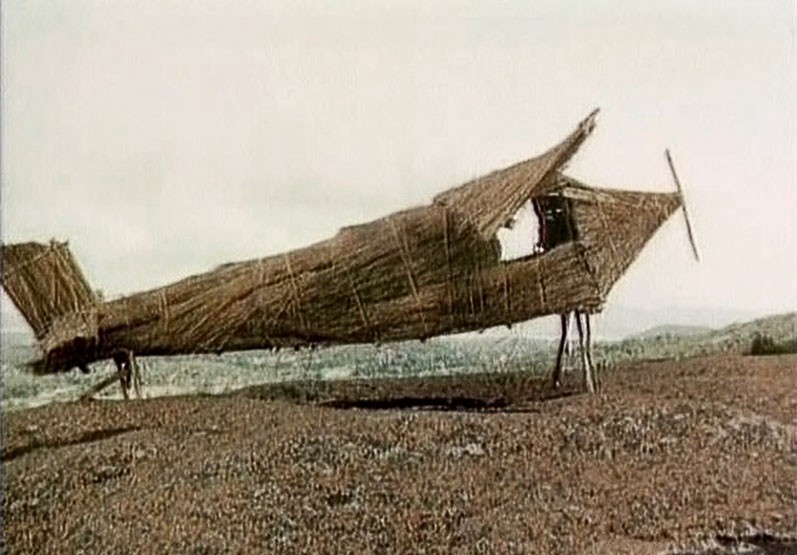
\includegraphics[scale=0.5]{cargo.jpeg}
\end{center}

\ifdefined\MyPrintFlag %%%% this is for printing a blank page
  \newpage
  \thispagestyle{empty}
  \ \\
\fi


\newpage
\tableofcontents


\newpage
\noindent
% of functional analysis and topology. It is needed because writing it by hand leads to severe amount of corrections, while implementing it with an interactive proof assistant is tedious and platform-dependent.\\
%\noindent
% elements are small letters, sets are uppercase latin letters, sets of sets are mathcal latin letters
% the code should be comprehensive: use meaning ozf symbols
Motivation: there are lots of proof assistants which allow to prove mathematical theorems, but their use for the purposes of an average mathematician is deeply disappointing due to various reasons.\\

I am creating a proof assistant and this document is a very early prologue to what the computer-generated article will look like.\\

The other point of creating such document is to provide programmed classical logical foundations for developing a set-theoretic proofs, and vice-versa to provide a set-theoretic foundations to prove theorems about logic.



\noindent
\subsection{Goals}
Despite theory being presented is sometimes unusually presented, my intention was to keep it as standard as possible. Any "extravagant" part has reason behind it: for example, it is absurd to speak about truthness of the statements $f(x)=5$, when $x\notin\dom(f)$.
We may want to say that it is false, but then it creates the assymetry: $f(x)\neq 5$ means that some of two cases is true: 1) $x\notin\dom(f)$ or 2) ($(x\notin\dom(f))$ and f(x) is actually equal to something else).
But when we have 3-valued logic, then we get rid of such compromises.
In it $(f(x)\neq 5)$ means that both sides are defined and they are not equal.\\

%The statement $f(x)\neq 5$ should not raise two different cases: whe



%Interesting targets:
\begin{itemize}
\item The aim of this document is to provide standard classical mathematical foundations as well as some amount of perfect proofs.
\item The proof assistant based on this very classical theory is being implemented. \url{https://github.com/georgydunaev/set_theory_prover}
\item After completion of development of the program, not only tactics, but also machine learning algorithms may be applied in a search of the proofs.

%\item sequential criterion
%\item completion of a metric space
\end{itemize}
%...
\newpage






%\section{Theorems within class theory}
%\section{Useful constructions in class theory}








%\section{References}
%\pagebreak
%\section{Acknowledgement}
%I am very grateful to these people for the knowledge they gave me.\\
%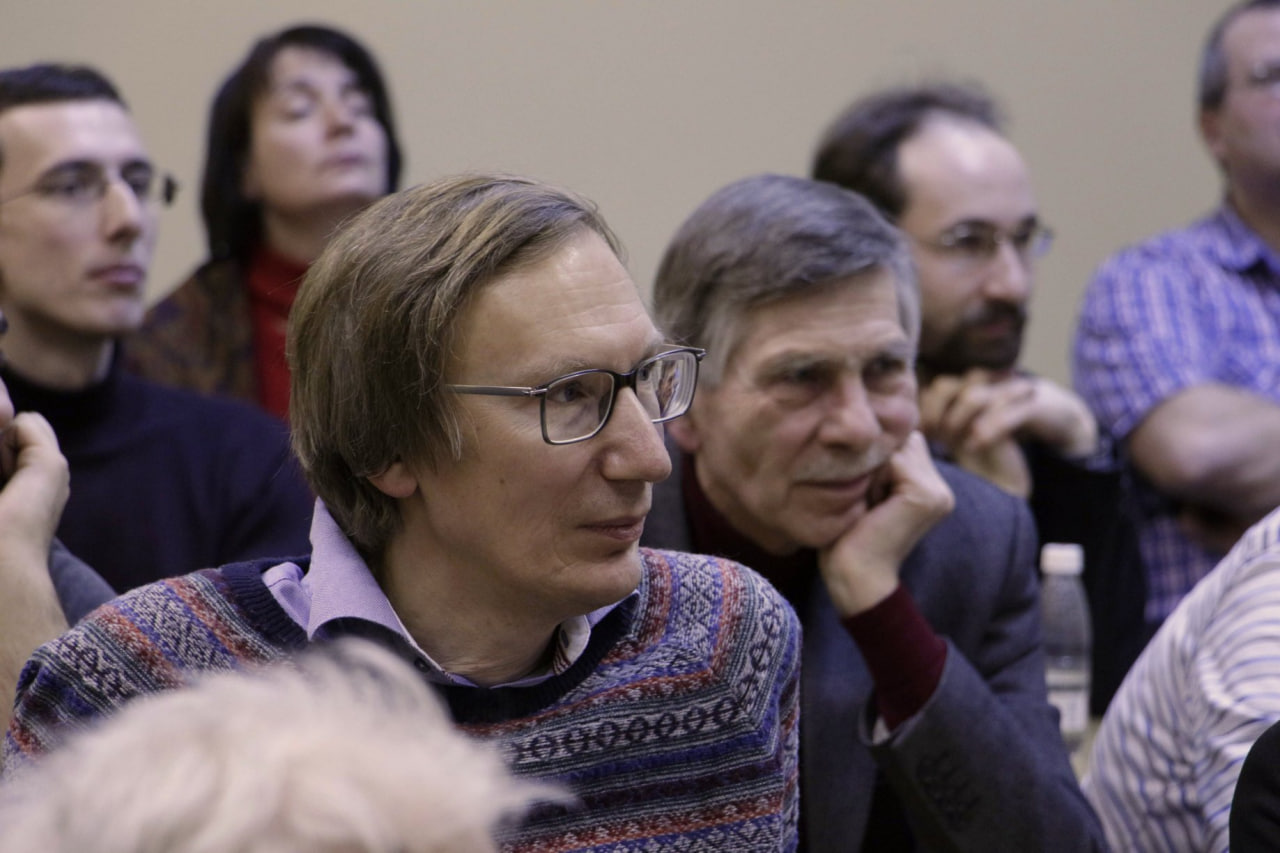
\includegraphics[scale=0.3]{Thanks.jpg}

%\begin{definition}
%Context: A algebra.\\
%\[
%\exists u\in A: \forall a\in A: (a-au)\in I \land (a-ua)\in I
%\]
%\end{definition}

%%% MODULES:

%
\ifdefined\MyHeaderIncluded

\else
  \newcommand{\foobar}{FooBar}
  \def\MyHeaderIncluded{true}
% if is till the end of the file

\documentclass[10pt,a4paper]{article}
\usepackage[utf8]{inputenc}
%\usepackage[german]{babel}
%\usepackage[cyrillic]{babel}
\usepackage[T1]{fontenc}
%\usepackage[T2A]{fontenc}
%\usepackage[english, russian]{babel}
\usepackage{amsmath}
\usepackage{amsfonts}
\usepackage{amssymb}
\usepackage{amsthm}
\usepackage{mathtools} %coloneqq

\usepackage{bussproofs} %

%\renewcommand{\thesubsection}{\arabic{subsection}}
%\newtheorem{thm}{Theorem}[section]
%\renewcommand{\thethm}{\arabic{subsection}.\arabic{thm}}

\usepackage{thmtools}
\usepackage{hyperref}
\hypersetup{
    colorlinks=true,
    linkcolor=blue,
    filecolor=magenta,      
    urlcolor=cyan,
    pdftitle={Overleaf Example},
    %pdfpagemode=FullScreen,
    }
%\usepackage{stix-type1}%\turnediota
\theoremstyle{definition}

\newtheorem{constructor}{Constructor}[section]
\newtheorem{iaxiom}{Axiom}
\newtheorem{axiom}{Axiom}
\newtheorem*{axiom*}{Axiom}
\newtheorem{definition}{Definition}[section]
\newtheorem*{definition*}{Definition}
\newtheorem{remark}{Remark}[section]
\newtheorem*{remark*}{Remark}
\newtheorem{recall}{Recall}[section]
\newtheorem*{recall*}{Recall}

\newtheorem{lemma}{Lemma}[section]
\newtheorem{theorem}{Theorem}[section]
\newtheorem*{theorem*}{Theorem}
\newtheorem{note}{Note}[section]
\usepackage{etoolbox}

%\newcommand*{\@Dashv}[2]{%
%  \reflectbox{$\m@th#1#2$}%
%}
\newcommand*{\separation}[3]{% 1)binder, 2)set, 3)condition
  \{#1\in #2: #3\}
}

% https://www.freecodecamp.org/news/simple-regex-tricks-for-beginners-3acb3fa257cb/
%  \\mathcal\{T\} |---> \topology
%  \\mathcal\{([^\}]*)\}   |--->  $1
\newcommand{\AND}{\ \ \&\ \ }
\newcommand{\any}{\mathrm{\ any}}
\newcommand{\borel}{\mathcal{B}}
\newcommand{\can}{\mathrm{can}}
\newcommand{\canonize}{\mathrm{canonize}}
\newcommand{\closure}{\mbox{cl}}
\newcommand{\complex}{\mathbb{C}}
\newcommand{\converges}{\longrightarrow}
\newcommand{\countable}{\mbox{\ countable}}
\newcommand{\ldefined}{\mbox{\ defined}}
\newcommand{\dom}{\mbox{dom}}
\newcommand{\Dom}{\mbox{Dom}}
\newcommand{\Done}{\noindent \textbf{Done.}\\}
\newcommand{\lexists}{\mbox{\ exists}}
\newcommand{\lforall}{\mbox{\ forall}}
\newcommand{\lunique}{\mbox{\ unique}}
\newcommand{\family}{\mathrm{\ family}}
\newcommand{\Fm}{\mathrm{Fm}}
\newcommand{\FuncSymb}{\mathrm{FuncSymb}}
\newcommand{\function}{\mathrm{\ function}}
\newcommand{\functional}{\mbox{\ functional}}
\newcommand{\IFF}{\ \Longleftrightarrow\ }
\renewcommand{\iff}{\ \longleftrightarrow\ }
\newcommand{\IMPLIES}{\ \Longrightarrow\ }
\renewcommand{\implies}{\ \longrightarrow\ }
\newcommand{\Inf}{\mathrm{Inf}}
\newcommand{\injective}{\mbox{\ injective}}
\newcommand{\injection}{\mbox{\ injection}}
\newcommand{\interior}{\mbox{int}}
\newcommand{\intersection}{\bigcap}
\newcommand{\isempty}{\mathrm{\ empty}}
\newcommand{\LB}{\mathrm{LB}}
\newcommand{\nghbset}{\mathcal{N}}
\newcommand{\nonempty}{\mathrm{\ nonempty}}
\newcommand{\Ord}{\mathrm{Ord}}
\newcommand{\power}{\mathcal{P}}
\newcommand{\pr}{\mathrm{pr}}
\newcommand{\fst}{\mathrm{fst}}
\newcommand{\snd}{\mathrm{snd}}
\newcommand{\PredSymb}{\mathrm{PredSymb}}
\newcommand{\Proof}{\noindent \textbf{Proof.}\\}
\newcommand{\ran}{\mathrm{ran}}
\newcommand{\Ran}{\mathrm{Ran}}
\newcommand{\real}{\mathbb{R}}
\newcommand{\relation}{\mathrm{\ relation}}
\newcommand{\set}{\mathrm{\ set}}
\newcommand{\singleton}{\mathrm{\ singleton}}
\newcommand{\semantics}{\mathrm{semantics}}
\newcommand{\semialgebra}{\mathcal{S}}
\newcommand{\Sup}{\mathrm{Sup}}
\newcommand{\surjective}{\mbox{\ surjective\ on\ }}
\newcommand{\Term}{\mathrm{Term}}
\newcommand{\Type}{\mathrm{Type}}
\newcommand{\topology}{\mathcal{T}}
\newcommand{\total}{\mbox{\ total\ on\ }}
\newcommand{\transitive}{\mathrm{\ transitive}}
\newcommand{\union}{\bigcup}
\newcommand{\lTrue}{\mathrm{True}}
\newcommand{\lFalse}{\mathrm{False}}
\newcommand{\lUncertain}{\mathrm{Uncertain}}
\newcommand{\lif}{\mathrm{if}}
\newcommand{\lthen}{\mathrm{then}}
\newcommand{\lelse}{\mathrm{else}}
\newcommand{\lexception}{\mathrm{exception}}
\newcommand{\lundef}{\mathrm{undef}}
\newcommand{\univocal}{\mathrm{\ univocal}}
\newcommand{\univocalat}{\mathrm{\ univocal\ at\ }}
\newcommand{\UB}{\mathrm{UB}}
\newcommand{\Un}{\mathcal{U}}
\newcommand{\Var}{\mathrm{Var}}

\newcommand{\notvarphi}{\phi}
\renewcommand{\phi}{\varphi}

\newcommand{\comment}[1]{\quad\mbox{(#1)}}
% local commands
%\preto\section{\undef\blipo} %etoolbox
\preto\subsection{\undef\blipo} %etoolbox
% https://tex.stackexchange.com/questions/105684/limit-macro-newcommand-scope-to-section
\usepackage{graphicx}
\usepackage{authblk}

\setlength\parindent{0pt} % whole doc of \noindent
\usepackage{soul}
%\usepackage{mathgl}

\fi % guard

\title{Supremum \& Infimum}
\author[1]{Georgy Dunaev}
\begin{document}
\maketitle
%Some order theory.
\section{Definitions}
\subsection{Upward/downward closed set}
\begin{definition}(Upward closed set)
\[
\uparrow_{(P,\leqslant)}x:=\{y\in P|x\leqslant y\}
\]
\end{definition}
\begin{definition}(Downward closed set)
\[
\downarrow_{(P,\leqslant)}x:=\{y\in P|y\leqslant x\}
\]
\end{definition}

\subsection{Ordered sets of majorants/minorants}
\begin{definition}(Ordered set of majorants)
\[
\mbox{Ma}_{(P,\leqslant)}S:=\left(\intersection \uparrow_{(P,\leqslant)}[S],\leqslant\right)
\]
\end{definition}
\begin{definition}(Ordered set of minorants)
\[
\mbox{Mi}_{(P,\leqslant)}S:=\left(\intersection \downarrow_{(P,\leqslant)}[S],\leqslant\right)
\]
\end{definition}
\subsection{Ordered sets of greatest/least elemenents}
\begin{definition}(Ordered set of greatest elements)
\[
\mbox{Greatest}_{(P,\leqslant)}:=\mbox{Ma}_{(P,\leqslant)}P
\]
\end{definition}
\begin{definition}(Ordered set of least elements)
\[
\mbox{Least}_{(P,\leqslant)}:=\mbox{Mi}_{(P,\leqslant)}P
\]
\end{definition}
\subsection{Ordered sets of supremums/infimums}
\begin{definition}(Ordered set of supremums)
\[
\mbox{Sup}_{(P,\leqslant)}S:=\mbox{Least}_{\mbox{Ma}_{(P,\leqslant)}S}
\]
\end{definition}
\begin{definition}(Ordered set of infimums)
\[
\mbox{Inf}_{(P,\leqslant)}S:=\mbox{Greatest}_{\mbox{Mi}_{(P,\leqslant)}S}
\]
\end{definition}




%\begin{theorem}
%\[
%(A\set)
%\implies
%\left(\union A\set\right)
%\]
%\end{theorem}
%\Proof
%(the proof needs theorems about ordinals done first)\\
%...\\
%\Done


\end{document}
\def\topic{Chapter: Logic}%Foundations of mathematics
\ifdefined\MyHeaderIncluded
\else
\def\qwertyflag{true}

\ifdefined\MyHeaderIncluded

\else
  \newcommand{\foobar}{FooBar}
  \def\MyHeaderIncluded{true}
% if is till the end of the file

\documentclass[10pt,a4paper]{article}
\usepackage[utf8]{inputenc}
%\usepackage[german]{babel}
%\usepackage[cyrillic]{babel}
\usepackage[T1]{fontenc}
%\usepackage[T2A]{fontenc}
%\usepackage[english, russian]{babel}
\usepackage{amsmath}
\usepackage{amsfonts}
\usepackage{amssymb}
\usepackage{amsthm}
\usepackage{mathtools} %coloneqq

\usepackage{bussproofs} %

%\renewcommand{\thesubsection}{\arabic{subsection}}
%\newtheorem{thm}{Theorem}[section]
%\renewcommand{\thethm}{\arabic{subsection}.\arabic{thm}}

\usepackage{thmtools}
\usepackage{hyperref}
\hypersetup{
    colorlinks=true,
    linkcolor=blue,
    filecolor=magenta,      
    urlcolor=cyan,
    pdftitle={Overleaf Example},
    %pdfpagemode=FullScreen,
    }
%\usepackage{stix-type1}%\turnediota
\theoremstyle{definition}

\newtheorem{constructor}{Constructor}[section]
\newtheorem{iaxiom}{Axiom}
\newtheorem{axiom}{Axiom}
\newtheorem*{axiom*}{Axiom}
\newtheorem{definition}{Definition}[section]
\newtheorem*{definition*}{Definition}
\newtheorem{remark}{Remark}[section]
\newtheorem*{remark*}{Remark}
\newtheorem{recall}{Recall}[section]
\newtheorem*{recall*}{Recall}

\newtheorem{lemma}{Lemma}[section]
\newtheorem{theorem}{Theorem}[section]
\newtheorem*{theorem*}{Theorem}
\newtheorem{note}{Note}[section]
\usepackage{etoolbox}

%\newcommand*{\@Dashv}[2]{%
%  \reflectbox{$\m@th#1#2$}%
%}
\newcommand*{\separation}[3]{% 1)binder, 2)set, 3)condition
  \{#1\in #2: #3\}
}

% https://www.freecodecamp.org/news/simple-regex-tricks-for-beginners-3acb3fa257cb/
%  \\mathcal\{T\} |---> \topology
%  \\mathcal\{([^\}]*)\}   |--->  $1
\newcommand{\AND}{\ \ \&\ \ }
\newcommand{\any}{\mathrm{\ any}}
\newcommand{\borel}{\mathcal{B}}
\newcommand{\can}{\mathrm{can}}
\newcommand{\canonize}{\mathrm{canonize}}
\newcommand{\closure}{\mbox{cl}}
\newcommand{\complex}{\mathbb{C}}
\newcommand{\converges}{\longrightarrow}
\newcommand{\countable}{\mbox{\ countable}}
\newcommand{\ldefined}{\mbox{\ defined}}
\newcommand{\dom}{\mbox{dom}}
\newcommand{\Dom}{\mbox{Dom}}
\newcommand{\Done}{\noindent \textbf{Done.}\\}
\newcommand{\lexists}{\mbox{\ exists}}
\newcommand{\lforall}{\mbox{\ forall}}
\newcommand{\lunique}{\mbox{\ unique}}
\newcommand{\family}{\mathrm{\ family}}
\newcommand{\Fm}{\mathrm{Fm}}
\newcommand{\FuncSymb}{\mathrm{FuncSymb}}
\newcommand{\function}{\mathrm{\ function}}
\newcommand{\functional}{\mbox{\ functional}}
\newcommand{\IFF}{\ \Longleftrightarrow\ }
\renewcommand{\iff}{\ \longleftrightarrow\ }
\newcommand{\IMPLIES}{\ \Longrightarrow\ }
\renewcommand{\implies}{\ \longrightarrow\ }
\newcommand{\Inf}{\mathrm{Inf}}
\newcommand{\injective}{\mbox{\ injective}}
\newcommand{\injection}{\mbox{\ injection}}
\newcommand{\interior}{\mbox{int}}
\newcommand{\intersection}{\bigcap}
\newcommand{\isempty}{\mathrm{\ empty}}
\newcommand{\LB}{\mathrm{LB}}
\newcommand{\nghbset}{\mathcal{N}}
\newcommand{\nonempty}{\mathrm{\ nonempty}}
\newcommand{\Ord}{\mathrm{Ord}}
\newcommand{\power}{\mathcal{P}}
\newcommand{\pr}{\mathrm{pr}}
\newcommand{\fst}{\mathrm{fst}}
\newcommand{\snd}{\mathrm{snd}}
\newcommand{\PredSymb}{\mathrm{PredSymb}}
\newcommand{\Proof}{\noindent \textbf{Proof.}\\}
\newcommand{\ran}{\mathrm{ran}}
\newcommand{\Ran}{\mathrm{Ran}}
\newcommand{\real}{\mathbb{R}}
\newcommand{\relation}{\mathrm{\ relation}}
\newcommand{\set}{\mathrm{\ set}}
\newcommand{\singleton}{\mathrm{\ singleton}}
\newcommand{\semantics}{\mathrm{semantics}}
\newcommand{\semialgebra}{\mathcal{S}}
\newcommand{\Sup}{\mathrm{Sup}}
\newcommand{\surjective}{\mbox{\ surjective\ on\ }}
\newcommand{\Term}{\mathrm{Term}}
\newcommand{\Type}{\mathrm{Type}}
\newcommand{\topology}{\mathcal{T}}
\newcommand{\total}{\mbox{\ total\ on\ }}
\newcommand{\transitive}{\mathrm{\ transitive}}
\newcommand{\union}{\bigcup}
\newcommand{\lTrue}{\mathrm{True}}
\newcommand{\lFalse}{\mathrm{False}}
\newcommand{\lUncertain}{\mathrm{Uncertain}}
\newcommand{\lif}{\mathrm{if}}
\newcommand{\lthen}{\mathrm{then}}
\newcommand{\lelse}{\mathrm{else}}
\newcommand{\lexception}{\mathrm{exception}}
\newcommand{\lundef}{\mathrm{undef}}
\newcommand{\univocal}{\mathrm{\ univocal}}
\newcommand{\univocalat}{\mathrm{\ univocal\ at\ }}
\newcommand{\UB}{\mathrm{UB}}
\newcommand{\Un}{\mathcal{U}}
\newcommand{\Var}{\mathrm{Var}}

\newcommand{\notvarphi}{\phi}
\renewcommand{\phi}{\varphi}

\newcommand{\comment}[1]{\quad\mbox{(#1)}}
% local commands
%\preto\section{\undef\blipo} %etoolbox
\preto\subsection{\undef\blipo} %etoolbox
% https://tex.stackexchange.com/questions/105684/limit-macro-newcommand-scope-to-section
\usepackage{graphicx}
\usepackage{authblk}

\setlength\parindent{0pt} % whole doc of \noindent
\usepackage{soul}
%\usepackage{mathgl}

\fi % guard
\ifdefined\topic
\else
\def\topic{No Titel}
\fi
\title{\topic}
\author[1]{Georgy Dunaev}
\begin{document}
\maketitle
\fi
%\section{Logical framework}%First-order l

%\begin{definition}(conglomerate of all classes)
%\
%\end{definition}
%\sub
\newgeometry{left=1cm, right=3cm, top=3cm, bottom=3cm} 
\section{Example of the proof assistant's output}

This chapter develops several related projects: a notation for manipulating
syntax in a proof assistant, a classical predicate calculus, and a framework
for comparing effective proof with an ideal, non-effective foundational theory.
Each project has its own assumptions. In particular, a computation on syntax,
a derivation in a theory, and truth in an intended interpretation are different
notions; the notation introduced below is intended to make their interaction
explicit. The historical semantic experiments retained in the source use
additional conventions of their own.

The screenshot below illustrates tests of a kernel that stores proof objects.
Storing the entire derivation is an implementation choice; it is distinct from
checking that each inference is licensed by the kernel.

The motivating question is how much metatheory can be represented
\textit{syntactically} inside the theory. Encoding a metatheoretic statement is
only the first step: a rule that reflects that statement back into the theory
needs its own justification. A related approach represents a theory
\textit{semantically}, through an inner model. These approaches serve different
purposes. The later sections explore a framework for discussing incompleteness
while keeping these levels visible.

% тип полностью или неполнстью определён
% тип написан как объект (и это возможно)
% тип написан как терм, но можно было как объект
% тип написан как объект (и это было невозможно) -- неполная имплементация/ошибка
% тип написан как терм, но можно было как объект

\begin{informaldefinition}[syntactic and semantic types]
A guest type $A$ in a [conglomerate--level] type theory of this book is called \textit{syntactic} if its intended meaning -- as a ``collection'' of ``elements'' of some size -- is ``bijectively representable'' in the host language. That is, there exists a host type $T$ such that:
\begin{enumerate}
\item There is a bijection between the ``intended meanings'' of the terms of the guest type $A$ and the terms of the host type $T$.
%\item    Every element $a$ of the collection denoted by $A$ corresponds to a unique term $t$ of type $T$, and
%\item    Every term $t$ of type $T$ corresponds to a unique element $a$ of the collection denoted by $A$.
\item    In particular, the interpretation of $A$ as a ``collection'' is ``effectively'' given by its image in $T$: the representation must specify how a term of type $T$ is read as an element of $A$. This is an informal representability requirement; a claim of computability would additionally require an explicit encoding and decoding procedure.
\end{enumerate}
\end{informaldefinition}


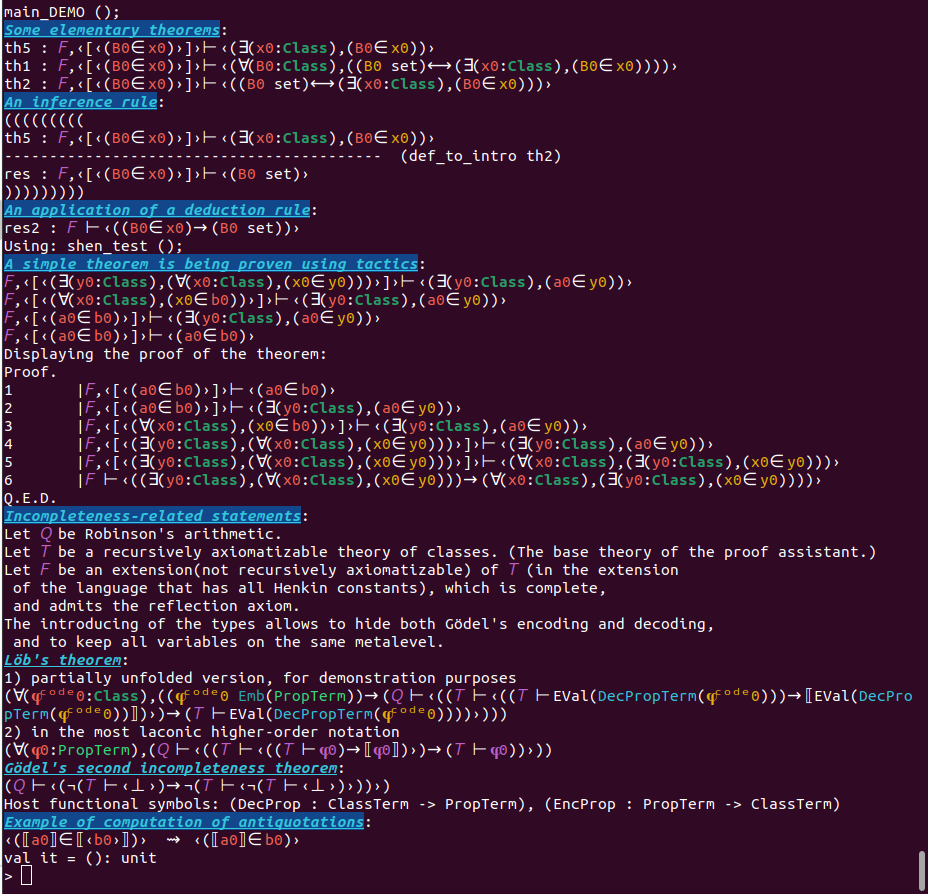
\includegraphics[scale=0.5]{pictures/DEMO.png}

%\restoregeometry
\pagebreak
%\newgeometry{left=1cm, right=3cm, top=3cm, bottom=3cm} 

\section{Type theory of the proof assistant}
The book also documents a proof assistant. Its architecture is inspired by the
LCF approach: a small kernel controls the construction of certified theorems,
while higher-level code organises proofs. The type notation below describes
syntactic objects manipulated by that implementation. It must be distinguished
from the classes and types discussed inside an object theory.

%\iffalse
\IfFileExists{../set_theory_prover/program/CONTENT.ML}{%
\begin{nolinenumbers}
\lstinputlisting[basicstyle=\ttfamily\footnotesize]{../set_theory_prover/program/CONTENT.ML}
\end{nolinenumbers}
}{%
\begin{note}[companion implementation]
The full datatype listing belongs to the companion proof-assistant project
and is not included in this checkout. The definitions and notation below
provide the reading conventions needed for this chapter.
\end{note}
}
%\fi

\restoregeometry
\subsection{Primitive definitions and notation}
\begin{definition}[variable]
A \textit{variable} is an ordered pair consisting of a string, called its \textit{name}, and a natural number, called its \textit{level}. The two components record the identifier and its metalevel in the syntactic representation.
\end{definition}
The companion code gives the corresponding datatype constructors. The mathematical notation below suppresses some of those constructors, so the translation conventions are stated explicitly. %(Especially during the development.)\\
%For any variables $x$,$\phi$,\dots , define
%\subsection{Meaning of dots and bold symbols}%Second bold notation
The following examples connect the typed notation of the implementation with ordinary mathematical notation.
%this subsection. 
%the following subsection.

The comparison begins with representability in arithmetic, then records the proposed encoding in the notation of this book:
\begin{definition*}[representability in the traditional notation]
Let $\mathbb{N}$ be the set of natural numbers. A %first--order
theory $T$ in the language of arithmetic containing $\mathsf{Q}$ ``represents'' the $k$--ary recursive function $f: \mathbb{N}^k\rightarrow\mathbb{N}$ if there is a formula $\varphi_f(x_1, \dots, x_k, y)$ in the language of $T$ s.t. for all $m_1, \dots, m_k \in \mathbb{N}$, if $f(m_1, \dots, m_k) =  n$ then \[
T \vdash \forall y (\varphi_f (\overline{m_1}, \dots, \overline{m_k}, y) \iff y = \overline{n} ).
\]
(\url{https://en.wikipedia.org/wiki/Diagonal_lemma#Representation_Theorem})
\end{definition*}
\begin{example*}[representability in the proposed higher-order notation]
The displays below explore how to encode the preceding definition. Their
intended common meaning is the preceding representability condition. A fully
typed translation still requires the domains of quotation, antiquotation,
and substitution to be fixed; the displays are not separate representation
theorems.
Let $\mathbb{N}$ be the set of natural numbers. 
A% first--order
 theory $T$ in the language of arithmetic containing $\mathsf{Q}$ ``represents'' the $k$--ary recursive function $f: \mathbb{N}^k\rightarrow\mathbb{N}$ if there is a formula $\varphi_f(x_1, \dots, x_k, y)$ in the language of $T$ s.t. 
for all $m_1, \dots, m_k \in \mathbb{N}$, if $f(m_1, \dots, m_k) =  n$ then 
\iffalse
\[
T \vdash \Quote\Fm(\forall y (\Antiquote\Fm(\varphi_f)[\Antiquote\Class(m_1)/x_1, \dots, \Antiquote\Class(m_k)/x_k, y/y] \leftrightarrow (y = \Antiquote(n)) )).
\]
\fi
\[
T \vdash \Quote\Fm(\forall y (\Antiquote\Fm(\varphi_f[m_1/x_1, \dots, m_k/x_k, \Quote(y)/y]) \leftrightarrow (y = \Antiquote(n)) )).
\]
A proposed alternative display, whose typing remains to be checked, is
\[
T \vdash (\forall \Quote(y), ((\varphi_f[m_1/x_1, \dots, m_k/x_k, \Quote\Class(y)/y]) \iff (\Quote\Class(y) = n) )).
\]
Another proposed display is
\[
T \vdash (\forall y, ((\varphi_f[m_1/x_1, \dots, m_k/x_k, \Quote\Class(y)/y]) \iff (\Quote\Class(y) = n) )).
\]
For comparison, the shorter assertion notation is:
\[
T \vdash \llcorner \pmb{\varphi} \lrcorner
\]

The corresponding expanded display is
\[
T \vdash \llcorner
\pmb{ \forall } \pmb{y} \pmb{(}\pmb{\varphi}_{\pmb{f}} \pmb{(}\boldmeta{m_1}\pmb{,} \pmb{\dots}\pmb{,} \boldmeta{m_k}\pmb{,} \pmb{y}\pmb{)} \pmb{\leftrightarrow} \pmb{y} = \boldmeta{n} \pmb{)}\lrcorner,
\]
where
\[
\ulcorner\cdot\urcorner \equivdef (\text{AntiquoteClass} \circ \EncFm),
\]
\[
\ulcorner\cdot\urcorner : \Fm \to \Class
\]
\[
\llcorner\cdot\lrcorner \equivdef (\DecFm \circ \text{QuoteClass}).
\]%(\DecFm \circ \text{QuoteClass})
%\DecFm
\[
\llcorner\cdot\lrcorner : \ClassTerm \to \Fm
\]
For any formula $\phi$,
\[
\llcorner\ulcorner\phi\urcorner\lrcorner
\equiv
\phi.
\]
\end{example*}
\begin{example}[extension rule]
The following proposed \textit{extension rule} records a further design question.
The question marks mark domains that have not yet been specified:
\[
\forall (\varphi:\Fm),\ %
(\Fau \vdash \forall (n:?),\ \llcorner \pmb{\varphi}(\boldmeta{n}) \lrcorner)
\IMPLIES
(\Fau \vdash \forall (n:?),\ \varphi(n) ),
\]
\[
\forall (\varphi:\Fm),\ %
(\forall (n:\ClassTerm),\ \Fau \vdash \llcorner \pmb{\varphi}(\boldmeta{n}) \lrcorner)
\IMPLIES
(\Fau \vdash \forall (n:\Class),\ \varphi(n) ),
\]

Here the operation denoted by $\varphi(n)$, the domains of the two quantifiers,
and the hypotheses licensing passage from all instances to a universal
statement remain to be defined. This example is a proposed rule, not an
admissibility result.
\end{example}

\iffalse % VERY GOOD, BUT DISTRACTING
\subsection{First bold notation}
\subsubsection{Notation for variables}
\begin{notation}[bold variables for terms]
For any lower-case Latin letter(e.g. `x'), define a bold lower-case Latin letter to denote

%val xb1 : Class = (CShiftClass (Quote(CV (namelvl (`x',zero)))))
\begin{lstlisting}
val xb1 : Class = (QuoteClass (CV (namelvl (`x',zero))))
val yb1 : Class = (QuoteClass (CV (namelvl (`y',zero))))
...
\end{lstlisting}
Equivalently, suppressing datatype constructors in the mathematical notation,
\[
\pmb{x} \equivdef \Quote\Var( x_{(0)} ),
\]
\[
\pmb{y} \equivdef \Quote\Var( y_{(0)} ),
\]
\[
\dots
\]
\end{notation}%and so on.

\begin{notation}[bold variables for formulas]
For any lower--case Greek letter(`{$\phi$}',`{$\psi$}', `{$\chi$}', \dots), define a bold lower-case Greek letter to denote
\begin{lstlisting}
val phib1 : Class = (QuoteFm (FmVar vphi))
val psib1 : Class = (QuoteFm (FmVar vpsi))
...
\end{lstlisting}
Equivalently, suppressing datatype constructors in the mathematical notation,
\[
\pmb{\phi} \equivdef \Quote\Fm( \phi_{(0)} ),
\]
\[
\pmb{\psi} \equivdef \Quote\Fm( \psi_{(0)} ),
\]
\[
\dots
\]
\end{notation}

\subsubsection{Notation for functional and predicate symbols}
All bald functional and predicate symbols written boldly simply mean the same constructors as their thin counterparts.
\pagebreak

\fi %VERY GOOD BUT DISTRACTING (First bold notation)

\subsection{Meaning of dots and bold symbols}%Second bold notation
%The second bold notation may be introduced in a situation when it is useful to show that 
The intended translation represents higher-order syntax by first-order codes,
using encoding/decoding together with quotation/antiquotation. The identities
below specify the intended behaviour on well-formed inputs; they do not by
themselves establish a translation theorem for the entire framework.

This subsection uses $\Fm$ as the running example. Analogous conventions are intended for the other syntactic types: $\Ctx$, $\Class$, $\Theory$, etc.%labeled by : for
\begin{definition}[functions Bold and Dot]
Let $\circ$ be an infix operator of composition of functional symbols here. Then
\[
\text{BoldFm} \equivdef \EncFm
\]%(\EncFm \circ \text{QuoteFm})
\[
\text{BoldFm} : \Fm \to \ClassTerm 
\]
and
\[
\text{Dot} \equivdef (\text{AntiquoteClass}).%\circ \DecFm
\]
\[
\text{Dot} : \ClassTerm \to \ClassTerm 
\]

\end{definition}

\begin{notation}[bold and/or dotted variables for formulas]
For a formula variable $\phi$, its encoding is denoted as a bold $\pmb{\phi}$:
\[
\pmb{\phi} \equivnot \text{BoldFm}(\phi).
\]
For any class variable $t$, its antiquotation is denoted with a dot:
\[
\meta{t} \equivnot \text{Dot}(t).
\]
\end{notation}

\begin{note}[non--commutativity of notation]
%Contrary to the first notation,
Boldface and a dot denote operations applied in a specified order:
%\iffalse good
\iffalse
\[
\meta{\pmb{\phi}} \equivdef \text{BoldFm}(\text{DotFm}(\phi)).
\]
\fi
\[
\meta{\pmb{\phi}} \equivnot \text{Dot}(\text{BoldFm}(\phi)).
\]
%where
\iffalse
\[
\text{BoldFm} \equivdef (\EncFm \circ \text{Quote})
\]
and
\[
\text{DotFm} \equivdef (\text{Antiquote} \circ \DecFm).
\]
\fi
After the corresponding decoding step, the round trip is intended to recover the original formula:
\iffalse
\[
\meta{\pmb{\phi}} 
\equiv 
((\EncFm \circ \Quote) \circ (\Antiquote \circ \DecFm))(\phi)
\equiv
\phi
\]%\EncFm(\Antiquote(\phi))

\[
\meta{\pmb{\phi}} 
\equiv 
((\DecFm \circ \Quote) \circ (\Antiquote \circ \EncFm))(\phi)
\equiv
\phi
\]%\EncFm(\Antiquote(\phi))
\fi
\iffalse %last before three--agreement
\[
\meta{\pmb{\phi}} 
\equiv 
(
(\DecFm \circ \text{QuoteClass})
\circ
(\text{AntiquoteClass} \circ \EncFm)
)(\phi)
\equiv
\phi
\]%\EncFm(\Antiquote(\phi))
No!%(\DecFm \circ \text{QuoteClass})
\fi
\[
\llcorner
\meta{\pmb{\phi}} 
\lrcorner
\equiv 
(
(\DecFm \circ \Quote\Class)
\circ
(\text{AntiquoteClass})%\circ \DecFm
\circ
(\EncFm)
)(\phi)
\equiv
\phi
\]%\EncFm(\Antiquote(\phi))
%%%(\text{AntiquoteClass} \circ \DecFm)

So the following computational equality is an identity:
\[
\boxed{
\llcorner
\meta{\pmb{\phi}} 
\lrcorner
\equiv 
\phi
}
\]
%\[
%\pmb{\dot{\phi}} \equivdef \text{Bold}(\text{Meta}(\phi))
%\] % too ugly
\end{note}

\subsubsection{Notation for variables}
\begin{notation}[bold variables for terms]
For a lower-case Latin letter, such as ``x'', boldface denotes the encoded variable:
\iftrue
\begin{lstlisting}
val xb : Class = (EncClass (CV (namelvl ("x", Nat.zero))))
val yb : Class = (EncClass (CV (namelvl ("y", Nat.zero))))
...
\end{lstlisting}
\fi
\begin{lstlisting}
\end{lstlisting}
Equivalently, suppressing datatype constructors in the mathematical notation,
\[
\pmb{x} \equivdef \EncClass(x_{(0)} ),
\]
\[
\pmb{y} \equivdef \EncClass( y_{(0)} ),
\]
\[
\dots
\]
\end{notation}%and so on.

\begin{notation}[bold variables for formulas]
For any lower--case Greek letter(`{$\phi$}',`{$\psi$}', `{$\chi$}', \dots), define a bold lower-case Greek letter to denote
\begin{lstlisting}
val phib : Class = (EncFm (FmVar vphi))
val psib : Class = (EncFm (FmVar vpsi))
...
\end{lstlisting}
Equivalently, suppressing datatype constructors in the mathematical notation,
\[
\pmb{\phi} \equivdef \EncFm(\phi_{(0)} ),
\]
\[
\pmb{\psi} \equivdef \EncFm(\psi_{(0)} ),
\]
\[
\dots
\]
\end{notation}

\subsubsection{Notation for functional and predicate symbols}
Bold function and predicate notation denotes constructors acting on codes.
Encoding is therefore described inductively, one syntactic constructor at a time:

\begin{definition}[computation of the encoding of statements]
For a theory term $\Wau$, a context term $\Gamma$, and a formula term $\phi$,
\[
\EncStmt(\Wau,\,\Gamma\vdash \phi)
\equiv
\pmb{(} \EncTheory(\Wau) \pmb{,}\, \EncCtx(\Gamma)\pmb{\pmb{\vdash}} \EncFm(\phi)\pmb{)}
\]
\end{definition}
The right-hand side applies a first-order function symbol to the codes of the
three arguments. Its value represents the code of the whole statement. Other
syntactic constructors are encoded in the same way.

\iffalse
\begin{definition}
A term is called a \textit{class--term}, when it's a term of the type which is, unfortunately confusingly, called $\Term$ in the source code.
\end{definition}
\fi


\subsection{Definitions of inference--related constants and their notation}
\iffalse
\subsection{OBSOLETE PART TO BE DELETED}

\begin{definition}[informal introduction]
Let $\Fm,\ClassTerm,\Ctx,\Theory,...$ be a finite amount of sets, consisting of formulas, terms, contexts, theories, etc, in a model of Standard ML language. There is a model, and the precise construction of it is outside of the scope of this book,let's just assume that there is one, and therefore there is one in a foundational theory $\Fau$, so there is a (computable) function from syntactic entities  to certain objects in a domain of discussion $C$, which is a conglomerate of all classes.\\

In a such model of Standard ML, there is a typing relation between semantics of terms and types.\\
Assume this relation is given.\\
Then let's restrict it, for simplicity, to only those aforementioned types $\Fm,\ClassTerm,\Ctx,\Theory,...$ and their ground values (without variables).\\
Then let's extend this typing relation to the extended one, in which all remaining types also have type $\Type$, such that 
$(\Fm:\Type)$, $(\Class:\Type)$, $(\Ctx:\Type)$, $\dots$
%, $(\Typ:\Typ)$ (note the last one).\\
This could lead to a contradiction (Girard's Paradox) in case if this typing system would be significantly richer: at least if it had types of functions, dependent types, etc, but it doesn't have any of that: it is as simple as possible.
\end{definition}
%, even finite.
\fi

%class constants, corresponding to codes of syntactic entities
\begin{definition}[sets of codes]
%Let $\circ$ be a composition of functional symbols here, then t
The following class constants represent the codes of formulas, class terms, contexts, and the other syntactic datatypes:
\[
\text{FmCode} 
\equivdef
\CFm
\text{, where }
\CFm
\equivdef
\Emb(\TFm)
\]
\[
\text{ClassCode} 
\equivdef
\CClass
\text{, where }
\CClass
\equivdef
\Emb(\TClass)
\]
\[
\dots
\]
\end{definition}
\iffalse
\begin{notation}[overloading]
Luckily, on paper, it is possible to completely avoid the necessity of coloring the constants or of writing prefixes, via simple overloading trick: 
\[
\text{FmCode}
\equivnot
\CFm
\]
\[
\text{ClassCode}
\equivnot
\CClass
\]
\[
\dots
\]
Unfortunately, the Standard~ML doesn't have the overloading feature, so prefixes are kept in the program.
\end{notation}
\fi


%(\text{Enc}\circ\text{VTyp})

%It is possible for
%\TClass is an element


\iffalse
\begin{notation}[abuse of notation]
It seems possible to identify $\ClassTerm$ and $\TClass$, but it will not be done to avoid confusion.
%The author is not sure, where 
%(but in fact, no)
%It can be
%Starting from the next chapter, it can be 
%It seems like
%\[
%\ClassTerm = \TClass = \text{CClass}
%\]
\end{notation}
\fi
\subsection{Typed quantification and its notation}
Typed quantification over syntactic objects is represented below by
quantification over their codes. A code variable must be fresh for the body,
and every displayed substitution is capture-avoiding. Quantification over
semantic classes is a separate issue: the set- and class-quantifier schemes
later in this subsection are proposed axioms, not consequences of the
coding convention alone.
\begin{definition}[quantifiers with a bound variable of type $\Fm$]
Let $\phi$ be a variable for formulas.\\
Let $\psi$ be a formula.\\
% such that $\phi_code$ is not free in $\phi$.
%Not enough.
Choose a fresh code variable $\phi_\code$. Assume also that the substitution
$\psi[(\DecFm(\phi_\code))/\phi]$ is computed successfully, i.e. without raising an exception or error.
Then
%Then the following formula 
\[
(\forall (\phi:\TFm),\ \psi)
\iffdef
\]
\[
\iffdef
(\forall (\phi_\code:\TClass),\ %
(\phi_\code\in \Emb(\TFm))
\implies
\psi[
\DecFm(\phi_\code)
/
\phi
]
)
\]
\end{definition}
% bad1: (\text{Enc}\circ\text{VTyp})
% bad2: (\text{ValToFm}\circ\text{Dec})
\begin{notation}[naming prefix of labels]
Standard~ML distinguishes type names from values. Here the datatype named
Type has value constructors with the prefix ``T'', such as ``TFm'',
``TClass'', and ``TCtx''. The prefix helps distinguish a syntactic type label
from the datatype of expressions that carry that label.\\
In mathematical displays we suppress the prefix when the context determines
its meaning. Thus, instead of the explicit label
\[
``(\forall(\phi:\TFm),\ \dots)",
\]
starting from the next chapter, it will be written
\[
``(\forall(\phi:\Fm),\ \dots)".
\]
\end{notation}
\iffalse
\begin{notation}[overloading naming prefix of constants]
Similarly, instead of more precise expression
\[
``(\forall(f\in\CFm),\ \dots)",
\]
it will be written
\[
``(\forall(f\in\FmCode),\ \dots)".
\]
Note, that the letter $f$ here is a vareiable for the code of the formula, not for the formula itself, as was above where the symbol ``:'' was used.
\end{notation}
\fi
Other changes between syntactic and semantic notation will be stated explicitly.% at all costs.


%Now the tricky part, te

\begin{axiom}[set terms quantification unfolds via itself]
The proposed set-quantifier scheme retains a set-typed code quantifier:
\[
(\forall (t:\TSet),\ \psi)
\iffaxm
\]
\[
\iffaxm
(\forall (t_\code:\TSet),\ %
(t_\code\in \Emb(\TSet))
\implies
\psi[
\DecSet(t_\code)
/
t
]
)
\]
Here $t_\code$ is fresh for $\psi$. The scheme is stated as an axiom because
the same quantifier appears on both sides; it is not a recursive definition.
Its semantic justification is an additional obligation of this proposed model.
\end{axiom}
\begin{notation}[overloading class bindings]
Again, as previously for formulas, a formula
\[
``(\forall(K:\TSet),\ \dots)"
\]
can be written as
\[
``(\forall(K:\Set),\ \dots)".
\]
\iffalse
and also the quantifiers bound by a variable codes of definable classes
\[
``(\forall(e\in\CClass),\ \dots)"
\]
can be likewise unambiguously written as
\[
``(\forall(e\in\ClassCode),\ \dots)".
\]
\fi
\end{notation}
%########################## Class

\begin{axiom}[class terms quantification unfolds via itself]
The analogous proposed class-quantifier scheme retains a class-typed code
quantifier. Its typing predicate requires the interpretation supplied by the
model of pi-types.
\[
(\forall (t:\TClass),\ \psi)
\iffaxm
\]
\[
\iffaxm
(\forall (t_\code:\TClass),\ %
(t_\code : \Emb(\TClass))
\implies
\psi[
\DecClass(t_\code)
/
t
]
)
\]
Here $t_\code$ is fresh for $\psi$. The scheme is stated as an axiom because
the same quantifier appears on both sides; it is not a recursive definition.
Its semantic justification is an additional obligation of this proposed model.
\end{axiom}
\begin{notation}[overloading class bindings]
Again, as previously for formulas, a formula
\[
``(\forall(K:\TClass),\ \dots)"
\]
can be written as
\[
``(\forall(K:\Class),\ \dots)".
\]
\end{notation}

% ###

\begin{notation}[the default type]
In class-theoretic formulas, an omitted type annotation means ``Class'':
\[
(\forall K,\ \psi)
\iffnot
(\forall (K:\Class),\ \psi)
\]
Thus an unqualified ``term'' in that context means a class term. In discussions
of implementation or syntax, the relevant datatype is stated separately.
\end{notation}
\iffalse% METALANG
\section{Metalanguage[section is not yet finished]}
Usually, when something is proven, questions arise: ``Where it was proven?'', ``What was a foundational theory?'', ``What was a metatheory of the statement?''. Unfortunately, once the answers are established for the theory, the same questions may be asked about metatheory, metametatheory, and so on.\\
To avoid this ``infinite descend'' with increasing complexity of the statement of each step, author proposes to use a certain theory $\mathcal{F}$ as it's own metatheory, so the questions about the metatheory can be discussed in the theory itself.\\%is possible to answer within a theory.\\
In fact, a prefix ``$\mathcal{F}\vdash$'' is virtually omnipresent near every formula of this book, but it is not written, since the act of actual writing of it leads to the increase of complexity and increase of a metalevel of the statement.\\
\begin{definition}[level of meta]
Metalevel of the statement is the maximal amount of nested ``$\mathcal{F}\vdash (\dots)$'' in the formula.
\end{definition}


%Metatheory:\\
During reading the string of symbols, it is important to distinguish entities which are semantic(e.g. a set $\emptyclass$ or a proposition $(\emptyclass \in \omega)$) from their symbols which are syntactic and belonging to metatheory (e.g. a term $\ulcorner\boldemptyclass\urcorner$, and a judgement $(\ulcorner\boldemptyclass\urcorner : \Class)$). The symbols $``\ulcorner\cdot\urcorner"$ are used to explicitly show that that the object inside is syntactic, i.e. is a word. 


%%%%% May be useful:
%%%%% Currently, they are often omitted, but the the rule of thumb is that in chapters devoted to logic, syntactic entities are written, and in chapters devoted to mathematics, semantic entities are written. Moreover, to avoid confusion, and due to computational properties of syntactic entities, it is natural to use a naive type theory for logic parts, so it makes it is easy to distinguish syntax from semantics.


A sufficiently expressive programming language of reader's choice, may be used for implementing functions and structures which operate with terms, formulas, etc.

In this chapter, an elementary type theory is informally used.
Depending on the purposes of the reader, it can be implemented:
\begin{enumerate}
\item either in some programming language, leading to creation of a proof assistant (\url{https://github.com/georgydunaev/class_theory_proof_assistant}),
\item or within the foundations themselves, for example via notions defined in the section ``Classes--as--Types''.
\end{enumerate}



\iffalse
Also the concept of ``quotation'' and ``antiquotation'' is introduced.
\begin{lstlisting}
datatype 'a frag = QUOTE of string | ANTIQUOTE of 'a
\end{lstlisting}
\fi

%In chapters

%, which can be implemented either in programming language(and as a result it wil),
\pagebreak

\fi% METALANG
\iffalse %TODO TAKE THE BEST
\section{Adaptation of a quote from ``Languages and Calculi''}
(This section, is an adaptation and translation of the text from the book ``Languages and Calculi'': \cite[73-74]{vereshchagin_shen_2012})).\\

We fix a certain set of symbols called individual variables. These are intended to denote elements of the set over which the functions and predicates are defined; usually, Latin letters such as $x$, $y$, $z$, $u$, $v$, $w$ with indices are used for this purpose. Each formula will use only a finite number of variables, so a countable set of variables will suffice. We assume that the variables are distinct from all function and predicate symbols of the signature (otherwise confusion would arise).

We define the notion of a term for a given signature. A \textit{term} is a sequence of variables, commas, parentheses, and signature symbols, which can be constructed according to the following rules:
\begin{itemize}
  \item An individual variable is a term.
  \item A function symbol of arity 0 is a term.
  \item If $t_1, \dots, t_k$ are terms and $f$ is a function symbol of arity $k > 0$, then $f(t_1, \dots, t_k)$ is a term.
\end{itemize}
In principle, we could avoid distinguishing function symbols of arity 0 (also called textit{constants}) as a separate group, but then we would have to write parentheses after them (as is done in the C programming language).

If $A$ is a predicate symbol of arity $k$ and $t_1, \dots, t_k$ are terms, then the expression $A(t_1, \dots, t_k)$ is considered an \textit{atomic formula}. Additionally, any predicate symbol of arity 0 is also considered an atomic formula.

Formulas are constructed by the following rules:
\begin{itemize}
  \item An atomic formula is a formula.
  \item If $\varphi$ is a formula, then $(\lnot\varphi)$ is a formula.
  \item If $\varphi$ and $\psi$ are formulas, then the expressions $(\varphi \land \psi)$, $(\varphi \lor \psi)$, and $(\varphi \implies \psi)$ are also formulas.
  \item If $\varphi$ is a formula and $\xi$ is an individual variable, then the expressions $\forall \xi\, \varphi$ and $\exists \xi\, \varphi$ are formulas.
\end{itemize}

In many cases, the signature includes a binary predicate symbol $=$, called \textit{equality}. By tradition, instead of writing $=(t_1, t_2)$, one writes $(t_1 = t_2)$.
\pagebreak
\iffalse %May26
\section{Predicate calculus as an object language [unfinished section]}

In this book, a class theory is being developed and studied, so classes are chosen by author to be the objects of theories $\Tau$ and $\Fau$.

%In this chapter metalevel variables are normal, and metalevel constants are bold.

\begin{metanotation}[styles]
The following style conventions are adopted:
\begin{enumerate}
\item Every bold letter denotes the actual letter of from the alphabet.\\
Examples: `$\pmb{a}$', `$\pmb{b}$', `$\pmb{c}$', etc.
%Examples: $\pmb{a}\ceq$`a', $\pmb{b}\ceq$`b', $\pmb{c}\ceq$`c', etc.
\item Every non--bold, 1--letter word of Greek or Latin alphabet written in ``\textbackslash mathnormal'' style with or without subscript, is a metavariable.
\item Words of greek or latin alphabet written in ``\textbackslash mathrm'' style are constants.
\end{enumerate}
\end{metanotation}
\begin{metanotation}[objects vs metaobjects]%\ \\
In chapters devoted to logic, set/class--theoretics \LaTeX\ symbols are syntactic codes.\\
In chapters devoted to mathematics, set/class--theoretics \LaTeX\ symbols are semantic objects.
\end{metanotation}
\begin{metanotation}[proofs]%\ \\
Proofs are written as lists of imperative commands, which are usually one--liners. They are written in a way, that both the reader (and a parser of a proof assistant that is being developed) can recover the precise meaning of the line without the context of the theorem, and then validate it.
%When something like
E.g.: the following expression has double meaning depending on the choice of metatheory.
\[
(\phi_1 \LAND \phi_2 \IMPLIES \phi_3 )
\]
For theory $\Tau$, it roughly means a constructive existence of computable transformation of a pair of proofs into the third:
\[
``\exists^{\text{constructively}}(p\text{ computable function}),\text{ such that }p:(\Tau,\Gamma\vdash\phi_1)\times(\Tau,\Gamma\vdash\phi_2)\to(\Tau,\Gamma\vdash\phi_3)",
\]
meanwhile for the theory $\Fau$, it simply means a proposition
\[
(\Fau,\Gamma\vdash\phi_1)
\land
(\Fau,\Gamma\vdash\phi_2)
\implies
(\Fau,\Gamma\vdash\phi_3).
\]
In order to avoid the complications of the computation-- and constructivism--related topics, the author tries to stick to the second meaning till the end of the book. Long story short, both the theory and the metatheory are $\Fau$.
\end{metanotation}
%``\\mathnormal'' style
%All inductive definitions in this section are also simultaneous, since formulas depend on terms and vice versa.

%\begin{definition}[$\BddExpr$]%\ \\
%Inductive definition of bound expressions:
%\begin{enumerate}
%\item $(x:\Var)\ ,\ (A:\alpha) \Implies ((x.A):\Class)$.
%\end{enumerate}
%\end{definition}

\begin{lstlisting}
type DottedString = (Alphabet * Nat) List
\end{lstlisting}

%The well--establishe name ``antiquotation'' is quite unfortunate.
\begin{lstlisting}
datatype 'a Fragment = QUOTE of string | ANTIQUOTE of 'a
\end{lstlisting}

\begin{lstlisting}
type Code = (Syntax Fragment List)
\end{lstlisting}

\begin{metadefinition}[syntax]
\[
\text{Syntax} \eqdef \ClassTerm \sqcup \Fm \sqcup \BClass \sqcup \dots
\]
\end{metadefinition}

%\[
%\text{Syntax} \eqdef \Fm \sqcup \dots 
%\]
\begin{metadefinition}[encoding(todo:rewrite these definitions)]
This definition is a simplified variant of G\"odel's numbering, since for the purposes of this book it is unnecessary to encode syntactic entities(terms, formulas, etc) with natural numbers.
\[
\# : (\text{Syntax Frag List}) \to \text{Syntax}
\]
The function $\#$ may raise an exception if the raw string take as argument is ill--formed, i.e. if it doesn't follow certain fixed syntactic rules.\\
It 
\end{metadefinition}
%\[
%\# \:  \text{(Syntax Frag List)} \to \Class)
%\]
\[
`` \cdot " \: \to \text{DottedString} 
\]
%\to \text{(Syntax Fragment List)}

\[
\myparse \: \text{DottedString} \to \text{(Syntax Fragment List)}
\]

%\[
%???`` \cdot " \: \text{DottedString} \to \text{(Syntax Fragment List)}
%\]

\begin{metadefinition}[parsing function for a string with metavariables(todo:rewrite these definitions)]
\[
\myparse : \DottedString \to (\text{Syntax Frag List})
\]
\end{metadefinition}
The parsing function satisfies the following computation rule:\\
\begin{metainferencerule}[(todo:rewrite these definitions)]
%For all $A\in(\text{Syntax Fragment List})$, 
For all $A\in(\text{Syntax})$,
\[
A \equiv \myparse(\myquote{\meta{\pmb{A}}}).
\]

\[
A \equiv \myparse(\myquote{A}).
\]
\end{metainferencerule}

\iffalse
A string representation of the formula is divided into fragments, so it is a list of fragments of what? Of syntactic entities. It is indeed, because a metavariable may be used to represent literally anything syntactic in the formula: a term, a variable(as before), a subformula, etc.
\fi



\iffalse GOOD BUT TOO COMPLICATED FOR THIS PART
If dependent types are allowed, then
\[
\FuncSymb : \sum_{n:\N}((\{1,\dots,n\}\to \Class)\to \Class),
\]
\[
\PredSymb : \sum_{n:\N}((\{1,\dots,n\}\to \Class)\to \Fm).
\]
If not, then certain formulas become ill-formed, and need to be checked.
\fi
\begin{metanotation}[meaning of typing relation]
Bold mathematical symbols are just text, like ``string'' in programming languages. Thin symbols are various meta--level functions.
A string of the form $(s:A)$ is a notation for 
%$(x \in A)$.\\%\ulcorner x \urcorner
%$(\ulcorner x \urcorner \in A)$.\\%\ulcorner x \urcorner
%$((\#s) \in A)$.\\%\ulcorner x \urcorner
%Maybe even 
$((\#s) \in (\#A))$.%(ToDo).%\ulcorner x \urcorner
\end{metanotation}
\begin{metanotation}[meaning of symbol's boldness]
Thin symbols are used for depicting functional symbols on object level.\\
Bold symbols are used for depicting a meta--level application of the functions, which construct a syntactic object be applying the functional symbols to the arguments.
\end{metanotation}
\pagebreak
\fi %May26
\begin{metanotation}[metasyntax for constructors inside the quoted text]
When dealing with variables, it is possible to use these definitions:
(The following definitions are needed to avoid syntactic monsters with lots of dots like this one: ``$\boldccc{\meta{x}}{\meta{t}}{\meta{\phi}}$''.)
\iffalse
\[
\pmb{\bm{\bot}}
\eqdef
%\left\ulcorner
\bot
%\right\urcorner
\]
\[
%\bm{\{ }
\boldccc{x}{t}{\phi}
%\raisebox{-2.5pt}{\rule{1.5pt}{10pt}}
\eqdef
%\left\ulcorner
\ccc{\meta{x}}{\meta{t}}{\meta{\phi}}
%\right\urcorner
\]
\fi
\[
\bot
\equivnot
%\left\ulcorner
``
\boldbot
"
%\right\urcorner
\]
\[
\emptyclass
\equivnot
\myquote{
\pmb{\emptyclass}
}
\]
\[
\thinneg{A} \equivnot ``\boldneg{\meta{A}}"
\]
\[
\ccc{x}{t}{\phi}
\equivnot
%\left\ulcorner
``
\boldccc{\meta{x}}{\meta{t}}{\meta{\phi}}
"
%\right\urcorner
\]

\begin{notation}[dot]
If a variable of an arbitrary type has dots on top of it, it means, that it is from higher meta--level.\\
The number of dots on top of the variable means how many times "meta" this variable is.\\
Dots are used for variables only.\\
\[
\meta{\phi} \equivnot \Antiquote(\phi)
\]
\end{notation}


\iffalse
\begin{notation}[bold var]
If a letter is written bold, it means only this particular variable, which is not possible to substitute with other variables or terms.
\end{notation}
\fi
\begin{notation}[bold text variable means no terms]
If a variable is written as a bold letter, it means it is possible to substitute it only with other variable from the same collection of variables used for particular type.
\end{notation}


\begin{notation}[displaying in computer's terminal]
It is a bit tricky to display dots in Linux terminal, so the following notation may be used.
\[
\pmb{\phi}^\text{code} \equivnot \EncFm(\pmb{\phi})
\]% \meta{\pmb{\phi}}(BAD)
\end{notation}

\begin{definition}[translation of variables for formulas]% into the language]
%(This is a main definition.)

For each variable with a name in the group ``a lowercase letter of Greek alphabet'',

\iffalse
(in case of type of formulas, a name is

Let $\phi$

\fi

\[
\pmb{\phi}
\equivdef
\DecFm(\pmb{\phi}^\code)
\]
\[
\text{Meta}(\pmb{\phi})
\equivdef
\meta{\pmb{\phi}}
\]
\[
\EncFm(\meta{\pmb{\phi}})
\reductsto
\pmb{\phi}
\]


(There is no need to additionally require that
\[
\pmb{\psi}
\equivdef
\DecFm({\pmb{\psi}^\code})
,\ %
\pmb{\chi}
\equivdef
\DecFm({\pmb{\chi}^\code})
,\ %\dots;
\]
because the agreement of bold notation requires it automatically. The group ``Greek lowercase letters'' is associated with type of formulas.)


%\equivdef
%\DecFm(\pmb{\phi}^{\text{code}})
\iffalse
Each variable of type Fm is defined like this.
Each time, there is a small Greek letter, it means the following. 
\fi
\end{definition}
\iffalse
For every formula--variable $\meta{\phi}$ of metalevel strictly higher than zero,
\fi
\begin{note}[formula vs formula term]
The main distinction between \underline{formulas} and \underline{formulas terms} is that while they are both syntactical objects of type $\Fm$, but a \underline{formula} doesn't contain any of $\Enc$ and $\Dec$ constructors(for any of the types), while the \underline{formula term} may have them.
\end{note}
\begin{axiom}
For every variable $\pmb{\phi}$ of type ``formula'', there exists a variable  $\pmb{\phi}^\code$ of type ``class--term''.
\end{axiom}
\begin{definition}[encoding variables for formulas]
The axiom above allows the function for encoding the formulas defined to be computed in the following way:
\[
\EncFm(\pmb{\phi})
\equivdef
{\pmb{\phi}}^\code
\]
\end{definition}
\begin{definition}[further encoding for formulas]
For any \underline{formulas}'s terms $\phi$ and $\psi$, the function for encoding the formula is computed this way:
\[
\EncFm((\phi \implies \psi))
\equivdef
\pmb{(}\EncFm(\phi) \pmb{\implies} \EncFm(\psi)\pmb{)}
\]
A bold writing schrift of a predicate symbol notation symbols here means that, if the number of dots is interpreted simply like just a part of the variable's name, then it will be a first--order predicate symbol occurrence in a first--order class term. (After the encoding of both subformulas will be fully computed, of course.)
\end{definition}

\begin{theorem}[]
For any formula terms $\phi$,
\[
(\DecFm(\EncFm(\phi)) \reductsto \phi)
\]
(without proof via structural induction)
\end{theorem}

%If a variable of an arbitrary type is being encoded, then the the quotation marks are used for brevity.\\
For example, if a class--term $t$ is an occurrence of a variable $\pmb{x}$, then

Left and right sides of these definitional equalities are computationally equivalent.(Conversions)
TODO: DOUBLE CHECK HERE
\[
t\equiv \DecClass(\EncClass(t))
\]
%\forall t^{code}
\[
\forall (t:\Class),
(t\equiv \DecClass(\EncClass(t)))
\]
\[
\forall (\phi:\Fm),
(\phi\equiv \DecFm(\EncFm(\phi)))
\]
\[
\forall (\phi^{\text{code}}:\Class),
(\phi^{\text{code}} \in \text{Emb(Fm)})
\implies
(\phi\equiv \DecFm(\phi^{\text{code}}))
\]




\[
(\pmb{\phi}:\Fm)
\]

There is an agreement, that for each variable,
\[
\phi^{\text{code}}
\equiv
\EncClass(\phi)
\]


\[
t\equiv \DecClass(\meta{t})
\]



\[
``\meta{t}"
\equiv
``\pmb{x}"
\equivnot
\EncClass(\pmb{x})
\equiv
\EncClass(t)
\]

\[
``x"\equivnot \EncClass(x) 
\]
\[
\meta{x}\equivnot \DecClass(x) 
\]


(and so on\dots)
\end{metanotation}


\begin{metadefinition}[set of terms of type $\ClassTerm$]%\ \\
The inductive definition of terms:
\begin{enumerate}
%\item $(x:\Var(\Class)) \Implies (x:\Class)$.
%\item $(bt:\BClass) \Implies ((x\mapsto t):\BClass)$.
%\item $(x:\Var)\ ,\ (\phi:\Fm) \Implies (\cc{x}{\phi} :\Class)$.
%\item $(\mathbf{x}:\Var)\ ,\ (\mathbf{t}:\Class)\ ,\ (\boldsymbol{\phi}:\Fm) \Implies (\ccc{x}{t}{\phi} :\Class)$.
\item $(x:\Var)\ ,\ (t:\Class)\ ,\ (\phi:\Fm) \Implies (\ccc{x}{t}{\phi} :\Class)$.
\[
\text{ClassCompr}_1 : (\ClassTerm, (\ClassTerm \times \Fm))\ \Bound \to \Class
\]
\item $(\vv{x}:\text{Var List})\ ,\ (t:\Class)\ ,\ (\phi:\Fm) \Implies (\ccc{\vv{x}}{t}{\phi} :\Class)$.
\[
\text{ClassCompr} : (\ClassTerm, (\ClassTerm \times \Fm))\ \text{BoundByList} \to \Class
\]

\iffalse
\item $(f:\FuncSymb)\ ,\ (t_1:\Class)\ ,\ \dots\ ,\ (t_n:\Class) \Implies (f(t_1,\dots,t_n):\Class)$.
\item $(x:\Var)\ ,\ (A:\Fm) \Implies ((\varepsilon x.A):\Class)$.
\item $(x:\Var)\ ,\ (A:\Fm) \Implies ((\iota x.A):\Class)$.
\fi
\end{enumerate}
\end{metadefinition}
\begin{metadefinition}[set of formulas $\Fm$]%\ \\
The inductive definition of formulas:
\begin{enumerate}
%\item $(A:\Var(\Fm)) \Implies (A:\Fm)$.
\item $(\bot:\Fm)\ ,\ (\top:\Fm)$. %\ ,\ (\ddagger:\Fm)$.
%\item $(P:\PredSymb)\ ,\ (t_1:\Class)\ ,\ \dots\ ,\ (t_n:\Class) \Implies (P(t_1,\dots,t_n):\Fm)$.
\item $(t_1:\Class)\ ,\ (t_2:\Class) \Implies (\thinin{t_1}{t_2}:\Fm)$.
\item $(t_1:\Class)\ ,\ (t_2:\Class) \Implies ((t_1=t_2):\Fm)$.
%(\pmb{(}t_1\pmb{\in} t_2\pmb{)}:\Fm).
% TODO
%\[
%\thinneg{A} \equivnot ``\boldneg{\meta{A}}"
%\]
\item $(\phi:\Fm) \Implies (\thinneg{\phi}:\Fm)$.
\item $(\phi:\Fm)\ ,\ (\psi:\Fm) \Implies (\thinimplies{\phi}{\psi}:\Fm)$.
% (\pmb{(}A\pmb{\implies} B\pmb{)}:\Fm)
\item $(\phi:\Fm)\ ,\ (\psi:\Fm) \Implies (\thinand{\phi}{\psi}:\Fm)$.
\item $(\phi:\Fm)\ ,\ (\psi:\Fm) \Implies (\thinor{\phi}{\psi}:\Fm)$.
\item $(x:\Var)\ ,\ (\phi:\Fm) \Implies (\thinforall{x}{\phi}:\Fm)$.
\item $(x:\Var)\ ,\ (\phi:\Fm) \Implies (\thinexists{x}{\phi}:\Fm)$.
%\item $(x:\Var)\ ,\ (\phi:\Fm) \Implies ((!x.\phi):\Fm)$.
\iffalse
\item $(t:\Class) \Implies (\pmb{(}t \bm{\lexists}\pmb{)}:\Fm)$.
\item $(t:\Class) \Implies (\pmb{(}t \bm{\lunique}\pmb{)}:\Fm)$.
\fi
%\item $(x:\Var)\ ,\ (A:\Fm) \Implies ((h_{(x.A)}):\Class)$.
\item $(x:\Var)\ ,\ (\phi:\Fm) \Implies (\thinepsilon{x}{\phi}:\Class)$.%(\pmb{(}\bm{\Henkin} x\bm{,}A\pmb{)}:\Class).
\end{enumerate}
\end{metadefinition}
\begin{metadefinition}[$\BClass$]%\ \\
The inductive definition of bound terms:%\pmb{(}x\bm{,}t\pmb{)}
\item $(x:\Var)\ ,\ (t:\Class) \Implies (\thincomma{x}{t}:\BClass)$.
\end{metadefinition}
\begin{metadefinition}[$\BFm$]%\ \\
The inductive definition of bound formulas:%pmb{(}x\pmb{,}\varphi\pmb{)}
\item $(x:\Var)\ ,\ (\varphi:\Fm) \Implies (\thincomma{x}{\varphi}:\BFm)$.%\mapsto
\end{metadefinition}


\iffalse
\begin{definition}[quotation of a]
Quotation:
\[
\ulcorner\cdot\urcorner : \String \to \Class
\]
\end{definition}
\begin{definition}
Antiquotation:
\[
\llcorner\cdot\lrcorner : \ClassTerm \to \String 
\]
\end{definition}
\fi
\begin{metadefinition}[free variables of]
The function, which returns the free variables of a syntactic object, e.g. of the term:(ToDo)
\[
\FV : \text{Syntax} \to \List(\Var)
\]
\[
\FV(\ulcorner\emptyclass\urcorner)\eqdef \emptylist
\]%\emptyclass
\iffalse
\[
\forall (x:\Var),\ %
\forall (A:\Fm),\ %
\FV(\ulcorner(\exists \meta{x},\ \meta{A})\urcorner)\eqdef \FV(A)\setminus\{x\}
\]%\emptyclass
\[
\FV(\ulcorner(\exists \meta{x},\ \meta{A})\urcorner)\eqdef \FV(A)\setminus\{x\}
\]
\[
\FV(\pmb{(\exists}x\pmb{,}\ A\pmb{)})\eqdef \FV(A)\setminus\{x\}
\]
\fi
\[
\forall (x:\Var),\ %
\forall (A:\Fm),\ %
\FV(\ulcorner\boldexists{ \meta{ x } }{\meta{ A } }\urcorner)\eqdef \FV(A)\setminus\{x\}
\]%\emptyclass

\[
\FV(\#``\boldexists{ \meta{ x } }{\meta{ A } }")\eqdef \FV(A)\setminus\{x\}
\]

\[
\FV(\#\thinexists{x}{A})\eqdef \FV(A)\setminus\{x\}
\]

\iffalse
\[
\FV_\ClassTerm : \ClassTerm \to \List(\Var)
\]
\[
\FV_\Fm : \Fm \to \List(\Var)
\]
\fi
 %\Pow_{\text{fin}}%\Finite\Set\List
\subsubsection{Theory and context}
\begin{definition}[context]%\ \\meta
Context is a finite list of arbitrary formulas. It is usually denoted by the uppercase Greek alphabet letters like $\Gamma$ or $\Delta$.
\end{definition}
\begin{definition}[theory]%\ \\meta
Theory is an ordered (usually infinite) set of closed formulas. It is denoted by italic uppercase Latin alphabet letters like $\Tau$, $\Wau$ or $\Fau$.
\end{definition}





\begin{metadefinition}[definitional equality]
Let $t_1$ and $t_2$ be terms, such that $t_1$ is (normally) an application of a (new) functional symbol to some arguments.\\
Assume(normally) that $t_2$ has no free variable which are not free in $t_1$.\\
Then the formula $(t_1 \eqdef t_2)$ is a notation for $(\text{closure}(t_1 = t_2))$ and a ceertain assumption on aleading functional symbol of $t_1$.
\end{metadefinition}
\begin{example}[definitional equality in the definition of the powerclass]
For example, the formula
\[
\power X \eqdef \cc{Y}{Y\subclass X}
\]
means
\[
\forall (X:\Class),\ \ulcorner\pmb{\power} X\urcorner \in\Class
\]
and
\[
\forall X,\ \power X = \cc{Y}{Y\subclass X}.
\]
(This is done to avoid writing a closure operator in definitions, which is necessary, sine technically axioms are declared, which are formulas of the theory, so they must be without free variables.)
\end{example}

\begin{metadefinition}[definitional equivalence]
Similarly to the previous definition, let $\phi_1$ and $\phi_2$ be formulas, such that $\phi_1$ is (normally) an application of a (new) predicate symbol to some arguments.\\
Assume(normally) that $\phi_2$ has no free variable which are not free in $\phi_1$.\\
Then the formula $(\phi_1 \iffdef \phi_2)$ is a notation(or a definition?) for $(\text{closure}(\phi_1 \iff \phi_2))$.
\end{metadefinition}
%It may be reasonable to require that 

\begin{definition}[primitive proof(todo)]%\ \\
Primitive proof is a finite list of formulas, such that each is derivable in the theory with a context of all previous formulas.
\end{definition}
\begin{notation}[derivablity from a theory with the empty context]
Let $\Wau$ be a theory, and $\phi$ be a formula, then it is convenient to write
\[
(\Wau \vdash \phi) \iffdef (\Wau, [\,] \vdash \phi)
\]
\end{notation}

\begin{example}
Assume $\Tau$ is a \textbf{finite} theory, and $\Gamma$ is a context, then
\[
\left(\Tau,\Gamma\vdash \phi\middle) \iff \middle(\middle(\bigwedge \Tau\middle)\land \middle(\bigwedge \Gamma\middle)\implies \phi\right)
\]
Note, that theory normally \underline{may not be finite}, so this equivalence holds extremely rarely. %does not always work
\end{example}


(todo: write the standard definitions here, add links to the implementation of functions inside of the proof assistant)
\end{metadefinition}
\dots\\

Definitions will just be following the code, that will be publshed in \url{https://github.com/georgydunaev/class_theory_proof_assistant}.


\iffalse %G00OOD
\begin{constructor}[Henkin constructor]%\ \\%new
%For any formula $\psi$ "of the following form"(this is BAD!)
%\[
%(\forall\vec{x}\exists\vec{y},\varphi),
%\]
%there exists a functional symbol $c_\psi$, and it's type is
%\[
%(\text{length}(\vec{x})\to\Class)\to\Class
%\]
\iffalse
For any formula $\varphi$, for any list of variables $\vec{x}$ and $\vec{y}$,
there exists a functional symbol $f_\psi$, where
\[
\psi\ceq(\forall\vec{x}\exists\vec{y},\varphi).
\].

\fi

For any bounded by term formula $\kappa$, $h_{\kappa}$ is a term.
\[
h:\BoundFm\to\Class
\]
\[
\kappa \mapsto h_\kappa
\]
\end{constructor}
\fi

\iffalse GOOD BUT IT COMPLICATES THE SYSTEM
\begin{definition}[$\vdash$]%\ \\
%Inductive definition of formulas:
%\begin{enumerate}
Inference in language is denoted with function $\vdash$.
\[
(\vdash\,: \Fm \to \Bool)
\]
\iffalse
It is a constant expression(so $(\vdash : \Const(\Fm \to \Bool))$).
\fi
\end{definition}
\fi


\begin{metanotation}[metavariables(todo:rewrite these definitions)]
This notation is allowed only \underline{inside quotation marks}(i.e. ``$\cdot$'')(and, therefore, also inside $\ulcorner\cdot\urcorner$).
\[
A \equivnot {\antiquote{\pmb{A}}}
\]
\[
(\Wau \vdash \phi) \equivnot \pmb{(}\#\Wau \pmb{\vdash} \#\phi\pmb{)}
\]
\end{metanotation}
\begin{example}[parsing the metavariable of syntax fragments list representing a formula]
In particular,% parsing w
\[
\forall A : \Fm,\ A \equiv \myparse{(\myquote{\antiquote{\pmb{A}}})}.
\]
(It is written merely for demonstration purposes of the metainference rule use and ii a notation inside of the quotation.)\\
As usual, 
\[
(\forall A : \Fm,\ \dots )
\]
is a notation for
\[
(\forall A\in(\text{Syntax Fragment List}),\ (\#A\in \#\Fm)\implies \dots).
\] 
\end{example}
\fi %TODO TAKE THE BEST


\pagebreak
%\sub
\subsection{Axioms for the predicate calculus}
%\sub
This subsection specifies the classical calculus used locally. A theory
$\Wau$ includes the logical axiom schemes and is closed under the stated
inference rules. A displayed scheme stands for its well-formed instances;
where axioms are required to be closed, take their universal closures.\\
%, the following must hold:\\
%In this subsection, the a theory $\Wau$ with all purely logical predicate calculus axioms is defined. Later, two $\Tau$ and $\Fau$ are defined, as certain extensions of $\Wau$. In particular, it holds that
Both $\Tau$ and $\Fau$ are assumed to satisfy these requirements. Their
additional principles are introduced separately below.
%\[
%\Wau \subsetneq \Tau \subsetneq \Fau.
%\]
\subsubsection{Propositional part}
\begin{metaaxiom}[classical propositional axiom schemes]%$\Tau$ and $\Fau$
For all formulas $A$, $B$, $C$, for all contexts,
%(and additionally for LEM "such that all terms they contain are defined(i.e. exists and unique)")
the following formulas %axiom schemes %and%xor
%\ a rule scheme 
are derivable in $\Wau$:
%For all atomic formulas $A$, $B$, $C$.
\[
(A \implies (B \implies A)) \labeltagd{axm}{A1}
\]
\[
((A \implies (B \implies C))\implies ((A \implies B) \implies (A \implies C))) \labeltagd{axm}{A2}
\]
\[
((A\land B) \implies A) \labeltagd{axm}{A3}
\]
\[
((A\land B) \implies B)  \labeltagd{axm}{A4}
\]
\[
(A \implies (B\implies (A\land B))) \labeltagd{axm}{A5}
\]
\[
(A \implies (A\lor B)) \labeltagd{axm}{A6}
\]
\[
(B \implies (A\lor B)) \labeltagd{axm}{A7}
\]
\[
((A \implies C)\implies ((B \implies C) \implies ((A\lor B)\implies C)))
\labeltagd{axm}{A8}
\]
\[
(\neg A \implies (A\implies \bot)) \labeltagd{axm}{A9}
\]
\[
((A\implies B)\implies ((A \implies \neg B) \implies \neg A) )
\labeltagd{axm}{A10}
\]
\[
(\bot \implies B) \labeltagd{axm}{exfalso}
\]
\[
(A\lor \neg A) \labeltagd{axm}{LEM}
\]
\end{metaaxiom}
\begin{metaaxiom}[Modus Ponens]
%All mentioned theories $\Wau$, $\Tau$ and $\Fau$ are
The theory $\Wau$ must be closed w.r.t. the \textit{modus ponens} inference rule:
\[
\frac{
A \implies B\quad\quad\quad A
}{
B
}
\labeltag{rule:MP}
\]
\end{metaaxiom}
%\labeltagd{axm}{MP} %todo delete it
%\sub
%\star
%Meta:
\subsubsection{Propositional part expressed via metastatements.}
\begin{notation}[``antiquotation'' of a term]%metation
The bullet symbol on top of a variable $\meta{A}$ (or $A_{(1)}$) means that the variable belongs to the metalevel; $\mmeta{A}$ (or $A_{(2)}$) belongs to the metametalevel, and so on. If a term $t$ (of arbitrary type) is antiquoted, then it can be simply written "Antiquote($t$)"(without the quotation marks which are written here).
\end{notation}
\begin{note}[requirement for the implementation]
\underline{For a formula $\phi$ to be well--formed, all antiquotations in it must be quoted.}\\
\iffalse
$n$--times--metavariables must be contained inside $n$--times--nested double quotation marks\ ``$\cdot$''. Of course, the upper corner--brackets($\ulcorner\cdot\urcorner$) and constructors defined above are also counted as a quotation, since they contain the quotation marks by their very definitions.\\
\fi
(A free antiquotation would instead describe a template that still needs an argument.)\\
This requirement is also important, since the proof assistant requires a ground term in certain sense, without ``free antiquotations'', in order to definitively check whether the side conditions like ``is free in'', ``is free for substitution'', etc are met.\\ %\underline{
\fbox{This agreement makes the side conditions decidable.}\\
The ``yes/no'' answer is computed on the highest meta--level of the formula, otherwise the exception is raised, in case if there are ``unbound metavariables''.
%They are done by the implementented core functions on the highest meta--level of the formula.
\end{note}


The axiom schemes are expressed on the metalevel in this way:
\[
\forall (A,B : \Fm),\ %
(\Tau \vdash (A \implies (B \implies A)))
\]
or in different(and equivalent) presentation:
\[
\forall (A,B : \Fm),\ %
(\Tau \vdash 
\llcorner
\pmb{(}\meta{\pmb{A}} \pmb{\implies} \pmb{(}\meta{\pmb{B}} \pmb{\implies} \meta{\pmb{A}}\pmb{)}\pmb{)}
\lrcorner
)%\ulcorner \urcorner
\]
\[
\text{\dots\ (other axioms are transformed similarly)\ \dots}
\]
\[
\forall (A : \Fm),\ %
(\Tau \vdash 
\llcorner
\pmb{(}\meta{\pmb{A}} \pmb{\lor} \pmb{\neg} \meta{\pmb{A}}\pmb{)}
\lrcorner
)
\]
%\ulcorner(\meta{A}\lor \neg \meta{A})\urcorner


Everything that is derivable in $\Tau$ is also derivable in $\Fau$:
\[
\forall (\phi:\Fm),\ ((\Tau \vdash \phi) \implies (\Fau \vdash \phi))
\]
Modus ponens is required for each derivability relation separately: inclusion
of the theorems of $\Tau$ in those of $\Fau$ does not itself specify how
derivations with arbitrary contexts behave.
\iffalse WRONG,
\[
\forall A,B \in \Fm,
(\Tau \vdash \ulcorner(\meta{A} \implies \meta{B})\urcorner)
\land 
(\Tau \vdash \ulcorner\meta{A}\urcorner)
\implies
(\Tau \vdash \ulcorner\meta{B}\urcorner)
\]
\[
\forall (A,B : \Fm),
(\Fau \vdash \ulcorner(\meta{A} \implies \meta{B})\urcorner)
\land 
(\Fau \vdash \ulcorner\meta{A}\urcorner)
\implies
(\Fau \vdash \ulcorner\meta{B}\urcorner)
\]
\fi
%\myquote{

\[
\forall (A,B : \Fm),\ %
\forall (\Gamma : \Ctx),\ %
(
(
(\Tau,\Gamma \vdash (A \implies B))
\land 
(\Tau,\Gamma \vdash A )
)
\implies
(\Tau,\Gamma \vdash B)
)
\]
\[
\forall (A,B : \Fm),\ %
\forall (\Gamma : \Ctx),\ %
(
(
(\Fau,\Gamma \vdash (A \implies B))
\land 
(\Fau,\Gamma \vdash A)
)
\implies
(\Fau,\Gamma \vdash B)
)
\]

\iffalse
\[
\forall A\in \Fm,\ A \equiv \ulcorner\meta{\pmb{A}}\urcorner
\]
\fi


(The symbol $\equiv$ is an unnecessary informal notation for $=$, for a single purpose of giving a hint, that equality is not only propositional, but also computational. For the purpose of this book, their difference can be safely ignored by the reader.)

%_{(1)}
\subsubsection{Quantifier rules}
The variable and the substituting term in each rule have the same type.
Contexts are denoted by $\Gamma$. Freshness conditions apply to all undischarged
assumptions, not merely to the displayed conclusion.
%% maybe use $.\sqdot\sqcdot$

%In chapters devoted to logic, set/class-theoretics symbos

% and $\psi$, 
%the following holds in case the substitution $\phi[t/x]$ doesn't return error, the following holds.\\
%in $\mathcal{F}$
%

\underline{Specification axiom scheme:}\\
For any variable $x$, for any type $X$, for any term $t$ of that type, for any formula $\phi$ such that term $t$ is free for [the substitution of it instead of the free occurrences of the variable] $x$ in $\phi$, the following formulas are derivable in $\Wau$:
\[
(\forall (x:X),\phi) \implies \phi[t/x]
\labeltagd{axm}{S1}
\]
\[
\phi[t/x] \implies (\exists (x:X),\phi)
\labeltagd{axm}{S2}
\]
\[
\forall (\Wau:\Theory),\ %
``\forall (v:\Var),"\ %
\forall (t:X),\ %\Class
\forall (\phi:\Fm),\ %
\]
\[
(
(\text{$t$ free for $v$ in $\phi$})
\implies
(\Wau \vdash ((\forall (\text{var}(v):X),\phi) \implies \phi[t/v]))
)
\clabeltagd{axm}{MetaS1}
\]
\[
\forall (X:\text{T}(\TType)),\ %\Types
\Tau \vdash 
%\mquoteleft
\forall (\Wau:\Theory),\ %
\forall (v:\Var(\TClass)),\ %
\forall (t:\mantiquote{X}),\ %\Class
\forall (\phi:\Fm),\ %
\]%\guilsinglleft hi! \guilsinglright
\[
(
(\text{$t$ free for $\mantiquote{v}$ in $\phi$})
\implies
(
\Wau \vdash \NOmquote{
(\NOmantiquote{\phi[t/v]}
\implies
%(\exists (\text{var}(v):\mantiquote{X}),\phi))
(%\exists
%\mantiquote{
%(\text{var}(v):X),\phi)
%Exis(X,Bind(v,\phi)
\exists (\mantiquote{v}:\mantiquote{X}),\NOmantiquote{\phi})
)
%}
)
}
)
)
%\mquoteright
\clabeltagd{axm}{MetaMetaS2}
\]%%%%%%%%%%%%
\[
\forall (X:\Types(\Type)),\ %
\Tau \vdash
%\mquoteleft
\forall (\Wau:\Theory),\ %
\forall (v:\Var(\Class)),\ %
\forall (t:\meta{X}),\ %\Class
\forall (\phi:\Fm),\ %
\]%
\[
(
(\text{$t$ free for $\meta{v}$ in $\phi$})
\implies
(
\Wau \vdash \mquote{
\pmb{(}
\NOmantiquote{\phi[t/v]}
\pmb{\implies}
(
\exists (\meta{v}:\meta{X}),{\phi})
)
\pmb{)}
}
)
)
%\mquoteright
\clabeltagd{axm}{MetaMetaS2Bold}
\]%%%%%%%%%%%%%%
%
%
\iffalse
\[
\forall (\Wau:\Theory),\ %
\forall (v:\Var),\ %
\forall (t:{\Types(\Type)}),\ %\Class %\mantiquote
\forall (\phi:\Fm),\ %
\]%-
\[
(
(\text{$t$ free for $v$ in $\phi$})
\implies
(
\Wau \vdash \mquote{
(\mantiquote{\phi[t/v]}
\implies
(%\exists
\exists (\mantiquote{v}:\mantiquote{\Type\Term}),\mantiquote{\phi})
)
)
}
)
)
\clabeltagd{axm}{MetaMetaS2}
\]
\fi
The signatures of the functions implementing the predicates 
\[\text{
``($\cdot$~free for~$\cdot$~in~$\cdot$)'' 
}\]
and 
\[\text{
``($\cdot$~occurs~free~in~$\cdot$)''
}\]
are given in the listing below:
\begin{lstlisting}
FFI : Value * Variable * Value -> bool
isFree : Variable * Value -> bool
\end{lstlisting}
(The quantification ``for any type $X$'' is purely metatheoretical here for simplicity, but it may be included if the dependent types will be implemented.)\\
\underline{Epsilon calculus axiom scheme:}\\%(experimental)
For any type $X$, for any variable $x$ and the formula $\phi$ such that the term $(\Henkin (x:X),\varphi)$ is free for [the substitution of it instead of the free occurrences of the variable] $x$ in $\phi$, the following formula is derivable in $\Fau$:
\[
(\exists (x:X),\varphi)
\implies
(\varphi[(\Henkin (x:X),\varphi)/x])
\labeltagd{axm}{H}
\]
\[
``\forall (X:\SmallType),"\ %
\forall (x:\Var),\ %
\forall (\phi:\Fm),\ %
\Fau\vdash
(
(\exists (x:X),\varphi)
\implies
(\varphi[(\Henkin (x:X),\varphi)/x])
)
\labeltagd{axm}{MetaH}
\]

(This axiom scheme is based on assumption that $\Fau$ is a theory with Henkin property, therefore it is possible to safely introduce the additional constants.)\\
%\underline{Bernays' rules:}%if $x$ is not free in formula $\psi$ then
\underline{Abstraction rules:}\\%if $x$ is not free in formula $\psi$ then
For a variable $x$ of type $X$ and formulas $\psi,\varphi$, assume that
$x$ is free in neither $\psi$ nor the context $\Gamma$. The first rule moves
a universal quantifier into the consequent; the second moves an existential
quantifier into the antecedent. Notice the different order of $\psi$ and
$\varphi$ in their premises.
% following formulas are derivable $\Tau$($\Fau$)
\[
\frac{
\psi \implies \varphi
}{
\psi \implies (\forall (x:X),\varphi)
}
\quad\quad(\mbox{where }x\notin\FV(\psi::\Gamma))
\labeltagd{axm}{B1}
\]
\[
\frac{
\varphi \implies \psi
}{
(\exists (x:X),\varphi)\implies \psi
}
\quad\quad(\mbox{where }x\notin\FV(\psi::\Gamma))
\labeltagd{axm}{B2}
\]
%_{\text{meta}}
(The sign $\notin$ inside the side conditions is always used on the metalevel in the sense ``not in the list'', because they are metatheoretical statements about terms, formulas, and other syntactic entities, not the statements within the object theory.)


\subsubsection{Simplification of rules B1 and B2}
In the classical setting, the intended presentation uses generalisation and
the dual definition of the existential quantifier. The type-size conventions
below belong to this particular proposed typed calculus.%For the case of classical predicate logic, it is enough to have
\begin{note}[sizes of types terminology]
This local proposal distinguishes three sizes of types:
\begin{enumerate}
\item ``small'': types, which are interpreted as sets.
\item ``medium'': types, which are interpreted as classes.
\item ``large'': all mentioned types, extended by types ``Class'' and ``Type'', which is interpreted as a conglomerate of all classes.
\end{enumerate}
\end{note}
\begin{note}[judgements]
The following typing conventions are assumed in this proposal:
\begin{itemize}
\item All small terms have small types.
\item All small types are also small terms, but not vice versa.
\item Thus each small type has a small type of its own.\\
Moreover, a type of a small type is required to be a universe. Therefore a type of a universe is also a universe. All these universes are small types.
\item All medium types have a large type ``Type''.
\item Large types have no types. There are only two of them: ``Type'' and ``Class''. 
\end{itemize}
\end{note}

\begin{note}[on quantifications over all types]
To avoid assuming a type of all types, the proposal separates a scheme over
medium types from explicitly stated instances for the two large types,
``Class'' and ``Type''. This is the intended reading of ``for any type''
in the generalisation rule below.
\end{note}
\begin{definition}[generalisation rule(s)]%underline
%It is not possible to write a generalisation rule for every large type
For $\Wau$ to be a theory, the following must hold, that for any type $X$:\\
``
For any variable $x$, for any formula $\phi$ such that the variable $x$ is not free in the context, then
the derivability of $\varphi$  implies the derivability of $(\forall (x:X),\varphi)$ in $\Wau$.
''
%$\Tau$($\Fau$)
\[
\frac{
\varphi
}{
(\forall (x:X),\varphi)
}
\quad\quad(\mbox{where }x\notin\FV(\Gamma))
\labeltag{Gen}
\]
\end{definition}
\begin{definition}[generalisation rule, written on the meta--level]
\[
\forall (X::\Type),\ %
\forall (v:\Var),\ %
\forall (\phi:\Fm),\ %
\forall (\Gamma : \Ctx),\ %
\]\[
(v\notin\FV(\Gamma))
\implies
(
(\Fau,\Gamma\vdash \phi)
\implies
(\Fau,\Gamma\vdash
\mquote{
(\forall (
\antiquote{
v
}
:X),
\mantiquote{
\phi
}
)
}
)
)
\clabeltag{MetaGen}
\]
%\meta{x}
Specialising the metatheoretic variable $v$ supplies an object-language
identifier, including at the binder position. This is different from
substituting a term for a free occurrence in the resulting object formula.
The following distinction explains the relevant freshness checks.
\begin{remark}[Metatheoretic variables ($v_x, v_y, v_C, v_s$) vs.\ metatheoretic constants ($c_x, c_y, c_C$) and capture avoidance]
In metalevel rules such as \eqref{MetaGen}, symbols $v, v_x, v_y, v_C, v_s : \Var$ are \emph{metatheoretic variables} universally quantified over the datatype $\Var$ of object-language variable identifiers, whereas fixed concrete variable identifiers (such as the literal identifier for ``$x$'') are \emph{metatheoretic constants} denoted $c_x, c_y, c_C : \Var$. Inside a quoted formula $\mquote{(\forall (\antiquote{v}:X),\,\mantiquote{\phi})}$, the antiquotation $\antiquote{v}$ splices the variable identifier denoted by $v$ into the binder position. Accidental variable capture (name clash) is prevented by decidable boolean side conditions evaluated on the syntax trees:
\begin{enumerate}
\item In \eqref{MetaGen}, the side condition $(v \notin \FV(\Gamma))$ (checked by $\mathrm{NFV}(v, \gamma) = \True$ for every $\gamma \in \Gamma$) guarantees that the generalized variable identifier $v$ does not occur free in any assumption of $\Gamma$.
\item In universal instantiation and existential elimination, the decidable predicate
\[
\mathrm{FFI}(t, v_x, \phi) = \True
\]
(``term expression $t$ is free for metavariable $v_x$ in $\phi$'') recursively verifies that no free variable identifier occurring in $t : \Class.\Expr$ becomes bound by an inner quantifier when $t$ is substituted for free occurrences of $v_x$ in $\phi : \Fm$.
\end{enumerate}
\end{remark}
\end{definition}
% DecFm := ((f:Class) |-> Dec (Fm, f))
% DecFm | Class -> Fm

\begin{definition}[classical existence]
\[
(\exists (x:X), \phi) \iffdef (\neg \forall (x:X),\ (\neg\phi))
\]
\end{definition}



\iffalse
\begin{constructor}[Global order]
We have proven existence of such
\end{constructor}

Extension by new constant and function names
% https://en.wikipedia.org/wiki/Prenex_normal_form
\begin{constructor}[Henkin constructor]
For any proven(sic!) formula $\psi$ of the following form
\[
(\forall\vec{x}\exists\vec{y},\varphi),
\]
there exists a functional symbol $c_\psi$, and it's type is
\[
(\text{length}(\vec{x})\to\Class)\to\Class
\]
So the type depends a bit on the type of $\vec{x}$.
Moreover, since only for proven $\psi$ such constant can be obtained, therefore it will not be possible via constructor of the type which is independent of the value(i.e. of $\psi$).

Not necessary! We can have advanced axiom! (premise is the stat)
I.e. there is a default value, e.g. the empty set, in case if $\psi$ is not a valid formula.
\end{constructor}
\begin{notation}
\[
\const:\Fm\to\Class
\]
\end{notation}
\fi

\iffalse %GOOOOD
\begin{axiom}[Henkin axiom schema]%\ \\
\labeltagd{axm}{Henkin}

\iffalse
variant1:
\[
(\forall\vec{x}\exists y,\varphi)
\implies
(\forall\vec{x}\varphi[f(\vec{x})/y])
\]
variant2:
\fi
\[
(\exists y.\varphi)
\implies
(\varphi[h_{(y.\varphi)}/y])
\labeltagd{axm}{H1}
\]
\iffalse
%GOOD, BUT UGLY
\[
(\exists \kappa)
\implies
(\varphi[h_\kappa/\fst(\kappa)])
\]
\[
(\exists (y.\varphi))
\implies
((y.\varphi)(h_{(y.\varphi)}))
\]
\fi


\[
\FV(c_{(y.\varphi)}):=\FV((y.\varphi))
\]
Semantics: if the assumption is true, then $c_{(y.\varphi)}$ is one of such objects $y$, that $\varphi$ holds(in our case classes are objects);  if the assumption is not true, then $c_{(y.\varphi)}$ is interpreted as some default class. The empty class is chosen to be default. Note, that the implementation of the interpretation of this symbol may require meta-theoretical choice on the domain (i.e. on the conglomerate of all classes) as well, or something like that.
\end{axiom}
\fi %GOOOOD
\begin{definition}[a global choice function]%\ \\%, variant 1
If $x\notin \FV(S)$ then
\[
c(S)\ceq (\Henkin (x:\Class),\ (x\in S))
\]
\end{definition}

The following schemes describe \textit{provable equivalence} of syntactic
objects. The term ``effective'' would require a separate decision procedure;
the definitions themselves only refer to derivability in $\Fau$. Every
substitution below is subject to the same typing and capture-avoidance
conditions as the quantifier rules.
%\[\]
\[
(t_1 \sim t_2)
\iffdef
(\Fau\vdash (t_1=t_2))
\]

\[
(\phi_1 \sim \phi_2)
\iffdef
(\Fau\vdash (\phi_1\iff\phi_2))
\]


\[
(y \sim x)
\implies
(\phi[y/x] \sim \phi)
\]

\[
\forall (y:\Var),\ %
(
(y\notin\FV(\phi))
\implies
(((y,\phi[y/x]) \sim (x,\phi) ))
)
\]

\[
\forall (x:\Var),\ %
(x\notin (\FV(t_1)\cup \FV(t_2)))
\land
(t_1 \sim t_2)
\implies
(q[t_1/x] \sim q[t_2/x])
\]
\[
\forall (x:\Var),\ %
(x\notin (\FV(t_1)\cup \FV(t_2)))
\land
(t_1 \sim t_2)
\implies
(\phi[t_1/x]\sim\phi[t_2/x])
\]

\[
(\phi_1 \sim \phi_2)
\implies
((\Fau, \Gamma\vdash\phi_1) \sim (\Fau, \Gamma\vdash\phi_2))
\]
The interaction between provable equivalence and encoding is a separate
design question. The draft records the possibility that
\[
(\vec{\exists})((t_1 \sim t_2)
\not\implies
(\encode(t_1) \sim_\Tau \encode(t_2))),
\]
A proposed encoding that identifies equivalent terms would need a precise
construction. Searching for a least equivalent code need not be an effective
procedure. The use of de Bruijn notation addresses variable binding, but does
not by itself decide provable equivalence.

For $\Fau$, the intended additional compatibility principle is
\[
(t_1 \sim t_2)
\implies
(\encode(t_1) \sim_\Fau \encode(t_2)).
\]
Its justification depends on the chosen encoding and equivalence relation;
the corresponding principle for $\Tau$ is a separate question.%(sure?)
\iffalse
\begin{definition}[meta-definition]
\[
\text{T} \eqdef h_{(T,(T:\V\to\On\text{ injective}))}.
\]

%Let $\text{T}$ be a new constant, ...

Choose once any $T$, such that $T:\V\to\On\text{ injective}$,
\[
\text{T}:=T.
\]
\[
\text{T}:\V\to\On\text{ injective}.
\]
\end{definition}
\fi


%% instead of $\not{\raisebox{0.5pt}{:}}$. The sign of typing (:) should be used in a way, which guarantees that an expression has only one type.
%\pagebreak
%\sub

%enumerable
\iffalse GOOD, BUT NOT USEFUL IF METATHEORY=THEORY


\subsection{Assignment}
\begin{definition}[assignment]%\ \\
An assignment is any family with domain of $\Var$. (It is an interesting possibility to add a requiremnt ``definable'' here, so only those families which can be constructed within the theory, are considered. Apparentlly, it allows to avoid famous incompleteness results.)\\
\[
(v\assignment) \IFFdef ((v\family) \land (\dom(v)=\Var)).
\]%\text{Class}
%The constant $\text{Class}$ is a conglomerate of all classes.
\end{definition}

%\[NO!
%\Domain \ceq \V
%\]

% Better definition: 



\iffalse OKAY BUT NO NEED SINCE USING ONLY FOR CLASS THEORY
\begin{parameter}[domain of discourse]%\ \\
We fix certain collection of objects $\Domain$ over which we want to use a pluralistic predicate logic. It can be natural numbers, a Grothendieck universe, a class of hereditary finite sets, a class of all sets, a conglomerate of all classes, etc.
\end{parameter}

\begin{definition}[assignment]%\ \\%evaluation
An assignment is a function, which assigns an indivial object to each variable.
Any object-valued function from $\Var$ is called an assignment:%class-valued
\[
(v\assignment) \IFFdef (v:\Var\to\Domain).
\]%\text{Class}
%The constant $\text{Class}$ is a conglomerate of all classes.
\end{definition}

\iffalse TRUTHVALUES, NO!
\begin{parameter}[truth values]%\ \\
We fix certain collection of truth values $\TruthValues$ for which we want to use a pluralistic predicate logic. 
%It can be a n
\end{parameter}
\fi

%$\Domain$

%\begin{definition}[Class]
%The constant $\text{Class}$ is a conglomerate of all classes.
%\end{definition}

\iffalse
\begin{example}[classical truth values]%\ \\
\[
\lFalse \ceq \emptyclass
\]
\[
\lTrue \ceq \{\emptyclass\}
\]
\[
\ClassicalTruthValues \ceq \{\lFalse, \lTrue\}
\]
\[
\TruthValues \ceq \ClassicalTruthValues
\]
\end{example}
\fi

\[
\TruthValues \ceq \Bool
\]



\iffalse TRUTHVALUES, NO!
\begin{definition}[interpretation of atomic function symbols]
Function symbols are correspond to the functions which maps finite tuples of an object to an object.
(in our case: .
%Any class-valued function from $\Var$ is called an assignment:
\[
\left(I\FuncInterpretation\right) \IFFdef \left(v:\FuncSymb\to
\left(\union_{n\in \omega}\left(\{1,\dots, n\}\to\Domain\right)\to\Domain\right)\right).
\]
\end{definition}

\begin{definition}[interpretation of atomic predicate symbols]
Predicate symbols are correspond to the functions which maps finite tuples of classes to to truth values.
(in our case: .
%Any class-valued function from $\Var$ is called an assignment:
\[
\left( I \PredInterpretation\right) \IFFdef \left(v:\AtomPredSymb\to
\left(\union_{n\in \omega}\left(\{1,\dots, n\}\to\Domain\right)\to\TruthValues\right)\right).
\]
\end{definition}
\begin{assumption}
We assume that function symbols are not intersecting with predicate symbols.
\end{assumption}
\begin{definition}[interpretation]
\[
(I \interpretation)\IFFdef ((I \PredInterpretation)\ \&\  (I\FuncInterpretation))
\]
\end{definition}
\fi
%\sub
\subsection{Function symbols}
%\sub
\subsection{Predicate symbols}
\begin{definition}[predicate symbols]\ 
\begin{itemize}
\item If $A$ is an atomic predicate symbol, then $A$ is a predicate symbols.
\item For any integer number $n\geq 0$, if $P_1,\dots,P_n$ are predicate symbols and $@$ is a logical connective of valency $n$, then $@(P_1,\dots,P_n)$ is a predicate symbol.
\end{itemize}
\end{definition}

%\sub
\subsection{Interpretation}
\underline{Interpretation of atomic predicate symbols:}
\begin{premise}[interpretation of atomic predicate symbols]%\ \\
\[
J_\Pred:\AtomPredSymb\to\left(\sum_{n\in\omega}\left(\Domain^n\to\TruthValues\right)\right)
\]
%J_\Pred:\AtomPredSymb\to\left(\sum_{n\in\omega}\Pow\left(\Domain^n\right)\right)

Valence of a predicate symbol mapping:
\[
V_\Pred \ceq \pr_1 \circ J_\Pred.
\]
Predicate of a predicate symbol mapping:
\[
I_\Pred \ceq \pr_2 \circ J_\Pred.
\]
\end{premise}

\begin{premise}[interpretation of atomic function symbols]%\ \\
\[
J_\Func:\AtomFuncSymb\to\left(\sum_{n\in\omega}
\left(\Domain^n
\to
\Domain
\right)
\right)
\]
Valence of a function symbol mapping:
\[
V_\Func \ceq \pr_1 \circ J_\Func.
\]
Function of a function symbol mapping:
\[
I_\Func \ceq \pr_2 \circ J_\Func.
\]
\end{premise}

\iffalse
\begin{definition}[atomic interpretation]%\ \\
A function $I$ is called an atomic intepretation, if
%\[
%I:\AtomPredSymb\to\left(\union_{n\in\omega}\Pow\left(\Domain^n\right)
%\right)
%\]

\[
J:\AtomPredSymb\to\left(\sum_{n\in\omega}\Pow\left(\Domain^n\right)
\right)
\]


We assume, that such function is given.% and is called $I_\Pred$.
We define 
$I_\val\ceq \pr_1 \circ J$.
$I_\Pred \ceq \pr_2 \circ J$.
\end{definition}
\fi
(Note, that it is easy to generalise the interpretation of symbols, such that it may depend on assignment, but it is quite unnecessary/excessively here.)
%\Class.
\fi
%%%%%%%%%%%%%%%%%%%%%%%%%%%%%%%%%%%%%%%%%%%
\iffalse
\begin{itemize}
\item If the $A$ is an atomic predicate symbol, then
\[
I^v(A)\eqdef
\]
\item 
\[
I^v(P_1\lor P_2)\eqdef (I^v(P_1)\cup I^v(P_2))
\]
\item 
\[
I^v(P_1\sqcup P_2)\eqdef (I^v(P_1)\cup I^v(P_2))
\]
Variants:
\[
BAD: I^v(P_1\sqcup P_2)\eqdef (I^v(P_1)\cup I^v(P_2))\setminus (I^v(P_1)\cap I^v(P_2))
\]
\[
INTERESTING: I^v(P_1\sqcup P_2) \text{\ has\ no\ interpretation!}
\]
$\dots$
\end{itemize}
\fi
%\underline{}

\iffalse THERE IS NO INTERPRETATION OF FORMULAS! WE HAVE RELATION!
\begin{definition}[interpretation of formulas]%\ \\
The interpretation of formulas depends on the assignment of variables $v$, and is defined by induction on construction of the formula.
\begin{itemize}
\item Atomic predicate symbols:
\[
I_\Fm^v\left(A\left(\vv{X}\right)\right) \ceq 
\lif\ (I_\Class^v(X)\subseteq I_\Pred^v(A))
\ \lthen\ \lTrue
\ \lelse\ \lFalse
\]
%\[
%I_\Fm^v(\top) \ceq \lTrue
%\]
\item The ``exists" and ``unique'' symbols:%$()$:
\[
I_\Fm^v((t\lexists))
\ceq 
\lif\ (I_\Class^v(t)\nonempty)\ \lthen\ \lTrue
\ \lelse\ \lFalse
\]
\[
I_\Fm^v((t\lunique))\ceq \lif\ (I_\Class^v(t)\semisingleton)\ \lthen\ \lTrue\ \lelse\ \lFalse
\]
%\neq\emptyclass

\item Nullary connectives:
\[
I_\Fm^v(\bot) \ceq \lFalse
\]
\[
I_\Fm^v(\top) \ceq \lTrue
\]
\item Unary connectives:
\[
\swap (\lFalse) \ceq \lTrue
\]
\[
\swap (\lTrue) \ceq \lFalse
\]
\[
I_\Fm^v(\neg \varphi) \ceq \swap (I_\Fm^v(\varphi))
\]
\item Binary connectives:
\[
I_\Fm^v(\varphi_1 \lor \varphi_2) \ceq ((I^v(\varphi_1))\ \text{Or}\ (I^v(\varphi_2)))
\]
\end{itemize}
\end{definition}
\fi
%\sub
\subsection{Interpretation of terms}
\[
I^v(())\ceq \{()\}
\]
\[
I^v((X_1,\dots,X_n))\ceq v(X_1)\times\dots\times v(X_n)
\]



\begin{definition}[evaluation of a tuple]
\[
v\left(\left(\vv{X}\right)\right)
\]

\end{definition}
%Let $I^v\left(\vv{X}\right)\ceq v(\left(\vv{X}\right))$.


\subsection{Definition of truth}
\[
\TruthValues \ceq \Bool
\]

\iffalse
Due to high expressiveness of the chosen language, it is not possible to extend interpretation from atomic predicate onto every predicate term.
The choice of plural-semantics leads to necessity of introduction of a parameter to the truth metapredicate on formulas, which indicates which quantifier must be used on atomic formulas.
%It also involves to introduce  
%, that's why it is necessary to introduce truthness predicate.
\fi


\begin{definition}[truth under assignment]%\ \\%$\forall$- and $\exists$-truth
Let $v$ be assignment and $I$ be an interpretation.
% TODO I^v\left(\vv{X}\right)
\iffalse %PLURAL
\begin{itemize}
\item If $A$ is an atomic predicate symbol, then
\[
\left(\models^v A\left(\vv{X}\right)\right) \IFFdef \left(\forall \vv{x}\in I_{\overrightarrow{\Class}}^v\left(\vv{X}\right):\vv{x}\in I_\Pred(A)
\right).
\]%_\forall
%%\left(\vv{x}\right)
%%\[
%%\left(\models^v_\exists A\left(\vv{X}\right)\right) \IFFdef \left(\exists \vv{x}\in I^v\left(\vv{X}\right):\vv{x}\in I_\Pred(A)
%%\right).
%%\]
\iffalse
% NOT TRUE!
\item 
For any integer number $n\geq 0$, if $P_1,\dots,P_n$ are predicate symbols and $@$ is a logical connective of valency $n$, then
\[
\left(\models^v @(P_1,\dots,P_n)\left(\vv{X}\right)\right) \IFFdef \left(\forall \vv{x}\in I^v\left(\vv{X}\right):  @((I^v(P_1)\left(\vv{x}\right)),\dots,(I^v(P_n)\left(\vv{x}\right)))  \right).
\]%_\forall
%%\[
%%\left(\models^v_\exists @(P_1,\dots,P_n)\left(\vv{X}\right)\right) \IFFdef \left(\exists \vv{x}\in I^v\left(\vv{X}\right):  @((I^v(P_1)\left(\vv{x}\right)),\dots,(I^v(P_n)\left(\vv{x}\right)))  \right).
%%\]
\fi
\item If $P_1,P_2$ are predicate symbols, then
\[
\left(\models^v (P_1\sqcup P_2)\left(\vv{X}\right)\right)
\IFFdef 
\left(
\left(\models^v P_1\left(\vv{X}\right)\right)
\ \text{or}\ 
\left(\models^v P_2\left(\vv{X}\right)\right)
\right)
\]%_\forall

%%\[
%%\left(\models^v_\exists (P_1\lor P_2)\left(\vv{X}\right)\right)
%%\IFFdef 
%%\left(
%%\left(\models^v_\exists P_1\left(\vv{X}\right)\right)
%%\ \text{or}\ 
%%\left(\models^v_\exists P_2\left(\vv{X}\right)\right)
%%\right)
%%\]
%There are two essentially different variants.\\
%Variant 1(reasonable, but wrong):

\iffalse  %GOOD, BUT UNNECESSARY FOR MY PURPOSES
\begin{note*}
It is not possible to define truthness of the instances of the following predicate symbols (built by predicate symbols $P_1$ and $P_2$) via truthness of their parts (both $P_1$ and $P_2$): there are no well-behaving definitions of $``I(P_1\lor P_2)"$ or $``I(P_1\sqcup P_2)"$, that's why they are stay undefined, and the following two ``definitions" are incorrect:
\[
\left(\models^v_\exists (P_1\sqcup P_2)\left(\vv{X}\right)\right)
\IFFbaddef 
\left(
\exists \vv{x}\in I^v\left(\vv{X}\right):
``I(P_1\sqcup P_2)"\left(\vv{x}\right)
\right),
\]
\[
\left(\models^v_\forall (P_1\lor P_2)\left(\vv{X}\right)\right)
\IFFbaddef 
\left(
\forall \vv{x}\in I^v\left(\vv{X}\right):
``I(P_1\lor P_2)"\left(\vv{x}\right)
\right).
\]
\end{note*}
\fi %END GOOD

\iffalse
INCORRECT Variant 2(strange, but somehow following definitions in the note 1.1 below):
\[
\left(\models^v_\exists (P_1\sqcup P_2)\left(\vv{X}\right)\right)
\IFFdef 
\left(
\forall \vv{x}\in I^v\left(\vv{X}\right):
\left(
I^v(P_1)\left(\vv{x}\right)
\lor
I^v(P_2)\left(\vv{x}\right)
\right)
\right)
\IFFdef 
\left(\models^v_\forall (P_1\lor P_2)\left(\vv{X}\right)\right)
\]

%BAD! Good, but a duplication
%\[
%\left(\models^v_\forall (P_1\lor P_2)\left(\vv{X}\right)\right)
%\IFFdef 
%\left(
%\forall \vv{x}\in I^v\left(\vv{X}\right):
%\left(
%I^v(P_1)\left(\vv{x}\right)
%\lor
%I^v(P_2)\left(\vv{x}\right)
%\right)
%\right)
%\]

%\left(
%\left(\models^v_\exists P_1\left(\vv{X}\right)\right)
%\ \text{or}\ 
%\left(\models^v_\exists P_2\left(\vv{X}\right)\right)
%\right)
\fi

\item If $P$ is a predicate symbol, then
\[
\left(\models^v (\neg \circ P)\left(\vv{X}\right)\right)
\IFFdef 
\left(\not\models^v P\left(\vv{X}\right)\right)
\]%_\forall
%%\[
%%\left(\models^v_\exists (\neg \circ P)\left(\vv{X}\right)\right)
%%\IFFdef 
%%\left(\not\models^v_\exists P\left(\vv{X}\right)\right)
%%\]

\iffalse % GOOD, BUT WE DON'T USE SUCH CONSTRUCTORS WHICH SWITCH QUANTIFIERS!
\item If $P$ is a predicate symbol, then
\[
\left(\models^v_\forall (\neg P)\left(\vv{X}\right)\right)
\IFFdef 
\left(\not\models^v_\exists P\left(\vv{X}\right)\right)
\]

%\left(
%\text{not}
%\left(\models^v_\forall P\left(\vv{X}\right)\right)
%\right)

\[
\left(\models^v_\exists (\neg P)\left(\vv{X}\right)\right)
\IFFdef 
\left(\not\models^v_\forall P\left(\vv{X}\right)\right)
\]
\fi\end{itemize}
\iffalse %PLURAL
\begin{definition}[dual predicate symbol]%\ \\
If $P$ is a predicate symbol, then
\[
\dual(P)\ceq (\neg\circ(\neg(P))).
\]
(It can also be defined as $\dual(P)\ceq (\neg(\neg\circ P))$, but we need to pick one of them to use throughout the rest of the paper.)
\end{definition}
\begin{definition}[binary coproduct of predicate symbols]%\ \\
If $P_1$ and $P_2$ are predicate symbols, then
\[
(P_1\sqcup P_2)\ceq (\dual((\dual(P_1)\lor\dual(P_2)))).
\]
\end{definition}
\fi
%Easy exercises:\\

\iffalse
\begin{note} ALL WRONG!
So the part for predicate symbols is done, it is left to define truth values on formulas. For the previous part we could also use these definitions:
\[
(A\sqcup B)\left(\vv{X}\right) \IFFdef (\neg\circ (\neg(A \lor B) )) \left(\vv{X}\right)
\]
\[
???(A\sqcup B)\left(\vv{X}\right) \IFFdef (\neg\circ ((\neg\circ A)\land (\neg\circ B))) \left(\vv{X}\right)
\]
\[
(A\lor B)\left(\vv{X}\right) \IFFdef (\neg ((\neg A)\land (\neg B))) \left(\vv{X}\right)
\]
\end{note}
\fi 
\fi %PLURAL
\begin{itemize}
\item Logical constants
\[
\left(\not\models^v \bot\right)
\]%_\forall
%%\[
%%\left(\not\models^v_\exists \bot\right)
%%\]
\[
\left(\models^v \top\right) 
\]%_\forall
%%\[
%%\left(\models^v_\exists \top\right)
%%\]
\item If $\varphi$ is a formula, then
\[
\left(\models^v \neg \varphi \right)
\IFFdef 
\left(\not\models^v \varphi\right)
\]%_\forall
%%\[
%%\left(\models^v_\exists \neg \varphi \right)
%%\IFFdef 
%%\left(\not\models^v_\exists \varphi\right)
%%\]
\item If $\varphi_1$ and $\varphi_2$ are formulas, then
\[
\left(\models^v \varphi_1\lor\varphi_2 \right)
\IFFdef 
\left(
\left(\models^v \varphi_1\right)
\text{\ or\ }
\left(\models^v \varphi_2\right)
\right)
\]%_\forall
%%\[
%%\left(\models^v_\exists \varphi_1\lor\varphi_2 \right)
%%\IFFdef 
%%\left(
%%\left(\models^v_\exists \varphi_1\right)
%%\text{\ or\ }
%%\left(\models^v_\exists \varphi_2\right)
%%\right)
%%\]
\end{itemize}
%s\sub
\subsection{Validity}
\end{definition}
\begin{definition}[validity]\ %\\% / entailment relation
\[
(\models \varphi) \IFFdef (\forall(v\assignment), \models^v \varphi).
\]%_\forall
\end{definition}
%\sub
\subsection{Soundness}
%(\vv{x})
\begin{definition}[update of the function]\ %\\
%v\cap (\{\xi\}\times V)
%\text{upd}
\[
\upd(v,\xi,q)(\eta)\ceq (\lif\ \eta=\xi\ \lthen\ q\ \lelse\ v(\eta)\ \lfi)
\]
\end{definition}

\begin{lemma}
%v+(\xi\mapsto I^v(t))
\[
I_\Class^v(u[t/\xi])=I_\Class^{\upd(v,\xi,I^v(t))}(u)
\]
\Proof
\dots
\Done
\end{lemma}
\begin{lemma}
% v+(\xi\mapsto I^v(t))
\[
\models^v(\varphi[t/\xi])
\IFF
\models^{\upd(v,\xi,I^v(t))}(\varphi)
\]%_\forall
% v+(\xi\mapsto I^v(t))
%%\[
%%\models_\exists^v(\varphi[t/\xi])
%%\IFF
%%\models_\exists^{\upd(v,\xi,I^v(t))}(\varphi)
%%\]
\Proof
\dots
\Done
\end{lemma}

\begin{theorem}[soundness]
\[
(\vdash \varphi)
\IMPLIES
(\models \varphi)
\]
\end{theorem}
\Proof
\dots
\Done
\fi %GOOD, BUT NOT USEFUL IF METATHEORY=THEORY

\subsection{Admissible rules}
An admissibility claim says that every derivation of the premises can be
transformed into a derivation of the conclusion. The context and the
substitution side conditions are therefore part of the claim.
%An axiom is a statement which is valid consensually.
%A theorem is a statement with a proof of it.\\
%An axiom is a theorem which proof is both consensual.
% consensual statement.\\ noumenal
Inference rules are metaaxioms.\\
Admissible rules are metatheorems.
\begin{metatheorem}[simultaneous substitution]%\ \\
Work in the ordinary total first-order fragment. Assume its nonlogical
axiom schemes and inference rules are stable under substitution. Terms denote
values of their sorts and universal instantiation is available for them.
Let $x_1,\dots,x_n$ be distinct variables and let $t_1,\dots,t_n$ be
terms of their respective types, free for simultaneous substitution in
$\phi$. With no undischarged assumptions, the following rule
\begin{prooftree}
\AxiomC{$\phi$}
\RightLabel{SimSubst}
\UnaryInfC{$
\phi[t_1, \dots, t_n/x_1, \dots, x_n]
$}
\end{prooftree}
is admissible. With a nonempty context, the same substitution must also be
applied to that context.
\end{metatheorem}
\begin{proof}
For an empty context, generalise over the free variables to be replaced,
using fresh bound identifiers if necessary. Instantiate the resulting
universal quantifiers with the specified terms. Freshness and the free-for
conditions ensure that the result is the simultaneous substitution rather
than a sequence that changes an earlier replacement. For a derivation
from assumptions, first rename generalisation variables fresh for the
substitution terms, then substitute throughout the derivation. Axiom
stability and the substitution-compatible rule schemes preserve every
step and transform the assumptions to the substituted context.
\end{proof}
This does not assert unrestricted substitution for a partial or uncertain
language. For example, a denoting variable satisfies $x\ldefined$, but
replacing it by an undefined term makes that assertion false. A term with
several candidates similarly need not preserve a variable's uniqueness.
Such languages require their own guarded rules and semantic substitution
lemmas, as discussed in the evaluation sections.

\begin{metatheorem}[substitution property / Leibniz's law]%\ \\
Assume equality has its substitutivity axioms, and that both substitutions
below are well-typed and capture-avoiding. Informally:\\
``If $a = b$, then, for any well--formed formula $\phi$, $\phi (a)\IMPLIES \phi (b)$.''\\
Formally:
\[
\forall (a,b:\ClassTerm), 
(\Fau\vdash \mquote{(\mantiquote{a}=\mantiquote{b})})
\implies
(\forall (x:\Class\Var),\ \Fau\vdash (\phi[a/x] \implies \phi[b/x]))
\]

\end{metatheorem}
\begin{proof}
Apply the assumed equality-substitution scheme to $a$, $b$, and $\phi$.
It gives $(a=b)\implies(\phi[a/x]\implies\phi[b/x])$. Modus ponens
with the given derivation of $a=b$ yields the required implication.
\end{proof}

% https://en.wikipedia.org/wiki/Substitution_(logic)
% Proof of substitution in ZFC
%=========================END=========================

\iffalse
\pagebreak

%\sub
\section{Definitions of logical notions}%Basic definitions of the syntax

This subsections is devoted to construction of a simple mathematical model of a logical notions. Under construction. It follows standard definitions and the code of \textit{checker.ml}.\\

In this section we deal with strings of letters.
NOTE: The definitions in this section are simultaneous: some earlier definitions depend on later. It is possible to rewrite equivalently the definitions via natural number parametrised of "stages" of definitions, and then take the unions of stages to obtain the final definitions. But it is too detailed. These definitions were implemented, so they are checked for soundness by the PolyML compiler, so there is no need in such messy unwinding of the definitions.

%Coding function
%\[\]

%The following definitions are a bit abstract, since we can define formulas as a string of symbols, or as trees.


%The basic notion of the system is "class".
%$\mathcal{A}$ Alphabet


%\begin{definition}
%\[M(Z) \iff \exists C. Z\in C\]
%\end{definition}
%G\"odel notation:\\

\begin{definition}(Alphabet)\\
A countable set\\
$\mathcal{A}$, which is enumerable.
I.e. the should be an effective way of obtaining a letter from an alphabet by its number.
There exists a computable function $e:\N\to\mathcal{A}$.
\end{definition}
The following subsets of the alphabet sets are assumed to be pairwise disjoint and each are also enumerable.
\begin{definition}(Variables)\\
The countable set \\
$\Var$
\end{definition}
\begin{definition}(Function symbols)\\
The countable set \\
$\FuncSymb$
\end{definition}
\begin{definition}(Predicate symbols)\\
The countable set \\
$\PredSymb$
\end{definition}

\begin{notation}(Membership relations in theory and metatheory)\\
There is a difference between metavariable and actual meaning of it.
So the dot sometimes mean actual string of length one, containing a dot.
\[
.\ceq "."
\]
\[
(\ceq "("
\]
\[
)\ceq ")"
\]
It is used together with a convention, that operation of concatenation is almost always omitted: as long as we have two strings written consequently, it means that they are concatenated.
\[
,\ceq ","
\]
The natural language as well as language of (informal) set theory are used as metalanguage of a ``theory of strings of letters'' in this chapter.\\

The colon (":") is a sign for an infix operator of a membership relation in a metatheory.\\
The epsilon ("$\in$") is a sign of for an infix operator of a membership relation in a theory.\\
Loosely speaking, 
\[
``\mathbf{(:)} :  \ClassTerm \times \Type \to \Prop",
\]
\[
``\mathbf{(\in)} :  \ClassTerm \times \ClassTerm \to \Fm".
\]
But it is also true that $"\in":\PredSymb$. 
\[
t_1:\ClassTerm \LAND t_2:\ClassTerm \IMPLIES (t_1\mdoubleplus"\in"\mdoubleplus t_2):\Fm
\]

Unfortunately, the colon is also used both in theory and metatheory for denoting functions, in this way: $"f:A\to B"$.
\end{notation}

%\subsubsection{Classs}
%Classs :\ceq \\
\begin{definition}(Class)\\
Inductive definition of terms:\\
1) $v:\Var \IMPLIES v:\ClassTerm$.\\
2) 
$f:\FuncSymb\LAND t_1:\ClassTerm \LAND ...\LAND t_n:\ClassTerm  \IMPLIES f(t_1,\dots,t_n):\ClassTerm$.\\
3) Some higher-order features.\\
$x:\Var \LAND x:`a \LAND t:`b \IMPLIES \lambda x.t: (`a \To `b)$\\

$x:\Var \LAND t:\ClassTerm \IMPLIES x.t:\BClass$\\
$y:\Var \LAND b:\BClass \IMPLIES y.b:\text{BBClass}$\\

The following rule:\\
$x:\Var \LAND \varphi:\Fm \IMPLIES \varepsilon x.\varphi : \ClassTerm$,\\
can be split into two, via introducing bounded terms and formulas:\\
$x:\Var \LAND \varphi: \Fm \IMPLIES x.\varphi: \BFm$\\
$q:\BFm \IMPLIES "(\varepsilon "\mdoubleplus q \mdoubleplus")": \ClassTerm$\\
Here $\mdoubleplus$ denotes concatenation of strings, because in this variant of implementation all terms, formulas, etc are seen as strings of text.\\
For example, the following symbols $(\varepsilon x . \varphi)$ mean concatenation of the list of strings \[["(\varepsilon ", x ," . ",  \varphi, ")"].\]
...
%$$\\
\end{definition}

%\subsubsection{Formulas}
%\begin{definition}
%Fm :\ceq \\
%\end{definition}
\begin{definition}(Formula)\\
Inductive definition of formula:\\
1)$\bot:\Fm$.\\
2)$P:\PredSymb\LAND t_1:\ClassTerm \LAND ...\LAND t_n:\ClassTerm  \IMPLIES P(t_1,\dots,t_n):\Fm$.\\
3)$A:\Fm \IMPLIES (\neg A):\Fm$.\\
4)$A:\Fm \LAND B:\Fm \IMPLIES (A\implies B):\Fm$.\\
5)$A:\Fm \LAND B:\Fm \IMPLIES (A\land B):\Fm$.\\
6)$A:\Fm \LAND B:\Fm \IMPLIES (A\lor B):\Fm$.\\
7)$x:\Var \LAND A:\Fm \IMPLIES (\forall x.A):\Fm$.\\
8)$x:\Var \LAND A:\Fm \IMPLIES (\exists x.A):\Fm$.\\
\end{definition}

\begin{definition}(Context)\\
%Context = \{d\}
Context is a set of formulas.
\end{definition}

\begin{definition}(Statement)\\
A statement is an ordered pair of a context and a formula.
\end{definition}

\begin{definition}(Proof)(1st order one, without a context)\\
Let F be a statement. (i.e. an ordered pair: a context and a formula)\\
%Let P be a list of formulas. (i.e. function from $\{0,...,n-1\}$ to $\Fm$)\\
A proof is a list of formulas, such that each is either an axiom, or obtained from previous formulas via inference rules.
\end{definition}


%\sub
\subsection{Substitution}
\begin{definition}[Simultaneous substitution in the first-order fragment]
Fix distinct variables $W_1,\ldots,W_n$ and replacement terms
$Z_1,\ldots,Z_n$ of the corresponding sorts. Write $\sigma$ for this
finite substitution. On variables, $W_i\sigma=Z_i$ and $x\sigma=x$
when $x$ is not listed. On a compound term, substitution acts on each
argument; it does not act again inside a replacement term inserted at a
variable. On atomic formulas and Boolean connectives it acts componentwise.

For a quantified formula $Qx\,\psi$, with $Q\in\{\forall,\exists\}$,
first rename the bound variable to a fresh variable $z$ of the same sort,
chosen outside the variables occurring in $\psi$, the replacement terms,
and the substitution domain. Then put
\[
(Qx\,\psi)\sigma=Qz\bigl((\psi[z/x])\sigma\bigr).
\]
The renaming affects the occurrences bound by this quantifier only.
Terms are finite and the variable supply of each sort is infinite, so a
fresh $z$ exists. Different choices give alpha-equivalent formulas.
This defines the ordinary first-order fragment; additional binding
constructors require their own typed clauses.
\end{definition}

\begin{lemma}[Coincidence of assignments]
In a classical many-sorted first-order structure with total operations,
the value of a term depends only on its free variables, and the truth
of a formula depends only on its free variables.
\end{lemma}
\Proof
Use structural induction. A variable is read from its own assignment
coordinate. A compound term uses only the coordinates used by its
arguments. Atomic predicates and equality therefore have the same truth
under assignments agreeing on their free variables, and the Boolean
steps follow from the induction hypotheses. For $Qx\,\psi$, let $v,w$
agree on the free variables other than the bound $x$. For every value
$a$ of the appropriate sort, $v[x\mapsto a]$ and $w[x\mapsto a]$ agree
on all free variables of $\psi$. The induction hypothesis gives the
same truth for each $a$, hence the same universal or existential truth.
\Done

\begin{lemma}[Substitution and evaluation]
\label{lem:classical_substitution_evaluation}
Let $M$ be a classical many-sorted first-order structure with nonempty
sort domains and total operations, and let $v$ be a sort-correct assignment.
Define $v_\sigma(x)=\llbracket x\sigma\rrbracket_v$. Then
\[
\llbracket t\sigma\rrbracket_v=\llbracket t\rrbracket_{v_\sigma},
\qquad
M,v\models\phi\sigma\iff M,v_\sigma\models\phi.
\]
\end{lemma}
\Proof
Induct simultaneously on terms and formulas. The variable clause is the
definition of $v_\sigma$. The compound-term case follows by applying the
same interpreted operation to equal argument values. Atomic equality
and predicate cases follow from the term result; Boolean cases follow
from the induction hypotheses and their truth tables.

For a quantifier, use the fresh variable $z$ from the definition.
For every value $a$ of its sort, freshness ensures
\[
(v[z\mapsto a])_\sigma=v_\sigma[z\mapsto a].
\]
Indeed, no replacement term contains $z$, and $z$ is not substituted.
Apply the induction hypothesis to the renamed body with each such $a$.
Universal quantification says all these instances hold, and existential
quantification says at least one holds. Bound-variable renaming preserves
evaluation by the same assignment-update clause. This proves both cases.
\Done

\begin{example}[Simultaneous substitution and capture]
For $\sigma=[y/x,x/y]$, the formula $x=y$ becomes $y=x$, not $x=x$.
In $(\forall y,\ x=y)[y/x]$, rename the binder first: the result is
$\forall z,\ y=z$ for a fresh $z$. The unrenamed expression
$\forall y,\ y=y$ is generally inequivalent: in a domain with two
elements the former is false and the latter true. These examples explain
why sequential replacement and textual replacement under a binder are
not implementations of simultaneous capture-avoiding substitution.
\end{example}

The proof is scoped to the total classical fragment. It does not by
itself establish substitution soundness for the later conglomerate-valued
interpretation or for quotation and reflection constructors.

\pagebreak
%%% Example labeling
%\[
%E=mc^2 \labeltagd{eq}{einstein} \t_a_g_{\ding{37}}
%\]
%As we can see from \eqref{eq:einstein}\ldots

%\sub
\section{Semantics} % the big one.
%\sub
\subsection{Motivation}
The letter $\mathcal{U}$ denotes the conglomerate of all classes.\\

Let $\power \mathcal{U}\setminus\{\emptyclass\}$ be the domain of discourse on the global level of the presented model for the theory.\\

% NOT TRUE ANYMORE
% We will call a formula "GloballyTrue", if it is "classically valid", in a sense that every variable $q_k$ has the domain $I^w_\Class(t_k)$.\\

It means that we have a super-large model.\\
Such big model is simple and natural for having predicates such as (- exist), (- unique), (- defined) being defined.\\
Note: $(t\ldefined)\IFF ((t\lexists)\land(t\lunique))$\\

%Let $I_\ClassTerm$ is an interpretation function on Classs.

Let $w$ be an assignment of variables:\\
\[
w:\Var\to \power \mathcal{U}\setminus\{\emptyclass\}
\]

The intended ordinary values are classes, represented in singleton
assignments by singleton conglomerates. Existence of the surrounding
conglomerates and of the products used below is an assumption of the
ambient semantic framework. These objects need not be classes of the
object theory: a proper class cannot be a member of an ordinary class.
The proposal therefore does not establish that the theory interprets its
own full semantics. Likewise, a translation making every term defined
would require an explicit definition and a preservation proof; omitting
predicates for definedness alone does not supply such a translation.
The nonemptiness restriction on $w(x)$ concerns variable assignments;
it does not forbid a composite partial term from having no candidates.

%\subsubsection{NEW VERSION, GOOD: Precise definitions}
%\sub
\subsection{Definitions}
Traditional assignment is an univocal correspondence between variables and sets. In this text, the global assignment is introduced as an univocal correspondence between variables and conglomerates%-singletons
 of classes. 
The whole this section is devoted to definition of interpretation functions for terms and formulas under the global assignment.\\ 
 The adjective ``global" will soon be completely omitted for brevity, because all assignments mentioned are assignments in the global sense.\\
A global assignment is called singleton-assignment if all elements of its range are singleton conglomerates, containing exactly one class.\\

% assignment and under assigmnent with singletons.\\
%Firstly, we define evalua.
Assume a truth relation on singleton assignments has been specified.
Its proposed extension to arbitrary assignments is:
\[
\left(w\models\varphi\vphantom\prod\right)\IFF
\left(\forall \left(v\in\prod w\middle):
\middle(v^*\models\varphi\right)\right),
\]
or, following a slightly different notation,
\[
I^w_\Fm(\varphi)\ceq 
\lif
\ \left(
\forall \left(v\in\prod w\middle):
\middle(v^*\models\varphi\right)
\right)
\ \lthen
\ \lTrue
\ \lelse
\ \lFalse,
\]
For terms, let $J_v(t)$ be the candidate collection supplied by the
singleton semantics at $v^*$. Define the extension by
\[
I^w_\Class(t)\ceq\bigcup_{v\in\prod w}J_v(t).
\]
This is an aggregation rule, not a recursive definition of $J_v$.


\begin{proposition}[What universal selection preserves]
Fix a nonempty collection $S$ of singleton assignments on which formulas
have classical truth values. Define $S\models_\forall\phi$ to mean that
$v\models\phi$ for every $v\in S$. Then
\[
S\models_\forall(\phi\land\psi)
\iff (S\models_\forall\phi\ \hbox{and}\ S\models_\forall\psi).
\]
If $S\models_\forall\phi$ and $S\models_\forall(\phi\implies\psi)$,
then $S\models_\forall\psi$. However, universal selection does not in
general commute with negation or disjunction.
\end{proposition}
\Proof
The conjunction equivalence exchanges two universal conditions.
For the second claim, at each $v\in S$ ordinary modus ponens proves
$\psi$; hence it holds at all selections. For the failures, take two
assignments at which an atomic formula $P$ is respectively true and
false. Neither $P$ nor $\neg P$ holds at every selection, but
$P\lor\neg P$ does. Thus failure of universal truth for $P$ is not
universal truth of $\neg P$, and universal truth of a disjunction need
not come from either disjunct being universally true.
\Done

This explains why the two-valued output of the displayed $I^w_\Fm$
cannot simply be substituted into every classical truth table at the
global level. Classical evaluation occurs inside each selection before
universal aggregation. If $\prod w$ is empty, the universal clause makes
every formula true, including a contradiction. Nonempty coordinate
values alone do not prove that an arbitrary product has a selection
without an appropriate choice principle. One may instead work over a
specified nonempty selection family, or restrict to finitely many
relevant variables and finite products; the latter requires a locality
proof for the chosen language. These are semantic assumptions, not
consequences of the displayed definition.

\begin{proposition}[Finite-support selection in the classical fragment]
Fix a one-sorted classical structure with nonempty set domain $D$ and
a nonempty subset $w(x)\subseteq D$ for each variable. For a formula
$\phi$, let $J$ be its finite set of free variables. Define its local
universal truth by checking every $s\in\prod_{x\in J}w(x)$, evaluating
$\phi$ under any extension of $s$ to an assignment into $D$.
This truth is well defined, and the finite product is nonempty without
assuming the axiom of choice. It is unchanged if $J$ is enlarged to any
finite set $K$ of variables. If the full product $\prod_xw(x)$ is
nonempty, local universal truth agrees with the full-product definition.
\end{proposition}
\Proof
Choose one $d\in D$ and extend $s$ by assigning $d$ outside $J$.
The coincidence lemma makes the truth independent of this extension.
A finite family of nonempty sets has a selection by induction on its
number of indices: extend a selection by one witness from the last set.
The empty-index product contains the empty assignment. The same argument
extends every selection on $J$ to one on finite $K$, while restrictions
of selections on $K$ belong to the product on $J$. Coincidence now proves
the equality of the two tests.

If $r\in\prod_xw(x)$ exists, every local selection $s$ extends to a full
one by using $s$ on $J$ and $r$ elsewhere. Conversely every full selection
restricts to a local one. Coincidence again identifies the truth tests.
\Done

This is a proved local semantics for the stated classical fragment.
For the author's larger language, binders, quotations, and predicates
about collections of possible values still require matching coincidence
lemmas; the proposition does not silently supply those clauses.

To complete the singleton semantics, satisfaction must be defined
recursively for every formula constructor. One intended clause is:
\[
(v^*\models(t\ \lunique))\IFF (I^{v^*}_\Class(t)\ \semisingleton)
\]
For simplicity, it is possible to consider
\[
\Type \ceq \{\ClassTerm, \Fm, \BClass, \BFm \},
\]
but it may be defined simultaneously with symbols, in order to produce new types.\\
But it, in fact, may be a version of some primitive lambda calculus, which is used only for defining new types of symbols.\\

For example, if Isabelle is used, then\\
``i'' corresponds to Class,\\
``o'' corresponds to Fm,\\
``i=>i'' corresponds to BClass,\\
``i=>o'' corresponds to BFm,\\
and so on.\\

A typed signature assigns each symbol $S$ a finite arity $n$, input
sorts $\tau_1,\ldots,\tau_n$, and an output sort $\rho$. After choosing
semantic carriers $D_\tau$, an operation symbol is interpreted by a map
\[
I(S):\prod_{k=1}^nD_{\tau_k}\longrightarrow D_\rho.
\]
For a predicate symbol the target is $\{\mathsf T,\mathsf F\}$.
For example, a unary predicate on the term carrier is evaluated by
\[
v^*\models P(t)\iff
I(P)(I^{v^*}_{\Class}(t))=\mathsf T.
\]
If that carrier consists of candidate collections, the uniqueness
predicate specifically tests whether the collection has at most one
member; an arbitrary predicate need not perform that test. Nullary
symbols use the singleton empty product. A binding symbol still needs
its own assignment-update clause: a type profile alone does not specify
how it binds a variable. The correspondence with a higher-order proof
assistant requires proving those clauses compatible with its syntax;
no such full compatibility theorem is asserted here.

\begin{example*}
Take $w(x)=\{0,1\}$ and fix singleton choices for all other variables.
At each selection, the variable $x$ has one candidate, so
$w\models(x\lunique)$ under universal selection. Yet its aggregated
candidate collection is $I^w_\Class(x)=\{0,1\}$. Thus testing uniqueness
after aggregation gives a different answer from aggregating the truth of
the uniqueness predicate. The example illustrates the chosen evaluation
order; it does not equate those two tests.
\end{example*}

\begin{definition}(function(star) from the standard assignment to the ``big assignment'')
\[
v:\Var\to\Domain
\]
\[
v^*:\singeval
\]
\[
v^*(a)\ceq \{v(a)\}
\]
\[
\dom(l^*)=\dom(l)
\]
\end{definition}

\begin{theorem}[Product of singleton assignments]
Let $l$ be an ordinary assignment on an index collection $J$, and put
$l^*(x)=\{l(x)\}$ for $x\in J$. Interpret the product in the ambient
framework as the collection of functions on $J$ whose value at $x$
belongs to $l^*(x)$. Then
\[
\prod(l^*)=\{l\}.
\]
The ambient framework must admit these functions and collections. In
particular, this formula is not an object-theoretic singleton of a
proper-class graph.
\end{theorem}
\Proof
The assignment $l$ itself belongs to the product because
$l(x)\in\{l(x)\}$ for every $x$. Conversely, if $q$ belongs to the
product, then $q(x)\in\{l(x)\}$, hence $q(x)=l(x)$ at every index.
The functions have the same domain, so function extensionality gives
$q=l$. This also covers an empty index collection: the only function
on it is the empty function. No choice principle is used, because the
particular section $l$ is already supplied.
\Done

\begin{note}[Assignment values versus their records]
The preceding equality concerns assignments as extensional functions.
If an assignment is represented by a family of semisingleton records,
the corresponding product must either require a canonical record for
each function or identify records having the same evaluated values and
domain. Otherwise two distinct encodings of the same assignment would
be counted as different product elements, and the displayed singleton
identity would not be a statement about those raw records. The family
normalization results elsewhere address this separate representation
question; they are not needed for the extensional product proof above.
\end{note}

\begin{theorem}[Candidate aggregation extends singleton evaluation]
Suppose the singleton semantics assigns a candidate collection $J_l(t)$
to each term $t$ and ordinary assignment $l$. Define its extension by
\[
I^w_{\Class}(t)=\bigcup_{v\in\prod w}J_v(t).
\]
Then $I^{l^*}_{\Class}(t)=J_l(t)$ for every $l,t$.
The collections and this union belong to the stated ambient semantic
framework; they are not asserted to be object-theoretic sets of proper classes.
\end{theorem}
\Proof
The preceding product calculation gives $\prod(l^*)=\{l\}$. Hence
$I^{l^*}_{\Class}(t)=\bigcup\{J_l(t)\}=J_l(t)$, by the membership
definition of union in the ambient framework. This shows compatibility
of the extension with an already specified singleton semantics; it does
not construct that singleton semantics or prove its soundness.
\Done
\begin{theorem}[Universal truth extends singleton truth]
If $w\models\phi$ means $v^*\models\phi$ for every $v\in\prod w$,
then $l^*\models\phi$ in the extended semantics exactly when it holds
in the original singleton semantics.
\end{theorem}
\Proof
Again $\prod(l^*)=\{l\}$, so the universal condition has exactly the
one instance $l^*\models\phi$ in the original semantics.
\Done

%\sub
\subsection{Interpretation, special cases}
In the partial candidate convention, the term $\varepsilon x,\bot$
has the empty candidate collection. This is a term interpretation, not a
formula truth value. The value of $\varepsilon x,\varphi$ for a general
$\varphi$ must depend on its witnesses and the chosen descriptor clause;
it cannot be uniformly assigned the empty collection.

%\sub
\subsection{Lemmas for axiom validation}
Lemma~\ref{lem:classical_substitution_evaluation} proves that substitution
corresponds to changing an assignment in the total first-order fragment.
For the extended language here, the same claim requires recursive clauses
for every additional constructor and a proof of their substitution cases.
The singleton-extension theorem alone does not imply it: it compares
assignments, whereas substitution can insert a term with its own candidate
correlations. The following validation sketches must be read subject to
those additional semantic clauses.
%\sub
\subsection{Validation of axioms and rules}
\begin{lemma}[Full validity and singleton validity]
Suppose the allowed global assignments include $v^*$ for every ordinary
assignment $v$, and each element of an allowed product is such an ordinary
assignment. Then truth at every selection of every allowed global
assignment is equivalent to truth at every singleton assignment.
\end{lemma}
\Proof
For the forward implication, use the allowed assignment $v^*$ and the
identity $\prod(v^*)=\{v\}$. For the reverse implication, each selection
of each allowed product is among the ordinary assignments covered by the
premise. An empty product contributes a vacuous condition and does not
remove the tests supplied by singleton assignments.
\Done

\begin{theorem}[Generalization for full validity]
Assume ordinary assignments are closed under updating a variable by any
value of its sort, and singleton satisfaction has the usual universal
quantifier clause. Under the full-validity convention of the preceding
lemma,
\[
\models\psi\quad\Longrightarrow\quad\models\forall x\,\psi.
\]
\end{theorem}
\Proof
Full validity of $\psi$ implies its truth at every singleton assignment.
For an arbitrary ordinary assignment $v$ and value $a$, the updated
assignment $v[x\mapsto a]$ is another such assignment. Thus $\psi$ holds
at every update, which is exactly the universal-quantifier clause at $v$.
The preceding lemma returns full validity of $\forall x\,\psi$.
\Done

The conclusion concerns full validity, not truth in one restricted
selection family. A family in which $x$ always has value $0$ makes
$x=0$ universally true but does not validate $\forall x\,(x=0)$ in
a domain containing another value. Context-sensitive generalization
therefore retains its freshness and semantic-closure conditions.

\begin{example}[Existence alone does not justify specification]
The proposed rule
\[
((t\lexists)\land\forall x\,\psi)\implies\psi[t/x]
\]
is not valid for every candidate-valued semantics. Let the ordinary domain
be $\{0,1\}$, interpret quantified variables by singleton candidates, and
let a constant term $t$ have candidates $\{0,1\}$. Read existence as
nonemptiness and uniqueness as having at most one candidate. For
$\psi(x)=(x\lunique)$, every quantified instance is true and $t$ exists,
but $\psi[t/x]$ is false. Thus a nonempty candidate collection cannot
be silently substituted as a single ordinary value.
\end{example}

\begin{proposition}[Specification under a compatible singleton clause]
Fix a singleton assignment $v$. Suppose $t$ has the unique value $a$,
universal quantification ranges over ordinary values, and the semantic
substitution equation for this term and formula holds:
\[
v\models\psi[t/x]\iff v[x\mapsto a]\models\psi.
\]
Then $v\models\forall x\,\psi$ implies $v\models\psi[t/x]$.
\end{proposition}
\Proof
The universal premise supplies $v[x\mapsto a]\models\psi$ as one
of its instances. The displayed substitution equation gives the result.
If these hypotheses hold at every selected assignment, the result also
holds after universal aggregation over those assignments.
\Done

The equation is proved above for the classical total fragment. For an
extended descriptor language it must be proved from that language's
semantic clauses; even a definedness guard cannot replace this obligation.


\iffalse
============================================\\
%\sub
\subsection{OLD VERSION, NOT GOOD: Precise definitions}
\begin{definition}(Global assignment / "domain assigment")\\
A function $w$ is a global assignment iff
$w:\Var\to((\power\Domain)\setminus\{\emptyclass\})$
(note, domains should be nonempty, otherwise statement will be too weak to deal with normally)
\end{definition}
\begin{definition}(Local assignment w.r.t. global assigment)\\
$v$ is a local assignment w.r.t. global assignment $w$ if $v:\prod_{(x:\Var)}w(x)$,\\
i.e. $v:\Var\to\Domain$, such that $\forall (x:\Var) . v(x) \in w(x)$.\\
%$w:\Var\to((\power\Un)\setminus\emptyclass)$
\end{definition}
\begin{definition}(Local interpretation of term under local assignment v wrt the global assignment w)\\
(almost classical definition)\\% OR the following:?\\
Classs are interpreted as subconglomerates of the conglomerate of all classes.
\[
I^{\loc,v}_\ClassTerm : \ClassTerm \to \mathcal{U}
\]
\[
I^{\loc,v}_\Class(x) \ceq v(x)
\]
\[
I^{\loc,v}_\Class(f(t_1,\dots,t_n)) \ceq I(f)(I^{\loc,v}(t_1),\dots,I^{\loc,v}(t_n))
\]
\[
\dots
\]
\end{definition}
%\begin{definition}(Locally true formula under local assigment v)
%L_Fm^{}
%\end{definition}
\begin{definition}(Local interpretation of formula)
(also classical definition of "truth under assignment")
\[
I^{\loc,v}_\Fm : \Fm \to \{\ltrue, \lfalse\}
\]
\[
(I^{\loc,v}_\Fm(P(t_1,\dots,t_n))=I(P)(I^{\loc,v}_\Class(t_1),\dots,I^{\loc,v}_\Class(t_n)))
\]
\[
\dots
\]

\end{definition}
\begin{definition}(Locally valid formula w.r.t. global assignment $w$)\\
A formula is locally valid if its locally true for any local assignment $v$ compatible with the global assignment $w$.
\end{definition}
\begin{definition}(global interpretation of terms under a global assignment w)\\
Remark: It is just the collection of all possible interpretations of terms wrt any local assignment that respects the global assignment.\\
This is kinda "useless definition", because we don't care about the collection of interpretations of terms while constructing global interpretation of formula in the next definition.
\[
I^{\glob,w}_\Class(t) \ceq \left\cc{I^{\loc,v}_\Class(t) \middle}{ v\in \prod_{x\in\Var}w(x) \right}
\]
\end{definition}
\begin{definition}(Global interpretation of a formula)\\
A formula $\varphi$ is globally true (wrt global assignment w) if its locally valid (i.e it is true w.r.t local assignments respecting the global assignment w)
\[
I^{\glob,w}_\Fm : \Fm \to \{\lTrue, \lFalse\}
\]
\[
\left(I^{\glob,w}_\Fm(\varphi)=\lTrue\right) \IFF \left(\forall \left(v\in\prod_{x:\Var}w(x)\right):I^{\loc,v}_\Fm(\varphi)=\ltrue\right)
\]
%\mathcal{U}
\end{definition}
\begin{example}(global interpretation of some special formulas under global assignment)
\[
I^{\glob,w}_\Fm((t\lexists)) \ceq (\lif\ (I^{\glob,w}_\Class(t)\nonempty)\ \lthen\ \lTrue\ \lelse\ \lFalse)
\]
\[
I^{\glob,w}_\Fm((t\lunique)) \ceq (\lif\ (I^{\glob,w}_\Class(t)\mbox{ semisingleton})\ \lthen\ \ltrue\ \lelse\ \lfalse)
\]
\end{example}
%-----
%\begin{definition}(Globally valid formula)
%\end{definition}
%OR
\begin{definition}(Strictly globally valid formula)\\%semantically 
A formula $\varphi$ is (strictly) globally valid if its globally true for any global assignment w.
%The formula $\phi$ is valid, if it is true under any assignment.
\[
I^{\text{strictly}\glob}_\Fm : \Fm \to \{\text{strictly}\lValid,\text{strictly}\lInvalid\}
\]
\[
\left(I^{\text{strictly}\glob}_\Fm(\varphi)=\text{strictly}\lValid\right) \IFF
 \left(\forall \left(w:\Var\to((\power\Un)\setminus\{\emptyclass\})\right):I^{\glob,w}_\Fm(\varphi)=\lTrue\right)
\]
\end{definition}
%?? This is too strong, e.g. even $(x=x)$ will not be true, if we assign a conglomerate-pair of classes to the variable $x$.\\
%?? But "$(x\ldefined)\to(x=x)$" is strictly semantically valid.\\
%And we need therefore the following definition:
%-----
\begin{definition}(Weakly globally valid formula)\\
A formula $\varphi$ is globally valid if it's globally true for all such global assignment w, which satisfy that range of w consists only of conglomerate-singletons.\\
%\end{definition}
%OR
%\begin{definition*}(Weakly globally valid formula)\\
%The formula $\varphi$ is called globally valid if it is true under any global assignment by singletons.
%\end{definition*}
%\begin{definition}(Weakly semantically valid formula / singleton-valid formula)
I.e. a formula $\varphi$ is called globally valid, iff it is true under any global assignment by singletons $w:\Var\to\cc{\{K\}}{K\in\Un}$.
\[
I^{\glob}_\Fm : \Fm \to \{\lValid,\lInvalid\}
\]
\[
\left(I^{\glob}_\Fm(\varphi)=\lValid\right) \IFF
 \left(\forall \left(w:\Var\to\cc{\{K\}}{K\in\Un}\right).I^{\glob,w}_\Fm(\varphi)=\lTrue\right)
\]
\end{definition}
Using singleton-valid formulas we avoid the need of explicitly state that every variable is defined.
%Notation:\\
%F\ceq False\\
%U\ceq Undefined\\
%T\ceq True\\
%\{F,U,T\}
%-----

\iffalse 
Theorem?:
t defined
forall x phi  -> phi[t/x]

\fi

%\sub
\subsection{Application for "greek"--operators}

We have not always well-defined epsilon operator.\\
(tau operator is always well-defined, epsilon operator is well-defined only on bounded formulas which specify "singleton-conglomerates"(if we could collect classes).\\

Here we come to the point, where we nee more relaxed notion of truthness, to include $P((\varepsilon X. \varphi))$, when predicate P is true for all classes "X" satisfying $\varphi$.

It is interesting, that quasi-equality is naturally arises as... oh no!
We need to introduce a mix "exists and forall" quantifier and semantics, so the quasi-equality will natuarally arise.
I mean the following:


\begin{definition}(Interpretation of an atomic formula under some fixed global assignment)
Fix some global assignment function $w:\Var\to\power\Un$.\\


\begin{itemize}
\item
$I_\Fm^w(P(t_1,...,t_n))\ceq \lTrue$, iff two conditions are satisfied:\\
1) $I^w_\Class(t_j)$ is non-empty\\
2) for all sequences of object $(q)_{j=1}^n$ , such that for all j from 1 to n, $q_j\in I_\Class(t_j)$: $I_{\PredSymb}(P)(q_1,...,q_n)=\lTrue$.
\item $I_\Fm^w(P(t_1,...,t_n))=\lFalse$, iff two conditions are satisfied:\\
1) $I_\Class(t_j)$ is non-empty\\
2) for all sequences of object $(q)_{j=1}^n$ , such that for all j from 1 to n, $q_j\in I_\Class(t_j)$: $I_{\PredSymb}(P)(q_1,...,q_n)=\lFalse$.
\item
$I_\Fm^w(P(t_1,...,t_n))=\lUncertain$, in all other cases.\\
For example, if there exists $j\in\{1,...,n\}$, such that $I_\Class(t_j)$ is empty;\\
or if neither of the second requirements hold,\\
i.e. if the function $\left((q)_{j=1}^n \mapsto I_{\PredSymb}(P)(q_1,...,q_n)\right)$ is not a constant on $I_\Class(t_1)\times\dots\times I_\Class(t_n)$.
\end{itemize}
\end{definition}



%$I_\Fm^w(\varphi \implies \psi) \ceq ????  I_\Fm^w(\varphi) ??? I_\Fm^w(\psi)  ????$

%Есть логика предикатов, у неё есть классическая семантика. А что если рассуждать в более общем контексте, где во-первых у каждой переменной свой непустой домен, а если формула "локально (классически) валидна" для конкретного набора доменов, то она "глобально истинна под оценкой переменных этими доменами". Если формула "глобально истинная" для всех глобальных оценок доменами(подмножествами некоторого "глобального домена"), то формула будет "глобально валидна".
%Т.е. у конструкции есть два этажа. Таким образом можно добавлять в язык предикаты (X unique), (X exists), (X defined), который есть конъюнкция двух предыдущих

%Можно ещё потребовать, чтобы оценка переменных была синглтонами, тогда переменные автоматически (well-)defined. А то перед теоремой придётся писать про каждую переменную, что она определена. Но модели, конечно, супербольшие получаются: я вот использую для теории классов MK такую конструкцию, и получается, что глобальный домен -- это коллекция всех подмножеств конгломерата всех классов. Но зато предикат well-defined is well-defined , плюс правильно работают всякие эпсилон, йота, тау операторы, "значие функиции" можно "естественным образом" определить и т.д.

%Я помню, где-то рассматривалась семантика с разными доменами для разных переменных, но вот эту вот двухуровневость, я как бы сам осознал, вполне может быть это известный результат.


%\begin{note} IT IS TRUE BUT UNNECESSARY TO WRITE
%Here it is impossible to separately define for atomic and non-atomic formulas, since the truth table will be too primitive / too useless if we use D.A. Bocharov's tree-valued logic.
%\end{note}

Assume $a$, $b$ are well-defined sets.\\
Then $
(\tau x: x \in \{a,b\}) 
$ is well-defined, since using it assumes existence of a choice conglomerate-function.\\
Meanwhile,
$
(\varepsilon x. x \in \{a,b\}) 
$
 is undefined. But it is not (semantically) equal to $\lundef$.\\
It is neither equal, nor not equal in theory, because, some(in fact both) sides are not well-defined.\\
But they are quasi-equal (syntactically), since they are both not well-defined.\\
 
Remark: 
Here by semantical equality i mean the equaly of all interpretations of two term under any assignment of values.

Assigment maps each variable to some singleton.\\
Let's come back to:
$(f\family)\land(x\in\dom(f)) \implies (f(x)=f(x))$\\
For the case when something goes wrong, "(f(x)=f(x))" is not true, since it being true assumes both-hand-sides to be defined.


In order for lemmas from (link shen-logic-part2-2.pdf , page 137) to work, we need assign non-sigleton sets to variables.\\
But we want to avoid tedious assumtions like the following:
$(x_1\ldefined)\land...\land(x_n\ldefined)\implies \varphi$.\\
Therefore for theorems on the upper level assigment are considered to be with singletons only, but within the assignment variables may be assigned to a set with non-unique values.\\
The previous comment about introducing constants will patch the need for shortening of the statement while it is not possible to do via variable.\\
But what about the cases when it should be a term, depending on some parameters?\\
Resolution: we use only terms, and this mechanism of definitions of terms is outside the logic of the system.\\
Or we can introduce $:\equiv$ somehow? YES.\\%$:\approx$

\begin{definition}(interpretation of definitional equality)\\
\st{$I^v_\Fm(A\equiv B)\ceq (I^v_\Class(A) = I^v_\Class(B))$}.NO! WRONG!\\
$I^v_\Fm(A\equiv B)\ceq \forall(w\ \mbox{assignment}):(I^w_\Class(A) = I^w_\Class(B))$.\\
Will such definition work with a variable? I highly doubt. 
So it's better to keep such definitions of undefined values outside of the logic until there will be an explicit necessity for them. (Probably there will be no.)
But this definition works well for defining function symbols, and, in particular, constants.
\end{definition}

Some statements:\\
1) VALID, TRUE: $(\varepsilon x: x \in \{a,b\})\in \{a,b\}$.\\
2) INVALID: $(\varepsilon x: x \in \emptyclass) \in \emptyclass$. It is neither true, nor false, because the interpretation of the first term is an empty conglomerate of classes.\\
3) INVALID: $(\varepsilon x: x \in \emptyclass) \notin \emptyclass$. It is neither true, nor false, because the interpretation of the first term is an empty conglomerate of classes.\\
4) VALID, TRUE: $(x\in y) \implies (x\in y)$.
\fi
%not everything that is undefined is quasi.



%\sub
\section{Useful metatheorems}

\begin{theorem}(Deduction theorem)
\[
(A \vdash B)
\IMPLIES
(\vdash A\to B)
\]
\end{theorem}
\Proof
This theorem is provable constructively.\\
This is done through the formalisation of a notion of proof.\\
A proof is a list of formulas.\\
...\\
\Done
\begin{theorem}
\[
A=B\ \Longrightarrow\ (t[A/W]=t[B/W])
\]
\end{theorem}
\Proof
Assume $A=B$.
By induction on term construction.\\
Case 1(Base): $t=v\in \Var$\\
If also the variable $v$ is $W$ then $t[A/W]=A$ and $t[B/W]=B$.\\
Since $A=B$, $t[A/W]=t[B/W]$, so we are done.
Otherwise, i.e. if the variable $v$ is not $W$, then $t[A/W]=v=t$ and $t[B/W]=v=t$.\\
Therefore $t[A/W]=t[B/W]$, so we are done.\\
Case 2(Step of induction): $t=f(t_1,...,t_n): \ClassTerm$, where $f$ is a function symbol of arity n.\\
Now we can use induction hypotheses: $t_1[A/W]=t_1[B/W],...,t_n[A/W]=t_n[B/W]$ and definition of substitution.
\[
t[A/W]=f(t_1,...,t_n)[A/W]=
\]
\[
=f(t_1[A/W],...,t_n[A/W])=
\]
\[
=f(t_1[B/W],...,t_n[B/W])=
\]
\[
=f(t_1,...,t_n)[B/W]=t[B/W]
\]
Therefore $t[A/W]=t[B/W]$, so we are done.\\
\Done

\begin{theorem}
\[
A=B
\implies
(\varphi[A/W]\ \Longleftrightarrow\ \varphi[B/W])
\]
\end{theorem}
\Proof
By induction on formula construction.\\
...\\
\Done

%\sub
\subsection{Extension by definitions}
...

%\sub
\subsection{Soundness of the calculus}
...
\pagebreak
%\sub
\section{Just some logic theorems}
...
\begin{theorem}
In intuitionistic logic:
\[
\neg (A\lor B) \implies (\neg A\land\neg B)
\]
\labeltagd{thm}{ILMorgan}
\end{theorem}
\Proof
Using deduction theorem it is enough to show (backward reasoning):\\
$\neg (A\lor B) \vdash (\neg A\land\neg B)$ (by OR-elim).\\
Subgoal 1: $\neg (A\lor B) \vdash \neg A$ (by deduction)\\
$\neg (A\lor B), A \vdash \bot$ (by MP $(A\lor B)\implies\bot$)\\
$\neg (A\lor B), A \vdash (A\lor B)$ (by OR-intro)\\
$\neg (A\lor B), A \vdash A$ (by assumption).\\
Subgoal 2: $\neg (A\lor B) \vdash \neg B$ (by deduction).\\
$\neg (A\lor B), B \vdash \bot$ (by MP $(A\lor B)\implies\bot$).\\
$\neg (A\lor B), B \vdash (A\lor B)$(OR-intro).\\
$\neg (A\lor B), B \vdash B$ (by assumption).\\
\Done

\begin{theorem} In intuitionistic logic:\\
\[
\neg\neg (P\lor\neg P)
\labeltagd{thm}{double neg LEM}
\]
\end{theorem}
\Proof
Using deduction theorem it is enough to show (backward reasoning):\\
$\neg (P\lor\neg P) \vdash \bot$ (cut rule with \myref{thm:ILMorgan})\\
$\neg P\land\neg\neg P \vdash \bot$ (by Left\_AND\_Intro)\\
$\neg P, \neg\neg P \vdash \bot$ (by MP: $\neg P \implies \bot$).\\
$\neg P, \neg\neg P \vdash \neg P$ (by assumption).\\
\Done

\iffalse
\begin{theorem}
\[
(\exists x \forall y:\varphi) \longrightarrow (\forall y \exists x :\varphi)
\]
\end{theorem}
\Proof
%Assume
%\[
%(\exists x \forall y:\varphi)
%\].
Assume $(\exists x \forall y:\varphi)$. To show: $(\forall y \exists x :\varphi)$. (deduction theorem is in use)
\[
(\exists x \forall y:\varphi)
\IMPLIES
(\forall y:\varphi)
\commentary{$\exists$E, (x/x)}
\]

Fix y. To show: $(\exists x :\varphi)$. (or just do $\forall I$ in the end)\\
\[
(\forall y:\varphi)
\IMPLIES
\varphi
\commentary{$\forall$E, (y\ceq y)}
\]
\[
\varphi
\IMPLIES
(\exists x :\varphi)
\commentary{$\exists$I, (x\ceq x)}
\]
\Done
\fi
\pagebreak


%%%%%%%%%%%%%%%%%%%%%%%%%%%%%%%
\iffalse
\[
\left(
\varphi_1\iff \varphi_2
\right)
\IMPLIES
\left(
P[\varphi_1/\gamma]\iff P[\varphi_2/\gamma]
\right)
\quad\mbox{(Note: it is a substitution of propositional variable with a formula)}
\]
(so the assignment is not only for Class variables, but also for Formula variables.\\
Substitution is also simultaneous.\\
All Class variables are free in a Formula varriable.\\
During this simultaneous substitution, can quantifiers bind free variables in $\varphi$? NO! (Because is changing the meaning.)\\
But here it is an example with free variable: $y$.
\[
\varphi_1 = \alpha
\]

\[\varphi_2 = \alpha \land \beta\]
Idea: we may use 
\[
(\forall x:\varphi_1 \iff \varphi_2) \iff (\cc{x|\varphi_1\}=\{x}{\varphi_2})
\]
comment: i don't use G\"odel notation in my system.
But it is a half-measure(so unacceptable), since still need to manually prove equivalence for each stage of constructing $\varphi_1$ and $\varphi_2$, if the equivalence is deep inside the formula.
)\\
Other problem:\\
\[(\forall x:\varphi)\implies \varphi[t/x]\]
\[t\ceq x\]
\[(\forall x:\varphi)\implies \varphi[x/x]\]
\[(\forall x:\varphi)\implies \varphi\]
Assume we proved $(\forall x:\varphi)$.
I don't actually have problem here, but I feel it is mildly dangerous to introduce
formula variables, because need to implement substitution and be sure that
it will not break the consistency.\\
What can break consistency?\\
If we use facts specific for theorem?... probably not.
Maybe it will be helpful to use prefix: $(\psi \implies (\varphi_1 \iff \varphi_2)) \implies (\psi \implies ...) $(but it is disgusting).\\
I don't like the following statement:
\[
\left(
\varphi_1\iff \varphi_2
\right)
\IMPLIES
\left(
P[\varphi_1/\gamma]\iff P[\varphi_2/\gamma]
\right),
\]
because it doesn't care about Class variables.(Class variables = object variables, Formula variables = propositional variables)\\
Maybe it is not a problem.\\
Maybe I should also add "$\forall \gamma$", but it is not a $1^{\mbox{st}}$ order theory anymore then... No. I should not, it will not even help.\\
\fi
%%%%%%%%%%%%%%%%%%%%%%%%%%%%%%%% /commented


\subsection{Additional specific notions}
Due to richer semantics it is possible to formally introduce the relation between terms $(s \rightsquigarrow t)$ that holds when $t$ is one of possible the implementations of underdefined term $s$. This reflects the fact that certain underdefined concepts(like ordered pair, real numbers, lists, etc) can have various implementations.
\[
((\varepsilon x:x\in Q)\rightsquigarrow t) \longleftrightarrow (t\in Q)
\]
\[
((\varepsilon y:\psi)\rightsquigarrow t) \longleftrightarrow \psi[t/y]
\]

\section{Higher-order logical framework with dependent types}
This framework is inspired by Lean's and Coq's meta-theories.\\
...
\pagebreak
\section{Higher-order logical framework}
This framework is inspired by Isabelle's meta-theory.\\

\subsection{Inference rules for a metatheory}
The proof assistant Isabelle uses metatheory with nonempty types, where the following derivation is possible:
\[
\frac{
H_1:\left(\left(\bigwedge_{`a}P\right)::\prop\right)
\quad\quad
}{
(\text{spec}\ H_1): \left(\left(P(b)\right)::\prop\right)
}(\mbox{where }(b::`a))
\]
%H_2: (b::`a)

But if the type `a is empty, then creates problems, for example in case if P is constant false. (Or if P is false and doesn't depend on its argument at all.)

It may be fixed this way:\\
\[
\frac{
H_0: \left(\text{inh}_{`a}::\prop\right)
\quad\quad
H_1:\left(\left(\bigwedge_{`a}P\right)::\prop\right)
}{
(\text{spec}\ H_0\ H_1): \left(\left(P(b)\right)::\prop\right)
}(\mbox{where }(b::`a))
\]
The proof-term $H_0$ records inhabitance of the type. In ordinary set
semantics, an already denoting term $b$ of that type itself supplies an
inhabitant, so the extra premise is redundant there. It can be meaningful
in a proposed representation that distinguishes syntactic type membership
from denotation; that distinction needs explicit rules. An empty type
does not make ordinary universal elimination unsound, because there is
then no denoting argument at which to apply it.
%\CIMPLIES

%\quad\quad(\mbox{where }``x"\notin\FV(\psi))
%\label{isa_exx} \tag{B1}

\subsection{Inference rules for a theory}
The type $i$ represents objects of a theory.
In our case they are classes, but it is not important for the logical part, they may be considered as sets as well.\\
The type $o$ represents formulas about object.\\
The type $(o \To o)$ represents unary connectives, like negation.\\
The type $(o \To (o \To o))$ represents binary connectives.\\
A function type specifies argument and result types; it does not by
itself imply computability or compatibility with syntactic substitution.
For a fixed constructor $f$ whose syntax is unaffected by substitution,
compatibility is the requirement
\[
f(t)\sigma=f(t\sigma).
\]
For a substitutable function expression, the structural equation instead
is $(f(t))\sigma=(f\sigma)(t\sigma)$. Arbitrary computable syntax
transformations need not satisfy the first equation. For example, the
constant transformation returning the free-variable expression $x$
returns $y$ after substitution $[y/x]$, but still returns $x$ when
applied after substituting its argument. The intended connective
constructors are fixed and act structurally on their arguments.

% \Lambda  \bigwedge  \bigvee
% \IMPLIES \CIMPLIES
\[
(\forall I):\left(
\bigwedge_{(`a\Rightarrow o)}\lambda P.
\left(\bigwedge_{`a}\lambda x.\mquoteleft P(x)\mquoteright \right)
\CIMPLIES
\mquoteleft \forall_{`a}P\mquoteright
 \right):: \prop
\]

\[
(\exists I):\left(
\bigwedge_{(`a\Rightarrow o)}\lambda P.
\left(
\bigwedge_{`a}\lambda x.
\middle(
\mquoteleft P(x)\mquoteright  \CIMPLIES \mquoteleft \exists_{`a}P\mquoteright
 \middle)
 \right)
 \right):: \prop
\]

\[
(\forall E):\left(\bigwedge_{(`a\Rightarrow o)}\lambda P.
\left(
\mquoteleft \forall_{`a}P\mquoteright
\CIMPLIES
\bigwedge_{`a}\lambda x.\mquoteleft P(x)\mquoteright
\right)
\right):: \prop
\]

\[
(\exists E):\left(
\bigwedge_{(`a\Rightarrow o)}\lambda P.\left(
\mquoteleft \exists_{`a}P\mquoteright
\CIMPLIES \left(
\bigwedge_{o}\lambda B.\left(
\bigwedge_{`a}\lambda x.
\mquoteleft P(x)\mquoteright  \CIMPLIES \mquoteleft B\mquoteright
\right)
\CIMPLIES \mquoteleft B\mquoteright
 \right)
 \right)
  \right):: \prop
\]

\fi
\iffalse
\subsection{DEPRECATED: Pluralitic variant of predicate calculus(too unusual)}
\underline{Definitional axioms:}\\
For any variables $x$,$x_1$,$x_2$,... , any terms $t$, $A$, $B$, any formula $\varphi$, every formula
%(if it is defined) from the following list of axioms is considered to be provable.
\[
(!x.\varphi)
\iffdef
((\forall x_1)(\forall x_2),\varphi[x_1/x]\land\varphi[x_2/x]\implies x_1=x_2)
\labeltag{def:unique}
\]
\[
((\varepsilon x.\varphi) \lexists)
\iff
(\exists x.\varphi)
\labeltag{metathm:EpsEx}
\]
\[
((\varepsilon x.\varphi) \lunique)
\iff
(!x.\varphi)
\labeltagd{metathm}{EpsUn}=
\]
\[
(t\ldefined)
\iffdef
(
(t\lexists)
\land
(t\lunique)
)
\labeltagd{def}{defined}
\]
\[
(x\ldefined)
\labeltagd{axm}{VarDef}
\]
\underline{Equalitites:}
%\[
%(A\ceq B)\implies ((A\equiv B)\land(B\lunique))
%\label{def:DefEq} \tag{def:DefEq}
%\]
\[
(A=B)\iffdef ((A\subseteq B)\land (B\subseteq A))
\]
\[
(A\ceq B)\implies(A=B)
\]

\[
(A\cong B)\implies ((A\equiv B)\land(B\ldefined))
\]
\[
(A:\cong B)\implies(A\cong B)
\]

%\label{def:DefEq} \tag{def:DefEq}
\[
(A\simeq B)\iff ((A\equiv B)\land(B\lunique))
\]
\[
(A:\simeq B)\implies(A\simeq B)
\]
\[
(\models^v (A\equiv B))\IFFdef(I^v(A)=I^v(B))
\]
\[
(A:\equiv B)\implies(A\equiv B)
\]
%\begin{theorem}
\[
(A\ldefined)\land(B\ldefined)\land(A=B)\implies(A\equiv B)
\]
Assuming the following axiom
\[
(\exists(x,y\in\Domain),x\neq y),
\]
we can weaken the previous axiom to:
\[
(A\lunique)\land(B\lunique)\land(A=B)\implies(A\equiv B).
\]
%\end{theorem}
%\begin{theorem}
\[
(A\equiv B)\implies(A=B)
\]
\[
(A\equiv A)
\]
\[
(A\equiv B)\implies(\varphi[A/x]\implies\varphi[B/x])
\]

%\end{theorem}
\underline{Values:}
\[
F(x):\equiv (\mbox{if $x\in\dom(F)$ then $\union F[\{x\}]$ else undef }).
\]
\[
r_x:\equiv (\varepsilon y. (x,y)\in r)
\]
\underline{Specificational axioms:}\\
For any variable $x$, for any term $t$, for any formula $\phi$, the following holds in case the substitution is possible:
\[
(t\ldefined)\implies ((\forall x. \phi) \implies \phi[t/x])
\labeltagd{axm}{S1}
\]
\[
(t\ldefined) \implies (\phi[t/x] \implies (\exists x. \phi))
\labeltagd{axm}{S2}
\]
\subsubsection{Function symbols}
\subsubsection{Predicate symbols}

Based on atomic predicate symbols, one can introduce "predicate symbolic algebra."

There are two fundamentally different types of negation:  

\((\neg P)\) and \((\neg \circ P)\).  

In the simple case, if all terms are well-defined (i.e., the interpretation of the term exists and is unique), these negations coincide.  

However, in general, they are different.  

%Example of usage:
\begin{example}[typical usage]
\[
(x \text{ exists}) \land (y \text{ exists}) \land (x \notin y) \implies \neg (x \in y)
\]
\[
(x \text{ unique}) \land (y \text{ unique}) \land (\neg (x \in y)) \implies (x \notin y)
\]

Explanation:\\
\((x \notin y)\) is \((\neg\in)(x, y)\),\\
\(\neg (x \in y)\) is \((\neg\ \circ \in)(x, y)\).
\end{example}

\begin{definition}[predicate symbols]\ 
\begin{itemize}
\item If $A$ is an atomic predicate symbol, then $A$ is a predicate symbols.
\item For any integer number $n\geq 0$, if $P_1,\dots,P_n$ are predicate symbols and $@$ is a logical connective of valency $n$, then $@(P_1,\dots,P_n)$ is a predicate symbol.
\item If $P$ is a predicate symbol, then $\neg\circ P$ is a predicate symbol.
\item In classical setting, the previous it is enough of inductive requirements, but if we want to study intuitionistic variant, then we need to add e.g. the following: if $P_1,P_2$ are predicate symbols, then $P_1 \sqcup P_2$ is a predicate symbol.
\end{itemize}
Moreover, we may require that negations to commute, and to be idempotent, since later defined truthness will respect the following equalities:
\[
(\neg (\neg P)) = P
\]
\[
(\neg \circ (\neg \circ P)) = P
\]
\[
(\neg (\neg \circ P)) = (\neg \circ (\neg P))
\]
(Here, for simplicity, we are considering the classical case, with no intuitionism.)
\end{definition}
\begin{definition}[Interpretation of epsilon operator]
\[
I^v((\varepsilon x. \varphi))
\ \eqdef\ 
\left\cc{b\in\Domain\ \middle}{\,\left(\models^{v+(x,b)} \varphi\right)\,\right}
\labeltagd{def}{IEps}
\]
\end{definition}
\fi

\section{Incompleteness, consistency, serial proofs}
% Fnds
This section adopts an ideal theory $\mathcal{F}$ that is complete,
consistent, and not recursively enumerable. It is considered alongside an
effective theory $\Tau$. The purpose is to distinguish what an ideal
foundation may assert from what a program can enumerate or certify.

The additional reflection principles below concern truth in an intended
interpretation. Completeness and consistency alone do not specify that
interpretation. Statements about truth are read in a metatheory that can
interpret the object language; displaying them using the book's compact
quotation notation does not remove this semantic assumption.


\begin{enumerate}
\item The usual effective incompleteness argument does not rule out such a
non-enumerable complete theory. Applications of L\"ob's theorem also require
specified provability predicates and derivability conditions; these must be
checked separately for the proposed framework.

\item The intended semantics additionally motivates reflection principles such as
\[
((\Fau \vdash \phi) \implies \mantiquote{\phi}),
\tag{Reflection}
\]
\[
\forall (\phi:\Fm),\ % 
((\Fau \vdash \phi) \implies \mantiquote{\phi}),
\tag{MetaReflection}
\]%\Fau \vdash 
In the terminology used later, this direction is \emph{credibility};
omniscience is the converse direction. The proposed obstruction to making
reflection effective is recorded schematically as
\[
\Tau \vdash
\mquote{
(
\neg (\forall (\phi:\Fm),\ % 
((\Tau \vdash \phi) \implies \mantiquote{\phi})
))
}
\tag{Proposed effective-reflection obstruction}
\]
To read this as a theorem of $\Tau$, one must first specify an internal
provability predicate and the meaning of formula evaluation in the display.
The ordinary second incompleteness theorem concerns the resulting
arithmetised consistency statement; the displayed unrestricted truth
notation is not, by itself, such an arithmetisation.



\item The ideal theory is intended to reduce repeated shifts of metalevel in
mathematical exposition, while the quotation conventions continue to record
where those shifts occur.

\item An implementation can certify a specified fragment of the ideal theory.
It cannot enumerate all of its theorems. The correspondence between the
implemented rules and the intended semantics must therefore be established
for that fragment.
%\item 
\end{enumerate}
% so the change is almost purely philosophical, deliberate change of an interpretation


\iffalse
Create image for a textbook on mathematics or computer science: i need vertical infinite binary tree. Background is white. Branches are black. Nodes are blue, except one node which is red. Actually, branches after(i.e. higher) than the red node are yellow!  The length of branches becomes shorter on to of the tree , and then some space is omitted because it is not possible to actually draw infinite tree. But then, on the very top of the tree, there are several nodes which represent the maximal elements of the tree. (Only those which are "after" the red node in the tree are green. The reset are as I wrote in this text.)
\fi


\iffalse
%\fbox{0}
%{\Huge
%\[
%\neg\boxn{\scalebox{0.35}[1]{n+1}}
\[
\scalebox{1.5}{$
\neg\boxnp
\bot
\implies
\neg\boxn\neg\boxT{1}\bot\square\bot\square\bot
$}
\]
\fi
\iffalse %BIBGIGIGIGI
\
\section{Primitive definitions[ToDo]}

In the beginning, the only functional symbols of the theory $\Tau$ are the class membership symbol(``$\in$'') and, optionally, the equality symbol(``$=$'').\\
The language and the theory can be (conservatively) extended via ``extension by definition'' process.\\
How it is connected with completeness, and epsilon calculus axiom?\\
For example, there are similar statements with a bound variable, which have the same meaning, and differ only with side conditions.
\[
(A\subclass B)
\iffdef
(\forall x\in A, x\in B)
\]
\[
(x\subclass y)
\iffdef
?
\]
Also interesting: if the foundational theory is extended with a new constant, then some of its statements are also changing.\\
E.g.:
\[
\exists f\in\text{FuncSymb},
\forall A,B,x\in \Var, 
(x,A\text{ are distinct})
\land
(x,B\text{ are distinct})
\implies 
(\Fau\vdash (f(A,B) \iff (\forall x\in A, x\in B)))
\]
Without this new subclass symbol it is not necessarily true\dots
full stop.
%\text{closure}()
\[
\forall A, \forall B, 
(
(A\subclass B)
\iff
(\forall x\in A, x\in B)
)
\]
This is a good defining axiom, since all variables are distinct.
Now I want to use it for $x\subclass y$.

Is it true or not, that
\[
\Fau \vdash
(
\forall A,\ \forall B, 
(
(A\subclass B)
\iff
(\forall x\in A,\ x\in B)
)
)
\]
It looks legitimate since the substitution is defined only for arguments which satisfy the ``free for'' side condition.
\pagebreak

\textbf{Idea:} (it is quite non--constructive)\\
To somehow assume that the language of $\Fau$ is already very rich, as if it has all possible definitions already.(is it ok?)

\textbf{Idea:}
The metaaxiom stating the axiom schema for definiotion of the subclass relation:
\[
\forall A,B,x\in \Var,\ %
(x,A\text{ are distinct})
\land
(x,B\text{ are distinct})
\implies
\]
\[
\implies 
(\Fau\vdash \ulcorner((\meta{A}\subclass \meta{B}) \iff (\forall \meta{x}\in \meta{A}, \meta{x}\in \meta{B}))\urcorner)
\]

\[
\forall (A,B:\ClassTerm),\ \forall x\in \Var,\ %
(x\text{ is not free in }A)
\land
(x\text{ is not free in }B)
\implies 
\]
%\[
%\implies 
%(\Fau\vdash ((A\subclass B) \iff (\forall x\in A,\ x\in B)))
%\]
\[
\implies 
(\Fau\vdash \ulcorner((\meta{A}\subclass \meta{B}) \iff (\forall \meta{x}\in \meta{A}, \meta{x}\in \meta{B}))\urcorner)
\]


\textbf{Problem:}\\
A string $(\emptyset\in \{\emptyset\})$ may mean both a formula and a statement on writing.\\
The same applies to $\Fau\vdash(\emptyset\in \{\emptyset\})$, $\Fau\vdash(\Fau\vdash(\emptyset\in \{\emptyset\}))$, etc.\\
Somehow it is always obvious from the context, what is meant.\\
\textbf{Solution:}
\[
``(\emptyset\in \{\emptyset\})"\in\text{DottedString}
\]
\[
\ulcorner
%\boldsymbol{
(
\emptyset\in \{\emptyset\}
)
%}
\urcorner
\in\Fm
\]

%The newest (and really bad) idea:
%\[
%(
%\emptyset\in \{\emptyset\}
%)
%\in\Fm
%\]
\[
\ulcorner\phi\urcorner \eqdef \#(``\text{antiquote}(\phi)")
\]
\[
\# : \text{String}\to \text{DisjointUnionOfVariousTypes}
\]

It turns out, that if we want a (meta)formula ``$\forall \phi\in\Fm,\  \Fau\vdash\phi$'' to be a well--formed(regardless whether it is valid or not), then, for example, %formula for every $\phi \in$
``$\Fau\vdash (\emptyset\in \{\emptyset\})$'' must be an abuse of notation for (meta)formula ``$\Fau \vdash \ulcorner(\emptyset\in \{\emptyset\})\urcorner$''.\\
A code ``$\ulcorner v_1\urcorner$'' may be substituted instead of ``variable $x$''.\\
\textbf{Problem:}\\
How to distinguish variables of the formula in the object language, and variables on higher metalevels?\\
The approach ``$v_1$ means an actual variable and $x$ means a variable for a variable'' doesn't work, because it doesn't give an insight of what to do on the \nth{3} or \nth{4} level of inclusion.\\
As the last resort, a special notation may be developed, but it is too ugly to do.\\
\textbf{Potential solution:}\\
There should be parentheses which kinda ``protect the variable'' from being recognised as a syntactic symbol, and each $\ulcorner \dots \urcorner$ surrounding the variable reduces the level of protection by one.

\[
\forall x_{(0)}\in \Var,\ (\Fau\vdash \ulcorner((x_{(1)} \set)\implies (x_{(1)}\in \{x_{(1)}\}))\urcorner)
\]

\[
\forall x\in \Var,\ (\Fau\vdash \ulcorner((\text{antiquote}(x) \set)\implies (\text{antiquote}(x)\in \{\text{antiquote}(x)\}))\urcorner)
\]

Luckily, it seems like, since $\Fau$ contains no formulas with free variables, a statement about any variable can (seemingly) be proven for any other variable(at least if the substitution is possible): (Todo: make this statement more precise).\\
Namely,
\iffalse \[
\frac{
\Fau \vdash \phi
}{
\frac{
\Fau \vdash \forall x,\phi
}{
\Fau \vdash \phi[y/x]
}(\text{by S1 and MP})
}(\text{by Gen})
\] \fi

\begin{prooftree}
\AxiomC{}
\RightLabel{(given)}
\UnaryInfC{$
\Fau \vdash \phi
$}
\RightLabel{(by Gen)}
\UnaryInfC{$
\Fau \vdash \forall x,\phi
$}
\RightLabel{(by S1 and MP)}
\UnaryInfC{$
\Fau \vdash \phi[y/x]
$}
\end{prooftree}
(The presence of ``$\Fau\vdash$'' is important here due to the nature(i.e due to the requirement of context to be empty) of the S1 inference rule, which is, of course, inherited by the Gen rule.)\\

Maybe it is possible to make the syntax lighter the following way:
\[
\forall \ulcorner x\urcorner\in \Var,\ (\Fau\vdash \ulcorner((x \set)\implies (x\in \{x\}))\urcorner)
\]
which means something (such substitution is not formally defined, at least yet) like
\[
\forall v\in \Var,\ (\Fau\vdash \ulcorner((x \set)\implies (x\in \{x\}))\urcorner)[\text{antiquote}(v)/x]
\]
or better (it is still too informal)
\[
\forall v\in \Var,\ (\Fau\vdash \#(``((x \set)\implies (x\in \{x\}))"[\text{antiquote}(v)/x]))
\]

%=======================================
How does ``$\#$'' work then? If its argument is not just a string, then its value is not just a code of a formula.\\

The theory $\Fau$ is a set of formulas, not exactly(yes/no?) the set of codes of formulas, and certainly not a set of ``metasyntactic entities''.\\

Then the ``metasyntactic entity'', of course, is not a part of the theory.\\

How it works then?

\[
\forall v\in \Var,\ (\Fau\vdash \ulcorner((x \set)\implies (x\in \{x\}))\urcorner)[v/x]
\]

\textbf{Idea:}\\
Since a given formula (of $\Tau$) is already somehow defined in the proof assistant, maybe it can be considered as its own code? In this case, then the function $\ulcorner\cdot\urcorner$ is just an ``identity--like'' function from $\Fm$ to $\ClassTerm$. It is still may be better to be kept, because otherwise, the formulas and metaformulas are collapsing together, and they cannot be distinguished at all.
\[
\forall v\in \Var,\ (\Fau\vdash \ulcorner((x \set)\implies (x\in \{x\}))\urcorner)[v_{(0)}/x_{(-1)}]
\]
\[
\forall v\in \Var,\ (\Fau\vdash \ulcorner((x \set)\implies (x\in \{x\}))[v_{(1)}/x_{(0)}]\urcorner)
\]
\[
\forall v_{(0)}\in \Var,\ (\Fau\vdash \ulcorner((v_{(1)} \set)\implies (v_{(1)}\in \{v_{(1)}\}))\urcorner)
\]
(It reminds de Bruijn indices\dots Also $x_{(-1)}$ is ``x'' (quotated once).)\\%$\ulcorner x\urcorner$
Technically, the type of the theories can be inductively defined with $\Tau$ and $\Fau$ as constants.
In general, such trick is in the following: types can be easily immersed into terms.
Moreover ``$\vdash$'' can be defined as a higher--order functional symbol which takes a pair: a term(or a theory as above) and a formula.(But let's not to.)\\


%\iffalse% metavariable of)
\textbf{Problem:}\\


Idea: we collapse the variable names to avoid notations, and consider that the substitution function remembers that it has crossed the ``meta barrier'' and replaces everything primitively: variable to another variable, term to term?... It's strange...


Is $x$ free in $t$? Don't know.



\textbf{Solution:}\\
Is $x$ free in $x=x$? Yes.\\
Is $x$ free in $\ulcorner x=x \urcorner$? Yes.\\
Is $x$ free in $\Fau \vdash  \ulcorner x=x \urcorner$? Maybe. Incorrect question: it depends on the level of $x$ inside the formula.\\
Is $x_{(0)}$ free in $x_{(0)}=x_{(0)}$? Yes, if without the index. But the question is incorrect: variables have no inherent levels.\\
Is $x_{(0)}$(bad) free in $\Fau \vdash  \ulcorner x_{(0)}=x_{(0)} \urcorner$? No.This question is incorrect!\\
Is $x_{(1)}$(bad) free in $\Fau \vdash  \ulcorner x_{(1)}=x_{(1)} \urcorner$? Yes.This question is incorrect!\\% (result: it is a notation)\\
Is $x_{(0)}$(bad) free in $\Fau \vdash  \ulcorner x_{(1)}=x_{(1)} \urcorner$? %Unknown: both variants are possible... No! 
%No.
Yes, if without the index. This question is incorrect!\\
Variable by itself has no inherent level. It obtains it only in term or formula: there should be a natural number argument in the construtor.



Is $x$ free in $\forall x, x_{(0)}=x_{(0)}$? No.\\
Is $x$ free in $\Fau \vdash x_{(0)}=x_{(0)}$? No.\\
Is $x$ free in $\Fau \vdash x_{(1)}=x_{(1)}$? Yes.\\
Is variable $x$ free in $\Fau \vdash  \forall x_{(1)}, x_{(1)}=x_{(1)}$? Yes.(syntactically) Can it be substituted with a term? Certainly no.\\

Is $x$ free in $\Fau \vdash \forall x_{(0)}, x_{(0)}=x_{(0)}$? No, it has only ``constant symbols of variables''.\\

Is $x$ free in $\forall x\in\Var, \Fau \vdash x=x$? No.\\
Is $x$ free in $\Fau \vdash \forall x_{(0)}\in\Var, \Fau \vdash x_{(1)}=x_{(1)}$? No. (The formula makes sense, despite different numbers)\\
Is $x$ free in $\Fau \vdash \forall x_{(1)}\in\Var, \Fau \vdash x_{(2)}=x_{(2)}$? Yes.\\

%\fi %BIGIGIGIIGIG

%???
%\fi
%\mathbb{N}

%\textbf{Problem:}\\
%\[
%\Fau\vdash \ulcorner(x_{(1)}\in x_{(1)})\urcorner
%\]
%\textbf{Solution:}\\Not a problem.
%\textbf{Problem:}\\
%\textbf{Solution:}\\


\begin{constructor*}[a constant ``alphabet $\mathcal{A}$'']
\[
(``\mathcal{A}"\in\Class)
\]
\end{constructor*}
\begin{constructor*}[a constant ``language $\mathcal{L}$'']
\[
(``\mathcal{L}"\in\Class)
\]
\end{constructor*}
\begin{constructor*}[a constant symbol ``theory $\Tau$'']
\[
(``\mathcal{T}"\in\Class)
\]
\end{constructor*}
\begin{constructor*}[a constant symbol ``theory $\Fau$'']
\[
(``\mathcal{F}"\in\Class)
\]
\end{constructor*}
\begin{definition}[unary predicate ``is an alphabet'']
\[
(\Aau \text{ alphabet})
\iffdef
(
(\Aau\text{ countable})
\land
(\text{there is a computable function }f:\mathbb{N}\to\Aau)
)
\]
\end{definition}

\begin{definition}[unary predicate ``is a language'']
\[
(\Lau\text{ language})\iffdef \dots
\]
\end{definition}
\begin{definition}[binary predicate ``$\Tau$ is a theory in language $\ \Lau$'']
Assume that $\Lau$ is a language, then
\[
(\Tau \text{ $\Lau$--theory})\iffdef \dots
\]
\end{definition}
\begin{axiom*}[alphabet axiom]%\ \\
The constant that represents the alphabet is actually an alphabet.
\[
(\mathcal{A}\text{ alphabet})
\]
\end{axiom*}
\fi %BIGGIGIGI
\section{Informal definitions}
We now distinguish the effective calculus from its proposed ideal extension.
These conventions apply to the following discussion of $\Tau$ and $\Fau$;
they do not replace the local foundations of the other chapters.

\begin{definition*}[informal definition of language $\Lau$]%\ \\
Let $\Lau$ be the object language of the chosen foundational development,
including its function and predicate symbols. Its effective syntax must be
fixed before the claims about enumerability below are applied.%, except for  this section.%, no less, no more.
\end{definition*}

\begin{definition*}[informal definition of theory $\Tau$]%\ \\
Let $\Tau$ be the deductive closure of the chosen effective foundational
axioms under their effective inference rules. The ideal reflection principles
for $\Fau$ are additional metatheoretic assumptions. Under the consistency
and arithmetic-strength hypotheses used below, $\Tau$ is incomplete.
%, except for  this section.%, no less, no more.
\end{definition*}

\subsection{Theory parameters and explicit evaluation}
The companion Obelisk presentation distinguishes four roles that are useful
here. $\Wau$ is a schematic variable ranging over theories; $\Tau$ is the
chosen effective base theory; $\Fau$ is the proposed ideal extension; and
$\mathcal{E}$ denotes a metatheory in which a particular result about
$\Tau$ is formalised. Choosing $\mathcal{E}$ requires the hypotheses of that
result. These roles do not by themselves assign a fixed universe level to
each theory, or identify the schematic $\Wau$ with a fourth distinguished
theory.

Write $\operatorname{eval}_M(\phi)$ for the truth of a sentence $\phi$ in the
chosen interpretation $M$. For an open formula, evaluation also needs an
assignment, written $\operatorname{eval}_{M,s}(\phi)$. This makes explicit the
semantic operation that some of the earlier displays leave implicit. The
companion entries 3.72--3.75 then have the intended readings
\[
(\Tau\vdash\phi)\implies\operatorname{eval}_M(\phi),
\qquad
(\Fau\vdash\phi)\implies\operatorname{eval}_M(\phi),
\]
\[
\operatorname{eval}_M(\phi)\implies(\Fau\vdash\phi),
\qquad
(\Tau,\Gamma\vdash\phi)\implies(\Fau,\Gamma\vdash\phi).
\]
The first three are semantic principles in the surrounding setting; the last
preserves a context when passing to an extension. In particular, none of
these displays asserts that $\Tau$ proves its own soundness. An internal
version must name its ambient theory and the language interpreted by
$\operatorname{eval}_M$.

The third display is called \emph{omniscience} below.
The distinct notion of \emph{negation-completeness} decides each sentence
or its negation.
In a fixed classical interpretation, soundness together with
negation-completeness implies omniscience: if $\phi$ is true, soundness rules
out a proof of $\neg\phi$, so completeness supplies a proof of $\phi$.
Conversely, omniscience and semantic bivalence supply a proof of one of the
two sentences. These are conditional connections between the notions, not
interchangeable definitions without their hypotheses.

% Companion evidence: generated/metatheory.html and generated/theory_db.json,
% AxmSoundnessOfBaseTheory, AxmSoundnessOfFullTheory,
% AxmCompletenessOfFullTheory, AxmBaseSubtheoryOfFull;
% generated/symbols/theory-wau.html and theory-eau.html.
% Local source-level discrepancies are tracked in tickets/obelisk_logic_*.md.

\section{Formal statements}
In the definitions of completeness and disjunctiveness below, formulas are
\emph{sentences}, that is, formulas with no free variables. The displayed
quantifiers over $\Fm$ are restricted accordingly. This avoids confusing a
decision of a sentence with a uniform decision of an open formula for every
possible assignment. The same sentence convention is used in the later
truth and provability comparison.
\begin{definition}[consistent theory]%\ \\
Let $\Wau$ be a theory.
It is called \textit{consistent}, if ``false'' is not derivable in $\Wau$.
\[
(\Wau\text{ consistent})
\iffdef
(\neg (\Wau \vdash \bot))
\]
\end{definition}

\begin{axiom}[$\Tau$ is consistent]%\ \\
We %informally 
assume, in the surrounding metatheory, that $\Tau$ does not derive a
contradiction. This assumption is not asserted to be a theorem of $\Tau$.
\[
\neg (\Tau \vdash \bot)
\]
\end{axiom}

\begin{definition}[complete theory]%\ \\
Let $\Wau$ be a theory.
It is called \textit{complete}, if for every formula, either its negation is derivable, or the formula itself is derivable.
\[
(\Wau\text{ complete})
\iffdef
(
\forall (\phi:\Fm),\ %
(
(\Wau \vdash \phi)
\lor
(\Wau \vdash \neg\phi))
)
)
\]
\end{definition}


\begin{definition}[Henkin theory]%\ \\
Let $\Wau$ be a theory in language $\Lau$.
It has the \textit{Henkin property} for classes if %for any type $X$ and
for every existential statement there is a witnessing term %of type $X$
in $\Lau$, with a well-formed, capture-avoiding substitution. In the display,
$t$ ranges over closed class terms, and $x$ is the only possible free variable
of $\phi$.% w.r.t }\Lau
\[
(\Wau\text{ Henkin})
\iffdef
(\forall (\phi:\Fm),\ %
(
(\Wau \vdash \exists (x:\Class),\ \phi)
\implies
(\exists (t:\Class),\ (\Wau \vdash \phi[t/x])))%X=\Class
)
\]
\end{definition}
\begin{definition}[disjunctive theory]
Let $\Wau$ be a theory in language $\Lau$.
It is \textit{disjunctive} if, whenever a disjunction of sentences is
derivable, at least one of its disjuncts is derivable.
\[
(\Wau\text{ disjunctive})
\iffdef
(
\forall (\chi_1:\Fm),\ %
\forall (\chi_2:\Fm),\ %
((\Wau \vdash (\chi_1\lor\chi_2))
\implies
(
(\Wau \vdash \chi_1)
\lor 
(\Wau \vdash \chi_2)
))
)
\]
The disjunction property concerns which sentences the theory derives. Any
further conclusion about standard elements requires a specified model and an
additional argument; it is not part of this definition.
\end{definition}

\begin{lemma}[disjunctive property implies completeness]
For any classical theory $\Wau$ satisfying excluded middle,
\[
(\Wau\text{ disjunctive})
\implies
(\Wau\text{ complete})
\labeltagd{lem}{DisjImplCompl}
\]
\end{lemma}
\begin{proof}
Fix $(\Wau:\Theory)$ and $(\phi:\Fm)$.
\[
(\Wau\text{ disjunctive})
\IMPLIES
(
\forall (\chi_1:\Fm),\ %
\forall (\chi_2:\Fm),\ %
((\Wau \vdash (\chi_1\lor\chi_2))
\implies
(
(\Wau \vdash \chi_1)
\lor 
(\Wau \vdash \chi_2)
))
)
\]
Let $\chi_1 \cequiv \phi$ and $\chi_2 \cequiv \neg\phi$. Then
\[
(\Wau \vdash (\phi\lor\neg\phi))
\tag{by \ref{axm:LEM}}
\]
Therefore, it follows by Modus Ponens from the assumption, that
\[
(
(\Wau \vdash \phi)
\lor 
(\Wau \vdash \neg\phi)
))
\]
\end{proof}
\begin{definition*}[foundational theory $\mathcal{F}$]%\ \\
The intended foundational theory $\mathcal{F}$ is a complete, consistent
extension of $\Tau$, together with the stronger semantic requirement of
reflexivity defined below. The following choice notation records that
requirement; it presupposes that a theory satisfying it is available in the
chosen metatheory.
\iffalse
\[
\Fau
\eqdef
(\Henkin F,\ (F\ \Lau\text{--theory})
\land (F\text{ consistent})
\land (F\text{ complete})
\land (F\text{ Henkin})
)
\]
\[
\Fau
\eqdef
(\Henkin F,\ (F\ \Lau\text{--theory})
\land (F\text{ reflexive})
)
\]
\fi
\[
\Fau
\eqdef
(\Henkin (F:\Theory),\ (F\text{ reflexive}))
\]

For a consistent theory in the usual classical setting, Lindenbaum's lemma
supplies a complete consistent extension. The displayed reflexivity condition
is stronger: it also connects derivability with truth in a chosen
interpretation. Its existence is an additional assumption of this framework,
not a consequence of completion alone. One semantic reading is to take the
sentences true in a fixed intended structure, provided that structure
satisfies $\Tau$ and the relevant language is fixed.
\end{definition*}

\section{G\"odel--L\"ob polymodal logic}
The following is a proposed hierarchy of theories and reflection rules,
inspired by polymodal provability logic. The notation $\square_n$ refers to
provability at level $n$. The stage construction and its serial-property
operator must be specified before this sketch yields a formal calculus or a
soundness theorem. In particular, the next displayed rule is a proposal for
relating levels, rather than the usual necessitation rule.
\begin{inferencerule}[proposed transfer between levels]
\[
\frac{
\Theta_0 \vdash \square_n \psi
}{
\Theta_{\max(n,1)} \vdash \psi
}
\labeltag{Effective Necessitation}
\]
\end{inferencerule}

\iffalse
Let $\Tau$ in this section be a sufficiently rich %foundational 
theory. For example it can be the Peano Arithmetic, ZFC, NBG, but the intended use is the Morse-Kelley class theory as presented in this book. So $\Tau$ is a collection of all axioms from this book closed with respect to all inference rules from this book.  
\fi

The abbreviation ``GLP'' stands for ``G\"odel--L\"ob polymodal logic''.
\begin{notation}[provability]%\ \\
In this section, the unindexed box abbreviates provability in the fixed
theory $\Tau$:
\[
\square\phi
\iffdef
(\Tau \vdash \phi)
\]
Here it is defined for \textit{the} theory $\Tau$, which is a constant.%n already defined
%(\cite{Japaridze1986})
\end{notation}

\begin{definition}[proposed standardisation of a theory]%\ \\
For a theory $\Theta$, the intended recursion has the following form.
The successor-stage operator is schematic until ``axiom generated by a
serial property'' has been defined, and the last line denotes the union of
all ordinal stages in a metatheory capable of forming it:
\[
\Theta_0 \eqdef \Theta
\]
\[
\Theta_{n+1} \eqdef \Theta_n\cup\cc{A}{\begin{gathered}
A\text{ is an axiom generated by a serial property}\\
\text{of all terms in the language of $\Theta_n$}
\end{gathered}}
\]
\[
\Theta_{\lambda} \eqdef \union_{\alpha<\lambda}\Theta_\alpha
\]
\[
\Theta_{\On} \eqdef \union_{\alpha\in\On}\Theta_\alpha
\]

(following the ideas of \cite{Japaridze1986})
\end{definition}
\pagebreak
\section{Incompleteness of the theory $\Tau$}
For the incompleteness theorem in this section, fix a consistent,
effectively axiomatised theory at each stage to which the theorem is applied,
with enough arithmetic to represent proofs and a standard provability
predicate satisfying the required derivability conditions. A transfinite
union from the preceding sketch need not retain these effective properties.
Thus the theorem is applied stage by stage under its stated hypotheses.

\begin{note}[where the incompleteness statement is proved]
The companion notation makes the ambient metatheory explicit. For example,
with $\operatorname{Con}(\Tau)$ abbreviating
$\neg\operatorname{Pr}_{\Tau}(\ulcorner\bot\urcorner)$, the formalised statement
has the shape
\[
\mathcal{E}\vdash
\operatorname{Con}(\Tau)\implies
\neg\operatorname{Pr}_{\Tau}(\ulcorner\operatorname{Con}(\Tau)\urcorner).
\]
Here $\operatorname{Pr}_{\Tau}$ is the specified arithmetised provability
predicate, and corner brackets denote syntactic codes. The metatheory proves
an implication; it need not prove its consistency premise. If
$\mathcal{E}=\Tau$ is allowed by the formalisation, this still does not assert
$\Tau\vdash\operatorname{Con}(\Tau)$. The accompanying proof representation
and derivability conditions must be checked for that choice.
\end{note}

\begin{definition}[Arithmetised provability in this subsection]
Fix a theory $T$ and write
\[
\square\phi:=\operatorname{Pr}_T(\ulcorner\phi\urcorner),
\qquad \operatorname{Con}(T):=\neg\square\bot.
\]
Here $\square\phi$ is a sentence of arithmetic, whereas $T\vdash\phi$
is the external assertion that a derivation exists. The notation
$\square_n$ uses $T=\Tau_n$. In the intended arithmetic interpretation,
the chosen predicate represents finite $T$-proofs; its internal reasoning
properties must also be verified, not inferred from the name ``provability''.
\end{definition}

\begin{proposition}[Direction of a relative-consistency argument]
Let $S,T$ be theories. Suppose a metatheoretically specified transformation
sends every $S$-derivation of a sentence $\phi$ to a $T$-derivation of
its translation $\phi^*$, and suppose $T\vdash\bot^*\implies\bot$.
Then inconsistency of $S$ implies inconsistency of $T$; equivalently,
\[
\operatorname{Con}(T)\implies\operatorname{Con}(S)
\]
in that metatheory. To claim the displayed implication as a theorem
inside a particular metatheory, the transformation and its correctness
must themselves be formalized there.
\end{proposition}
\Proof
An $S$-proof of $\bot$ translates into a $T$-proof of $\bot^*$.
Append the assumed implication and modus ponens to obtain a $T$-proof
of $\bot$. Contraposition gives the consistency implication.
\Done

This is a criterion for a relative-consistency proof, not a construction
of an interpretation. In particular, to establish the motivating
implication from inconsistency of ZFC to inconsistency of a proposed
class theory, one needs a translation from ZFC into that theory with
these properties. A translation in the reverse direction proves the
reverse consistency implication.

\begin{lemma}[Diagonal construction under a represented substitution operation]
Work in a first-order arithmetical language with numerals $\overline n$,
classical logic, and equality with substitution. Fix an effective coding
of finite formulas by natural numbers, with decidable valid codes and
an effective decoding procedure. Write $\#\theta$ for the external
natural-number code of a formula $\theta$, distinguishing it from the
term $\overline{\#\theta}$ denoting that number inside arithmetic.
Let $d(n)$, for the code $n$ of a formula $\theta(x)$ with its only
possible free variable $x$, be the code of the sentence
$\theta(\overline n)$. This is an effective operation on finite syntax;
it may be extended to invalid codes by the fixed output zero.

Assume $T$ has a formula $D(x,y)$, with no other free variables, such
that for every valid standard code $n$,
\[
T\vdash\forall y\,
 \bigl(D(\overline n,y)\iff y=\overline{d(n)}\bigr).
\]
This numeralwise exactness is a hypothesis on the chosen coding and its
representation in $T$; it is not inferred just from having a numeral
notation. Then for every formula $\psi(y)$ with no other free variables
there is a sentence $G$ such that
\[
T\vdash G\iff\psi(\overline{\#G}).
\]
\end{lemma}
\Proof
Rename bound variables as necessary, and choose $x$ fresh for $\psi$.
Use distinct names $x,y$, renaming the two free argument positions of
$D$ consistently if needed. Form the formula
\[
\theta(x):=\exists y\,\bigl(D(x,y)\land\psi(y)\bigr).
\]
Its only possible free variable is $x$. Put $k=\#\theta$ and let
$G$ be the sentence $\theta(\overline k)$. By the definition of the
external syntactic operation, $d(k)=\#G$. Numerals are closed, so
this substitution introduces no free variables and captures none.
The assumed representation property at the particular code $k$ gives
\[
T\vdash\forall y\,
 \bigl(D(\overline k,y)\iff y=\overline{\#G}\bigr).
\]
Consequently, by first-order logic and substitution of equals,
\[
\begin{aligned}
T\vdash G
&\iff\exists y\,\bigl(D(\overline k,y)\land\psi(y)\bigr)\\
&\iff\exists y\,\bigl(y=\overline{\#G}\land\psi(y)\bigr)\\
&\iff\psi(\overline{\#G}).
\end{aligned}
\]
For the final equivalence, a witness on the left yields the instance
on the right by equality substitution; conversely the numeral
$\overline{\#G}$ supplies a witness, using equality reflexivity.
The first equivalence simply unfolds the sentence constructed above.
Thus the construction proves the required equivalence inside $T$.
It introduces no truth predicate: $D$ describes a syntactic code
operation, and $\psi$ is the given arithmetic formula.
\Done

For the provability notation used here, an occurrence
$\operatorname{Pr}_T(\ulcorner\chi\urcorner)$ inside an arithmetic
formula means $\operatorname{Pr}_T(\overline{\#\chi})$.
For a sentence $\phi$, apply the lemma to
$\psi(y)=(\operatorname{Pr}_T(y)\implies\phi)$, choosing $y$ fresh
for $\phi$. It gives a sentence $L$ with
\[
T\vdash L\iff(\square L\implies\phi),
\]
which is the fixed point used in the next proof. This application still
requires the specified representation property for $D$ in the language
of $T$; quotation of class expressions alone does not provide it.

\begin{theorem}[L\"ob's theorem with explicit hypotheses]
\label{thm:local_Lob}
Suppose $T$ contains classical propositional logic, is closed under modus
ponens, and its specified box satisfies, for sentences $\alpha,\beta$:
\begin{enumerate}
\item if $T\vdash\alpha$, then $T\vdash\square\alpha$;
\item $T\vdash\square(\alpha\implies\beta)\implies
(\square\alpha\implies\square\beta)$;
\item $T\vdash\square\alpha\implies\square\square\alpha$.
\end{enumerate}
Assume also the fixed-point lemma in the required language: for each
sentence $\phi$ there is a sentence $L$ such that
$T\vdash L\iff(\square L\implies\phi)$.
Then
\[
T\vdash(\square\phi\implies\phi)\quad\Longrightarrow\quad
T\vdash\phi.
\]
\end{theorem}
\Proof
Choose the displayed fixed point. From
$T\vdash L\implies(\square L\implies\phi)$, conditions 1 and 2 give
\[
T\vdash\square L\implies\square(\square L\implies\phi).
\]
Another application of condition 2 gives
\[
T\vdash\square L\implies
 (\square\square L\implies\square\phi).
\]
Condition 3 and propositional reasoning therefore give
$T\vdash\square L\implies\square\phi$. Under the hypothesis
$T\vdash\square\phi\implies\phi$, it follows that
$T\vdash\square L\implies\phi$. The reverse direction of the
fixed-point equivalence now yields $T\vdash L$. Condition 1 yields
$T\vdash\square L$, and modus ponens yields $T\vdash\phi$.
All uses of condition 1 apply to theorems of $T$, not to formulas under
an undischarged extra assumption.
\Done

The proof isolates the syntactic ingredients; consistency and semantic
soundness are not needed for L\"ob's implication itself. The preceding
lemma constructs the fixed point when the diagonal code operation has
the stated representation. Establishing that coding hypothesis and the
three derivability conditions for a proposed theory such as $\Tau$
remains necessary; neither follows merely from quotation notation.
The arithmetical setting and the second incompleteness theorem are discussed
in \cite[Section~2]{Beklemishev2010}.

\begin{corollary}[G\"odel's second incompleteness theorem]
If $T$ is consistent and satisfies the preceding hypotheses, then
\[
T\nvdash\operatorname{Con}(T).
\]
In particular this applies to $T=\Tau_n$ whenever that stage has the
stated proof predicate and fixed-point properties.
\end{corollary}
\Proof
A proof of $\operatorname{Con}(T)$ is a proof of
$\square\bot\implies\bot$. L\"ob's theorem with $\phi=\bot$ would
then give $T\vdash\bot$, contrary to consistency.
\Done

\begin{corollary}[Internal reflection is not an unrestricted axiom]
Under the same hypotheses and consistency, $T$ cannot prove
$\square\phi\implies\phi$ for any sentence $\phi$ unprovable in $T$.
Conversely, if $T\vdash\phi$, propositional logic proves that implication.
Thus provability of this particular reflection instance is equivalent to
provability of $\phi$ itself.
\end{corollary}
\Proof
The first implication is L\"ob's theorem. For the converse apply the
propositional theorem $\phi\implies(\square\phi\implies\phi)$.
\Done

\begin{proposition}[An external extraction rule has different hypotheses]
Suppose the intended standard interpretation makes
$\operatorname{Pr}_T(\ulcorner\phi\urcorner)$ true exactly when a finite
$T$-proof of $\phi$ exists. If every theorem of $T$ of this provability
form is true in that interpretation, then the theorem-level rule
\[
\frac{T\vdash\square\phi}{T\vdash\phi}
\]
is admissible. For a usual $\Sigma_1$ proof predicate, $\Sigma_1$-soundness
is a sufficient condition for this hypothesis.
\end{proposition}
\Proof
The premise and assumed soundness give truth of the specified provability
sentence. Its intended interpretation supplies an actual finite proof of
$\phi$, which is exactly the conclusion. This metatheoretic argument
does not construct a $T$-proof of the internal implication
$\square\phi\implies\phi$ and does not permit applying the rule beneath
arbitrary additional assumptions. Consistency alone is not the soundness
hypothesis used in this argument.
\Done

\begin{conjecture}[generalisation of Artemov's serial consistency theorem from PA to $\Tau$]
\[
\square_{n+1}\neg\square_n\bot
\]
(\cite{artemov2024serialpropertiesselectorproofs})
This is a proposed statement about the next theory in the hierarchy.
A selector proof for a sequence of instances must be distinguished from a
proof of the single arithmetised consistency sentence. Establishing the
connection with this successor-stage claim is part of the conjecture.
\end{conjecture}

\begin{note}[structural rules convention]
The rules in this development are intended to be structural: admissible
substitutions give further instances of a rule. ``Admissible'' includes the
typing, freshness, and capture-avoidance conditions of that rule.
\end{note}

\begin{inferencerule}[deduction]
For the ordinary predicate-calculus rules, the deduction theorem applies
when no generalisation in the derivation uses a variable free in the
assumption being discharged. Any added reflection or serial rule requires a
separate check that this transformation remains valid.
%\l_abel{ru_le:ded_uction}
%\Tau_n,
\[
\frac{
\Wau,\Gamma,\psi \vdash \phi
}{
\Wau,\Gamma \vdash (\psi\implies \phi)}
\labeltagd{rule}{Deduction}
\]
\end{inferencerule}

For a finite context $\Gamma$, and subject to the same restrictions,
\[
\frac{
\Wau,\Gamma \vdash \phi
}{
\Wau \vdash\bigwedge\Gamma\implies\phi
}
\labeltagd{rule}{Full Deduction}
\]


\begin{inferencerule}[effective necessitation]
The intended rule represents a given certified derivation inside $\Tau$.
It requires a representation of the theory $\Wau$ and of the particular
proof, together with a proof-checking relation available in $\Tau$:
\[
\frac{
\Wau \vdash \psi
}{
\Tau \vdash (\Wau\vdash\psi)
}
\labeltagd{rule}{Effective Necessitation}
\]
The author also proposes taking $\Wau=\mathcal{F}$. For that instance, the
representation requirement applies to the certified fragment being used;
non-enumerability prevents treating all $\Fau$-derivations as the output of
one effective proof enumeration. The extension to arbitrary ideal
derivations remains an additional requirement of the framework.
\iffalse % rejected
\[
\frac{
\Tau_n\vdash \psi
}{
\Tau_0 \vdash \square_n\psi
}
\labeltagd{rule}{Nec}
\]
\[
\frac{
\square_n \psi
}{
\square \square_n\psi
}
\labeltagd{rule}{Necessitation}
\]
\fi
\label{rule:necessitation}
\end{inferencerule}
%usage is discouraged, since
\begin{badinferencerule*}[it leads to contradictions, if accepted]%\ \\
The following unrestricted passage from truth to effective provability is
excluded from the effective calculus. Unlike the preceding rule, its premise
does not provide a certified derivation that the implementation can encode.
\[
\frac{
\psi
}{
\Tau \vdash \psi
}
\labeltagd{badrule}{``Effective Omniscience''}
\]%%\square \psi
\end{badinferencerule*}
\begin{note}[philosophical]
A computer stores a representation of a proof and checks it against specified
rules. The connection between that certificate and truth depends on the
interpretation and soundness of those rules. Keeping the certificate and its
semantic interpretation distinct is the point of the effective/ideal
comparison.
\end{note}

\begin{badaxiom}[``cotransitivity'']
It is not possible to have an ``axiom'' scheme like 
\[
\square\square_n\psi \implies \square_n\psi,
\labeltagd{badaxm}{``cotransitivity''}
\]
as an unrestricted scheme in a consistent effective theory whose theorems
of provability form are true in the intended interpretation. The exact
obstruction is worth distinguishing from consistency alone. For the
self-instance, L\"ob's theorem applied to the sentence $\square\psi$
turns a proof of $\square\square\psi\implies\square\psi$ into a proof
of $\square\psi$. Taking $\psi=\bot$ contradicts provability-soundness
for a consistent theory. Bare consistency does not exclude a proof of
$\square\bot$: that is a sentence asserting inconsistency, not itself
an actual proof of $\bot$. Applications to different indices require the
interpretation of each box and the relation between the stages to be fixed.
%!The solution is either add the inference rule of creed and skew 
%the inference rules, so the deduction theorem become complicated. (it becomes proof-dependent ?)Or

\iffalse
The symbol ``$\implies$'' is strong: it means that the right hand side of it is derived from the left hand side of it without the use of Credo inference rule.
\fi
\end{badaxiom}

\begin{proposition}[Consistency does not imply provability-soundness]
Let $S$ be a consistent, effectively axiomatised classical arithmetic
theory satisfying the hypotheses of second incompleteness, and put
$T=S+\neg\operatorname{Con}(S)$. Use standard proof predicates such
that inclusion of $S$-proofs among $T$-proofs is formalised in $S$:
\[
S\vdash\operatorname{Pr}_S(\ulcorner\bot\urcorner)
\implies\operatorname{Pr}_T(\ulcorner\bot\urcorner).
\]
Assume the usual derivability conditions for the predicate of $T$.
Then $T$ is consistent but $T\vdash\operatorname{Pr}_T(\ulcorner\bot\urcorner)$.
Indeed, writing $\square_T$ for this predicate, for every sentence $\psi$,
\[
T\vdash\square_T\square_T\psi\implies\square_T\psi.
\]
Thus consistency alone cannot rule out all these cotransitivity instances.
\end{proposition}
\Proof
If $T$ were inconsistent, the ordinary deduction theorem would give
$S\vdash\neg\operatorname{Con}(S)\implies\bot$. Classical logic would
then give $S\vdash\operatorname{Con}(S)$, contrary to second
incompleteness and consistency of $S$. Hence $T$ is consistent.
Its added axiom, with classical double-negation elimination, gives
$T\vdash\operatorname{Pr}_S(\ulcorner\bot\urcorner)$. The specified
proof-inclusion implication gives $T\vdash\square_T\bot$.
For any $\psi$, the propositional theorem $\bot\implies\psi$ and
conditions 1 and 2 yield
$T\vdash\square_T\bot\implies\square_T\psi$. Therefore
$T\vdash\square_T\psi$, and propositional logic gives the displayed
cotransitivity implication. Its conclusion is already a theorem of $T$;
no reflection or extraction of an actual proof of $\psi$ was used.
\Done

Externally, consistency of $T$ makes its asserted provability of
contradiction false in the intended interpretation. The example concerns
ordinary deductive consistency, not credibility. The formalised inclusion
hypothesis is justified in usual arithmetical presentations by viewing a
finite $S$-derivation as a $T$-derivation; it must be checked for a different
choice of proof coding.

\pagebreak
\section{Completeness of the theory $\Fau$}
We return to the ideal semantic setting. In this section, ``validity'' means
truth in the fixed intended interpretation, not truth in every structure.
When a formula $\phi$ appears on the truth side of an implication, read it as
its metatheoretic assertion of truth. Quantification over $\Fm$ is restricted
to sentences, as above. This convention explains the compact displays; a
fully internal truth predicate would require its own language, typing, and
consistency analysis.

The iterated displays below record the author's proposed treatment of
metalevels. Their internal readings are additional principles to be justified
for that treatment; they do not follow merely by suppressing quotation marks
in an external semantic equivalence.
\begin{definition}[credible theory]
Let $\Wau$ be a theory. It is called \textit{credible}, if the derivability of any formula in it implies the validity of the formula.
\[
(\Wau\text{ credible})
\iffdef
(\forall (\phi:\Fm),\ ((\Wau\vdash \phi) \implies \phi))
\]
\end{definition}
\begin{definition}[omniscient theory]
Let $\Wau$ be a theory. It is \textit{omniscient} if every sentence true
in the intended interpretation is derivable in $\Wau$.
\[
(\Wau\text{ omniscient})
\iffdef
(\forall (\phi:\Fm),\ (\phi \implies (\Wau\vdash \phi)))
\]
\end{definition}
\begin{definition}[reflexive theory]
Let $\Wau$ be a theory. It is called \textit{reflexive}, if the derivability of any formula in it is equivalent to the validity of the formula.
\[
(\Wau\text{ reflexive})
\iffdef
(\forall (\phi:\Fm),\ ((\Wau\vdash \phi) \iff \phi))
\]
\end{definition}
The definitions immediately give:
\[
(\Wau\text{ reflexive})
\iff
(
(\Wau\text{ credible})
\land
(\Wau\text{ omniscient})
).
\]
\begin{axiom}[$\Fau$ is reflexive]
\[
(\Fau\text{ reflexive})
\]
\end{axiom}
\indent The following statement holds because of the properties of $\Fau$:
\[
((\Fau\vdash \phi) \iff \phi)
\labeltagd{axm}{reflexivity}
\]
%\iffalse
%Is this senseless? since $\phi$ here is an object!.. yes/no? 
\[
\forall (\phi:\Fm),\ %
((\Fau\vdash \phi) \iff \phi)
\labeltagd{axm}{metareflexivityorig}
\]
%\fi
\[
\forall (\phi:\Fm),\ %
(
\Fau\vdash 
((\Fau\vdash \phi) \iff \phi)
\labeltagd{axm}{metareflexivity1}
)
\]
\[
\Fau \vdash 
(
\forall (\phi:\Fm),\ %
((\Fau\vdash \phi) \iff \phi)
\labeltagd{axm}{metareflexivity2}
)
\]

\begin{note}[a nonstandard writing convention]
% either 
The author uses a predicate $\vdash$, which is slightly different from the traditional: it is higher--order in nature, since it takes a theory(a set of formulas), a context (a list of formulas), and a formula as arguments.
\[
\text{Der} : \text{Theory} \times \text{Ctx} \times \Fm \to \Fm
\]
And it is treated in a special way: the function isFree which checks whether variable is free, increases the metalevel of the variable being checked when enters the quotation. %arguments of this constructor of formulas. 
This simple trick allows to avoid explicit writing of encoding and decoding of syntactic objects, and simplify the implementation.% is special or \ulcorner \urcorner
\end{note}

Under the stated reflexivity convention, provability in $\Fau$ and truth
coincide for the sentences in question. The notation $(\Fau\vdash\dots)$
still records a syntactic assertion about derivability and makes the
metalevel explicit. This distinction remains useful even when the intended
semantics validates their equivalence. %This is done for clarity in implementation and to avoid unnecessary circular reasoning. It is not possible to get rid of it completely, because the reasoning itself needs a starting point of accepting something.

% \Tau = \mathcal{T}
\iffalse
\begin{inferencerule}[conecessitation]
\label{rule:conecessitation}
\[
\frac{
\Tau_0 \vdash \square_n(\bigwedge\Gamma\implies\phi)
}{
\Tau_{\max(n+1,1)},\Gamma\vdash \phi
}
\labeltagd{rule}{CoNec}
\]
%,\Con(\Tau)
\[
\frac{
\Tau_m \vdash \square_n(\bigwedge\Gamma\implies\phi)
}{
\Tau_{1+\max(n,m)},\Gamma\vdash \phi
}
\labeltagd{rule}{CoNec}
\]
\end{inferencerule}
\fi

\begin{inferencerule}[creed]%\ \\
Note, that the context must be empty: there should be only ``$\mathcal{F}$'' on the left hand side of ``$\vdash$''. This rule works only for the constant ``$\mathcal{F}$''.
\label{rule:creed}
%\emptyclass
\iffalse % rejected2
\[
\frac{
\Tau_0 \vdash \square_n \psi
}{
\Tau_{n} \vdash \psi
}
\labeltagd{rule}{Credo}
\]
\[
\frac{
\Tau \vdash \square \psi
}{
\Tau \vdash \psi
}
\labeltagd{rule}{Credo2}
\]
\[
\frac{
\square \square\psi
}{
\square \psi
}
\tag{Credo}
\]
\[
\frac{
\square\psi
}{
\psi
}
\tag{Credo}
\]
\fi % rejected2
\[
\frac{
\mathcal{F}\vdash\psi
}{
\psi
}
\labeltagd{rule}{Credo}
\]
\[
\forall (\psi:\Fm),\ %
(
(\mathcal{F}\vdash\psi)
\implies
\psi
)
\labeltagd{axm}{Credo}
\]
\[
\forall (\psi:\Fm),\ %
(\mathcal{F}\vdash(\mathcal{F}\vdash\psi))
\implies
(\mathcal{F}\vdash\psi)
\labeltagd{rule}{MetaCredo}
\]

\end{inferencerule}

\begin{theorem}[credibility implies consistency]
\[
(\Wau\text{ credible})
\implies
(\Wau\text{ consistent}).
\]
\end{theorem}
\begin{proof}
Assume that $\Wau$ is credible. If $\Wau\vdash\bot$, credibility applied to
the sentence $\bot$ would make $\bot$ true in the intended interpretation.
Since $\bot$ is false there, $\Wau\not\vdash\bot$. This is precisely the
definition of consistency. The argument uses credibility of $\Wau$ itself;
it does not apply a rule reserved for $\Fau$ to an arbitrary theory.
\end{proof}

\begin{remark}[co-necessitation and the two contexts]
The companion rule 4.03 retains a context inside the quoted sequent:
\[
\frac{
\Fau,[]\vdash\langle\Fau,\Gamma\vdash\phi\rangle
}{
\Fau,\Gamma\vdash\phi
}.
\]
Here $\langle\Fau,\Gamma\vdash\phi\rangle$ denotes the formula representing
that particular sequent. The \emph{outer} derivation has empty context;
$\Gamma$ is the \emph{inner} context being represented. Consequently this
rule does not remove the empty-context restriction on creed and does not
assert $\phi$ independently of $\Gamma$.

Its intended justification is to instantiate soundness of $\Fau$ at the
quoted sequent, then use the specified evaluation law
\[
\operatorname{eval}_M(\langle\Fau,\Gamma\vdash\phi\rangle)
\iff (\Fau,\Gamma\vdash\phi).
\]
This argument is conditional on the quotation being in the domain of the
chosen valuation, with all parameters interpreted. In a stratified language,
soundness of a lower-level language cannot automatically be applied to a
new formula about its own truth or provability.

For an arbitrary effective theory, admissibility of an external rule that
extracts a derivation must be distinguished from an implication proved
inside that theory. Under the usual derivability conditions, an unrestricted
internal self-reflection scheme has the familiar L\"ob obstruction; this
observation does not forbid the syntactic representation of a theory's own
proofs. Soundness assumptions sufficient for an external extraction argument
must be stated for its particular proof predicate.
\end{remark}

\begin{inferencerule}[omniscience]%\ \\
\[
\frac{
\psi
}{
\Fau \vdash \psi
}
\labeltagd{rule}{Omniscience}
\]%%\square \psi
\[
\forall (\psi:\Fm),\ %
(
\psi
\implies
(\mathcal{F}\vdash\psi)
)
\labeltagd{axm}{Omniscience}
\]
\[
\forall (\psi:\Fm),\ %
(
(\mathcal{F}\vdash\psi)
\implies
(\mathcal{F}\vdash(\mathcal{F}\vdash\psi))
)
\labeltagd{axm}{MetaOmniscience}
\]
\end{inferencerule}
\begin{lemma}[credibility and omniscience imply the disjunction property]
\[
(
(\Wau\text{ credible})
\land
(\Wau\text{ omniscient})
)
\implies
(\Wau\text{ disjunctive})
\]
\end{lemma}
\begin{proof}
Fix $(\Wau:\Theory)$. By definition,
\[
(\Wau\text{ disjunctive})
\iff
(
\forall (\chi_1:\Fm),\ %
\forall (\chi_2:\Fm),\ %
((\Wau \vdash (\chi_1\lor\chi_2))
\implies
(
(\Wau \vdash \chi_1)
\lor 
(\Wau \vdash \chi_2)
))
)
\]
So fix $(\chi_1:\Fm)$, $(\chi_2:\Fm)$, and assume $(\Wau \vdash (\chi_1\lor\chi_2))$.\\
Using the omniscience property and specification, it is shown for these formulas that:
\[
(
\chi_1
\implies
(\Wau\vdash\chi_1)
),
\]
\[
(
\chi_2
\implies
(\Wau\vdash\chi_2)
).
\]
Therefore, via several propositional axioms, the following holds:
\[
(\chi_1\lor \chi_2)
\implies
((\Wau\vdash\chi_1)\lor(\Wau\vdash\chi_2)).
\]
By virtue of credibility rule,
\[
(\Wau\vdash(\chi_1\lor \chi_2))
\implies
(\chi_1\lor \chi_2).
\]
Finally, by transitivity of implication, 
\[
(\Wau\vdash(\chi_1\lor \chi_2))
\implies
((\Wau\vdash\chi_1)\lor(\Wau\vdash\chi_2)).
\]
\end{proof}
\begin{theorem}[reflexivity implies consistency and completeness]
\[
(\Wau\text{ reflexive})
\implies
(
(\Wau\text{ consistent})
\land
(\Wau\text{ complete})
)
\]
\end{theorem}
\begin{proof}
Reflexivity gives credibility and omniscience. Credibility implies
consistency, and credibility together with omniscience gives the disjunction
property. The disjunction property, combined with classical excluded middle,
gives completeness.
\end{proof}


%\begin{conjecture}

%\end{conjecture}
%The CN rule is admissible in GL
\pagebreak

\tikzstyle{level 1}=[level distance=20mm, sibling distance=70mm]
\tikzstyle{level 2}=[level distance=20mm, sibling distance=35mm]
\tikzstyle{level 3}=[level distance=20mm, sibling distance=10mm]
\begin{tikzpicture}[grow=up,->,>=angle 60,
bidi/.style={double,double
distance=3pt,-}]  
%\begin{scope}[yshift=0]
  \node {$\Tau_{\ }$}
    child {node {$\Tau_{0}$}
      child {node {$\Tau_{00}$}
        child {
          node{$\dots$} edge from parent [bidi]
          %edge from parent [bidi,-{>[shear=0pt .5 .5]>[shear]>[shear=0pt .5 .5]>[shear]}]
        child[->] {node{$\Tau^{\max}_{000\dots}$}} 
        child[] {node{$\dots$}  edge from parent[draw=none]}
        child[->] {node{$\Tau^{\max}_{001\dots}$}}
        } 
      }
      child {node{$\Tau_{01}$}
        child[-] {node{$\dots$}  edge from parent [bidi]
        child[->] {node{$\Tau^{\max}_{010\dots}$}}  
        child[] {node{$\dots$}  edge from parent[draw=none]}
        child[->] {node{$\Tau^{\max}_{011\dots}$}}
        }
      }
    } 
    %child[] {node{} edge from parent[draw=none]
    %child[] {node{}  edge from parent[draw=none]
    %child[] {node{$\dots$}  edge from parent[draw=none]
    %child[] {node{$\dots$}  edge from parent[draw=none]
    %}
    %}
    %}
    %}
    child {node {$\Tau_{1}$}
      child {node{$\Tau_{10}$}
        child[-] {node{$\dots$} edge from parent [bidi]
        child[->] {node{$\Tau^{\max}_{100\dots}$}}  
        child[] {node{$\dots$}  edge from parent[draw=none]}
        child[->] {node{$\Tau^{\max}_{101\dots}$}}
        }
      }
      child {node{$\Tau_{11}$}
        child[-] {node{$\dots$} edge from parent [bidi]
        child[->] {node{$\Tau^{\max}_{110\dots}$}}
        child[] {node{$\dots$}  edge from parent[draw=none]}
        child[->] {node{$\Tau^{\max}_{111\dots}$}}
        }  
      }
    };
\end{tikzpicture}


\pagebreak

\ifdefined\qwertyflag
\undef\qwertyflag
\end{document}
\fi

\pagebreak
\def\topic{Descriptors}
\ifdefined\MyHeaderIncluded
\else
\def\qwertyflag{true}

\ifdefined\MyHeaderIncluded

\else
  \newcommand{\foobar}{FooBar}
  \def\MyHeaderIncluded{true}
% if is till the end of the file

\documentclass[10pt,a4paper]{article}
\usepackage[utf8]{inputenc}
%\usepackage[german]{babel}
%\usepackage[cyrillic]{babel}
\usepackage[T1]{fontenc}
%\usepackage[T2A]{fontenc}
%\usepackage[english, russian]{babel}
\usepackage{amsmath}
\usepackage{amsfonts}
\usepackage{amssymb}
\usepackage{amsthm}
\usepackage{mathtools} %coloneqq

\usepackage{bussproofs} %

%\renewcommand{\thesubsection}{\arabic{subsection}}
%\newtheorem{thm}{Theorem}[section]
%\renewcommand{\thethm}{\arabic{subsection}.\arabic{thm}}

\usepackage{thmtools}
\usepackage{hyperref}
\hypersetup{
    colorlinks=true,
    linkcolor=blue,
    filecolor=magenta,      
    urlcolor=cyan,
    pdftitle={Overleaf Example},
    %pdfpagemode=FullScreen,
    }
%\usepackage{stix-type1}%\turnediota
\theoremstyle{definition}

\newtheorem{constructor}{Constructor}[section]
\newtheorem{iaxiom}{Axiom}
\newtheorem{axiom}{Axiom}
\newtheorem*{axiom*}{Axiom}
\newtheorem{definition}{Definition}[section]
\newtheorem*{definition*}{Definition}
\newtheorem{remark}{Remark}[section]
\newtheorem*{remark*}{Remark}
\newtheorem{recall}{Recall}[section]
\newtheorem*{recall*}{Recall}

\newtheorem{lemma}{Lemma}[section]
\newtheorem{theorem}{Theorem}[section]
\newtheorem*{theorem*}{Theorem}
\newtheorem{note}{Note}[section]
\usepackage{etoolbox}

%\newcommand*{\@Dashv}[2]{%
%  \reflectbox{$\m@th#1#2$}%
%}
\newcommand*{\separation}[3]{% 1)binder, 2)set, 3)condition
  \{#1\in #2: #3\}
}

% https://www.freecodecamp.org/news/simple-regex-tricks-for-beginners-3acb3fa257cb/
%  \\mathcal\{T\} |---> \topology
%  \\mathcal\{([^\}]*)\}   |--->  $1
\newcommand{\AND}{\ \ \&\ \ }
\newcommand{\any}{\mathrm{\ any}}
\newcommand{\borel}{\mathcal{B}}
\newcommand{\can}{\mathrm{can}}
\newcommand{\canonize}{\mathrm{canonize}}
\newcommand{\closure}{\mbox{cl}}
\newcommand{\complex}{\mathbb{C}}
\newcommand{\converges}{\longrightarrow}
\newcommand{\countable}{\mbox{\ countable}}
\newcommand{\ldefined}{\mbox{\ defined}}
\newcommand{\dom}{\mbox{dom}}
\newcommand{\Dom}{\mbox{Dom}}
\newcommand{\Done}{\noindent \textbf{Done.}\\}
\newcommand{\lexists}{\mbox{\ exists}}
\newcommand{\lforall}{\mbox{\ forall}}
\newcommand{\lunique}{\mbox{\ unique}}
\newcommand{\family}{\mathrm{\ family}}
\newcommand{\Fm}{\mathrm{Fm}}
\newcommand{\FuncSymb}{\mathrm{FuncSymb}}
\newcommand{\function}{\mathrm{\ function}}
\newcommand{\functional}{\mbox{\ functional}}
\newcommand{\IFF}{\ \Longleftrightarrow\ }
\renewcommand{\iff}{\ \longleftrightarrow\ }
\newcommand{\IMPLIES}{\ \Longrightarrow\ }
\renewcommand{\implies}{\ \longrightarrow\ }
\newcommand{\Inf}{\mathrm{Inf}}
\newcommand{\injective}{\mbox{\ injective}}
\newcommand{\injection}{\mbox{\ injection}}
\newcommand{\interior}{\mbox{int}}
\newcommand{\intersection}{\bigcap}
\newcommand{\isempty}{\mathrm{\ empty}}
\newcommand{\LB}{\mathrm{LB}}
\newcommand{\nghbset}{\mathcal{N}}
\newcommand{\nonempty}{\mathrm{\ nonempty}}
\newcommand{\Ord}{\mathrm{Ord}}
\newcommand{\power}{\mathcal{P}}
\newcommand{\pr}{\mathrm{pr}}
\newcommand{\fst}{\mathrm{fst}}
\newcommand{\snd}{\mathrm{snd}}
\newcommand{\PredSymb}{\mathrm{PredSymb}}
\newcommand{\Proof}{\noindent \textbf{Proof.}\\}
\newcommand{\ran}{\mathrm{ran}}
\newcommand{\Ran}{\mathrm{Ran}}
\newcommand{\real}{\mathbb{R}}
\newcommand{\relation}{\mathrm{\ relation}}
\newcommand{\set}{\mathrm{\ set}}
\newcommand{\singleton}{\mathrm{\ singleton}}
\newcommand{\semantics}{\mathrm{semantics}}
\newcommand{\semialgebra}{\mathcal{S}}
\newcommand{\Sup}{\mathrm{Sup}}
\newcommand{\surjective}{\mbox{\ surjective\ on\ }}
\newcommand{\Term}{\mathrm{Term}}
\newcommand{\Type}{\mathrm{Type}}
\newcommand{\topology}{\mathcal{T}}
\newcommand{\total}{\mbox{\ total\ on\ }}
\newcommand{\transitive}{\mathrm{\ transitive}}
\newcommand{\union}{\bigcup}
\newcommand{\lTrue}{\mathrm{True}}
\newcommand{\lFalse}{\mathrm{False}}
\newcommand{\lUncertain}{\mathrm{Uncertain}}
\newcommand{\lif}{\mathrm{if}}
\newcommand{\lthen}{\mathrm{then}}
\newcommand{\lelse}{\mathrm{else}}
\newcommand{\lexception}{\mathrm{exception}}
\newcommand{\lundef}{\mathrm{undef}}
\newcommand{\univocal}{\mathrm{\ univocal}}
\newcommand{\univocalat}{\mathrm{\ univocal\ at\ }}
\newcommand{\UB}{\mathrm{UB}}
\newcommand{\Un}{\mathcal{U}}
\newcommand{\Var}{\mathrm{Var}}

\newcommand{\notvarphi}{\phi}
\renewcommand{\phi}{\varphi}

\newcommand{\comment}[1]{\quad\mbox{(#1)}}
% local commands
%\preto\section{\undef\blipo} %etoolbox
\preto\subsection{\undef\blipo} %etoolbox
% https://tex.stackexchange.com/questions/105684/limit-macro-newcommand-scope-to-section
\usepackage{graphicx}
\usepackage{authblk}

\setlength\parindent{0pt} % whole doc of \noindent
\usepackage{soul}
%\usepackage{mathgl}

\fi % guard
\ifdefined\topic
\else
\def\topic{No Titel}
\fi
\title{\topic}
\author[1]{Georgy Dunaev}
\begin{document}
\maketitle
\fi
\section{Descriptors}
\label{sec:descriptors}

This section explores descriptors whose values need not be determined
uniquely by their defining predicates. Its local semantics distinguishes
absence of a candidate, multiplicity of candidates, and a selected value.
It also allows an uncertain truth value $U$. The purpose is to make those
distinctions visible in notation, especially when a descriptor occurs inside
a formula. The final subsection records a separate proposal for axioms of
set-valued descriptors.

\subsection{Existence, uniqueness, and selection}
A predicate can have no satisfying objects (the \emph{nullary} case), exactly
one (the \emph{singular} case), or several (the \emph{plural} case). These
are properties of its possible witnesses. A choice interpretation adds a
further ingredient: it selects one witness when candidates exist. Several
possible witnesses therefore need not make a term ambiguous once a fixed
choice interpretation has been supplied.

The draft uses ``defined'' in places where ``well-defined under the chosen
interpretation'' is intended. We will keep the distinction explicit:
existence concerns whether a value is available; uniqueness concerns whether
the predicate determines it; selection concerns which available value an
interpretation chooses. Invoking choice requires specifying the collection
on which it operates. In particular, a choice principle for sets does not by
itself specify a selector for every predicate on arbitrary classes.

\subsection{Three conventions for a default value}
The superscript in $\tau^D$ describes the admissible default values when the
predicate has no witness. It does not select among several actual witnesses.
There are three conventions:
\begin{enumerate}
\item $\tau^\emptyclass$ supplies no default value. In the nullary case,
  the value is absent; ``at most one'' must not be confused with existence.
\item $\tau^{\{K\}}$ supplies a specified default $K$. The notation
  $\tau^{\exists!}_K$ emphasizes that the default is uniquely specified.
\item $\tau^\Un$ allows any class as a default, where $\Un$ is the
  conglomerate of all classes. This convention leaves the default
  undetermined until an interpretation selects it.
\end{enumerate}
Here the superscript is semantic notation for a collection of admissible
values. If $K$ is a proper class, $\{K\}$ in this notation is not an
object-theoretic singleton class containing $K$.

Our conventions are:
\begin{itemize}
\item $\tau \ceq \tau^\Un$;
\item $\epsilon \ceq \tau^{\exists!}_\emptyclass = \tau^{\{\emptyclass\}}$;
\item $\varepsilon \ceq \tau^\emptyclass$.
\end{itemize}
The total $\epsilon$-operator uses the empty class when no witness exists;
the partial $\varepsilon$-operator supplies no value in that case. The
operators are intended here for definable conglomerates, namely collections
of classes described by predicates in the chosen language. The precise
language and the interpretation of choice are part of the local setting.

\subsection{Quantifiers and total choice}
The following notation separates existence from at-most-one uniqueness:
\[
((\varepsilon x:\varphi) \lunique) \IFF (!x:\varphi),
\qquad
((\varepsilon x:\varphi) \lexists) \IFF (\exists x:\varphi).
\]
Here $!x:\varphi$ means that there is at most one witness, whereas
$\exists!x:\varphi$ asserts both existence and uniqueness. The displayed
conditions describe the witness collection; they are not claims that a
partial term can be substituted without a definedness condition.

With a fixed total choice interpretation, Hilbert-style quantifier clauses
use the total operator $\epsilon$:
\[
(\exists x:\varphi) :\IFF \varphi[(\epsilon x:\varphi)/x],
\qquad
(\forall x:\varphi) :\IFF \varphi[(\epsilon x:\neg\varphi)/x].
\]
Substitution is capture-avoiding. The existential clause selects a witness
when one exists. The universal clause tests a selected counterexample when
one exists; if there is none, every value satisfies $\varphi$, including the
default. This explanation assumes a nonempty domain and ordinary two-valued
predicates under the fixed selection. Extending these clauses to predicates
that themselves take the value $U$ requires further semantic clauses.

The corresponding notation for universal satisfaction is
\[
((\varepsilon x:\varphi) \lforall)
:\IFF (\neg((\varepsilon x:\neg\varphi) \lexists)).
\]
If a partial descriptor has no determined value, substituting it into a
predicate may instead produce the uncertain value $U$. In the strict
connective convention considered here, any connective with an uncertain
argument has uncertain output, including equivalence. Consequently, an
object-language equivalence involving such terms cannot automatically serve
as a two-valued metalinguistic definition. This is the reason to distinguish
the total choice clauses from the partial-descriptor experiment.

\subsection{A two-candidate example}
Let $a$ and $b$ be distinct sets, and consider
\[
c\ceq (\varepsilon x:\ x\in\{a,b\}).
\]
The predicate does not uniquely determine $c$. With a fixed choice
interpretation, however, $c$ denotes one of the two witnesses, so
\[
(a=c)\lor(b=c)
\]
holds under that interpretation. Its individual disjuncts may vary when the
choice interpretation varies. This distinguishes a statement about all
permitted selections from a statement about one selected value.

The exploratory alternative is to leave $c$ unresolved, treating it as a
descriptor with several candidates rather than as an already selected
witness. Then the meanings of $a=c$, $a\simeq c$, and their disjunctions
must be specified before those formulas can be evaluated. A strict
uncertainty convention need not validate the same formulas as fixed choice.
The original question can therefore be stated precisely: which laws of
substitution and equality express membership among the candidates when no
selection has been made?

Introducing a new constant can keep the descriptor visible in the syntax,
but does not by itself answer this semantic question. Likewise, replacing
ordinary equality by $\simeq$ only helps after its interpretation has been
given. These are open design questions for this local calculus, rather than
counterexamples to the ordinary laws of fixed choice.

\subsection{A finite selection model for comparison}
The two-candidate example admits a precise model that keeps track of
correlations between occurrences of a descriptor. This model is a comparison
with the strict $U$ convention, not a replacement for it.

Let $\Omega=\{\omega_a,\omega_b\}$ be two permitted selections. Interpret
$c$ as $a$ at $\omega_a$ and as $b$ at $\omega_b$, keeping the distinct
parameters $a,b$ fixed. Evaluate formulas classically at each selection,
and use the \emph{same} selection at every occurrence of $c$ in a formula.
For a formula $\psi$, let
\[
[\psi]=\{\omega\in\Omega:\psi\text{ is true at }\omega\}.
\]
These brackets denote a set of selections, not an object-theoretic truth
predicate for the whole language. Define a summary value by
\[
v(\psi)=
\begin{cases}
T,&[\psi]=\Omega,\\
F,&[\psi]=\emptyclass,\\
U,&\emptyclass\subsetneq[\psi]\subsetneq\Omega.
\end{cases}
\]
Thus $U$ means variation among permitted classical selections; it does not
mean failure of classical evaluation at any one selection.

\begin{theorem}[Uncertainty summaries lose correlations]
In this model, $v(a=c)=v(b=c)=U$, but
\[
v\bigl((a=c)\lor(b=c)\bigr)=T.
\]
There is no binary truth function on $\{T,F,U\}$ that computes the summary
of every disjunction from the two summaries alone.
\end{theorem}
\Proof
Put $p\equiv(a=c)$. Its truth set is $\{\omega_a\}$, while the truth
set of $b=c$, equivalently $\neg p$ in this model, is $\{\omega_b\}$.
Both summaries are $U$, and the union of their truth sets is $\Omega$.
On the other hand, $p\lor p$ has the same truth set as $p$, so its summary
is $U$. The same input pair $(U,U)$ would therefore require both outputs
$T$ and $U$, which no truth function can provide.
\Done

The full truth sets do determine the connectives:
\[
[\neg\psi]=\Omega\setminus[\psi],\qquad
[\psi\lor\chi]=[\psi]\cup[\chi],\qquad
[\psi\land\chi]=[\psi]\cap[\chi].
\]
These equations follow by evaluating at an arbitrary selection. They make
precise the information that is discarded when a truth set is replaced by
one of the three labels. In particular, $c=c$ is true at every selection,
even though $c$ has two candidates. Treating its two occurrences as
independent choices would describe a different experiment.

The strict convention introduced earlier instead propagates $U$ through
every connective. It can therefore assign $U$ to the displayed disjunction.
The two answers express different meanings of uncertainty: strict propagation
from an unresolved term, versus invariance across complete selections.
A calculus should say which meaning it implements before adopting either
set of laws.

\subsection{Substitution must transport the selections}
The shared-selection interpretation distinguishes truth throughout one
specified experiment from logical validity under all assignments.
This distinction matters when a rule permits substitution. The following
result does not require finitely many selections: $\Omega$ is a supplied
set of complete assignments. It does not assert that every family of
nonempty candidate sets admits a complete selection, and thus does not
introduce a hidden choice principle.

\begin{theorem}[Transport of truth sets under substitution]
Work with a classical first-order structure whose terms have total values,
and let $\Omega$ be a nonempty set of assignments. For a finite,
sort-correct, capture-avoiding simultaneous substitution $\sigma$, define
\[
F_\sigma(v)(x)=\llbracket x\sigma\rrbracket_v\quad(v\in\Omega),
\qquad \Omega_\sigma=F_\sigma[\Omega].
\]
Here $F_\sigma$ has domain $\Omega$ and codomain $\Omega_\sigma$;
the inverse image below is taken for this restricted map. Writing
$[\phi]_S$ for the assignments in $S$ satisfying $\phi$,
\[
[\phi\sigma]_\Omega
 =F_\sigma^{-1}\bigl([\phi]_{\Omega_\sigma}\bigr).
\]
In particular, $\phi\sigma$ holds throughout $\Omega$ exactly when
$\phi$ holds throughout $\Omega_\sigma$. If
$\Omega_\sigma\subseteq\Omega$, truth throughout $\Omega$ is preserved
by this substitution.
\end{theorem}
\Proof
The ordinary substitution lemma gives
$v\models\phi\sigma$ if and only if $F_\sigma(v)\models\phi$.
This proves the inverse-image equality. Every member of $\Omega_\sigma$
has a preimage by its definition, so universal truth on the two sides is
equivalent. The inclusion in the last claim lets truth on $\Omega$ be
restricted to $\Omega_\sigma$.
\Done

\begin{example}[Universal truth in an experiment is not substitution validity]
Let $D=\{0,1\}$, and let $\Omega$ consist of assignments in which
$x=y$, allowing both common values. Then $x=y$ is true throughout
$\Omega$. Substituting the constants $0$ and $1$ for $x$ and $y$
produces $0=1$, which is false throughout $\Omega$. The transported
assignments have $x=0,y=1$ and lie outside $\Omega$.
There is no conflict with classical substitution of valid formulas:
$x=y$ was valid only on this restricted experiment, not on all assignments.
\end{example}

\begin{proposition}[Marginal equality does not justify correlated replacement]
Equality of the candidate sets of two terms need not permit substitution
of one for the other in shared-selection formulas.
\end{proposition}
\Proof
On $\Omega=\{\omega_0,\omega_1\}$, take $c(\omega_i)=i$ and
$d(\omega_i)=1-i$. Both terms have candidate set $\{0,1\}$.
Nevertheless, the context $z=c$ is true everywhere after substituting
$c$ for $z$, and false everywhere after substituting $d$ for $z$.
Their marginal sets agree, but their joint values with $c$ do not.
\Done

This does not invalidate equality of candidate sets in the alternative
powerset-domain model: there a candidate set is itself the semantic object,
and no further selection correlation is retained. In a shared-selection
model, the sufficient replacement condition is pointwise agreement
$s(v)=t(v)$ at every admitted assignment (together with the ordinary
binder freshness conditions). Equality of their ranges is weaker.

\subsection{Proposed axioms for set-valued descriptors}
This subsection uses descriptors restricted to set witnesses. Read the
following formulas as proposed local axiom schemes. The notation
$\ldefined$ concerns the descriptor's value; the earlier strict propagation
rule for $U$ does not supply a semantics for these schemes on its own.

\begin{axiom}[Choice of an existing set witness]
\[
\exists (x\set):\varphi
\implies
(\varepsilon (x\set): \varphi) \in \cc{x}{\varphi}
\]
\end{axiom}
\begin{axiom}[Existence required for partial choice]
\[
(\varepsilon (x\set): \varphi) \ldefined
\implies
\exists (x\set):\varphi
\]
\end{axiom}
\begin{axiom}[Description of a unique set witness]
\[
(\exists! (x\set):\varphi)
\implies
(\iota (x\set): \varphi) \in \cc{x}{\varphi}
\]
\end{axiom}
\begin{axiom}[Uniqueness required for description]
\[
(\iota (x\set): \varphi) \ldefined
\implies
\exists! (x\set):\varphi
\]
\end{axiom}

A related encoding represents an unsuccessful description by a proper-class
default, so that sethood can detect success. Under that additional convention
one proposes
\[
(\iota (x\set): \varphi) \ldefined
\iff
(\iota (x\set): \varphi) \set.
\]
This is an encoding of definedness for set-valued descriptions, not a claim
that proper classes are intrinsically undefined.

The intended combined specification is
\[
(\iota (x\set): \varphi) \ldefined
\iff
\exists! (x\set):\varphi,
\]
with the witness property
\[
(\iota (x\set): \varphi) \ldefined
\implies
(\iota (x\set): \varphi) \in \cc{x}{\varphi}.
\]
For example, if $x$ is a set satisfying $\varphi$ and there is at most one set
witness, the description is defined:
\[
(x\set)\land\varphi\land (!(x\set):\varphi)
\implies
(\iota (x\set): \varphi) \ldefined.
\]
The free occurrence of $x$ in the premise supplies existence. The sethood
condition makes explicit the witness domain used by this subsection.

\ifdefined\qwertyflag
\undef\qwertyflag
\end{document}
\fi

\pagebreak
\def\topic{Alternative Semantics}
\ifdefined\MyHeaderIncluded
\else
\def\qwertyflag{true}

\ifdefined\MyHeaderIncluded

\else
  \newcommand{\foobar}{FooBar}
  \def\MyHeaderIncluded{true}
% if is till the end of the file

\documentclass[10pt,a4paper]{article}
\usepackage[utf8]{inputenc}
%\usepackage[german]{babel}
%\usepackage[cyrillic]{babel}
\usepackage[T1]{fontenc}
%\usepackage[T2A]{fontenc}
%\usepackage[english, russian]{babel}
\usepackage{amsmath}
\usepackage{amsfonts}
\usepackage{amssymb}
\usepackage{amsthm}
\usepackage{mathtools} %coloneqq

\usepackage{bussproofs} %

%\renewcommand{\thesubsection}{\arabic{subsection}}
%\newtheorem{thm}{Theorem}[section]
%\renewcommand{\thethm}{\arabic{subsection}.\arabic{thm}}

\usepackage{thmtools}
\usepackage{hyperref}
\hypersetup{
    colorlinks=true,
    linkcolor=blue,
    filecolor=magenta,      
    urlcolor=cyan,
    pdftitle={Overleaf Example},
    %pdfpagemode=FullScreen,
    }
%\usepackage{stix-type1}%\turnediota
\theoremstyle{definition}

\newtheorem{constructor}{Constructor}[section]
\newtheorem{iaxiom}{Axiom}
\newtheorem{axiom}{Axiom}
\newtheorem*{axiom*}{Axiom}
\newtheorem{definition}{Definition}[section]
\newtheorem*{definition*}{Definition}
\newtheorem{remark}{Remark}[section]
\newtheorem*{remark*}{Remark}
\newtheorem{recall}{Recall}[section]
\newtheorem*{recall*}{Recall}

\newtheorem{lemma}{Lemma}[section]
\newtheorem{theorem}{Theorem}[section]
\newtheorem*{theorem*}{Theorem}
\newtheorem{note}{Note}[section]
\usepackage{etoolbox}

%\newcommand*{\@Dashv}[2]{%
%  \reflectbox{$\m@th#1#2$}%
%}
\newcommand*{\separation}[3]{% 1)binder, 2)set, 3)condition
  \{#1\in #2: #3\}
}

% https://www.freecodecamp.org/news/simple-regex-tricks-for-beginners-3acb3fa257cb/
%  \\mathcal\{T\} |---> \topology
%  \\mathcal\{([^\}]*)\}   |--->  $1
\newcommand{\AND}{\ \ \&\ \ }
\newcommand{\any}{\mathrm{\ any}}
\newcommand{\borel}{\mathcal{B}}
\newcommand{\can}{\mathrm{can}}
\newcommand{\canonize}{\mathrm{canonize}}
\newcommand{\closure}{\mbox{cl}}
\newcommand{\complex}{\mathbb{C}}
\newcommand{\converges}{\longrightarrow}
\newcommand{\countable}{\mbox{\ countable}}
\newcommand{\ldefined}{\mbox{\ defined}}
\newcommand{\dom}{\mbox{dom}}
\newcommand{\Dom}{\mbox{Dom}}
\newcommand{\Done}{\noindent \textbf{Done.}\\}
\newcommand{\lexists}{\mbox{\ exists}}
\newcommand{\lforall}{\mbox{\ forall}}
\newcommand{\lunique}{\mbox{\ unique}}
\newcommand{\family}{\mathrm{\ family}}
\newcommand{\Fm}{\mathrm{Fm}}
\newcommand{\FuncSymb}{\mathrm{FuncSymb}}
\newcommand{\function}{\mathrm{\ function}}
\newcommand{\functional}{\mbox{\ functional}}
\newcommand{\IFF}{\ \Longleftrightarrow\ }
\renewcommand{\iff}{\ \longleftrightarrow\ }
\newcommand{\IMPLIES}{\ \Longrightarrow\ }
\renewcommand{\implies}{\ \longrightarrow\ }
\newcommand{\Inf}{\mathrm{Inf}}
\newcommand{\injective}{\mbox{\ injective}}
\newcommand{\injection}{\mbox{\ injection}}
\newcommand{\interior}{\mbox{int}}
\newcommand{\intersection}{\bigcap}
\newcommand{\isempty}{\mathrm{\ empty}}
\newcommand{\LB}{\mathrm{LB}}
\newcommand{\nghbset}{\mathcal{N}}
\newcommand{\nonempty}{\mathrm{\ nonempty}}
\newcommand{\Ord}{\mathrm{Ord}}
\newcommand{\power}{\mathcal{P}}
\newcommand{\pr}{\mathrm{pr}}
\newcommand{\fst}{\mathrm{fst}}
\newcommand{\snd}{\mathrm{snd}}
\newcommand{\PredSymb}{\mathrm{PredSymb}}
\newcommand{\Proof}{\noindent \textbf{Proof.}\\}
\newcommand{\ran}{\mathrm{ran}}
\newcommand{\Ran}{\mathrm{Ran}}
\newcommand{\real}{\mathbb{R}}
\newcommand{\relation}{\mathrm{\ relation}}
\newcommand{\set}{\mathrm{\ set}}
\newcommand{\singleton}{\mathrm{\ singleton}}
\newcommand{\semantics}{\mathrm{semantics}}
\newcommand{\semialgebra}{\mathcal{S}}
\newcommand{\Sup}{\mathrm{Sup}}
\newcommand{\surjective}{\mbox{\ surjective\ on\ }}
\newcommand{\Term}{\mathrm{Term}}
\newcommand{\Type}{\mathrm{Type}}
\newcommand{\topology}{\mathcal{T}}
\newcommand{\total}{\mbox{\ total\ on\ }}
\newcommand{\transitive}{\mathrm{\ transitive}}
\newcommand{\union}{\bigcup}
\newcommand{\lTrue}{\mathrm{True}}
\newcommand{\lFalse}{\mathrm{False}}
\newcommand{\lUncertain}{\mathrm{Uncertain}}
\newcommand{\lif}{\mathrm{if}}
\newcommand{\lthen}{\mathrm{then}}
\newcommand{\lelse}{\mathrm{else}}
\newcommand{\lexception}{\mathrm{exception}}
\newcommand{\lundef}{\mathrm{undef}}
\newcommand{\univocal}{\mathrm{\ univocal}}
\newcommand{\univocalat}{\mathrm{\ univocal\ at\ }}
\newcommand{\UB}{\mathrm{UB}}
\newcommand{\Un}{\mathcal{U}}
\newcommand{\Var}{\mathrm{Var}}

\newcommand{\notvarphi}{\phi}
\renewcommand{\phi}{\varphi}

\newcommand{\comment}[1]{\quad\mbox{(#1)}}
% local commands
%\preto\section{\undef\blipo} %etoolbox
\preto\subsection{\undef\blipo} %etoolbox
% https://tex.stackexchange.com/questions/105684/limit-macro-newcommand-scope-to-section
\usepackage{graphicx}
\usepackage{authblk}

\setlength\parindent{0pt} % whole doc of \noindent
\usepackage{soul}
%\usepackage{mathgl}

\fi % guard
\ifdefined\topic
\else
\def\topic{No Titel}
\fi
\title{\topic}
\author[1]{Georgy Dunaev}
\begin{document}
\maketitle
\fi
\section{[OUTDATED]Alternative semantics}

This historical proposal interprets a term by a collection of possible
classes rather than by a single class. It investigates how membership,
choice, and definedness might be expressed under that interpretation.
The label records its place in the development; the definitions below are
to be read in this local setting.

\subsection{Assignments and truth}
Let $K$ denote the conglomerate of all classes in the intended model $M$.
Both $K$ and $\power(K)$ are metatheoretic collections here; the notation
does not assert the existence of a class of all classes inside NBG or MK.
An assignment has the form
\[A:\mbox{Var}\to \power(K).\]
Thus a variable, and more generally a term, may have no candidate value,
one candidate, or several candidates. The subscripts in
$I_A^{\mathrm{Term}}$ and $I_A^{\mathrm{Fm}}$ distinguish term interpretation
from formula interpretation under the same assignment.

The proposed definedness clause is
\[
I^{\mathrm{Fm}}_A(S\downarrow)
\iff (I^{\mathrm{Term}}_A(S)\neq\emptyclass).
\]
Here definedness means nonemptiness of the candidate collection, not
uniqueness of its member. Formula interpretation is intended to remain
two-valued:
\[\mbox{Bool} \ceq \{\mbox{False}, \mbox{True}\}.\]
Satisfaction under an assignment and validity in the model are distinguished
by
\[
M,A\vDash \varphi \stackrel{meta}{\Longleftrightarrow}
I_A^{\mathrm{Fm}}(\varphi)=\mbox{True},
\]
\[
(M\vDash \varphi)
\stackrel{meta}{\Longleftrightarrow}
(\forall (A:\mbox{Assignment}),\ M,A\vDash \varphi).
\]
The quantifier in the second display ranges over the assignments admitted
by this semantics.

\subsection{Candidate membership and choice}
One proposed clause for membership, called ``weak'' in the draft, is
\[
M,A\vDash X\in Y
\quad\Longleftrightarrow\quad
\forall C\in I_A^{\mathrm{Term}}(X)\,
\forall D\in I_A^{\mathrm{Term}}(Y),\ C\in D.
\]
Here $X$ and $Y$ are arbitrary terms. Validity of $X\in Y$ additionally
quantifies over assignments. The clause compares every candidate on the
left with every candidate on the right. With ordinary universal
quantification it is vacuously true if either candidate collection is
empty; whether to add a nonemptiness condition is a further design choice.

\paragraph{A precise relational fragment.}
To isolate what this clause says, work in the metatheory with a set $D$ of
candidate objects and a binary relation $R\subseteq D\times D$. No
assumption that $D$ contains all classes is needed for this fragment. For
$S,T\subseteq D$, put
\[
R^{\forall}(S,T)\iff
\forall s\in S\,\forall t\in T,\ (s,t)\in R.
\]
The proposed membership clause is the same construction with the actual
membership relation on its candidate domain.

\begin{lemma}[Singletons, refinement, and absence]
The lifted relation has the following properties:
\begin{enumerate}
\item $R^{\forall}(\{s\},\{t\})$ holds exactly when $(s,t)\in R$.
\item If $R^{\forall}(S,T)$, $S'\subseteq S$, and $T'\subseteq T$, then
  $R^{\forall}(S',T')$.
\item $R^{\forall}(\emptyclass,T)$ and
  $R^{\forall}(S,\emptyclass)$ hold for every $S,T$.
\end{enumerate}
\end{lemma}
\Proof
In the first claim the two quantifiers range over one pair. For the second,
each pair in $S'\times T'$ is already in $S\times T$, where the relation
holds by hypothesis. In the third, there is no pair on which the relation
could fail.
\Done

This gives a conservative reading of atomic formulas on single-valued
assignments and explains why narrowing the candidate collections preserves
a true atomic membership claim. It also proves that this membership clause
alone cannot imply definedness. For example, assigning no candidates to
$X$ makes $X\in Y$ true while $X\downarrow$ is false.

If an application needs membership to imply existence of both values, it
can instead use the separately named guarded lift
\[
R^+(S,T)\iff
(S\neq\emptyclass)\land(T\neq\emptyclass)\land R^{\forall}(S,T).
\]
The singleton property remains valid, and refinement preserves truth when
the refined candidate collections remain nonempty. These conclusions follow
from the lemma and the two guards. The guarded lift is an optional variant;
the original unguarded clause is retained above.

\paragraph{Repeated occurrences and equality.}
A candidate collection records possible values but not correlations among
occurrences. If equality is lifted by the same independent-pair rule, then
\[
\operatorname{Eq}^{\forall}(S,S)\iff \forall s,t\in S,\ s=t.
\]
For nonempty $S$, this holds exactly when $S$ is a singleton: fix one
$s\in S$ and use the displayed condition to identify every other member
with it. Thus a term with two distinct candidates would fail reflexivity
under independent-pair equality. This is not an objection to the proposed
membership clause; it shows why the equality clause requires a separate
choice. Equality of candidate collections is reflexive, while evaluation
under a shared selection preserves the correlation between repeated
occurrences. Those alternatives answer different questions and must not be
silently identified.

The proposed choice principle is
\[
P(\varepsilon x,\ P)\iff \exists x,\ P(x).
\]
The letter $P$ denotes a predicate, leaving $A$ for assignments. This formula
is a hypothesis about a future descriptor interpretation. The membership
and definedness clauses alone do not establish it; the meaning of
$\varepsilon$ and of substitution into $P$ must also be specified.

\subsection{A finite model of candidate choice}
The preceding clauses admit a complete small interpretation once the
quantifier range and the descriptor are fixed. This is a local model of
a fragment, not a model of the intended class theory or its comprehension
scheme.

Fix a finite nonempty set $D$, a relation $R\subseteq D\times D$, and
a linear ordering of $\mathcal P(D)$. Use the set $\mathcal P(D)$ as
the domain of semantic objects. Variables range over candidate sets
$S\subseteq D$; a constant $c_S$ names each such set. Interpret the
binary relation symbol by $R^{\forall}$, equality by equality of candidate
sets, and $t\downarrow$ by nonemptiness of the candidate set denoted
by $t$. Give Boolean connectives and quantifiers their ordinary
classical meanings on this domain. Thus $\exists x$ ranges over
\emph{all candidate sets}, including the empty candidate set, rather
than just over individual candidates in $D$.

For a formula $\varphi$ and assignment $a$, let
\[
\mathcal W_{\varphi,a}
 =\{S\subseteq D:M,a[x\mapsto S]\vDash\varphi\}.
\]
Interpret the descriptor $\varepsilon x,\varphi$ as the first member
of $\mathcal W_{\varphi,a}$ in the fixed ordering if this set is
nonempty, and as $\emptyclass$ otherwise. The formula inside a
descriptor is a shorter expression, so these clauses define term and
formula interpretation simultaneously by recursion. No choice axiom is
needed for this finite model.

\begin{lemma}[Substitution and extensionality of finite choice]
For a term $t$, write $\llbracket t\rrbracket_a$ for its candidate-set
value. If substitution is capture-avoiding, then
\[
\llbracket r[t/z]\rrbracket_a
 =\llbracket r\rrbracket_{a[z\mapsto\llbracket t\rrbracket_a]},
\]
and the analogous equivalence holds for satisfaction of formulas.
Furthermore, formulas with the same witness collection under $a$ have
equal descriptor values under $a$.
\end{lemma}
\Proof
Use simultaneous structural induction on terms and formulas. Variables,
constants, predicates, Boolean connectives, and quantifiers obey the
usual assignment-update clauses. At a descriptor $\varepsilon x,\psi$,
rename its binder so that $x\ne z$ and $x$ is not free in $t$.
For each candidate set $S$, the induction hypothesis identifies the
truth of $\psi[t/z]$ under $a[x\mapsto S]$ with the truth of $\psi$
under $a[z\mapsto\llbracket t\rrbracket_a][x\mapsto S]$.
Here the value of $t$ is unchanged by updating $x$: a simultaneous
induction on expressions proves that values and satisfaction depend
only on free variables. Thus the two witness collections are equal.
Their first members in the fixed ordering are equal, or both collections
are empty and both defaults are empty. This proves the descriptor case.
The same reasoning proves the last assertion directly, without any
substitution: the choice rule depends on the witness collection, not
on the syntax used to describe it.
\Done

This extensionality is a property of the specified selector. A bare
axiom saying only that a descriptor chooses some witness would not force
two syntactically different descriptions with the same multiple-witness
collection to make the same choice.

\paragraph{Choice and a change of labels.}
Extensional choice need not be invariant under every relabelling of its
objects. The order used above is additional structure, and it must be
transported when the model is transported.

\begin{proposition}[No fully permutation-invariant selector]
Let $B$ be a set with at least two elements. There is no function
\[
c:\mathcal P(B)\setminus\{\emptyclass\}\longrightarrow B,
\qquad c(W)\in W,
\]
such that $c(\pi[W])=\pi(c(W))$ for every permutation $\pi$ of $B$
and every nonempty $W\subseteq B$.
\end{proposition}
\Proof
Put $b=c(B)$ and choose $b'\in B$ different from $b$. The permutation
that exchanges $b$ and $b'$ and fixes all other elements satisfies
$\pi[B]=B$. The required identity would give
$b=c(B)=c(\pi[B])=\pi(c(B))=b'$, a contradiction.
\Done

This obstruction also applies to the candidate model even if only
relabellings of the underlying $D$ are allowed. When $D$ has at least
two elements, the witness collection
$W=\{\{d\}:d\in D\}$ is invariant under every such relabelling.
A selector must choose one singleton; exchanging its member with
another member of $D$ fixes $W$ but moves that singleton. Thus even
equality of the transported witness collections cannot by itself ensure
equivariance of the selected value. This is a statement about selectors
on all nonempty collections; it does not assert that every such
collection is definable by the formulas of a given smaller language.

\begin{proposition}[Transport of ordered finite choice]
Let $(B,\leq)$ and $(B',\leq')$ be finite nonempty linearly ordered
sets, and let $h:B\to B'$ be an order-isomorphism. For each nonempty
$W\subseteq B$, put $c_{\leq}(W)=\min_{\leq}W$. Then
\[
c_{\leq'}(h[W])=h(c_{\leq}(W)).
\]
If the selectors are extended to empty collections by defaults
$b_0\in B$ and $b'_0\in B'$, the same identity holds for every
$W\subseteq B$ exactly when $b'_0=h(b_0)$.
\end{proposition}
\Proof
The element $m=\min_{\leq}W$ belongs to $W$ and satisfies $m\leq w$
for all $w\in W$. Hence $h(m)$ belongs to $h[W]$ and is below each
of its elements in the order $\leq'$. It is therefore its minimum.
For the empty collection the identity is precisely $b'_0=h(b_0)$.
\Done

For example, a bijection $f:D\to D'$ induces
$h:\mathcal P(D)\to\mathcal P(D')$, $h(S)=f[S]$.
Transport the relation by
$R'=\{(f(d),f(e)):(d,e)\in R\}$, the assignment by
$a'(x)=h(a(x))$, and each constant $c_S$ to $c_{h(S)}$.
Transport the order by declaring $h(S)\leq' h(T)$ exactly when
$S\leq T$. The default is respected because $h(\emptyclass)=\emptyclass$.
Simultaneous induction on terms and formulas now shows that term
values are carried by $h$ and formula truth is preserved. The relation
case follows by transporting every pair of candidates; quantifiers
use the bijectivity of $h$. At a descriptor, the induction hypothesis
transports its witness collection to its direct image under $h$, and
the preceding proposition transports the selected value.

Keeping the old order while permuting the objects is a different
operation: it need not preserve descriptor values. None of this
conflicts with the substitution lemma, which compares assignments
inside one fixed ordered model and identifies the witness collections
there literally. Nor does renaming a bound variable change the order
on semantic objects. Syntactic renaming, substitution, and transport
of a semantic structure are three distinct operations.

\begin{theorem}[Choice and candidate presence are distinct]
For this interpretation, with capture-avoiding substitution,
\[
M,a\vDash\varphi[(\varepsilon x,\varphi)/x]
\quad\Longleftrightarrow\quad
M,a\vDash\exists x\,\varphi.
\]
Nevertheless, the truth of either side need not imply
$(\varepsilon x,\varphi)\downarrow$.
\end{theorem}
\Proof
If there is a witness candidate set, the descriptor denotes one of the
witness sets, so substitution yields a true formula. If there is none,
$\varphi$ is false at every candidate set, including the default
$\emptyclass$, so the substituted formula is false. The substitution
step follows by induction on expressions, as in ordinary first-order
semantics; the descriptor case uses the same set of witnesses under the
two corresponding assignments.

For the last claim, take $\varphi=\neg(x\downarrow)$. Its unique
witness in $\mathcal P(D)$ is the empty candidate set. The existential
formula and the descriptor witness formula are therefore true, but the
descriptor's candidate-presence assertion is false.
\Done

\begin{corollary}[Choice with an explicit presence guard]
Define the term
\[
e_\varphi=(\varepsilon x,\ x\downarrow\land\varphi).
\]
Then
\[
e_\varphi\downarrow\iff\exists x\,(x\downarrow\land\varphi),
\qquad
 e_\varphi\downarrow\ \Longrightarrow\ \varphi[e_\varphi/x].
\]
\end{corollary}
\Proof
When a nonempty witness candidate set exists, the descriptor selects
such a set and it satisfies $\varphi$. Otherwise the witness collection
for the guarded predicate is empty and the descriptor has the empty
default, so its presence assertion is false.
\Done

In this model every term denotes a semantic object, which may itself be
an empty collection of candidates. Thus $t\downarrow$ is an internal
presence predicate, not the metatheoretic assertion that term
interpretation exists. PFOL makes a different distinction: an undefined
term has no denotation. The finite model establishes consistency of the
candidate clauses with their stated choice principle, while identifying
exactly which meaning of quantification makes that claim true. It does
not settle a semantics in which quantifiers range only over singleton
candidate sets.

\subsection{A proposed comprehension scheme}
The class-existence principle motivates a syntactic operation
$\mathrm{setify}$ on formulas. Its intended role is to restrict the relevant
variables and quantifiers to sets. A recursive definition must state how it
handles binders and free class parameters; those clauses are not yet given
in this draft.

The proposed characterization was
\[
(\varphi\in\mathrm{setify}[\mathrm{Fm}])
\stackrel{meta}{\IFF}
(\vdash (\cc{x}{\varphi}\downarrow)).
\]
The right-hand side is a claim of provability, so the equivalence requires
a specified calculus as well as semantics. In particular, the reverse
direction says that the syntactic transformation captures \emph{every}
provably defined comprehension, which is stronger than a sufficient
formation condition. The display records that intended characterization;
its two directions remain separate proof obligations.

\subsection{A precise quantifier restriction in the candidate model}
The following construction isolates one part of the preceding proposal.
It specifies a restriction of bound variables in the finite candidate
model; it does not identify that restriction with the intended
$\mathrm{setify}$ operation or interpret comprehension.

Fix the earlier finite model with semantic domain $B=\mathcal P(D)$.
Work first in its descriptor-free relational language: terms are variables
and constants $c_S$, and atomic formulas use candidate equality, the
lifted relation $R^{\forall}$, and candidate presence. Choose any subset
$E\subseteq B$ of allowed bound-variable values. Expand the language
by a fresh unary predicate $G_E$, interpreted by
\[
M,a\vDash G_E(t)\quad\Longleftrightarrow\quad
\llbracket t\rrbracket_a\in E.
\]
This is an explicitly supplied predicate interpretation, not an assertion
that $E$ is definable in the original language.

Define $M,a\vDash_E\varphi$ by keeping the existing atomic and Boolean
clauses, but letting every quantifier range over $E$. For example,
\[
M,a\vDash_E\forall x\,\psi
\quad\Longleftrightarrow\quad
\forall S\in E,\ M,a[x\mapsto S]\vDash_E\psi.
\]
Assignments and constants still have values in $B$; in particular,
free parameters are not silently restricted to $E$. This is a semantics
with restricted bound-variable ranges, not necessarily an induced
substructure with domain $E$.

Define a translation $\varphi\mapsto\varphi^E$ recursively. It fixes
atomic formulas, commutes with Boolean connectives, and has the binder
clauses
\[
\begin{split}
(\forall x\,\psi)^E&=\forall x\,(G_E(x)\implies\psi^E),\\
(\exists x\,\psi)^E&=\exists x\,(G_E(x)\land\psi^E).
\end{split}
\]
The superscript denotes a syntactic translation using the new predicate
symbol. Since that symbol has no free parameters, its inserted occurrence
introduces no new free variable and captures none from $\psi$.

\begin{proposition}[Agreement for restricted quantifiers]
\label{prop:candidate_quantifier_relativization}
For every descriptor-free formula $\varphi$ and every assignment
$a:\mathrm{Var}\to B$,
\[
M,a\vDash_E\varphi\quad\Longleftrightarrow\quad
M,a\vDash\varphi^E.
\]
This includes $E=\emptyclass$, with universal quantifiers vacuous and
existential quantifiers false in the restricted interpretation.
\end{proposition}
\Proof
Induct on the formula. Atoms have identical term values and identical
interpretations on the two sides, so the assertion holds for atoms.
Each Boolean step follows by applying its ordinary two-valued truth
operation to the equivalences supplied by induction.

For a universal quantifier, the left side means that $\psi$ holds in
the restricted interpretation under every update $a[x\mapsto S]$
with $S\in E$. By induction this is equivalent to truth of $\psi^E$
under exactly those updates. In the original domain $B$, requiring
$G_E(x)\implies\psi^E$ at every update imposes the same condition:
updates outside $E$ satisfy the implication vacuously. For an existential
quantifier, a witness update in $E$ satisfies $\psi$ in the restricted
interpretation exactly when it satisfies $\psi^E$ by induction. This
is precisely a witness in $B$ for $G_E(x)\land\psi^E$.
These arguments also handle $E=\emptyclass$, completing the induction.
\Done

\paragraph{Different restrictions give different theories.}
Take $D=\{0,1\}$ with $0\ne1$. Three possible ranges are
\[
E_{\rm all}=\mathcal P(D),\qquad
E_{\rm present}=\mathcal P(D)\setminus\{\emptyclass\},\qquad
E_{\rm single}=\{\{0\},\{1\}\}.
\]
The sentence $\forall x\,(x\downarrow)$ is false for $E_{\rm all}$
(the empty candidate set is a witness to failure) and true for
$E_{\rm present}$ and $E_{\rm single}$. The sentence
\[
\forall x\,(x=c_{\{0\}}\lor x=c_{\{1\}})
\]
is true for $E_{\rm single}$ and false for $E_{\rm present}$,
since $\{0,1\}$ is not equal to either singleton candidate set.
Thus ranging over arbitrary candidate collections, nonempty candidate
collections, and single-valued candidates are genuinely different
interpretations even when every underlying object in $D$ is a set.
None is selected by the word ``set'' alone in the original proposal.

\paragraph{Why descriptors and comprehension remain separate.}
The lemma deliberately contains no descriptor term. To extend it, one
must decide whether an $\varepsilon$ binder also restricts its witnesses
to $E$, and what happens when there is no such witness. The previous
finite choice model returns the empty candidate set for
$\varepsilon x,\bot$. This lies outside both $E_{\rm present}$ and
$E_{\rm single}$. Therefore a semantics whose term values must stay
inside either restricted domain cannot retain that default unchanged.
One can instead keep the ambient value domain $B$ while restricting
only selected quantifiers, or specify a different descriptor/default
policy; those are additional choices, not consequences of relativization.

Likewise, the chapter supplies no semantic clause for a comprehension
term $\cc{x}{\varphi}$ and no calculus for its presence assertions.
The proved translation lemma therefore does not establish either
direction of the proposed provability characterization of
$\mathrm{setify}[\mathrm{Fm}]$. It identifies a binder mechanism that
can be adopted once the intended range, parameter policy, and term
constructors are fixed, while leaving that original design question open.

\ifdefined\qwertyflag
\undef\qwertyflag
\end{document}
\fi

\pagebreak
\def\topic{Historical Variants of Iota and Family Evaluation}
\ifdefined\MyHeaderIncluded
\else
\def\qwertyflag{true}

\ifdefined\MyHeaderIncluded

\else
  \newcommand{\foobar}{FooBar}
  \def\MyHeaderIncluded{true}
% if is till the end of the file

\documentclass[10pt,a4paper]{article}
\usepackage[utf8]{inputenc}
%\usepackage[german]{babel}
%\usepackage[cyrillic]{babel}
\usepackage[T1]{fontenc}
%\usepackage[T2A]{fontenc}
%\usepackage[english, russian]{babel}
\usepackage{amsmath}
\usepackage{amsfonts}
\usepackage{amssymb}
\usepackage{amsthm}
\usepackage{mathtools} %coloneqq

\usepackage{bussproofs} %

%\renewcommand{\thesubsection}{\arabic{subsection}}
%\newtheorem{thm}{Theorem}[section]
%\renewcommand{\thethm}{\arabic{subsection}.\arabic{thm}}

\usepackage{thmtools}
\usepackage{hyperref}
\hypersetup{
    colorlinks=true,
    linkcolor=blue,
    filecolor=magenta,      
    urlcolor=cyan,
    pdftitle={Overleaf Example},
    %pdfpagemode=FullScreen,
    }
%\usepackage{stix-type1}%\turnediota
\theoremstyle{definition}

\newtheorem{constructor}{Constructor}[section]
\newtheorem{iaxiom}{Axiom}
\newtheorem{axiom}{Axiom}
\newtheorem*{axiom*}{Axiom}
\newtheorem{definition}{Definition}[section]
\newtheorem*{definition*}{Definition}
\newtheorem{remark}{Remark}[section]
\newtheorem*{remark*}{Remark}
\newtheorem{recall}{Recall}[section]
\newtheorem*{recall*}{Recall}

\newtheorem{lemma}{Lemma}[section]
\newtheorem{theorem}{Theorem}[section]
\newtheorem*{theorem*}{Theorem}
\newtheorem{note}{Note}[section]
\usepackage{etoolbox}

%\newcommand*{\@Dashv}[2]{%
%  \reflectbox{$\m@th#1#2$}%
%}
\newcommand*{\separation}[3]{% 1)binder, 2)set, 3)condition
  \{#1\in #2: #3\}
}

% https://www.freecodecamp.org/news/simple-regex-tricks-for-beginners-3acb3fa257cb/
%  \\mathcal\{T\} |---> \topology
%  \\mathcal\{([^\}]*)\}   |--->  $1
\newcommand{\AND}{\ \ \&\ \ }
\newcommand{\any}{\mathrm{\ any}}
\newcommand{\borel}{\mathcal{B}}
\newcommand{\can}{\mathrm{can}}
\newcommand{\canonize}{\mathrm{canonize}}
\newcommand{\closure}{\mbox{cl}}
\newcommand{\complex}{\mathbb{C}}
\newcommand{\converges}{\longrightarrow}
\newcommand{\countable}{\mbox{\ countable}}
\newcommand{\ldefined}{\mbox{\ defined}}
\newcommand{\dom}{\mbox{dom}}
\newcommand{\Dom}{\mbox{Dom}}
\newcommand{\Done}{\noindent \textbf{Done.}\\}
\newcommand{\lexists}{\mbox{\ exists}}
\newcommand{\lforall}{\mbox{\ forall}}
\newcommand{\lunique}{\mbox{\ unique}}
\newcommand{\family}{\mathrm{\ family}}
\newcommand{\Fm}{\mathrm{Fm}}
\newcommand{\FuncSymb}{\mathrm{FuncSymb}}
\newcommand{\function}{\mathrm{\ function}}
\newcommand{\functional}{\mbox{\ functional}}
\newcommand{\IFF}{\ \Longleftrightarrow\ }
\renewcommand{\iff}{\ \longleftrightarrow\ }
\newcommand{\IMPLIES}{\ \Longrightarrow\ }
\renewcommand{\implies}{\ \longrightarrow\ }
\newcommand{\Inf}{\mathrm{Inf}}
\newcommand{\injective}{\mbox{\ injective}}
\newcommand{\injection}{\mbox{\ injection}}
\newcommand{\interior}{\mbox{int}}
\newcommand{\intersection}{\bigcap}
\newcommand{\isempty}{\mathrm{\ empty}}
\newcommand{\LB}{\mathrm{LB}}
\newcommand{\nghbset}{\mathcal{N}}
\newcommand{\nonempty}{\mathrm{\ nonempty}}
\newcommand{\Ord}{\mathrm{Ord}}
\newcommand{\power}{\mathcal{P}}
\newcommand{\pr}{\mathrm{pr}}
\newcommand{\fst}{\mathrm{fst}}
\newcommand{\snd}{\mathrm{snd}}
\newcommand{\PredSymb}{\mathrm{PredSymb}}
\newcommand{\Proof}{\noindent \textbf{Proof.}\\}
\newcommand{\ran}{\mathrm{ran}}
\newcommand{\Ran}{\mathrm{Ran}}
\newcommand{\real}{\mathbb{R}}
\newcommand{\relation}{\mathrm{\ relation}}
\newcommand{\set}{\mathrm{\ set}}
\newcommand{\singleton}{\mathrm{\ singleton}}
\newcommand{\semantics}{\mathrm{semantics}}
\newcommand{\semialgebra}{\mathcal{S}}
\newcommand{\Sup}{\mathrm{Sup}}
\newcommand{\surjective}{\mbox{\ surjective\ on\ }}
\newcommand{\Term}{\mathrm{Term}}
\newcommand{\Type}{\mathrm{Type}}
\newcommand{\topology}{\mathcal{T}}
\newcommand{\total}{\mbox{\ total\ on\ }}
\newcommand{\transitive}{\mathrm{\ transitive}}
\newcommand{\union}{\bigcup}
\newcommand{\lTrue}{\mathrm{True}}
\newcommand{\lFalse}{\mathrm{False}}
\newcommand{\lUncertain}{\mathrm{Uncertain}}
\newcommand{\lif}{\mathrm{if}}
\newcommand{\lthen}{\mathrm{then}}
\newcommand{\lelse}{\mathrm{else}}
\newcommand{\lexception}{\mathrm{exception}}
\newcommand{\lundef}{\mathrm{undef}}
\newcommand{\univocal}{\mathrm{\ univocal}}
\newcommand{\univocalat}{\mathrm{\ univocal\ at\ }}
\newcommand{\UB}{\mathrm{UB}}
\newcommand{\Un}{\mathcal{U}}
\newcommand{\Var}{\mathrm{Var}}

\newcommand{\notvarphi}{\phi}
\renewcommand{\phi}{\varphi}

\newcommand{\comment}[1]{\quad\mbox{(#1)}}
% local commands
%\preto\section{\undef\blipo} %etoolbox
\preto\subsection{\undef\blipo} %etoolbox
% https://tex.stackexchange.com/questions/105684/limit-macro-newcommand-scope-to-section
\usepackage{graphicx}
\usepackage{authblk}

\setlength\parindent{0pt} % whole doc of \noindent
\usepackage{soul}
%\usepackage{mathgl}

\fi % guard
\ifdefined\topic
\else
\def\topic{No Titel}
\fi
\title{\topic}
\author[1]{Georgy Dunaev}
\begin{document}
\maketitle
\fi
\section{[OUTDATED] Variants of Iota Definitions}
These notes investigate two related questions: how a relation can represent
a family with class-valued members, and how a definite descriptor can signal
that no unique set witness exists. The subsections record successive local
conventions, rather than cumulative definitions of one evaluation operation.
In particular, union evaluation, protected-family evaluation, and the
intersection-based iota descriptor have different default behavior.

The symbol $!$ means at-most-one uniqueness. Class comprehension collects
set witnesses, even when the surrounding variables range over classes.
In the final construction, $\intersection\emptyclass=V$ supplies a
proper-class default, so that sethood detects successful description.
That convention belongs to this construction and is independent of the
partial-logic treatment elsewhere in the book.
\subsection{First Attempt: Evaluating Relations and Families}
The initial proposal compares several encodings. Its central difficulty is
preserving an index whose intended value is empty: a representation made
only of members of that value loses the index when there are no members.
\begin{definition}[value of relation/function/protected family at $x$]
\[
F(x)\ceq \union\cc{b}{(x,b)\in F}
\]
\end{definition}
\begin{definition}[value of a simple family at $x$]
\[
F(x) \ceq \cc{b}{(x,b)\in F}
\]
\end{definition}
This is the fibre at $x$, whereas $\ran(F)$ collects second components
at all indices. With the ordinary relational domain, every represented
fibre is nonempty. Declaring every set to be an index permits empty fibres,
but then the domain no longer records which indices were intended.
The following encoding introduces a separate record for an empty value.
This distinction also matters in the newer Obelisk catalog:
\texttt{DefValueAtArg} returns $V$ on an absent fibre, whereas the
unconditional union convention in this subsection returns $\emptyclass$.
The two conventions agree when a record exists. A theorem transferring
between them must therefore state its domain hypothesis.
\begin{definition}[value of a protected family at $x$]
\[
F(x)_p \ceq \cc{b}{(x,\{b\})\in F}
= \union\cc{s}{(x,s)\in F}
\]
For a protected family, the second components are empty sets or singletons,
so the two displayed expressions agree. The union expression motivates a
common evaluation notation for the encodings under consideration.
\end{definition}


\begin{definition}[Domain of relation/function/family/protected family]
\[
\Dom(F)\ceq \cc{x}{\exists s,\ (x,s)\in F}=:\dom(F)
\]
\end{definition}

\begin{definition}[Range of relation]
The relational range collects the stored second components. It can differ
from the collection of values obtained by evaluating the family.
\[
\ran(R)\ceq \cc{y}{\exists x,\ (x,y)\in R}
\]
\end{definition}

\begin{definition}[in range of relation/function/family]
This predicate describes evaluated values, including proper classes.
It does not collect proper classes as members of an object-theoretic class.
\[
(K\mbox{ in classrange of }F) \IFF \exists x,\  (x \in \Dom(F)) \land (F(x)=K)
\]
\end{definition}
\begin{definition}[in range of protected family]
This predicate describes evaluated values, including proper classes.
It does not collect proper classes as members of an object-theoretic class.
\[
(K\mbox{ in classrange of protected }F) \IFF \exists x,\ (x \in \Dom(F)) \land (F(x)_p=K)
\]
\end{definition}


\begin{definition}[(Set--)Range of function/family. "F--Ran","Ran", "big range"]
%\[
%\Ran(F)\ceq \cc{y}{\exists x,\  (x \in \Dom(F)) \land (F(x)=y)}
%\]
\[
\Ran(F)\ceq \cc{y}{ y\mbox{ in classrange of } F}
\]
\end{definition}

\begin{definition}[function]
A function is a relation which is univocal.
\end{definition}
\begin{definition}[protected family]
A protected family is a relation whose second components are subsets of
singletons, hence either empty sets or singletons.
\end{definition}


%A relation is a function when it is univocal.
%A relation is a family when it's relation range consists only of subsets of singletones.

\begin{definition}[r/f/F is defined at $x$]
\[
(F \ldefined\mbox{ at }x) \IFF (x\in\dom(F))
\]
\end{definition}
%For every axiomatic definition, there are certain prerequisites.
A witness property for $(\varepsilon x,\varphi)$ requires an existence
hypothesis; a unique-witness property for $(\iota x,\varphi)$ requires
existence and uniqueness. A total interpretation can still assign values
when these hypotheses fail, using defaults $D_1$ and $D_2$ respectively.

A default that is also a legitimate output cannot, by its value alone,
distinguish a failed description from a successful one. For example, if
$D_1$ is the empty class, an empty output need not indicate failure. A
success predicate therefore needs information about the construction or its
context, unless the default lies outside the intended output range.
This motivates recording a validity condition alongside the value.

The relational inverse always exists as a relation. The protected-family
encoding is asymmetric, however: reversing its pairs need not produce
another protected family. Thus inversion of a representation and inversion
within a chosen representation format are different questions.

\subsection{Nonempty Values and Relational Domains}
For the next comparison, fix an injective ordered-pair encoding of sets,
and let $F\subseteq V\times V$ be a class relation. Write
\[
U_F(x)=\union\cc{y}{(x,y)\in F}
\]
for its unconditional union value, to distinguish this evaluation from the
fibre and descriptor conventions elsewhere. The domain still means the
relational domain: $x\in\Dom(F)$ if some record $(x,y)$ occurs in $F$.

\begin{definition}[Relation with nonempty evaluated values]
In this encoding, $F$ is a family of nonempty values when
\[
\forall x\in\Dom(F),\quad U_F(x)\neq\emptyclass.
\]
\end{definition}
A represented fibre may be nonempty while its evaluated value is empty.
For instance, the one-record relation $\{(x,\emptyclass)\}$ has domain
$\{x\}$ but value $\emptyclass$ at $x$. This is exactly the case that an
encoding of nonempty values alone cannot retain.

\subsection{Canonical Representations of Functions and Families}
\begin{definition}[conglomerate of all classes]
Here $\mathcal{U}$ denotes the conglomerate of all classes in the
metatheory. It is not a class-denoting term of the local theory
(MK with the proposed universe axiom).
\end{definition}
The following candidate canonicalizations encode membership using singleton
records. Their treatment of empty values distinguishes the variants:
\begin{definition}[Canonicalization of a family of nonempty classes]
\[
\canonize0(F) = \cc{(x,\{q\})}{\exists y,\ ((x,y)\in F)\land (q\in y)}
\]

\end{definition}
\begin{definition}[Canonicalization allowing empty values]
\[
\canonize1(F) = \cc{(x,\{q\})}{\exists y,\ ((x,y)\in F)\land (q\in y)}\cup\cc{(x,\emptyclass)}{x\in\Dom(F)}
\]
\[
\canonize2(F) = \cc{(x,\{q\})}{\exists y,\ ((x,y)\in F)\land (q\in y)}\cup\cc{(x,\emptyclass)}{(x\in\Dom(F))\land (F(x)=\emptyclass) }
\]
\[
\canonize3(F) = \cc{(x,s)}{\exists y,\ ((x,y)\in F)\land (s\subseteq y) \land (!q,\ q\in s)}
\]
\end{definition}

In these formulas, $F(x)$ means $U_F(x)$, and all indices and stored
components are sets. Singleton formation and replacement ensure that the
new records are sets, so class comprehension supplies the displayed
relations. Write $C_i(F)=\canonize i(F)$ for $i=0,1,2,3$.

\begin{theorem}[Values and domains of the canonicalizations]
For every set $x$ and each $i=0,1,2,3$,
\[
U_{C_i(F)}(x)=U_F(x).
\]
Moreover,
\[
\Dom(C_0(F))=\cc{x\in\Dom(F)}{U_F(x)\neq\emptyclass},
\]
whereas $\Dom(C_i(F))=\Dom(F)$ for $i=1,2,3$. In fact
$C_1(F)=C_3(F)$.
\end{theorem}
\Proof
Put $B=U_F(x)$. The nonempty records at $x$ in $C_0(F)$ are precisely
$(x,\{q\})$ for $q\in B$: membership in the union means that $q$ lies in
some original component $y$. The union of those singleton components is
$B$, and a record exists exactly when $B$ is nonempty.

The first variant adds the record $(x,\emptyclass)$ at every original
domain point. This does not change the union and restores precisely the
indices lost by $C_0$. The second adds it only when $B=\emptyclass$;
when $B\neq\emptyclass$, a singleton record already retains the index.
Thus both variants preserve the original domain and all values.

For the third variant, an at-most-one set $s\subseteq y$ is either empty
or a singleton $\{q\}$ with $q\in y$. A singleton record therefore occurs
exactly when $q\in B$, and an empty record occurs exactly when some
original component $y$ exists. These are precisely the records of $C_1(F)$.
\Done

\begin{corollary}[Idempotence and the remaining representational choice]
Each $C_i$ is idempotent: $C_i(C_i(F))=C_i(F)$. The canonicalizations
$C_1$ and $C_2$ have the same values and domain, but need not be equal.
\end{corollary}
\Proof
The records of $C_0(F)$ are determined solely by the values $U_F(x)$,
which $C_0$ preserves. The records of $C_1(F)$ and $C_2(F)$ are determined
by those values together with the domain, both of which they preserve.
This proves idempotence for the first three maps, and $C_3=C_1$ gives the
fourth case.

If $U_F(x)\neq\emptyclass$, $C_1(F)$ contains $(x,\emptyclass)$ while
$C_2(F)$ does not. For example, take $F=\{(x,\{q\})\}$ for sets $x,q$.
Both canonicalizations evaluate to $\{q\}$ at $x$, but only the first
stores the empty marker there.
\Done

The two conventions therefore solve the same value-and-domain problem
with different normal forms. Choosing one is a representation decision,
not a change to the represented class-valued family.

\begin{theorem}[Complete normal forms for values with a domain]
For class relations $F,G\subseteq V\times V$, the following are equivalent:
\begin{enumerate}
\item $\Dom(F)=\Dom(G)$ and $U_F(x)=U_G(x)$ for every set $x$;
\item $C_1(F)=C_1(G)$;
\item $C_2(F)=C_2(G)$.
\end{enumerate}
By contrast, $C_0(F)=C_0(G)$ is equivalent just to equality of all
union values, without equality of the original domains.
\end{theorem}
\Proof
Equal values determine the same singleton records. Equal domains then
determine the same empty records for $C_1$, and, together with the
values, for $C_2$. This proves the first condition implies both others.
Conversely, equality of either canonicalization implies equality of its
domain and union values, which are those of the original relation by
the preceding theorem. For $C_0$, its only records are the singletons
of members of the union values, and it preserves those values; hence
each direction of the last equivalence follows too.
\Done

Thus $C_1$ and $C_2$ each select exactly one representative of a family
specified by its domain and values. This is an assertion about the
representations, not a claim that a quotient collection of all such
class families is an object of the theory.

Here ``select'' does not require a choice function on arbitrary
collections of representatives. Each $C_i(F)$ is defined explicitly
from the records of $F$, and the theorem proves that it is independent
of which relation with the same domain and values was supplied.
Neither a well-order of the universe nor a choice of one member from
each nonempty value is used. Indeed, all members of a value contribute
singleton records. This explains why canonicalizing a family here is
a different operation from choosing a witness in the finite candidate
model of the preceding section.

\begin{theorem}[Encoding prescribed membership data]
Let $A$ be a class of set indices and $E\subseteq A\times V$ a class
relation describing the intended members of each value. Put
\[
E_x=\{q:(x,q)\in E\},\qquad
P=\{(x,\{q\}):(x,q)\in E\}
       \cup\{(x,\emptyclass):x\in A\}.
\]
Then $P$ is a protected family with domain $A$, with
$U_P(x)=E_x$ for every set $x$, and $C_1(P)=P$. It is the unique
$C_1$-fixed relation with this domain and these values.
\end{theorem}
\Proof
Every record has a set index in $A$ and an empty or singleton component.
The empty record ensures that each $x\in A$ is in the domain, and no
record has an index outside $A$. The members of the union value at $x$
are exactly the $q$ for which the singleton record $(x,\{q\})$ is
present, namely the members of $E_x$. Its records are already precisely
those prescribed by $C_1$, so $P$ is fixed. If $Q$ is another fixed
relation with the same data, the normal-form theorem gives
$Q=C_1(Q)=C_1(P)=P$.
\Done

The data $E$ are important: an arbitrary metatheoretic assignment of a
class to every index need not be definable by a class relation in the
chosen theory. The theorem assumes such a relation is supplied; it does
not assert unrestricted class-valued replacement. It does allow proper
class values. For example, for a set $a$, take $A=\{a\}$ and
$E=\{(a,q):q\in V\}$. Then $U_P(a)=V$, although every individual
record of $P$ is a set.

The next definition describes an indexed relation before a canonical
representation has been chosen.

\begin{definition}[family]
\[
(F:A\to\mathcal{U})
\IFF
(F\subseteq V\times V)
\land
(\Dom(F)=A)
\]
\end{definition}
\begin{definition}[canonical family]
One can interpret a family through $C_1$ or $C_2$, or require its
representative to be fixed by the chosen canonicalization. The theorem above
justifies preservation of values and domains, and idempotence ensures that
applying the same convention twice makes no further change.
\end{definition}



\begin{definition}[family]
In this alternative convention, a family is already a protected relation.
Its permitted second components form the class
\[
\mathsf{SS}=\{\emptyclass\}\cup\cc{\{q\}}{q\in V},
\]
consisting of the empty set and all singletons of sets. Equivalently,
these are exactly the set subsets of singletons. With this explicit
interpretation of the earlier schematic range notation $\{-\}[\,]$, put
\[
(F\family)\IFF(F\subseteq V\times\mathsf{SS}).
\]
\end{definition}
These representations have different scopes. A class relation can encode
set-indexed families with proper-class values through their members, whereas
a function symbol may also take proper classes as arguments. An ordinary
class function has set values because its graph stores ordered pairs of sets.

The singleton notation raises a related question: how should $\{V\}$ be
interpreted when proper classes cannot be elements? An empty-class default
can signal failure of singleton formation, since a successfully formed
singleton is nonempty. That reasoning does not transfer directly to function
evaluation, where the empty class may be an ordinary value. The relevant
criterion is whether the default is distinguishable from successful outputs.

\subsection{Value of a function via set--descriptors}
This subsection uses the intersection-based set descriptor defined below.
Throughout this subsection assume that $V$ is proper and that
$\intersection\emptyclass=V$, as in that construction. Its unsuccessful
value is therefore not a set, so a set-valued result certifies successful
description. This is different from the earlier union default.

\begin{definition}[Descriptor value of a relation]
Let $F$ be an arbitrary class.
\[
F(x) = \left(\iota y,\  \langle x,y\rangle\in F\right)
\labeltagd{def}{value}
\]
\end{definition}
\begin{definition}[univocal at]
\[
(F\univocalat x)\iff(!y, \langle x,y\rangle \in F)
\label{def:univocalat}
\]
\end{definition}
\begin{definition}[univocal]
\[
(F\univocal)\iff (\forall x, F\univocalat x)
\label{def:univocal}
\]
\end{definition}
\begin{theorem}[pair in function]
If $(F\univocalat x)\land(y\set)$, then
\[
\left(F(x)=y\right)\iff\left(\langle x,y\rangle\in F\right)
\label{thm:pair in function}
\]
\begin{align*}
(F\univocalat x)\land(y\set)
\implies
\left(
\left(\langle x,y\rangle\in F\right)
\implies
\left(F(x)=y\right)
\right)
\\
(y\set)
\implies
\left(
\left(F(x)=y\right)
\implies
\left(\langle x,y\rangle\in F\right)
\right)
\end{align*}
\iffalse
\[
\mbox{x set!!??}
(F\univocalat x)
\implies
\left(
\left(
\left(F(x)=y\right)\land(y\set)
\right)
\iff\left(\langle x,y\rangle\in F\right)
\right)
\]
\fi
\end{theorem}
\Proof
Write $P(z)$ for $\langle x,z\rangle\in F$, choosing $z,w$ fresh
for the fixed parameters. Use the final set-descriptor definition:
\[
Q=\{z:P(z)\land(!(w\set),P(w))\},\qquad F(x)=\intersection Q.
\]
The uniqueness guard ranges over sets; comprehension likewise retains
only set witnesses. The variable $w$ is independent of the outer
comprehension variable $z$.

First assume $P(y)$, $y\set$, and $F\univocalat x$. Local univocality
implies that at most one set satisfies $P$, and $y$ supplies such a
set witness. Thus $Q=\{y\}$. The singleton-intersection identity gives
$F(x)=\intersection\{y\}=y$, proving the forward membership-to-value
implication.

For the converse assume only $F(x)=y$ and $y\set$; no univocality
hypothesis is used. If $Q$ were empty, then $F(x)=V$, contrary to
sethood of $y$ and properness of $V$. Choose $a\in Q$. Comprehension
gives $a\set$, $P(a)$, and at most one set satisfying $P$. Every
member of $Q$ is such a set, so $Q=\{a\}$. Hence
$y=F(x)=\intersection Q=a$, and equality substitution gives $P(y)$,
which is $\langle x,y\rangle\in F$. This proves the separately
stated reverse implication with only its sethood hypothesis.
\Done

\begin{theorem}[Witness property of a defined set descriptor]
\[
((\iota y,\ \phi)\ldefined)
\implies
\phi[(\iota y,\ \phi)/y]
\]
\end{theorem}
\Proof
Use the local convention that a set descriptor is defined exactly when its
value is a set. Put
\[
Q=\cc{y}{\phi\land(!(y\set),\phi)}.
\]
Its intersection is the value of the descriptor. If $Q$ were empty, this
value would be $V$, which is a proper class. Definedness therefore implies
that $Q$ is nonempty. Its uniqueness condition makes $Q$ a singleton,
say $Q=\{a\}$. Then $\intersection Q=a$, and membership of $a$ in $Q$
gives the required instance of $\phi$. Substitution is understood to avoid
capture of free variables.
\Done

\begin{remark}[Only uniqueness among sets is needed]
\label{thm:pair in function alternative}
In the membership-to-value implication, the stronger assumption
$F\univocalat x$ can be replaced by
$!(w\set),\ \langle x,w\rangle\in F$. The proof uses exactly this
set-restricted uniqueness together with the given set witness $y$.
Even if the predicate also holds of a proper class, that additional
object is not collected by $Q$ and does not affect the descriptor.
The reverse implication instead uses sethood of the result to exclude
$V$; it needs neither uniqueness assumption in advance and would not
be valid with an arbitrary set default.
\end{remark}

\subsection{Earlier Set-Descriptor Axioms}
\begin{axiom}[Choice witness]
\[
\exists (x\set),\ \varphi
\implies
(\varepsilon x,\  \varphi) \in \cc{x}{\varphi}
\]
\end{axiom}
\begin{axiom}[Sethood signals existence]
\[
(\varepsilon x,\  \varphi) \set
\implies
\exists (x\set),\ \varphi
\]
\end{axiom}

\begin{axiom}[Unique description witness]
\[
\exists! (x\set),\ \varphi
\implies
(\iota x,\  \varphi) \in \cc{x}{\varphi}
\]
\end{axiom}
\begin{axiom}[Sethood signals unique existence]
%(\iota x,\  \varphi) \in \cc{x}{\varphi}
\[
(\iota x,\  \varphi) \set
\implies
\exists! (x\set),\ \varphi
\]
\end{axiom}



The next construction asks whether an intersection can describe a unique
class, including a proper class:
\[
(I y,\varphi)=\intersection\cc{y}{\varphi\land(!y,\varphi)}.
\]
The obstacle is local to this encoding: class comprehension collects only
set witnesses. If the unique satisfying object is a proper class, it is not
collected. Moreover, uniqueness among all classes and uniqueness among sets
are different conditions when $\varphi$ has witnesses of both kinds.
The construction below therefore restricts uniqueness to set witnesses.
A descriptor for arbitrary classes would require a different construction
or an explicitly enlarged semantic setting.
\begin{definition}[iota operator for sets]
\[
(\iota y,\  \varphi) = \intersection \cc{y}{\varphi \land (!(y\set),\ \varphi)}
\]
\label{def:iota operator}
\end{definition}

\begin{theorem}[Sethood characterizes unique set description]

%Note: it should be possible to substitute some fresh variable $w$ instead of $\varphi$.
%This may not be true:
%\[ ???
%((\iota y,\  \varphi) \set)
%\iff
%(\exists!(b\set),\ \varphi)
%\]
%Variant2(true before redef but ugly):
%\[
%((\iota y,\  \varphi) \set)
%\iff
%(\exists(b\set),\ \varphi)
%\land
%(!b,\ \varphi)
%\]
%Variant3:
%\[
%((\iota y,\  \varphi) \set)
%\iff
%(\exists!b,\ \varphi)
%\]
%Variant4:
%\[
%((\iota (y\set),\  \varphi) \set)
%\iff
%(\exists!(y\set),\ \varphi)
%\]
%Variant5:
\[
((\iota y,\  \varphi) \set)
\iff
(\exists!(y\set),\ \varphi)
\]
\label{thm:iota set exists unique set}
\end{theorem}
\Proof
Put $Q=\cc{y}{\varphi\land(!(y\set),\varphi)}$. By definition,
$\iota y,\varphi=\intersection Q$.

If there is exactly one set witness $a$, the uniqueness condition holds and
$Q=\{a\}$. The singleton-intersection identity gives
$\intersection Q=a$, which is a set.

Conversely, suppose $\intersection Q$ is a set. Since
$\intersection\emptyclass=V$ and $V$ is proper, $Q$ cannot be empty.
Choose $a\in Q$. By comprehension, $a$ is a set satisfying $\varphi$, and
the second conjunct in the definition of $Q$ states that there is at most
one such set. Thus there is exactly one set witness.
\Done

\begin{corollary}[The successful value and the default]
If $a$ is the unique set satisfying $\varphi$, then
$(\iota y,\varphi)=a$. If there is no unique set satisfying $\varphi$,
then $(\iota y,\varphi)=V$.
\end{corollary}
\Proof
The successful case was proved above. In the other case, a member of $Q$
would supply both existence and uniqueness, a contradiction. Hence
$Q=\emptyclass$ and its intersection is $V$.
\Done

For example, a predicate with the empty set as its unique set witness
returns $\emptyclass$, whereas a predicate with no set witness returns $V$.
If a predicate holds of exactly one set and also of a proper class, this
set-restricted descriptor still returns the set. This example explains why
its uniqueness quantifier must explicitly range over sets: it solves the
set-description problem, not the different problem of selecting a unique
class witness.

\ifdefined\qwertyflag
\undef\qwertyflag
\end{document}
\fi

\pagebreak
\def\topic{Proof assistant}
\ifdefined\MyHeaderIncluded
\else
\def\qwertyflag{true}

\ifdefined\MyHeaderIncluded

\else
  \newcommand{\foobar}{FooBar}
  \def\MyHeaderIncluded{true}
% if is till the end of the file

\documentclass[10pt,a4paper]{article}
\usepackage[utf8]{inputenc}
%\usepackage[german]{babel}
%\usepackage[cyrillic]{babel}
\usepackage[T1]{fontenc}
%\usepackage[T2A]{fontenc}
%\usepackage[english, russian]{babel}
\usepackage{amsmath}
\usepackage{amsfonts}
\usepackage{amssymb}
\usepackage{amsthm}
\usepackage{mathtools} %coloneqq

\usepackage{bussproofs} %

%\renewcommand{\thesubsection}{\arabic{subsection}}
%\newtheorem{thm}{Theorem}[section]
%\renewcommand{\thethm}{\arabic{subsection}.\arabic{thm}}

\usepackage{thmtools}
\usepackage{hyperref}
\hypersetup{
    colorlinks=true,
    linkcolor=blue,
    filecolor=magenta,      
    urlcolor=cyan,
    pdftitle={Overleaf Example},
    %pdfpagemode=FullScreen,
    }
%\usepackage{stix-type1}%\turnediota
\theoremstyle{definition}

\newtheorem{constructor}{Constructor}[section]
\newtheorem{iaxiom}{Axiom}
\newtheorem{axiom}{Axiom}
\newtheorem*{axiom*}{Axiom}
\newtheorem{definition}{Definition}[section]
\newtheorem*{definition*}{Definition}
\newtheorem{remark}{Remark}[section]
\newtheorem*{remark*}{Remark}
\newtheorem{recall}{Recall}[section]
\newtheorem*{recall*}{Recall}

\newtheorem{lemma}{Lemma}[section]
\newtheorem{theorem}{Theorem}[section]
\newtheorem*{theorem*}{Theorem}
\newtheorem{note}{Note}[section]
\usepackage{etoolbox}

%\newcommand*{\@Dashv}[2]{%
%  \reflectbox{$\m@th#1#2$}%
%}
\newcommand*{\separation}[3]{% 1)binder, 2)set, 3)condition
  \{#1\in #2: #3\}
}

% https://www.freecodecamp.org/news/simple-regex-tricks-for-beginners-3acb3fa257cb/
%  \\mathcal\{T\} |---> \topology
%  \\mathcal\{([^\}]*)\}   |--->  $1
\newcommand{\AND}{\ \ \&\ \ }
\newcommand{\any}{\mathrm{\ any}}
\newcommand{\borel}{\mathcal{B}}
\newcommand{\can}{\mathrm{can}}
\newcommand{\canonize}{\mathrm{canonize}}
\newcommand{\closure}{\mbox{cl}}
\newcommand{\complex}{\mathbb{C}}
\newcommand{\converges}{\longrightarrow}
\newcommand{\countable}{\mbox{\ countable}}
\newcommand{\ldefined}{\mbox{\ defined}}
\newcommand{\dom}{\mbox{dom}}
\newcommand{\Dom}{\mbox{Dom}}
\newcommand{\Done}{\noindent \textbf{Done.}\\}
\newcommand{\lexists}{\mbox{\ exists}}
\newcommand{\lforall}{\mbox{\ forall}}
\newcommand{\lunique}{\mbox{\ unique}}
\newcommand{\family}{\mathrm{\ family}}
\newcommand{\Fm}{\mathrm{Fm}}
\newcommand{\FuncSymb}{\mathrm{FuncSymb}}
\newcommand{\function}{\mathrm{\ function}}
\newcommand{\functional}{\mbox{\ functional}}
\newcommand{\IFF}{\ \Longleftrightarrow\ }
\renewcommand{\iff}{\ \longleftrightarrow\ }
\newcommand{\IMPLIES}{\ \Longrightarrow\ }
\renewcommand{\implies}{\ \longrightarrow\ }
\newcommand{\Inf}{\mathrm{Inf}}
\newcommand{\injective}{\mbox{\ injective}}
\newcommand{\injection}{\mbox{\ injection}}
\newcommand{\interior}{\mbox{int}}
\newcommand{\intersection}{\bigcap}
\newcommand{\isempty}{\mathrm{\ empty}}
\newcommand{\LB}{\mathrm{LB}}
\newcommand{\nghbset}{\mathcal{N}}
\newcommand{\nonempty}{\mathrm{\ nonempty}}
\newcommand{\Ord}{\mathrm{Ord}}
\newcommand{\power}{\mathcal{P}}
\newcommand{\pr}{\mathrm{pr}}
\newcommand{\fst}{\mathrm{fst}}
\newcommand{\snd}{\mathrm{snd}}
\newcommand{\PredSymb}{\mathrm{PredSymb}}
\newcommand{\Proof}{\noindent \textbf{Proof.}\\}
\newcommand{\ran}{\mathrm{ran}}
\newcommand{\Ran}{\mathrm{Ran}}
\newcommand{\real}{\mathbb{R}}
\newcommand{\relation}{\mathrm{\ relation}}
\newcommand{\set}{\mathrm{\ set}}
\newcommand{\singleton}{\mathrm{\ singleton}}
\newcommand{\semantics}{\mathrm{semantics}}
\newcommand{\semialgebra}{\mathcal{S}}
\newcommand{\Sup}{\mathrm{Sup}}
\newcommand{\surjective}{\mbox{\ surjective\ on\ }}
\newcommand{\Term}{\mathrm{Term}}
\newcommand{\Type}{\mathrm{Type}}
\newcommand{\topology}{\mathcal{T}}
\newcommand{\total}{\mbox{\ total\ on\ }}
\newcommand{\transitive}{\mathrm{\ transitive}}
\newcommand{\union}{\bigcup}
\newcommand{\lTrue}{\mathrm{True}}
\newcommand{\lFalse}{\mathrm{False}}
\newcommand{\lUncertain}{\mathrm{Uncertain}}
\newcommand{\lif}{\mathrm{if}}
\newcommand{\lthen}{\mathrm{then}}
\newcommand{\lelse}{\mathrm{else}}
\newcommand{\lexception}{\mathrm{exception}}
\newcommand{\lundef}{\mathrm{undef}}
\newcommand{\univocal}{\mathrm{\ univocal}}
\newcommand{\univocalat}{\mathrm{\ univocal\ at\ }}
\newcommand{\UB}{\mathrm{UB}}
\newcommand{\Un}{\mathcal{U}}
\newcommand{\Var}{\mathrm{Var}}

\newcommand{\notvarphi}{\phi}
\renewcommand{\phi}{\varphi}

\newcommand{\comment}[1]{\quad\mbox{(#1)}}
% local commands
%\preto\section{\undef\blipo} %etoolbox
\preto\subsection{\undef\blipo} %etoolbox
% https://tex.stackexchange.com/questions/105684/limit-macro-newcommand-scope-to-section
\usepackage{graphicx}
\usepackage{authblk}

\setlength\parindent{0pt} % whole doc of \noindent
\usepackage{soul}
%\usepackage{mathgl}

\fi % guard
\ifdefined\topic
\else
\def\topic{No Titel}
\fi
\title{\topic}
\author[1]{Georgy Dunaev}
\begin{document}
\maketitle
\fi
\section{[OUTDATED] Proof assistant based on the developed theory}
This section preserves an earlier presentation of the proof assistant and
illustrates its intended use of contexts. A sequent $\Gamma\vdash\phi$
means that $\phi$ is derivable from the assumptions listed in $\Gamma$.
The proof trees below explain ordinary structural and logical steps; they
do not assert that the displayed source listing verifies every theorem in
the book.

\subsection{The encoded theory}
The accompanying Standard ML listing records the local implementation.
Its definitions and proof constructors must be read with the assumptions
of that implementation.
\newgeometry{left=1cm, right=3cm, top=3cm, bottom=3cm}
\lstinputlisting[basicstyle=\ttfamily\footnotesize]{presentation.ML}
\restoregeometry

\subsection{Proof trees}
The first example unfolds the definition of inclusion and then uses the
membership assumption to instantiate the restricted universal statement.
For readability, write $\Gamma=(x\in A,\ A\subseteq B)$ for the common context.
\begin{prooftree}
\AxiomC{$x\in A\vdash x\in A$}
\RightLabel{weakening}
\UnaryInfC{$\Gamma\vdash x\in A$}
\AxiomC{$A\subseteq B\vdash A\subseteq B$}
\RightLabel{\shortstack[l]{definition of\\inclusion}}
\UnaryInfC{$A\subseteq B\vdash\forall u\in A,\ u\in B$}
\RightLabel{weakening}
\UnaryInfC{$\Gamma\vdash\forall u\in A,\ u\in B$}
\RightLabel{\shortstack[l]{restricted universal\\elimination}}
\BinaryInfC{$\Gamma\vdash x\in B$}
\RightLabel{\shortstack[l]{discharge and conjunction\\of assumptions}}
\UnaryInfC{$\vdash ((x\in A)\land(A\subseteq B))\to(x\in B)$}
\end{prooftree}

The next tree starts from an already established derivation of $R$ under
three assumptions. Its top sequent is a premise of the transformation,
not an identity axiom asserting an arbitrary conclusion.
\begin{prooftree}
\AxiomC{$P_3,P_2,P_1\vdash R$}
\RightLabel{implication introduction}
\UnaryInfC{$P_3,P_2\vdash P_1\to R$}
\RightLabel{discharge and propositional equivalence}
\UnaryInfC{$P_3\vdash(P_2\land P_1)\to R$}
\RightLabel{discharge and propositional equivalence}
\UnaryInfC{$\vdash(P_3\land P_2\land P_1)\to R$}
\end{prooftree}

Finally, sethood follows directly from membership in a class. The variable
$Y$ in the existential statement is chosen fresh.
\begin{prooftree}
\AxiomC{$B\in A\vdash B\in A$}
\RightLabel{existential introduction, witness $A$}
\UnaryInfC{$B\in A\vdash\exists Y,\ B\in Y$}
\RightLabel{definition of sethood}
\UnaryInfC{$B\in A\vdash B\set$}
\RightLabel{implication introduction}
\UnaryInfC{$\vdash(B\in A)\to(B\set)$}
\end{prooftree}

\subsection{Why the context matters for generalisation}
\begin{lemma}[Sound generalisation under assumptions]
In ordinary classical first-order semantics, suppose every assignment
satisfying all formulas in $\Gamma$ satisfies $\phi$. If $x$ is not free
in any formula of $\Gamma$, then every such assignment also satisfies
$\forall x\,\phi$.
\end{lemma}
\Proof
Let $v$ satisfy $\Gamma$. For every value $a$ of the sort of $x$,
the assignment $v[x\mapsto a]$ still satisfies $\Gamma$, by coincidence
of assignments and the freshness hypothesis. The premise therefore gives
$\phi$ under each $v[x\mapsto a]$. This is exactly the truth condition
for $\forall x\,\phi$ under $v$.
\Done

The freshness hypothesis cannot be dropped. In a two-element domain,
interpret $P$ as a singleton and assign its member to $x$. Then $P(x)$
is true but $\forall x\,P(x)$ is false. Hence the otherwise tempting
step from $P(x)\vdash P(x)$ to $P(x)\vdash\forall x\,P(x)$ is unsound.
Discharging that assumption would give the false formula
$P(x)\to\forall x\,P(x)$. This counterexample explains why the discharge
steps in the preceding trees are purely propositional, and why the
logical chapter's deduction principle places a condition on any
intervening generalisation. Quoted contexts and reflection rules need
separate checks; this elementary semantic argument covers neither by
mere reuse of the sequent notation.

\subsection{Composing finite derivations}
The following results concern ordinary total first-order natural deduction
with finite proof trees, an unlimited supply of variables of each sort,
and the usual introduction and elimination rules. They are statements
about mathematical derivations, not a correctness certificate for the
Standard ML listing. Formula substitution is capture-avoiding. Assumptions
are occurrences at leaves, with discharge labels recording exactly which
occurrences an introduction or elimination rule discharges. Two leaves
bearing the same formula need not have the same discharge label.
An occurrence is \emph{open} if no rule above it discharges it.

We use the parameter form of the quantifier rules. Universal introduction
passes from $\phi(a)$ to $\forall x\,\phi(x)$, with the parameter $a$
absent from the conclusion and all open assumptions of its premise.
Existential elimination has a subsidiary derivation from a temporary
assumption $\phi(a)$; its parameter $a$ must be absent from the conclusion,
the existential premise, and the other open assumptions of the subsidiary
derivation. The indicated occurrences of $\phi(a)$ are discharged.
These conditions allow consistent renaming of the local parameter in its
premise subtree, including its temporary assumptions, while leaving the
rule's conclusion and the external assumptions unchanged.

\begin{lemma}[Finite freshening]
Given a finite derivation and a finite collection of other finite
expressions, its local eigenparameters and discharge labels can be
renamed to avoid the latter collection and to be pairwise distinct.
The conclusion and formulas at open assumption occurrences are unchanged.
\end{lemma}
\Proof
There are only finitely many local parameters, labels, and symbols to
avoid. At each quantifier rule choose a variable of the required sort
outside the symbols occurring in the trees already under consideration.
Rename the eigenparameter throughout its local premise subtree. Its side
condition says that this parameter is absent from the external formulas
that must be preserved. Renaming bound variables first if necessary makes
the operation capture-avoiding; every rule instance remains an instance
of the same rule. Repeating this for the finitely many quantifier rules
provides distinct fresh parameters. Discharge labels can independently
be replaced throughout each labelled group of leaves and its discharging
rule. Labels do not occur in formulas, so this changes no formula.
\Done

\begin{theorem}[Grafting derivations; admissibility of cut]
Let $\mathcal D$ be a finite derivation of $B$. Select any finite
collection of its open assumption occurrences. For each selected
occurrence with formula $A_i$, supply a finite derivation $\mathcal E_i$
of that same formula. There is a derivation of $B$ whose open leaves
are precisely the unselected open leaves of $\mathcal D$, together
with the open leaves of the supplied derivations, with multiplicity.
In particular, for finite contexts,
\[
\Gamma,A\vdash B,\qquad\Delta\vdash A
\quad\Longrightarrow\quad\Gamma,\Delta\vdash B.
\]
Here the context notation permits repeated use of assumptions; it does
not require the resulting proof to use each permitted assumption.
\end{theorem}
\Proof
Make a separate copy of a supplied proof for every selected occurrence.
Freshen the local parameters of $\mathcal D$ away from every symbol in
these copies, and then freshen the local parameters of the copies away
from the resulting tree and from each other. Rename all discharge labels
so that distinct original discharge groups and distinct inserted copies
have distinct labels. Replace each selected leaf by its corresponding
proof, identifying its conclusion $A_i$ with the old leaf formula.

We verify the resulting tree from the replaced leaves upwards. Inside
an inserted proof all rule instances are unchanged. At an original
propositional rule, the premise conclusions have not changed; its rule
instance therefore still applies. Its original discharge labels still
identify exactly the original temporary assumptions: no inserted open
leaf shares those labels. The same observation handles the discharged
assumptions of existential elimination. At an original universal
introduction or existential elimination, any newly open assumptions
come from inserted proofs. The original eigenparameter is absent from
all their formulas by freshening. Its other freshness requirements,
including absence from the rule conclusion, are unchanged. Thus these
quantifier rules also remain valid. Quantifier eliminations and
existential introductions retain their original terms and formulas,
so their substitution side conditions are unchanged. This checks every
rule of the chosen calculus, and the stated description of open leaves
follows from the preserved discharge labels.

For the displayed contextual instance, select all open leaves licensed
by the extra assumption $A$ and insert a copy of the proof from $\Delta$
at each. If there are no such leaves, nothing is inserted. If several
are present, the proof from $\Delta$ is copied finitely many times;
ordinary natural deduction permits this reuse. Any other open leaves
are licensed by $\Gamma$. Hence all resulting open leaves are licensed
by $\Gamma,\Delta$.
\Done

\begin{corollary}[Weakening and finite support]
A finite derivation can be used in any larger context of permitted
assumptions. If $\Gamma\vdash B$ has a finite derivation, then
$\Gamma_0\vdash B$ for some finite $\Gamma_0\subseteq\Gamma$.
\end{corollary}
\Proof
For weakening, keep the same tree: every open leaf licensed by the old
context is licensed by the larger one. Quantifier side conditions here
concern the actual open assumptions of a premise subtree, so merely
permitting additional assumptions changes no rule instance. In a notation
that writes a finite permitted context at every node, freshen the local
parameters away from the additional context first; this gives the usual
explicit weakening rule with its freshness conditions.
For finite support, a finite tree has finitely many open leaves. Take
$\Gamma_0$ to be the set of their formulas. All leaves are still licensed
and all discharge and eigenparameter conditions remain the same.
\Done

For an infinite $\Gamma$, the notation $\Gamma\vdash B$ in this paragraph
means that a finite tree has its open leaves in $\Gamma$; it does not
require infinitely many unused assumptions to be written at every node.
Finite support is a syntactic fact about finitary proofs. It does not,
without a completeness theorem, establish semantic compactness.

\begin{example}[Reusing the inclusion proof]
The first displayed tree gives a derivation of $x\in B$ with open
assumptions $x\in A$ and $A\subseteq B$. Suppose separate derivations
establish $\Delta\vdash x\in A$ and $\Theta\vdash A\subseteq B$.
Grafting them at the corresponding leaves gives
\[
\Delta,\Theta\vdash x\in B.
\]
No new membership axiom is involved: the established derivations supply
the inputs of the existing proof. Likewise, grafting this result into
an inclusion proof with $B\subseteq C$ gives
$\Delta,\Theta,B\subseteq C\vdash x\in C$. This is composition of
proofs through their open assumptions, rather than substitution of
terms for free variables.
\end{example}

The occurrence bookkeeping is essential. An assumption introduced
inside a proof and later discharged cannot be replaced as though it
were an open dependency, and an inserted open assumption must not
accidentally acquire an old discharge label. For a calculus with quoted
sequents or reflection, each additional rule needs its own preservation
argument: replacing a derivation can change the context represented in
a quotation or the data tested by a reflection rule. The grafting theorem
above therefore does not assert cut admissibility for arbitrary encoded
reflection principles or for the earlier implementation merely because
they display the same sequent symbol.

\ifdefined\qwertyflag
\undef\qwertyflag
\end{document}
\fi

\pagebreak
\def\topic{}
\ifdefined\MyHeaderIncluded
\else
\def\qwertyflag{true}

\ifdefined\MyHeaderIncluded

\else
  \newcommand{\foobar}{FooBar}
  \def\MyHeaderIncluded{true}
% if is till the end of the file

\documentclass[10pt,a4paper]{article}
\usepackage[utf8]{inputenc}
%\usepackage[german]{babel}
%\usepackage[cyrillic]{babel}
\usepackage[T1]{fontenc}
%\usepackage[T2A]{fontenc}
%\usepackage[english, russian]{babel}
\usepackage{amsmath}
\usepackage{amsfonts}
\usepackage{amssymb}
\usepackage{amsthm}
\usepackage{mathtools} %coloneqq

\usepackage{bussproofs} %

%\renewcommand{\thesubsection}{\arabic{subsection}}
%\newtheorem{thm}{Theorem}[section]
%\renewcommand{\thethm}{\arabic{subsection}.\arabic{thm}}

\usepackage{thmtools}
\usepackage{hyperref}
\hypersetup{
    colorlinks=true,
    linkcolor=blue,
    filecolor=magenta,      
    urlcolor=cyan,
    pdftitle={Overleaf Example},
    %pdfpagemode=FullScreen,
    }
%\usepackage{stix-type1}%\turnediota
\theoremstyle{definition}

\newtheorem{constructor}{Constructor}[section]
\newtheorem{iaxiom}{Axiom}
\newtheorem{axiom}{Axiom}
\newtheorem*{axiom*}{Axiom}
\newtheorem{definition}{Definition}[section]
\newtheorem*{definition*}{Definition}
\newtheorem{remark}{Remark}[section]
\newtheorem*{remark*}{Remark}
\newtheorem{recall}{Recall}[section]
\newtheorem*{recall*}{Recall}

\newtheorem{lemma}{Lemma}[section]
\newtheorem{theorem}{Theorem}[section]
\newtheorem*{theorem*}{Theorem}
\newtheorem{note}{Note}[section]
\usepackage{etoolbox}

%\newcommand*{\@Dashv}[2]{%
%  \reflectbox{$\m@th#1#2$}%
%}
\newcommand*{\separation}[3]{% 1)binder, 2)set, 3)condition
  \{#1\in #2: #3\}
}

% https://www.freecodecamp.org/news/simple-regex-tricks-for-beginners-3acb3fa257cb/
%  \\mathcal\{T\} |---> \topology
%  \\mathcal\{([^\}]*)\}   |--->  $1
\newcommand{\AND}{\ \ \&\ \ }
\newcommand{\any}{\mathrm{\ any}}
\newcommand{\borel}{\mathcal{B}}
\newcommand{\can}{\mathrm{can}}
\newcommand{\canonize}{\mathrm{canonize}}
\newcommand{\closure}{\mbox{cl}}
\newcommand{\complex}{\mathbb{C}}
\newcommand{\converges}{\longrightarrow}
\newcommand{\countable}{\mbox{\ countable}}
\newcommand{\ldefined}{\mbox{\ defined}}
\newcommand{\dom}{\mbox{dom}}
\newcommand{\Dom}{\mbox{Dom}}
\newcommand{\Done}{\noindent \textbf{Done.}\\}
\newcommand{\lexists}{\mbox{\ exists}}
\newcommand{\lforall}{\mbox{\ forall}}
\newcommand{\lunique}{\mbox{\ unique}}
\newcommand{\family}{\mathrm{\ family}}
\newcommand{\Fm}{\mathrm{Fm}}
\newcommand{\FuncSymb}{\mathrm{FuncSymb}}
\newcommand{\function}{\mathrm{\ function}}
\newcommand{\functional}{\mbox{\ functional}}
\newcommand{\IFF}{\ \Longleftrightarrow\ }
\renewcommand{\iff}{\ \longleftrightarrow\ }
\newcommand{\IMPLIES}{\ \Longrightarrow\ }
\renewcommand{\implies}{\ \longrightarrow\ }
\newcommand{\Inf}{\mathrm{Inf}}
\newcommand{\injective}{\mbox{\ injective}}
\newcommand{\injection}{\mbox{\ injection}}
\newcommand{\interior}{\mbox{int}}
\newcommand{\intersection}{\bigcap}
\newcommand{\isempty}{\mathrm{\ empty}}
\newcommand{\LB}{\mathrm{LB}}
\newcommand{\nghbset}{\mathcal{N}}
\newcommand{\nonempty}{\mathrm{\ nonempty}}
\newcommand{\Ord}{\mathrm{Ord}}
\newcommand{\power}{\mathcal{P}}
\newcommand{\pr}{\mathrm{pr}}
\newcommand{\fst}{\mathrm{fst}}
\newcommand{\snd}{\mathrm{snd}}
\newcommand{\PredSymb}{\mathrm{PredSymb}}
\newcommand{\Proof}{\noindent \textbf{Proof.}\\}
\newcommand{\ran}{\mathrm{ran}}
\newcommand{\Ran}{\mathrm{Ran}}
\newcommand{\real}{\mathbb{R}}
\newcommand{\relation}{\mathrm{\ relation}}
\newcommand{\set}{\mathrm{\ set}}
\newcommand{\singleton}{\mathrm{\ singleton}}
\newcommand{\semantics}{\mathrm{semantics}}
\newcommand{\semialgebra}{\mathcal{S}}
\newcommand{\Sup}{\mathrm{Sup}}
\newcommand{\surjective}{\mbox{\ surjective\ on\ }}
\newcommand{\Term}{\mathrm{Term}}
\newcommand{\Type}{\mathrm{Type}}
\newcommand{\topology}{\mathcal{T}}
\newcommand{\total}{\mbox{\ total\ on\ }}
\newcommand{\transitive}{\mathrm{\ transitive}}
\newcommand{\union}{\bigcup}
\newcommand{\lTrue}{\mathrm{True}}
\newcommand{\lFalse}{\mathrm{False}}
\newcommand{\lUncertain}{\mathrm{Uncertain}}
\newcommand{\lif}{\mathrm{if}}
\newcommand{\lthen}{\mathrm{then}}
\newcommand{\lelse}{\mathrm{else}}
\newcommand{\lexception}{\mathrm{exception}}
\newcommand{\lundef}{\mathrm{undef}}
\newcommand{\univocal}{\mathrm{\ univocal}}
\newcommand{\univocalat}{\mathrm{\ univocal\ at\ }}
\newcommand{\UB}{\mathrm{UB}}
\newcommand{\Un}{\mathcal{U}}
\newcommand{\Var}{\mathrm{Var}}

\newcommand{\notvarphi}{\phi}
\renewcommand{\phi}{\varphi}

\newcommand{\comment}[1]{\quad\mbox{(#1)}}
% local commands
%\preto\section{\undef\blipo} %etoolbox
\preto\subsection{\undef\blipo} %etoolbox
% https://tex.stackexchange.com/questions/105684/limit-macro-newcommand-scope-to-section
\usepackage{graphicx}
\usepackage{authblk}

\setlength\parindent{0pt} % whole doc of \noindent
\usepackage{soul}
%\usepackage{mathgl}

\fi % guard
\ifdefined\topic
\else
\def\topic{No Titel}
\fi
\title{\topic}
\author[1]{Georgy Dunaev}
\begin{document}
\maketitle
\fi
\section{Axioms and definitions of class theory}%Developing set-theoretic foundations}

\begin{constructor}[membership relation]
If $A$ and $B$ are classes, then $(A\in B)$ is a formula.
\end{constructor}

%\subsection{Example of a proof (MORSE-KELLEY SET THEORY, CLASSICAL SEMANTICS)}
%\begin{constructor}
%If $\varphi$ is a formula without class-quantifiers, then
%$\cc{x}{\varphi}$ is NBG-class.
%\end{constructor}

%\begin{constructor}
%If $\varphi$ is a formula, then
%$\cc{x}{\varphi}$ is MK-class.
%\end{constructor}

\begin{constructor}[subclass relation]
If $A$ and $B$ are classes, then $(A\subseteq B)$ is a formula.
\end{constructor}
\begin{definition}[subclass relation]
\[
(A\subseteq B)\iffdef(\forall x\in A:x\in B)
\]
\label{def:subclass}
\end{definition}



If the variant of logic being used doesn't have equality, then add the following constructor and definition.
\begin{constructor}[equality]%\\
If $A$ and $B$ are classes, then $(A=B)$ is a formula.
\end{constructor}
\begin{definition}[equality]
This definition is for the case if the underlying \nth{1} order logic is provided without equality.\\
If Y is not a free variable neither in A nor in B, then:
\[
(A=B) \iffdef (\forall Y: A\in Y \iff B\in Y)
\]
\end{definition}
\subsection{Axiom of extensionality}
\begin{axiom}[extensionality]
\[
(A=B)\iff ((A\subseteq B) \land (B\subseteq A))
\]
\label{ax:extensionality}
\end{axiom}
\begin{axiom*}[extensionality]
This is an other variant of the definition, with requirement that $X$ is a variable different from both $A$ and $B$). If we understand $A$ and $B$ as variables, then it is enough; if as terms, then x should not be free neither in $A$ nor in  $B$.
\[
(A=B)\iff (\forall X: X\in A \iff X\in B)
\]
\label{ax:extensionality'}
\end{axiom*}


\begin{constructor}[setness predicate]
If $A$ is a class, then $(A\set)$ is a formula.
\end{constructor}
\begin{definition}[setness predicate]
If Y is not a free variable in X, then:
\[
(X\set)\iff(\exists Y:X\in Y)
\]
\end{definition}

\subsection{Class comprehension}
\begin{constructor}[class]
If $\varphi$ is a formula, $x$ is a variable, $t$ is a term, then $\ccc{x}{t}{\varphi}$ is a class.
\end{constructor}
\begin{note}
There are no restrictions on $\varphi$ in Morse-Kelley class theory, which is being used. It is the only difference between MK and NBG: in NBG only those formulas are accepted which has only restricted quantifiers($``\forall(x\in C),\dots"$, etc).
\end{note}
%\begin{axiom}(OLD Class comprehension)
%\label{ax:comprehension}
%\[Y\in\cc{x}{\varphi} \iff (Y\set)\LAND(\varphi[Y/x])\]
%(or maybe
%\[Y\in\cc{x}{\varphi[x/Y]} \iff (Y\set)\LAND(\varphi)\]
%we need to find one expression for both cases.
%)
%\end{axiom}
\begin{definition}[closure]%\ \\
There is an order on a set of variables $\Var$. \\
Let $v_1, \dots, v_n$ be a free variables of $\phi$, a suborder.\
\
Then define the closure via the formula
\[
\text{closure}(\phi) \iffdef (\forall v_1,\dots,\forall v_n, \phi)
\]
\end{definition}

\begin{axiom}(class comprehension)%NEW 
\label{ax:comprehension}
\[
\forall(a), \forall X, (X\in\cc{X}{\varphi}) \iff ((X\set)\land \varphi)
\]
\end{axiom}

%...maybe
%\[BAD
%\cc{s}{(x\in A)} := \ccc{x}{s}{(x\in A)},
%\]
\begin{notation}
If a term is a variable, then there is no need to specify it twice:
\[
\cc{x}{\phi} \eqdef \ccc{x}{x}{\phi}.
\]
\end{notation}
\begin{notation}
If a term is value of some function $f$ (technically, it is an arbitrary term $f$), and if the argument is a variable, then it is also can be restored from the argument:
\[
\cc{f(x)}{\phi} \eqdef \ccc{x}{f(x)}{\phi}.
\]
\end{notation}

\begin{note}
%Both variants of class constructors can be expressed one from the other, since
If necessary, the class constructor can be restored from its truncated version via
\[
\ccc{x}{t}{\phi} \ceq \cc{w}{\exists x, (w=t) \land \phi}.
\]
\end{note}

\iffalse

\[
(X\in\cc{X}{\varphi}) \iff ((X\set)\land \varphi)
\]

Let's substitute X with some variable Y, which is different from X.\\
\[
(Y\in\cc{X}{\varphi}) \iff ((Y\set)\land \varphi[Y/X])
\]
Do the same step but for $\varphi[X/W]$.
\[
(X\in\cc{X}{\varphi[X/W]}) \iff ((X\set)\land \varphi[X/W])
\]
\[
(Y\in\cc{X}{\varphi[X/W]}) \iff ((Y\set)\land \varphi[X/W][Y/X])
\]

Is the following statement true:\\
"If
$\varphi[X/W]$ is defined(sic!), and if $\varphi[X/W][Y/X]$ is defined(btw the first follows from th second), and if (Y is not a free variable of $\varphi$) then $\varphi[X/W][Y/X]$ is equal to $\varphi[Y/W]$"?

...\\


Now, let's prove "old class comprehesion" statement.\\
\fi

\begin{theorem}()\\
If Y is not a free variable of $\varphi$, then:
\[
(Y\in\cc{X}{\varphi[X/W]}) \iff ((Y\set)\land(\varphi[Y/W])).
\]
\end{theorem}
\begin{proof}
($\implies$)\\
Assume $Y\in\cc{X}{\varphi[X/W]}$.\\
\dots
\end{proof}


\subsection{Definition of the empty class}

\begin{constructor}[empty class]%\ \\
The empty set symbol $\emptyclass$ is a constant closed term.
\[
(\ulcorner\emptyclass\urcorner : \Term)
\]
\end{constructor}

\begin{definition}[empty class]
\label{def:emptyclass}
\[
\emptyclass \eqdef \cc{x}{\bot}
\]
\end{definition}

\begin{definition}[empty set predicate]
\label{def:empty}
\[
(A\isempty)\iff (A=\emptyclass)
\]
\end{definition}

\begin{definition}[nonempty set predicate]
\label{def:nonempty}
\[
(A\nonempty)\iff \neg(A\isempty)
\]
\end{definition}



\subsection{Axiom of the empty set}
\begin{axiom}[the empty class is a set]
\label{ax:emptyset}
\[
(\emptyclass\set)
\]
\end{axiom}

\subsection{Definition of the universal class}
\begin{constructor}[universal class]%\ \\
The symbol $\V$ is a constant(closed term) of the language of class theory.
\end{constructor}

\begin{definition}[universal class (constant V)]
\label{def:universal class}
\[
\V\eqdef\cc{x}{\top}
\]
\end{definition}

\subsection{Definitions of unions}
\begin{definition}[elementary union]%\ \\
\label{def:union}
This is an admissible and ``elementary`` definition of a union of an arbitrary class A, which is proved to be a theorem later in this section.%Union of an arbitrary class A.
\[
\union A \eqdef \cc{x}{\exists a\in A: x\in a}
\]
\end{definition}

\begin{definition}[union of a definable conglomerate of classes]%\ \\
\label{def:uniondefcongl}
\[
\bigcup^y_{\psi} t 
\ \eqdef\ 
\cc{x}{\exists y, \psi \land (x\in t)}
\]
Side conditions:\\
1) formula $\psi$ must not depend on variable $x$,\\
2) term $t$ must not depend on variable $x$,\\
3) variable $y$ is different from variable $x$.
%Side conditions:\\
%1) variable $x$ is not free in formula $\psi$,\\
%2) variable $x$ is not free in term $t$,\\
%3) variable $x$ is not free in variable $y$.\\
%Dependencies:\\
%1) formula $\psi$ may depend on $y$.\\
%2) term $t$ may depend on $y$.
\end{definition}

\begin{definition}[union of terms built out of the elements of a class]%\ \\
Let $y$ be a variable, let $s$ and $t$ be terms.\\
If a formula has form $``(y\in s)"$, and if $y$ is also its bound variable, then it is allowed to skip writing a variable on top.
\[
\bigcup_{y\in s} t 
\ \eqdef\ 
\bigcup^y_{y\in s} t 
\]
\end{definition}
\begin{definition}[union of the elements of a class]%\ \\
\[
\bigcup A 
\ \eqdef\ 
\bigcup_{y\in A} y 
\]
\end{definition}
\begin{theorem}[``elementary def of intersection'']%\ \\
\label{thm:union}
\[
\union A = \cc{x}{\exists a\in A: x\in a}
\]
\Proof
\[
\union A
=
\bigcup_{y\in A} y  
=
\bigcup^y_{y\in A} y 
=
\cc{x}{\exists y, (y\in A) \land (x\in y)}
=
\cc{x}{\exists a\in A: x\in a}
\]
\Done
\end{theorem}

\subsection{Definitions of intersections}
\begin{definition}[elementary intersection]%\ \\
\label{def:intersection}
This is an admissible and ``elementary`` definition of an intersection of an arbitrary class A, which is proved to be a thoerem later in this section.
\[
\intersection A \eqdef \cc{x}{\forall a\in A: x\in a}
\]
\end{definition}

\begin{definition}[intersection of a definable conglomerate of classes]%\ \\
For any formula $\psi$, any term $t$, any variables $x$ and $y$, in case all of them satisfy the side conditions, the following holds
\[
\bigcap^y_{\psi} t 
\ \eqdef\ 
\cc{x}{\forall y, \psi \implies x\in t}
\]
\underline{Side conditions:}\\
1) formula $\psi$ must not depend on variable $x$,\\
2) term $t$ must not depend on variable $x$,\\
3) variable $y$ is different from variable $x$.
\label{def:interdefcongl}
\end{definition}


\begin{notation}[intersection of terms built out of the elements of a class]%\ \\
Let $y$ be a variable, let $s$ and $t$ be terms.\\
If formula has form $``(y\in s)"$, and if $y$ is also its bound variale, then it is allowed to skip writing a variable on top.
\[
\bigcap_{y\in s} t 
\ \eqdef\ 
\bigcap^y_{y\in s} t 
\]
\end{notation}
\begin{notation}[intersection of the elements of a class]%\ \\
%\[
%\bigcap G = \cc{x}{\forall y\in G. x\in y}
%\]
\[
\bigcap A 
\ \eqdef\ 
\bigcap_{y\in A} y 
\]
\end{notation}
\begin{theorem}[``elementary def of intersection'']
\label{thm:intersection}
\[
\intersection A = \cc{x}{\forall a\in A: x\in a}
\]
\Proof
\[
\intersection A
=
\bigcap_{y\in A} y  
=
\bigcap^y_{y\in A} y 
=
\cc{x}{\forall y, (y\in A) \implies (x\in y)}
=
\cc{x}{\forall a\in A: x\in a}
\]
\Done
\end{theorem}
\subsection{Definition of powerclass}
%A theory is conservatively extended with a functional  class comprehension.
\begin{definition}[powerclass]%\ \\
For any term $X$, for any variable $x$ which is not free in $X$,
\[
\power X \eqdef \cc{x}{x\subseteq X}
\tag{def. Powerclass}
\]
\label{def:powerclass}
\end{definition}
\subsection{Axiom of heredity}
\begin{axiom}[heredity]
\label{ax:heredity}
\[
(A\set) \land (B\subseteq A) \rightarrow (B\set)
\tag{ax. Heredity}
\]
\end{axiom}
\subsection{Axiom of powerset}
\begin{axiom}[powerset]
\label{ax:powerset}
\[(A\set) \rightarrow (\power A\set)\]
\end{axiom}
\begin{note}
This is a weak version, but it is okey, since together with axiom of heredity it is equivalent to the strong version.
\end{note}

%\begin{axiom} $\in$-induction. (variant that uses formulas)
%\[\left(\forall X: (\forall Y\in X: P(Y))\implies P(X)\right)\implies (\forall X: P(X))\]
%\end{axiom}
\subsection{Axiom of regularity as epsilon-induction}
\begin{axiom}[$\in$-induction]
\label{ax:epsilon induction}
For any term $\Psi$,
%(variant that uses classes)
%\[(\forall x: x\in \power\Psi \implies x\in\Psi )\implies (V\subseteq\Psi)\]
\[
(\power\Psi\subseteq\Psi)\implies(\V\subseteq\Psi)
\tag{EpsInd}
\]
\end{axiom}


\subsection{Axiom of limitation of size}
\begin{axiom}[limitation of size (of a set)]
\[
\neg(X\set) \longleftrightarrow (\exists T: (T\text{ class-function})\land (\V\subseteq T[X]))
\tag{ax. LS}
\]
\label{ax:limitation of size}
\end{axiom}

\ifdefined\qwertyflag
\undef\qwertyflag
\end{document}
\fi
\pagebreak
\def\topic{Ordered pair}
\ifdefined\MyHeaderIncluded
\else
\def\qwertyflag{true}

\ifdefined\MyHeaderIncluded

\else
  \newcommand{\foobar}{FooBar}
  \def\MyHeaderIncluded{true}
% if is till the end of the file

\documentclass[10pt,a4paper]{article}
\usepackage[utf8]{inputenc}
%\usepackage[german]{babel}
%\usepackage[cyrillic]{babel}
\usepackage[T1]{fontenc}
%\usepackage[T2A]{fontenc}
%\usepackage[english, russian]{babel}
\usepackage{amsmath}
\usepackage{amsfonts}
\usepackage{amssymb}
\usepackage{amsthm}
\usepackage{mathtools} %coloneqq

\usepackage{bussproofs} %

%\renewcommand{\thesubsection}{\arabic{subsection}}
%\newtheorem{thm}{Theorem}[section]
%\renewcommand{\thethm}{\arabic{subsection}.\arabic{thm}}

\usepackage{thmtools}
\usepackage{hyperref}
\hypersetup{
    colorlinks=true,
    linkcolor=blue,
    filecolor=magenta,      
    urlcolor=cyan,
    pdftitle={Overleaf Example},
    %pdfpagemode=FullScreen,
    }
%\usepackage{stix-type1}%\turnediota
\theoremstyle{definition}

\newtheorem{constructor}{Constructor}[section]
\newtheorem{iaxiom}{Axiom}
\newtheorem{axiom}{Axiom}
\newtheorem*{axiom*}{Axiom}
\newtheorem{definition}{Definition}[section]
\newtheorem*{definition*}{Definition}
\newtheorem{remark}{Remark}[section]
\newtheorem*{remark*}{Remark}
\newtheorem{recall}{Recall}[section]
\newtheorem*{recall*}{Recall}

\newtheorem{lemma}{Lemma}[section]
\newtheorem{theorem}{Theorem}[section]
\newtheorem*{theorem*}{Theorem}
\newtheorem{note}{Note}[section]
\usepackage{etoolbox}

%\newcommand*{\@Dashv}[2]{%
%  \reflectbox{$\m@th#1#2$}%
%}
\newcommand*{\separation}[3]{% 1)binder, 2)set, 3)condition
  \{#1\in #2: #3\}
}

% https://www.freecodecamp.org/news/simple-regex-tricks-for-beginners-3acb3fa257cb/
%  \\mathcal\{T\} |---> \topology
%  \\mathcal\{([^\}]*)\}   |--->  $1
\newcommand{\AND}{\ \ \&\ \ }
\newcommand{\any}{\mathrm{\ any}}
\newcommand{\borel}{\mathcal{B}}
\newcommand{\can}{\mathrm{can}}
\newcommand{\canonize}{\mathrm{canonize}}
\newcommand{\closure}{\mbox{cl}}
\newcommand{\complex}{\mathbb{C}}
\newcommand{\converges}{\longrightarrow}
\newcommand{\countable}{\mbox{\ countable}}
\newcommand{\ldefined}{\mbox{\ defined}}
\newcommand{\dom}{\mbox{dom}}
\newcommand{\Dom}{\mbox{Dom}}
\newcommand{\Done}{\noindent \textbf{Done.}\\}
\newcommand{\lexists}{\mbox{\ exists}}
\newcommand{\lforall}{\mbox{\ forall}}
\newcommand{\lunique}{\mbox{\ unique}}
\newcommand{\family}{\mathrm{\ family}}
\newcommand{\Fm}{\mathrm{Fm}}
\newcommand{\FuncSymb}{\mathrm{FuncSymb}}
\newcommand{\function}{\mathrm{\ function}}
\newcommand{\functional}{\mbox{\ functional}}
\newcommand{\IFF}{\ \Longleftrightarrow\ }
\renewcommand{\iff}{\ \longleftrightarrow\ }
\newcommand{\IMPLIES}{\ \Longrightarrow\ }
\renewcommand{\implies}{\ \longrightarrow\ }
\newcommand{\Inf}{\mathrm{Inf}}
\newcommand{\injective}{\mbox{\ injective}}
\newcommand{\injection}{\mbox{\ injection}}
\newcommand{\interior}{\mbox{int}}
\newcommand{\intersection}{\bigcap}
\newcommand{\isempty}{\mathrm{\ empty}}
\newcommand{\LB}{\mathrm{LB}}
\newcommand{\nghbset}{\mathcal{N}}
\newcommand{\nonempty}{\mathrm{\ nonempty}}
\newcommand{\Ord}{\mathrm{Ord}}
\newcommand{\power}{\mathcal{P}}
\newcommand{\pr}{\mathrm{pr}}
\newcommand{\fst}{\mathrm{fst}}
\newcommand{\snd}{\mathrm{snd}}
\newcommand{\PredSymb}{\mathrm{PredSymb}}
\newcommand{\Proof}{\noindent \textbf{Proof.}\\}
\newcommand{\ran}{\mathrm{ran}}
\newcommand{\Ran}{\mathrm{Ran}}
\newcommand{\real}{\mathbb{R}}
\newcommand{\relation}{\mathrm{\ relation}}
\newcommand{\set}{\mathrm{\ set}}
\newcommand{\singleton}{\mathrm{\ singleton}}
\newcommand{\semantics}{\mathrm{semantics}}
\newcommand{\semialgebra}{\mathcal{S}}
\newcommand{\Sup}{\mathrm{Sup}}
\newcommand{\surjective}{\mbox{\ surjective\ on\ }}
\newcommand{\Term}{\mathrm{Term}}
\newcommand{\Type}{\mathrm{Type}}
\newcommand{\topology}{\mathcal{T}}
\newcommand{\total}{\mbox{\ total\ on\ }}
\newcommand{\transitive}{\mathrm{\ transitive}}
\newcommand{\union}{\bigcup}
\newcommand{\lTrue}{\mathrm{True}}
\newcommand{\lFalse}{\mathrm{False}}
\newcommand{\lUncertain}{\mathrm{Uncertain}}
\newcommand{\lif}{\mathrm{if}}
\newcommand{\lthen}{\mathrm{then}}
\newcommand{\lelse}{\mathrm{else}}
\newcommand{\lexception}{\mathrm{exception}}
\newcommand{\lundef}{\mathrm{undef}}
\newcommand{\univocal}{\mathrm{\ univocal}}
\newcommand{\univocalat}{\mathrm{\ univocal\ at\ }}
\newcommand{\UB}{\mathrm{UB}}
\newcommand{\Un}{\mathcal{U}}
\newcommand{\Var}{\mathrm{Var}}

\newcommand{\notvarphi}{\phi}
\renewcommand{\phi}{\varphi}

\newcommand{\comment}[1]{\quad\mbox{(#1)}}
% local commands
%\preto\section{\undef\blipo} %etoolbox
\preto\subsection{\undef\blipo} %etoolbox
% https://tex.stackexchange.com/questions/105684/limit-macro-newcommand-scope-to-section
\usepackage{graphicx}
\usepackage{authblk}

\setlength\parindent{0pt} % whole doc of \noindent
\usepackage{soul}
%\usepackage{mathgl}

\fi % guard
\ifdefined\topic
\else
\def\topic{No Titel}
\fi
\title{\topic}
\author[1]{Georgy Dunaev}
\begin{document}
\maketitle
\fi
\section{Ordered pairs of sets and classes}
\subsection{Introduction}
An ordered-pair construction must recover both components from the result.
For classes, there is an additional question: can either component be a
proper class? We first compare set-based constructions, then develop the
author's recursive tagged construction. The same notation $(a,b)$ is reused
locally; subscripts and subsection boundaries identify the construction in use.
The three displayed axioms are the intended interface, whose verification
is a separate task for each proposed model.
\subsection{Axioms of ordered pair}
\[
((a\in\Term)\land(b\in\Term))\implies((a,b)\in\Term)
\clabeltagd{axm}{DunaevTaggedOPairConstructor}
\]
\[
((a\set)\land(b\set))\implies((a,b)\set)
\clabeltagd{axm}{DunaevTaggedOPairSize}
\]%\label(axm:ordered pair set)
\[
((a_1,b_1)=(a_2,b_2))
\iff
(
(a_1=a_2)
\land
(b_1=b_2)
)
\clabeltagd{axm}{OPairUniqueness}
\]
\subsection{Kuratowski's ordered pair of sets}
For sets $a$ and $b$, the usual Kuratowski construction is
\begin{definition}[Kuratowski pair]
\[
(a,b)_K\ceq \{\{a,a\},\{a,b\}\}.
\]
\end{definition}
The inner collections distinguish the first component from the second.
The following comprehensions recover the singleton classes $\{a\}$ and
$\{b\}$; taking their unions recovers the components themselves.
\begin{definition}[Kuratowski projections]
\[
\fst_K(p)\ceq \bigcup\cc{x}{\forall y\in p,\ x\in y},
\qquad
\snd_K(p)\ceq \bigcup\cc{x}{\exists! y\in p,\ x\in y}.
\]
\end{definition}
These projection equations are intended for $p=(a,b)_K$ with set
components. The equal-component case is included: then $p=\{\{a\}\}$.

\begin{remark}[recall the definition]
\[
(\exists! y\in Q,\ \psi)
\stackrel{\mathrm{def}}{\IFF}
(\exists y\in Q,\ \psi)
\&
(! y\in Q,\ \psi)
\]
%\[
%\exists! y\in p ,\ x \in y
%\IFF
%(\exists y\in p,\ x \in y)
%\&
%(! y\in p,\ x \in y)
%\]
%because
%\[
%\exists (y\in p),\ (x \in y)
%\IFF
%\exists y,\ (y\in p) \land (x \in y)
%\]
%\[
%\! (y\in p),\ (x \in y)
%\IFF
%! y,\ (y\in p) \land (x \in y)
%\]
%\[
%\IFF
%\forall y_1, y_2,\ ((y_1\in p) \land (x \in y_1))\land
%(y_2\in p) \land (x \in y_2)
%\implies
%y_1 = y_2
%\]
%...
%\[
%\exists! y,\ (y\in p) \land (x \in y)
%\]
\end{remark}
\begin{theorem}[Kuratowski projections recover the components]
For sets $a,b$, $\fst_K((a,b)_K)=a$ and $\snd_K((a,b)_K)=b$.
\end{theorem}
\begin{proof}
If $a\ne b$, the elements common to $\{a\}$ and $\{a,b\}$ form
$\{a\}$, and the elements belonging to exactly one of these two sets form
$\{b\}$. If $a=b$, both comprehensions give $\{a\}$. Taking unions
proves the two identities in either case.
\end{proof}

\subsection{Definition of Metamath's ordered pair of sets}
The following convention deliberately restricts pairing to set components:
\begin{definition*}[Metamath's ordered pair] %maybe V somehow?
\[
\langle A,B \rangle=\cc{x}{(A\set)\land(B\set)\land (x\in\{\{A\},\{A,B\}\})}
\labeltagd{def}{MM_ordered pair}
\]
\end{definition*}
When a component is proper, the defining guard fails and the result is empty. Thus this convention serves set relations, but does not provide an injective pairing of arbitrary classes.
\subsection{Definition of Morse's ordered pair}
The next construction extends pairing to class arguments by first coding their elements. The products in this display use the preceding set-pair construction; the resulting class is then taken as a new pair:
\[
 s(x) = \{\emptyclass \} \cup \{\{t\} \mid t \in x\}
\]
\[
(x, y) = (\{0\} \times s(x)) \cup (\{1\} \times s(y))
\]
and also defines 3--tuple:
\[
(x, y, z) = (\{0\} \times s(x)) \cup (\{1\} \times s(y)) \cup (\{2\} \times s(z))
\]
Similar tuples which are presented in the section ``Classes as Types" are called lists in this text.\\
This approach distinguishes the auxiliary set pairs from the resulting class pairs, and correspondingly distinguishes their products and projections.\\

The following proposal instead seeks a uniform recursive definition for sets and classes.

\subsection{Recursive Dunaev tagged pairs}
\begin{remark}[comparison with the newer marker construction]
The Obelisk catalog's entry \texttt{DefDunaevOrderedPair} (3.76) uses a
separate marker-based encoding. Writing it as $D$ to avoid ambiguity,
\[
S_3(a)=\{\{\{a\}\}\},\qquad M(A,n)=\{\{0,n\}\}\cup\cc{\{S_3(a),n\}}{a\in A},
D(A,B)=M(A,1)\cup M(B,2).
\]
In contrast, this subsection develops the recursive pair $P$ given below.
Already $P(0,0)=\emptyclass$, whereas
$D(0,0)=\{\{0,1\},\{0,2\}\}$. The newer catalog's projection entries
3.77--3.78 concern $D$, so they should not be read as proofs of the
recursive construction. Both approaches are retained in their own setting.
\end{remark}

\paragraph{Local assumptions.}
We work with well-founded sets and use extensionality, separation,
replacement, and well-founded set recursion. These are available in the
usual ZF set part of NBG or MK. Class comprehension then extends the
construction to arbitrary classes. In particular, the argument below is not
an existence proof from extensionality and class comprehension alone.
No choice principle is needed.
The required membership-recursion theorem is proved in
\ref{thm:membership_recursion_on_W}; regularity identifies its domain
$\W$ with $\V$ in the present setting.

The simultaneous equations we want to justify are
\[
(a,b) \ceq (\{0\}\times a)\cup (\{1\}\times b),
\qquad
X\times Y \ceq \cc{(x,y)}{x\in X \land y\in Y}.
\]
The apparent mutual recursion disappears once the two tag maps are isolated.
We use $0=\emptyclass$ and $1=\{0\}$. Auxiliary graphs used to invoke the
recursion theorem may be coded by the already available Kuratowski pair;
this does not assume the new pair construction.

\begin{definition}[The two recursive tag maps]
On sets, define $R$ by well-founded recursion and then define $L$ by
\[
R(x)=\{0\}\cup\cc{R(u)}{u\in x},
\qquad
L(x)=\cc{R(u)}{u\in x}.
\label{def:recursive_pair_tags}
\]
Here each image is a set by replacement. The recursion step takes the
already constructed values on the members of $x$, forms their image, and
adjoins the empty set.
\end{definition}

\begin{lemma}[Existence and separation of the tags]
There is a unique class function $R:\V\to\V$ satisfying its displayed
recursion. For every set $x$, $0\in R(x)$ and $0\notin L(x)$. Consequently,
$L(x)\ne R(y)$ for all sets $x,y$.
\end{lemma}
\begin{proof}
Apply well-founded set recursion to the operation sending a set-sized
partial-value graph $g$ to $\{0\}\cup\operatorname{ran}(g)$. Its restriction
to the members of any set is a set graph by replacement, so the operation
has a set value at every stage. The recursion theorem gives existence;
membership induction gives uniqueness, since agreement on every member of
$x$ forces agreement at $x$.

The definition puts $0$ in every $R(u)$, so $R(u)$ is never empty.
Every member of $L(x)$ is some $R(u)$, hence is different from $0$.
Thus $L(x)$ omits the marker that every $R(y)$ contains.
\end{proof}

\begin{lemma}[Injectivity of each tag]
For sets $x,y$,
\[
R(x)=R(y)\iff x=y,\qquad L(x)=L(y)\iff x=y.
\label{lem:recursive_pair_tag_injectivity}
\]
\end{lemma}
\begin{proof}
For $R$, use membership induction on $x$ with the induction assertion
\[
\forall (y\set),\ R(x)=R(y)\implies x=y.
\]
Assume this assertion holds for every $u\in x$, and suppose $R(x)=R(y)$.
If $u\in x$, then $R(u)\in R(x)=R(y)$. Since $R(u)\ne0$, it is not the
adjoined marker; therefore $R(u)=R(v)$ for some $v\in y$. The induction
hypothesis for $u$, which quantifies over \emph{every} set $v$, gives $u=v$.
This proves $x\subseteq y$.

Conversely, if $v\in y$, then the nonempty set $R(v)$ belongs to $R(x)$,
so $R(v)=R(u)$ for some $u\in x$. The same induction hypothesis gives
$u=v$, proving $y\subseteq x$. Extensionality yields $x=y$ and completes
the induction. No induction hypothesis about the possibly unrelated set
$y$ was needed.

If $L(x)=L(y)$, adjoining $\{0\}$ to both sides gives $R(x)=R(y)$,
hence $x=y$. The reverse implications follow by substitution of equals.
\end{proof}

\begin{definition}[The recursive pair of classes]
For arbitrary classes $A,B$, put
\[
P(A,B)=\cc{L(a)}{a\in A}\cup\cc{R(b)}{b\in B}.
\label{def:recursive_class_pair}
\]
All members of $A$ and $B$ are sets, so the tags in this comprehension
have already been defined. No graph whose members have proper-class
components is being assumed. Write $(A,B)$ for $P(A,B)$ within this
construction, and use this pair in the associated Cartesian product.
\end{definition}

\begin{theorem}[The simultaneous equations have a unique solution]
The construction satisfies
\[
P(0,x)=L(x),\qquad P(1,x)=R(x)\quad(x\set),
\]
and, for arbitrary classes $A,B$,
\[
P(A,B)=\cc{P(0,a)}{a\in A}\cup\cc{P(1,b)}{b\in B}
       =(\{0\}\times A)\cup(\{1\}\times B).
\]
It is the unique class-valued operation satisfying these equations, with
set values on pairs of sets.
\end{theorem}
\begin{proof}
Since $L(0)=0$, the definition gives
$P(0,x)=\cc{R(u)}{u\in x}=L(x)$ and
$P(1,x)=\{L(0)\}\cup\cc{R(u)}{u\in x}=R(x)$.
Substituting these identities proves the equations for $P$ and the product.

For uniqueness, let $Q$ be another such operation. Its equations force
$Q(0,0)=0$ and then
\[
Q(1,x)=\{0\}\cup\cc{Q(1,u)}{u\in x}.
\]
Uniqueness of set recursion gives $Q(1,x)=R(x)$ for every set $x$.
The equation at $(0,x)$ now gives $Q(0,x)=L(x)$. Finally the equation
for arbitrary $Q(A,B)$ expresses it using these set tags, so $Q(A,B)=P(A,B)$.
\end{proof}

\begin{remark}
Do not confuse any of previous definitions with a family $F:2\to\mathcal{U}$.
\[
\tilde{K}\ceq \{\emptyclass\}\cup\cc{\{k\}}{k\in K}
\]
\[
[a,b] \ceq (\{0\}\times \tilde{a})\cup (\{1\}\times \tilde{b})
\]
Generally speaking,
\[
(a,b) :\neq [a,b]
\]
The extra empty marker in $\tilde K$ distinguishes an empty value from an absent fiber. The relation between this family encoding and the recursive pair construction requires its own verification.\\
\end{remark}

\subsection{Implementation sketch in Coq}
The following code illustrates the recursive construction for readers familiar with Coq. It is an excerpt, rather than a standalone proof certificate; its auxiliary definitions and proof obligations belong to the surrounding development.

The datatype $\texttt{Ens}$ represents sets in the ambient type theory. A construction on this datatype does not by itself establish the proper-class extension; that extension uses class comprehension in the mathematical development.

\begin{lstlisting}
(* The type of sets in a universe. *)
Inductive Ens : Type :=
    sup : forall A : Type, (A -> Ens) -> Ens.
\end{lstlisting}
\begin{lstlisting}
(* The empty set *)
Definition Vide : Ens :=
  sup False (fun x : False => match x return Ens with
                              end).
Definition Pair (A B:Ens) : Ens
 := sup bool (fun b : bool => if b then A else B).
(* The singleton set  *)
Definition Sing (E : Ens) := Pair E E.
\end{lstlisting}
\begin{lstlisting}
Definition Zero := Vide.
Definition One  := Sing Vide.
\end{lstlisting}
\begin{lstlisting}
Definition img (f:Ens -> Ens) (c:Ens) : Ens :=
match c with
| sup C h => sup _ (fun d => f (h d))
end.
\end{lstlisting}
\begin{lstlisting}
Definition bu A B := Union (Pair A B).
Infix "u" := bu (at level 60, right associativity).
\end{lstlisting}
The following straightforward implementation of the ordered pair is not accepted by the proof assistant, because the built--in termination checker does not accept the recursion as written.
\begin{lstlisting}
Fail
Program Fixpoint  OPair_Zero (c : Ens) : Ens
                    := bu (img OPair_Zero Zero) (img OPair_One c)
            with  OPair_One  (c : Ens) : Ens
                    := bu (img OPair_Zero One ) (img OPair_One c)
.
\end{lstlisting}
The first values help expose the recursion:
\begin{lstlisting}
Definition img_OPair_Zero_on_Zero := Vide.
(* (img OPair_Zero Zero) === {(0,k)|k in 0} = emptyset *)
Definition        OPair_Zero_Zero := Vide.
(* OPair Zero Zero === (0,0) = {(0,j)|j in 0}u{(1,k)|k in 0} = emptyset *)
Definition img_OPair_Zero_on_One  := Sing Vide.
(*(img OPair_Zero One) === {(0,k)|k in 1} = {(0,0)} = {emptyset}*)
Definition        OPair_Zero_One  := Sing (Sing Vide).
(* OPair Zero One === (0,1) = {} u {(1,0)} = {{emptyset}} *)


\end{lstlisting}
The mathematical reduction above uses only one recursive function. A
structural version of its right tag can be written as follows:
\begin{lstlisting}
Fixpoint OPair_One (c : Ens) {struct c} : Ens :=
  match c with
  | sup C h =>
      sup (unit + C)%type
        (fun i => match i with
                  | inl _ => Vide
                  | inr u => OPair_One (h u)
                  end)
  end.

Definition OPair_Zero (c : Ens) : Ens := img OPair_One c.
\end{lstlisting}
The left summand supplies the empty marker; the right summand recurses
on members of the input. This makes the decrease visible in the constructor
instead of hiding it inside a call to \texttt{img}. The excerpt illustrates
the construction; a mechanized certificate must additionally verify the
universe declarations and compatibility with the representation's
extensional equality. No compilation result for this excerpt is asserted
here.

The pair operation then uses the two images:
\begin{lstlisting}
Definition OPair (a b: Ens) : Ens := (img OPair_Zero a) u (img OPair_One b).
\end{lstlisting}

\subsection{Projections and the ordered-pair property}
The preceding construction explains both the recursion and the tags.
The projections now recover arbitrary class components by comprehension.

\begin{definition}[Recursive tagged projections]
For any class $C$, define
\[
\pr_1(C)=\cc{a}{L(a)\in C},\qquad
\pr_2(C)=\cc{b}{R(b)\in C}.
\label{def:recursive_pair_projections}
\]
These are the original proposed formulas
\[
\pr_1(C)=\cc{a}{(0,a)\in C},\qquad
\pr_2(C)=\cc{b}{(1,b)\in C},
\]
since comprehension ranges over set witnesses.
\end{definition}

\begin{theorem}[Projection identities]
For all classes $A,B$,
\[
\pr_1(P(A,B))=A,\qquad\pr_2(P(A,B))=B.
\label{thm:recursive_pair_projections}
\]
\end{theorem}
\begin{proof}
For a set $a$, membership $L(a)\in P(A,B)$ says either
$L(a)=L(u)$ for some $u\in A$, or $L(a)=R(v)$ for some $v\in B$.
The second alternative is excluded by the marker distinction. The first
is equivalent to $a\in A$ by injectivity of $L$. Thus the first projection
has exactly the members of $A$.

Likewise, $R(b)$ can belong only to the right tagged image, and injectivity
of $R$ makes $R(b)\in P(A,B)$ equivalent to $b\in B$. Class
extensionality gives both identities.
\end{proof}

\begin{theorem}[The ordered-pair property]
For arbitrary classes $A_1,B_1,A_2,B_2$,
\[
P(A_1,B_1)=P(A_2,B_2)
\iff (A_1=A_2)\land(B_1=B_2).
\label{thm:recursive_pair_uniqueness}
\]
\end{theorem}
\begin{proof}
Apply the two projections to the asserted pair equality. The projection
identities give equality of the first and of the second components.
The converse follows directly from the definition of $P$.
\end{proof}

\begin{theorem}[Sethood of a recursive pair]
For arbitrary classes $A,B$,
\[
(P(A,B)\set)\iff (A\set)\land(B\set).
\label{thm:recursive_pair_sethood}
\]
\end{theorem}
\begin{proof}
If $A,B$ are sets, replacement makes their two tagged images sets, and
pairing and union make their union a set.

Conversely, suppose $P(A,B)$ is a set. Separation gives the subset
\[
\cc{c\in P(A,B)}{\exists(a\set),\ c=L(a)}.
\]
Each of its members has a unique inverse image under $L$ by tag
injectivity. Replacement applied to this inverse relation therefore makes
$A$ a set. The same argument with $R$ makes $B$ a set. These inverse
images are uniquely determined, so choice is not needed.
\end{proof}

\paragraph{Why the height argument is unnecessary here.}
The recursive definition uses well-founded set recursion, and its injectivity
uses membership induction. Both are explicit assumptions of this local
construction. There is no need to assign a new numerical height to the pair
codes. In particular, the bounded depth measure discussed in the height
section need not be substituted for ordinal rank: its failure to decrease
strictly at limit values has no bearing on the tag-injectivity proof above.
In a setting without regularity, the same argument applies to its
well-founded part when the required recursion and replacement principles
are available; it makes no assertion about arbitrary non-well-founded sets.

\subsection{Finite examples and Cartesian products}
The recursive tags have particularly small initial values:
\[
L(0)=0,\quad R(0)=1,\quad L(1)=\{1\},\quad R(1)=2,
\]
where $0=\emptyclass$, $1=\{0\}$, and $2=\{0,1\}$ are von Neumann
ordinals. Thus the pair table is
\[
\begin{array}{c|ccc}
P & 0 & 1 & 2\\\hline
0 & 0 & \{1\} & \{1,2\}\\
1 & 1 & 2 & 3\\
2 & \{0,\{1\}\} & \{0,1,\{1\}\} & \{0,1,\{1\},2\}
\end{array}
\]
The row is the first component. For example,
\[
P(2,2)=\{L(0),L(1),R(0),R(1)\}
      =\{0,\{1\},1,2\}=\power 2.
\]
The number of members of a pair of finite sets is the sum of the numbers
of members of its components, because the two tag maps are injective and
have disjoint images. This does not make the pair operation ordinal
addition: $P(1,2)=3$, whereas $P(2,1)=\{0,1,\{1\}\}$ is not an ordinal.

The Cartesian product instead collects a pair for each choice of a member
of each factor. Its corresponding table is
\[
\begin{array}{c|ccc}
\times & 0 & 1 & 2\\\hline
0 & 0 & 0 & 0\\
1 & 0 & 1 & \{0,\{1\}\}\\
2 & 0 & 2 & \{0,1,\{1\},2\}
\end{array}
\]
Thus $P(2,2)=2\times2=\power2$ happens for this small example; pairing
and Cartesian product remain different operations.

On the truth-value representatives $\Prop=\{0,1\}$, the product table
restricts to Boolean conjunction: a product is $1$ exactly when both
factors are $1$. In particular,
\[
1\times1=\{P(0,0)\}=\{0\}=1.
\]
Intersection gives the same conjunction on these two representatives.

\ifdefined\qwertyflag
\undef\qwertyflag
\end{document}
\fi

\pagebreak
\def\topic{Mechanization of Azriel Levy's Proof}
\ifdefined\MyHeaderIncluded
\else
\def\qwertyflag{true}

\ifdefined\MyHeaderIncluded

\else
  \newcommand{\foobar}{FooBar}
  \def\MyHeaderIncluded{true}
% if is till the end of the file

\documentclass[10pt,a4paper]{article}
\usepackage[utf8]{inputenc}
%\usepackage[german]{babel}
%\usepackage[cyrillic]{babel}
\usepackage[T1]{fontenc}
%\usepackage[T2A]{fontenc}
%\usepackage[english, russian]{babel}
\usepackage{amsmath}
\usepackage{amsfonts}
\usepackage{amssymb}
\usepackage{amsthm}
\usepackage{mathtools} %coloneqq

\usepackage{bussproofs} %

%\renewcommand{\thesubsection}{\arabic{subsection}}
%\newtheorem{thm}{Theorem}[section]
%\renewcommand{\thethm}{\arabic{subsection}.\arabic{thm}}

\usepackage{thmtools}
\usepackage{hyperref}
\hypersetup{
    colorlinks=true,
    linkcolor=blue,
    filecolor=magenta,      
    urlcolor=cyan,
    pdftitle={Overleaf Example},
    %pdfpagemode=FullScreen,
    }
%\usepackage{stix-type1}%\turnediota
\theoremstyle{definition}

\newtheorem{constructor}{Constructor}[section]
\newtheorem{iaxiom}{Axiom}
\newtheorem{axiom}{Axiom}
\newtheorem*{axiom*}{Axiom}
\newtheorem{definition}{Definition}[section]
\newtheorem*{definition*}{Definition}
\newtheorem{remark}{Remark}[section]
\newtheorem*{remark*}{Remark}
\newtheorem{recall}{Recall}[section]
\newtheorem*{recall*}{Recall}

\newtheorem{lemma}{Lemma}[section]
\newtheorem{theorem}{Theorem}[section]
\newtheorem*{theorem*}{Theorem}
\newtheorem{note}{Note}[section]
\usepackage{etoolbox}

%\newcommand*{\@Dashv}[2]{%
%  \reflectbox{$\m@th#1#2$}%
%}
\newcommand*{\separation}[3]{% 1)binder, 2)set, 3)condition
  \{#1\in #2: #3\}
}

% https://www.freecodecamp.org/news/simple-regex-tricks-for-beginners-3acb3fa257cb/
%  \\mathcal\{T\} |---> \topology
%  \\mathcal\{([^\}]*)\}   |--->  $1
\newcommand{\AND}{\ \ \&\ \ }
\newcommand{\any}{\mathrm{\ any}}
\newcommand{\borel}{\mathcal{B}}
\newcommand{\can}{\mathrm{can}}
\newcommand{\canonize}{\mathrm{canonize}}
\newcommand{\closure}{\mbox{cl}}
\newcommand{\complex}{\mathbb{C}}
\newcommand{\converges}{\longrightarrow}
\newcommand{\countable}{\mbox{\ countable}}
\newcommand{\ldefined}{\mbox{\ defined}}
\newcommand{\dom}{\mbox{dom}}
\newcommand{\Dom}{\mbox{Dom}}
\newcommand{\Done}{\noindent \textbf{Done.}\\}
\newcommand{\lexists}{\mbox{\ exists}}
\newcommand{\lforall}{\mbox{\ forall}}
\newcommand{\lunique}{\mbox{\ unique}}
\newcommand{\family}{\mathrm{\ family}}
\newcommand{\Fm}{\mathrm{Fm}}
\newcommand{\FuncSymb}{\mathrm{FuncSymb}}
\newcommand{\function}{\mathrm{\ function}}
\newcommand{\functional}{\mbox{\ functional}}
\newcommand{\IFF}{\ \Longleftrightarrow\ }
\renewcommand{\iff}{\ \longleftrightarrow\ }
\newcommand{\IMPLIES}{\ \Longrightarrow\ }
\renewcommand{\implies}{\ \longrightarrow\ }
\newcommand{\Inf}{\mathrm{Inf}}
\newcommand{\injective}{\mbox{\ injective}}
\newcommand{\injection}{\mbox{\ injection}}
\newcommand{\interior}{\mbox{int}}
\newcommand{\intersection}{\bigcap}
\newcommand{\isempty}{\mathrm{\ empty}}
\newcommand{\LB}{\mathrm{LB}}
\newcommand{\nghbset}{\mathcal{N}}
\newcommand{\nonempty}{\mathrm{\ nonempty}}
\newcommand{\Ord}{\mathrm{Ord}}
\newcommand{\power}{\mathcal{P}}
\newcommand{\pr}{\mathrm{pr}}
\newcommand{\fst}{\mathrm{fst}}
\newcommand{\snd}{\mathrm{snd}}
\newcommand{\PredSymb}{\mathrm{PredSymb}}
\newcommand{\Proof}{\noindent \textbf{Proof.}\\}
\newcommand{\ran}{\mathrm{ran}}
\newcommand{\Ran}{\mathrm{Ran}}
\newcommand{\real}{\mathbb{R}}
\newcommand{\relation}{\mathrm{\ relation}}
\newcommand{\set}{\mathrm{\ set}}
\newcommand{\singleton}{\mathrm{\ singleton}}
\newcommand{\semantics}{\mathrm{semantics}}
\newcommand{\semialgebra}{\mathcal{S}}
\newcommand{\Sup}{\mathrm{Sup}}
\newcommand{\surjective}{\mbox{\ surjective\ on\ }}
\newcommand{\Term}{\mathrm{Term}}
\newcommand{\Type}{\mathrm{Type}}
\newcommand{\topology}{\mathcal{T}}
\newcommand{\total}{\mbox{\ total\ on\ }}
\newcommand{\transitive}{\mathrm{\ transitive}}
\newcommand{\union}{\bigcup}
\newcommand{\lTrue}{\mathrm{True}}
\newcommand{\lFalse}{\mathrm{False}}
\newcommand{\lUncertain}{\mathrm{Uncertain}}
\newcommand{\lif}{\mathrm{if}}
\newcommand{\lthen}{\mathrm{then}}
\newcommand{\lelse}{\mathrm{else}}
\newcommand{\lexception}{\mathrm{exception}}
\newcommand{\lundef}{\mathrm{undef}}
\newcommand{\univocal}{\mathrm{\ univocal}}
\newcommand{\univocalat}{\mathrm{\ univocal\ at\ }}
\newcommand{\UB}{\mathrm{UB}}
\newcommand{\Un}{\mathcal{U}}
\newcommand{\Var}{\mathrm{Var}}

\newcommand{\notvarphi}{\phi}
\renewcommand{\phi}{\varphi}

\newcommand{\comment}[1]{\quad\mbox{(#1)}}
% local commands
%\preto\section{\undef\blipo} %etoolbox
\preto\subsection{\undef\blipo} %etoolbox
% https://tex.stackexchange.com/questions/105684/limit-macro-newcommand-scope-to-section
\usepackage{graphicx}
\usepackage{authblk}

\setlength\parindent{0pt} % whole doc of \noindent
\usepackage{soul}
%\usepackage{mathgl}

\fi % guard
\ifdefined\topic
\else
\def\topic{No Titel}
\fi
\title{\topic}
\author[1]{Georgy Dunaev}
\begin{document}
\maketitle
\fi
\section{Azriel Levy's union theorem}
This section cantains the expansion of Azriel Levy's article ``On Von Neumann's Axiom System for Set Theory'' \cite{Levy68}.

%This section follows the Azriel Levy's article ``On Von Neumann's Axiom System for Set Theory''(1968) availible at 
%\url{https://www.jstor.org/stable/2315201}.\\


%\ref{TakeutiZaring1982}

%(the proof needs theorems about ordinals done first)\\
\subsection{Definitions}
\iffalse
\begin{definition}[]
\label{def:}
\end{definition}
\fi

\begin{theorem}
\[
\exists T: \V \to \On  \text{ injective}
\]
\Proof
By ..., \[
\On\notin V
\]
Axiom of limitation of size:
\[
\forall C, C\in V \iff C<V
\]
Def of <:
\[
(A<B)\iffdef (\neg(B\leqslant A)),
\]
\[
(\On\notin V)\IMPLIES (\neg(\On<V))
\]
\[
\IMPLIES (\neg(\neg(V\leqslant \On)))
\]
\[
\IMPLIES (V\leqslant \On)
\]
\[
\IMPLIES (\exists T:\V\to\On\text{ injective})
\]

\Done
\end{theorem}

\iffalse
\begin{constructor}[Global order]
We have proven existence of such
\end{constructor}

Extension by new constant and function names
% https://en.wikipedia.org/wiki/Prenex_normal_form
\begin{constructor}[Henkin constructor]
For any proven(sic!) formula $\psi$ of the following form
\[
(\forall\vec{x}\exists\vec{y},\varphi),
\]
there exists a functional symbol $c_\psi$, and it's type is
\[
(\text{length}(\vec{x})\to\Term)\to\Term
\]
So the type depends a bit on the type of $\vec{x}$.
Moreover, since only for proven $\psi$ such constant can be obtained, therefore it will not be possible via constructor of the type which is independent of the value(i.e. of $\psi$).

Not necessary! We can have advanced axiom! (premise is the stat)
I.e. there is a default value, e.g. the empty set, in case if $\psi$ is not a valid formula.
\end{constructor}
\begin{notation}
\[
\const:\Fm\to\Term
\]
\end{notation}
\fi

\begin{constructor}[Henkin constructor]\ \\%new
%For any formula $\psi$ "of the following form"(this is BAD!)
%\[
%(\forall\vec{x}\exists\vec{y},\varphi),
%\]
%there exists a functional symbol $c_\psi$, and it's type is
%\[
%(\text{length}(\vec{x})\to\Term)\to\Term
%\]
\iffalse
For any formula $\varphi$, for any list of variables $\vec{x}$ and $\vec{y}$,
there exists a functional symbol $f_\psi$, where
\[
\psi\ceq(\forall\vec{x}\exists\vec{y},\varphi).
\].

\fi
For any bounded by term formula $\kappa$, $c_{\kappa}$ is a term.
\[
h:\BoundFm\to\Term
\]
\[
\kappa \mapsto h_\kappa
\]
\end{constructor}

\begin{axiom}[Henkin axiom schema]\ \\
\label{ax:Henkin}
\iffalse
variant1:
\[
(\forall\vec{x}\exists y,\varphi)
\implies
(\forall\vec{x}\varphi[f(\vec{x})/y])
\]
variant2:
\fi
\[
(\exists y.\varphi)
\implies
(\varphi[h_{(y.\varphi)}/y])
\]
\iffalse
%GOOD, BUT UGLY
\[
(\exists \kappa)
\implies
(\varphi[h_\kappa/\fst(\kappa)])
\]
\[
(\exists (y.\varphi))
\implies
((y.\varphi)(h_{(y.\varphi)}))
\]
\fi

\[
\FV(c_{(y.\varphi)}):=\FV((y.\varphi))
\]
Semantics: if the assumption is true, then $c_{(y.\varphi)}$ is one of such objects $y$, that $\varphi$ holds(in our case classes are objects);  if the assumption is not true, then $c_{(y.\varphi)}$ is interpreted as some default class. The empty class is chosen to be default. Note, that the implementation of the interpretation of this symbol may require meta-theoretical choice on the domain (i.e. on the conglomerate of all classes) as well, or something like that.
\end{axiom}

\begin{definition}[Global choice, variant 1]\ \\
If $x\notin \FV(S)$ then
\[
c(S)\ceq h_{(x.(x\in S))}
\]
\end{definition}
\iffalse
\begin{definition}[meta-definition]
\[
\text{T} \eqdef h_{(T.(T:\V\to\On\text{ injective}))}.
\]

%Let $\text{T}$ be a new constant, ...

Choose once any $T$, such that $T:\V\to\On\text{ injective}$,
\[
\text{T}:=T.
\]
\[
\text{T}:\V\to\On\text{ injective}.
\]
\end{definition}
\fi
\begin{lemma}
\[
(\exists T:B\to C\text{ injective})
\implies 
(
(\exists F:C\to B\text{ surjective})
\lor
(B=\emptyclass)
)
\]
\Proof
\[
F\ceq G^\top\cup((C\setminus T[B])\times\{b\})
\]
\Done
\end{lemma}

\begin{lemma}[there exist an indexing of set with ordinal numbers]
\label{lem:exOnToVSurj}
\[
\exists F:\On \to \V \text{ surjective}
\]
\Proof
It follows from the previous lemma for $C\ceq\On$, %bad:$T\ceq\text{T}$,
 $B\ceq\V$, that
\[
(\exists T:\V\to \On\text{ injective})
\implies 
(
(\exists F:\On\to \V\text{ surjective})
\lor
(\V=\emptyclass)
)
\]
From the axiom of existence of a set, it follows that $(\V\neq\emptyclass)$.\\
From this fact and the theorem 1.1, it follows, that
\[
(\exists F:\On\to \V\text{ surjective})
\]
\Done
\end{lemma}


\begin{definition}[well-ordering of universal class]\ \\
\label{def:FwoV}
\iffalse
Choose once any $F$, such that $\On \to \V \text{ surjective}$,
\[
\text{F}:=F.
\]
\[
\text{F}:\On \to \V \text{ surjective}
\]
\fi
\[
\F\eqdef h_{(F.(F:\On \to \V \text{ surjective}))}
\]
\end{definition}
Obviously, from the lemma \ref{lem:exOnToVSurj} and the axiom \ref{ax:Henkin}, it follows that
\[
\F:\On \to \V \text{ surjective}.
\]


\begin{definition}[the ``minimal'' section of $F$ which returns minimal ordinals]
\label{def:Gsect}
%G_F(y)\eqdef\inf\cc{x\in\On}{F(x)=y}
\[
\G(y)\eqdef\inf\cc{x\in\On}{\F(x)=y}
\]
\end{definition}

\begin{definition}[global choice]\ \\%, variant 2
Here we define a functional symbol $c$ as an alias for some bound term:
\[
c(S) :\equiv \F(\inf \G[S])
\]
\iffalse
GOOD BUT WEIRD
Assume $(S\neq\emptyclass)$.
\[
c(S)\eqdef F(\inf G_F[S])
\]
\[
c(S)\eqdef F(\inf T[S])
\]
\fi
\end{definition}

\begin{lemma}[global choice chooses]
\label{lem:j}
\[
(S\neq\emptyclass)\implies(c(S)\in S)
\]
\Proof
\[
(S\subclass \V)
\LAND
(\G : V\to \On)
\IMPLIES
(\G[S]\subclass\On)
\]
\[
(S\neq\emptyclass)
\LAND
(S\subclass \V)
\LAND
(\G : V\to \On \text{ surjective})
\IMPLIES
(G[S]\neq\emptyclass)
\]
Since $(\G[S]\subclass\On)$ and $(G[S]\neq\emptyclass)$, then $((\G[S]\intersection \On)\neq\emptyclass)$.\\
Therefore, by theorem \ref{thm:infordmin}, $(\inf(\G[S])\in \G[S])$
\Done
\end{lemma}


\begin{definition}[tilde]
\label{def:tilde}
\[
\tilde{f}\eqdef
\begin{cases}
    f,& \text{if }f\text{ is a function},\\
    \emptyclass,& \text{otherwise}.
\end{cases}
\]
\end{definition}
%\[
%\ev_\cdot:X\to((X\to Y)\to Y),
%\]
%\[
%\ev_x(f)\ceq f(x).
%\]
\begin{definition}[evaluation class-function]\ \\
\label{def:evclass}
Implying that $f(x)=\emptyclass$ in case of $x\notin\dom(f)$,
\[
\ev_x\eqdef\cc{(f,f(x))}{f\in\V}
\]
\end{definition}
\begin{definition}[R function]
\label{def:Rfunc}
\[
R\eqdef((\tilde{\cdot})\circ F)
\]
\end{definition}
\begin{definition}[Q(x)]
\label{def:Qx}
\[
Q(x)\eqdef\ev_x[R[x]]
\]
\end{definition}

\begin{definition}[h function]
\label{def:hfunc}
\[
h(x)\eqdef\inf(\On\setminus(Q(x)))
\]
\end{definition}
\begin{definition}[beta]
\label{def:beta}
\[
\beta\eqdef G(h)
\]
\end{definition}
\begin{definition}[bounded subclasses of On]\ \\
\label{def:bddscOn}
In context of $(b\subclass\On)$,
\[
(b\text{ bounded})\iffdef(\exists \beta\in\On:b\subclass\beta)
\]
\[
(b\text{ unbounded})\iffdef(\neg(b\text{ bounded}))
\]
\end{definition}
\subsection{Sets of ordinals are bounded}
\begin{lemma}[subsets of On are bounded]
\label{lem:ssOnBdd}
\[
(b\set)\land(b\subclass\On)\implies(b\text{ bounded})
\]
\Proof
Step 1:
\[
(x\set)
\IMPLIES
(Q(x)\set)
\]
\[
(Q(x)\set)
\IMPLIES
((\On\setminus Q(x))\neq\emptyclass)
\]
\[
\IMPLIES
\inf(\On\setminus Q(x)) \in (\On\setminus Q(x))
\]
\[
\IMPLIES
h(x)\in (\On\setminus Q(x))
\]
\[
\IMPLIES
(h(x)\in \On)
\land
(h(x)\notin Q(x))
\]
Step 2:
\[
(y\set)
\LAND
(F:\On\to\V\text{ surjective})
\IMPLIES
F^\top[\{y\}]\neq\emptyclass
\]
\[
\IMPLIES
\inf(F^\top[\{y\}])\in F^\top[\{y\}]
\]
\[
\IMPLIES
G(y)\in F^\top[\{y\}]
\]
\[
\IMPLIES
(G(y)\in\On)\land( F(G(y))=y)
\]
\Done
\end{lemma}

\subsection{Union of a set is a set}
\begin{lemma}[techlem]
\label{lem:techlem}
\[
F[\alpha]\supseteq \union a
\]
\Proof
Fix $\left(b\in\union a\right)$. To show: $n\in F[\alpha]$.
\[
\left(b\in\union a\right)
\IMPLIES
\exists b\in a:n\in b.
\]
Due to lemma \ref{lem:ssOnBdd} $H(b)$ is a strict upper bound of $G[b]$.
\[
(b\set)
\IMPLIES
(G[b]\in\power(\On))
\]
\[
\IMPLIES
(G[b]\text{ is bounded})
\]
There is a bound, therefore, there is a strict bound.
\[
(a\set)
\LAND
(H\text{ class-function})
\implies
(H[a]\set)
\]
\[
(H[a]\set)
\LAND
(H[a]\subclass\On)
\IMPLIES
(\exists \alpha\in\On:H[a]\subclass\alpha)
\]
\[
(b\in a)
\IMPLIES
(H(b)\in H[a])
\]
\[
H[a]\subclass\alpha
\IMPLIES
H(b)\in\alpha
\]
\[
H(b)\in\alpha
\IMPLIES
H(b)\subsetneq\alpha
\]
\[
G[b]\subclass H(b)
\LAND
H(b)\subsetneq\alpha
\IMPLIES
G[b]\subclass\alpha
\]
\[
\IMPLIES
(F[G[b]]\subclass F[\alpha])
\]
\[
F[G[b]]=b
\]
\[
b\subclass F[G[b]]
\LAND
(F[G[b]]\subclass F[\alpha])
\IMPLIES
(b\subclass F[\alpha])
\]
\[
(n\in b)
\LAND
(b\subclass F[\alpha])
\IMPLIES
(n\in F[\alpha])
\]
\Done
\end{lemma}

\begin{theorem}[union of set is a set]
\label{thm:unionisset}
\[
(A\set)
\implies
\left(\union A\set\right)
\]
\Proof
\[
H(b)\eqdef\inf\cc{e}{e\text{ strict upper bound of }G[b]}
\]
\[
(a\set)
\LAND
(H\text{ class-function})
\implies
(H[a]\set)
\]
\[
(H[a]\set)
\LAND
(H[a]\subclass\On)
\IMPLIES
(H[a]\in\power(\On))
\]
\[
(H[a]\in\power(\On))
\IMPLIES
(\exists\alpha\in\On:H[a]\subclass\alpha)
\]
\[
(\alpha\set)
\LAND
(F\text{ class-function})
\IMPLIES
(F[\alpha]\set)
\]
Statement of the lemma \ref{lem:techlem}: $F[\alpha]\supseteq \union a$.
\[
(F[\alpha]\set)
\LAND
\left(\left(\union a\right)\subclass \left(F[\alpha]\right)\right)
\IMPLIES
\left(\left(\union a\right)\set\right)
\]
\Done
\end{theorem}
\iffalse
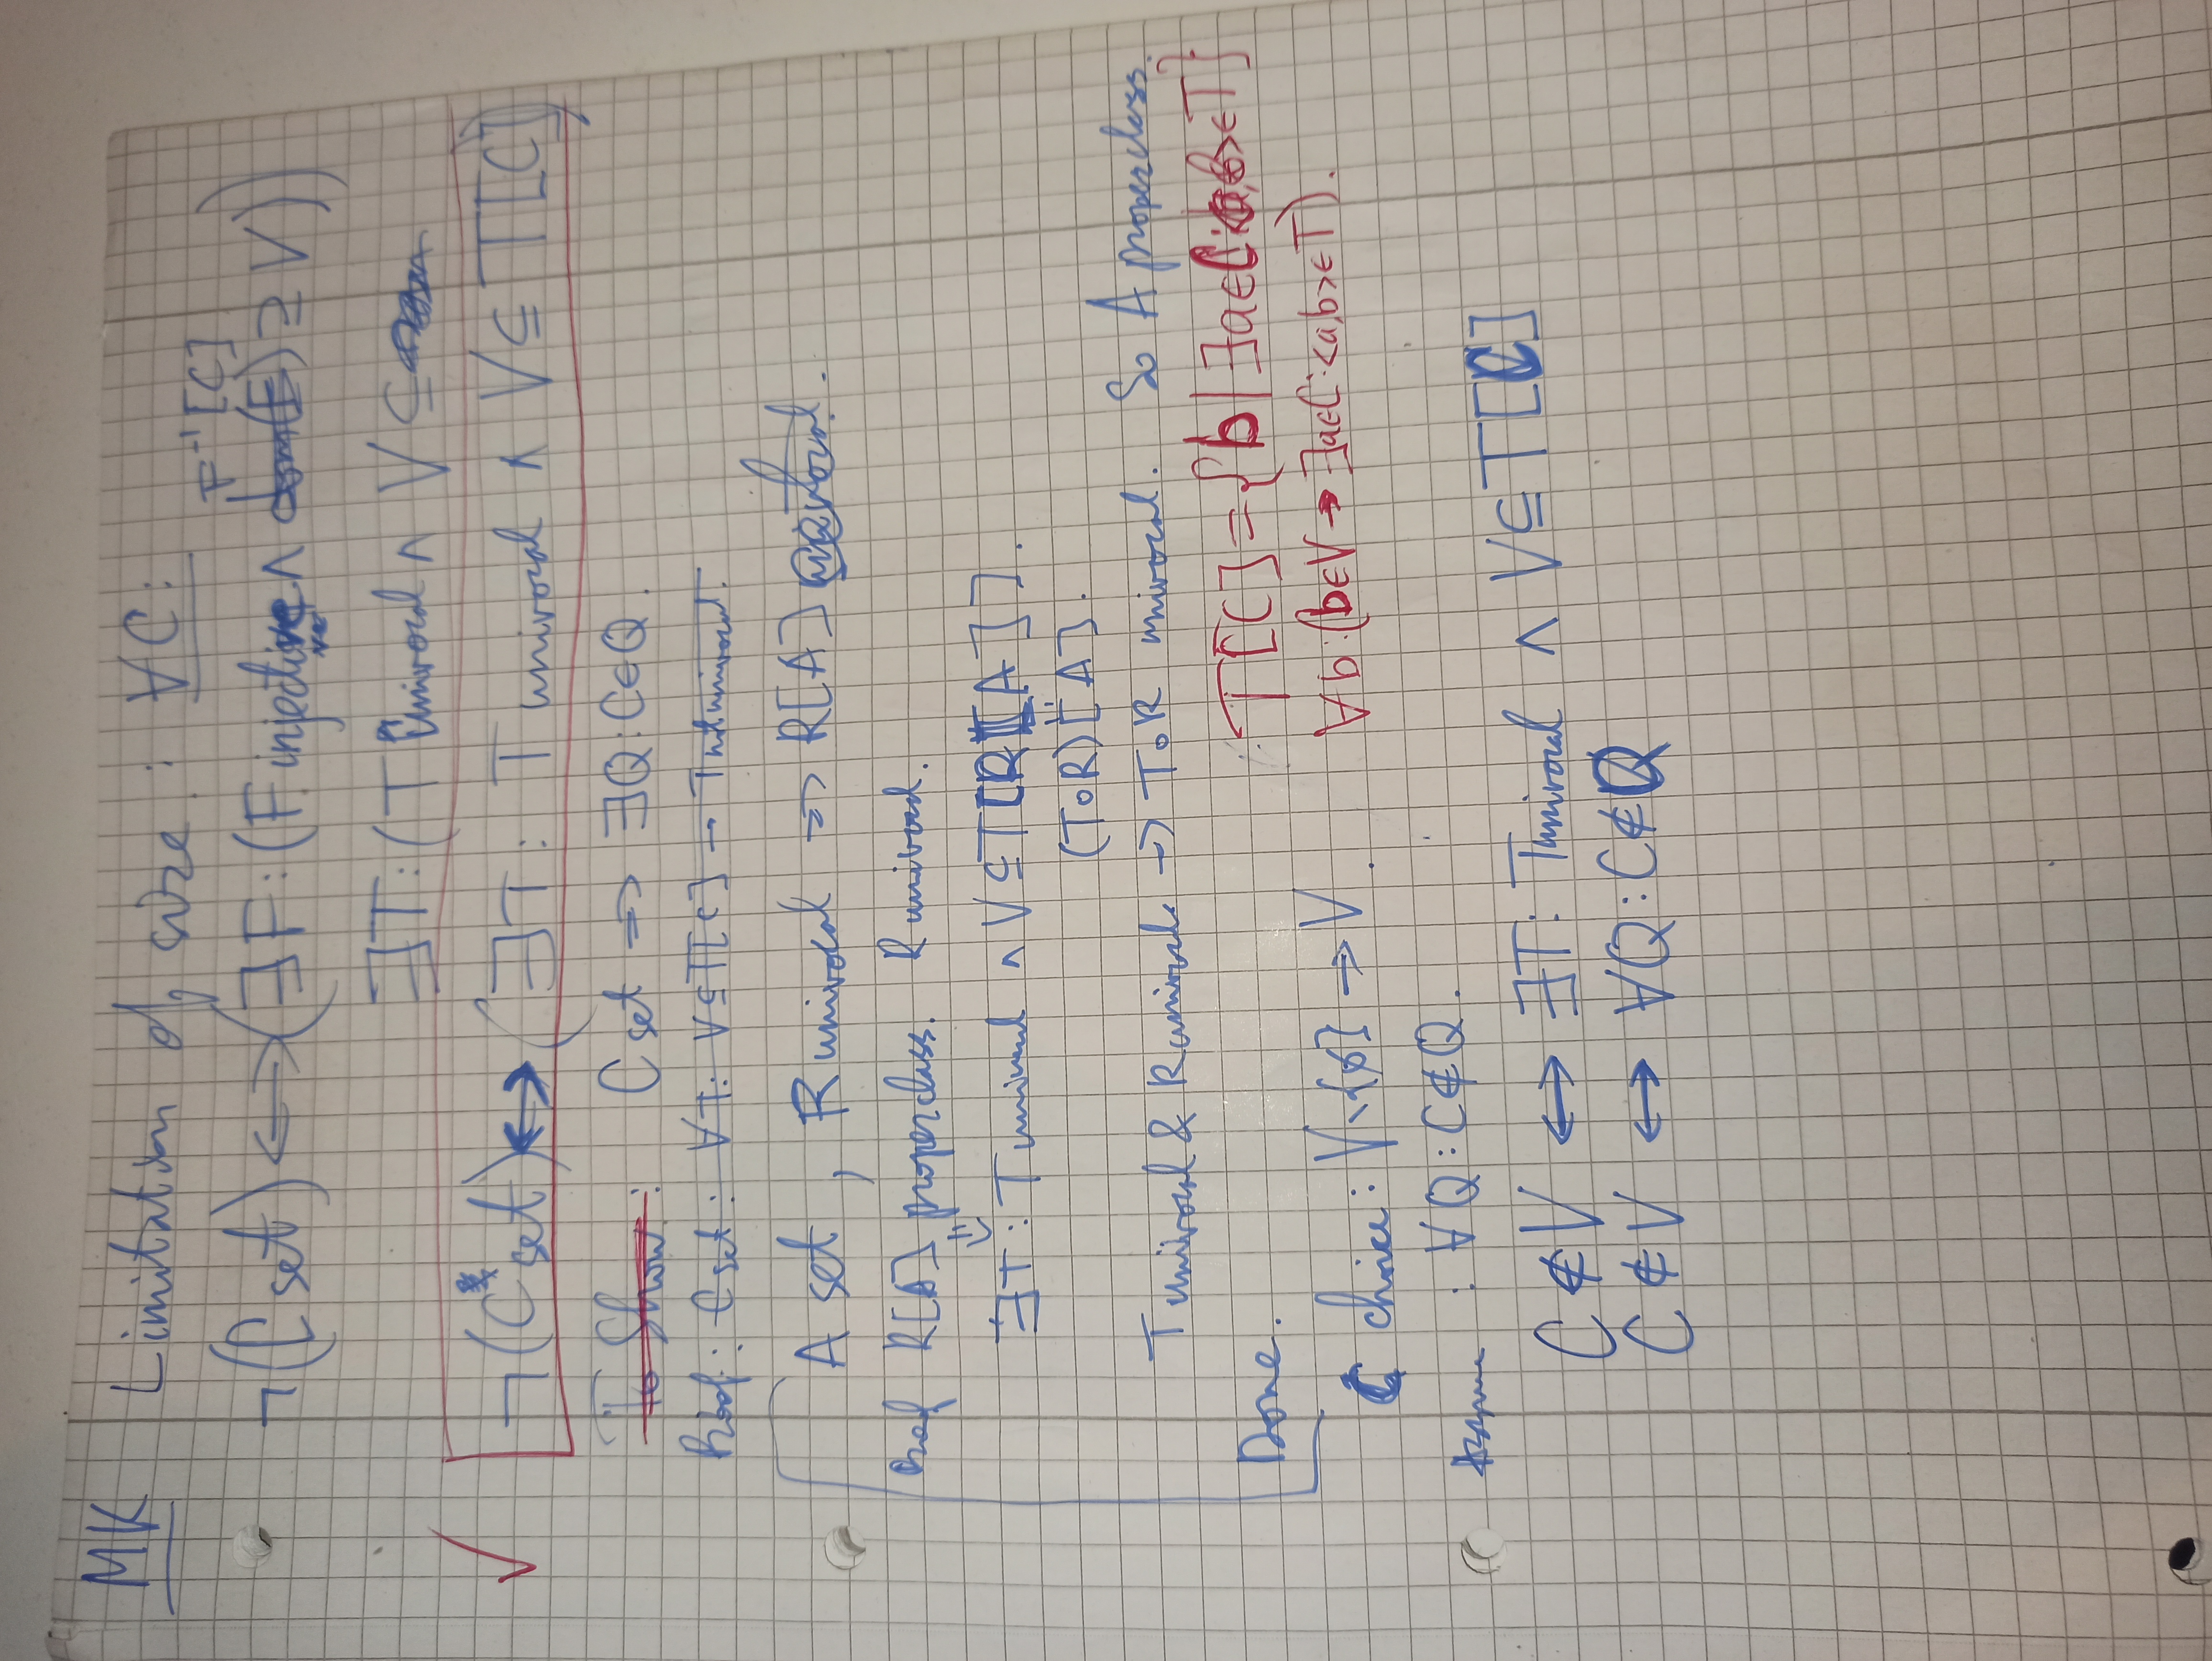
\includegraphics[angle=-90,origin=c,scale=0.1]{azriel_levy/1.jpg}\\
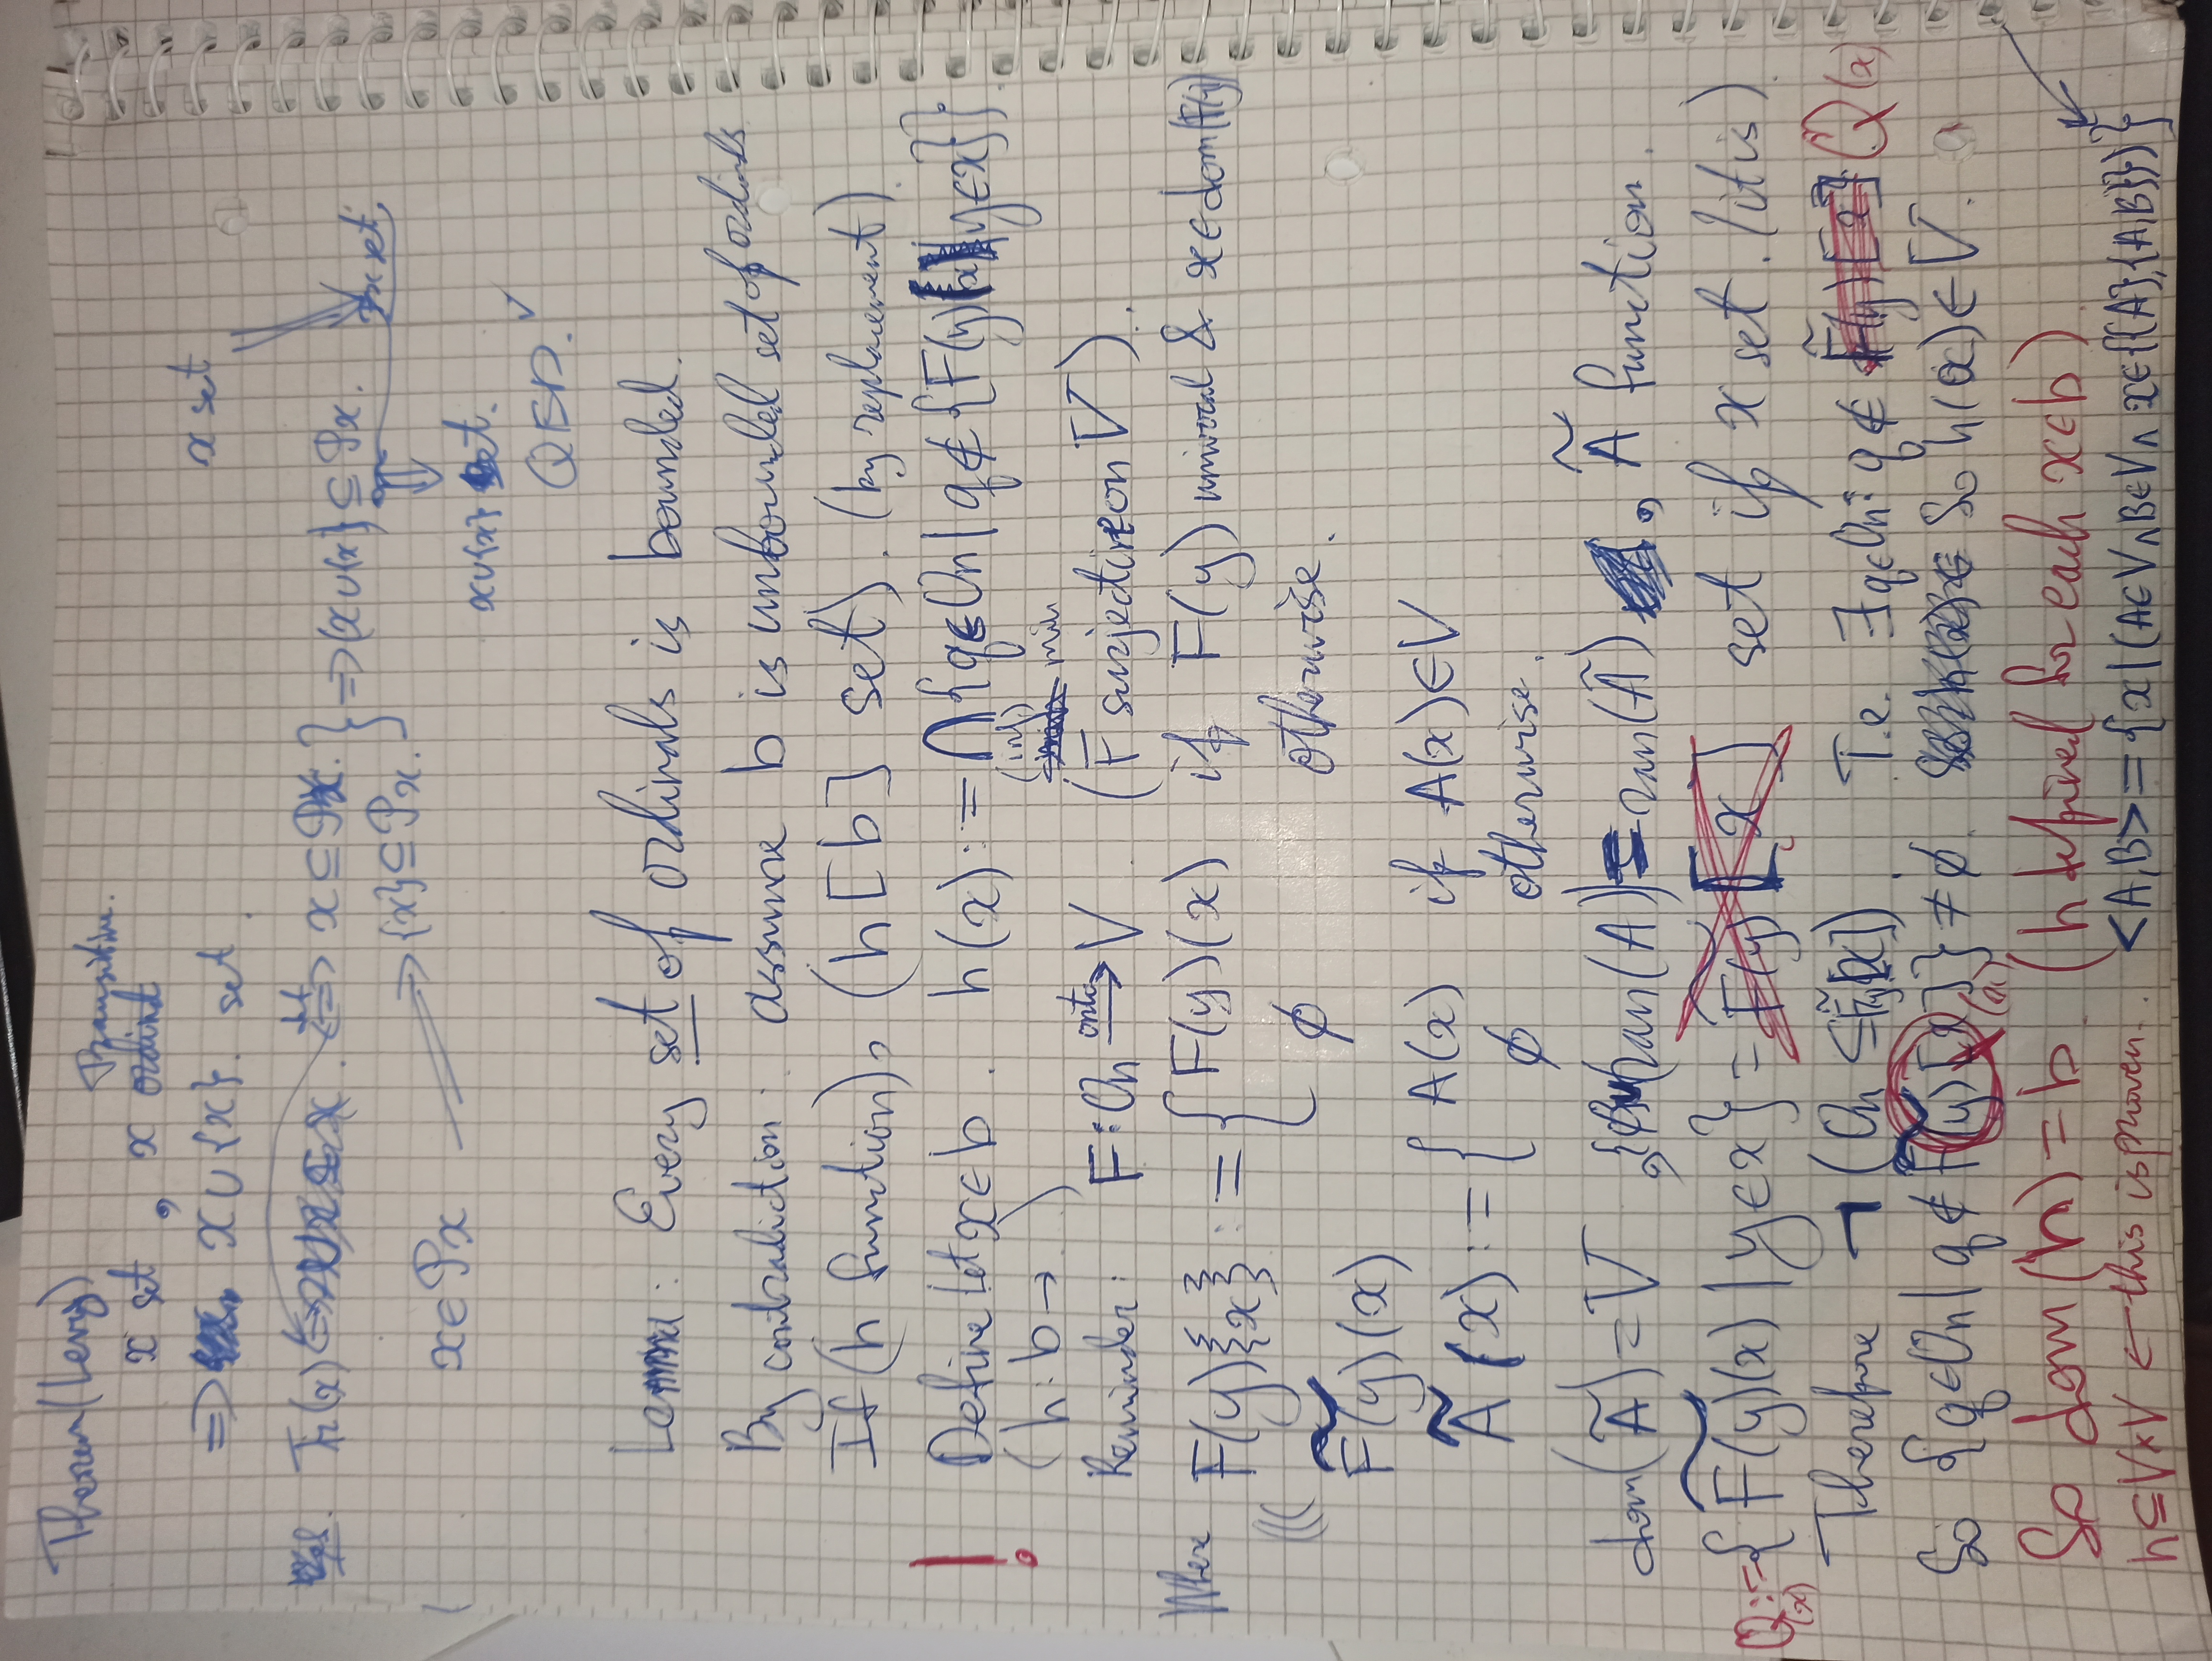
\includegraphics[angle=-90,origin=c,scale=0.1]{azriel_levy/2.jpg}\\
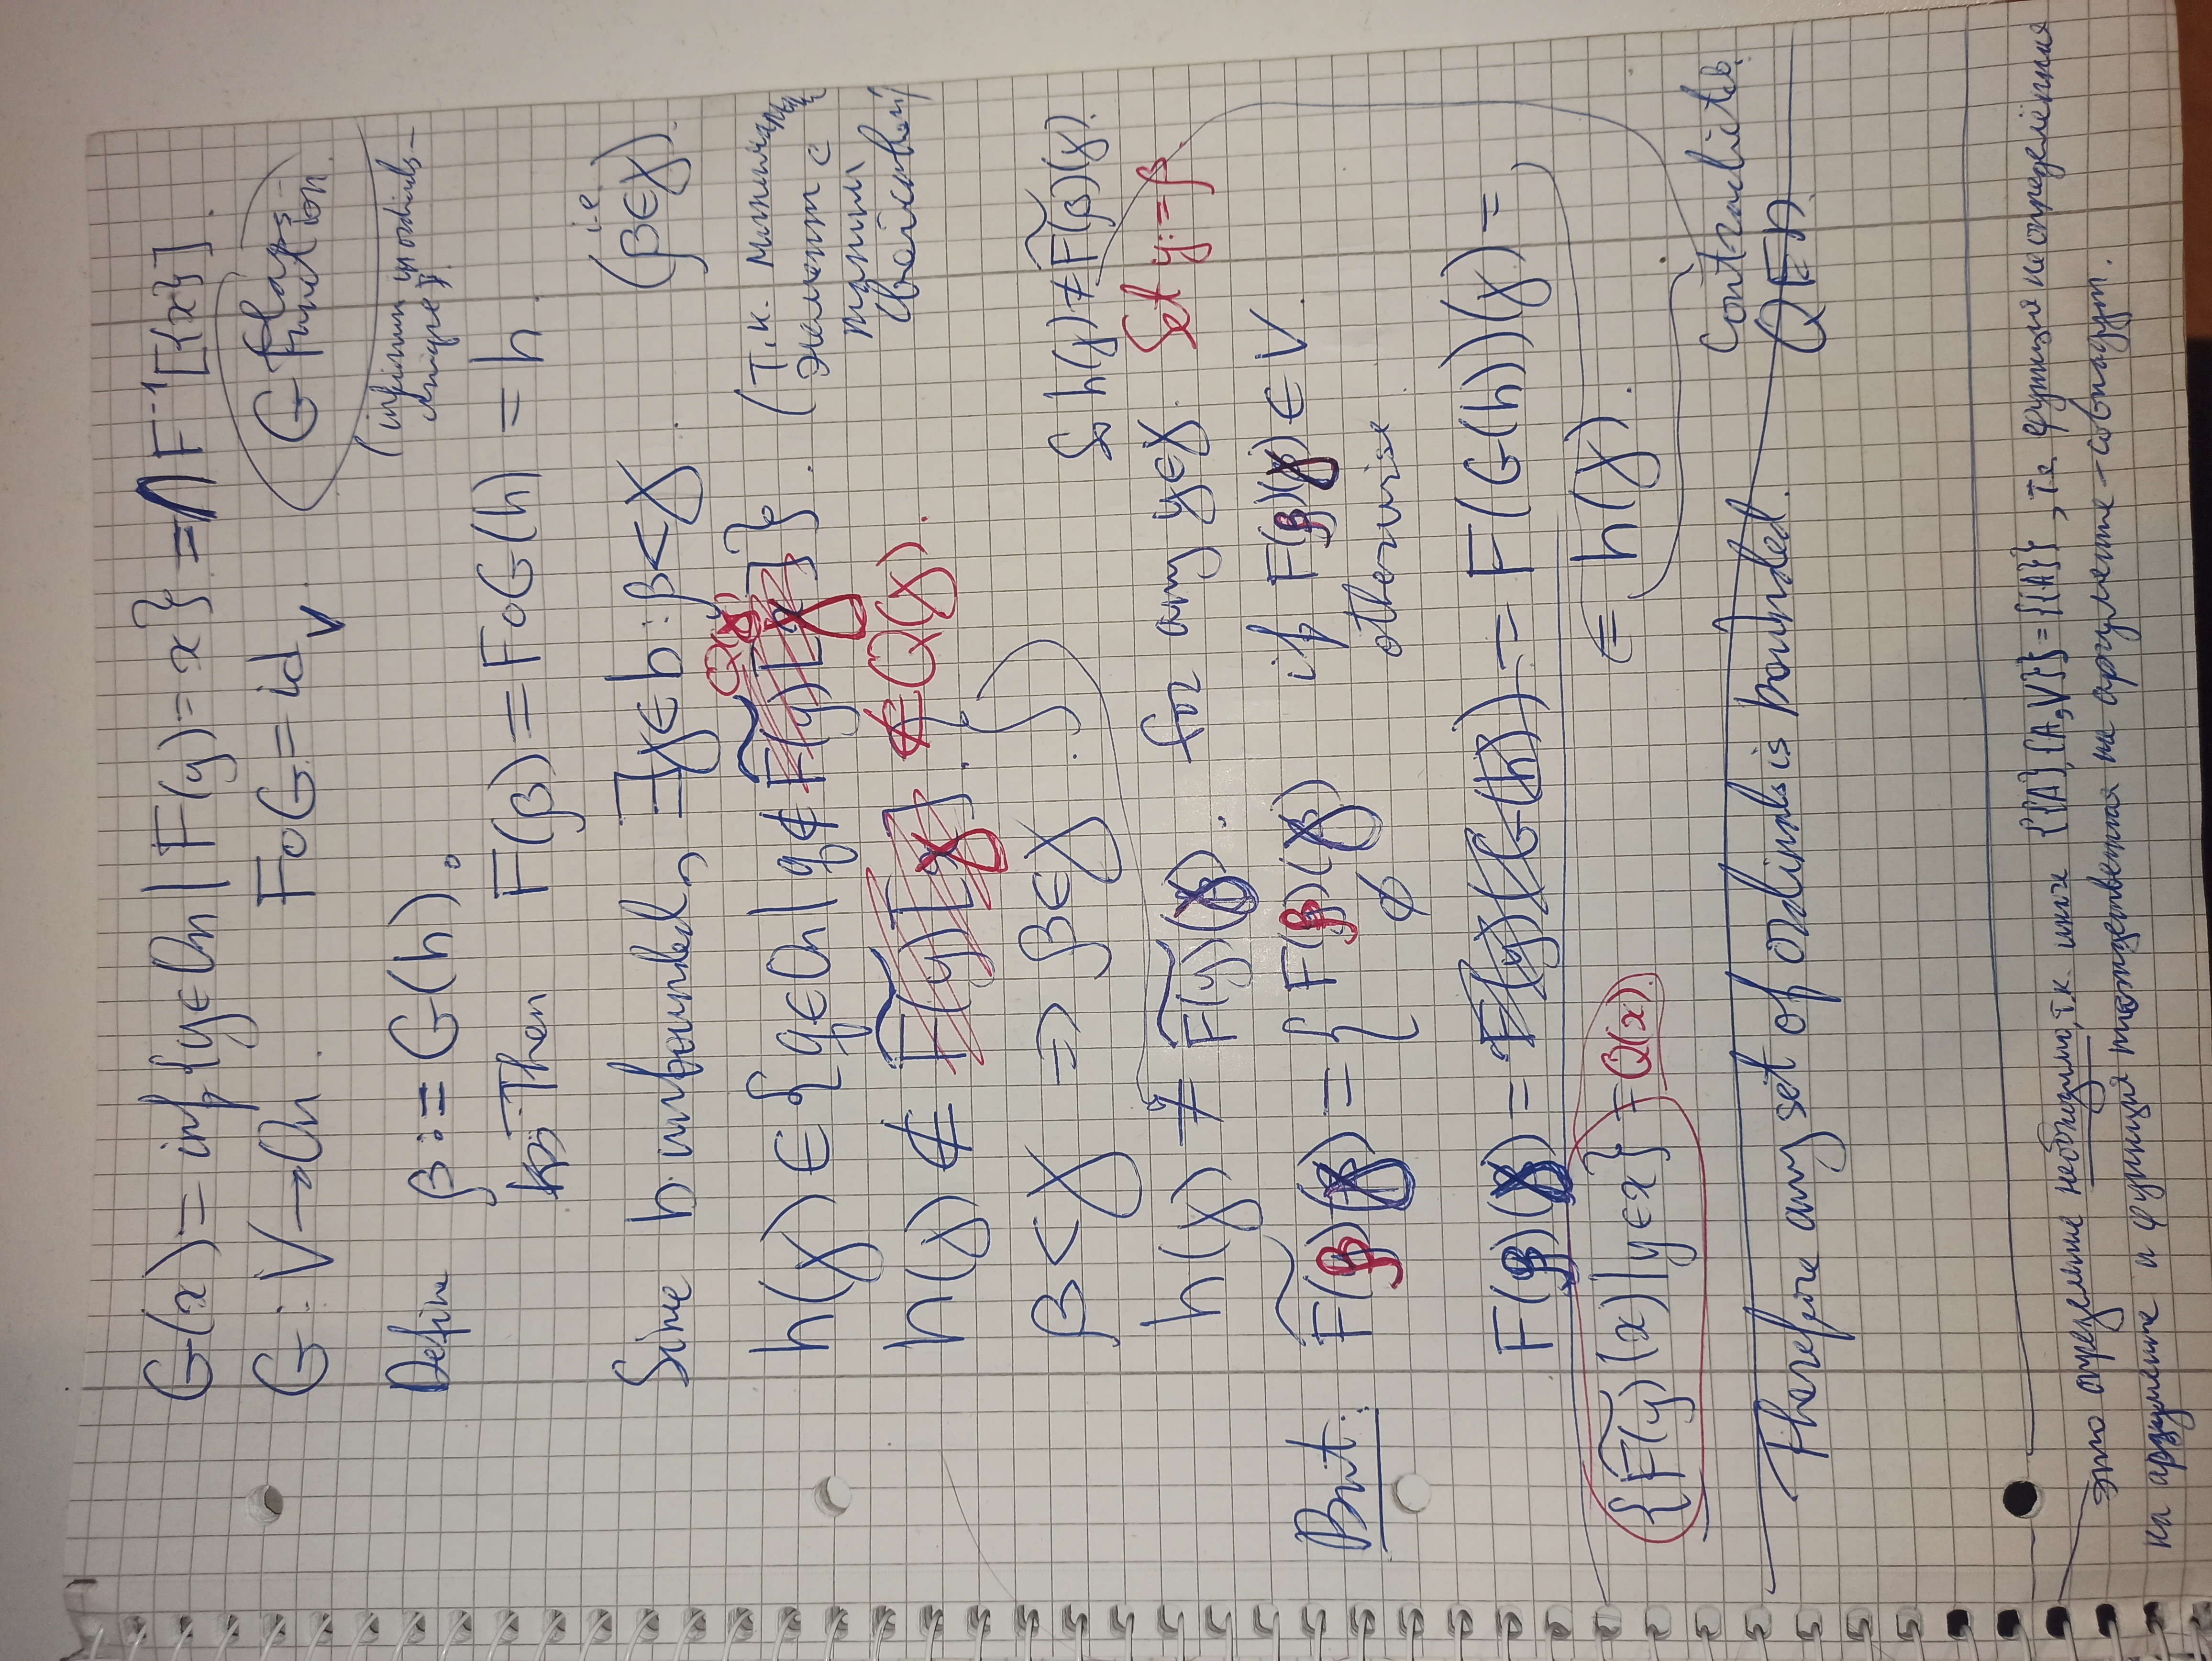
\includegraphics[angle=-90,origin=c,scale=0.1]{azriel_levy/3.jpg}\\
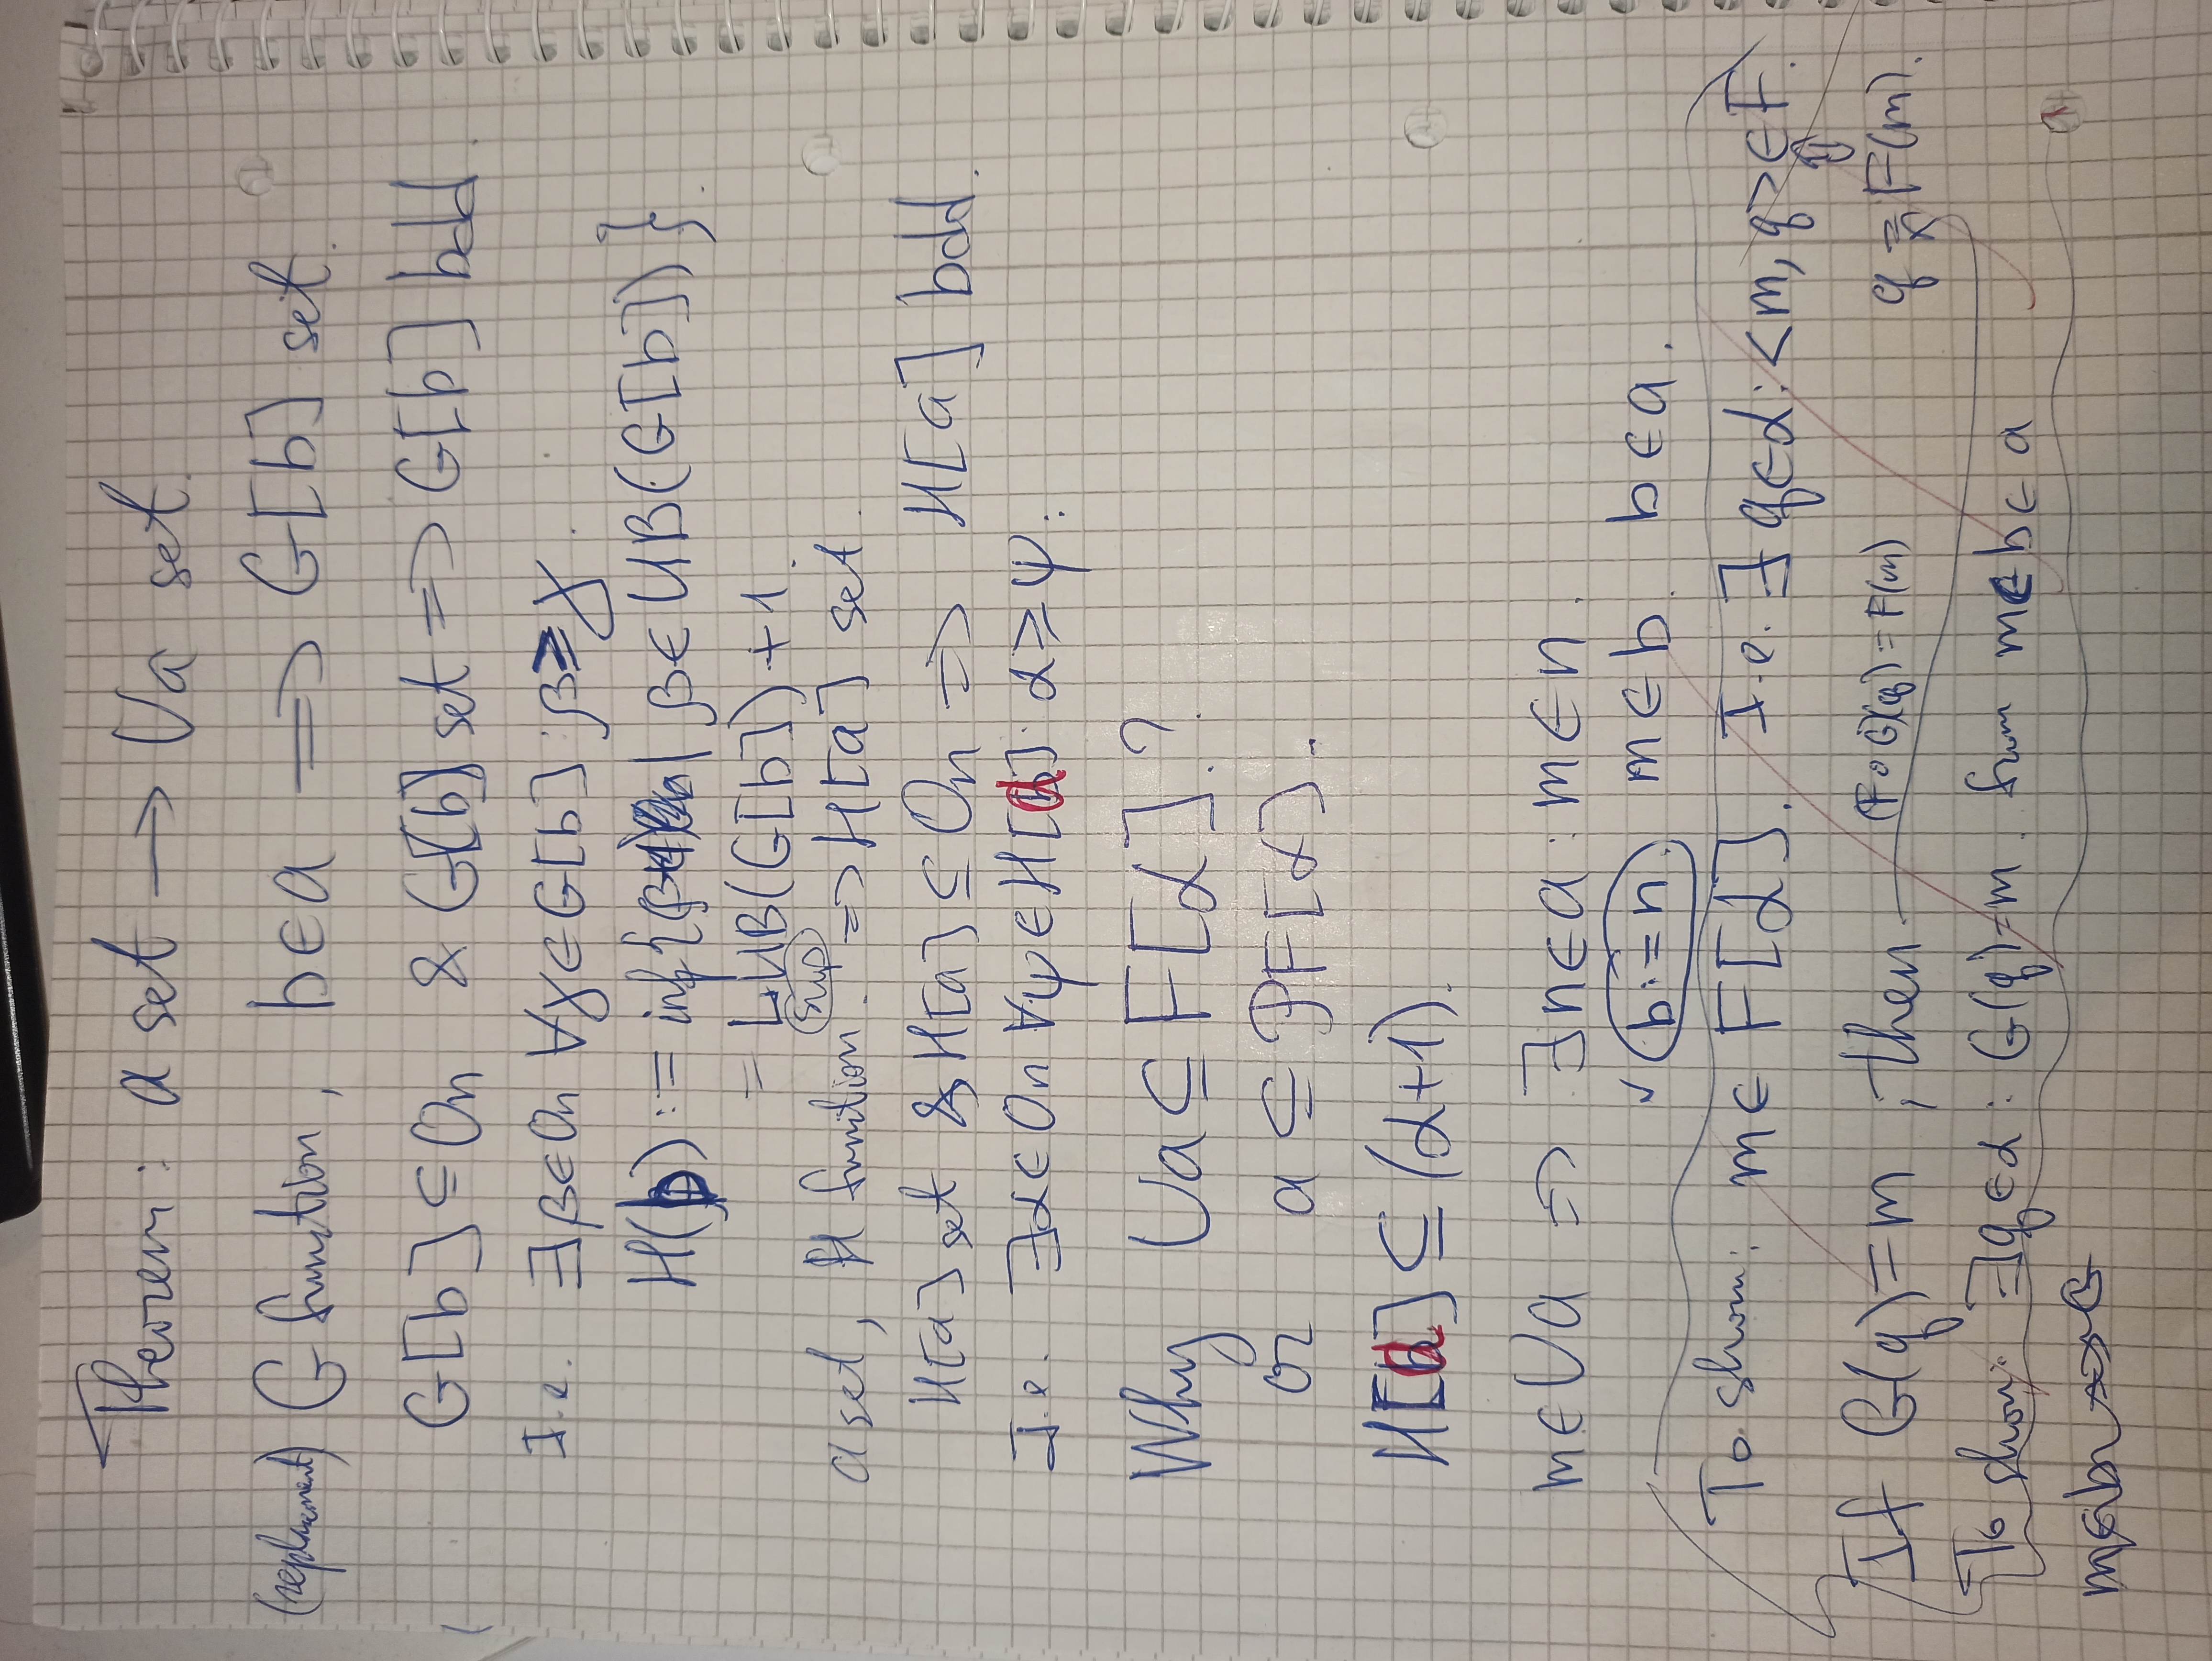
\includegraphics[angle=-90,origin=c,scale=0.1]{azriel_levy/4.jpg}\\
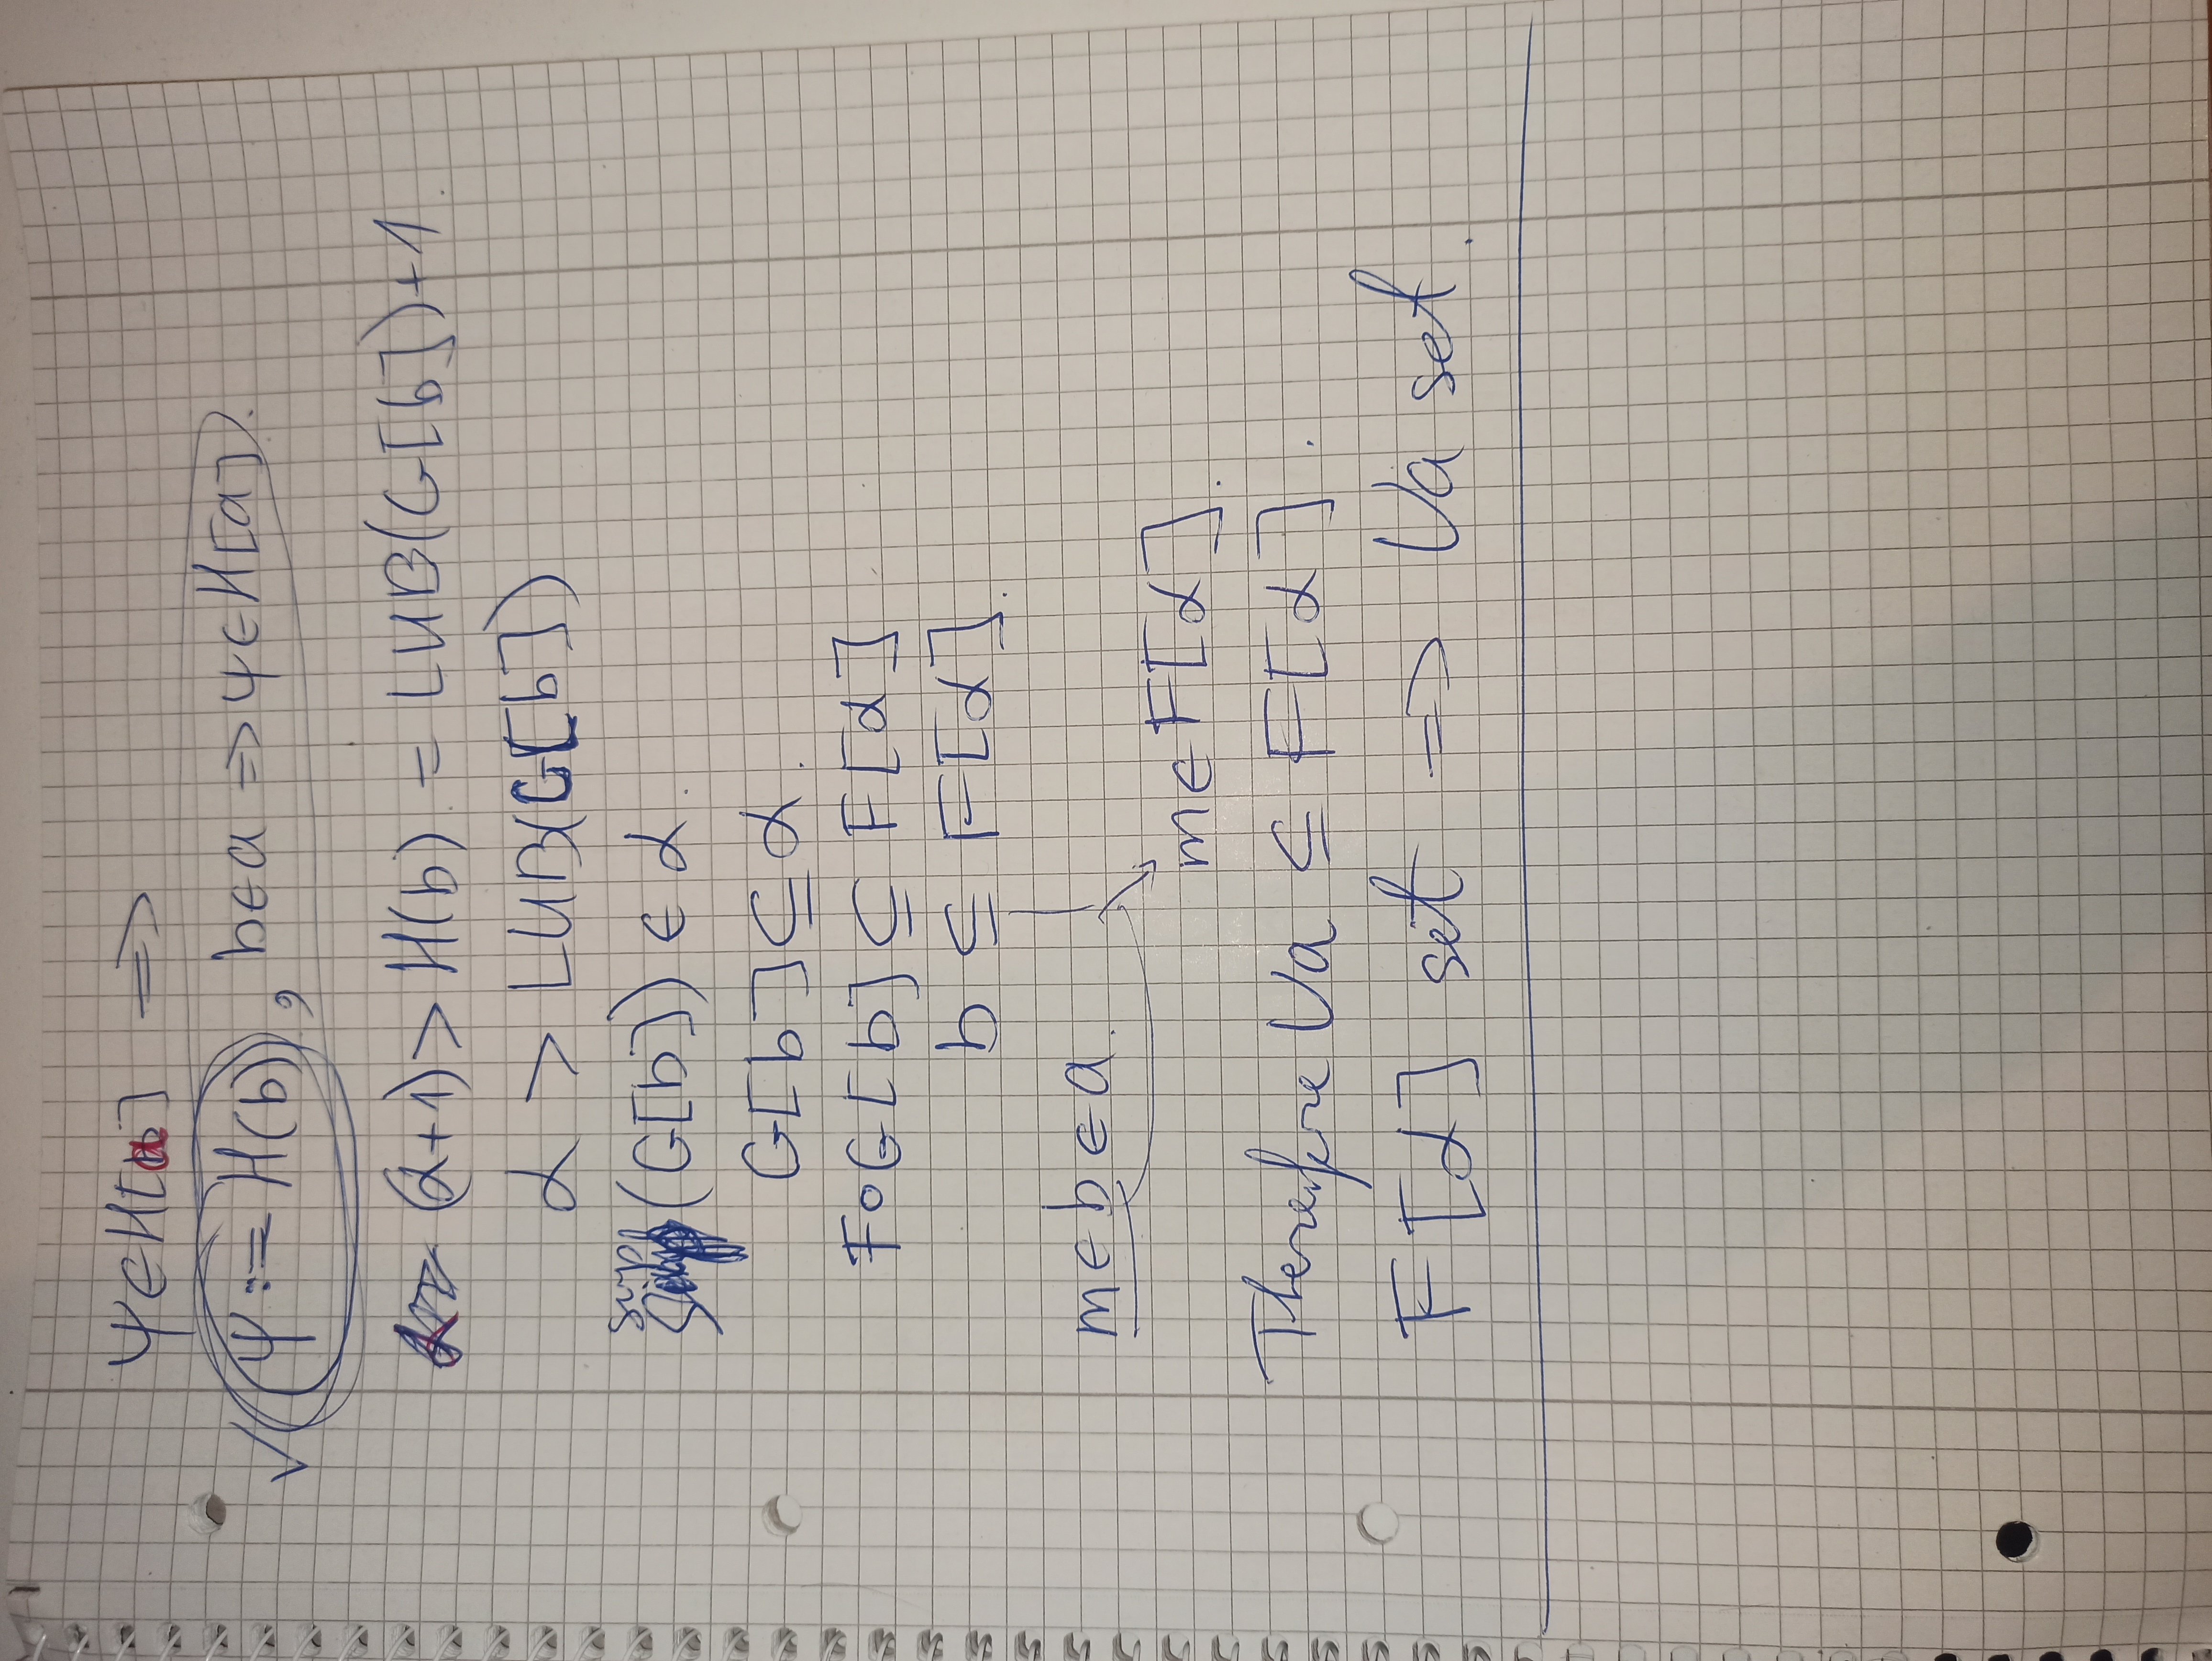
\includegraphics[angle=-90,origin=c,scale=0.1]{azriel_levy/5.jpg}\\
\fi
%\end{document}

\ifdefined\qwertyflag
\undef\qwertyflag
\end{document}
\fi
\pagebreak
\def\topic{Theorems related to Limitation of Size}
\ifdefined\MyHeaderIncluded
\else
\def\qwertyflag{true}

\ifdefined\MyHeaderIncluded

\else
  \newcommand{\foobar}{FooBar}
  \def\MyHeaderIncluded{true}
% if is till the end of the file

\documentclass[10pt,a4paper]{article}
\usepackage[utf8]{inputenc}
%\usepackage[german]{babel}
%\usepackage[cyrillic]{babel}
\usepackage[T1]{fontenc}
%\usepackage[T2A]{fontenc}
%\usepackage[english, russian]{babel}
\usepackage{amsmath}
\usepackage{amsfonts}
\usepackage{amssymb}
\usepackage{amsthm}
\usepackage{mathtools} %coloneqq

\usepackage{bussproofs} %

%\renewcommand{\thesubsection}{\arabic{subsection}}
%\newtheorem{thm}{Theorem}[section]
%\renewcommand{\thethm}{\arabic{subsection}.\arabic{thm}}

\usepackage{thmtools}
\usepackage{hyperref}
\hypersetup{
    colorlinks=true,
    linkcolor=blue,
    filecolor=magenta,      
    urlcolor=cyan,
    pdftitle={Overleaf Example},
    %pdfpagemode=FullScreen,
    }
%\usepackage{stix-type1}%\turnediota
\theoremstyle{definition}

\newtheorem{constructor}{Constructor}[section]
\newtheorem{iaxiom}{Axiom}
\newtheorem{axiom}{Axiom}
\newtheorem*{axiom*}{Axiom}
\newtheorem{definition}{Definition}[section]
\newtheorem*{definition*}{Definition}
\newtheorem{remark}{Remark}[section]
\newtheorem*{remark*}{Remark}
\newtheorem{recall}{Recall}[section]
\newtheorem*{recall*}{Recall}

\newtheorem{lemma}{Lemma}[section]
\newtheorem{theorem}{Theorem}[section]
\newtheorem*{theorem*}{Theorem}
\newtheorem{note}{Note}[section]
\usepackage{etoolbox}

%\newcommand*{\@Dashv}[2]{%
%  \reflectbox{$\m@th#1#2$}%
%}
\newcommand*{\separation}[3]{% 1)binder, 2)set, 3)condition
  \{#1\in #2: #3\}
}

% https://www.freecodecamp.org/news/simple-regex-tricks-for-beginners-3acb3fa257cb/
%  \\mathcal\{T\} |---> \topology
%  \\mathcal\{([^\}]*)\}   |--->  $1
\newcommand{\AND}{\ \ \&\ \ }
\newcommand{\any}{\mathrm{\ any}}
\newcommand{\borel}{\mathcal{B}}
\newcommand{\can}{\mathrm{can}}
\newcommand{\canonize}{\mathrm{canonize}}
\newcommand{\closure}{\mbox{cl}}
\newcommand{\complex}{\mathbb{C}}
\newcommand{\converges}{\longrightarrow}
\newcommand{\countable}{\mbox{\ countable}}
\newcommand{\ldefined}{\mbox{\ defined}}
\newcommand{\dom}{\mbox{dom}}
\newcommand{\Dom}{\mbox{Dom}}
\newcommand{\Done}{\noindent \textbf{Done.}\\}
\newcommand{\lexists}{\mbox{\ exists}}
\newcommand{\lforall}{\mbox{\ forall}}
\newcommand{\lunique}{\mbox{\ unique}}
\newcommand{\family}{\mathrm{\ family}}
\newcommand{\Fm}{\mathrm{Fm}}
\newcommand{\FuncSymb}{\mathrm{FuncSymb}}
\newcommand{\function}{\mathrm{\ function}}
\newcommand{\functional}{\mbox{\ functional}}
\newcommand{\IFF}{\ \Longleftrightarrow\ }
\renewcommand{\iff}{\ \longleftrightarrow\ }
\newcommand{\IMPLIES}{\ \Longrightarrow\ }
\renewcommand{\implies}{\ \longrightarrow\ }
\newcommand{\Inf}{\mathrm{Inf}}
\newcommand{\injective}{\mbox{\ injective}}
\newcommand{\injection}{\mbox{\ injection}}
\newcommand{\interior}{\mbox{int}}
\newcommand{\intersection}{\bigcap}
\newcommand{\isempty}{\mathrm{\ empty}}
\newcommand{\LB}{\mathrm{LB}}
\newcommand{\nghbset}{\mathcal{N}}
\newcommand{\nonempty}{\mathrm{\ nonempty}}
\newcommand{\Ord}{\mathrm{Ord}}
\newcommand{\power}{\mathcal{P}}
\newcommand{\pr}{\mathrm{pr}}
\newcommand{\fst}{\mathrm{fst}}
\newcommand{\snd}{\mathrm{snd}}
\newcommand{\PredSymb}{\mathrm{PredSymb}}
\newcommand{\Proof}{\noindent \textbf{Proof.}\\}
\newcommand{\ran}{\mathrm{ran}}
\newcommand{\Ran}{\mathrm{Ran}}
\newcommand{\real}{\mathbb{R}}
\newcommand{\relation}{\mathrm{\ relation}}
\newcommand{\set}{\mathrm{\ set}}
\newcommand{\singleton}{\mathrm{\ singleton}}
\newcommand{\semantics}{\mathrm{semantics}}
\newcommand{\semialgebra}{\mathcal{S}}
\newcommand{\Sup}{\mathrm{Sup}}
\newcommand{\surjective}{\mbox{\ surjective\ on\ }}
\newcommand{\Term}{\mathrm{Term}}
\newcommand{\Type}{\mathrm{Type}}
\newcommand{\topology}{\mathcal{T}}
\newcommand{\total}{\mbox{\ total\ on\ }}
\newcommand{\transitive}{\mathrm{\ transitive}}
\newcommand{\union}{\bigcup}
\newcommand{\lTrue}{\mathrm{True}}
\newcommand{\lFalse}{\mathrm{False}}
\newcommand{\lUncertain}{\mathrm{Uncertain}}
\newcommand{\lif}{\mathrm{if}}
\newcommand{\lthen}{\mathrm{then}}
\newcommand{\lelse}{\mathrm{else}}
\newcommand{\lexception}{\mathrm{exception}}
\newcommand{\lundef}{\mathrm{undef}}
\newcommand{\univocal}{\mathrm{\ univocal}}
\newcommand{\univocalat}{\mathrm{\ univocal\ at\ }}
\newcommand{\UB}{\mathrm{UB}}
\newcommand{\Un}{\mathcal{U}}
\newcommand{\Var}{\mathrm{Var}}

\newcommand{\notvarphi}{\phi}
\renewcommand{\phi}{\varphi}

\newcommand{\comment}[1]{\quad\mbox{(#1)}}
% local commands
%\preto\section{\undef\blipo} %etoolbox
\preto\subsection{\undef\blipo} %etoolbox
% https://tex.stackexchange.com/questions/105684/limit-macro-newcommand-scope-to-section
\usepackage{graphicx}
\usepackage{authblk}

\setlength\parindent{0pt} % whole doc of \noindent
\usepackage{soul}
%\usepackage{mathgl}

\fi % guard
\ifdefined\topic
\else
\def\topic{No Titel}
\fi
\title{\topic}
\author[1]{Georgy Dunaev}
\begin{document}
\maketitle
\fi
\section{Theorems Related to Limitation of Size}
\label{sec:limitation_of_size_theorems}



% This part is self-contained.
%\\\n%\\

The goal is to prove axiom of limitation of size using the small amount of usual axioms and simple definitions.

\begin{iaxiom}[Limitation of Size]
\[
(K\in V)
\iff
(|K| < |V|)
\]
\end{iaxiom}

Some equivalent(in normal context) statements:
\[
(K\in V)
\iff
(K\in V)
(|K| \subsetneq |V|)
\]
\[
(K\in V)
\iff
(K\in V)
(|K| \neq |V|)
\]
because $|V|=\On$.


\subsection{Proof of the Limitation of Size via Other Axioms}
\label{subsec:limitation_of_size_proof}
We want to prove the following statement:
\[
(K \in V) \iff (|K| \neq |V|)
\]

Firstly, we will prove some lemmas:



\begin{lemma}[First Part of the Limitation of Size Statement]
\label{lem:limitation_of_size_first_part}
\[
(K \in V) \implies (|K| \neq |V|)
\]
\end{lemma}
\begin{proof}
Assume $(K \in V)$.\\
By our axiom, since $(K \in V)$ we have $(|K| \in \On)$.\\
By previous lemmas we have $|V|=\On$ and $\On\notin\On$.\\
From these three statements we deduce that $|K| \neq |V|$.\\
\Done

\begin{lemma}[Second Part of the Limitation of Size Statement]
\label{lem:limitation_of_size_second_part}
\[
(|K| \neq |V|) \implies (K \in V)
\]
\end{lemma}
\begin{proof}
Assume $(|K| \neq |V|)$.\\
We know that $(|V|=\On)$, so $(|K| \neq \On)$.\\
Recalling the definition:
$|K|\ceq \On \cap \bigcap \cc{a\in\On}{K\preccurlyeq a}$.\\
Now we have that 
there exists some $m \in \On$, which is not in $\bigcap \cc{a\in\On}{K\preccurlyeq a}$. (vice versa situation is not possible since any non--empty intersection of subclasses of $\On$ is subclass of $\On$)\\
...
\Done
\pagebreak
\section{Properties Preserved by Intersections of Universes}
\label{sec:properties_preserved_intersections}

\iffalse
\section{Proposed foundations which axioms consist only of positive properties}
\begin{lstlisting}
\input{./Coq/positive_foundations.v}
\end{lstlisting}
% Risky!
\fi
\ifdefined\qwertyflag
\undef\qwertyflag
\end{document}
\fi
\pagebreak
% 100_class_theory.tex -- Class Theory Overview.
% Ticket 7335: cosmetic cleanup (typography, normalized blank-line spacing,
% consistent section formatting). Content is semantically unchanged.
% Author: opencode-go/glm-5.3-flash (Capability Tier 2)
\section{Class Theory Overview}

This section provides an overview of class theory, including definitions, axioms, and fundamental concepts. It serves as a foundational reference for understanding the structure and properties of classes in set theory.

\subsection{Definitions}

In class theory, a class is a collection of sets that is too large to be considered a set. Classes are often defined using a property that their members satisfy. For example, the class of all sets is a proper class, as it is too large to be a set.

\subsection{Axioms}

Class theory is based on a set of axioms that define the properties of classes and sets. The most common axioms in class theory include the Axiom of Extensionality, the Axiom of Regularity, and the Axiom of Choice.

\pagebreak
\def\topic{Evaluation}
\ifdefined\MyHeaderIncluded
\else
\def\qwertyflag{true}

\ifdefined\MyHeaderIncluded

\else
  \newcommand{\foobar}{FooBar}
  \def\MyHeaderIncluded{true}
% if is till the end of the file

\documentclass[10pt,a4paper]{article}
\usepackage[utf8]{inputenc}
%\usepackage[german]{babel}
%\usepackage[cyrillic]{babel}
\usepackage[T1]{fontenc}
%\usepackage[T2A]{fontenc}
%\usepackage[english, russian]{babel}
\usepackage{amsmath}
\usepackage{amsfonts}
\usepackage{amssymb}
\usepackage{amsthm}
\usepackage{mathtools} %coloneqq

\usepackage{bussproofs} %

%\renewcommand{\thesubsection}{\arabic{subsection}}
%\newtheorem{thm}{Theorem}[section]
%\renewcommand{\thethm}{\arabic{subsection}.\arabic{thm}}

\usepackage{thmtools}
\usepackage{hyperref}
\hypersetup{
    colorlinks=true,
    linkcolor=blue,
    filecolor=magenta,      
    urlcolor=cyan,
    pdftitle={Overleaf Example},
    %pdfpagemode=FullScreen,
    }
%\usepackage{stix-type1}%\turnediota
\theoremstyle{definition}

\newtheorem{constructor}{Constructor}[section]
\newtheorem{iaxiom}{Axiom}
\newtheorem{axiom}{Axiom}
\newtheorem*{axiom*}{Axiom}
\newtheorem{definition}{Definition}[section]
\newtheorem*{definition*}{Definition}
\newtheorem{remark}{Remark}[section]
\newtheorem*{remark*}{Remark}
\newtheorem{recall}{Recall}[section]
\newtheorem*{recall*}{Recall}

\newtheorem{lemma}{Lemma}[section]
\newtheorem{theorem}{Theorem}[section]
\newtheorem*{theorem*}{Theorem}
\newtheorem{note}{Note}[section]
\usepackage{etoolbox}

%\newcommand*{\@Dashv}[2]{%
%  \reflectbox{$\m@th#1#2$}%
%}
\newcommand*{\separation}[3]{% 1)binder, 2)set, 3)condition
  \{#1\in #2: #3\}
}

% https://www.freecodecamp.org/news/simple-regex-tricks-for-beginners-3acb3fa257cb/
%  \\mathcal\{T\} |---> \topology
%  \\mathcal\{([^\}]*)\}   |--->  $1
\newcommand{\AND}{\ \ \&\ \ }
\newcommand{\any}{\mathrm{\ any}}
\newcommand{\borel}{\mathcal{B}}
\newcommand{\can}{\mathrm{can}}
\newcommand{\canonize}{\mathrm{canonize}}
\newcommand{\closure}{\mbox{cl}}
\newcommand{\complex}{\mathbb{C}}
\newcommand{\converges}{\longrightarrow}
\newcommand{\countable}{\mbox{\ countable}}
\newcommand{\ldefined}{\mbox{\ defined}}
\newcommand{\dom}{\mbox{dom}}
\newcommand{\Dom}{\mbox{Dom}}
\newcommand{\Done}{\noindent \textbf{Done.}\\}
\newcommand{\lexists}{\mbox{\ exists}}
\newcommand{\lforall}{\mbox{\ forall}}
\newcommand{\lunique}{\mbox{\ unique}}
\newcommand{\family}{\mathrm{\ family}}
\newcommand{\Fm}{\mathrm{Fm}}
\newcommand{\FuncSymb}{\mathrm{FuncSymb}}
\newcommand{\function}{\mathrm{\ function}}
\newcommand{\functional}{\mbox{\ functional}}
\newcommand{\IFF}{\ \Longleftrightarrow\ }
\renewcommand{\iff}{\ \longleftrightarrow\ }
\newcommand{\IMPLIES}{\ \Longrightarrow\ }
\renewcommand{\implies}{\ \longrightarrow\ }
\newcommand{\Inf}{\mathrm{Inf}}
\newcommand{\injective}{\mbox{\ injective}}
\newcommand{\injection}{\mbox{\ injection}}
\newcommand{\interior}{\mbox{int}}
\newcommand{\intersection}{\bigcap}
\newcommand{\isempty}{\mathrm{\ empty}}
\newcommand{\LB}{\mathrm{LB}}
\newcommand{\nghbset}{\mathcal{N}}
\newcommand{\nonempty}{\mathrm{\ nonempty}}
\newcommand{\Ord}{\mathrm{Ord}}
\newcommand{\power}{\mathcal{P}}
\newcommand{\pr}{\mathrm{pr}}
\newcommand{\fst}{\mathrm{fst}}
\newcommand{\snd}{\mathrm{snd}}
\newcommand{\PredSymb}{\mathrm{PredSymb}}
\newcommand{\Proof}{\noindent \textbf{Proof.}\\}
\newcommand{\ran}{\mathrm{ran}}
\newcommand{\Ran}{\mathrm{Ran}}
\newcommand{\real}{\mathbb{R}}
\newcommand{\relation}{\mathrm{\ relation}}
\newcommand{\set}{\mathrm{\ set}}
\newcommand{\singleton}{\mathrm{\ singleton}}
\newcommand{\semantics}{\mathrm{semantics}}
\newcommand{\semialgebra}{\mathcal{S}}
\newcommand{\Sup}{\mathrm{Sup}}
\newcommand{\surjective}{\mbox{\ surjective\ on\ }}
\newcommand{\Term}{\mathrm{Term}}
\newcommand{\Type}{\mathrm{Type}}
\newcommand{\topology}{\mathcal{T}}
\newcommand{\total}{\mbox{\ total\ on\ }}
\newcommand{\transitive}{\mathrm{\ transitive}}
\newcommand{\union}{\bigcup}
\newcommand{\lTrue}{\mathrm{True}}
\newcommand{\lFalse}{\mathrm{False}}
\newcommand{\lUncertain}{\mathrm{Uncertain}}
\newcommand{\lif}{\mathrm{if}}
\newcommand{\lthen}{\mathrm{then}}
\newcommand{\lelse}{\mathrm{else}}
\newcommand{\lexception}{\mathrm{exception}}
\newcommand{\lundef}{\mathrm{undef}}
\newcommand{\univocal}{\mathrm{\ univocal}}
\newcommand{\univocalat}{\mathrm{\ univocal\ at\ }}
\newcommand{\UB}{\mathrm{UB}}
\newcommand{\Un}{\mathcal{U}}
\newcommand{\Var}{\mathrm{Var}}

\newcommand{\notvarphi}{\phi}
\renewcommand{\phi}{\varphi}

\newcommand{\comment}[1]{\quad\mbox{(#1)}}
% local commands
%\preto\section{\undef\blipo} %etoolbox
\preto\subsection{\undef\blipo} %etoolbox
% https://tex.stackexchange.com/questions/105684/limit-macro-newcommand-scope-to-section
\usepackage{graphicx}
\usepackage{authblk}

\setlength\parindent{0pt} % whole doc of \noindent
\usepackage{soul}
%\usepackage{mathgl}

\fi % guard
\ifdefined\topic
\else
\def\topic{No Titel}
\fi
\title{\topic}
\author[1]{Georgy Dunaev}
\begin{document}
\maketitle
\fi
\section{Evaluation in context of pluralistic semantic}
\begin{definition}[value]
\[
F(x) :\simeq \left(\lif ((F\family)\land(x \in \dom(F)))\ \lthen\ \union\cc{s}{(x,s)\in F}\ \lelse\ \lundef\ \lexception\_\lelse\ \lundef\right)
\]
\end{definition}
\subsection{Value} % of a function.
Definition of the value of the function:
%(in the context of 3--valued logic)
\begin{definition}[semi--equality]
\[
I_{\Fm}(s\approx t) :\IFF 
\]
%(((s \ldefined)\lor(t \ldefined)) \implies (s=t))
\end{definition}

\begin{definition}[equality]?
%\[
%(I^\loc,w_\Fm(s = t)=\ltrue) \IFF \forall \left(v:\prod_{x:Var}w(x)\right),\ I_\Term^{\loc,v}%(t)=I_\Term^{\loc,v}(s)
%\]
%\[
%(I^glob_\Fm(s = t)=\lTrue) \IFF \forall (w:\Var\to\power\Un\setminus\{\emptyclass\} \forall (v:\prod_{x:Var}w(x)),\ I_\Term^{\loc,v}(t)=I_\Term^{\loc,v}(s)
%\]
%(((s \ldefined)\lor(t \ldefined)) \implies (s=t))
\end{definition}

\begin{definition}[quasi--equality](Note: it is good for semantics with partial functions, not the two level set--semantics i use.)
\[
(s\simeq t) :\IFF (((s \ldefined)\lor(t \ldefined)) \implies (s=t))
\]
\end{definition}

\begin{definition}[underdefined class](Note: be careful, since not every undefined class is underdefined, some are overdefined in various ways, so not even semantically equal to eachother.)
\[
\lundef :\simeq (\varepsilon x,\ \bot)
\]
\end{definition}
What if $\varphi$ is assigned with $U$ (i.e. it is assigned with the "uncertain" truth value)?\\
If $(I(\varphi)=U)$, then 
\[
(I((\lif\ \varphi\ \lthen\ t_1\ \lelse\ t_2))=I(\lundef))
\]
should follow.\\
Btw, $I(\lundef)=\emptyclass$.\\
\pagebreak

\subsection{Some simple theorems about classes}
\begin{definition}[some syntactic sugar]
\[
(x\ \mbox{any}) :\iff \top
\]
Context: (x:Var)
%Side condition:\\
%Term $x$ is a variable.
\end{definition}

\begin{definition}[semi--singleton]
\[
(s\ \mbox{ss}) :\iff (!y,\ y\in s)
\]
Side condition:\\
Variable $y$ is not in free variables of term $s$.
\end{definition}

\begin{definition}[semi--singleton subset relation]
\[
(s\ \mbox{sss}\ t) :\iff ((s\ \mbox{ss})\land(s\subseteq t))
\]
\end{definition}

\begin{definition}[function constructor]
\[
(\lambda x,\ t) \ceq \cc{(x,t)}{(x\ \mbox{any})}
\]
Context: ($x$:Var) ($t$:Term)\\
Comment: Term $t$ can contain $x$ as a free variable.\\
Side conditions:\\ 
(variable $x$ is bound by class collection in r.h.s)\\
(variable $x$ is bound by lambda abstraction in l.h.s)\\
%No side conditions.
\end{definition}

\begin{definition}[family constructor]
\[
(\Lambda x,\ t) \ceq \cc{(x,s)}{(s\ \mbox{sss}\ t), x\ \mbox{any}}
\]
% s is a bound variable
Term $t$ can contain $x$ as a free variable.\\
Side conditions:\\
Variables x and s are different.\\ %it should be a normal convention for any definition.
Variable $s$ is not in free variables of $t$.\\
As term $s$ can contain $x$ as a free variable.\\
\end{definition}

\begin{definition*}[LOCAL definition of a value of a function, value of a family, for the next theorem]
\[
f(x) \ceq \bigcup \cc{s}{(x,s)\in f}
\]
\end{definition*}
% \coloneqq
% \vcentcolon = 

\begin{theorem}[evaluation of a function]
Context:\\
(x:Var)(t:Term)(z:Term)
\[
(z\set) \land (t[z/x]\set) \implies
\]
\[
(\lambda x,\ t)(z) = t[z/x]
\]
\end{theorem}
\Proof
To prove the equality, we use set extensionality and MP.
\[
((\lambda x,\ t)(z) \subseteq t[z/x] )
\land
((\lambda x,\ t)(z) \supseteq t[z/x] )
\implies
((\lambda x,\ t)(z) = t[z/x] )
\]
($\subseteq$)\\
Assume 
\[
q\in (\lambda x,\ t)(z)
\]
By definition of $-(-)$ (evaluation),
\[
q\in\union \cc{b}{(z,b)\in(\lambda x,\ t)}.
\]
By destruction of the union,
\[
(\exists s\in \cc{b}{(z,b)\in(\lambda x,\ t)},\ (q\in s)).
\]
Note for the following step: since variable b has no free occurences in t, $t[s/b]=t$.
\[
s\in \cc{b}{(z,b)\in(\lambda x,\ t)}
\IMPLIES
(s\set) \& ((z,s)\in(\lambda x,\ t))
\]
By definition of $\lambda$,
\[
(z,s)\in(\lambda x,\ t)
\IMPLIES
(z,s)\in \cc{(x,t)}{\top}
\]
Unfolding the notation:
\[
(z,s)\in \cc{(x,t)}{\top}
\IMPLIES
(z,s)\in \cc{w}{\exists x,\ w = (x,t) \land \top}
\]

\[
(z,s)\in \cc{w}{\exists x,\ w = (x,t) \land \top}
\IMPLIES
\exists x,\ (z,s) = (x,t) \land \top
\]
Notes: w is free in t, w is different from x. Since otherwise we would write $(x[(z,s)/w],t[(z,s)/w])$.

Take such x. By defining property of ordered pairs,
\[
(z,s) = (x,t)
\IMPLIES
(z=x) \& (s=t)
\]
\[
(q\in s)\& (s=t)
\IMPLIES
q\in t
\]
\[
z=x
\IMPLIES
t[z/x]=t
\]
Therefore
\[
(q\in t) \& (t[z/x]=t)
\IMPLIES
(q \in t[z/x])
\]
\ \\
\ \\
($\supseteq$)\\
Assume $(q \in t[z/x])$.\\
Let $s\ceq t[z/x]$. Then $(q\in s)$.\\
Goal1:$(z,s)\in(\lambda x,\ t)$.\\
\[
x[z/x]=z
\]
\[
(z,t[z/x]) = (x[z/x],t[z/x])=(x,t)[z/x]
\]
Goal1: $(x,t)[z/x]\in\cc{(x,t)}{(x\mbox{ any})}$\\
Goal2: $\exists x,\ (x,t)=((x,t)[z/x])$\\
$x\ceq z$\\
There are no free occurencies of $x$ in $((x,t)[z/x])$, because of the substitution.\\
$c\ceq ((x,t)[z/x])$\\
\[
(((x,t)[z/x])=c)\implies\exists x,\ (x,t)=c
\]
Goal' is done.\\

From the premise, $(x,t)[z/x]$ is a set.\\
Therefore Goal1 is proven.\\
So $(x,t)[z/x]\in (\lambda x,\ t)$.\\
So $(z,t[z/x])\in (\lambda x,\ t)$.\\
So $t[z/x]\in \cc{b}{(z,b)\in(\lambda x,\ t)}$.\\
Since $(q \in t[z/x])$, we also have
\[
q\in \bigcup \cc{b}{(z,b)\in(\lambda x,\ t)}
\]
So $q\in (\lambda x,\ t)(z)$.\\
And we are done.\\
\Done


\begin{theorem}[evaluation of family]
\[
(\Lambda x,\ t)(z) = t[z/x],
\]
and in particular:
\[
(\Lambda x,\ t)(x) = t.
\]
%Context:
%(q term)
\end{theorem}
\Proof
By definitions,
\[
(\Lambda x,\ t)(z) =.
\]


\Done

\subsection{Lambda operatorOLD}
\begin{definition}[lambda operator]
(not good anymore: doesn't work for classes!)
\[
(\lambda x,\ t) = \cc{p}{\exists x,\ p = \langle x,t \rangle}
\labeltagd{def}{lambda operator}
\]
\end{definition}

\ifdefined\qwertyflag
\undef\qwertyflag
\end{document}
\fi
\pagebreak

\def\topic{Induction \& Recursion}
\ifdefined\MyHeaderIncluded
\else
\def\qwertyflag{true}

\ifdefined\MyHeaderIncluded

\else
  \newcommand{\foobar}{FooBar}
  \def\MyHeaderIncluded{true}
% if is till the end of the file

\documentclass[10pt,a4paper]{article}
\usepackage[utf8]{inputenc}
%\usepackage[german]{babel}
%\usepackage[cyrillic]{babel}
\usepackage[T1]{fontenc}
%\usepackage[T2A]{fontenc}
%\usepackage[english, russian]{babel}
\usepackage{amsmath}
\usepackage{amsfonts}
\usepackage{amssymb}
\usepackage{amsthm}
\usepackage{mathtools} %coloneqq

\usepackage{bussproofs} %

%\renewcommand{\thesubsection}{\arabic{subsection}}
%\newtheorem{thm}{Theorem}[section]
%\renewcommand{\thethm}{\arabic{subsection}.\arabic{thm}}

\usepackage{thmtools}
\usepackage{hyperref}
\hypersetup{
    colorlinks=true,
    linkcolor=blue,
    filecolor=magenta,      
    urlcolor=cyan,
    pdftitle={Overleaf Example},
    %pdfpagemode=FullScreen,
    }
%\usepackage{stix-type1}%\turnediota
\theoremstyle{definition}

\newtheorem{constructor}{Constructor}[section]
\newtheorem{iaxiom}{Axiom}
\newtheorem{axiom}{Axiom}
\newtheorem*{axiom*}{Axiom}
\newtheorem{definition}{Definition}[section]
\newtheorem*{definition*}{Definition}
\newtheorem{remark}{Remark}[section]
\newtheorem*{remark*}{Remark}
\newtheorem{recall}{Recall}[section]
\newtheorem*{recall*}{Recall}

\newtheorem{lemma}{Lemma}[section]
\newtheorem{theorem}{Theorem}[section]
\newtheorem*{theorem*}{Theorem}
\newtheorem{note}{Note}[section]
\usepackage{etoolbox}

%\newcommand*{\@Dashv}[2]{%
%  \reflectbox{$\m@th#1#2$}%
%}
\newcommand*{\separation}[3]{% 1)binder, 2)set, 3)condition
  \{#1\in #2: #3\}
}

% https://www.freecodecamp.org/news/simple-regex-tricks-for-beginners-3acb3fa257cb/
%  \\mathcal\{T\} |---> \topology
%  \\mathcal\{([^\}]*)\}   |--->  $1
\newcommand{\AND}{\ \ \&\ \ }
\newcommand{\any}{\mathrm{\ any}}
\newcommand{\borel}{\mathcal{B}}
\newcommand{\can}{\mathrm{can}}
\newcommand{\canonize}{\mathrm{canonize}}
\newcommand{\closure}{\mbox{cl}}
\newcommand{\complex}{\mathbb{C}}
\newcommand{\converges}{\longrightarrow}
\newcommand{\countable}{\mbox{\ countable}}
\newcommand{\ldefined}{\mbox{\ defined}}
\newcommand{\dom}{\mbox{dom}}
\newcommand{\Dom}{\mbox{Dom}}
\newcommand{\Done}{\noindent \textbf{Done.}\\}
\newcommand{\lexists}{\mbox{\ exists}}
\newcommand{\lforall}{\mbox{\ forall}}
\newcommand{\lunique}{\mbox{\ unique}}
\newcommand{\family}{\mathrm{\ family}}
\newcommand{\Fm}{\mathrm{Fm}}
\newcommand{\FuncSymb}{\mathrm{FuncSymb}}
\newcommand{\function}{\mathrm{\ function}}
\newcommand{\functional}{\mbox{\ functional}}
\newcommand{\IFF}{\ \Longleftrightarrow\ }
\renewcommand{\iff}{\ \longleftrightarrow\ }
\newcommand{\IMPLIES}{\ \Longrightarrow\ }
\renewcommand{\implies}{\ \longrightarrow\ }
\newcommand{\Inf}{\mathrm{Inf}}
\newcommand{\injective}{\mbox{\ injective}}
\newcommand{\injection}{\mbox{\ injection}}
\newcommand{\interior}{\mbox{int}}
\newcommand{\intersection}{\bigcap}
\newcommand{\isempty}{\mathrm{\ empty}}
\newcommand{\LB}{\mathrm{LB}}
\newcommand{\nghbset}{\mathcal{N}}
\newcommand{\nonempty}{\mathrm{\ nonempty}}
\newcommand{\Ord}{\mathrm{Ord}}
\newcommand{\power}{\mathcal{P}}
\newcommand{\pr}{\mathrm{pr}}
\newcommand{\fst}{\mathrm{fst}}
\newcommand{\snd}{\mathrm{snd}}
\newcommand{\PredSymb}{\mathrm{PredSymb}}
\newcommand{\Proof}{\noindent \textbf{Proof.}\\}
\newcommand{\ran}{\mathrm{ran}}
\newcommand{\Ran}{\mathrm{Ran}}
\newcommand{\real}{\mathbb{R}}
\newcommand{\relation}{\mathrm{\ relation}}
\newcommand{\set}{\mathrm{\ set}}
\newcommand{\singleton}{\mathrm{\ singleton}}
\newcommand{\semantics}{\mathrm{semantics}}
\newcommand{\semialgebra}{\mathcal{S}}
\newcommand{\Sup}{\mathrm{Sup}}
\newcommand{\surjective}{\mbox{\ surjective\ on\ }}
\newcommand{\Term}{\mathrm{Term}}
\newcommand{\Type}{\mathrm{Type}}
\newcommand{\topology}{\mathcal{T}}
\newcommand{\total}{\mbox{\ total\ on\ }}
\newcommand{\transitive}{\mathrm{\ transitive}}
\newcommand{\union}{\bigcup}
\newcommand{\lTrue}{\mathrm{True}}
\newcommand{\lFalse}{\mathrm{False}}
\newcommand{\lUncertain}{\mathrm{Uncertain}}
\newcommand{\lif}{\mathrm{if}}
\newcommand{\lthen}{\mathrm{then}}
\newcommand{\lelse}{\mathrm{else}}
\newcommand{\lexception}{\mathrm{exception}}
\newcommand{\lundef}{\mathrm{undef}}
\newcommand{\univocal}{\mathrm{\ univocal}}
\newcommand{\univocalat}{\mathrm{\ univocal\ at\ }}
\newcommand{\UB}{\mathrm{UB}}
\newcommand{\Un}{\mathcal{U}}
\newcommand{\Var}{\mathrm{Var}}

\newcommand{\notvarphi}{\phi}
\renewcommand{\phi}{\varphi}

\newcommand{\comment}[1]{\quad\mbox{(#1)}}
% local commands
%\preto\section{\undef\blipo} %etoolbox
\preto\subsection{\undef\blipo} %etoolbox
% https://tex.stackexchange.com/questions/105684/limit-macro-newcommand-scope-to-section
\usepackage{graphicx}
\usepackage{authblk}

\setlength\parindent{0pt} % whole doc of \noindent
\usepackage{soul}
%\usepackage{mathgl}

\fi % guard
\ifdefined\topic
\else
\def\topic{No Titel}
\fi
\title{\topic}
\author[1]{Georgy Dunaev}
\begin{document}
\maketitle
\fi
\section{Height of the set}
%Theorems about transifinite- and epsilon- induction and recursion.
\begin{recall}\ \\
Transfinite recursion\\
$G:\V\to\V$\\
$\exists! F:\Ord\to\V$, s.t.\\
$F(a) = G(F\restriction a)$.
\end{recall}
\begin{definition}[union]\ \\
\[
\bigcup^y_{\psi} t 
\ \eqdef\ 
\cc{x}{\exists y, \psi \land x\in t}
\]
Side conditions:\\
1) formula $\psi$ must not depend on variable $x$,\\
2) term $t$ must not depend on variable $x$,\\
3) variable $y$ is different from variable $x$.
%Side conditions:\\
%1) variable $x$ is not free in formula $\psi$,\\
%2) variable $x$ is not free in term $t$,\\
%3) variable $x$ is not free in variable $y$.\\
%Dependencies:\\
%1) formula $\psi$ may depend on $y$.\\
%2) term $t$ may depend on $y$.
\end{definition}

\begin{definition}[intersection of a definable conglomerate of classes]\ \\
\[
\bigcap^y_{\psi} t 
\ \eqdef\ 
\cc{x}{\forall y, \psi \implies x\in t}
\]
Side conditions:\\
1) formula $\psi$ must not depend on variable $x$,\\
2) term $t$ must not depend on variable $x$,\\
3) variable $y$ is different from variable $x$.
\end{definition}
Variable is a syntatic atom.\\
Object is a semantic atom.\\

Functional is a syntactic function.\\
Family is a semantic function.\\

Evaluation is a syntactic image.
\begin{notation}[intersection of evaluations of the elements of a class]\ \\
Let $y$ be a variable, let $s$ and $t$ be terms. Then for the case if formula has form $(y\in s)$, and if $y$ is also its bound variale, then it is allowed to skip writing a variable on top.
\[
\bigcap_{y\in s} t 
\ \eqdef\ 
\bigcap^y_{y\in s} t 
\]
\end{notation}
\begin{notation}[intersection of the elements of a class]\ \\
\[
\bigcap G = \cc{x}{\forall y\in G. x\in y}
\]
\[
\bigcap G 
\ \eqdef\ 
\bigcap_{y\in G} y 
\]
\end{notation}
\begin{definition}[W]\ \\
The class of well-founded sets $\W$ is being defined as an intersection of all those classes, which contain each of their subsets in themselves.
\[
\W\eqdef\cc{x}{\forall Q, (\power Q\subclass Q)\implies (x\in Q)}
\]
\end{definition}
\begin{notation}
For such intersections of proper classes satisfying some property the following notation may be used:
%\[
%\W\eqdef \bigwedge_Q (\power Q\subclass Q).
%\]
\[
\W\eqdef \bigcap^Q\limits_{(\power Q\subclass Q)} Q.
\]

\[
\bigcap_{\psi(Q)} t(Q) 
\eqdef
\cc{x}{\forall Q, \psi(Q) \implies x\in t(Q)}
\]



\[
\bigcap_{y\in Y} t(y)
=\bigcap\cc{t(y)}{y\in Y}
=\cc{m}{\forall y\in Y, m\in t(y)}
=\cc{m}{\forall y, y\in Y \implies m\in t(y)}
\]
\[
=\cc{x}{\forall Q, Q\in Y \implies x\in t(Q)}
\]

\[
\bigcap_{y\in Y} t(y)
= \bigcap \cc{t(y)}{{y\in Y}}
= \bigcap (y\mapsto t(y))[Y]
\]
\end{notation}
\begin{recall}\ \\
Epsilon recursion:\\
$G:V\to V$\\
$\exists! F:\W\to\V$, s.t.\\
$F(a) = G(F\restriction a)$.
\end{recall}
\begin{lemma}[W]\ \\
\[
\forall Q, (\power Q\subclass Q) \implies (\W\subclass Q)
\]
\Proof
Fix $Q$. Assume $(\power Q\subclass Q)$. To Show: $\W\subclass Q$.\\
%Proposition: $\W\subclass Q$.\\
Fix $m$.\\
Assume $m\in\W$.\\
To show: $m\in Q$.
\[
(m\in\W)
\IMPLIES
\forall D, (\power D\subclass D)\implies (x\in D)
\]
Set $D:=Q$.\\
The assumption $(\power Q\subclass Q)$ together with the last statement lead to $(m\in Q)$ via specification and modus ponens.
%So the statement $(\W\subclass Q)$ is proven.
\DoneNoPar
\end{lemma}
\begin{note}
Due to this lemma, the axiom of regularity may be formulated as $(\V\subclass\W)$.
\end{note}
\begin{theorem}[W]\ \\
The class $\W$ contains all of its subsets in itself.
\[
\power \W \subclass \W
\]
\Proof
Fix $(x\in \power \W)$. To show: $x\in\W$.
\[
(x\in \power \W)
\IMPLIES
(x\set)
\land
(x\subclass\W)
\]
To show: $(x\set)\land(\forall Q, (\power Q\subclass Q)\implies (x\in Q))$.\\
Fix $Q$.\\
Assume $(\power Q\subclass Q)$.\\
To show $(x\in Q)$.\\
The propostion $(\W\subclass Q)$ is proven by the specification of the previous lemma and then by modus ponens of the result together with the assumption.
\[
(x\subclass\W)
\LAND
(\W\subclass Q)
\IMPLIES
(x\subclass Q)
\]
\[
(x\set)
\LAND
(x\subclass Q)
\IMPLIES
(x\in\power Q)
\]

\[
(x\in\power Q)
\LAND
(\power Q\subclass Q)
\IMPLIES
(x\in Q)
\]

\Done
\end{theorem}


\begin{definition}
Height function definition:\\
Let $h(x)$ denote the height of a the set, which is the maximum length of a $\ni$-chain, started from $x$, minus one.\\
\end{definition}

\begin{example*}\ \\
$h(\emptyclass)$=0,\\
$h(\{\emptyclass\})$=1,\\
$h(\{\emptyclass,\{\emptyclass\}\})$=2,\\
and in general if $n$ is a finite ordinal number, then $h(n)=n$.
\end{example*}
\begin{definition}[height]\ \\
\label{height}
The height function is defined via $\in$-recursion:
\[
h(x) \ceq \sup \cc{ h(y) }{ y \in x}.
\]
\end{definition}
Property:
\[
h(x) = \sup h[x]
\]

$G(R) \ceq \sup(\ran(R)) = \union(\ran(R))$\\
via epsilon recursion.\\
$h : \V\to\V$\\
$h(a) = \sup(\ran(h\restriction a) )$\\


% height = depth
\begin{lemma}[set's height is ordinal]\ \\
\label{lem:depthinon}
The height of any set is an ordinal.
\[
(h:V\to\On)
\]
%\omega
\end{lemma}
\ProofNoPar\ (first variant)\\
Using the epsilon induction.\\
Base of the epsilon induction, which may be ommited:
\[
h(\emptyclass) = \sup_\N h[\emptyclass] = \sup_\N \emptyclass = 0
\]


Step of the epsilon induction:\\
Assume $\forall y\in x: h(y)\in \On$.\\
To show: $h(x)\in\On$.\\
It follows from the assupmtion, that $h[x]\subclass\On$.\\
\[
\forall B, \left(B\subclass\On\middle) \implies \middle(\Ord\middle(\union B\middle)\right)
\]
The $x$ is a set; $h$ with a domain restricted to x is a function.\\
Therefore $h[x]$ is also a set.\\
Therefore $\union h[x]$ is also a set.\\

\[
\left(\union h[x]\set\middle)
\LAND
\Ord\middle(\union h[x]\middle)
\IMPLIES 
\middle(\union h[x]\in\On\right)
\]
\[
h(x) = \sup h[x] = \union h[x]
\]
Therefore $(h(x)\in\On)$.
\Done

\ProofNoPar\ (second variant)\\
Using the epsilon induction.\\
\[
\power Q\subclass Q \implies \V\subclass Q
\]
\[
Q\eqdef \cc{x\in\V}{h(x)\in\On}
\]
If $\V\subclass Q$ then $\forall x\in\V, h(x)\in\On$, and the proof is done.\\
To Show: $\power Q\subclass Q$, or, equivalently, $\forall x, (x\set)\land (x\subclass Q) \implies (x\in Q)$.\\
\[
(x\subclass Q)
\IMPLIES
(h[x]\subclass \On).
\]
\[
\IMPLIES
\Ord(\union h[x])
\]
\[
\IMPLIES
\Ord(\sup h[x])
\]
\[
\IMPLIES
\Ord(h(x))
\]
...

\[
(s\set)
\LAND
(h\mathrm{\ set\-valued\ function})
\IMPLIES
(h(x)\set)
\]
\[
(h(x)\set)
\LAND
\Ord(h(x))
\IMPLIES
(h(x)\in\On)
\]
\[
(x\in\V)
\LAND
(h(x)\in\On)
\IMPLIES
(x\in Q)
\]
\Done


\ifdefined\qwertyflag
\undef\qwertyflag
\end{document}
\fi
\pagebreak
\def\topic{}
\ifdefined\MyHeaderIncluded
\else
\def\qwertyflag{true}

\ifdefined\MyHeaderIncluded

\else
  \newcommand{\foobar}{FooBar}
  \def\MyHeaderIncluded{true}
% if is till the end of the file

\documentclass[10pt,a4paper]{article}
\usepackage[utf8]{inputenc}
%\usepackage[german]{babel}
%\usepackage[cyrillic]{babel}
\usepackage[T1]{fontenc}
%\usepackage[T2A]{fontenc}
%\usepackage[english, russian]{babel}
\usepackage{amsmath}
\usepackage{amsfonts}
\usepackage{amssymb}
\usepackage{amsthm}
\usepackage{mathtools} %coloneqq

\usepackage{bussproofs} %

%\renewcommand{\thesubsection}{\arabic{subsection}}
%\newtheorem{thm}{Theorem}[section]
%\renewcommand{\thethm}{\arabic{subsection}.\arabic{thm}}

\usepackage{thmtools}
\usepackage{hyperref}
\hypersetup{
    colorlinks=true,
    linkcolor=blue,
    filecolor=magenta,      
    urlcolor=cyan,
    pdftitle={Overleaf Example},
    %pdfpagemode=FullScreen,
    }
%\usepackage{stix-type1}%\turnediota
\theoremstyle{definition}

\newtheorem{constructor}{Constructor}[section]
\newtheorem{iaxiom}{Axiom}
\newtheorem{axiom}{Axiom}
\newtheorem*{axiom*}{Axiom}
\newtheorem{definition}{Definition}[section]
\newtheorem*{definition*}{Definition}
\newtheorem{remark}{Remark}[section]
\newtheorem*{remark*}{Remark}
\newtheorem{recall}{Recall}[section]
\newtheorem*{recall*}{Recall}

\newtheorem{lemma}{Lemma}[section]
\newtheorem{theorem}{Theorem}[section]
\newtheorem*{theorem*}{Theorem}
\newtheorem{note}{Note}[section]
\usepackage{etoolbox}

%\newcommand*{\@Dashv}[2]{%
%  \reflectbox{$\m@th#1#2$}%
%}
\newcommand*{\separation}[3]{% 1)binder, 2)set, 3)condition
  \{#1\in #2: #3\}
}

% https://www.freecodecamp.org/news/simple-regex-tricks-for-beginners-3acb3fa257cb/
%  \\mathcal\{T\} |---> \topology
%  \\mathcal\{([^\}]*)\}   |--->  $1
\newcommand{\AND}{\ \ \&\ \ }
\newcommand{\any}{\mathrm{\ any}}
\newcommand{\borel}{\mathcal{B}}
\newcommand{\can}{\mathrm{can}}
\newcommand{\canonize}{\mathrm{canonize}}
\newcommand{\closure}{\mbox{cl}}
\newcommand{\complex}{\mathbb{C}}
\newcommand{\converges}{\longrightarrow}
\newcommand{\countable}{\mbox{\ countable}}
\newcommand{\ldefined}{\mbox{\ defined}}
\newcommand{\dom}{\mbox{dom}}
\newcommand{\Dom}{\mbox{Dom}}
\newcommand{\Done}{\noindent \textbf{Done.}\\}
\newcommand{\lexists}{\mbox{\ exists}}
\newcommand{\lforall}{\mbox{\ forall}}
\newcommand{\lunique}{\mbox{\ unique}}
\newcommand{\family}{\mathrm{\ family}}
\newcommand{\Fm}{\mathrm{Fm}}
\newcommand{\FuncSymb}{\mathrm{FuncSymb}}
\newcommand{\function}{\mathrm{\ function}}
\newcommand{\functional}{\mbox{\ functional}}
\newcommand{\IFF}{\ \Longleftrightarrow\ }
\renewcommand{\iff}{\ \longleftrightarrow\ }
\newcommand{\IMPLIES}{\ \Longrightarrow\ }
\renewcommand{\implies}{\ \longrightarrow\ }
\newcommand{\Inf}{\mathrm{Inf}}
\newcommand{\injective}{\mbox{\ injective}}
\newcommand{\injection}{\mbox{\ injection}}
\newcommand{\interior}{\mbox{int}}
\newcommand{\intersection}{\bigcap}
\newcommand{\isempty}{\mathrm{\ empty}}
\newcommand{\LB}{\mathrm{LB}}
\newcommand{\nghbset}{\mathcal{N}}
\newcommand{\nonempty}{\mathrm{\ nonempty}}
\newcommand{\Ord}{\mathrm{Ord}}
\newcommand{\power}{\mathcal{P}}
\newcommand{\pr}{\mathrm{pr}}
\newcommand{\fst}{\mathrm{fst}}
\newcommand{\snd}{\mathrm{snd}}
\newcommand{\PredSymb}{\mathrm{PredSymb}}
\newcommand{\Proof}{\noindent \textbf{Proof.}\\}
\newcommand{\ran}{\mathrm{ran}}
\newcommand{\Ran}{\mathrm{Ran}}
\newcommand{\real}{\mathbb{R}}
\newcommand{\relation}{\mathrm{\ relation}}
\newcommand{\set}{\mathrm{\ set}}
\newcommand{\singleton}{\mathrm{\ singleton}}
\newcommand{\semantics}{\mathrm{semantics}}
\newcommand{\semialgebra}{\mathcal{S}}
\newcommand{\Sup}{\mathrm{Sup}}
\newcommand{\surjective}{\mbox{\ surjective\ on\ }}
\newcommand{\Term}{\mathrm{Term}}
\newcommand{\Type}{\mathrm{Type}}
\newcommand{\topology}{\mathcal{T}}
\newcommand{\total}{\mbox{\ total\ on\ }}
\newcommand{\transitive}{\mathrm{\ transitive}}
\newcommand{\union}{\bigcup}
\newcommand{\lTrue}{\mathrm{True}}
\newcommand{\lFalse}{\mathrm{False}}
\newcommand{\lUncertain}{\mathrm{Uncertain}}
\newcommand{\lif}{\mathrm{if}}
\newcommand{\lthen}{\mathrm{then}}
\newcommand{\lelse}{\mathrm{else}}
\newcommand{\lexception}{\mathrm{exception}}
\newcommand{\lundef}{\mathrm{undef}}
\newcommand{\univocal}{\mathrm{\ univocal}}
\newcommand{\univocalat}{\mathrm{\ univocal\ at\ }}
\newcommand{\UB}{\mathrm{UB}}
\newcommand{\Un}{\mathcal{U}}
\newcommand{\Var}{\mathrm{Var}}

\newcommand{\notvarphi}{\phi}
\renewcommand{\phi}{\varphi}

\newcommand{\comment}[1]{\quad\mbox{(#1)}}
% local commands
%\preto\section{\undef\blipo} %etoolbox
\preto\subsection{\undef\blipo} %etoolbox
% https://tex.stackexchange.com/questions/105684/limit-macro-newcommand-scope-to-section
\usepackage{graphicx}
\usepackage{authblk}

\setlength\parindent{0pt} % whole doc of \noindent
\usepackage{soul}
%\usepackage{mathgl}

\fi % guard
\ifdefined\topic
\else
\def\topic{No Titel}
\fi
\title{\topic}
\author[1]{Georgy Dunaev}
\begin{document}
\maketitle
\fi
\section{Types as predicates on classes}

%\section{[OUTDATED] Classes--as--types, sets--as--expressions approach}

%\subsection{Classes--as--Types semantics}
This section investigates interpretations of dependent sums, dependent
products, and inductive and coinductive types using classes. Its central
idea is that a type specifies a unary predicate on possible term values.
The instances may include proper classes, so their collection need not
itself be a class in the object theory.

\paragraph{Local models and earlier proposals.}
The subsections compare several representations; they do not assert that
all displayed models are interchangeable. In particular, a class of set
values, a predicate on arbitrary classes, and a syntactic type expression
belong to different levels. A soundness claim must identify which of these
is being interpreted and which family encoding it uses.

\begin{note}[OUTDATED: the unrestricted class-as-type proposal]
An earlier proposal assigned truth to every type declaration:
\[
\semantics(``(A:\Type)")\eqdef\top.
\]
This does not enforce the intended uniqueness of the term--type relation.
It is retained as motivation for interpreting types by explicit predicates.
In that earlier family-based proposal, a dependent declaration was written
\[
\semantics(``(x:A\vdash B(x):\Type)")
\eqdef (B\family)\land(\Dom(B)\subseteq A),
\]
and the semisingleton encoding was
\[
(\Lambda x,\ t)=\cc{(x,s)}{(s\subseteq t)\land(s\ \mbox{ss})}.
\]
The domain condition and evaluation rules for a dependent type must be
specified in the particular model; this sketch does not supply them all.
\end{note}

\subsection{Explicit typed term interpretation ($\mu_A$ / $I$)}
Throughout this chapter, the background model of the class theory (NBG/MK) is fixed (though unspecified), and the valuation of free variables is likewise fixed (though unspecified).
With that context fixed, the interpretation map $\mu_A$ (written $I(a)$ or $\mu_A(a)$ below, and rendered as \texttt{\textbackslash mu\_A} in the Obelisk SML kernel \texttt{typetheory.ML}) is an \emph{explicit typed term interpretation} (an expression-level interpretation map):
\[
\mu_A : A.\mathsf{Expression} \to \mathsf{Class}.\mathsf{Expression},
\]
which translates a typed expression $a:A$ into a class expression $\mu_A(a)\equiv I(a)$. Evaluating the translated expression in the fixed model is a further semantic operation; the expression itself is not a class object. The term \emph{valuation homomorphism}
can be used for the resulting semantic interpretation when preservation of
the relevant constructors has been proved. That preservation is an
obligation of the model, not a consequence of the map's displayed type.

\begin{note}[advanced semantic setting: terms as classes, conglomerates (= predicates on classes) as types]
Unlike the standard set-theoretic setting where terms are interpreted as sets and classes are interpreted as types, we work in a one-level-higher setting:
\begin{enumerate}
\item \textbf{Terms are interpreted as classes} (which may be either sets or proper classes such as $\V$ and $\On$).
\item \textbf{Types are interpreted as conglomerates}, which we use interchangeably with \textbf{predicates on the conglomerate of all classes} ($\Class \to \Bool$). In particular, the type $\Class$ is the constant-true predicate on classes $\lambda (C:\Class).\ \top$ (informally, a constant conglomerate-function to $\Bool$, representing the conglomerate of all classes).
\item \textbf{$\Class$ is the default type}: it is implicitly assumed whenever a quantifier or comprehension omits an explicit type ($\forall x,\ \varphi(x) :\equiv \forall (x:\Class),\ \varphi(x)$) and in \textbf{bound (bounded) quantifiers}:
\[
\begin{aligned}
\forall (x\in Y),\ \varphi(x) &\iffdef \forall (x:\Class),\ (x\in Y)\implies \varphi(x),\\
\exists (x\in Y),\ \varphi(x) &\iffdef \exists (x:\Class),\ (x\in Y)\land \varphi(x).
\end{aligned}
\]
\end{enumerate}
\end{note}

\subsection{Storage [unfinished]}
Computer memory stores finite representations. A function expression can
therefore be stored as a bound variable together with a term, rather than
as a list of all its argument--value pairs. Types rule out expressions
that do not fit the intended interfaces. A semantic interpretation then
provides proof obligations for the implementation: the rules must preserve
the interpretation, and a failed obligation may reveal an implementation
error or a missing hypothesis.

\iffalse
Is the following okey ???
\[
(B\family)\iff\exists t : B = (\Lambda x: t)
\]
\fi
\pagebreak
\subsection{Implementing the boolean type}

\subsubsection{Axioms of the boolean type}
The class-valued conditional below has two computation laws. We then
give a set model of the Boolean type with its dependent elimination rule.
These are related constructions: a Boolean value is an element of a
two-element set, whereas a proposition is a formula.

\subsubsection{Model of boolean type}
\underline{Formation of boolean type:}\\
\underline{Introduction of terms of boolean type:}\\
\underline{Elimination of terms of boolean type:}\\
\begin{definition}[conditional operator if--then--else / $\lifdep$]
\[
(\lif\ \varphi\ \lthen\ t_1\ \lelse\ t_2) \eqdef \lifdep(\varphi, t_1, t_2) \eqdef (\cc{z}{((z\in t_1)\land\varphi)\lor((z\in t_2)\land\neg\varphi)})
\]
Side conditions:\\
($z$ is not free in $t_1$),\\
($z$ is not free in $t_2$),\\
($z$ is not free in $\varphi$).\\
\end{definition}
\underline{Computation of terms of boolean type:}\\
\begin{theorem}[$\lifdep$--true--elim]
\[
(\varphi \implies (\lifdep(\varphi, t_1, t_2) = t_1))
\]
\end{theorem}
\begin{theorem}[$\lifdep$--false--elim]
\[
((\neg\varphi) \implies (\lifdep(\varphi, t_1, t_2) = t_2))
\]
\end{theorem}

\subsubsection{Soundness of the boolean type}
Under $\varphi$, the comprehension defining $\lifdep$ has exactly the
members of $t_1$; under $\neg\varphi$, it has exactly the members of $t_2$.
Extensionality therefore proves the displayed computation laws. Each
conditional implication holds intuitionistically; selecting a branch for
an arbitrary formula requires deciding that formula.



\begin{definition}[The two-element set model]
Put $0=\emptyclass$, $1=\{0\}$ and
$\mathrm{Bool}=\{0,1\}$. Interpret $\mathsf{false}$ by $0$ and
$\mathsf{true}$ by $1$. Pairing and the empty-set axiom make these sets.
They are distinct because $0\in1$ but $0$ has no members. Thus every
$b\in\mathrm{Bool}$ is exactly one of these constructors.
\end{definition}

\begin{theorem}[Dependent Boolean elimination]
Let $E$ be a set-valued family on $\mathrm{Bool}$ and suppose
$e_0\in E(0)$, $e_1\in E(1)$. There is a unique function $r$ with
domain $\mathrm{Bool}$ such that $r(b)\in E(b)$ and
\[
r(0)=e_0,\qquad r(1)=e_1.
\]
For every dependent function $q$ on $\mathrm{Bool}$, elimination with
branches $q(0)$ and $q(1)$ returns $q$ itself.
\end{theorem}
\Proof
Use the graph $\{(0,e_0),(1,e_1)\}$ with ordinary injective set pairs.
Distinctness of $0,1$ makes it functional with precisely the desired
domain, and its values have the required types by hypothesis.
Any other function satisfying the equations agrees at both possible
arguments and hence equals it by extensionality. Taking $e_i=q(i)$
proves the last assertion, the extensional Boolean eta law.
\Done

\begin{corollary}[Boolean induction]
If a predicate $P$ holds at $0$ and $1$, it holds at every element of
$\mathrm{Bool}$.
\end{corollary}
\Proof
Membership in $\{0,1\}$ gives $b=0$ or $b=1$. Substitute in the
corresponding premise. This uses the definition of the pair set, not a
law deciding every proposition in the surrounding logic.
\Done

For a decidable formula $\phi$, the Boolean characteristic value is $1$
when $\phi$ and $0$ when $\neg\phi$. Applying elimination with branches
$t_2,t_1$ agrees with the earlier conditional when these branch values
are sets. That agreement follows by the two cases. Arbitrary class-valued
branches still have the earlier comprehension-based conditional, but they
cannot both be stored as values of an ordinary set graph unless they are
sets. This is the same size distinction encountered in family encodings.

\subsection{Implementing option types}
The concrete semisingleton model below concerns set-valued instances of
$A$: the empty class represents no value, and a singleton represents one
value. It does not directly encode a proper-class value as a singleton.
The draft uses both $\Emb(A)$ as a predicate and its collected extension
$\kappa(\Emb(A))$; these must be distinguished whenever membership notation
is used. The displayed typing rules record the intended interface while
the set-class calculations establish the concrete model's basic cases.

%Axioms:\\
\subsubsection{Axioms of option types}
\begin{axiom}[None--ax]
\[
\None:\Option(A)
\]
\[
I(\None)\in\kappa(\Emb(\Option(A)))
\]
\end{axiom}
\begin{axiom}[Some--ax]
\[
\frac{(a:A)}{(\Some(a):\Option(A))}
\]
\[
(I(a)\in \kappa(\Emb(A)))\implies(I(\Some(a))\in\kappa(\Emb(\Option(A))))
\]
\end{axiom}
Completing the predicate-level presentation requires a uniform definition of $\Emb$ and its extension operator $\kappa$; the older class-level equations below are retained with that scope.
\subsubsection{Model of option types}
%Model:\\
\begin{definition}[None--def]
\[
I(\None) \eqdef \emptyclass
\]
\end{definition}
\begin{definition}[Some--def]
\[
I(\Some(a)) \eqdef \{I(a)\}
\]
\end{definition}
\begin{definition}[Option--def](sic!)
\[
\Emb(\Option(A)) \eqdef \cc{b}{(b \sss A)}
\]
\end{definition}
\subsubsection{Soundness of option types}
The following calculations prove the class-level semisingleton model.
They use the empty-set and set-pairing axioms, in addition to comprehension.
Write $O(A)=\{b:b\sss A\}$ for a class $A$. To interpret these as the
proposed typed judgments involving $\Emb$, $\kappa$, $\term$, and
$\type$, those translation operations must identify the option extension
with $O(A)$ and the two constructors with the following class expressions.
Their uniform definitions remain part of the predicate-level proposal;
the class calculation does not itself define them.

\begin{theorem}[None in the semisingleton model]
For every class $A$,
\[
\emptyclass\in O(A).
\]
\end{theorem}
\Proof
The empty class is a set by the empty-set axiom. It is a subclass of
$A$ and has at most one member, since it has none. Thus
$\emptyclass\sss A$, and guarded class comprehension gives
$\emptyclass\in O(A)$. With $I(\None)=\emptyclass$, this proves the
intended None introduction law in this model.
\Done

\begin{theorem}[Some in the semisingleton model]
For every class $A$ and every $a\in A$,
\[
\{a\}\in O(A).
\]
\end{theorem}
\Proof
Membership $a\in A$ implies that $a$ is a set. Pairing therefore makes
$\{a\}$ a set. Its only member is $a$, so it is a semisingleton
subclass of $A$. Comprehension gives $\{a\}\in O(A)$, proving the
intended Some introduction law under $I(\Some(a))=\{I(a)\}$.
Moreover $a\in\{a\}$ makes this code nonempty, so it differs from
None. Equality $\{a\}=\{a'\}$ for set values implies $a=a'$ by
singleton membership. Thus the constructors are disjoint and Some is
injective on the set values represented by $A$.
\Done

\begin{theorem}[The small option carrier and its cases]
In the ordinary classical set model, if $A$ is a set, then $O(A)$
is a set. Every $b\in O(A)$ is either $\emptyclass$ or $\{a\}$
for a unique $a\in A$, and these alternatives are disjoint.
\end{theorem}
\Proof
Every member of $O(A)$ is a set subclass of $A$, so
\[
O(A)=\{b\in\mathcal P(A):b\text{ has at most one member}\}
\]
is a set by powerset and separation. Given $b\in O(A)$, classical
logic distinguishes whether $b$ has a member. If it has none,
extensionality gives $b=\emptyclass$. Otherwise take $a\in b$.
Then $a\in A$, and the at-most-one condition makes every member of
$b$ equal to $a$, so $b=\{a\}$. The earlier constructor properties
give uniqueness of $a$ and disjointness from the empty case.
\Done

Thus this semisingleton carrier is a model of the tagged alternative
``no value or one value'' in the stated classical setting. The case
split is part of the argument: for arbitrary semisingleton subsets in
an intuitionistic setting, decidability of inhabitation cannot be
silently assumed. When $A=\emptyclass$, the carrier is
$O(A)=\{\emptyclass\}$. If $\emptyclass\in A$, Some of that value
is $\{\emptyclass\}$, distinct from None, which is $\emptyclass$.

\begin{theorem}[Dependent option elimination and its computation laws]
Let $A$ be a set and $(E(b))_{b\in O(A)}$ a specified family of sets.
Suppose an element $e_0\in E(\emptyclass)$ and a function $e_1$ on
$A$ are supplied, with $e_1(a)\in E(\{a\})$ for each $a\in A$.
There is a unique function $r$ on $O(A)$ such that
\[
r(b)\in E(b),\qquad
r(\emptyclass)=e_0,\qquad r(\{a\})=e_1(a)\quad(a\in A).
\]
Consequently, reconstructing any section from its values on None and
Some returns that section; this is the semantic eta law for elimination.
\end{theorem}
\Proof
Use ordinary injective set-pair coding to form the graph
\[
r=\{(\emptyclass,e_0)\}
  \cup\{(\{a\},e_1(a)):a\in A\}.
\]
Pairing and replacement make this a set. The two cases have distinct
inputs, and injectivity of singleton formation identifies $a$ whenever
two inputs in the second case agree. Hence the graph is functional.
The case theorem says that its domain is exactly $O(A)$, and the
assumed types of $e_0,e_1(a)$ give $r(b)\in E(b)$.
Its graph directly proves the two computation equations. Any other
section satisfying them agrees with $r$ at the empty input and at
every singleton input; those exhaust the domain, so extensionality
proves uniqueness. For eta, take a given section $q$ and supply
$e_0=q(\emptyclass)$ and $e_1(a)=q(\{a\})$. The section $q$ satisfies
the same equations, so the reconstructed section equals $q$.
\Done

The data $e_0$ and $e_1$ are supplied, rather than chosen from merely
nonempty fibres; this elimination theorem uses no choice axiom.
It proves equality of functions in the set model, not an additional
judgmental conversion rule for the proposed type checker.

\begin{corollary}[Option induction]
Let $A$ be a set and let $Q(b)$ be a predicate on $O(A)$. If
$Q(\emptyclass)$ holds and $Q(\{a\})$ holds for every $a\in A$,
then $Q(b)$ holds for every $b\in O(A)$.
\end{corollary}
\Proof
The case theorem makes each $b$ either the empty set or one of the
singletons covered by the hypotheses. Substitute that equality into
its corresponding hypothesis.
\Done

\pagebreak
\subsection{Implementing ordered pairs}
The ordered-pair section gives the intended constructor, sethood condition, and injectivity property, and compares several candidate models. The type-theoretic presentation here relies on the selected model satisfying that interface.
%\dots\\
\subsubsection{Axioms of ordered pairs}
Use the constructor, sethood, and injectivity interface stated in the ordered-pair section.
\subsubsection{Model of ordered pairs}
Choose one of the pair constructions described there, with its stated domain.
\subsubsection{Soundness of ordered pairs}
This requires the constructor and projection equations for that chosen model.
\pagebreak

\subsection{Implementing list as a medium type}
%of classes[not good]}
Lists of classes are modelled as a family with some initial (and finite) segment of ordinals as a domain.
The type $\ClassList$ is introduced.
\subsubsection{Axioms}
\begin{axiom}[nil]
\[
[] : \ClassList
\]
\end{axiom}
\begin{axiom}[cons]
String ``::'' is the infix notation of a constructor ``cons''.
Parentheses around it make the prefix notation out of infix notation.
\[
(::):\ \Class \to \ClassList \to \ClassList
\]
\end{axiom}
\begin{axiom}[concat]
\[
(\concat):\ \ClassList \to \ClassList \to \ClassList
\]
\end{axiom}
\subsubsection{Model}
%Model:\\
For a medium type, some term interpretations may be proper classes. The model is therefore a predicate on classes, rather than necessarily a set or class containing those interpretations as members.
\begin{definition}[inClassList]
The historical representation proposal for class-list terms is:
%\ClassList\eqdef ? %\cc{(F\family)}{\dom(F)\in \omega}
\[
(F\text{ in ClassList})
\iffdef
(
(F\family)
\land
(\Dom(F)\in\omega)
)
\]%\omega\cup\{\omega\}
\end{definition}
Interpretation of list expressions:
\[
I:\ClassList.\mathsf{Expression}\to\Class.\mathsf{Expression}.
\]
\begin{definition}[nil]
\[
I([]) \eqdef \emptyclass
\]
\end{definition}

\subsubsection{A canonical model with arbitrary class entries}
The preceding predicate needs a fixed meaning of ``family.'' In the
class-axiom chapter, a set value has a single concentrated record;
the semisingleton encoding instead retains an empty record and all
singleton member-records. Thus the latter's cons operation need not
preserve the former family predicate. We now specify a local model
using the canonicalization $C_1$ from the historical family chapter,
with the same ordinary injective set-pair coding throughout this model.
This makes the representation choice explicit while retaining arbitrary
classes as possible entries.

For a class relation $F\subseteq\V\times\V$, write
\[
U_F(i)=\bigcup\{s:(i,s)\in F\},\qquad N(F)=C_1(F).
\]
By the canonicalization theorem, $N$ preserves the represented domain
and every union value, is idempotent, and satisfies
\[
N(F)=\{(i,\emptyclass):i\in\Dom(F)\}
 \cup\{(i,\{q\}):i\in\Dom(F),\ q\in U_F(i)\}.
\]
Define the canonical class-list predicate by
\[
\operatorname{CL}(F)\iff
 F\subseteq\V\times\V\ \land\ N(F)=F\ \land\ \Dom(F)\in\omega.
\]
For such an $F$, its length is the unique natural ordinal
$n=\Dom(F)$. Every relation with finite ordinal domain can be converted
to this model by $N$, preserving its entries and length. In particular
this applies to the historical family proposal, even though the resulting
records can differ. Equal lengths and equal values at every represented
index determine equal canonical lists, by the complete-normal-form
theorem for $C_1$.

\begin{definition}[Class-parameter cons and concatenation]
For any class $H$ and canonical class lists $F,G$, put
\[
\begin{aligned}
\operatorname{Cons}(H,F)
 &=\{(0,\emptyclass)\}\cup\{(0,\{q\}):q\in H\}
   \cup\{(i+1,s):(i,s)\in F\},\\
\operatorname{App}(F,G)
 &=F\cup\{(n+i,s):(i,s)\in G\},\qquad n=\Dom(F).
\end{aligned}
\]
Nil is $\emptyclass$, agreeing with $I([])$ above. The numbers and
their sums in these formulas are natural ordinals.
\end{definition}

These are operations defined by formulas with class parameters.
Every stored coordinate is a set: $q\in H$ makes $q$ a set, hence
$\{q\}$ and its record are sets, even when $H$ is proper. Class
comprehension forms the displayed results; it does not collect a pair
whose coordinate is the proper class $H$ or a proper class list.
No ordinary class function graph on all such arguments is asserted.

\begin{theorem}[Class-list domains and values]
Nil is canonical with domain zero. If $F,G$ are canonical with lengths
$n,m$, respectively, then $\operatorname{Cons}(H,F)$ and
$\operatorname{App}(F,G)$ are canonical, and
\[
\begin{aligned}
\Dom(\operatorname{Cons}(H,F))&=n+1,&
U_{\operatorname{Cons}(H,F)}(0)&=H,\\
&&U_{\operatorname{Cons}(H,F)}(i+1)&=U_F(i)\quad(i<n),\\
\Dom(\operatorname{App}(F,G))&=n+m,&
U_{\operatorname{App}(F,G)}(i)&=U_F(i)\quad(i<n),\\
&&U_{\operatorname{App}(F,G)}(n+j)&=U_G(j)\quad(j<m).
\end{aligned}
\]
\end{theorem}
\Proof
The empty relation has empty domain and is fixed by $N$.
For cons, index zero has exactly the empty record and all singleton
records from $H$. Their union is $H$: each $q\in H$ occurs in
$\{q\}$, and no other element is contributed. For each $i<n$,
the fibre at $i+1$ is exactly the fibre of $F$ at $i$. Successor is
injective on natural ordinals and never zero, so these fibres do not
overlap. They are all nonempty because each contains the empty record.
The domain is therefore $\{0\}\cup\{i+1:i<n\}=n+1$.
Every fibre has precisely the form prescribed by $N$, proving canonicality
as well as the asserted values.

For concatenation, every $k<n+m$ lies uniquely either below $n$ or
has the form $n+j$ with $j<m$. Thus the first part of the union gives
exactly the fibres of $F$ below $n$, and the shifted part gives exactly
the fibres of $G$ at the remaining indices. Every such fibre is
nonempty and canonical, and there are no others. This proves the domain,
canonicality, and both value equations, including the cases $n=0$ or
$m=0$.
\Done

\begin{corollary}[Class-list concatenation identities and associativity]
For canonical class lists $F,G,K$,
\[
\operatorname{App}(\emptyclass,F)=F
 =\operatorname{App}(F,\emptyclass),\qquad
\operatorname{App}(\operatorname{App}(F,G),K)
 =\operatorname{App}(F,\operatorname{App}(G,K)).
\]
\end{corollary}
\Proof
Concatenating with nil leaves the domain and every represented value
unchanged by the theorem, so canonical extensionality gives both
identities. For associativity, write the three lengths as $n,m,p$.
Both outputs have length $(n+m)+p=n+(m+p)$. Splitting the indices
into the consecutive intervals of lengths $n,m,p$, the theorem gives
respectively the values of $F,G,K$ on each side. On the final interval
the two shifts agree because $(n+m)+j=n+(m+j)$. Hence all values and
domains agree, and canonical extensionality proves equality.
\Done

For example, $\operatorname{Cons}(\V,\emptyclass)$ is a one-entry
list whose value is a proper class, represented entirely by set records.
For the empty class as head, the one-entry list is instead
$\{(0,\emptyclass)\}$; it is distinct from nil despite its empty value.
On noncanonical input relations, the corresponding operations first
apply $N$, so an identity law returns $N(F)$ rather than necessarily
the original records $F$. We have proved class-parameter construction
and equality laws, not an initial-algebra property for a collection of
all proper-class-valued lists. The set-valued model below uses these
same canonical fibres and admits a separate set-level recursion theorem.

The newer Obelisk export's entry 3.51, \texttt{DefClassLists}, records
another construction using explicit markers and one-based positions.
The present model uses zero-based positions and ordinary set-pair
records. These are different representations of the intended entries;
neither literal equality of their codes nor interchangeability of their
projection formulas follows. The ordered-pair chapter explains the
separate marker convention. Transport between the encodings must
preserve length and decoded entries explicitly.
%\subsection{Self--contained presentation of dependent types}
%\subsection{Families of definable classes, abstraction and evaluation.}
\subsubsection{Transport to the catalog's finite marker lists}
The newer Obelisk catalog's \texttt{DefClassLists} (3.51), still marked
\texttt{TBI}, proposes a different representation. Its displayed payload
$\{\{\{a\}\},k\}$ is an \emph{unordered} pair: one member is
$\{\{a\}\}$ and the other is the tag $k$. To keep the brace depth
explicit, put
\[
e(a)=\{\{a\}\},\qquad
\operatorname{mark}_2(H,k)
 =\{\{0,k\}\}\cup\{\{e(a),k\}:a\in H\}.
\]
Here $a$ ranges over set members of $H$, while $k$ is a positive finite
ordinal. The subscript records the two singleton operations in $e$.
This is the convention of entry 3.51; the separate tagged-pair entry
\texttt{DefDunaevOrderedPair} (3.76) uses three singleton operations
in its payload. The two formulas are not asserted to be literally equal.
We prove the finite-list interpretation of 3.51, rather than inferring
its correctness from the generated entry's label.

\begin{lemma}[Separation of markers and payloads]
For sets $a,b$ and positive natural ordinals $k,l$, the following hold:
\[
\begin{gathered}
\{0,k\}=\{0,l\}\iff k=l,\\
\{e(a),k\}=\{e(b),l\}\iff (a=b\text{ and }k=l),\\
\{0,k\}\ne\{e(a),l\}.
\end{gathered}
\]
\end{lemma}
\Proof
The set $e(a)$ is a singleton and cannot be an ordinal. Indeed, the
only singleton ordinal is $1=\{0\}$: a nonempty ordinal contains zero,
so its sole member must be zero. Equality $e(a)=1$ would force
$\{a\}=0$, contrary to $a\in\{a\}$. Thus a payload
$\{e(a),k\}$ has exactly one natural-ordinal member, namely $k$,
and exactly one nonordinal member, namely $e(a)$. Equality of two
payloads identifies these members separately. Two applications of
singleton injectivity then give $a=b$. A marker $\{0,k\}$ has
only ordinal members, so cannot equal a payload; its unique nonzero
member is $k$, proving marker injectivity. The reverse implications
follow directly from equality substitution.
\Done

For a canonical class list $F$ of length $n$, define its marker encoding
by a single class comprehension, written as the following union:
\[
\mathcal M(F)=\{\{0,i+1\}:i<n\}
 \cup\{\{e(a),i+1\}:i<n,\ a\in U_F(i)\}.
\]
All members of this class are sets. The expression uses the class
parameter $F$ and its definable values, rather than forming a set or
class whose members are those possibly proper-class values.
For a class $L$ and positive natural $k$, define the decoded entry
\[
D_k(L)=\{a:\{e(a),k\}\in L\}.
\]
As usual comprehension retains set values of $a$; its auxiliary binders
are fresh for the class parameters.

\begin{theorem}[Faithful transport between the two list representations]
For canonical class lists $F,G$, the marker encoding retains both
length and entries. More explicitly, if $\Dom(F)=n$, then
\[
\{k\in\omega\setminus\{0\}:\{0,k\}\in\mathcal M(F)\}
 =\{i+1:i<n\},
\qquad D_{i+1}(\mathcal M(F))=U_F(i)\quad(i<n).
\]
Consequently $\mathcal M(F)=\mathcal M(G)$ if and only if $F=G$.
For arbitrary classes $H,K$ it also satisfies
\[
\begin{aligned}
\mathcal M(\emptyclass)&=\emptyclass,\\
\mathcal M(\operatorname{Cons}(H,\emptyclass))
 &=\operatorname{mark}_2(H,1),\\
\mathcal M(\operatorname{Cons}(H,\operatorname{Cons}(K,\emptyclass)))
 &=\operatorname{mark}_2(H,1)\cup\operatorname{mark}_2(K,2).
\end{aligned}
\]
\end{theorem}
\Proof
By separation of markers and payloads, the marker $\{0,k\}$ occurs
exactly when $k=i+1$ for some $i<n$. The same lemma says that a
payload $\{e(a),i+1\}$ occurs exactly when $i<n$ and $a\in U_F(i)$.
These are the first two assertions by extensionality. In particular an
empty entry still contributes its marker and cannot shorten the list.
The finite tag set is empty exactly when $n=0$, and otherwise has
maximum $n$; hence it determines $n$ uniquely.

If two encodings are equal, their marker sets give equal lengths and
the decoding formulas give equal entries at every represented index.
The $C_1$ normal-form theorem then gives $F=G$. Conversely equal
canonical lists give equal marker comprehensions. Finally nil has no
indices; the one-entry cons list has domain $1$ and value $H$ at zero;
the two-entry cons list has domain $2$ and values $H,K$ at zero and
one. Substituting these domain and value equations into $\mathcal M$
gives the three displayed identities.
\Done

The last two identities give precisely the catalog's singleton-list and
two-entry-list formulas, and $D_1,D_2$ give its stated projections on
their represented indices. They concern a translation of representations,
not equality of a semisingleton-record list with its marker encoding.
The proof allows proper-class entries but only finite natural tags;
it does not verify any unstated kernel conversion rules or an extension
to arbitrary class-valued tags.

\subsection{Implementing list of values having a small type}
Fix a set $A$ interpreting the small type. We use the author's
semisingleton family encoding, rather than the concentrated-fibre
convention used in some other sections. Work with Infinity, powerset,
replacement, union, and ordinary injective pairs of sets. Every value
$h\in A$ is a set; no proper-class entry is being stored in this model.
The displayed type interface below will follow from the construction.

\subsubsection{The encoded list carrier}
For a set $h$, write
\[
\mathcal S(h)=\{s\subseteq h:s\text{ has at most one member}\}.
\]
Thus $s\sss h$ means $s\in\mathcal S(h)$. This is a set by
powerset and separation. It contains $\emptyclass$ and every singleton
$\{q\}$ for $q\in h$, and
\[
\bigcup\mathcal S(h)=h.
\]
Indeed each member of a semisingleton subclass lies in $h$, and each
$q\in h$ occurs in its singleton subclass. In particular
$\mathcal S(\emptyclass)=\{\emptyclass\}$, not the empty family.

For an ordinary function graph $f:n\to A$, where $n\in\omega$, define
\[
L(n,f)=\{(i,s):i\in n,\ s\in\mathcal S(f(i))\}.
\]
Put
\[
\mathcal L_n(A)=\{L(n,f):f:n\to A\},\qquad
\List(A)=\bigcup_{n\in\omega}\mathcal L_n(A).
\]
The graph $f$ is an auxiliary code. The list value is $L(n,f)$,
which generally has several records at each index and is not an
ordinary single-valued graph. Here list evaluation means union of the
fibre, and its represented domain means the indices having a record.

\begin{lemma}[Sethood and recovery of the sequence code]
The collection $\List(A)$ is a set. For every $f:n\to A$,
\[
\Dom(L(n,f))=n,\qquad
\bigcup\{s:(i,s)\in L(n,f)\}=f(i)\quad(i\in n).
\]
Consequently $L(n,f)=L(m,g)$ if and only if $n=m$ and $f=g$.
\end{lemma}
\Proof
For each $i\in n$, the set of records
$\{(i,s):s\in\mathcal S(f(i))\}$ is a set by replacement.
Replacement over $n$ and union make $L(n,f)$ a set. The ordinary
function space $A^n$ is a set, as a separated subclass of
$\mathcal P(n\times A)$. Replacement therefore makes $\mathcal L_n(A)$
a set. Replacement over $\omega$ and union give $\List(A)$.

Every $i\in n$ has the record $(i,\emptyclass)$, and no other index
occurs, proving the domain equation. Injectivity of pair coding makes
the fibre at $i$ precisely $\mathcal S(f(i))$, whose union is $f(i)$.
Equality of two encoded lists therefore gives equal domains, and then
equal values at every index. Function extensionality gives $f=g$.
The reverse implication follows from the defining comprehension.
\Done

The unique $n$ in this lemma is the length $\ell(t)$ of the list
$t=L(n,f)$. An empty entry cannot disappear: its fibre contains the
empty record. This domain information distinguishes the one-entry list
with entry $\emptyclass$ from the empty list.

\subsubsection{Constructors and their computation rules}
\begin{definition}[Nil and the author's cons operation]
Put $[]=\emptyclass$ and retain the definitions
\[
\mathrm{inc\_fst}(r)
 =\{(i\cup\{i\},s):(i,s)\in r\},
\qquad
h::t=\{(\emptyclass,s):s\sss h\}\cup\mathrm{inc\_fst}(t).
\]
On a list's natural-number indices, $i\cup\{i\}=i+1$.
\end{definition}

\begin{theorem}[List constructors and unique decomposition]
One has $[]\in\List(A)$, and $h::t\in\List(A)$ for every
$h\in A$, $t\in\List(A)$. Their lengths satisfy
\[
\ell([])=0,\qquad \ell(h::t)=\ell(t)+1.
\]
Every list is either $[]$ or has the form $h::t$ for unique
$h\in A$ and $t\in\List(A)$, and these cases are disjoint.
Thus the constructors realize the intended interface
\[
[]:\List(A),\qquad (::):A\to\List(A)\to\List(A).
\]
\end{theorem}
\Proof
The unique graph $f:0\to A$ is empty and $L(0,f)=\emptyclass$,
so nil is a list. For $t=L(n,f)$, define the ordinary graph
$g:n+1\to A$ by
\[
g(0)=h,\qquad g(i+1)=f(i)\quad(i\in n).
\]
Every nonzero natural number below $n+1$ has a unique predecessor
below $n$. The record at index zero comes from the first term of cons,
and the records at index $i+1$ are precisely those in the fibre of
$t$ at $i$. Hence the defining equations give $h::t=L(n+1,g)$.
This proves closure and the length formulas. In particular every cons
has $(0,\emptyclass)$ as a record, so it cannot equal nil.

Conversely, if $L(n,f)$ is not nil, its domain is not zero. Write
$n=m+1$, put $h=f(0)$, and let $f_-(i)=f(i+1)$ for $i\in m$.
The same fibre calculation gives
$L(n,f)=h::L(m,f_-)$. Recovery of the sequence code proves uniqueness:
the head is the value at zero, and all tail entries are the subsequent
values in their order. This also proves that $h::t=h'::t'$ implies
$h=h'$ and $t=t'$.
\Done

For example, if $\emptyclass\in A$, then
$\emptyclass::[]=\{(0,\emptyclass)\}$ has length one, although its
only evaluated entry is empty. No out-of-domain default is used to
recover its length. If $A=\emptyclass$, there are no positive-length
sequence graphs into $A$, so $\List(A)=\{[]\}$.

\subsubsection{Induction and recursion on length}
\begin{theorem}[List induction and recursion]
A predicate that holds at nil and is preserved by cons holds at every
member of $\List(A)$. Given a set $X$, an element $z\in X$, and a
function $c:A\times X\to X$, there is a unique function
$r:\List(A)\to X$ satisfying
\[
r([])=z,\qquad r(h::t)=c(h,r(t)).
\]
\end{theorem}
\Proof
For induction, induct on the natural-number length. The zero-length
list is nil, and every list of length $n+1$ uniquely decomposes as
$h::t$ with $\ell(t)=n$. The corresponding induction premise and
cons step prove the assertion at that length.

For recursion, define functions $r_n:\mathcal L_n(A)\to X$.
On $\mathcal L_0(A)=\{[]\}$ set $r_0([])=z$. Given $r_n$, the
unique decomposition lets us define
\[
r_{n+1}(h::t)=c(h,r_n(t))\qquad(t\in\mathcal L_n(A)).
\]
Replacement collects this graph, and natural-number recursion produces
the sequence $(r_n)$. Distinct length classes are disjoint by code
recovery, so $r=\bigcup_{n\in\omega}r_n$ is a function with domain
$\List(A)$ and values in $X$. Replacement and union make its graph
a set. The stage equations give the required computation rules.
Any other solution agrees on length zero, and agreement on length $n$
forces agreement on length $n+1$ by unique decomposition. Induction
therefore gives equality everywhere, proving uniqueness.
\Done

This is the usual initial-algebra property for the tagged sum functor
$X\mapsto 1+(A\times X)$ on sets: the nil and cons branches specify
an algebra, and the two recursion equations specify its unique morphism
from the encoded list algebra. The disjoint alternatives are supplied
by the tags in that functor, while the represented list domain already
distinguishes nil from cons in the concrete encoding. This result does
not assert an initial-algebra property for the class-parameter model
in the preceding subsection.

\subsubsection{Concatenation and maps of small lists}
For each $u\in\List(A)$, apply list recursion with target $\List(A)$,
nil value $u$, and step $(h,v)\mapsto h::v$. Write its value at $t$
as $t\mathbin{+\!\!+}u$. Thus
\[
[]\mathbin{+\!\!+}u=u,\qquad
(h::t)\mathbin{+\!\!+}u=h::(t\mathbin{+\!\!+}u).
\]
Uniqueness specifies the operation for every pair $(t,u)$, and replacement
on $\List(A)\times\List(A)$ makes it a set function. This realizes
the earlier concatenation interface for small lists in this encoding.

\begin{proposition}[Concatenation laws]
For $t,u,v\in\List(A)$,
\[
\begin{gathered}
t\mathbin{+\!\!+}[]=t,\qquad
(t\mathbin{+\!\!+}u)\mathbin{+\!\!+}v
 =t\mathbin{+\!\!+}(u\mathbin{+\!\!+}v),\\
\ell(t\mathbin{+\!\!+}u)=\ell(t)+\ell(u),\\
t\mathbin{+\!\!+}u=t\mathbin{+\!\!+}v\quad\Longrightarrow\quad u=v.
\end{gathered}
\]
Together with the defining nil equation, nil is a two-sided identity.
\end{proposition}
\Proof
For the right identity, the function $t\mapsto t\mathbin{+\!\!+}[]$
and the identity on $\List(A)$ both take nil to nil and satisfy the
same cons equation. Recursion uniqueness makes them equal.

Fix $u,v$. As functions of $t$, both sides of the associativity equation
take nil to $u\mathbin{+\!\!+}v$. Applying either function to $h::t$
gives $h$ consed onto its value at $t$, by the two defining equations.
Recursion uniqueness again proves equality.

For length, induct on $t$. At nil the equation is
$\ell(u)=0+\ell(u)$. At $h::t$, concatenation and the length formula
give $\ell(t\mathbin{+\!\!+}u)+1$; the induction hypothesis makes
this $\ell(t)+\ell(u)+1=(\ell(t)+1)+\ell(u)$, as required by
natural-number arithmetic. Finally, induct on the common left list
for cancellation. At nil the hypothesis is already $u=v$.
At $h::t$, constructor injectivity cancels $h$ from
$h::(t\mathbin{+\!\!+}u)=h::(t\mathbin{+\!\!+}v)$, and the
induction hypothesis gives $u=v$.
\Done

For a set function $f:A\to B$, list recursion with target $\List(B)$,
nil value $[]$, and step $(h,v)\mapsto f(h)::v$ defines
$\operatorname{map}_f:\List(A)\to\List(B)$, with
\[
\operatorname{map}_f([])=[],\qquad
\operatorname{map}_f(h::t)=f(h)::\operatorname{map}_f(t).
\]
These equations use the same semisingleton list encoding on both sides;
the operation replaces list entries, not individual records in a fibre.

\begin{proposition}[Mapping identities, composition, and concatenation]
For set functions $f:A\to B$, $g:B\to C$,
\[
\begin{gathered}
\operatorname{map}_{1_A}=1_{\List(A)},\qquad
\operatorname{map}_{g\circ f}=\operatorname{map}_g\circ\operatorname{map}_f,\\
\operatorname{map}_f(t\mathbin{+\!\!+}u)
 =\operatorname{map}_f(t)\mathbin{+\!\!+}\operatorname{map}_f(u).
\end{gathered}
\]
\end{proposition}
\Proof
For the identity equation, both functions send nil to nil and send
$h::t$ to $h$ consed onto their value at $t$. For composition, both
send nil to nil and send $h::t$ to $g(f(h))$ consed onto their value
at $t$. Each comparison is therefore an application of recursion
uniqueness with the indicated target set and step operation.

For the last equation fix $u$. As functions of $t$, both sides take
nil to $\operatorname{map}_f(u)$. The cons and mapping equations make
both send $h::t$ to $f(h)$ consed onto their value at $t$. Recursion
uniqueness with that nil value proves the claimed compatibility.
\Done

All constructions in this subsection have set-valued entries and set
carriers. The medium-type concatenation laws above have their separate
class-parameter proof; the present recursion and mapping arguments do
not assert a recursion principle for arbitrary class-valued entries.
\pagebreak


\subsection{Implementing functions}
This subsection records class operations and compares two canonical family
encodings. A relation is a class of encoded set pairs. A family may use
several entries in a fiber to represent a proper-class value, so relational
composition and family evaluation must not be interchanged without checking
the representation. The historical conversion laws below explicitly return
to semisingleton fibers and total union evaluation.

%\subsection{Relational basics}
\subsubsection{Family basics}
\iffalse %OUTDATED
%нету "неопределённого" значения
\begin{definition}[value]
\[
F(a)\eqdef\union\cc{s}{(a,s)\in F}
\]
\end{definition}
\fi %OUTDATED
%2
\iffalse %it doesn't matter whether it is set or class, bad!
%Also functions are now relations too!
\begin{definition}[relational domain]
\[
\dom(R)\eqdef\cc{a}{\exists b,\ (a,b)\in R}
\]
\end{definition}
\begin{definition}[functional Domain]%WRONG: \Dom(F)\eqdef\dom(F)
\[
\dom(R)\eqdef\cc{a}{\exists (b\set),\ (a,b)\in R}
\]
\end{definition}
\fi %OUTDATED
%3
\iffalse %OUTDATED %"relational"
\begin{definition}[relational range]
\[
\ran(R)\eqdef\cc{b}{\exists a,\ (a,b)\in R}
\]
\end{definition}
\fi %OUTDATED
\iffalse bad
\begin{definition}[functional Range]
\[
\Ran(F)\eqdef\cc{F(a)}{a\in\Dom(F)}
\]
\end{definition}
\fi
%4
\begin{definition}[restriction]%OK
\[
F\restriction A\eqdef\cc{(a,s)\in F}{a\in A}
\]
\end{definition}
%5
\begin{definition}[image]%relational image]
\[
\image_R(A)\eqdef\ran(R\restriction A)
\]
\end{definition}
\iffalse
\begin{definition}[functional Image]
\[
\Image_F(A)\eqdef\Ran(F\restriction A)
\]
\end{definition}
\fi
%6
\iffalse %OUTDATED (it doesn't work with families)
\begin{definition}[relational composition]
\[
R \circ S \eqdef \cc{(x,z)}{\exists y,\ (x,y)\in S \land (y,z)\in R}
\]
\end{definition}
\fi %OUTDATED
\begin{definition}[composition]%functional composition]
\[
F \circ G \eqdef \cc{(x,z)}{x \in \Dom(G) \land (G(x),z)\in F}
\]% z may be either a singleton subset of a proper value, or a value.
\end{definition}
%7
\iffalse %OUTDATED (probably already defined [as class])
\begin{definition}[class of all sets]
\[
\V\eqdef\cc{x}{\top}%x\any
\]
\end{definition}
\fi %OUTDATED
\begin{definition}[membership class]
\[
\E\eqdef\cc{(x,y)}{x\in y}
\]
\end{definition}
\begin{definition}[identity class]
\iffalse
\[
\I\eqdef\cc{(x,x)}{x\any}
\]
\fi
\[
\I\eqdef\ccc{x}{(x,x)}{\top}
\]
\end{definition}
%8
\iffalse %OUTDATED
\begin{definition}[relational transposition]
\[
R^\top\eqdef\cc{(y,x)}{(x,y)\in R}
\]
\end{definition}
\fi %OUTDATED
\begin{notation}[containment relation]
\[
\invE \eqdef \E^\top
\]
\end{notation}
\begin{definition}[transposition]%functional transposition]
\[
F^\intercal\eqdef\cc{(F(x),x)}{x\in \dom(F)}
\]
\end{definition}

\subsubsection{Family}
A family combines its domain with the chosen fiber representation. The preceding family-evaluation section gives the two encodings compared here.
\iffalse %OUTDATED
\begin{definition}[family]
Def is ommited!
\end{definition}

\begin{definition}[domain]%WRONG it is Dom.
\[
\dom(F)\eqdef \cc{x}{\exists b,\ (x,b)\in F}
\]
\end{definition}

\begin{definition}[value]% again, no "undefined" case
\[
F(x) \eqdef \bigcup\cc{c}{((x,c)\in F)}
\]
\iffalse
\[
F(x) \eqdef \cc{w}{\exists b, (w\in b) \land ((x,b)\in F)}
\]

% It may have sense to generalize value, but (x,b)\in F \dots
% what can be done if b is a proper class?
% if (x,b) = ({0}\times x)\cup({1}\times b), then
% \dots. wait! Family is already a generalisation for the same purpose!
(small idea:
\[
?\eqdef \bigcup^Q\limits_{Q\subclass \power Q} Q.
\]
)
\dots
\fi
\end{definition}
\fi %OUTDATED

\subsubsection{Lambda--abstraction}
%BADRecall:
%\[
%\cc{(x,t)}{(x\in A)}
%= \cc{p}{\exists x, (p = (x,t)) \land (x\in A)}
%\]
\begin{baddefinition*}[set--valued abstraction]
This graph abstraction represents set values. It can be used when $t$ is set-valued on $A$; extending it to proper-class values requires another encoding:
\[
(x\in A \mapsto t)
\eqbaddef
\ccc{x}{(x,t)}{(x\in A)}
\clabeltagd{def}{setvaluedabstraction}
\]
(Here $x$ is a bound variable on the both sides of the equality.)
%a binder
\end{baddefinition*}

In both following abstractions, $x$ is not free in the fixed domain $A$,
and the auxiliary variable $b$ is distinct from $x$ and fresh for $A,t$.
Rename auxiliary variables before substitution whenever needed.

\begin{definition}[OUTDATED class--valued abstraction]
\[
(x\in A \mapsto t)
\eqdef
\ccc{x,b}{(x,b)}{(x\in A)\land (b \sss t)}
\clabeltagd{def}{classvaluedabstraction-old}
\]
\end{definition}
In the singleton-based variant, a set value is stored directly and a proper-class value is represented by singleton subclasses:
\begin{definition}[class--valued abstraction]
\[
(x\in A \mapsto t)
\eqdef
\ccc{x,b}{(x,b)}{
(x\in A)\land
(
%\lif\
((t\set)\land(b=t))
\lor
%\ \lthen\
((t\proper)\land(b\singleton)\land(b\subset t))
)
}
\clabeltagd{def}{classvaluedabstraction}
\]
\end{definition}

%\mathclap{#1}
\iffalse
%\ |^x\ \ \smash{\stackrel{x}{|}}

\newlength{\heightofhw}
\settoheight{\heightofhw}{$
\vphantom{
\left\{\,
\middle|
2\  \middle|^{1} |^1 \middle|\ 3\,
\right\}
}$
}

%\fontsize{0.04\textheight}{0.04\textheight}
%\the\heightofhw
%\measuredelimiter{
\[
\left(
jjj
\left\{\,
\middle|
2\  \middle|^{1} |^1 \middle|\ 3\,
\right\}
\right)
\]
%}
\fi

% \def\delimsize{\middle}
%\heightof{ }
% \rule{width}{height} to match exact height
% \scalebox{0.8}{}
% q:BTerm
% q:= (x.t)
% lam q := cc (x. exists x, (p = (x,t)) \land (x\in A) )
\subsubsection{Alpha--equivalence}

Renaming the bound variable in an abstraction preserves its meaning, provided the new variable is fresh and the renaming avoids capture. This follows from the same renaming property for class comprehension.

\subsubsection{Beta--conversion}
\begin{definition}[conditional operator]
For any formula $\phi$ and for any class terms $t_1$ and $t_2$, the conditional operator is defined in the following way:
\[
(\lif\ \phi\ \lthen\ t_1\ \lelse\ t_2\ \lfi)
\eqdef
\cc{w}{((\phi)\land(w\in t_1))\lor((\neg\phi)\land(w\in t_2))}
\]
\underline{Side conditions:}\\
1) $w$ is not free in $\phi$,\\
2) $w$ is not free in $t_1$,\\
3) $w$ is not free in $t_2$.
\end{definition}


\begin{theorem}[OUTDATED $\beta$--conversion]
This theorem assumes the outdated implementation:
\[
F(x) \eqdef \bigcup\cc{c}{((x,c)\in F)}
\]

All auxiliary fibre variables below are chosen fresh for $A,t,a,F$;
the inner abstraction uses a different variable $c$ from the outer fibre
variable $b$. Let $A$ be a class term with $x$ not free in $A$, let
$a$ be a set-valued argument term, and let substitution of $a$ for $x$
avoid capture. The body value $t[a/x]$ may be a proper class. For the
semisingleton abstraction,
\[
(x\in A \mapsto t)(a) = (\lif\ (a\in A)\ \lthen\ t[a/x]\ \lelse\ \emptyclass\ \lfi)
\clabeltagd{thm}{fam--beta}
\]
\Proof
\[
(x\in A \mapsto t)(a)
\]
\[
=
\bigcup\cc{b}{((a,b)\in (x\in A \mapsto t))}
\]
\[
=
\bigcup\cc{b}{((a,b)\in \ccc{x,c}{(x,c)}{(x\in A)\land (c \sss t)})}
\]
\[
=
\bigcup\cc{b}{(a\in A)\land (b \sss t[a/x])}
\]
\[
=
\bigcup (\lif\ (a\in A)\ \lthen\ \cc{b}{(b \sss t[a/x])}\ \lelse\  \emptyclass\ \lfi)
\]
\[
=
(\lif\ (a\in A)\ \lthen\ \bigcup\cc{b}{(b \sss t[a/x])}\ \lelse\  \bigcup\emptyclass\ \lfi)
\]
\[
=
(\lif\ (a\in A)\ \lthen\ t[a/x]\ \lelse\ \emptyclass\ \lfi)
\]
\Done
\end{theorem}
The set-argument hypothesis is the scope in which the chosen set-pair
encoding justifies identifying graph coordinates in this calculation.
It does not restrict the represented body values to sets. An extension
of the equation to proper-class arguments would require a specified
pair encoding and evaluation law for those arguments. The empty result
outside $A$ belongs to this local unguarded union convention.

\subsubsection{Eta--conversion}
\begin{theorem}[OUTDATED $\eta$--conversion]
Assume that $F$ uses canonical semisingleton fibers on its represented
domain $A$, and in this local notation write $\dom(F)=A$. Choose the
abstraction variable $x$ fresh for the class expressions $F$ and $A$;
choose the fibre variables $b,c$ distinct from $x$ and fresh for those
expressions. Thus $F$ remains a fixed family when the binder is introduced.
The abstraction and evaluation use the same local semisingleton and
unguarded union conventions as in the preceding theorem. Then
\[
(x\in \dom(F) \mapsto F(x))=F.
\clabeltagd{thm}{fam--eta}
\]
\Proof
\[
(x\in \dom(F) \mapsto F(x))
\]
\[
=\ccc{x,b}{(x,b)}{(x\in A)\land (b \sss F(x))}
\]
\[
=\ccc{x,b}{(x,b)}{\left(x\in A\middle)\land \middle(b \sss \bigcup\cc{c}{((x,c)\in F)}\right)}
\]
\[
=\ccc{x,b}{(x,b)}{\left(x\in A\middle)\land \middle(b \in \cc{c}{((x,c)\in F)}\right)}
\]
\[
=\ccc{x,b}{(x,b)}{((x,b)\in F)}
\]
\[
=F
\]
\Done
\end{theorem}

%\section{Class theory}
%\subsection{Basic class--theoretic operations}
\subsubsection{Relations and their induced operators}
Fix set carriers $X,Y$ and a relation $R\subseteq X\times Y$.
Write $R[A]=\{y\in Y:\exists x\in A,\ (x,y)\in R\}$ and
$R^\top[B]=\{x\in X:\exists y\in B,\ (x,y)\in R\}$.
The direct-image operator $R^{\rightarrow}:\power X\to\power Y$
and inverse-image operator $R^{\leftarrow}:\power Y\to\power X$
are the functions sending a subset to these respective images.
They are functions even when $R$ is not functional: each subset has a
uniquely specified image, though an individual point may have many outputs.
The identity relation $I_X=\{(x,x):x\in X\}$ is a subset of
$X\times X$, since both coordinates of each record belong to $X$.
Restriction $R|_A$ retains exactly the records whose first coordinate
belongs to $A$.

\begin{theorem}[Images preserve unions]
For $\mathcal M\subseteq\power X$ and
$\mathcal N\subseteq\power Y$,
\[
R[\bigcup\mathcal M]=\bigcup R^{\rightarrow}[\mathcal M],
\qquad
R^\top[\bigcup\mathcal N]=\bigcup R^{\leftarrow}[\mathcal N].
\]
Neither functionality nor injectivity of $R$ is required.
\end{theorem}
\Proof
Membership in the first left side means that some $A\in\mathcal M$
contains an $x$ with $(x,y)\in R$. Equivalently, $y\in R[A]$ for
some $A\in\mathcal M$, which is membership in the right side.
Apply the same argument to $R^\top$ for the second equality.
The empty indexing families give empty images on both sides.
\Done

The fixed set carriers ensure that all image values used as members of
the right-hand families are sets. For arbitrary class relations an image
can be proper, and a class graph cannot store that value as a member.
An extension to that setting must use the family's class-value encoding
or retain the quantified membership formulation instead.

\begin{theorem}[Functional images of countable sets]
If $M$ admits an injection $j:M\to\omega$ and $g$ is a set-valued
class function, then $g[M]$ is countable, where only arguments in the
domain of $g$ contribute to the graph image.
\end{theorem}
\Proof
First $j[M]\subseteq\omega$ is a set by separation, and the inverse
class function $j^{-1}$ on $j[M]$ has image $M$. Replacement therefore
makes $M$ a set and then makes $g[M]$ a set. For each $y\in g[M]$, let $k(y)$
be the least $j(x)$ among $x\in M\cap\dom(g)$ with $g(x)=y$. Such a natural
number exists by the definition of image and well-ordering of $\omega$.
If $k(y)=k(z)$, injectivity of $j$ identifies the two witnessing inputs,
and functionality of $g$ gives $y=z$. Thus $k:g[M]\to\omega$ is
injective. The empty image is included. Least witnesses avoid any appeal
to a choice axiom.
\Done

The union--powerclass comparison
$A\subseteq\power B\iff\bigcup A\subseteq B$ was proved in the
union and intersection section. It is a statement about arbitrary classes;
it is distinct from the set-carrier restrictions needed to form the
image operators here.

%%%%%%%%%%%%%%%%%%%%%%%%% END

%Implementing f
%\subsubsection{Axioms of $\Sigma$--types}
%\begin{definition}(Union)
%\[
%\union A\eqdef\cc{x}{\exists a\in A: x\in a}
%\]
%\end{definition}
%1

%9
%12
%%14
%\begin{definition}(Sigma--class)
%\[
%\]
%\end{definition}
\pagebreak
\subsection{Implementing $\Sigma$--types}
\subsubsection{Axioms of $\Sigma$--types}
The formation rule for a dependent sum is:
\begin{prooftree}
\AxiomC{
$(A:\Type)$\quad\quad$(x:A\vdash B(x):\Type)$
}
\RightLabel{$\Sigma$--form}
\UnaryInfC{$
\vdash \Sigma_{(x:A)}B(x):\Type
$}
\end{prooftree}

\subsubsection{Model of $\Sigma$--types}
Throughout this subsection, $B$ is a family. The dependent sum consists of pairs of an index in its domain and a member of the corresponding value. The domain guard is explicit so that an out-of-domain default contributes no extra pairs.
\iffalse
\begin{definition}[dependent sum]
\iffalse %OUTDATED: functional transposition vs relational transposition
\[
\Sigma B \eqdef \mbox{E}^{\top} \circ B
\]
\fi
\[
\Sigma B \eqdef \cc{(a,b)}{(a\in\Dom(B))\land (b\in B(a)) }
\]
\end{definition}
\fi
\begin{definition}[dependent sum of a family]
\[
\Sigma B\eqdef\cc{(x,y)}{(x\in\Dom(B))\land(y\in B(x))}
\]
\end{definition}
%10,11
\begin{definition}[ordered pair projections]
\[
\pr_1 \eqdef \ccc{a,b}{((a,b),a)}{\ a\any,b\any}
\]
\[
\pr_2 \eqdef \ccc{a,b}{((a,b),b)}{\ a\any,b\any}
\]
\end{definition}




\subsubsection{Soundness of $\Sigma$--types}
\begin{theorem}[Soundness of $\Sigma B$ Formation, Introduction, Projections, and $\beta$/$\eta$ Rules]
Let $B$ be a family of classes over domain $A = \Dom(B)$, and let
\[
\Sigma B \eqdef \cc{p}{\exists (x \in \Dom(B)),\ \exists (y \in B(x)),\ (p = (x, y))}.
\]
Then:
\begin{enumerate}
\item \textbf{Introduction (Pairing):} If $(x \in \Dom(B))$ and $(y \in B(x))$, then $((x, y) \in \Sigma B)$.
\item \textbf{Elimination (Projections):} For every $(p \in \Sigma B)$, writing $p = (x, y)$ with $(x \in \Dom(B))$ and $(y \in B(x))$, ordered-pair injectivity yields $(\pr_1(p) = x \in \Dom(B))$ and $(\pr_2(p) = y \in B(\pr_1(p)))$.
\item \textbf{$\beta$- and $\eta$-Computation:} $(\pr_1((x, y)) = x)$, $(\pr_2((x, y)) = y)$, and $(( \pr_1(p), \pr_2(p) ) = p)$ for all $(p \in \Sigma B)$.
\end{enumerate}
The newer catalog records the dependent-sum membership interface as \texttt{DefSigmaModel} (3.38). The projection and computation claims additionally use the selected pairing model; that entry alone is not a certificate for every rule displayed here.
\end{theorem}

\subsubsection{Rules for small $\Sigma$--types}
For these rules, $\Un$ denotes a chosen universe closed under the dependent
sum construction. That closure is an assumption on this local universe.
\underline{Formation of terms of $\Sigma$--type:}\\
\[
\Sigma : \Pi((A:\Un)\mapsto((A\to \Un)\to \Un))
\]
\underline{Introduction of terms of $\Sigma$--type:}\\
\[
\textrm{pair} : \Pi((A:\Un)\mapsto\Pi((B:A\to \Un)\mapsto\Pi((x:A)\mapsto(B\ x\to\Sigma\ A\ B))))
\]
\underline{Elimination of terms of $\Sigma$--type:}\\
\[
\textrm{pr}_1 : \Pi((A:\Un)\mapsto\Pi((B:A\to \Un)\mapsto ((\Sigma\ A\ B) \to A)))
\]
\[
\textrm{pr}_2 : \Pi((A:\Un)\mapsto\Pi((B:A\to \Un)\mapsto \Pi((p:\Sigma\ A\ B)\mapsto B\ (\pr_1\ p))))
\]
\underline{Computation of terms of $\Sigma$--type:}\\
\[
\pr_1\ (\textrm{pair}\ A\ B\ x\ y) \equiv x
\]
\[
\pr_2\ (\textrm{pair}\ A\ B\ x\ y) \equiv y
\]
\[
\textrm{pair}\ A\ B\ (\pr_1\ p)\ (\pr_2\ p) \equiv p
\]
\subsubsection{The membership expansion of a family}
For an ordinary set-valued class function $B$, the dependent sum has
records $(x,y)$ with $x\in\dom(B)$ and $y\in B(x)$. Hence
\[
\Sigma B=\invE\circ B.
\]
Indeed, a record in the composite supplies a set $z$ with $(x,z)\in B$
and $y\in z$; functionality identifies $z=B(x)$, and the converse
uses that same witness. In particular, for the identity class function
$I=\{(x,x):x\in\V\}$, this gives $\Sigma I=\invE$.
These equalities concern ordinary set-valued graphs; applying the same
notation to a proper-class-valued encoded family requires its separately
specified expansion convention.
\pagebreak
\subsection{Implementing $\Pi$--types}
\begin{notation}[Fm]
The terms for propositions are called \textit{formulas}.
\[
\Fm\equivdef\Prop\Term
\]
\end{notation}
\begin{notation}[typecong]
There are no conglomerate--level terms except conglomerate--level types and virtualisations of them.
That is the reason why ``typecong'' is a keyword, that makes a judgment out of class--level term and conglomerate--level type.
There are exactly two variants of judgements: it is either a typing $(a:A)$ or declaring a conglomerate--level type.
\end{notation}
\begin{notation}[conglomerate--level types]
Any formula (e.g. $\mquote{(x \set)}:\Prop\Term$), which is constructed out of a unary predicate symbol is semantically written like this:
\[
(x \set),
\]
while a typing judgement and variable's binding are syntactically written like this:
\[
(x:\Set).
\]
The former is the valuation of the latter. To be precise, specifically, it holds under one special assignment which maps all letters to corresponding variables of the current context.
\end{notation}
%\[
%\forall (B\family),
%\]
\subsubsection{Axioms of $\Pi$--types}
\underline{Formation of terms of $\Pi$--type:}\\
Class--level type theory is predicative.\\
In class--level type theory, the formation rule for a $\Pi$--type is
\begin{prooftree}
\AxiomC{
$(B \family)$
}
\RightLabel{$\Pi$--form}
\UnaryInfC{$
(\Pi B)\text{ typecong}
$}
\end{prooftree}
In particular,
\begin{prooftree}
\AxiomC{
$(B \text{ class--function})$
}
\RightLabel{$\Pi$--form}
\UnaryInfC{$
(\Pi B)\text{ typecong}% sic! it's not a mistake!
$}
\end{prooftree}
\begin{prooftree}
\AxiomC{
$(B \text{ family})\quad\quad(\Dom(B)\set)$
}
\RightLabel{$\Pi$--form}
\UnaryInfC{$
((\Pi B)\text{ class})$%% COOL!
}
\end{prooftree}%In particular,
\begin{prooftree}
\AxiomC{
$(B \text{ function})$
}
\RightLabel{$\Pi$--form}
\UnaryInfC{$
((\Pi B)\text{ set})
$}
\end{prooftree}
In set--level type theory, the formation rules for a $\Pi$--type are
\begin{prooftree}
\AxiomC{
$\Wau \vdash (A:\text{Class})$\quad\quad$\Wau, (x:A)\vdash (B(x):\text{Class})$
}
\RightLabel{$\Pi$--form(large)}
\UnaryInfC{$
\Wau \vdash \Pi_{(x:A)}B(x)\text{ typecong}%:\text{Class}
$}
\end{prooftree}
\begin{prooftree}
\AxiomC{
$\Wau \vdash (A:\text{Set})$\quad\quad$\Wau, [(x:A)]\vdash (B(x):\text{Set})$
}
\RightLabel{$\Pi$--form(small)}
\UnaryInfC{$
\Wau \vdash (\Pi_{(x:A)}B(x)):\text{Set}
$}
\end{prooftree}
For the tiny formation rule, assume additionally that the chosen universe
$\Un$ is closed under dependent products: if $A\in\Un$ and a specified
family has $B(a)\in\Un$ for all $a\in A$, then its dependent product
belongs to $\Un$. The dependent-sum closure assumed earlier does not by
itself supply this requirement.
\begin{prooftree}
\AxiomC{
$\Wau \vdash (A:\Un)$\quad\quad$\Wau, [(x:A)]\vdash (B(x):\Un)$
}
\RightLabel{$\Pi$--form(tiny)}
\UnaryInfC{$
\Wau \vdash \Pi_{(x:A)}B(x):\Un
$}
\end{prooftree}
The following implementation proposal omits general subtyping and instead permits the two-sort inclusion from Set to Class. This is a local design choice for these rules.
\begin{prooftree}
\AxiomC{
$(A:\text{Set})$
}
\RightLabel{(Set is a subsort of Class)}
\UnaryInfC{$
(A:\text{Class})
$}
\end{prooftree}
In the contextual rules below, $x$ is fresh for $\Gamma$, all displayed
contexts and types are well formed, and substitutions avoid capture.
The bound name in the eta rule is chosen fresh for $f$ as well as for
$\Gamma$. These conventions permit alpha-renaming of local binders.
\underline{Introduction of terms of $\Pi$--type:}\\
\begin{prooftree}
\AxiomC{
$\Gamma, x:A\vdash b:B$
}
\RightLabel{$\Pi$-intro}
\UnaryInfC{
$\Gamma \vdash (\lambda ((x:A)\mapsto b)):\Pi_{(x:A)}B$
%$\vdash \Pi_{(x:A)}B(x):\Type$
}
\end{prooftree}
\underline{Elimination of terms of $\Pi$--type:}\\
\begin{prooftree}
\AxiomC{
$\Gamma \vdash(f:\Pi_{(x:A)}B)$\quad\quad$\Gamma\vdash(a:A)$
}
\RightLabel{$\Pi$-elim}
\UnaryInfC{
$\Gamma \vdash f(a):B[a/x]$
}
\end{prooftree}
\underline{Computation of terms of $\Pi$--type:}\\
\begin{prooftree}
\AxiomC{
$\Gamma, x:A\vdash b:B$
\quad\quad
$\Gamma\vdash(a:A)$
}
\RightLabel{$\Pi$-comp}
\UnaryInfC{
$\Gamma \vdash (\lambda ((x:A)\mapsto b))(a) \equiv b[a/x] : B[a/x]$
}
\end{prooftree}
\underline{Uniqueness of terms of $\Pi$--type:}\\
\begin{prooftree}
\AxiomC{
$\Gamma \vdash f:\Pi_{(x:A)}B$
}
\RightLabel{$\Pi$-uniq}
\UnaryInfC{
$\Gamma \vdash f\equiv (\lambda ((x:A)\mapsto f(x))):\Pi_{(x:A)}B$
}
\end{prooftree}

\subsubsection{The first model of $\Pi$--types as predicates on classes}
\begin{remark}[a section needs more than a common domain]
The newer Obelisk record \texttt{DefPiPredicateModel} (3.39) displays an
implication from ``$B$ and $f$ are families with the same domain'' to
$\forall x\in\Dom(B),\ f(x)\in B(x)$. The pointwise membership condition
must instead be part of the section predicate or a typing hypothesis.
For example, take $B=f=\{(0,\emptyclass)\}$. Both domains are $\{0\}$,
but $f(0)=B(0)=\emptyclass$, so the claimed membership would be
$\emptyclass\in\emptyclass$. The predicate defined below retains the
necessary condition. The generated record's verification label alone does
not resolve this discrepancy in its displayed statement.
\end{remark}

Let $B$ be a family term.\\
So $B\eqdef\mantiquoteleft \pmb{B} \mantiquoteright^{\Family}_v$ is a family of classes.\\
%Let $B$ be a family of classes.\\

For this model the judgement ``$\pmb{(f:\Pi B)}$'' is interpreted as a proposition ``$(f:\Pi B)$''.
\begin{definition}[judgement as a proposition]
\[
\mantiquoteleft
\pmb{(f:\Pi B)}
\mantiquoteright^{\Prop}_v
\iffdef
(
\mantiquoteleft
\pmb{f}
\mantiquoteright^{\Class}_v
:\Pi
\mantiquoteleft
\pmb{B}
\mantiquoteright^{\Class}_v
),
\]
\end{definition}
where a predicate symbol is defined the following way:
\begin{definition}[class--function $f$ respects a family $B$]
\[
(f:\Pi B)
\iffdef
\]
\[
\iff
(
(
f\text{ class--function})
\land
\]
\[
\land
(\dom(f)=\Dom(B))
\land
\]
\[
\land
(\forall (x\in\dom(f)), (f(x)\in B(x)) )
)
\]
\end{definition}
This predicate presentation allows the domain of $B$ to be a proper class. Any function with that domain must then itself be proper, and so cannot be a member of a class. Keeping $(f:\Pi B)$ as a predicate avoids imposing an unintended sethood condition on $f$.


\subsubsection{The second model of $\Pi$--types as sets}
%Assume that $B$ is a function. NO
The family terms are valuated as families. %(todo: prove it)
Let family $B$ be the valuation of a family term $\pmb{B}$.
Note, that
\[
\mantiquoteleft
\pmb{\Dom(B)}
\mantiquoteright^{\Class}_v
=
\Dom(
\mantiquoteleft
\pmb{B}
\mantiquoteright^{\Family}_v
).
\]
Let $B\eqdef\mantiquoteleft \pmb{B} \mantiquoteright^{\Family}_v$.
For a class of set-valued sections it is enough to use class comprehension. For the displayed interpretation specifically as a set, assume in addition that $B$ is a set-indexed family of sets, so that its dependent sum and the relevant function space are sets. Then
\[
\mantiquoteleft
\pmb{\Pi B}
\mantiquoteright^{\Set}_v
\eqdef
\cc{f}{(f:\Pi B)}
\]


\subsubsection{Further class-valued models of $\Pi$--types}
The following variants collect set-sized sections. On a proper-class domain,
they need not represent all instances of the predicate model. The size
terminology in this proposal is local: it distinguishes syntax-level types,
predicates admitting proper classes, classes of set instances, and sets of
instances.
The $\Type$ is interpreted as $\TClass$.\\
Large types are used just for preventing primitive typing errors.\\
Medium types are for expressing the properties of proper classes.\\
Small types are expressing the proper classes, which contain as sets all interpretations of the terms of that type.\\
%(Another level may be here for expressing the proper classes, which contain only sets. It can be called "Small" while "Small" ones are renamed to "Tiny")\\
%Medium1 types are for expressing the properties of proper classes.
%Small(Maybe better call it "Tiny"?)
Tiny types are interpreted as sets, which contain as sets all interpretations of the terms of that type.\\

One class-valued candidate is:
\begin{definition}[dependent product, variant A]
\[
\Pi B = \cc{f\in \power \Sigma B }{ (f\functional) \land (\dom(f)=\Dom(B)) }
\]
The expression $\Dom(B)$ is used to include the case when $B$ is a proper family, not just a function.
\end{definition}
\begin{definition}[dependent product, variant B]
(Note: For sets the following definition is also okey:
\[
\Pi B = \cc{f\in \left(\union\ran(B)\right)^{\Dom(B)}}{\forall (x\in\dom(f)) ,\ (f(x) \in B(x))},
\]
but it is not working well for classes)

(This variant is intended for set-indexed, set-valued families; extending its size range requires a separate argument.)
\end{definition}

\begin{definition}[dependent product, variant C]
Another definition:\\
\[
\prod w \eqdef \cc{f}{\exists D,\ (f\family) \land (D = \dom(f)=\dom(w)) \land (\forall x\in D,\ f(x) \in w(x))}
\]
\end{definition}

\begin{definition}[sections of a family]
\[
\Gamma B\eqdef\cc{s:\Dom(B)\to\Sigma B}{(\pr_1\circ s) \subseteq \I}
\]
\end{definition}
%13
\begin{definition}[dependent product of a family]
\[
\Pi B \eqdef \cc{\pr_2\circ s}{s\in \Gamma B}
\]
\end{definition}

\begin{theorem}[Sections and dependent function graphs]
Let $A$ be a set and let $B(a)$ be a set for every $a\in A$.
Use injective set-pair coding, and put
\[
S=\{(a,b):a\in A,\ b\in B(a)\}.
\]
Then $S$ is a set, and there is a bijection between the set of functions
$f$ on $A$ with $f(a)\in B(a)$ and the set of sections
$s:A\to S$ of the projection $\pr_1:S\to A$. The mutually inverse maps are
\[
f\longmapsto(a\mapsto(a,f(a))),\qquad
s\longmapsto\pr_2\circ s.
\]
In particular the product is the set
\[
\{f\in\power S:f\text{ is functional and }\dom(f)=A\}.
\]
\end{theorem}
\Proof
Replacement collects the sets $\{a\}\times B(a)$, and union gives $S$.
A function graph contained in $S$ has exactly the required pointwise
values when its domain is $A$. Separation inside $\power S$ therefore
forms the product set. For such an $f$, replacement forms the graph of
$s(a)=(a,f(a))$, and $\pr_1\circ s=\operatorname{id}_A$.
Conversely, for a section $s$, write $s(a)=(c,b)\in S$.
The section equation gives $c=a$, hence $b\in B(a)$. Thus
$\pr_2\circ s$ is a member of the product. Applying the two constructions
in either order preserves every value, by the two projection equations
and injectivity of pairing. Function extensionality proves they are inverse.
\Done

This correspondence uses no choice axiom: it transforms supplied sections
and functions. It does not assert that the product is inhabited merely
because every $B(a)$ is nonempty. For arbitrary set-indexed families that
assertion is precisely the set axiom of choice. When $A=\emptyclass$,
both the product and the set of sections contain exactly the empty
function, so the correspondence includes the empty-index case.

\subsubsection{Soundness of $\Pi$--types}
\begin{theorem}[Soundness of $\Pi B$ Formation, Abstraction, Application, and $\beta$/$\eta$ Rules]
Let $B$ be a family of classes over a set domain $A=\Dom(B)$, and assume sethood of the graphs constructed below (as supplied by the class-function image principle). Let
\[
\Pi B = \cc{f \in \power \Sigma B}{(f\functional) \land (\dom(f) = \Dom(B)) \land (\forall (x \in \Dom(B)),\ (f(x) \in B(x)))}.
\]
Then:
\begin{enumerate}
\item \textbf{Introduction ($\lambda$-Abstraction):} If for every $(x \in \Dom(B))$ the term $t(x)$ is a set satisfying $(t(x) \in B(x))$, then the functional graph
\[
(\lambda (x \in \Dom(B)),\, t(x)) = \cc{(x, t(x))}{x \in \Dom(B)}
\]
is a functional subclass of $\Sigma B$ with domain $\Dom(B)$, hence $((\lambda (x \in \Dom(B)),\, t(x)) \in \Pi B)$.
\item \textbf{Elimination (Dependent Application):} If $(f \in \Pi B)$ and $(a \in \Dom(B))$, then the singleton fiber $\cc{y}{(a, y) \in f} = \{f(a)\}$ has unique element $f(a) = \mathrm{Value}(\cc{y}{(a, y) \in f}) = \bigcap\cc{y}{(a, y) \in f}$ satisfying $(f(a) \in B(a))$.
\item \textbf{$\beta$- and $\eta$-Computation:} For all $(a \in \Dom(B))$, $(((\lambda (x \in \Dom(B)),\, t(x)))(a) = t(a))$, and for every $(f \in \Pi B)$, $((\lambda (x \in \Dom(B)),\, f(x)) = f)$ by functional extensionality.
\end{enumerate}
These rules use the explicitly restricted product defined in this theorem. They do not follow from the unrestricted same-domain implication in the generated \texttt{DefPiPredicateModel} record discussed above.
\end{theorem}
\pagebreak
\subsection{Implementing W--types}
A W-type describes well-founded trees: a label $a$ determines the type
$B(a)$ of branches. The rules first state the intended interface. The
finite-stage model developed afterward is restricted to finite branching,
that is, finite $B(a)$ for each label $a$. This restriction is what allows
all branches of a node to fit in one finite stage. Infinite branching requires a further construction: after constructing
the M-type, we obtain the general set-arity W-type as its well-founded
part. It is not supplied by the finite-stage formulas alone.

\subsubsection{Axioms of W--types}
\underline{Formation of W--type:}\\
Let $B$ be a family of types.\\
Then $\W B$ is also a type.\\
\underline{Introduction of terms of W--type:}\\
\[
\sup(B):\prod_{(a\in \Dom(B))}((B(a)\to\mbox{W}B)\to \mbox{W}B)
\]
\underline{Elimination of terms of W--type:}\\
\[
\begin{aligned}
\mbox{W}_\mathrm{rect}:{}&
\prod_{(A : \Un)} \prod_{(B : A \to \Un)} \prod_{(P : \mathrm{W}B\to \Un)}\\
&\quad\left(\begin{aligned}
&\prod_{(a : A)} \prod_{(w : B(a) \to \mathrm{W}B)}\\
&\quad\left(\prod_{(f : B(a))} P(w(f))\right)\to P(\sup(B)(a)(w))
\end{aligned}\right)\\
&\quad\to\left(\prod_{(w : \mathrm{W}B)} P(w)\right)
\end{aligned}
\]
\underline{Computation of terms of W--type:}\\
\[
\mbox{W}_{\mathrm{rect}} (A,B,E,e,\sup(B,a,f))
\eqdef e(a, f, \lambda(b:B(a))\mapsto \mbox{W}_{\mathrm{rect}} (A,B,E,e, f(b)))
\]
\pagebreak
\subsubsection{Model of $\text{W}$--types}
% https://tex.stackexchange.com/questions/151549/mathscr-latex-or-xelatex
\underline{Formation of W--type:}\\

Assume $B$ is a family of classes with a class $A$ being its domain.
(a.k.a. ``some dependent class $B$, which depends on $\Dom(B)$'', where $\Dom(B)=A$.)

%\EuScript{W}
%\mathscr{W}
\[
(\EuScript{W}_{\mathrm{fun}}B)(0)\eqdef \emptyclass
\]
\[
(\EuScript{W}_{\mathrm{fun}}B)(n+1)\eqdef \cc{(r,s)}{ (r\in \Dom(B))\land (s:B(r)\to (\EuScript{W}_{\mathrm{fun}}B)(n) )}
\]
% why \textbf{N} instead of \mathbb{N}
\[
\EuScript{W}B \eqdef\bigcup_{n\in\omega}((\EuScript{W}_{\mathrm{fun}}B)(n)),
\]
Equivalently, when all stages are sets, this is the union of the range:
\[
\EuScript{W}B \eqdef\bigcup\ran(\EuScript{W}_{\mathrm{fun}}B).
\]
The range alone collects the stages, whereas its union collects their trees.

A variant of a definition, which works only for definable families and that uses %class--theoretic implementations of
the sigma types and the empty type:
\[
\mbox{W}_{\mathrm{fun}}':\text{Family.Expression}
\to
(
\mathbb{N}
%\text{.Expression}
\to
\Type
)
\]
\[
(\mbox{W}_{\mathrm{fun}}'B)(0)\equivdef \mathrm{Void}
\]
\[
(\mbox{W}_{\mathrm{fun}}'B)(n+1)\ \equivdef
\sum_{(r: \Dom(B))} (B(r)\to (\mbox{W}_{\mathrm{fun}}'B)(n) )
\]
%\Pi\Sigma\mathop{\dum}\limits_{(r\in \Dom(B))} \sum
%\mathop{\LARGE\ensuremath \mathrm{\LARGE \vphantom\sum W}\mathlarger{W}}\limits
\[
\mbox{W}':\text{Family.Expression}\to\Type
\]
\[
\mbox{W}'B\equivdef\bigsqcup_{n:\mathbb{N}} ((\mbox{W}_{\mathrm{fun}}'B)(n))
\]

For the finite-branching model, the intended fixed-point equation is
%=
\[
F(X)\cong X,
\]
where a functor $F$ is defined to be a polynomial functor $P_B$:
\[
P_B(X)
\cequiv
\sum_{a:A}
(B(a)
\to
X)
\]
\[
F(X)\cequiv P_B(X)
\]
For a polynomial functor $P$ with finite arities, define
\[
P_{\text{fun}}(0)\equivdef \text{Void}
\]
\[
P_{\text{fun}}(n+1)\equivdef P(P_{\text{fun}}(n))
\]
and the corresponding fixpoint type is
\[
\text{Fix}(P) \equivdef \bigsqcup_{n:\textbf{Nat}} P_{\text{fun}}(n).
\]
%$\big\Sigma$
%\scalebox{1.5}{$\Sigma$}
%\scalebox{2}{$\Sigma$}

%\vphantom{p}_B
\begin{lemma}[levels of W--types are cumulative]
For all $n\in\N$,
\[
(\mbox{W}_{\mathrm{fun}}B)(n)
\subseteq
(\mbox{W}_{\mathrm{fun}}B)(n+1).
\]
\Proof
By induction on $n$,\\
\underline{Base}: n=0.\\
 Trivially, $\emptyclass \subseteq (\mbox{W}_{\mathrm{fun}}B)(1)$.\\
\underline{Step of induction}:\\
Assume \[
(\mbox{W}_{\mathrm{fun}}B)(n)
\subseteq
(\mbox{W}_{\mathrm{fun}}B)(n+1).
\]
To show:
\[
(\mbox{W}_{\mathrm{fun}}B)(n+1)
\subseteq
(\mbox{W}_{\mathrm{fun}}B)(n+2).
\]
It follows from the assumption, that
\[
(B(r)\to(\mbox{W}_{\mathrm{fun}}B)(n))
\subseteq
(B(r)\to(\mbox{W}_{\mathrm{fun}}B)(n+1)).
\]
Therefore
\[
\sum_{(r\in \Dom(B))} (B(r)\to(\mbox{W}_{\mathrm{fun}}B)(n))
\subseteq
\sum_{(r\in \Dom(B))} (B(r)\to(\mbox{W}_{\mathrm{fun}}B)(n+1)).
\]
And finally,
\[
(\mbox{W}_{\mathrm{fun}}B)(n+1)
\subseteq
(\mbox{W}_{\mathrm{fun}}B)(n+2).
\]
\Done
\end{lemma}



\underline{Introduction of terms of W--type:}\\
\begin{definition}[constructor of W--type]
For fixed function $B$,
\[
\sup(B):\prod_{(a\in \Dom(B))}((B(a)\to\mbox{W}B)\to \mbox{W}B)
\]
Assume $(a\in \Dom(B))$ and $(s:B(a)\to\mbox{W}B)$. Since the branch set $B(a)$ is finite, its image $s[B(a)]$ is finite. If this image is nonempty, let $m$ be the maximum of the least stage indices of its elements; if it is empty, take $m=0$. Then $s[B(a)]\subseteq (\mbox{W}_{\mathrm{fun}}B)(m)$. Therefore $s:B(a)\to(\mbox{W}_{\mathrm{fun}}B)(m)$. Therefore $(a,s)\in (\mbox{W}_{\mathrm{fun}}B)(m+1)$, which is a subset of $\mbox{W}B$, so $(a,s)\in\mbox{W}B$. Therefore we can define $\sup$ this way:
\[
\sup(B) \eqdef ((a\in \Dom(B))\mapsto ((s:B(a)\to\mbox{W}B)\mapsto (a,s)) ).
\]
%Therefore $\sup(B) = \id(\mbox{W}B)$ and $\sup(B)\restriction  = \id(\mbox{W}B)$.
\end{definition}

\underline{Elimination of terms of W--type:}\\
\begin{definition}[destructor of W--type]
\[
\begin{aligned}
\mbox{W}_\mathrm{rect}:{}&
\prod_{(A : \Un)} \prod_{(B : A \to \Un)} \prod_{(P : \mathrm{W}B\to \Un)}\\
&\quad\left(\begin{aligned}
&\prod_{(a : A)} \prod_{(w : B(a) \to \mathrm{W}B)}\\
&\quad\left(\prod_{(f : B(a))} P(w(f))\right)\to P(\sup(B)(a)(w))
\end{aligned}\right)\\
&\quad\to\left(\prod_{(w : \mathrm{W}B)} P(w)\right)
\end{aligned}
\]
\begin{lstlisting}
W_rect
     : forall (A : Type) (B : A -> Type) (P : W B -> Type),
       (forall (a : A) (w : B a -> W B), (forall f : B a, P (w f)) -> P (sup B a w)) ->
       forall w : W B, P w
\end{lstlisting}
\end{definition}

\underline{Computation of terms of W--type:}\\

By finiteness of each branch set $B(a)$ and $(\mbox{W}_{\mathrm{fun}}B)(0)=\emptyclass$, it holds that
\[
\sup(B,a,f)\in (\mbox{W}_{\mathrm{fun}}B)(m+1)
\]
for some $m\in\N$.


\begin{theorem}[Dependent recursion for the finite-branching set model]
\label{thm:Wcomp}
Work in the usual set theory with powerset, replacement, and recursion on
$\omega$. Let $A$ be a set and each $B(a)$ a finite set. Write $W_n$ for
the stage above and $W=\bigcup_{n<\omega}W_n$, using ordinary injective
set-pair coding. Let $E(w)$ be a set for each $w\in W$. Suppose a
specified step operation assigns
\[
e(a,s,h)\in E((a,s))
\]
whenever $s:B(a)\to W$ and $h$ is a function with
$h(b)\in E(s(b))$ for every $b\in B(a)$. Then there is exactly one
function $r$ on $W$ with $r(w)\in E(w)$ and
\[
r((a,s))=e\bigl(a,s,b\mapsto r(s(b))\bigr).
\]
This is the interpretation of the displayed $\mathrm W_{\mathrm{rect}}$
and its computation rule in this set model.
\end{theorem}
\Proof
Powerset and replacement make every function set $W_n^{B(a)}$ and
hence each stage
\[
W_{n+1}=\sum_{a\in A}W_n^{B(a)}
\]
a set.
Recursion on $\omega$, replacement, and union give the set $W$.
The earlier cumulative-stage and finite-branching arguments show that
$W$ is closed under $(a,s)$ and that each node has a unique such
decomposition. In particular, a node in $W_{n+1}$ has every child in
$W_n$.

Put $r_0=\emptyclass$. Given $r_n$ on $W_n$, define on $W_{n+1}$
\[
r_{n+1}((a,s))=e\bigl(a,s,b\mapsto r_n(s(b))\bigr).
\]
The inductive typing assertion makes the right side defined and in
$E((a,s))$; replacement collects its graph. The crucial compatibility
assertion is $r_{n+1}|_{W_n}=r_n$. For $n=0$ it is vacuous. For the
step, a node $(a,s)\in W_{n+1}$ has children in $W_n$, where
$r_{n+1}$ and $r_n$ already agree. Thus its values under $r_{n+2}$
and $r_{n+1}$ are applications of the same $e$ to identical arguments.
This proves compatibility at the next stage.

The union $r=\bigcup_n r_n$ is therefore a function on $W$, with the
required typing. Every child family fits into some $W_n$, so the
stage equation gives the claimed computation equation. If $q$ is
another such function, induction on $n$ proves $q|_{W_n}=r_n$:
the base is empty and the step uses the computation equation on
children in $W_n$. Their unions agree, proving uniqueness.
\Done

\begin{corollary}[Structural induction and initiality]
If a predicate $Q$ on $W$ holds at $(a,s)$ whenever it holds at every
$s(b)$, then it holds everywhere on $W$. Furthermore, for every set $X$
and map $\alpha:P_B(X)\to X$ there is exactly one $r:W\to X$ such that
\[
r((a,s))=\alpha(a,r\circ s).
\]
Thus the constructor $P_B(W)\to W$ is an initial $P_B$-algebra.
\end{corollary}
\Proof
For induction, prove $Q$ on $W_n$ by induction on $n$; each node at the
next stage has all children at the preceding one. For initiality, use
the theorem with constant family $E(w)=X$ and
$e(a,s,h)=\alpha(a,h)$. Its uniqueness clause is exactly uniqueness of
the algebra morphism. The argument includes $X=\emptyclass$: a step
map into the empty set exists only when its domain is empty, and the
theorem then still applies.
\Done

\begin{remark}[Stages are identified along their inclusions]
In this cumulative set model, the notation $\bigsqcup_n W_n$ above
must mean the union, or equivalently the colimit along the inclusions
$W_n\subseteq W_{n+1}$. It cannot mean the disjoint union of the stages:
that would retain a separate tagged copy of a tree at each later stage,
and the proof would not identify their recursor values automatically.
The compatibility argument above supplies precisely the identification
needed by the model. A model with a proper class of labels or genuinely
class-valued dependent outputs requires additional representation and
recursion arguments and is not asserted by this set-model theorem.
\end{remark}

\begin{example}[Why the finite-stage proof needs finite branching]
Take distinct labels $z,u,c$, with $B(z)=\emptyclass$,
$B(u)=\{0\}$, and $B(c)=\omega$. The finite trees $t_0=(z,\emptyclass)$ and
$t_{n+1}=(u,\{(0,t_n)\})$ have unbounded finite heights.
Their sequence is a function $s:\omega\to W$, but its image is not
contained in any single $W_m$. Thus $(c,s)$ belongs to $P_B(W)$ but
not to the union of the finite stages. The missing root is well founded;
it merely has children of unbounded finite height. This shows failure
of this construction for infinite branching, not failure of the general
notion of a W-type.
\end{example}

\pagebreak
\subsection{Implementing M--types by finite paths}
An M-type allows infinite depth. The author's path-based proposal can be
made precise using finite addresses: a potentially infinite tree is
specified by all its finite observations. We now give a set-level model
and prove its universal property. No finite-branching hypothesis is needed.

Fix a set $A$ and a set family $(B(a))_{a\in A}$. Put
\[
C=\sum_{a\in A}B(a),\qquad
C^{<\omega}=\bigcup_{n<\omega} C^n.
\]
Elements of $C^{<\omega}$ are finite words; the empty word is $\epsilon$,
and concatenation is denoted by $pq$. A letter $(a,b)$ records the
parent label as well as its branch index, so overlapping branch sets do
not cause ambiguity.

\begin{definition}[Trees described by finite addresses]
Let $M_B$ consist of the partial functions $t:C^{<\omega}\rightharpoonup A$
with domain $D_t$ satisfying:
\begin{enumerate}
\item $\epsilon\in D_t$;
\item $D_t$ is prefix closed;
\item if $p\in D_t$ and $c\in C$, then
\[
pc\in D_t\iff c=(t(p),b)\text{ for some }b\in B(t(p)).
\]
\end{enumerate}
These are conditions on a subset of $C^{<\omega}\times A$, so powerset
and separation make $M_B$ a set. In particular $M_B=\emptyclass$ if
$A=\emptyclass$. Partial functions here are ordinary functional graphs;
their values are used only on their stated domains.
\end{definition}

For $t\in M_B$, let $a=t(\epsilon)$. For each $b\in B(a)$ define its
subtree $t_b$ by
\[
D_{t_b}=\{q:(a,b)q\in D_t\},\qquad t_b(q)=t((a,b)q).
\]
The tree axioms immediately give $t_b\in M_B$. Thus the destructor is
\[
\delta:M_B\longrightarrow P_B(M_B),\qquad
\delta(t)=(a,b\mapsto t_b).
\]

\begin{lemma}[Grafting and decomposition]
The destructor $\delta$ is bijective. Its inverse sends $(a,s)$, where
$s:B(a)\to M_B$, to the tree with root label $a$ and subtrees $s(b)$.
\end{lemma}
\Proof
Define $t$ on the set
\[
D_t=\{\epsilon\}\cup
\{(a,b)q:b\in B(a),\ q\in D_{s(b)}\}
\]
by $t(\epsilon)=a$ and $t((a,b)q)=s(b)(q)$.
Each nonempty address has a unique first letter and suffix, so this
is well defined. Prefix closure and the exact-child condition follow
at the root from the indexing set $B(a)$, and below it from the
corresponding conditions on each $s(b)$. Hence $t\in M_B$, with
$\delta(t)=(a,s)$. Conversely, decomposing any tree and grafting its
subtrees recovers every nonempty address and its label, as well as the
root. The constructions are inverse.
\Done

\begin{theorem}[Final coalgebra and corecursion]
\label{thm:M_final_coalgebra}
For every set $X$ and map $\gamma:X\to P_B(X)$ there is exactly one
$h:X\to M_B$ satisfying
\[
\delta\circ h=P_B(h)\circ\gamma,
\qquad P_B(h)(a,s)=(a,h\circ s).
\]
Thus $(M_B,\delta)$ is a final coalgebra for $P_B$ on sets.
Here $P_B$ is a functor: postcomposition preserves identities and
composition, so $P_B(\operatorname{id})=\operatorname{id}$ and
$P_B(k\circ h)=P_B(k)\circ P_B(h)$.
\end{theorem}
\Proof
Write $\gamma(x)=(a_x,s_x)$, where $s_x:B(a_x)\to X$.
Starting from a state $x$, define the state reached at a finite address
recursively on its length. The empty address reaches $x$. If $p$ reaches
$y$, then precisely the letters $(a_y,b)$ with $b\in B(a_y)$ are
admissible next, and $p(a_y,b)$ reaches $s_y(b)$. A word whose prefix
is inadmissible remains inadmissible. This is finite recursion with
unique transitions, and replacement collects the reached states on
each length; union over $\omega$ collects all valid addresses.

Label each valid address by $a_y$ for its reached state $y$. The result
$t_x$ satisfies the tree axioms by construction. Its root label is $a_x$,
and its subtree at $b$ is $t_{s_x(b)}$, because both use the identical
transition rule starting from $s_x(b)$. Thus $h(x)=t_x$ satisfies the
coalgebra equation. Replacement gives a set function $h$.

If $k:X\to M_B$ satisfies that equation, its root at $x$ has label
$a_x$ and its $b$-subtree is $k(s_x(b))$. Induction on address length
therefore proves that $k(x)$ and $t_x$ have exactly the same admissible
addresses of each length and the same labels there. Every address is
finite, so their graphs coincide. Consequently $k=h$.
The proof uses no selection of an infinite path and no choice function.
\Done

\begin{theorem}[Coinduction by bisimulation]
Let $R\subseteq M_B\times M_B$ have the following property: whenever
$t\mathrel R u$, their root labels agree, say with value $a$, and
$t_b\mathrel R u_b$ for every $b\in B(a)$. Then $t\mathrel R u$
implies $t=u$. In particular, equality is the largest such relation.
\end{theorem}
\Proof
For any related pair, the root labels agree. Inductively, equal labels
at a common address give exactly the same admissible next letters.
At each of those letters the corresponding subtrees are again related,
so their labels agree by the hypothesis. Induction on length proves
identical address domains and labels at every finite level. The trees
are their graphs on finite addresses, hence are equal. Equality itself
has the stated property, proving the final assertion.
\Done

\begin{example}[Streams and the difference from finite trees]
Let $A=S$ be a set of labels and $B(a)=\{0\}$ for every $a\in S$.
A tree then has exactly one address at each length, so reading successive
labels identifies $M_B$ with the stream set $S^\omega$. The destructor
reads the first label and the tail. If $S$ is nonempty, a constant stream
exists, while the finite-stage W-construction is empty: it has no
nullary label with which to start. If $S=\emptyclass$, both sets are
empty. Thus algebraic and coalgebraic fixed points have different
universal properties, even for the same polynomial functor.
\end{example}

\begin{proposition}[Finite trees inside the M-type]
Under the finite-branching assumptions of the W-model, there is a
canonical injective map $j:W\to M_B$. Its image consists exactly of
trees whose valid addresses have bounded finite length.
\end{proposition}
\Proof
Use the initiality of $W$ with the grafting algebra
$\delta^{-1}:P_B(M_B)\to M_B$. The resulting map satisfies
$j((a,s))=\delta^{-1}(a,j\circ s)$. Induction on the W-stage shows that
$j(w)$ has bounded address length.

To prove injectivity, use structural induction on $w$ with the stronger
assertion that for every $v\in W$, equality $j(w)=j(v)$ implies $w=v$.
Write $w=(a,s)$ and $v=(d,t)$. Applying $\delta$ to the equality gives
$a=d$ and $j(s(b))=j(t(b))$ for each $b\in B(a)$. The induction
hypotheses for the children $s(b)$ apply to these arbitrary children
$t(b)$, giving $s(b)=t(b)$. Function extensionality then gives $s=t$
and hence $w=v$.

Conversely, induct on an upper bound $n$ for the address lengths of a
tree $u$. If $n=0$, the root has no children, so its label $a$ has
$B(a)=\emptyclass$ and $u=j((a,\emptyclass))$. If $n>0$, every root
subtree has address lengths at most $n-1$, hence is $j(w_b)$ for some
$w_b\in W$. Injectivity makes each $w_b$ unique, so replacement gives
the function $b\mapsto w_b$ without a choice axiom. Constructor closure
of $W$ gives the node $(a,b\mapsto w_b)$, and its image under $j$ is
$u$ by grafting. This completes the induction.
\Done

\subsection{W-types with arbitrary set arities}
The finite-stage construction fails for some infinite arities, but the
M-type supplies a set in which to isolate the well-founded trees. Keep
$A$ and every $B(a)$ sets; no finiteness assumption is made here.

\begin{definition}[The well-founded part of the M-type]
For $t\in M_B$, put $q\prec_t p$ when $q$ is an immediate child address
of $p$ in $D_t$. Say that $t$ is well founded if every nonempty subset
of $D_t$ has a $\prec_t$-minimal member. Define
\[
W_B^{\mathrm{wf}}=\{t\in M_B:\prec_t\text{ is well founded}\}.
\]
Separation makes this a set. Well-foundedness here is the minimal-member
condition, not merely an assertion that no infinite path has been chosen.
\end{definition}

\begin{lemma}[Grafting preserves and detects well-foundedness]
For $t=\delta^{-1}(a,s)$, one has
\[
t\in W_B^{\mathrm{wf}}
\iff s(b)\in W_B^{\mathrm{wf}}\text{ for every }b\in B(a).
\]
Consequently grafting restricts to a bijection
$P_B(W_B^{\mathrm{wf}})\to W_B^{\mathrm{wf}}$.
\end{lemma}
\Proof
A nonempty subset of addresses of $s(b)$ lifts by prefixing $(a,b)$
to a nonempty subset of $D_t$. A minimal member of the latter gives a
minimal member of the former, since immediate children stay in that
subtree. This proves the forward direction.

Conversely, let $S\subseteq D_t$ be nonempty. If it contains only the
root, that root is minimal. Otherwise choose one nonroot address in
$S$, and let $(a,b)$ be its first letter. The suffixes of the addresses
of $S$ beginning with this letter form a nonempty subset of $D_{s(b)}$.
Choose a minimal suffix there. Its prefixed address is minimal in all
of $S$, because every immediate child has the same first letter.
Thus $t$ is well founded. The bijection now follows from the already
proved grafting/decomposition bijection on $M_B$.
\Done

\begin{lemma}[Ordinal heights and the subtree relation]
Every $t\in W_B^{\mathrm{wf}}$ has a uniquely determined ordinal height
$h(t)$, with
\[
h(t)=\sup_{b\in B(t(\epsilon))}\bigl(h(t_b)+1\bigr).
\]
The relation $u\prec t$ on $W_B^{\mathrm{wf}}$ meaning that $u$ is an
immediate root subtree of $t$ is set-like and well founded.
\end{lemma}
\Proof
Apply the ordinal-rank construction for a founded set relation to
$(D_t,\prec_t)$. It assigns ordinals $r_t(p)$ satisfying
\[
r_t(p)=\sup_{q\prec_t p}(r_t(q)+1).
\]
All predecessor collections are sets, so replacement and ordinal union
supply the suprema. Define $h(t)=r_t(\epsilon)$. The suffix bijection
between $D_{t_b}$ and the addresses of $t$ beginning with
$(t(\epsilon),b)$ preserves the child relation. Restriction of $r_t$
therefore satisfies exactly the rank recursion for $t_b$; uniqueness
of founded recursion gives
$h(t_b)=r_t((t(\epsilon),b))$. This proves the displayed height formula,
and in particular $h(t_b)<h(t)$.

The immediate subtrees form the image of the set $B(t(\epsilon))$,
so the subtree relation is set-like. For any nonempty subset $S$ of
$W_B^{\mathrm{wf}}$, replacement collects the set of its heights.
Choose its least ordinal and a tree in $S$ of that height. A predecessor
in $S$ would have smaller height, which is impossible. Hence the relation
is well founded. This argument constructs heights from founded address
relations first; it does not assume foundedness of the subtree relation.
Finally, if another ordinal assignment satisfies the displayed height
equation, founded induction on this now-established subtree relation
makes it agree with $h$ at every tree: agreement on all immediate
subtrees makes the two suprema identical.
\Done

\begin{theorem}[Dependent recursion for arbitrary set arities]
\label{thm:general_W_recursion}
Let $(E(t))_{t\in W_B^{\mathrm{wf}}}$ be a specified family of sets. Suppose a
specified operation assigns
\[
e(a,s,k)\in E(\delta^{-1}(a,s))
\]
whenever $s:B(a)\to W_B^{\mathrm{wf}}$ and $k$ is a function on $B(a)$
with $k(b)\in E(s(b))$ for every $b\in B(a)$. There is exactly one function
$r$ with domain $W_B^{\mathrm{wf}}$, values $r(t)\in E(t)$, and
\[
r(\delta^{-1}(a,s))=e(a,s,b\mapsto r(s(b))).
\]
\end{theorem}
\Proof
Use Theorem~\ref{thm:setlike_class_recursion} on the founded immediate-
subtree relation. Given a function $g$ on the predecessors of
$t=\delta^{-1}(a,s)$, form $k(b)=g(s(b))$. If every such value belongs
to $E(s(b))$, use $e(a,s,k)$ as the recursion step; otherwise use the
empty set as a temporary default. For any other set input, including
a nonfunction or a function whose domain is not the predecessor set,
also return the empty set. This defines a total set-valued step,
so founded recursion gives a function $r$.
Founded induction shows that its values are correctly typed: assuming
$r(u)\in E(u)$ at every predecessor, the first branch of the step applies
and yields $r(t)\in E(t)$. Thus the temporary default never occurs,
and the required equation holds everywhere. Replacement makes the graph
a set. Two typed solutions agree on each tree as soon as they agree
on its predecessors; founded induction therefore proves uniqueness.
Repeated identical subtrees cause no ambiguity, since $k$ uses the same
value of $g$ at each occurrence.
\Done

\begin{corollary}[Structural induction and the general initial algebra]
A predicate on $W_B^{\mathrm{wf}}$ that is preserved by grafting from
all immediate subtrees holds everywhere. The grafting map makes
$W_B^{\mathrm{wf}}$ an initial algebra for $P_B$ on sets.
\end{corollary}
\Proof
The induction assertion is founded induction for the subtree relation.
Given any algebra $\alpha:P_B(X)\to X$, apply the recursion theorem
with constant family $E(t)=X$ and $e(a,s,k)=\alpha(a,k)$.
The resulting unique $r$ satisfies
$r\circ\delta^{-1}=\alpha\circ P_B(r)$, exactly the algebra-morphism
condition. This includes the empty cases: existence of the specified
step operation is part of the hypothesis.
\Done

\begin{proposition}[Agreement with the finite-stage model]
If every $B(a)$ is finite, the canonical map $j:W\to M_B$ constructed
above identifies $W$ with $W_B^{\mathrm{wf}}$.
\end{proposition}
\Proof
A tree with address lengths bounded by a natural number is founded:
in any nonempty subset of its addresses choose one of greatest length;
none of its immediate children can belong to that subset. Conversely,
apply founded induction to a tree in $W_B^{\mathrm{wf}}$ and the
property of having bounded finite address lengths. If every immediate
subtree has that property, let $n_b$ be its least natural-number bound.
These bounds are uniquely specified, so replacement collects them.
There are finitely many children; taking the maximum of their bounds
and adding one bounds the whole tree. At a leaf the bound is zero.
Thus every founded tree has bounded finite height. The preceding
characterization of the image of $j$ now proves the assertion.
No equivalence between pathlessness and foundedness, and no selection of
an infinite branch, is used.
\Done

The earlier infinitely branching root with children of all finite heights
belongs to $W_B^{\mathrm{wf}}$ although it is absent from the finite-stage
union. Its address relation is founded by the grafting lemma, and its
ordinal height is $\omega$. This is precisely the extra behavior supplied
by arbitrary set arities.

\paragraph{Relation to the larger class-valued proposal.}
The original sketch described collections of paths with finite or
countably infinite domains and a compatibility condition on common
prefixes. The finite-address construction supplies that compatibility
and the destructor/corecursion rules for set labels and set arities.
It does not construct a set of all trees when the labels or branch
collections are proper classes. That larger proposal still requires an
explicit ambient size convention and a representation theorem; its
universal property cannot be inferred merely from the set case.
\ifdefined\qwertyflag
\undef\qwertyflag
\end{document}
\fi

\pagebreak
\def\topic{}
\ifdefined\MyHeaderIncluded
\else
\def\qwertyflag{true}

\ifdefined\MyHeaderIncluded

\else
  \newcommand{\foobar}{FooBar}
  \def\MyHeaderIncluded{true}
% if is till the end of the file

\documentclass[10pt,a4paper]{article}
\usepackage[utf8]{inputenc}
%\usepackage[german]{babel}
%\usepackage[cyrillic]{babel}
\usepackage[T1]{fontenc}
%\usepackage[T2A]{fontenc}
%\usepackage[english, russian]{babel}
\usepackage{amsmath}
\usepackage{amsfonts}
\usepackage{amssymb}
\usepackage{amsthm}
\usepackage{mathtools} %coloneqq

\usepackage{bussproofs} %

%\renewcommand{\thesubsection}{\arabic{subsection}}
%\newtheorem{thm}{Theorem}[section]
%\renewcommand{\thethm}{\arabic{subsection}.\arabic{thm}}

\usepackage{thmtools}
\usepackage{hyperref}
\hypersetup{
    colorlinks=true,
    linkcolor=blue,
    filecolor=magenta,      
    urlcolor=cyan,
    pdftitle={Overleaf Example},
    %pdfpagemode=FullScreen,
    }
%\usepackage{stix-type1}%\turnediota
\theoremstyle{definition}

\newtheorem{constructor}{Constructor}[section]
\newtheorem{iaxiom}{Axiom}
\newtheorem{axiom}{Axiom}
\newtheorem*{axiom*}{Axiom}
\newtheorem{definition}{Definition}[section]
\newtheorem*{definition*}{Definition}
\newtheorem{remark}{Remark}[section]
\newtheorem*{remark*}{Remark}
\newtheorem{recall}{Recall}[section]
\newtheorem*{recall*}{Recall}

\newtheorem{lemma}{Lemma}[section]
\newtheorem{theorem}{Theorem}[section]
\newtheorem*{theorem*}{Theorem}
\newtheorem{note}{Note}[section]
\usepackage{etoolbox}

%\newcommand*{\@Dashv}[2]{%
%  \reflectbox{$\m@th#1#2$}%
%}
\newcommand*{\separation}[3]{% 1)binder, 2)set, 3)condition
  \{#1\in #2: #3\}
}

% https://www.freecodecamp.org/news/simple-regex-tricks-for-beginners-3acb3fa257cb/
%  \\mathcal\{T\} |---> \topology
%  \\mathcal\{([^\}]*)\}   |--->  $1
\newcommand{\AND}{\ \ \&\ \ }
\newcommand{\any}{\mathrm{\ any}}
\newcommand{\borel}{\mathcal{B}}
\newcommand{\can}{\mathrm{can}}
\newcommand{\canonize}{\mathrm{canonize}}
\newcommand{\closure}{\mbox{cl}}
\newcommand{\complex}{\mathbb{C}}
\newcommand{\converges}{\longrightarrow}
\newcommand{\countable}{\mbox{\ countable}}
\newcommand{\ldefined}{\mbox{\ defined}}
\newcommand{\dom}{\mbox{dom}}
\newcommand{\Dom}{\mbox{Dom}}
\newcommand{\Done}{\noindent \textbf{Done.}\\}
\newcommand{\lexists}{\mbox{\ exists}}
\newcommand{\lforall}{\mbox{\ forall}}
\newcommand{\lunique}{\mbox{\ unique}}
\newcommand{\family}{\mathrm{\ family}}
\newcommand{\Fm}{\mathrm{Fm}}
\newcommand{\FuncSymb}{\mathrm{FuncSymb}}
\newcommand{\function}{\mathrm{\ function}}
\newcommand{\functional}{\mbox{\ functional}}
\newcommand{\IFF}{\ \Longleftrightarrow\ }
\renewcommand{\iff}{\ \longleftrightarrow\ }
\newcommand{\IMPLIES}{\ \Longrightarrow\ }
\renewcommand{\implies}{\ \longrightarrow\ }
\newcommand{\Inf}{\mathrm{Inf}}
\newcommand{\injective}{\mbox{\ injective}}
\newcommand{\injection}{\mbox{\ injection}}
\newcommand{\interior}{\mbox{int}}
\newcommand{\intersection}{\bigcap}
\newcommand{\isempty}{\mathrm{\ empty}}
\newcommand{\LB}{\mathrm{LB}}
\newcommand{\nghbset}{\mathcal{N}}
\newcommand{\nonempty}{\mathrm{\ nonempty}}
\newcommand{\Ord}{\mathrm{Ord}}
\newcommand{\power}{\mathcal{P}}
\newcommand{\pr}{\mathrm{pr}}
\newcommand{\fst}{\mathrm{fst}}
\newcommand{\snd}{\mathrm{snd}}
\newcommand{\PredSymb}{\mathrm{PredSymb}}
\newcommand{\Proof}{\noindent \textbf{Proof.}\\}
\newcommand{\ran}{\mathrm{ran}}
\newcommand{\Ran}{\mathrm{Ran}}
\newcommand{\real}{\mathbb{R}}
\newcommand{\relation}{\mathrm{\ relation}}
\newcommand{\set}{\mathrm{\ set}}
\newcommand{\singleton}{\mathrm{\ singleton}}
\newcommand{\semantics}{\mathrm{semantics}}
\newcommand{\semialgebra}{\mathcal{S}}
\newcommand{\Sup}{\mathrm{Sup}}
\newcommand{\surjective}{\mbox{\ surjective\ on\ }}
\newcommand{\Term}{\mathrm{Term}}
\newcommand{\Type}{\mathrm{Type}}
\newcommand{\topology}{\mathcal{T}}
\newcommand{\total}{\mbox{\ total\ on\ }}
\newcommand{\transitive}{\mathrm{\ transitive}}
\newcommand{\union}{\bigcup}
\newcommand{\lTrue}{\mathrm{True}}
\newcommand{\lFalse}{\mathrm{False}}
\newcommand{\lUncertain}{\mathrm{Uncertain}}
\newcommand{\lif}{\mathrm{if}}
\newcommand{\lthen}{\mathrm{then}}
\newcommand{\lelse}{\mathrm{else}}
\newcommand{\lexception}{\mathrm{exception}}
\newcommand{\lundef}{\mathrm{undef}}
\newcommand{\univocal}{\mathrm{\ univocal}}
\newcommand{\univocalat}{\mathrm{\ univocal\ at\ }}
\newcommand{\UB}{\mathrm{UB}}
\newcommand{\Un}{\mathcal{U}}
\newcommand{\Var}{\mathrm{Var}}

\newcommand{\notvarphi}{\phi}
\renewcommand{\phi}{\varphi}

\newcommand{\comment}[1]{\quad\mbox{(#1)}}
% local commands
%\preto\section{\undef\blipo} %etoolbox
\preto\subsection{\undef\blipo} %etoolbox
% https://tex.stackexchange.com/questions/105684/limit-macro-newcommand-scope-to-section
\usepackage{graphicx}
\usepackage{authblk}

\setlength\parindent{0pt} % whole doc of \noindent
\usepackage{soul}
%\usepackage{mathgl}

\fi % guard
\ifdefined\topic
\else
\def\topic{No Titel}
\fi
\title{\topic}
\author[1]{Georgy Dunaev}
\begin{document}
\maketitle
\fi
\section{Sethood and elementary class reasoning}
This section derives basic membership and inclusion facts from
comprehension, extensionality, and the definition of sethood. The notation
$X\set$ means that $X$ is a member of some class. In particular, $\V$
contains all sets, while every class is a subclass of $\V$; these are
statements about membership and inclusion respectively.

\iftrue
%The following theorem requires finding a fresh variable. But since it is always possible, the variant of it without the side contion may be added as and axiom, just to reduce the proofs.
%%%%%%%%%%%%%%%%%%%%%%%%%%%%%%%%%%%%%%%%% COMMENTED OUT
\begin{theorem}[example of class builder use]
\[
(\cc{y}{\psi}\nonempty)
\iff
(\exists (y\set),\ \psi)
\]
\end{theorem}
\begin{proof}
A class is nonempty exactly when it has a member. By comprehension,
$z\in\cc{y}{\psi}$ holds exactly when $z$ is a set and $\psi[z/y]$ holds.
Thus a member of the comprehension supplies the required witness, and any
such set witness is a member of the comprehension.
\end{proof}
\fi

\begin{theorem}[V is maximal]
Every class is a subclass of the class of all sets.
\[
(C\subseteq \V)
\]
\end{theorem}
\Proof
%\[\forall x\in C,\ x\in \V\]
%...
Claim: $(\forall x\in C,\ x\in \V)$.\\
Fix $x$. Assume $(x\in C)$. To show $(x\in \V)$.
\[
(x\in C)
\IMPLIES
(x\set)
\tag{by \myref{thm:in class then set}}
\]
\[
(x\set)
\LAND
\top
\IMPLIES
(x\in \V)
\tag{by \myref{def:universal class}}
\]
The claim is proven.
\[
(\forall x\in C,\ x\in \V)
\IMPLIES
(C\subseteq \V)
\tag{by \myref{def:subclass}}
\]
\Done

\begin{theorem}[sets are in V]
\[
(X\set)\iff(X\in \V)
\label{thm:sets are in V}
\]
\end{theorem}
\Proof
\noindent($\Leftarrow$) Assume $(X\in \V)$.
\[
(X\in \V)\IMPLIES(\exists W,\ X\in W).
\]
\[
(\exists W,\ X\in W)\IMPLIES(X\set).
\]
\noindent($\Rightarrow$) Assume $(X\set)$.
%\[
%(X\set)\IMPLIES(\exists W,\  X\in W))
%\]
\[
(X\set)\LAND\top[X/W]\IMPLIES(X\in \cc{x}{\top[x/W]})
\]
\[
(X\in \cc{x}{\top[x/W]}=\cc{x}{\top}=\V)\IMPLIES (X\in \V)
\]
%\[(a\in\{a\})\LAND(\{a\}=\{w\})\IMPLIES(a\in\{w\})\]
\Done
\begin{theorem}[antisymmetry of inclusion]
\[
(A \subseteq B)\land (B\subseteq A) \implies (A=B)
\]
\end{theorem}
\Proof
Claim: $(\forall x,\ x\in A \iff x\in B)$.\\
Fix x.\\
$(\Rightarrow)$\\
Assume $(x\in A)$. To show: $(x\in B)$\\
\[
(x\in A)
\LAND
(A\subseteq B)
\IMPLIES
(x\in B)
\tag{by \myref{thm:element of subclass}}
\]
$(\Leftarrow)$\\
Assume $(x\in B)$. To show: $(x\in A)$\\
\[
(x\in B)
\LAND
(B\subseteq A)
\IMPLIES
(x\in A)
\tag{by thm \myref{thm:element of subclass}}
\]
The claim has been proven.
\[
(\forall x,\ x\in A \iff x\in B)
\IMPLIES
(A=B)
\tag{by \myref{axm:extensionality}}
\]
\Done

\begin{theorem}[empty set is minimal]
For every class $A$,
\[
(\emptyclass\subseteq A)
\clabeltagd{thm}{empty class is subclass}
\]
\end{theorem}
\Proof
Claim:
\[
(\forall x\in \emptyclass,\  x\in A)
\]
Assume $(x\in\emptyclass)$.
\[
(x\in\emptyclass)
\IMPLIES
\bot
\]
\[
\bot
\IMPLIES
(x\in A)
\]
The claim is proven.
\[
(\forall x\in \emptyclass, x\in A)
\IMPLIES
(\emptyclass\subseteq A)
\tag{by \myref{def:emptyclass}}
\]
\Done

\begin{theorem}
\[
\neg(\exists w, w\in A)
\implies
(A=\emptyclass)
\]
\end{theorem}
\Proof
Assume $\neg\exists w,\  w\in A$. To show: $(A=\emptyclass)$.\\
$(\supseteq)$\\
\[
(A\supseteq\emptyclass)
\tag{by \myref{thm:empty class is subclass}}
\]
$(\subseteq)$\\
Claim: $(\forall x\in A,\ x\in\emptyclass)$\\
Fix $x$. Assume $(x\in A)$. To show: $\bot$\\
\[
(x\in A)
\IMPLIES
(\exists x,\ x\in A)
\]
\[
(\exists x,\ x\in A)
\LAND
(\neg\exists x,\ x\in A)
\IMPLIES
\bot
\]
\[
\bot
\IMPLIES
(x\in\emptyclass)
\]
The claim is proven.
\[
(\forall x\in A,\ x\in\emptyclass)
\IMPLIES
(A \subseteq \emptyclass)
\tag{by def of subclass \myref{def:subclass}}
\]
\[
(A \subseteq \emptyclass)
\LAND
(A \supseteq \emptyclass)
\IMPLIES
(A=\emptyclass)
\tag{by axm \myref{axm:extensionality}}
\]
%So by extensionality axiom we are done.\\
%\[
%\neg\exists w,\  w\in A
%\IMPLIES
%(A=\emptyclass)
%\]
\Done
\begin{theorem}[emptiness criterion]
\[
\neg\exists w,\  w\in A
\iff
(A\isempty)
\]
\end{theorem}
\Proof
By the preceding theorem, having no member implies equality with
$\emptyclass$. Conversely, equality with $\emptyclass$ implies having
no member, since the empty class has none. This is exactly the stated
criterion for $A\isempty$.
\Done
\begin{theorem}[nonemptiness criterion]
\[
\exists w,\  w\in A
\iff
(A\nonempty)
\]
\end{theorem}
\Proof
Negate the emptiness criterion and use classical double-negation
elimination. Thus $A\ne\emptyclass$ holds exactly when
$\exists w\,(w\in A)$.
\Done

\begin{theorem}[membership in a subclass]
Any element of a subclass is in the class.
\[
(x\in A)\land(A\subseteq B)\implies(x\in B)
\label{thm:element of subclass}
\]
\end{theorem}
\ProofNoPar
\[
(A\subseteq B)
\IMPLIES
(\forall x\in A,\ x\in B)
\tag{by def of subclass \myref{def:subclass}}
\]
\[
(x\in A)
\LAND
(\forall x\in A,\ x\in B)
\IMPLIES
(x\in B)
\tag{by restricted specification elimination}
\]
\Done

\begin{theorem}[is in class then is set]
For any terms $A$ and $B$,
%\[A\set \land B\in A \rightarrow B\set\]
\[
(B\in A)
\implies
(B\set)
\]
\label{thm:in class then set}
\end{theorem}
\Proof
Assume $(B\in A)$. To show: $(B\set)$. Choose a variable $Y$
not free in either term $A$ or $B$.
\[
(B\in A)
\IMPLIES
(\exists Y,\  B\in Y)
\tag{by right--exists--intro}.
\]
\[
(\exists Y,\  B\in Y)
\IMPLIES
(B\set)
\tag{introduced by set's definition}.
\]
\Done

\begin{theorem}[a class with exactly one member]
\[
(w\in A) \land (!a,\ a\in A) \implies (\{w\}=A)
\]
\end{theorem}
\Proof Assume $(w\in A)$ and $(!a,\ a\in A)$. Membership implies
that $w$ and every other member of $A$ are sets, so singleton introduction
is legitimate in the following argument.\\
\noindent($\subseteq$) Assume $(q\in \{w\})$.
\[
(q\in \{w\})\IMPLIES(q=w).
\]
\[
(w\in A)\LAND(q=w)\IMPLIES(q\in A).
\]
\noindent($\supseteq$) Assume $(a\in A)$.
\[
(!a,\ a\in A)\LAND(a\in A)\LAND(w\in A)\IMPLIES(a=w).
\]
\[
(a=w)\IMPLIES(\{a\}=\{w\})
\]
\[
(a\in\{a\})\LAND(\{a\}=\{w\})\IMPLIES(a\in\{w\})
\]
\Done

\ifdefined\qwertyflag
\undef\qwertyflag
\end{document}
\fi

\pagebreak
\def\topic{}
\ifdefined\MyHeaderIncluded
\else
\def\qwertyflag{true}

\ifdefined\MyHeaderIncluded

\else
  \newcommand{\foobar}{FooBar}
  \def\MyHeaderIncluded{true}
% if is till the end of the file

\documentclass[10pt,a4paper]{article}
\usepackage[utf8]{inputenc}
%\usepackage[german]{babel}
%\usepackage[cyrillic]{babel}
\usepackage[T1]{fontenc}
%\usepackage[T2A]{fontenc}
%\usepackage[english, russian]{babel}
\usepackage{amsmath}
\usepackage{amsfonts}
\usepackage{amssymb}
\usepackage{amsthm}
\usepackage{mathtools} %coloneqq

\usepackage{bussproofs} %

%\renewcommand{\thesubsection}{\arabic{subsection}}
%\newtheorem{thm}{Theorem}[section]
%\renewcommand{\thethm}{\arabic{subsection}.\arabic{thm}}

\usepackage{thmtools}
\usepackage{hyperref}
\hypersetup{
    colorlinks=true,
    linkcolor=blue,
    filecolor=magenta,      
    urlcolor=cyan,
    pdftitle={Overleaf Example},
    %pdfpagemode=FullScreen,
    }
%\usepackage{stix-type1}%\turnediota
\theoremstyle{definition}

\newtheorem{constructor}{Constructor}[section]
\newtheorem{iaxiom}{Axiom}
\newtheorem{axiom}{Axiom}
\newtheorem*{axiom*}{Axiom}
\newtheorem{definition}{Definition}[section]
\newtheorem*{definition*}{Definition}
\newtheorem{remark}{Remark}[section]
\newtheorem*{remark*}{Remark}
\newtheorem{recall}{Recall}[section]
\newtheorem*{recall*}{Recall}

\newtheorem{lemma}{Lemma}[section]
\newtheorem{theorem}{Theorem}[section]
\newtheorem*{theorem*}{Theorem}
\newtheorem{note}{Note}[section]
\usepackage{etoolbox}

%\newcommand*{\@Dashv}[2]{%
%  \reflectbox{$\m@th#1#2$}%
%}
\newcommand*{\separation}[3]{% 1)binder, 2)set, 3)condition
  \{#1\in #2: #3\}
}

% https://www.freecodecamp.org/news/simple-regex-tricks-for-beginners-3acb3fa257cb/
%  \\mathcal\{T\} |---> \topology
%  \\mathcal\{([^\}]*)\}   |--->  $1
\newcommand{\AND}{\ \ \&\ \ }
\newcommand{\any}{\mathrm{\ any}}
\newcommand{\borel}{\mathcal{B}}
\newcommand{\can}{\mathrm{can}}
\newcommand{\canonize}{\mathrm{canonize}}
\newcommand{\closure}{\mbox{cl}}
\newcommand{\complex}{\mathbb{C}}
\newcommand{\converges}{\longrightarrow}
\newcommand{\countable}{\mbox{\ countable}}
\newcommand{\ldefined}{\mbox{\ defined}}
\newcommand{\dom}{\mbox{dom}}
\newcommand{\Dom}{\mbox{Dom}}
\newcommand{\Done}{\noindent \textbf{Done.}\\}
\newcommand{\lexists}{\mbox{\ exists}}
\newcommand{\lforall}{\mbox{\ forall}}
\newcommand{\lunique}{\mbox{\ unique}}
\newcommand{\family}{\mathrm{\ family}}
\newcommand{\Fm}{\mathrm{Fm}}
\newcommand{\FuncSymb}{\mathrm{FuncSymb}}
\newcommand{\function}{\mathrm{\ function}}
\newcommand{\functional}{\mbox{\ functional}}
\newcommand{\IFF}{\ \Longleftrightarrow\ }
\renewcommand{\iff}{\ \longleftrightarrow\ }
\newcommand{\IMPLIES}{\ \Longrightarrow\ }
\renewcommand{\implies}{\ \longrightarrow\ }
\newcommand{\Inf}{\mathrm{Inf}}
\newcommand{\injective}{\mbox{\ injective}}
\newcommand{\injection}{\mbox{\ injection}}
\newcommand{\interior}{\mbox{int}}
\newcommand{\intersection}{\bigcap}
\newcommand{\isempty}{\mathrm{\ empty}}
\newcommand{\LB}{\mathrm{LB}}
\newcommand{\nghbset}{\mathcal{N}}
\newcommand{\nonempty}{\mathrm{\ nonempty}}
\newcommand{\Ord}{\mathrm{Ord}}
\newcommand{\power}{\mathcal{P}}
\newcommand{\pr}{\mathrm{pr}}
\newcommand{\fst}{\mathrm{fst}}
\newcommand{\snd}{\mathrm{snd}}
\newcommand{\PredSymb}{\mathrm{PredSymb}}
\newcommand{\Proof}{\noindent \textbf{Proof.}\\}
\newcommand{\ran}{\mathrm{ran}}
\newcommand{\Ran}{\mathrm{Ran}}
\newcommand{\real}{\mathbb{R}}
\newcommand{\relation}{\mathrm{\ relation}}
\newcommand{\set}{\mathrm{\ set}}
\newcommand{\singleton}{\mathrm{\ singleton}}
\newcommand{\semantics}{\mathrm{semantics}}
\newcommand{\semialgebra}{\mathcal{S}}
\newcommand{\Sup}{\mathrm{Sup}}
\newcommand{\surjective}{\mbox{\ surjective\ on\ }}
\newcommand{\Term}{\mathrm{Term}}
\newcommand{\Type}{\mathrm{Type}}
\newcommand{\topology}{\mathcal{T}}
\newcommand{\total}{\mbox{\ total\ on\ }}
\newcommand{\transitive}{\mathrm{\ transitive}}
\newcommand{\union}{\bigcup}
\newcommand{\lTrue}{\mathrm{True}}
\newcommand{\lFalse}{\mathrm{False}}
\newcommand{\lUncertain}{\mathrm{Uncertain}}
\newcommand{\lif}{\mathrm{if}}
\newcommand{\lthen}{\mathrm{then}}
\newcommand{\lelse}{\mathrm{else}}
\newcommand{\lexception}{\mathrm{exception}}
\newcommand{\lundef}{\mathrm{undef}}
\newcommand{\univocal}{\mathrm{\ univocal}}
\newcommand{\univocalat}{\mathrm{\ univocal\ at\ }}
\newcommand{\UB}{\mathrm{UB}}
\newcommand{\Un}{\mathcal{U}}
\newcommand{\Var}{\mathrm{Var}}

\newcommand{\notvarphi}{\phi}
\renewcommand{\phi}{\varphi}

\newcommand{\comment}[1]{\quad\mbox{(#1)}}
% local commands
%\preto\section{\undef\blipo} %etoolbox
\preto\subsection{\undef\blipo} %etoolbox
% https://tex.stackexchange.com/questions/105684/limit-macro-newcommand-scope-to-section
\usepackage{graphicx}
\usepackage{authblk}

\setlength\parindent{0pt} % whole doc of \noindent
\usepackage{soul}
%\usepackage{mathgl}

\fi % guard
\ifdefined\topic
\else
\def\topic{No Titel}
\fi
\title{\topic}
\author[1]{Georgy Dunaev}
\begin{document}
\maketitle
\fi
\section{Ordinals}
\subsection{Transitive set}
\begin{definition}
\label{def:transitive through power}
\[
(A \transitive)\iff (A\subseteq \power A)
\]
\end{definition}
...(many standard definitions are ommited here)...
\subsection{Cardinality}
%\begin{definition}(Cardinality)\\
%\[
%|A|=\Ord\cap\bigcap \{f: | \}
%\]
%\[
%|A|:=\mbox{Ord}\cap\bigcap \{\alpha\in\mbox{Ord}|\exists (f:A\to\alpha):%(f\mbox{ injective})\}
%\]
%\end{definition}
\begin{definition}(cardinality of a class)
\[
|K|:= \Ord \cap \bigcap \{a\in\Ord|K\preccurlyeq a\}
\]
\end{definition}
\begin{definition}($Y$ is not smaller than $X$)
\[
(X\preccurlyeq Y)
\iff
(\exists f: (f:X\to Y)\land (f \injective))
\]
\end{definition}

Here $V$ denotes a class of all sets, and $\Ord$ denotes the class of all ordinal numbers.

\begin{remark}
Here we use the intersection of a class which is defined by 
$
(x\in\bigcap Q)\iff(\forall q\in Q:x\in q)
$, therefore $\bigcap\emptyset = V$.
In this case,
\[
(x\mapsto|x|):V\to\mbox{Ord}.
\]
This definition also allows to obtain a cardinality of any proper class $P$, in particular
\[
|P|=\mbox{Ord}
\]
This definition is natural since it agrees with the axiom of limitation of size which implies bijection between $V$ and any proper class.
\end{remark}
\ifdefined\qwertyflag
\undef\qwertyflag
\end{document}
\fi

\pagebreak

\def\topic{Supremum \& Infimum}
\ifdefined\MyHeaderIncluded
\else
\def\qwertyflag{true}

\ifdefined\MyHeaderIncluded

\else
  \newcommand{\foobar}{FooBar}
  \def\MyHeaderIncluded{true}
% if is till the end of the file

\documentclass[10pt,a4paper]{article}
\usepackage[utf8]{inputenc}
%\usepackage[german]{babel}
%\usepackage[cyrillic]{babel}
\usepackage[T1]{fontenc}
%\usepackage[T2A]{fontenc}
%\usepackage[english, russian]{babel}
\usepackage{amsmath}
\usepackage{amsfonts}
\usepackage{amssymb}
\usepackage{amsthm}
\usepackage{mathtools} %coloneqq

\usepackage{bussproofs} %

%\renewcommand{\thesubsection}{\arabic{subsection}}
%\newtheorem{thm}{Theorem}[section]
%\renewcommand{\thethm}{\arabic{subsection}.\arabic{thm}}

\usepackage{thmtools}
\usepackage{hyperref}
\hypersetup{
    colorlinks=true,
    linkcolor=blue,
    filecolor=magenta,      
    urlcolor=cyan,
    pdftitle={Overleaf Example},
    %pdfpagemode=FullScreen,
    }
%\usepackage{stix-type1}%\turnediota
\theoremstyle{definition}

\newtheorem{constructor}{Constructor}[section]
\newtheorem{iaxiom}{Axiom}
\newtheorem{axiom}{Axiom}
\newtheorem*{axiom*}{Axiom}
\newtheorem{definition}{Definition}[section]
\newtheorem*{definition*}{Definition}
\newtheorem{remark}{Remark}[section]
\newtheorem*{remark*}{Remark}
\newtheorem{recall}{Recall}[section]
\newtheorem*{recall*}{Recall}

\newtheorem{lemma}{Lemma}[section]
\newtheorem{theorem}{Theorem}[section]
\newtheorem*{theorem*}{Theorem}
\newtheorem{note}{Note}[section]
\usepackage{etoolbox}

%\newcommand*{\@Dashv}[2]{%
%  \reflectbox{$\m@th#1#2$}%
%}
\newcommand*{\separation}[3]{% 1)binder, 2)set, 3)condition
  \{#1\in #2: #3\}
}

% https://www.freecodecamp.org/news/simple-regex-tricks-for-beginners-3acb3fa257cb/
%  \\mathcal\{T\} |---> \topology
%  \\mathcal\{([^\}]*)\}   |--->  $1
\newcommand{\AND}{\ \ \&\ \ }
\newcommand{\any}{\mathrm{\ any}}
\newcommand{\borel}{\mathcal{B}}
\newcommand{\can}{\mathrm{can}}
\newcommand{\canonize}{\mathrm{canonize}}
\newcommand{\closure}{\mbox{cl}}
\newcommand{\complex}{\mathbb{C}}
\newcommand{\converges}{\longrightarrow}
\newcommand{\countable}{\mbox{\ countable}}
\newcommand{\ldefined}{\mbox{\ defined}}
\newcommand{\dom}{\mbox{dom}}
\newcommand{\Dom}{\mbox{Dom}}
\newcommand{\Done}{\noindent \textbf{Done.}\\}
\newcommand{\lexists}{\mbox{\ exists}}
\newcommand{\lforall}{\mbox{\ forall}}
\newcommand{\lunique}{\mbox{\ unique}}
\newcommand{\family}{\mathrm{\ family}}
\newcommand{\Fm}{\mathrm{Fm}}
\newcommand{\FuncSymb}{\mathrm{FuncSymb}}
\newcommand{\function}{\mathrm{\ function}}
\newcommand{\functional}{\mbox{\ functional}}
\newcommand{\IFF}{\ \Longleftrightarrow\ }
\renewcommand{\iff}{\ \longleftrightarrow\ }
\newcommand{\IMPLIES}{\ \Longrightarrow\ }
\renewcommand{\implies}{\ \longrightarrow\ }
\newcommand{\Inf}{\mathrm{Inf}}
\newcommand{\injective}{\mbox{\ injective}}
\newcommand{\injection}{\mbox{\ injection}}
\newcommand{\interior}{\mbox{int}}
\newcommand{\intersection}{\bigcap}
\newcommand{\isempty}{\mathrm{\ empty}}
\newcommand{\LB}{\mathrm{LB}}
\newcommand{\nghbset}{\mathcal{N}}
\newcommand{\nonempty}{\mathrm{\ nonempty}}
\newcommand{\Ord}{\mathrm{Ord}}
\newcommand{\power}{\mathcal{P}}
\newcommand{\pr}{\mathrm{pr}}
\newcommand{\fst}{\mathrm{fst}}
\newcommand{\snd}{\mathrm{snd}}
\newcommand{\PredSymb}{\mathrm{PredSymb}}
\newcommand{\Proof}{\noindent \textbf{Proof.}\\}
\newcommand{\ran}{\mathrm{ran}}
\newcommand{\Ran}{\mathrm{Ran}}
\newcommand{\real}{\mathbb{R}}
\newcommand{\relation}{\mathrm{\ relation}}
\newcommand{\set}{\mathrm{\ set}}
\newcommand{\singleton}{\mathrm{\ singleton}}
\newcommand{\semantics}{\mathrm{semantics}}
\newcommand{\semialgebra}{\mathcal{S}}
\newcommand{\Sup}{\mathrm{Sup}}
\newcommand{\surjective}{\mbox{\ surjective\ on\ }}
\newcommand{\Term}{\mathrm{Term}}
\newcommand{\Type}{\mathrm{Type}}
\newcommand{\topology}{\mathcal{T}}
\newcommand{\total}{\mbox{\ total\ on\ }}
\newcommand{\transitive}{\mathrm{\ transitive}}
\newcommand{\union}{\bigcup}
\newcommand{\lTrue}{\mathrm{True}}
\newcommand{\lFalse}{\mathrm{False}}
\newcommand{\lUncertain}{\mathrm{Uncertain}}
\newcommand{\lif}{\mathrm{if}}
\newcommand{\lthen}{\mathrm{then}}
\newcommand{\lelse}{\mathrm{else}}
\newcommand{\lexception}{\mathrm{exception}}
\newcommand{\lundef}{\mathrm{undef}}
\newcommand{\univocal}{\mathrm{\ univocal}}
\newcommand{\univocalat}{\mathrm{\ univocal\ at\ }}
\newcommand{\UB}{\mathrm{UB}}
\newcommand{\Un}{\mathcal{U}}
\newcommand{\Var}{\mathrm{Var}}

\newcommand{\notvarphi}{\phi}
\renewcommand{\phi}{\varphi}

\newcommand{\comment}[1]{\quad\mbox{(#1)}}
% local commands
%\preto\section{\undef\blipo} %etoolbox
\preto\subsection{\undef\blipo} %etoolbox
% https://tex.stackexchange.com/questions/105684/limit-macro-newcommand-scope-to-section
\usepackage{graphicx}
\usepackage{authblk}

\setlength\parindent{0pt} % whole doc of \noindent
\usepackage{soul}
%\usepackage{mathgl}

\fi % guard
\ifdefined\topic
\else
\def\topic{No Titel}
\fi
\title{\topic}
\author[1]{Georgy Dunaev}
\begin{document}
\maketitle
\fi

%Some order theory.
\section{Suprema and infima}
The first construction retains the inherited order on the class of bounds.
This allows it to describe preorders, where a least element need not be
unique as an object, as well as partial orders, where it is unique when it
exists. For the image-based construction first, $(P,\leq)$ is a set-sized
ambient order and $S\subseteq P$. Its upper and lower sections are then
sets, so they can be collected by the displayed image notation. For a
proper-class carrier, use the predicate-based bound classes given later;
ordinary class images cannot collect proper classes as members. Whenever a carrier is restricted, the order relation is
restricted to that carrier as well.

\subsection{Up or down sets of an element of an order}%Upward/downward closed set}
\begin{definition}[up set of an element of an order]%(Upward closed set)
\[
\uparrow_{(P,\leq)}x\ceq \cc{y\in P}{x\leq y}
\]
\end{definition}
\begin{definition}[down set of an element of an order]%(Downward closed set)
\[
\downarrow_{(P,\leq)}x\ceq \cc{y\in P}{y\leq x}
\]
\end{definition}

\subsection{Ordered set of majorants or minorants of a subset of an order}
\begin{definition}[ordered set of majorants of a subset of an order]
\[
\mathrm{Ma}_{(P,\leq)}S\ceq \left(P\cap\intersection \uparrow_{(P,\leq)}[S],\leq\right)
\]
\end{definition}
\begin{definition}[ordered set of minorants of a subset of an order]
\[
\mathrm{Mi}_{(P,\leq)}S\ceq \left(P\cap\intersection \downarrow_{(P,\leq)}[S],\leq\right)
\]
\end{definition}
\subsection{Ordered set of greatest or least elements of an order}
\begin{definition}[ordered set of greatest elements of an order]
\[
\mathrm{Greatest}_{(P,\leq)}\ceq \mathrm{Ma}_{(P,\leq)}P
\]
\end{definition}
\begin{definition}[ordered set of least elements of an order]
\[
\mathrm{Least}_{(P,\leq)}\ceq \mathrm{Mi}_{(P,\leq)}P
\]
\end{definition}
\subsection{Ordered set of suprema or infima of a subset of an order}
\begin{definition}[ordered set of suprema of a subset of an order]
\[
\mathrm{Sup}_{(P,\leq)}S\ceq \mathrm{Least}_{\mathrm{Ma}_{(P,\leq)}S}
\]
\end{definition}
\begin{definition}[ordered set of infima of a subset of an order]
\[
\mathrm{Inf}_{(P,\leq)}S\ceq \mathrm{Greatest}_{\mathrm{Mi}_{(P,\leq)}S}
\]
\end{definition}
\subsection{Essential supremum}
Here the context changes to a measure space and a measurable real-valued
function $f$. This value depends only on the almost-everywhere equivalence
class of $f$: changing $f$ on a measurable null set does not change which
real numbers are essential upper bounds. Take the infimum in the extended real line, so that the
expression also covers an unbounded function: an empty set of real upper
bounds has infimum $+\infty$. The displayed condition means that $M$ is an
upper bound except on a set of measure zero.

\begin{definition}[essential supremum; it depends on a measure $\mu$]
\[
\esssup f
\ceq
\inf
\cc{M\in\real}{\mu(\cc{x\in \dom(f)}{f(x)>M})=0}
\]
%\mu\shortminus
%https://www.youtube.com/watch?v=7xKAFQJfyPY
\end{definition}

With this extended-real convention, a zero-measure carrier gives
$\esssup f=-\infty$: every real number is an essential upper bound.
The later $L^\infty$ norm instead takes the infimum of \emph{nonnegative}
bounds for $|f|$, so it is zero on a zero-measure space. In these
conventions its value is $\max\{0,\esssup|f|\}$; on a space of
positive measure this is simply $\esssup|f|$, since no negative number
can bound $|f|$ almost everywhere. This distinction concerns the range
in which the infimum is taken, not a failure of the norm axioms.

%\begin{theorem}
%\[
%(A\set)
%\implies
%\left(\union A\set\right)
%\]
%\end{theorem}
%\Proof
%(the proof needs theorems about ordinals done first)\\
%...\\
%\Done
\subsection{Some theorems of the order theory}

The following reformulation uses classes of bounds directly. An ordinary
relational image $R[S]$ describes points above \emph{some} member of $S$;
upper bounds must lie above \emph{every} member. This distinction motivates
the universal definitions below. They express the intended meaning of the
earlier image-based sketches.
\begin{definition}[upper and lower bounds]
\[
\UB_R(S)\ceq\cc{y\in P}{\forall x\in S,\ xRy},\qquad
\LB_R(S)\ceq\cc{y\in P}{\forall x\in S,\ yRx}.
\]
\end{definition}

Context and notation:\\
Here by $\leq$ we denote the standard relation "less or equal to" on real numbers.\\
$\leq$ for inequalities of numbers;\\
$\leqslant$ for inequalities of sets of numbers;\\
$R \ceq \leq$\\
$\leq = \geq^{-1}$\\
$\geq = \leq^{-1}$\\

\begin{remark}[why the middle class must be nonempty]
Define $A\leqslant B$ to mean that every element of $A$ is at most every element of $B$. If $A\leqslant B$ and $B\leqslant C$, transitivity of $\leq$ gives $A\leqslant C$ provided the middle class $B$ is nonempty. Without that hypothesis, both premises can hold vacuously.
\end{remark}
\Proof
Choose $b\in B$. For arbitrary $a\in A$ and $c\in C$, we have $a\leq b\leq c$, hence $a\leq c$. For the failure with an empty middle class, take $S<H$. The familiar wordplay illustrates the two vacuous premises:
\begin{quote}
Nothing is better than eternal happiness. \null\hfill ($\{H\}<\emptyclass$)\\
A sandwich is better than nothing. \null\hfill ($\emptyclass<\{S\}$)\\
Therefore, a sandwich is better than eternal happiness. \null\hfill ($\{H\}<\{S\}$)\\
\end{quote}
We obtained $H<S$ (by definition of an order on sets). The statement together with $S<H$ and transitivity on elements contradicts the irreflexivity of the order on elements.\\
\Done
\noindent

\begin{definition}[all-to-all comparison]
\[
(A \leqslant B)
\iffdef
(\forall a\in A \forall b\in B,\ a\leq b)
\]
\end{definition}
\begin{definition}[bound classes]
\[
\UB(S) \ceq \UB_{\leq}(S)
\]
\end{definition}
\begin{definition}[bound classes]
\[
\LB(S) \ceq \LB_{\leq}(S)
\]
\end{definition}
\begin{theorem}[comparison by bounds]
\[
(A\leqslant B)
\iff
(B\subseteq \UB(A))
\]
\end{theorem}
\begin{theorem}[comparison by bounds]
\[
(A\leqslant B)
\Longleftrightarrow
(A\subseteq \LB(B))
\]
\end{theorem}
\begin{definition}[bound classes]
\[
\Sup(S) = \UB(S)\cap \LB(\UB(S))
\]
\end{definition}
\begin{definition}[bound classes]
\[
\Inf(S) = \LB(S)\cap \UB(\LB(S))
\]
\end{definition}
\begin{definition}[descriptor for the unique extremum]
\[
\mbox{sup}(S) = (\iota x,\ x\in \mathrm{Sup}(S))
\]
\end{definition}
\begin{definition}[descriptor for the unique extremum]
\[
\mbox{inf}(S) \eqdef (\iota x,\ x\in \mathrm{Inf}(S))
\]
\end{definition}
A descriptor for a supremum or infimum denotes the desired extremum only
when the corresponding bound class has exactly one member. Its behavior
otherwise is governed by the descriptor convention chosen locally.
\begin{theorem}[comparison of existing extrema]
Assume the ambient order is a partial order, and both $\Sup(A)$ and
$\Inf(B)$ are nonempty.
\[
(A \leqslant B)
\Longrightarrow
(A\leqslant \Sup(A)\leqslant \Inf(B)\leqslant B)
\]
\end{theorem}
\begin{proof}
Let $s$ and $i$ be the unique elements of $\Sup(A)$ and $\Inf(B)$.
Every $b\in B$ is an upper bound of $A$, so the least-upper-bound
property gives $s\leq b$. Thus $s$ is a lower bound of $B$, and the
greatest-lower-bound property gives $s\leq i$. The outer comparisons
$a\leq s$ for $a\in A$ and $i\leq b$ for $b\in B$ follow from the
definitions of upper and lower bounds. This proves the displayed chain.
\end{proof}

\begin{theorem}[monotone convergence of a real sequence]
\[
(a:\mathbb{N}\rightarrow \real)
\land
(\{a_n\}_n \mbox{bdd above in }\real)
\land
((a_n)_n\mbox{ non--decreasing})
\implies
(a \converges \sup \{a_n\}_n)
\]
\end{theorem}
\begin{proof}
The range of the sequence is nonempty and bounded above, so completeness
of the real numbers supplies its real supremum $s$. For every $\varepsilon>0$,
$s-\varepsilon$ is not an upper bound; choose $N$ with
$s-\varepsilon<a_N$. Monotonicity gives
\[
s-\varepsilon<a_N\leq a_n\leq s\qquad(n\geq N).
\]
Hence $|a_n-s|<\varepsilon$ for $n\geq N$, which is exactly convergence
to $s$. This argument uses a real supremum, not an off-domain descriptor
value or the ordinal infimum convention from another section.
\end{proof}

\subsection{Bounds, closure, and fixed points}
We now return from the real-number examples to a set-sized partially
ordered set $P$. Bound classes are always restricted to this carrier.
The equivalence
\[
B\subseteq\UB(A)\quad\Longleftrightarrow\quad A\subseteq\LB(B)
\qquad(A,B\subseteq P)
\]
is the order instance of the relational polarity proved in the section
``The order structure behind glare.'' In that notation the two maps are
$p_P=\UB$ and $q_P=\LB$. In particular,
\[
c(A)=\LB(\UB(A))
\]
is extensive, monotone, and idempotent, and
$\UB(\LB(\UB(A)))=\UB(A)$. These statements include empty subsets:
$\UB(\emptyclass)=P$. When $s=\sup A$ exists, $c(A)=\downarrow s$.
Thus the bound construction already supplies an example of a closure
operator. We next establish a more general existence theorem, which
requires monotonicity but not extensivity or idempotence.

\begin{definition}[Complete lattice and fixed-point inequalities]
A set-sized partially ordered set $L$ is a complete lattice if every
subset $A\subseteq L$ has a supremum $\bigvee_L A$ and an infimum
$\bigwedge_L A$ in $L$, including the empty subset. Write
$\bot=\bigvee_L\emptyclass$ and $\top=\bigwedge_L\emptyclass$.
For a monotone function $f:L\to L$, put
\[
\begin{aligned}
\operatorname{Pre}(f)&=\{x\in L:f(x)\leq x\},\\
\operatorname{Post}(f)&=\{x\in L:x\leq f(x)\},\\
\operatorname{Fix}(f)&=\{x\in L:f(x)=x\}.
\end{aligned}
\]
The first two conditions are called pre-fixed and post-fixed,
respectively; this specifies the direction of the terminology.
\end{definition}

\begin{theorem}[Complete lattice of fixed points: Knaster--Tarski]
Let $f:L\to L$ be monotone on a set-sized complete lattice. Its fixed
points form a complete lattice in the inherited order. More explicitly,
for $A\subseteq\operatorname{Fix}(f)$ define
\[
\begin{aligned}
U_A&=\{x\in L:f(x)\leq x\text{ and }\forall a\in A,\ a\leq x\},\\
D_A&=\{x\in L:x\leq f(x)\text{ and }\forall a\in A,\ x\leq a\}.
\end{aligned}
\]
Then the join and meet in the fixed-point lattice are
\[
\bigvee_{\operatorname{Fix}(f)}A=\bigwedge_L U_A,
\qquad
\bigwedge_{\operatorname{Fix}(f)}A=\bigvee_L D_A.
\]
In particular, the least and greatest fixed points are
\[
\mu f=\bigwedge_L\operatorname{Pre}(f),\qquad
\nu f=\bigvee_L\operatorname{Post}(f).
\]
The element $\mu f$ lies below every pre-fixed point, and $\nu f$
lies above every post-fixed point.
\end{theorem}
\Proof
The set $U_A$ contains $\top$. Put $j=\bigwedge_L U_A$.
Each $a\in A$ is a lower bound of $U_A$, so $a\leq j$.
For each $x\in U_A$, monotonicity gives
$f(j)\leq f(x)\leq x$. Thus $f(j)\leq j$. It follows that
$f(f(j))\leq f(j)$, so $f(j)$ is pre-fixed. Also, for $a\in A$,
$a=f(a)\leq f(j)$. Hence $f(j)\in U_A$, and the infimum property
gives $j\leq f(j)$. Antisymmetry proves $f(j)=j$.
Finally, every fixed upper bound $b$ of $A$ belongs to $U_A$, so
$j\leq b$. Therefore $j$ is precisely the join among fixed points.

For completeness, the dual argument is as follows. The set $D_A$
contains $\bot$. Put $m=\bigvee_L D_A$. Every $a\in A$ is an upper
bound of $D_A$, so $m\leq a$. If $x\in D_A$, then
$x\leq f(x)\leq f(m)$, whence $m\leq f(m)$. Therefore
$f(m)\leq f(f(m))$, and for each $a\in A$ we have
$f(m)\leq f(a)=a$. Thus $f(m)\in D_A$ and $f(m)\leq m$.
Antisymmetry makes $m$ fixed. Every fixed lower bound $b$ of $A$
belongs to $D_A$, so $b\leq m$. This proves the meet assertion.

Taking $A=\emptyclass$ gives $U_A=\operatorname{Pre}(f)$ and
$D_A=\operatorname{Post}(f)$, yielding the last assertions as well as
nonemptiness of the fixed-point lattice. All bound sets used here are
subsets of $L$. The proof uses neither a transfinite iteration nor a
choice of approximating elements.
\Done

\begin{example}[A join can change when restricted to fixed points]
On the powerset lattice of $\{a,b,c\}$, with these three elements
distinct, define
\[
f(X)=\begin{cases}
X\cup\{c\},&\{a,b\}\subseteq X,\\
X,&\text{otherwise}.
\end{cases}
\]
This map is monotone: enlarging $X$ preserves its members and cannot
turn off an already satisfied condition $\{a,b\}\subseteq X$.
Both $\{a\}$ and $\{b\}$ are fixed, but their ambient join
$\{a,b\}$ is not fixed. Their join among fixed points is
$\{a,b,c\}$, since every fixed set containing both $a$ and $b$ must
also contain $c$. Thus the theorem does not assert that fixed points
are closed under the ambient joins and meets. Its displayed formulas
specify the bounds in their own inherited order.
\end{example}

\begin{corollary}[Least closed subset containing prescribed data]
Let $X$ be a set, $S\subseteq X$, and let
$\Phi:\mathcal P(X)\to\mathcal P(X)$ be monotone. There is a least
subset $C\subseteq X$ containing $S$ and satisfying $\Phi(C)\subseteq C$.
It is given by
\[
C=\bigcap\{Q\subseteq X:S\subseteq Q\text{ and }\Phi(Q)\subseteq Q\},
\qquad C=S\cup\Phi(C).
\]
\end{corollary}
\Proof
Apply the theorem in the inclusion-ordered complete lattice
$\mathcal P(X)$ to $f(Q)=S\cup\Phi(Q)$. Its pre-fixed points are
exactly the subsets in the displayed intersection, a nonempty family
because it contains $X$. The least fixed point is below every such
subset and is itself one of them. Its fixed-point equation is exactly
$C=S\cup\Phi(C)$.
\Done

This is the set-sized counterpart of the least-class closure theorem in
Section~\ref{sec:properties_preserved_intersections}. That theorem uses
MK comprehension over classes; it is not obtained by treating the
collection of all proper classes as a set-sized complete lattice.

\begin{example}[Reachability as a least fixed point]
Let $R\subseteq X\times X$ be a relation on a set and $S\subseteq X$.
Use graph image, $R[Q]=\{y\in X:\exists x\in Q,\ (x,y)\in R\}$.
This operation is monotone, so the preceding corollary gives the least
$R$-closed subset $C$ containing $S$, with $C=S\cup R[C]$.
It has the concrete description
\[
C=\bigcup_{n\in\mathbb N}C_n,\qquad
C_0=S,\quad C_{n+1}=C_n\cup R[C_n].
\]
Indeed, the union contains $S$. If $x$ belongs to it and $(x,y)\in R$,
then $x\in C_n$ for some $n$ and $y\in C_{n+1}$; hence the union is
$R$-closed. Conversely, induction shows that every $R$-closed set
containing $S$ contains every $C_n$, and therefore their union.
By induction on $n$, $C_n$ consists precisely of points reached from
$S$ by paths of at most $n$ edges: a new image point appends one edge,
and every nonzero-length path has a penultimate point. Thus $C$
records finite reachability, with zero-length paths retaining $S$.
This explicit countable iteration is justified for relational image;
monotonicity alone in an arbitrary complete lattice does not assert
that countably many iteration stages suffice.
\end{example}

%\ifdefined\ordertheoryflag
%\undef\ordertheoryflag
%\end{document}
%\fi
\ifdefined\qwertyflag
\undef\qwertyflag
\end{document}
\fi

\pagebreak
\def\topic{}
\ifdefined\MyHeaderIncluded
\else
\def\qwertyflag{true}

\ifdefined\MyHeaderIncluded

\else
  \newcommand{\foobar}{FooBar}
  \def\MyHeaderIncluded{true}
% if is till the end of the file

\documentclass[10pt,a4paper]{article}
\usepackage[utf8]{inputenc}
%\usepackage[german]{babel}
%\usepackage[cyrillic]{babel}
\usepackage[T1]{fontenc}
%\usepackage[T2A]{fontenc}
%\usepackage[english, russian]{babel}
\usepackage{amsmath}
\usepackage{amsfonts}
\usepackage{amssymb}
\usepackage{amsthm}
\usepackage{mathtools} %coloneqq

\usepackage{bussproofs} %

%\renewcommand{\thesubsection}{\arabic{subsection}}
%\newtheorem{thm}{Theorem}[section]
%\renewcommand{\thethm}{\arabic{subsection}.\arabic{thm}}

\usepackage{thmtools}
\usepackage{hyperref}
\hypersetup{
    colorlinks=true,
    linkcolor=blue,
    filecolor=magenta,      
    urlcolor=cyan,
    pdftitle={Overleaf Example},
    %pdfpagemode=FullScreen,
    }
%\usepackage{stix-type1}%\turnediota
\theoremstyle{definition}

\newtheorem{constructor}{Constructor}[section]
\newtheorem{iaxiom}{Axiom}
\newtheorem{axiom}{Axiom}
\newtheorem*{axiom*}{Axiom}
\newtheorem{definition}{Definition}[section]
\newtheorem*{definition*}{Definition}
\newtheorem{remark}{Remark}[section]
\newtheorem*{remark*}{Remark}
\newtheorem{recall}{Recall}[section]
\newtheorem*{recall*}{Recall}

\newtheorem{lemma}{Lemma}[section]
\newtheorem{theorem}{Theorem}[section]
\newtheorem*{theorem*}{Theorem}
\newtheorem{note}{Note}[section]
\usepackage{etoolbox}

%\newcommand*{\@Dashv}[2]{%
%  \reflectbox{$\m@th#1#2$}%
%}
\newcommand*{\separation}[3]{% 1)binder, 2)set, 3)condition
  \{#1\in #2: #3\}
}

% https://www.freecodecamp.org/news/simple-regex-tricks-for-beginners-3acb3fa257cb/
%  \\mathcal\{T\} |---> \topology
%  \\mathcal\{([^\}]*)\}   |--->  $1
\newcommand{\AND}{\ \ \&\ \ }
\newcommand{\any}{\mathrm{\ any}}
\newcommand{\borel}{\mathcal{B}}
\newcommand{\can}{\mathrm{can}}
\newcommand{\canonize}{\mathrm{canonize}}
\newcommand{\closure}{\mbox{cl}}
\newcommand{\complex}{\mathbb{C}}
\newcommand{\converges}{\longrightarrow}
\newcommand{\countable}{\mbox{\ countable}}
\newcommand{\ldefined}{\mbox{\ defined}}
\newcommand{\dom}{\mbox{dom}}
\newcommand{\Dom}{\mbox{Dom}}
\newcommand{\Done}{\noindent \textbf{Done.}\\}
\newcommand{\lexists}{\mbox{\ exists}}
\newcommand{\lforall}{\mbox{\ forall}}
\newcommand{\lunique}{\mbox{\ unique}}
\newcommand{\family}{\mathrm{\ family}}
\newcommand{\Fm}{\mathrm{Fm}}
\newcommand{\FuncSymb}{\mathrm{FuncSymb}}
\newcommand{\function}{\mathrm{\ function}}
\newcommand{\functional}{\mbox{\ functional}}
\newcommand{\IFF}{\ \Longleftrightarrow\ }
\renewcommand{\iff}{\ \longleftrightarrow\ }
\newcommand{\IMPLIES}{\ \Longrightarrow\ }
\renewcommand{\implies}{\ \longrightarrow\ }
\newcommand{\Inf}{\mathrm{Inf}}
\newcommand{\injective}{\mbox{\ injective}}
\newcommand{\injection}{\mbox{\ injection}}
\newcommand{\interior}{\mbox{int}}
\newcommand{\intersection}{\bigcap}
\newcommand{\isempty}{\mathrm{\ empty}}
\newcommand{\LB}{\mathrm{LB}}
\newcommand{\nghbset}{\mathcal{N}}
\newcommand{\nonempty}{\mathrm{\ nonempty}}
\newcommand{\Ord}{\mathrm{Ord}}
\newcommand{\power}{\mathcal{P}}
\newcommand{\pr}{\mathrm{pr}}
\newcommand{\fst}{\mathrm{fst}}
\newcommand{\snd}{\mathrm{snd}}
\newcommand{\PredSymb}{\mathrm{PredSymb}}
\newcommand{\Proof}{\noindent \textbf{Proof.}\\}
\newcommand{\ran}{\mathrm{ran}}
\newcommand{\Ran}{\mathrm{Ran}}
\newcommand{\real}{\mathbb{R}}
\newcommand{\relation}{\mathrm{\ relation}}
\newcommand{\set}{\mathrm{\ set}}
\newcommand{\singleton}{\mathrm{\ singleton}}
\newcommand{\semantics}{\mathrm{semantics}}
\newcommand{\semialgebra}{\mathcal{S}}
\newcommand{\Sup}{\mathrm{Sup}}
\newcommand{\surjective}{\mbox{\ surjective\ on\ }}
\newcommand{\Term}{\mathrm{Term}}
\newcommand{\Type}{\mathrm{Type}}
\newcommand{\topology}{\mathcal{T}}
\newcommand{\total}{\mbox{\ total\ on\ }}
\newcommand{\transitive}{\mathrm{\ transitive}}
\newcommand{\union}{\bigcup}
\newcommand{\lTrue}{\mathrm{True}}
\newcommand{\lFalse}{\mathrm{False}}
\newcommand{\lUncertain}{\mathrm{Uncertain}}
\newcommand{\lif}{\mathrm{if}}
\newcommand{\lthen}{\mathrm{then}}
\newcommand{\lelse}{\mathrm{else}}
\newcommand{\lexception}{\mathrm{exception}}
\newcommand{\lundef}{\mathrm{undef}}
\newcommand{\univocal}{\mathrm{\ univocal}}
\newcommand{\univocalat}{\mathrm{\ univocal\ at\ }}
\newcommand{\UB}{\mathrm{UB}}
\newcommand{\Un}{\mathcal{U}}
\newcommand{\Var}{\mathrm{Var}}

\newcommand{\notvarphi}{\phi}
\renewcommand{\phi}{\varphi}

\newcommand{\comment}[1]{\quad\mbox{(#1)}}
% local commands
%\preto\section{\undef\blipo} %etoolbox
\preto\subsection{\undef\blipo} %etoolbox
% https://tex.stackexchange.com/questions/105684/limit-macro-newcommand-scope-to-section
\usepackage{graphicx}
\usepackage{authblk}

\setlength\parindent{0pt} % whole doc of \noindent
\usepackage{soul}
%\usepackage{mathgl}

\fi % guard
\ifdefined\topic
\else
\def\topic{No Titel}
\fi
\title{\topic}
\author[1]{Georgy Dunaev}
\begin{document}
\maketitle
\fi

\section{``Paradoxes'' of mathematics}
The arguments below separate inconsistent unrestricted comprehension from
valid class constructions. Each result states the logical or set-theoretic
principle it uses. In particular, the first two arguments are intuitionistic;
the regularity argument uses membership induction, the diagonal arguments
use separation, and the result about nonempty intersections uses classical
logic.

\subsection{There is no formula equivalent to its negation.}
In this subsection, $F$ is an arbitrary formula and negation is the special
case $C\implies\bot$. The arguments use implication introduction and
modus ponens, without the law of excluded middle.
\begin{lemma}[formula implies itself]
\label{lem:CtoC}
\[
(C\implies C)
\]
\Proof\ \\
\begin{enumerate}
\item \[(C\implies (C\implies C)) \tag{by ax.1}\]
\item \[(C\implies ((C\implies C)\implies C))\implies
(((C\implies (C\implies C))\implies (C\implies C)) )
\tag{by ax.2}\]
\item \[(C\implies ((C\implies C)\implies C)) \tag{by ax.1}\]
\item \[((C\implies (C\implies C))\implies (C\implies C)) \tag{by MP from steps 2 and 3}\]
\item \[(C\implies C)\tag{by MP from steps 1 and 4}\]
\end{enumerate}
\Done
\end{lemma}
\begin{note}[Implication and classical principles]
Via MP and the deduction theorem:
\[
C \implies ((C\implies F)\implies F)
\]
For comparison, Peirce's law is a classical principle and is not used in
the arguments here:
\[
(((P \implies Q) \implies P)\implies P)
\]
\end{note}

\begin{lemma}[Contraction of an implication]
\label{lem:CtoF}
\[
(C\implies (C\implies F))\implies (C\implies F)
\]
\Proof
Assume $(C\implies (C\implies F))$, and assume $C$.\\
By modus ponens from the assumptions, $(C\implies F)$.\\
Then $F$ is derived from $C$ and $(C\implies F)$ via modus ponens.
\Done
\end{lemma}

\begin{theorem}[Curry's paradox]
\label{Curry's Paradox}
\[
(C\iff (C\implies F))\implies F
\]
\Proof
Assume $(C\iff (C\implies F))$.\\
Therefore $(C\implies (C\implies F))$ and $((C\implies F)\implies C)$.\\
The formula $(C\implies F)$ holds by \myref{lem:CtoF} from $(C\implies (C\implies F))$.\\
%By axiom 2 and modus ponens from $ $,
Modus ponens applied to $((C\implies F)\implies C)$ and $(C\implies F)$
first gives $C$. A second application, to $C$ and $(C\implies F)$, gives $F$.
\Done
\end{theorem}

\subsection{There is no class containing all irreflexive classes}
\begin{theorem}[Russell's paradox]
\label{Russel's Paradox}
Both in classical and in intuitionistic logic, the following holds:
\[
\neg (\exists W \forall Q,\  Q\in W \iff Q\notin Q)
\]
\Proof
Assume that such a class $W$ exists and substitute $Q=W$. Put
$P\equiv(W\in W)$. The assumed equivalence gives $P\implies\neg P$
and $\neg P\implies P$. Assuming $P$ therefore gives both $P$ and
$\neg P$, so $\neg P$ follows by implication introduction. The second
implication now gives $P$, hence a contradiction. No case distinction
between $P$ and $\neg P$ is needed.
\Done
\end{theorem}
\begin{theorem}[The universal class is proper without regularity]
\label{thm:V_proper_separation}
Assume class comprehension and separation for subclasses of a set.
Then $\V$ is not a set. No foundation or choice axiom is needed.
\end{theorem}
\Proof
Form $R=\{x\in\V:x\notin x\}$. If $\V$ were a set, separation
would make $R$ a set, hence $R\in\V$. Its defining condition would
then give $R\in R\iff R\notin R$, contradicting the preceding
intuitionistic argument. Thus $\V$ is proper.
\Done

This conclusion is compatible with non-well-founded sets: it rules out
a universal set under separation, without ruling out individual membership
cycles. The next irreflexivity theorem uses the stronger hypothesis of
membership induction and should not be imported into settings lacking it.

%\subsection{Consequences of regularity axiom}
\subsection{Regularity implies that all classes are irreflexive}
\begin{theorem}[a class is not in itself]
With membership induction, the membership relation is irreflexive in both
classical and intuitionistic logic:
\[
\labeltagd{thm}{not in itself}
\forall Y,\ Y\notin Y
\]
\Proof
%\noindent %Fix Y.\\
Let $C\equiv \cc{W}{W\notin W}$.\\
Goal: to show that $(\power C\subseteq C)$.\\
Fix class $B$. Assume $B\in \power C$.\\
\[
(B\in \power C) \Longrightarrow (B\set)\land(B\subseteq C).
\]
Claim: $\forall b\in B,\ b\notin b$.\\ %Каждый его элемент не принадлежит себе.
$(b\in B)\LAND(B\subseteq C) \Longrightarrow (b\in C)$.\\
$(b\in C) \Longrightarrow (b\notin b)$.\\
Claim: $B\notin B$.\\
Assume opposite $B\in B$ and derive a contradiction.
\[
(B\in B) \Longrightarrow (B\notin B)
 \tag{by previous claim}
\]
%$(B\in B)\LAND(B\subseteq C) \Longrightarrow (B\in C)$.\\
%$(B\in C) \Longrightarrow (B\notin B)$.\\
$(B\in B)\LAND(B\notin B) \Longrightarrow \bot$.\\
Contradiction obtained, so the claim  $B\notin B$ is proven.\\
%Поэтому если бы B принадлежал себе(т.е. был своим элементом), то он бы не %принадлежал себе.
%Значит B не принадлежит себе.
$(B\set)\LAND(B\notin B) \Longrightarrow (B\in C)$.\\
%Значит B тоже элемент C(т.к. B — множество, которое не принадлежит себе).
%Доказали PC⊆C.
We are done proving the goal $\power C\subseteq C$.\\
\[
\power C\subseteq C \Longrightarrow V\subseteq C
\tag{by epsilon induction}
\]
%Значит из аксиомы следует, что A=V.
%Значит для любого множества W, W∉W.
%А если W не множество[т.е. собственный класс], то тогда он не принадлежит никакому классу по определению множества, как класса который чему--нибудь принадлежит.
%Значит любой класс не принадлежит сам себе.
It remains to cover arbitrary classes, including proper classes. Fix $Y$
and assume $Y\in Y$. Membership implies that $Y$ is a set, so $Y\in V$.
Since $V\subseteq C$, we obtain $Y\in C$ and hence $Y\notin Y$, a
contradiction. Thus $Y\notin Y$, without deciding whether $Y$ is a set.
\Done
\end{theorem}
\begin{theorem}[intersection set then nonempty]
In classical logic, if the intersection of a class $A$ is a set, then
$A$ is nonempty. Here the empty intersection is the universal class $\V$.
\[
\left(\left(\intersection A\right)\set\middle)
\implies
\middle(\exists w,\ w\in A\right)
\labeltagd{thm}{intersection set then nonempty}
\]
%\quad\mbox{(by lemma ... )}
\Proof
If $A$ has no member, extensionality gives $A=\emptyclass$, so
$\intersection A=\V$. Theorem~\ref{thm:V_proper_separation} says that
$\V$ is not a set, contradicting the hypothesis. Thus $A$ is not empty;
classical logic converts this into an existential witness $w\in A$.
The argument uses separation to establish properness of $\V$, but does
not use membership induction.
\Done
\end{theorem}

\subsection{The powerclass of a set \texorpdfstring{$A$}{A} is not a subclass of \texorpdfstring{$A$}{A}}
\begin{theorem}[powerset is not a subset]
In classical and even in intuitionistic logic, the following holds:
\[
\labeltagd{thm}{powerset not a subset}
\forall (Y\set),\ \neg(\power Y \subseteq Y)
\]
\end{theorem}
\begin{proof}
Use separation to form the set $D=\{x\in Y:x\notin x\}$. If
$\power Y\subseteq Y$, then $D\subseteq Y$ and sethood give
$D\in\power Y\subseteq Y$. Consequently
$D\in D\iff D\notin D$, a contradiction as in Russell's argument.
This proof requires neither excluded middle nor membership induction;
separation supplies the diagonal set.
\end{proof}

\begin{theorem}[Cantor's diagonal theorem]
For any set $A$, no function $f$ with domain $A$ can have every subset
of $A$ among its values. In particular, no function $A\to\power A$
is surjective. This uses separation but not choice or foundation.
\end{theorem}
\Proof
Define $D=\{x\in A:x\notin f(x)\}$ by separation. If $f(a)=D$
for some $a\in A$, then
\[
a\in D\iff a\notin f(a)\iff a\notin D,
\]
which is impossible intuitionistically. Thus the subset $D$ is missing
from the range. The proof does not need the powerclass to be a set;
the powerset axiom is needed only when treating that whole collection
as a set-valued codomain.
\end{proof}

\begin{remark}[Why the domain in Cantor's theorem is a set]
The book's powerclass $\power C$ collects the \emph{set} subclasses
of $C$. Consequently
\[
\power\V=\V:
\]
every set is a subclass of $\V$, and every member of a powerclass is
a set. The identity class function on $\V$ is therefore a surjection
onto $\power\V$. This does not contradict Cantor's theorem, whose
domain is a set. For that identity map the diagonal class is
$R=\{x\in\V:x\notin x\}$. It is a subclass of $\V$ but is proper:
if $R$ were a set, then $R\in\V$ and comprehension would give
$R\in R\iff R\notin R$. Thus $R$ is not a member of
$\power\V$ and cannot serve as a missing value within that codomain.
The collection of \emph{all} subclasses of $\V$, including proper
ones, is a different, conglomerate-level object.
\end{remark}

\subsection{The conglomerate of all classes is not a class}
\begin{theorem}[conglomerate of classes not class]
A conglomerate of all classes is not a class. (In the sense, that it ``does not exist as class''.)
\[
\neg (\exists W \forall Q,\ Q\in W)
\labeltagd{thm}{conglomerate of classes not class}
\]
\[
(\forall W \exists Q,\ Q\notin W)
\]
\Proof
For any class $W$, take $Q=\V$. Theorem~\ref{thm:V_proper_separation}
shows that $Q$ is a proper class; since membership in any class implies
sethood, $Q\notin W$. Thus the same witness works for every $W$.
This strengthens the earlier regularity-based argument: separation
suffices, even in the presence of non-well-founded sets.
\Done
\end{theorem}

\subsection{The class of all ordinals is not a set}

\begin{lemma}[On is not in On]
\[
\On\notin\On
\labeltagd{lem}{OnnotinOn}
\]
\end{lemma}%
\Proof
Assume $\On\in\On$.\\
Therefore $\in$ well--orders $\On$ as a well--founded strict linear order.\\
In particular strict order is irreflexive.\\
Under the assumption, $\On$ is itself an element of this strictly ordered
class, so irreflexivity gives $\On\notin\On$.\\
Contradiction with assumption.\\
Therefore $\On\notin\On$ is proven.
\Done

\begin{theorem}[the class of ordinal sets is not a set]
The class $\On$ of all ordinals is a proper class, i.e. it is not a set.
\[
\On\notin\V
\labeltagd{thm}{OnNotSet}
\]
%\label{thm:OnnotinV}
\Proof
Assume opposite: $\On\in\V$. To show: $\bot$.
\[
(\On\in\V)
\IMPLIES
(\On\set).
\]
By theorem \myref{thm:ordon}, $\Ord(\On)$. The rest is done as in the previous lemma:
\[
\Ord(\On)
\LAND
(\On\set)
\IMPLIES
(\On\in\On);
\]
\[
\Ord(\On)
\IMPLIES
(E\Irr\On);
\]
\[
(E\Irr\On)
\IMPLIES
(\On\notin\On);
\]
\[
(\On\in\On)
\LAND
(\On\notin\On)
\IMPLIES
\bot.
\]
\Done
\end{theorem}

\ifdefined\qwertyflag
\undef\qwertyflag
\end{document}
\fi

\pagebreak
\def\topic{many--valued}
\ifdefined\MyHeaderIncluded
\else
\def\qwertyflag{true}

\ifdefined\MyHeaderIncluded

\else
  \newcommand{\foobar}{FooBar}
  \def\MyHeaderIncluded{true}
% if is till the end of the file

\documentclass[10pt,a4paper]{article}
\usepackage[utf8]{inputenc}
%\usepackage[german]{babel}
%\usepackage[cyrillic]{babel}
\usepackage[T1]{fontenc}
%\usepackage[T2A]{fontenc}
%\usepackage[english, russian]{babel}
\usepackage{amsmath}
\usepackage{amsfonts}
\usepackage{amssymb}
\usepackage{amsthm}
\usepackage{mathtools} %coloneqq

\usepackage{bussproofs} %

%\renewcommand{\thesubsection}{\arabic{subsection}}
%\newtheorem{thm}{Theorem}[section]
%\renewcommand{\thethm}{\arabic{subsection}.\arabic{thm}}

\usepackage{thmtools}
\usepackage{hyperref}
\hypersetup{
    colorlinks=true,
    linkcolor=blue,
    filecolor=magenta,      
    urlcolor=cyan,
    pdftitle={Overleaf Example},
    %pdfpagemode=FullScreen,
    }
%\usepackage{stix-type1}%\turnediota
\theoremstyle{definition}

\newtheorem{constructor}{Constructor}[section]
\newtheorem{iaxiom}{Axiom}
\newtheorem{axiom}{Axiom}
\newtheorem*{axiom*}{Axiom}
\newtheorem{definition}{Definition}[section]
\newtheorem*{definition*}{Definition}
\newtheorem{remark}{Remark}[section]
\newtheorem*{remark*}{Remark}
\newtheorem{recall}{Recall}[section]
\newtheorem*{recall*}{Recall}

\newtheorem{lemma}{Lemma}[section]
\newtheorem{theorem}{Theorem}[section]
\newtheorem*{theorem*}{Theorem}
\newtheorem{note}{Note}[section]
\usepackage{etoolbox}

%\newcommand*{\@Dashv}[2]{%
%  \reflectbox{$\m@th#1#2$}%
%}
\newcommand*{\separation}[3]{% 1)binder, 2)set, 3)condition
  \{#1\in #2: #3\}
}

% https://www.freecodecamp.org/news/simple-regex-tricks-for-beginners-3acb3fa257cb/
%  \\mathcal\{T\} |---> \topology
%  \\mathcal\{([^\}]*)\}   |--->  $1
\newcommand{\AND}{\ \ \&\ \ }
\newcommand{\any}{\mathrm{\ any}}
\newcommand{\borel}{\mathcal{B}}
\newcommand{\can}{\mathrm{can}}
\newcommand{\canonize}{\mathrm{canonize}}
\newcommand{\closure}{\mbox{cl}}
\newcommand{\complex}{\mathbb{C}}
\newcommand{\converges}{\longrightarrow}
\newcommand{\countable}{\mbox{\ countable}}
\newcommand{\ldefined}{\mbox{\ defined}}
\newcommand{\dom}{\mbox{dom}}
\newcommand{\Dom}{\mbox{Dom}}
\newcommand{\Done}{\noindent \textbf{Done.}\\}
\newcommand{\lexists}{\mbox{\ exists}}
\newcommand{\lforall}{\mbox{\ forall}}
\newcommand{\lunique}{\mbox{\ unique}}
\newcommand{\family}{\mathrm{\ family}}
\newcommand{\Fm}{\mathrm{Fm}}
\newcommand{\FuncSymb}{\mathrm{FuncSymb}}
\newcommand{\function}{\mathrm{\ function}}
\newcommand{\functional}{\mbox{\ functional}}
\newcommand{\IFF}{\ \Longleftrightarrow\ }
\renewcommand{\iff}{\ \longleftrightarrow\ }
\newcommand{\IMPLIES}{\ \Longrightarrow\ }
\renewcommand{\implies}{\ \longrightarrow\ }
\newcommand{\Inf}{\mathrm{Inf}}
\newcommand{\injective}{\mbox{\ injective}}
\newcommand{\injection}{\mbox{\ injection}}
\newcommand{\interior}{\mbox{int}}
\newcommand{\intersection}{\bigcap}
\newcommand{\isempty}{\mathrm{\ empty}}
\newcommand{\LB}{\mathrm{LB}}
\newcommand{\nghbset}{\mathcal{N}}
\newcommand{\nonempty}{\mathrm{\ nonempty}}
\newcommand{\Ord}{\mathrm{Ord}}
\newcommand{\power}{\mathcal{P}}
\newcommand{\pr}{\mathrm{pr}}
\newcommand{\fst}{\mathrm{fst}}
\newcommand{\snd}{\mathrm{snd}}
\newcommand{\PredSymb}{\mathrm{PredSymb}}
\newcommand{\Proof}{\noindent \textbf{Proof.}\\}
\newcommand{\ran}{\mathrm{ran}}
\newcommand{\Ran}{\mathrm{Ran}}
\newcommand{\real}{\mathbb{R}}
\newcommand{\relation}{\mathrm{\ relation}}
\newcommand{\set}{\mathrm{\ set}}
\newcommand{\singleton}{\mathrm{\ singleton}}
\newcommand{\semantics}{\mathrm{semantics}}
\newcommand{\semialgebra}{\mathcal{S}}
\newcommand{\Sup}{\mathrm{Sup}}
\newcommand{\surjective}{\mbox{\ surjective\ on\ }}
\newcommand{\Term}{\mathrm{Term}}
\newcommand{\Type}{\mathrm{Type}}
\newcommand{\topology}{\mathcal{T}}
\newcommand{\total}{\mbox{\ total\ on\ }}
\newcommand{\transitive}{\mathrm{\ transitive}}
\newcommand{\union}{\bigcup}
\newcommand{\lTrue}{\mathrm{True}}
\newcommand{\lFalse}{\mathrm{False}}
\newcommand{\lUncertain}{\mathrm{Uncertain}}
\newcommand{\lif}{\mathrm{if}}
\newcommand{\lthen}{\mathrm{then}}
\newcommand{\lelse}{\mathrm{else}}
\newcommand{\lexception}{\mathrm{exception}}
\newcommand{\lundef}{\mathrm{undef}}
\newcommand{\univocal}{\mathrm{\ univocal}}
\newcommand{\univocalat}{\mathrm{\ univocal\ at\ }}
\newcommand{\UB}{\mathrm{UB}}
\newcommand{\Un}{\mathcal{U}}
\newcommand{\Var}{\mathrm{Var}}

\newcommand{\notvarphi}{\phi}
\renewcommand{\phi}{\varphi}

\newcommand{\comment}[1]{\quad\mbox{(#1)}}
% local commands
%\preto\section{\undef\blipo} %etoolbox
\preto\subsection{\undef\blipo} %etoolbox
% https://tex.stackexchange.com/questions/105684/limit-macro-newcommand-scope-to-section
\usepackage{graphicx}
\usepackage{authblk}

\setlength\parindent{0pt} % whole doc of \noindent
\usepackage{soul}
%\usepackage{mathgl}

\fi % guard
\ifdefined\topic
\else
\def\topic{No Titel}
\fi
\title{\topic}
\author[1]{Georgy Dunaev}
\begin{document}
\maketitle
\fi
\section{Many-valued semantic experiments}
These notes explore ways to distinguish absence of a value from variation
among possible values. One proposal tracks presence and stability
separately; another interprets a predicate by the assignments on which it
holds. In the latter proposal, correlations between subformulas matter,
so a single truth table on the labels ``true'', ``false'', and ``uncertain''
need not determine compound formulas.

An open formula varying with its assignment is different from a formula
without a classical truth value under a fixed assignment. The following
small models make that distinction precise. They develop parts of the
proposal; they do not assert soundness of an unspecified descriptor
calculus. The original working notes remain below in the source.

\subsection{Positive evidence, negative evidence, and absence}
Work in the metatheory with a set $D$ of possible values and a relation
$R\subseteq D\times D$. A set $J\subseteq D\times D$ records the
\emph{jointly admissible} values of two terms. Independent candidates
$S,T\subseteq D$ give $J=S\times T$, but correlations may require a
smaller joint set. Define
\[
\begin{split}
E_R^+(J)&\iff J\neq\emptyclass\ \land\ J\subseteq R,\\
E_R^-(J)&\iff J\neq\emptyclass\ \land\ J\cap R=\emptyclass.
\end{split}
\]
These are assertions of uniform positive and uniform negative evidence.
For $J=S\times T$, the first is precisely the guarded universal relation
from the alternative-semantics section. The second uses the complement
of $R$ on the same candidate domain. It is \emph{not} the classical
negation of the first.

\begin{theorem}[Four mutually exclusive candidate states]
Exactly one of the following holds:
\begin{enumerate}
\item $J=\emptyclass$ (no jointly admissible value);
\item $E_R^+(J)$ (uniform positive evidence);
\item $E_R^-(J)$ (uniform negative evidence);
\item $J\cap R\neq\emptyclass$ and $J\setminus R\neq\emptyclass$
      (mixed evidence).
\end{enumerate}
If $\emptyclass\neq J'\subseteq J$, either uniform-evidence assertion
true of $J$ remains true of $J'$.
\end{theorem}
\Proof
The disjoint sets $J\cap R$ and $J\setminus R$ partition $J$. If both
are empty, $J$ is empty. If exactly one is nonempty, its side gives the
corresponding uniform-evidence assertion. If both are nonempty, the
state is mixed. This proves exhaustiveness and exclusivity. A subset
of $R$ remains a subset of $R$, and a subset of a set disjoint from $R$
remains disjoint from $R$. Nonemptiness of $J'$ retains the existence
guard in both cases.
\Done

For example, take $D=\{0,1\}$ and the equality relation
$R=\{(0,0),(1,1)\}$. Independent candidates for two terms, each with
candidate set $D$, give $J=D\times D$ and mixed evidence. Repeated
occurrences of a \emph{single shared value} instead give
$J=\{(0,0),(1,1)\}$ and uniform positive evidence. Thus the marginal
candidate sets do not determine the truth of equality. With
$J=\emptyclass$, both evidence assertions are false; with mixed $J$,
both are again false, for a different reason. Replacing negative evidence
by classical negation would conflate these two failures with uniform
negative evidence.

\subsection{Truth sets with an explicit absence set}
A related experiment keeps track of the assignments themselves. Let
$\Omega$ be a nonempty set of admissible assignments. Interpret each
partial term $t$ by a partial map $t:\Omega\rightharpoonup D$. For a
binary atomic formula $R(s,t)$ put
\[
\begin{split}
H_{R(s,t)}&=\dom(s)\cap\dom(t),\\
T_{R(s,t)}&=\{\omega\in H_{R(s,t)}:(s(\omega),t(\omega))\in R\},\\
F_{R(s,t)}&=H_{R(s,t)}\setminus T_{R(s,t)},\\
A_{R(s,t)}&=\Omega\setminus H_{R(s,t)}.
\end{split}
\]
Here $H$ records presence of all required values, $T$ and $F$ record
classical truth and falsity where values are present, and $A$ records
absence. These are sets in the metatheory, not additional classes in the
object language.

One possible propositional extension makes absence contagious. Define
negation by exchanging $T$ and $F$ and retaining $A$. Define conjunction
and disjunction by
\[
\begin{split}
T_{\varphi\land\psi}&=T_\varphi\cap T_\psi,\\
F_{\varphi\land\psi}&=(F_\varphi\cap H_\psi)
                         \cup(H_\varphi\cap F_\psi),\\
T_{\varphi\lor\psi}&=(T_\varphi\cap H_\psi)
                         \cup(H_\varphi\cap T_\psi),\\
F_{\varphi\lor\psi}&=F_\varphi\cap F_\psi,\\
A_{\varphi\land\psi}&=A_{\varphi\lor\psi}=A_\varphi\cup A_\psi,
\end{split}
\]
where $H_\theta=T_\theta\cup F_\theta$. This is a precise local version
of the draft's strict presence convention. The metatheory here is
classical; neither $\Omega$ nor the sets of present assignments need be
finite.

\begin{lemma}[Partition and classical restriction]
For every formula of this propositional fragment, $T_\varphi$,
$F_\varphi$, and $A_\varphi$ partition $\Omega$. On assignments where
all its atomic subformulas are present, its interpretation is classical.
In particular,
\[
T_{\varphi\lor\neg\varphi}=H_\varphi,
\qquad
A_{\varphi\lor\neg\varphi}=A_\varphi.
\]
\end{lemma}
\Proof
Atomic formulas have the partition property by definition. Negation
preserves it. For a binary connective, outside
$H_\varphi\cap H_\psi$ the assignment lies in the specified absence
set. Inside that intersection each input has exactly one classical truth
value, and the displayed clauses are the ordinary Boolean clauses.
This proves the partition property and classical restriction by induction.
For the last display, $T_\varphi$ and $F_\varphi$ exchange under negation,
so the disjunction's truth set is their union and its absence set is
unchanged.
\Done

This separates two reasons for an informal label ``uncertain''. If a
formula is present everywhere but true on only part of $\Omega$, its
excluded middle is true everywhere. If it is absent somewhere, strict
excluded middle remains absent there. Even among everywhere-present
formulas, truth-set correlations matter: on
$\Omega=\{\omega_0,\omega_1\}$ take $T_p=\{\omega_0\}$.
Both $p$ and $\neg p$ vary, yet $p\lor\neg p$ is always true whereas
$p\lor p$ still varies. A summary recording only ``present and varying''
cannot determine disjunction.

\begin{note}[Why guarding a partial value depends on the logic]
Under the strict convention just defined, an implication with a false
antecedent and an absent consequent is absent, if implication abbreviates
$\neg\varphi\lor\psi$. In PFOL, by contrast, primitive atomic predicates
with undefined arguments are false and the logical connectives remain
classical. There $f(x)\downarrow\to f(x)=f(x)$ is true even off the
domain. Thus the draft's desire for this guarded formula to hold selects
a different treatment of absence; it is not a consequence of strict
presence propagation. Neither convention changes what happens at
assignments where all values are present.
\end{note}
\begin{proposition}[Deduction under strict absence propagation]
For this propositional fragment and any set $\Gamma$ of formulas, write
$\Gamma\models_T\theta$ when
every assignment on which all formulas in $\Gamma$ are true belongs
to $T_\theta$. Put $G=\bigcap_{\gamma\in\Gamma}T_\gamma$, with
$G=\Omega$ for the empty context. If implication abbreviates
$\neg\varphi\lor\psi$, then
\[
\Gamma\models_T(\varphi\implies\psi)
\]
holds exactly when both of the following conditions hold:
\[
G\subseteq H_\varphi\cap H_\psi,
\qquad
\Gamma\cup\{\varphi\}\models_T\psi.
\]
\end{proposition}
\Proof
The strict truth clauses give
\[
T_{\varphi\implies\psi}
 =(F_\varphi\cap H_\psi)\cup(H_\varphi\cap T_\psi).
\]
In particular, this set is contained in $H_\varphi\cap H_\psi$.
If $G$ is contained in it, then an element of $G\cap T_\varphi$
cannot belong to $F_\varphi$, so it must belong to $T_\psi$.
This is the stated consequence with the extra assumption.
Conversely, suppose both conditions hold and $\omega\in G$.
Presence makes $\varphi$ either true or false at $\omega$. In the
false case, $\omega\in F_\varphi\cap H_\psi$; in the true case,
the consequence condition gives $\omega\in H_\varphi\cap T_\psi$.
Thus $\omega\in T_{\varphi\implies\psi}$.
\Done

For a concrete failure of the unqualified deduction principle, take one
assignment where $\varphi$ is false and $\psi$ is absent. Then
$\{\varphi\}\models_T\psi$ holds vacuously, but
$\models_T(\varphi\implies\psi)$ fails because the implication is
absent. Modus ponens remains sound: whenever both $\varphi$ and its
implication to $\psi$ are true, the displayed truth-set formula forces
$\psi$ to be true. Thus keeping an inference rule does not automatically
justify its usual deduction-theorem transformation in this local logic.

\begin{comment}
\section{Many--valued ideas}

To denote the constructor of an uncertain formula, we will use the symbol $\uncert$, because it is symmetrical (neither $\bot$, nor $\top$ are  symmetrical ). And it looks like crossed D, and "defined" starts with D, and it is connected with not being defined: normally(but not always!), if $f$ is a functional symbol, $f(...,\lundef,...)$.\\
\[
I_\Term(\uncert) \coloneqq U
\]

============

Remark: actually we can use 6 truth values.\\
 True = (present, stable(True))\\
False = (present, stable(False))\\
U1    = ( absent, stable(True))\\
U2    = ( absent, stable(False))\\
U3    = (present, unstable)\\
U4    = ( absent, unstable)\\
Connectives are contagious in the first argument, it means the following:\\
Let's say \# is an interpretation of a connective, and v is a truth value, then\\
 (absent, ...) \# v = (absent, ...)\\
 (note, that "..." in lhs and rhs are not necessary the same)\\
 (..., stable(True)) $\land$ (..., stable(True)) =  (..., stable(True))\\
But two predicates can stabilize each other, so these truth values does not have a truth table, that's why we will not use them.\\

Also therefore Uncertain OR Uncertain is not necessary Uncertain in such semantics!
Therefore we need to require even more: the certainity of every subformula, otherwise it will complicate the system too much?\\

e.g. $(f(x)=5) \lor (x\notin\dom(f))$.\\
Or will it require too much to require?\\
Yes, it will be too much, since then\\
$(f\function)\land(x\in\dom(f)) \implies (f(x)=f(x))$\\
will not work normally.\\
Therefore we need something more interesting like:\\
 $(\lFalse\implies\lUncertain) \ceq \lTrue$.\\
Or even brave \& better: reject the whole idea of having a defined truth table for uncertain values(or at least having a full/complete truth table).
Such idea was wrong, because it is not true even in completely classical logic of existence: the formula "$(x\in y)$" is not valid, so it has no any particular defined truth value.\\

=================


============================================\\
Idea: Truth values of predicates are subconglomerates of $(2\times)\Un\times\dots\times\Un$ of values, where $I(P)$ is true.\\
"(Always)True" corresponds to the whole subconglomerate $(1\times)\Un\times\dots\times\Un$.\\
"(Always)False" corresponds to the empty subconglomerate $(0\times)\emptyclass\times\dots\times\emptyclass$, which is simply $\emptyclass$.\\
"Uncertain" corresponds to any other subconglomerate.\\
All products here are given $n$ times: $n$ is a valency of the predicate symbol $P$.
============================================\\

For example, the following predicates:\\
\begin{itemize}
\item (of valency 0):\\
"$\bot$" corresponds to 0.("False")\\
"$\top$" corresponds to 1.("True")\\
"$\uncert$" corresponds to 2.("Uncertain")\\
(from now on, we will forget about "$2\times$" form the definition, for simplicity)
\item (of valency 1):\\
"(X unique)" corresponds to the collection of all conglomerate--semisingletones.\\
"(X exists)" corresponds to the collection of all nonempty conglomerates.\\
"(X (well--)defined)" corresponds to the collection of all nonempty conglomerate--semisingletones, i.e. to the collection of all conglomerate--singletones\\
"empty" \ corresponds to the collection of empty conglomerates, i.e. just $\{\emptyclass\}$.
\item (of valency 2):\\
"$(x\in y)$" corresponds to collection of all ordered pairs of nonempty conglomerates, where each class from first conglomerate is in each class of the second conglomerate.\\
"$(x\notin y)$" corresponds to collection of all ordered pairs of nonempty conglomerates, where each class from first conglomerate is not in any class of the second conglomerate.
\end{itemize}
\begin{definition}(Theorem)
Theorem is a predicate which has the truth value "True".\\
\end{definition}
%$\tau t$
%Therefore.
%This is something unresolved, we need some time...


% and define the Uncertain value, like:\\
%Uncertain = Non--existent OR Non--constant\\
%\,\quad\quad = Absent OR Unstable\\
%\,\quad\quad = Void OR Varying\\
%But then, how connectives will work? They will be "contagious" take "the worst case"? %Not necessary: two predicates can stabilize each other.\\
Idea 2:\\

Actually, variables are ordered: $x_1,x_2,x_3,\dots$.
So we can consider the following correspondence evaluation of the formula $x_2\in x_4$ via assignment function $w$, with
\[
(1\times)\Un\times \{w(x_2)\}\times\Un\times\{w(x_4)\}\times\Un\times\Un\times\Un\dots,
\]
where "infinite product" is abuse of notation, which means a collection of functions $f$ from $\mathbb{N}_0$ to $\power\Un$, such that $f(0)=1$. %\subseteq

\iffalse
\symbol{200}\symbol{201}\symbol{202}\symbol{203}
\symbol{204}\symbol{205}\symbol{206}\symbol{207}
\symbol{208}\symbol{209}\symbol{210}\symbol{211}
\symbol{212}\symbol{213}\symbol{214}\symbol{215}
\symbol{216}\symbol{217}\symbol{218}\symbol{219}\\
\symbol{220}\symbol{221}\symbol{222}\symbol{223}
\symbol{224}\symbol{225}\symbol{226}\symbol{227}
\symbol{228}\symbol{229}\symbol{230}\symbol{231}
\symbol{232}\symbol{233}\symbol{234}\symbol{235}
\symbol{236}\symbol{237}\symbol{238}\symbol{239}\\
\symbol{240}\symbol{241}\symbol{242}\symbol{243}
\symbol{244}\symbol{245}\symbol{246}\symbol{247}
\symbol{248}\symbol{249}\symbol{250}\symbol{251}
\symbol{252}\symbol{253}\symbol{254}\symbol{255}
\fi

%\symbol{253A}
\end{comment}

\ifdefined\qwertyflag
\undef\qwertyflag
\end{document}
\fi

\pagebreak
\def\topic{}
\ifdefined\MyHeaderIncluded
\else
\def\qwertyflag{true}

\ifdefined\MyHeaderIncluded

\else
  \newcommand{\foobar}{FooBar}
  \def\MyHeaderIncluded{true}
% if is till the end of the file

\documentclass[10pt,a4paper]{article}
\usepackage[utf8]{inputenc}
%\usepackage[german]{babel}
%\usepackage[cyrillic]{babel}
\usepackage[T1]{fontenc}
%\usepackage[T2A]{fontenc}
%\usepackage[english, russian]{babel}
\usepackage{amsmath}
\usepackage{amsfonts}
\usepackage{amssymb}
\usepackage{amsthm}
\usepackage{mathtools} %coloneqq

\usepackage{bussproofs} %

%\renewcommand{\thesubsection}{\arabic{subsection}}
%\newtheorem{thm}{Theorem}[section]
%\renewcommand{\thethm}{\arabic{subsection}.\arabic{thm}}

\usepackage{thmtools}
\usepackage{hyperref}
\hypersetup{
    colorlinks=true,
    linkcolor=blue,
    filecolor=magenta,      
    urlcolor=cyan,
    pdftitle={Overleaf Example},
    %pdfpagemode=FullScreen,
    }
%\usepackage{stix-type1}%\turnediota
\theoremstyle{definition}

\newtheorem{constructor}{Constructor}[section]
\newtheorem{iaxiom}{Axiom}
\newtheorem{axiom}{Axiom}
\newtheorem*{axiom*}{Axiom}
\newtheorem{definition}{Definition}[section]
\newtheorem*{definition*}{Definition}
\newtheorem{remark}{Remark}[section]
\newtheorem*{remark*}{Remark}
\newtheorem{recall}{Recall}[section]
\newtheorem*{recall*}{Recall}

\newtheorem{lemma}{Lemma}[section]
\newtheorem{theorem}{Theorem}[section]
\newtheorem*{theorem*}{Theorem}
\newtheorem{note}{Note}[section]
\usepackage{etoolbox}

%\newcommand*{\@Dashv}[2]{%
%  \reflectbox{$\m@th#1#2$}%
%}
\newcommand*{\separation}[3]{% 1)binder, 2)set, 3)condition
  \{#1\in #2: #3\}
}

% https://www.freecodecamp.org/news/simple-regex-tricks-for-beginners-3acb3fa257cb/
%  \\mathcal\{T\} |---> \topology
%  \\mathcal\{([^\}]*)\}   |--->  $1
\newcommand{\AND}{\ \ \&\ \ }
\newcommand{\any}{\mathrm{\ any}}
\newcommand{\borel}{\mathcal{B}}
\newcommand{\can}{\mathrm{can}}
\newcommand{\canonize}{\mathrm{canonize}}
\newcommand{\closure}{\mbox{cl}}
\newcommand{\complex}{\mathbb{C}}
\newcommand{\converges}{\longrightarrow}
\newcommand{\countable}{\mbox{\ countable}}
\newcommand{\ldefined}{\mbox{\ defined}}
\newcommand{\dom}{\mbox{dom}}
\newcommand{\Dom}{\mbox{Dom}}
\newcommand{\Done}{\noindent \textbf{Done.}\\}
\newcommand{\lexists}{\mbox{\ exists}}
\newcommand{\lforall}{\mbox{\ forall}}
\newcommand{\lunique}{\mbox{\ unique}}
\newcommand{\family}{\mathrm{\ family}}
\newcommand{\Fm}{\mathrm{Fm}}
\newcommand{\FuncSymb}{\mathrm{FuncSymb}}
\newcommand{\function}{\mathrm{\ function}}
\newcommand{\functional}{\mbox{\ functional}}
\newcommand{\IFF}{\ \Longleftrightarrow\ }
\renewcommand{\iff}{\ \longleftrightarrow\ }
\newcommand{\IMPLIES}{\ \Longrightarrow\ }
\renewcommand{\implies}{\ \longrightarrow\ }
\newcommand{\Inf}{\mathrm{Inf}}
\newcommand{\injective}{\mbox{\ injective}}
\newcommand{\injection}{\mbox{\ injection}}
\newcommand{\interior}{\mbox{int}}
\newcommand{\intersection}{\bigcap}
\newcommand{\isempty}{\mathrm{\ empty}}
\newcommand{\LB}{\mathrm{LB}}
\newcommand{\nghbset}{\mathcal{N}}
\newcommand{\nonempty}{\mathrm{\ nonempty}}
\newcommand{\Ord}{\mathrm{Ord}}
\newcommand{\power}{\mathcal{P}}
\newcommand{\pr}{\mathrm{pr}}
\newcommand{\fst}{\mathrm{fst}}
\newcommand{\snd}{\mathrm{snd}}
\newcommand{\PredSymb}{\mathrm{PredSymb}}
\newcommand{\Proof}{\noindent \textbf{Proof.}\\}
\newcommand{\ran}{\mathrm{ran}}
\newcommand{\Ran}{\mathrm{Ran}}
\newcommand{\real}{\mathbb{R}}
\newcommand{\relation}{\mathrm{\ relation}}
\newcommand{\set}{\mathrm{\ set}}
\newcommand{\singleton}{\mathrm{\ singleton}}
\newcommand{\semantics}{\mathrm{semantics}}
\newcommand{\semialgebra}{\mathcal{S}}
\newcommand{\Sup}{\mathrm{Sup}}
\newcommand{\surjective}{\mbox{\ surjective\ on\ }}
\newcommand{\Term}{\mathrm{Term}}
\newcommand{\Type}{\mathrm{Type}}
\newcommand{\topology}{\mathcal{T}}
\newcommand{\total}{\mbox{\ total\ on\ }}
\newcommand{\transitive}{\mathrm{\ transitive}}
\newcommand{\union}{\bigcup}
\newcommand{\lTrue}{\mathrm{True}}
\newcommand{\lFalse}{\mathrm{False}}
\newcommand{\lUncertain}{\mathrm{Uncertain}}
\newcommand{\lif}{\mathrm{if}}
\newcommand{\lthen}{\mathrm{then}}
\newcommand{\lelse}{\mathrm{else}}
\newcommand{\lexception}{\mathrm{exception}}
\newcommand{\lundef}{\mathrm{undef}}
\newcommand{\univocal}{\mathrm{\ univocal}}
\newcommand{\univocalat}{\mathrm{\ univocal\ at\ }}
\newcommand{\UB}{\mathrm{UB}}
\newcommand{\Un}{\mathcal{U}}
\newcommand{\Var}{\mathrm{Var}}

\newcommand{\notvarphi}{\phi}
\renewcommand{\phi}{\varphi}

\newcommand{\comment}[1]{\quad\mbox{(#1)}}
% local commands
%\preto\section{\undef\blipo} %etoolbox
\preto\subsection{\undef\blipo} %etoolbox
% https://tex.stackexchange.com/questions/105684/limit-macro-newcommand-scope-to-section
\usepackage{graphicx}
\usepackage{authblk}

\setlength\parindent{0pt} % whole doc of \noindent
\usepackage{soul}
%\usepackage{mathgl}

\fi % guard
\ifdefined\topic
\else
\def\topic{No Titel}
\fi
\title{\topic}
\author[1]{Georgy Dunaev}
\begin{document}
\maketitle
\fi
\section{Elementary theorems about union and intersection}
%Union \& Intersection
\begin{theorem}[?]
\[
\left(B\in A\middle)
\implies
\middle(B \subseteq \union A\right)
\]
\end{theorem}
\Proof
Assume $(b\in B)$.\\
To show: $(b\in \union A)$.\\
\[
(b\in B)
\IMPLIES
(b\set)
\tag{by \myref{thm:in class then set}}
\]
\[
(B\in A)
\LAND
(b\in B)
\IMPLIES
(\exists a\in A,\ b\in a)
\]
\[
(b\set)
\LAND
(\exists a\in A,\ b\in a)
\IMPLIES
\left(b\in \union A\right)
\]
\Done
\begin{theorem}[?]
\[
\left(B\in A\middle)
\implies
\middle(\intersection A\subseteq B\right)
\]
\end{theorem}
\Proof
Assume $(B\in A)$, $(x\in \intersection A)$. To show: $(x\in B)$.
\[
\left(x\in \intersection A\middle)
\IMPLIES
\middle(x\set\middle)
\LAND
\middle(\forall a\in A : x\in a\right)
\]
%(b\set)
%\quad\mbox{(by \myref{thm:in class then set})}
%\[a\ceq B\]
\[
(\forall a\in A,\ x\in a)
\LAND
(B\in A)
\IMPLIES
(x\in B)
\]
\Done

\begin{theorem}[?]
\[\left(\intersection\{w\}=w\right)\]
\end{theorem}
\Proof
$(\subseteq)$\\
$(x\in\intersection \{w\})\IMPLIES(\forall m\in\{w\}:x\in m)$.\\
$(\forall m\in\{w\}:x\in m)\LAND(w\in \{w\})\IMPLIES(x\in w).$\\
$(\supseteq)$\\
Fix x. Assume $(x\in w)$. To show: $(x\in\intersection\{w\})$.\\
$(x\in w)\IMPLIES(x\set)$.\\
Claim: $(\forall m\in\{w\}:x\in m).$\\
Fix m. Assume $m\in\{w\}$.\\
$(m\in\{w\})\IMPLIES(m=w)$.\\
$(x\in w)\LAND(m=w)\IMPLIES(x\in m)$\\
The claim is proven.\\
$(x\set)\LAND(\forall m\in\{w\}:x\in m) \Longrightarrow (x\in\intersection\{w\}).$
\Done

\begin{theorem}{Intersection of a singleton is in it.}
\label{thm:intersection of singleton}%
\[
\left(A \singleton\middle)
\implies
\middle(\left(\intersection A\right)\in A\right)
\]
\end{theorem}[?]
\Proof
\[(A\singleton)\IMPLIES(\exists!w,w\in A)\]
\[
(w\in A)\LAND(!a:a\in A)
\IMPLIES
\{w\}=A
\tag{by the previous theorem}
\]
\[
(\{w\}=A)
\IMPLIES
\left(\intersection\{w\}=\intersection A\right).
\]
\[
\left(\intersection\{w\}=w\right)
\LAND
\left(\intersection\{w\}=\intersection A\right)
\IMPLIES
\left(\intersection A=w\right)\]
\[
\left(\intersection A=w\right)
\LAND
(w\in A)
\IMPLIES
\left(\intersection A\in A\right)
\]
\Done


%\subsection{Theorems about union and intersection}
\begin{theorem}[?]
\[
\left(A \nonempty\middle) \implies \middle(\left(\intersection A\right)\subseteq \left(\union A\right)\right)
\]
\label{thm:intersection of nonempty is subset of union}
\end{theorem}
\Proof
\[
(A \nonempty)
\IMPLIES
(\exists B,B\in A)
\]
\[
(B\in A)
\IMPLIES
\left(\intersection A\right)\subseteq B
\]
\[
(B\in A)
\IMPLIES
\left(B \subseteq \union A\right)
\]
\[
\left(\intersection A\right)\subseteq B
\LAND
\left(B \subseteq \union A\right)
\IMPLIES
\left(\intersection A \subseteq \union A\right)
\]
\Done

\begin{theorem}[?]
\[
(A\set)
\land
(B\subseteq A)
\implies
(B\in\power A)
\]
\end{theorem}
\Proof
\[
(A\set) \LAND (B\subseteq A) \IMPLIES (B\set)
\tag{by \myref{axm:heredity}}
\]
\[
(B\set) \LAND (B\subseteq A) \IMPLIES (B\in\power A)
\tag{by \myref{def:powerclass}}
\]
\Done


\begin{theorem}[?]
\[
\left(A\subseteq \power A\middle) \iff \middle(\union A\subseteq A\right)
\labeltagd{thm}{UACA=ACPA}
\]
\end{theorem}
\Proof
\noindent($\Leftarrow$)\\
Assume $(\union A\subseteq A)$. To show:$(A\subseteq \power A)$.\\
Assume $(x\in A)$. To show: $(x\in \power A)$.\\
%To show: $(x\set)\land(x\subseteq A)$.\\
%Goal1:$(x\set)$\\
%oal2:$(x\subseteq A)$\\
Claim: $(x\subseteq A)$.\\
Assume $(y\in x)$. To show: $(y\in A)$.\\
\[
\left(y\in x\middle)
\LAND
\middle(x\in A\middle)
\IMPLIES
\middle(y\in\union A\right)
\]
\[
\left(y\in\union A\middle)
\LAND
\middle(\union A\subseteq A\middle)
\IMPLIES
\middle(y\in A\right)
\]
The claim is proven.
\[
(x\in A)
\IMPLIES
(x\set)
\tag{by \myref{thm:in class then set}}
\]
\[
(x\set)
\LAND
(x\subseteq A)
\IMPLIES
(x\in\power A)
\]
\noindent($\Rightarrow$)\\
Assume $(A\subseteq \power A)$. To show:$(\union A\subseteq A)$.\\
Assume $(x\in\union A)$. To show:$(x\in A)$.
\[
(A \transitive)
\IMPLIES
(A\subseteq \power A)
\]
\[
\left(x\in\union A\middle)
\IMPLIES
\middle(\exists y\in A: x\in y\right)
\]
\[
(y\in A)
\LAND
(A\subseteq \power A)
\IMPLIES
(y\in \power A)
\]
\[
(y\in \power A)
\IMPLIES
(y\subseteq A)
\]
\[
(x\in y)
\LAND
(y\subseteq A)
\IMPLIES
(x\in A)
\]
\Done
\begin{theorem}[transitive through union]
\[
\left(A \transitive\middle)\iff \middle(\union A\subseteq A\right)
\]
\label{thm:transitive through union}
\end{theorem}
\Proof
By \myref{thm:UACA=ACPA}.
\Done

\begin{theorem}[?]
\[
 \left(A\nonempty\middle)
\land
\middle(A\transitive\middle) 
\implies
\middle(\left(\intersection A\right)\subseteq A\right)
\]
%\label{intersection of singleton}%
\end{theorem}
\Proof
By \myref{thm:intersection of nonempty is subset of union} and \myref{thm:transitive through union}.
\Done

%\[(\left(\intersection A\right)\set)\implies \]

\ifdefined\qwertyflag
\undef\qwertyflag
\end{document}
\fi
\pagebreak
\def\topic{Uniqueness quantifier}
\ifdefined\MyHeaderIncluded
\else
\def\qwertyflag{true}

\ifdefined\MyHeaderIncluded

\else
  \newcommand{\foobar}{FooBar}
  \def\MyHeaderIncluded{true}
% if is till the end of the file

\documentclass[10pt,a4paper]{article}
\usepackage[utf8]{inputenc}
%\usepackage[german]{babel}
%\usepackage[cyrillic]{babel}
\usepackage[T1]{fontenc}
%\usepackage[T2A]{fontenc}
%\usepackage[english, russian]{babel}
\usepackage{amsmath}
\usepackage{amsfonts}
\usepackage{amssymb}
\usepackage{amsthm}
\usepackage{mathtools} %coloneqq

\usepackage{bussproofs} %

%\renewcommand{\thesubsection}{\arabic{subsection}}
%\newtheorem{thm}{Theorem}[section]
%\renewcommand{\thethm}{\arabic{subsection}.\arabic{thm}}

\usepackage{thmtools}
\usepackage{hyperref}
\hypersetup{
    colorlinks=true,
    linkcolor=blue,
    filecolor=magenta,      
    urlcolor=cyan,
    pdftitle={Overleaf Example},
    %pdfpagemode=FullScreen,
    }
%\usepackage{stix-type1}%\turnediota
\theoremstyle{definition}

\newtheorem{constructor}{Constructor}[section]
\newtheorem{iaxiom}{Axiom}
\newtheorem{axiom}{Axiom}
\newtheorem*{axiom*}{Axiom}
\newtheorem{definition}{Definition}[section]
\newtheorem*{definition*}{Definition}
\newtheorem{remark}{Remark}[section]
\newtheorem*{remark*}{Remark}
\newtheorem{recall}{Recall}[section]
\newtheorem*{recall*}{Recall}

\newtheorem{lemma}{Lemma}[section]
\newtheorem{theorem}{Theorem}[section]
\newtheorem*{theorem*}{Theorem}
\newtheorem{note}{Note}[section]
\usepackage{etoolbox}

%\newcommand*{\@Dashv}[2]{%
%  \reflectbox{$\m@th#1#2$}%
%}
\newcommand*{\separation}[3]{% 1)binder, 2)set, 3)condition
  \{#1\in #2: #3\}
}

% https://www.freecodecamp.org/news/simple-regex-tricks-for-beginners-3acb3fa257cb/
%  \\mathcal\{T\} |---> \topology
%  \\mathcal\{([^\}]*)\}   |--->  $1
\newcommand{\AND}{\ \ \&\ \ }
\newcommand{\any}{\mathrm{\ any}}
\newcommand{\borel}{\mathcal{B}}
\newcommand{\can}{\mathrm{can}}
\newcommand{\canonize}{\mathrm{canonize}}
\newcommand{\closure}{\mbox{cl}}
\newcommand{\complex}{\mathbb{C}}
\newcommand{\converges}{\longrightarrow}
\newcommand{\countable}{\mbox{\ countable}}
\newcommand{\ldefined}{\mbox{\ defined}}
\newcommand{\dom}{\mbox{dom}}
\newcommand{\Dom}{\mbox{Dom}}
\newcommand{\Done}{\noindent \textbf{Done.}\\}
\newcommand{\lexists}{\mbox{\ exists}}
\newcommand{\lforall}{\mbox{\ forall}}
\newcommand{\lunique}{\mbox{\ unique}}
\newcommand{\family}{\mathrm{\ family}}
\newcommand{\Fm}{\mathrm{Fm}}
\newcommand{\FuncSymb}{\mathrm{FuncSymb}}
\newcommand{\function}{\mathrm{\ function}}
\newcommand{\functional}{\mbox{\ functional}}
\newcommand{\IFF}{\ \Longleftrightarrow\ }
\renewcommand{\iff}{\ \longleftrightarrow\ }
\newcommand{\IMPLIES}{\ \Longrightarrow\ }
\renewcommand{\implies}{\ \longrightarrow\ }
\newcommand{\Inf}{\mathrm{Inf}}
\newcommand{\injective}{\mbox{\ injective}}
\newcommand{\injection}{\mbox{\ injection}}
\newcommand{\interior}{\mbox{int}}
\newcommand{\intersection}{\bigcap}
\newcommand{\isempty}{\mathrm{\ empty}}
\newcommand{\LB}{\mathrm{LB}}
\newcommand{\nghbset}{\mathcal{N}}
\newcommand{\nonempty}{\mathrm{\ nonempty}}
\newcommand{\Ord}{\mathrm{Ord}}
\newcommand{\power}{\mathcal{P}}
\newcommand{\pr}{\mathrm{pr}}
\newcommand{\fst}{\mathrm{fst}}
\newcommand{\snd}{\mathrm{snd}}
\newcommand{\PredSymb}{\mathrm{PredSymb}}
\newcommand{\Proof}{\noindent \textbf{Proof.}\\}
\newcommand{\ran}{\mathrm{ran}}
\newcommand{\Ran}{\mathrm{Ran}}
\newcommand{\real}{\mathbb{R}}
\newcommand{\relation}{\mathrm{\ relation}}
\newcommand{\set}{\mathrm{\ set}}
\newcommand{\singleton}{\mathrm{\ singleton}}
\newcommand{\semantics}{\mathrm{semantics}}
\newcommand{\semialgebra}{\mathcal{S}}
\newcommand{\Sup}{\mathrm{Sup}}
\newcommand{\surjective}{\mbox{\ surjective\ on\ }}
\newcommand{\Term}{\mathrm{Term}}
\newcommand{\Type}{\mathrm{Type}}
\newcommand{\topology}{\mathcal{T}}
\newcommand{\total}{\mbox{\ total\ on\ }}
\newcommand{\transitive}{\mathrm{\ transitive}}
\newcommand{\union}{\bigcup}
\newcommand{\lTrue}{\mathrm{True}}
\newcommand{\lFalse}{\mathrm{False}}
\newcommand{\lUncertain}{\mathrm{Uncertain}}
\newcommand{\lif}{\mathrm{if}}
\newcommand{\lthen}{\mathrm{then}}
\newcommand{\lelse}{\mathrm{else}}
\newcommand{\lexception}{\mathrm{exception}}
\newcommand{\lundef}{\mathrm{undef}}
\newcommand{\univocal}{\mathrm{\ univocal}}
\newcommand{\univocalat}{\mathrm{\ univocal\ at\ }}
\newcommand{\UB}{\mathrm{UB}}
\newcommand{\Un}{\mathcal{U}}
\newcommand{\Var}{\mathrm{Var}}

\newcommand{\notvarphi}{\phi}
\renewcommand{\phi}{\varphi}

\newcommand{\comment}[1]{\quad\mbox{(#1)}}
% local commands
%\preto\section{\undef\blipo} %etoolbox
\preto\subsection{\undef\blipo} %etoolbox
% https://tex.stackexchange.com/questions/105684/limit-macro-newcommand-scope-to-section
\usepackage{graphicx}
\usepackage{authblk}

\setlength\parindent{0pt} % whole doc of \noindent
\usepackage{soul}
%\usepackage{mathgl}

\fi % guard
\ifdefined\topic
\else
\def\topic{No Titel}
\fi
\title{\topic}
\author[1]{Georgy Dunaev}
\begin{document}
\maketitle
\fi
\section{The unique and its properties}
\subsection{Uniqueness quantifier}
\begin{definition}[uniqueness quantifier]
Uniqueness quantifier for classes:\\
If $Y_1$, $Y_2$ are not free in $\phi$ and they are free for Y in $\phi$, then:
\[
(!Y,\ \varphi)\iff (\forall Y_1\forall Y_2,\ \varphi[Y_1/Y]\land\varphi[Y_2/Y]\implies Y_1=Y_2)
\labeltagd{def}{uniqueness quantifier}
\]
%%(We will not use much this definition.)
\end{definition}
\begin{note}[?]
Definite and indefinite descriptions described here only work properly for sets, not for proper classes. This is inevitable (in classical semantics) due to the nature of descriptors which should return something even if nothing  satisfies the requirements.\\
I have a notion of non--classical models, in which this is not a problem, but then logical rules become much more advanced, and all well--studied field of the first--order logic need to be re--done for such models. Therefore it is too expensive, especially in presence of possibility of using Grothendieck universes for large objects instead of classes. That is why descriptor are designed for sets only: it is enough for potential purposes.\\
\end{note}
\begin{definition}[restricted uniqueness quantifier]
Restricted uniqueness quantifier for sets only
\begin{align*}
(!(y\set),\ \varphi)
&\iff 
(!y,\ (y\set)\land\varphi)
\\
&\iff 
(\forall (y_1\set)\forall (y_2\set),\ \varphi[y_1/y]\land\varphi[y_2/y]\implies y_1=y_2)
\label{def:restricted uniqueness quantifier}
\end{align*}
%(\forall y_1\forall y_2,\ \varphi[y_1/y]\land\varphi[y_2/y]\implies y_1=y_2)
\end{definition}

\subsection{Singleton set}
\begin{definition}[Singleton (functional symbol)]
(side note: because of big amount of side conditions, we state that all different variables are different. 
It should not be possible to use it in such way: "$\{x\}=\cc{x}{x=x}$".
How to determine whether during substitution it can be fixed?
I want it to happen automatically, but i don't want the proof to depend on implementation.
What causes proofs(as list of actions) to be inapplicable in different cases.

Everything is solved by the simple maxima: we don't need developed metatheory, because all those theorems can be proven for a model, and then added to the program if they are useful.

How to implement definitions? see comments in source code here

%Проблема со схемами -- их надо вручную добавлять, код менять.

%Но! Можно задать новый язык формул, с подстановками, требованиями к различности переменных. -- это непонятно: как.

%Боковые условия -- они как дополнительный навесок на теорему.

%(можно, ещё, генерировать, а можно просто рэйзить эксепшены, если что-то не выполняется. Тогда получается язык для определений СХЕМ.

%как логгировать пруф? сохранять состояние последнего успешного шага.
)

)



\[
\{w\} = \cc{x}{x=w}
\]
\end{definition}

\begin{definition}[singleton (a predicate symbol)]
\[
(A\singleton) \iff (\exists!a,\ a\in A)
\]
\end{definition}


\subsection{Properties}
\begin{theorem}[?]
A class constructed with conjugation of a formula and the uniqueness of object satisfying the same formula has at most one element.
\[
(!w,\ w\in \cc{y}{\varphi\land (!y,\ \varphi)})
\clabeltagd{thm}{class with at most one object}
\]
\end{theorem}
\Proof
Assume $w_1\in \cc{y}{\varphi\land (!y,\ \varphi)}$ and $w_2\in \cc{y}{\varphi\land (!y,\ \varphi)}$.\\
To show: $w_1=w_2$.
\[
w_1\in \cc{y}{\varphi\land (!y,\ \varphi)}
\IMPLIES
(w_1\set)
\land
\varphi[w_1/y]
\land
(!y,\ \varphi)
\]
\[
w_2\in \cc{y}{\varphi\land (!y,\ \varphi)}
\IMPLIES
(w_2\set)
\land
\varphi[w_2/y]
\land
(!y,\ \varphi)
\]
\[
(!y,\ \varphi)
\LAND
(w_1\set)\land\varphi[w_1/y]
\LAND
(w_1\set)\land\varphi[w_2/y]
\IMPLIES
(w_1=w_2)
\]
\Done

\begin{theorem}[?]
\[
(A\subseteq B)\land(!x,\ x\in B)\implies (!x,\ x\in A)
\]
\end{theorem}
\Proof
Assume $(A\subseteq B)$ and $(!x,\ x\in B)$.
\[
(!x,\ x\in B)
\IMPLIES
(\forall x_1\forall x_2,\  x_1\in B \land x_2\in B \implies x_1=x_2)
\tag{by \myref{def:uniqueness quantifier}}
\]
The claim: $(\forall x_1\forall x_2,\  x_1\in A \land x_2\in A \implies x_1=x_2)$.\\
Fix $x_1$ and $x_2$.
Assume $x_1\in A$ and $x_2\in A$. 
\[
A\subseteq B
\LAND
x_1\in A
\IMPLIES
x_1\in B
\]
\[
A\subseteq B
\LAND
x_2\in A
\IMPLIES
x_2\in B
\]
\[
(!x,\ x\in B)
\LAND
x_1\in B
\LAND
x_2\in B
\IMPLIES
x_1=x_2
\]
The claim is proven.
\[
(\forall x_1\forall x_2,\ x_1\in A \land x_2\in A \implies x_1=x_2)
\IMPLIES
(!x,\ x\in A)
\tag{by \myref{def:uniqueness quantifier}}
\]
\Done
\ifdefined\qwertyflag
\undef\qwertyflag
\end{document}
\fi
\pagebreak
\def\topic{Farmer's calculus}
\ifdefined\MyHeaderIncluded
\else
\def\qwertyflag{true}

\ifdefined\MyHeaderIncluded

\else
  \newcommand{\foobar}{FooBar}
  \def\MyHeaderIncluded{true}
% if is till the end of the file

\documentclass[10pt,a4paper]{article}
\usepackage[utf8]{inputenc}
%\usepackage[german]{babel}
%\usepackage[cyrillic]{babel}
\usepackage[T1]{fontenc}
%\usepackage[T2A]{fontenc}
%\usepackage[english, russian]{babel}
\usepackage{amsmath}
\usepackage{amsfonts}
\usepackage{amssymb}
\usepackage{amsthm}
\usepackage{mathtools} %coloneqq

\usepackage{bussproofs} %

%\renewcommand{\thesubsection}{\arabic{subsection}}
%\newtheorem{thm}{Theorem}[section]
%\renewcommand{\thethm}{\arabic{subsection}.\arabic{thm}}

\usepackage{thmtools}
\usepackage{hyperref}
\hypersetup{
    colorlinks=true,
    linkcolor=blue,
    filecolor=magenta,      
    urlcolor=cyan,
    pdftitle={Overleaf Example},
    %pdfpagemode=FullScreen,
    }
%\usepackage{stix-type1}%\turnediota
\theoremstyle{definition}

\newtheorem{constructor}{Constructor}[section]
\newtheorem{iaxiom}{Axiom}
\newtheorem{axiom}{Axiom}
\newtheorem*{axiom*}{Axiom}
\newtheorem{definition}{Definition}[section]
\newtheorem*{definition*}{Definition}
\newtheorem{remark}{Remark}[section]
\newtheorem*{remark*}{Remark}
\newtheorem{recall}{Recall}[section]
\newtheorem*{recall*}{Recall}

\newtheorem{lemma}{Lemma}[section]
\newtheorem{theorem}{Theorem}[section]
\newtheorem*{theorem*}{Theorem}
\newtheorem{note}{Note}[section]
\usepackage{etoolbox}

%\newcommand*{\@Dashv}[2]{%
%  \reflectbox{$\m@th#1#2$}%
%}
\newcommand*{\separation}[3]{% 1)binder, 2)set, 3)condition
  \{#1\in #2: #3\}
}

% https://www.freecodecamp.org/news/simple-regex-tricks-for-beginners-3acb3fa257cb/
%  \\mathcal\{T\} |---> \topology
%  \\mathcal\{([^\}]*)\}   |--->  $1
\newcommand{\AND}{\ \ \&\ \ }
\newcommand{\any}{\mathrm{\ any}}
\newcommand{\borel}{\mathcal{B}}
\newcommand{\can}{\mathrm{can}}
\newcommand{\canonize}{\mathrm{canonize}}
\newcommand{\closure}{\mbox{cl}}
\newcommand{\complex}{\mathbb{C}}
\newcommand{\converges}{\longrightarrow}
\newcommand{\countable}{\mbox{\ countable}}
\newcommand{\ldefined}{\mbox{\ defined}}
\newcommand{\dom}{\mbox{dom}}
\newcommand{\Dom}{\mbox{Dom}}
\newcommand{\Done}{\noindent \textbf{Done.}\\}
\newcommand{\lexists}{\mbox{\ exists}}
\newcommand{\lforall}{\mbox{\ forall}}
\newcommand{\lunique}{\mbox{\ unique}}
\newcommand{\family}{\mathrm{\ family}}
\newcommand{\Fm}{\mathrm{Fm}}
\newcommand{\FuncSymb}{\mathrm{FuncSymb}}
\newcommand{\function}{\mathrm{\ function}}
\newcommand{\functional}{\mbox{\ functional}}
\newcommand{\IFF}{\ \Longleftrightarrow\ }
\renewcommand{\iff}{\ \longleftrightarrow\ }
\newcommand{\IMPLIES}{\ \Longrightarrow\ }
\renewcommand{\implies}{\ \longrightarrow\ }
\newcommand{\Inf}{\mathrm{Inf}}
\newcommand{\injective}{\mbox{\ injective}}
\newcommand{\injection}{\mbox{\ injection}}
\newcommand{\interior}{\mbox{int}}
\newcommand{\intersection}{\bigcap}
\newcommand{\isempty}{\mathrm{\ empty}}
\newcommand{\LB}{\mathrm{LB}}
\newcommand{\nghbset}{\mathcal{N}}
\newcommand{\nonempty}{\mathrm{\ nonempty}}
\newcommand{\Ord}{\mathrm{Ord}}
\newcommand{\power}{\mathcal{P}}
\newcommand{\pr}{\mathrm{pr}}
\newcommand{\fst}{\mathrm{fst}}
\newcommand{\snd}{\mathrm{snd}}
\newcommand{\PredSymb}{\mathrm{PredSymb}}
\newcommand{\Proof}{\noindent \textbf{Proof.}\\}
\newcommand{\ran}{\mathrm{ran}}
\newcommand{\Ran}{\mathrm{Ran}}
\newcommand{\real}{\mathbb{R}}
\newcommand{\relation}{\mathrm{\ relation}}
\newcommand{\set}{\mathrm{\ set}}
\newcommand{\singleton}{\mathrm{\ singleton}}
\newcommand{\semantics}{\mathrm{semantics}}
\newcommand{\semialgebra}{\mathcal{S}}
\newcommand{\Sup}{\mathrm{Sup}}
\newcommand{\surjective}{\mbox{\ surjective\ on\ }}
\newcommand{\Term}{\mathrm{Term}}
\newcommand{\Type}{\mathrm{Type}}
\newcommand{\topology}{\mathcal{T}}
\newcommand{\total}{\mbox{\ total\ on\ }}
\newcommand{\transitive}{\mathrm{\ transitive}}
\newcommand{\union}{\bigcup}
\newcommand{\lTrue}{\mathrm{True}}
\newcommand{\lFalse}{\mathrm{False}}
\newcommand{\lUncertain}{\mathrm{Uncertain}}
\newcommand{\lif}{\mathrm{if}}
\newcommand{\lthen}{\mathrm{then}}
\newcommand{\lelse}{\mathrm{else}}
\newcommand{\lexception}{\mathrm{exception}}
\newcommand{\lundef}{\mathrm{undef}}
\newcommand{\univocal}{\mathrm{\ univocal}}
\newcommand{\univocalat}{\mathrm{\ univocal\ at\ }}
\newcommand{\UB}{\mathrm{UB}}
\newcommand{\Un}{\mathcal{U}}
\newcommand{\Var}{\mathrm{Var}}

\newcommand{\notvarphi}{\phi}
\renewcommand{\phi}{\varphi}

\newcommand{\comment}[1]{\quad\mbox{(#1)}}
% local commands
%\preto\section{\undef\blipo} %etoolbox
\preto\subsection{\undef\blipo} %etoolbox
% https://tex.stackexchange.com/questions/105684/limit-macro-newcommand-scope-to-section
\usepackage{graphicx}
\usepackage{authblk}

\setlength\parindent{0pt} % whole doc of \noindent
\usepackage{soul}
%\usepackage{mathgl}

\fi % guard
\ifdefined\topic
\else
\def\topic{No Titel}
\fi
\title{\topic}
\author[1]{Georgy Dunaev}
\begin{document}
\maketitle
\fi

%\section{Appendix 1: Alternative partial function semantics [unrelated to the rest of the article]}
\section{Partial function semantics following W.\,Farmer}

This section uses partial first-order logic (PFOL). The notation
$t\downarrow$ asserts that $t$ denotes, and $s\simeq t$ denotes Kleene
equality: the terms either denote the same value or are both undefined.
Variables denote; compound terms may fail to denote. Function evaluation
is defined by a unique description, independently of the total union-based
evaluation used in other sections.

\begin{note}[Three conventions for an absent value]
The newer Obelisk catalog's \texttt{DefValueAtArg} (3.25) uses a total
conditional evaluation: it returns $\V$ when there is no represented
output. Plain union evaluation, used in another local construction of
this book, returns $\union\emptyclass=\emptyclass$ in that case.
PFOL instead leaves the unique description undefined. These are three
distinct conventions. For the empty relation, for example, the value at
any argument is respectively $\V$, $\emptyclass$, or undefined.
The definedness assertions in this section belong to the last convention.
\end{note}

\subsection{A proof in PFOL}
The argument follows the notation of William M. Farmer and Joshua D.
Guttman, ``A Set Theory with Support for Partial Functions''. The PFOL
axiom numbers below refer to that presentation, especially Section~2.3;
its guarded application constructor appears in Section~3.2.
\footnote{William M. Farmer and Joshua D. Guttman,
``A Set Theory with Support for Partial Functions'',
\emph{Studia Logica} 66 (2000), 59--78.
\url{https://web.cs.wpi.edu/~guttman/pubs/set_theory_partial_fns.pdf}.}
For the set-theoretic statements below, indices and output variables are
sets, ordered pairs use the usual injective encoding, and relations may
be classes. This convention avoids treating a proper class as a component
of a set-coded pair.
\begin{definition}[value of a function]
\[
f(x) \simeq \left(\iota y, \langle x,y\rangle\in f\right)
\]
\end{definition}
Here the descriptor tests uniqueness at the particular input $x$.
Farmer--Guttman's application constructor instead includes the additional
conjunct that $f$ is a function. The two agree for functions; they can
differ for other relations. For example,
\[
r=\{\langle0,0\rangle,\langle1,0\rangle,\langle1,1\rangle\}
\]
has local value $r(0)=0$ and no local value at $1$, while the globally
guarded constructor is undefined at every input because $r$ is not
univocal. The local convention is intentional in the following results.

\begin{theorem}[Evaluation of a univocal relation]
If $f$ is univocal (at most one output for each input), and $x,y$ are
variables, then
\[
\left(f(x)\simeq y\right)\iff \left(\langle x,y\rangle\in f\right)
\]
\end{theorem}
\Proof
($\Leftarrow$) We use the following form PFOL$10'$ of PFOL10:
\[
(\iota x,\ \varphi)\downarrow
\quad\overset{\mbox{PFOL10}'}{\Longleftrightarrow}\quad
(\exists!x,\ \varphi)
\]
So the proof is the following:
\[
\left(\langle x,y\rangle\in f\right)
\quad\overset{\exists\mbox{--intro}}{\Longrightarrow}\quad
\left(\exists w,\ \langle x,w\rangle\in f\right)
\]
\[
f\mbox{ univocal}
\quad\overset{\mbox{def}}{\Longrightarrow}\quad
\left(! w,\ \langle x,w\rangle\in f\right)
\]
\[
\left(\exists w,\ \langle x,w\rangle\in f\right)
\LAND
\left(! w,\ \langle x,w\rangle\in f\right)
\quad\overset{\exists!\text{--intro}}{\Longrightarrow}\quad
\left(\exists! w,\ \langle x,w\rangle\in f\right)
\]
\[
\left(\exists! w,\ \langle x,w\rangle\in f\right)
\quad\overset{\mbox{PFOL10}'}{\Longrightarrow}\quad
\left(\iota w,\ \langle x,w\rangle\in f\right)\downarrow
\]
\[
\left(\iota w,\ \langle x,w\rangle\in f\right)\downarrow
\quad\overset{\mbox{PFOL11}}{\Longrightarrow}\quad
\langle x,(\iota w,\ \langle x,w\rangle\in f)\rangle\in f
\]
\[
\langle x,(\iota w,\ \langle x,w\rangle\in f)\rangle\in f
\LAND
\left(\langle x,y\rangle\in f\right)
\quad\overset{f \mbox{ univocal}}{\Longrightarrow}\quad
(\iota w,\ \langle x,w\rangle\in f) \simeq y
\]
\[
f(x) \simeq y
\]
%\left(! w,\ \langle x,w\rangle\in f\right)
%\[
%\left(\iota w,\ \langle x,w\rangle\in f\right)\downarrow

%\]
\noindent($\Rightarrow$)
\[(y\downarrow)\quad\mbox{(by PFOL8)}\]
\[
(y\downarrow)\LAND((\iota w,\ \langle x,w\rangle\in f)\simeq y) \quad\overset{\mbox{PFOL7}}{\Longrightarrow}\quad
(\iota w,\ \langle x,w\rangle\in f)\downarrow \]
\[
\left(\iota w,\ \langle x,w\rangle\in f\right)\downarrow
\quad\overset{\mbox{PFOL11}}{\Longrightarrow}\quad
\langle x,(\iota w,\ \langle x,w\rangle\in f)\rangle\in f
\]
\[
\langle x,(\iota w,\ \langle x,w\rangle\in f)\rangle\in f
\LAND
\left((\iota w,\ \langle x,w\rangle\in f)\simeq y\right)
\quad\overset{\mbox{PFOL7}}{\Longrightarrow}\quad
\left(\langle x, y\rangle\in f\right)
\]
\\
\Done
\begin{theorem}[Domain of unique-description evaluation]
\[
f(x)\downarrow \iff x\in\cc{x}{\exists!y,\ \langle x,y\rangle\in f}
\]
\end{theorem}
\Proof
By the definition of $f(x)$ and PFOL$10'$, it denotes exactly when
$\exists!y,\ \langle x,y\rangle\in f$. The displayed class collects
precisely these inputs, giving the claimed equivalence.
\Done
\begin{theorem}[The graph retained by local evaluation]
For any class relation $r$ of ordered pairs of sets, define
\[
U(r)=\{\langle x,y\rangle\in r:
       \forall z\in V\ (\langle x,z\rangle\in r\to z=y)\}.
\]
Then $U(r)$ is univocal, $U(U(r))=U(r)$, and
$U(r)(x)\simeq r(x)$ for every set $x$. Two relations have the same
local evaluations at every set input if and only if their $U$-graphs
are equal.
\end{theorem}
\Proof
At an input with exactly one output, $U$ retains that output. At an
input with no output or with at least two outputs, it retains none.
This proves univocality and equality of the partial evaluations. Applying
$U$ again changes no singleton or empty fibre, proving idempotence.
If the retained graphs are equal, equality of local evaluations follows.
Conversely, if all local evaluations agree, each retained pair on one
side supplies a denoting value on both sides and hence is retained on
the other. Extensionality gives equality of the retained graphs.
\Done

This operation is not monotone for inclusion of relations. With
$0\ne1$, let $r=\{\langle0,0\rangle\}$ and
$s=r\cup\{\langle0,1\rangle\}$. Then $r\subseteq s$, but
$U(r)=r$ and $U(s)=\emptyclass$. Adding a possible output can destroy
local definedness. Consequently the extensionality theorem below
requires univocal graphs: evaluation intentionally forgets every
ambiguous fibre of a general relation.

\subsection{Equality and composition of partial evaluations}
Strict equality $s=t$ is true only when both terms denote the same value.
Kleene equality therefore satisfies
\[
s\simeq t\iff (s=t)\lor(s\uparrow\land t\uparrow),
\qquad t=t\iff t\downarrow,
\]
where $t\uparrow$ abbreviates $\neg(t\downarrow)$. These identities follow
by separating the cases in which both, one, or neither term denotes.
Consequently the denoting-variable hypothesis in the evaluation theorem
matters: if $f(x)$ and a term $t$ are both undefined, $f(x)\simeq t$ is
true, while strict pair membership $\langle x,t\rangle\in f$ is false.

\begin{theorem}[Extensionality of partial function graphs]
For univocal class relations $f,g$ of ordered pairs of sets,
\[
f=g\iff \forall x\in V,\quad f(x)\simeq g(x).
\]
\end{theorem}
\Proof
Equal relations have the same fibres, so their evaluations either both
fail to denote or denote the same unique member. Conversely, suppose
all their evaluations are Kleene equal. If $\langle x,y\rangle\in f$,
then $f(x)$ denotes $y$. Kleene equality forces $g(x)$ to denote the same
$y$, so the evaluation theorem gives $\langle x,y\rangle\in g$.
This proves $f\subseteq g$; exchanging the relations proves the reverse
inclusion. Class extensionality gives equality.
\Done

\begin{theorem}[Composition and its domain]
Let $f,g$ be univocal class relations of ordered pairs of sets, and put
\[
h=g\circ f=\{\langle x,z\rangle:
       \exists y\in V\ (\langle x,y\rangle\in f
                         \land\langle y,z\rangle\in g)\}.
\]
Then $h$ is univocal, and for every set $x$,
\[
h(x)\simeq g(f(x)),
\qquad
h(x)\downarrow\iff
\exists y\in V\ (\langle x,y\rangle\in f\land y\in\dom(g)).
\]
\end{theorem}
\Proof
Two outputs of $h$ at $x$ have intermediate witnesses $y,y'$. Univocality
of $f$ gives $y=y'$, and then univocality of $g$ identifies the outputs.
If $f$ has no output at $x$, the composite graph has none; also $f(x)$
is undefined. Strict pair membership makes every witness condition in
$g(f(x))$ false, so this term is undefined too. If $f(x)$ denotes $y$,
the fibre of $h$ at $x$ is exactly the fibre of $g$ at $y$. It is either
empty on both sides or has the same unique output on both sides. This
proves the Kleene equality and the stated domain criterion.
\Done

Univocality cannot be omitted from the composition theorem. Take
\[
f=\{\langle0,0\rangle,\langle0,1\rangle\},\qquad
 g=\{\langle0,0\rangle,\langle1,0\rangle\}.
\]
Then $g\circ f=\{\langle0,0\rangle\}$, whose value at $0$ is $0$.
But $f(0)$ is undefined under unique-description evaluation, so
$g(f(0))$ is undefined. A multivalued intermediate relation can lose
its ambiguity after composition; local uniqueness does not commute with
that operation.

\subsection{Extension by definitions}
The following formulas describe how a descriptor can be introduced under
an existence hypothesis. They are derived schemata, not further PFOL axioms.
In particular, unique existence must be asserted under the domain
hypothesis: placing that hypothesis inside an implication governed by
$\exists!y$ would impose uniqueness even when the hypothesis is false.
\pagebreak
The intended conditional unique-existence premise is
\[
\forall f \forall x,\ ((x\in \dom(f))\land (f\mbox{ univocal at }x)) \to (\exists! y,\ (x,y)\in f)
\]
from which the intended evaluation rule is
\[
\forall f \forall x,\ ((x\in \dom(f))\land (f\mbox{ univocal at }x)) \to (x,f(x))\in f
\]

A total extension by a function symbol requires a unique value for every
input. A partial extension instead retains the domain hypothesis above.
The distinction is the reason for using partial descriptions in this section.

In general, a closed formula
\[
\forall \vec{x} ,\ \exists! y,\ \varphi
\]
implies
\[
\forall \vec{x} ,\ \varphi[(\iota y,\ \varphi)/y]
\]
.
\iffalse
IMHO, the most important part here is that y is not free in the context below.
(the reason is identical to the one in the Generalization Rule)
YES!
Important: get rid if quantifier over arguments.
If the context doesn't have y, the substitution of "whole phi" would be already done.

something that a lil bit concerning is that context is not seen inside I, but it may not be important.


So
\fi

The first rule below is admissible by PFOL10 and PFOL11: unique
existence yields definedness of the descriptor, and definedness yields
its witness formula. The second additionally requires a choice descriptor
with its own witness axiom. In both rules, substitution must be free for
$y$, with bound variables renamed where necessary. No generalization is
performed, so $y\notin\mathrm{FV}(\Gamma)$ is not needed for these
witness rules. Freshness conditions for a newly introduced symbol or an
eigenvariable belong to different rules.
\begin{prooftree}
\AxiomC{$\Gamma \vdash \exists! y,\ \varphi$}
%\RightLabel{Assume/Ident}
%\UnaryInfC{$
%P_3,P_2,P_1 \vdash R
%$}
\RightLabel{Unique witness}
\UnaryInfC{$
\Gamma \vdash \varphi[(\iota y,\ \varphi)/y]
$}
%\RightLabel{by }
\end{prooftree}
and
\begin{prooftree}
\AxiomC{$\Gamma \vdash \exists y,\ \varphi$}
\RightLabel{Choice witness}
\UnaryInfC{$
\Gamma \vdash \varphi[(\epsilon y,\ \varphi)/y]
$}
\end{prooftree}
\begin{theorem}[A guarded partial definition]
Let $A(\vec x)$ and $\varphi(\vec x,y)$ be old-language formulas whose
free variables are among those displayed, with $y$ not free in $A$.
Suppose a theory $T$ entails
\[
\forall\vec x\ (A(\vec x)\to\exists!y\ \varphi(\vec x,y)).
\]
Assume $\vec x$ is a nonempty tuple of distinct variables. Add a new
partial operator $k$ of that arity with the axioms
\[
\forall\vec x\ (k(\vec x)\downarrow\iff A(\vec x)),\qquad
\forall\vec x\ (A(\vec x)\to\varphi(\vec x,k(\vec x))).
\]
Every model of $T$ has exactly one expansion interpreting $k$ subject
to these axioms. Its value is described by
\[
k(\vec x)\simeq
\bigl(\iota y,\ A(\vec x)\land\varphi(\vec x,y)\bigr).
\]
The extension is conservative for old-language semantic consequences.
\end{theorem}
\Proof
Fix a model of $T$ and a tuple of denoting arguments. If $A$ is true,
there is exactly one witness for $\varphi$; assign that witness as the
value of $k$. If $A$ is false, leave $k$ undefined. This defines a
partial operation and satisfies both axioms. Any operation satisfying
them must be undefined in the second case and equal the unique witness
in the first, proving uniqueness. The displayed descriptor has exactly
this behavior: its predicate has one witness when $A$ holds and no
witness when $A$ fails.

An old-language sentence has the same truth value in a model and its
expansion. Thus every old-language countermodel to a proposed consequence
of $T$ expands to a countermodel of the extension. No new old-language
semantic consequence is obtained. This is a model argument; a claim
about derivability additionally uses completeness of the chosen calculus.
\Done

The domain axiom is essential. A guarded witness axiom alone allows
arbitrary values away from $A$ and does not determine a unique partial
operation. Likewise, inserting $A\to\varphi$ instead of
$A\land\varphi$ inside the descriptor gives the wrong off-domain
predicate: when $A$ is false, every object is a witness. In a one-object
model the resulting descriptor even denotes there. Finally, if one
substitutes possibly undefined terms for $\vec x$, strict operator
application remains undefined when an argument is undefined; the theorem
and its displayed defining equations quantify over denoting variables.


\pagebreak




%\ifdefined\partialfunctionssemanticsflag
%\undef\partialfunctionssemanticsflag
%\end{document}
%\fi

\ifdefined\qwertyflag
\undef\qwertyflag
\end{document}
\fi

\pagebreak
\def\topic{}
\ifdefined\MyHeaderIncluded
\else
\def\qwertyflag{true}

\ifdefined\MyHeaderIncluded

\else
  \newcommand{\foobar}{FooBar}
  \def\MyHeaderIncluded{true}
% if is till the end of the file

\documentclass[10pt,a4paper]{article}
\usepackage[utf8]{inputenc}
%\usepackage[german]{babel}
%\usepackage[cyrillic]{babel}
\usepackage[T1]{fontenc}
%\usepackage[T2A]{fontenc}
%\usepackage[english, russian]{babel}
\usepackage{amsmath}
\usepackage{amsfonts}
\usepackage{amssymb}
\usepackage{amsthm}
\usepackage{mathtools} %coloneqq

\usepackage{bussproofs} %

%\renewcommand{\thesubsection}{\arabic{subsection}}
%\newtheorem{thm}{Theorem}[section]
%\renewcommand{\thethm}{\arabic{subsection}.\arabic{thm}}

\usepackage{thmtools}
\usepackage{hyperref}
\hypersetup{
    colorlinks=true,
    linkcolor=blue,
    filecolor=magenta,      
    urlcolor=cyan,
    pdftitle={Overleaf Example},
    %pdfpagemode=FullScreen,
    }
%\usepackage{stix-type1}%\turnediota
\theoremstyle{definition}

\newtheorem{constructor}{Constructor}[section]
\newtheorem{iaxiom}{Axiom}
\newtheorem{axiom}{Axiom}
\newtheorem*{axiom*}{Axiom}
\newtheorem{definition}{Definition}[section]
\newtheorem*{definition*}{Definition}
\newtheorem{remark}{Remark}[section]
\newtheorem*{remark*}{Remark}
\newtheorem{recall}{Recall}[section]
\newtheorem*{recall*}{Recall}

\newtheorem{lemma}{Lemma}[section]
\newtheorem{theorem}{Theorem}[section]
\newtheorem*{theorem*}{Theorem}
\newtheorem{note}{Note}[section]
\usepackage{etoolbox}

%\newcommand*{\@Dashv}[2]{%
%  \reflectbox{$\m@th#1#2$}%
%}
\newcommand*{\separation}[3]{% 1)binder, 2)set, 3)condition
  \{#1\in #2: #3\}
}

% https://www.freecodecamp.org/news/simple-regex-tricks-for-beginners-3acb3fa257cb/
%  \\mathcal\{T\} |---> \topology
%  \\mathcal\{([^\}]*)\}   |--->  $1
\newcommand{\AND}{\ \ \&\ \ }
\newcommand{\any}{\mathrm{\ any}}
\newcommand{\borel}{\mathcal{B}}
\newcommand{\can}{\mathrm{can}}
\newcommand{\canonize}{\mathrm{canonize}}
\newcommand{\closure}{\mbox{cl}}
\newcommand{\complex}{\mathbb{C}}
\newcommand{\converges}{\longrightarrow}
\newcommand{\countable}{\mbox{\ countable}}
\newcommand{\ldefined}{\mbox{\ defined}}
\newcommand{\dom}{\mbox{dom}}
\newcommand{\Dom}{\mbox{Dom}}
\newcommand{\Done}{\noindent \textbf{Done.}\\}
\newcommand{\lexists}{\mbox{\ exists}}
\newcommand{\lforall}{\mbox{\ forall}}
\newcommand{\lunique}{\mbox{\ unique}}
\newcommand{\family}{\mathrm{\ family}}
\newcommand{\Fm}{\mathrm{Fm}}
\newcommand{\FuncSymb}{\mathrm{FuncSymb}}
\newcommand{\function}{\mathrm{\ function}}
\newcommand{\functional}{\mbox{\ functional}}
\newcommand{\IFF}{\ \Longleftrightarrow\ }
\renewcommand{\iff}{\ \longleftrightarrow\ }
\newcommand{\IMPLIES}{\ \Longrightarrow\ }
\renewcommand{\implies}{\ \longrightarrow\ }
\newcommand{\Inf}{\mathrm{Inf}}
\newcommand{\injective}{\mbox{\ injective}}
\newcommand{\injection}{\mbox{\ injection}}
\newcommand{\interior}{\mbox{int}}
\newcommand{\intersection}{\bigcap}
\newcommand{\isempty}{\mathrm{\ empty}}
\newcommand{\LB}{\mathrm{LB}}
\newcommand{\nghbset}{\mathcal{N}}
\newcommand{\nonempty}{\mathrm{\ nonempty}}
\newcommand{\Ord}{\mathrm{Ord}}
\newcommand{\power}{\mathcal{P}}
\newcommand{\pr}{\mathrm{pr}}
\newcommand{\fst}{\mathrm{fst}}
\newcommand{\snd}{\mathrm{snd}}
\newcommand{\PredSymb}{\mathrm{PredSymb}}
\newcommand{\Proof}{\noindent \textbf{Proof.}\\}
\newcommand{\ran}{\mathrm{ran}}
\newcommand{\Ran}{\mathrm{Ran}}
\newcommand{\real}{\mathbb{R}}
\newcommand{\relation}{\mathrm{\ relation}}
\newcommand{\set}{\mathrm{\ set}}
\newcommand{\singleton}{\mathrm{\ singleton}}
\newcommand{\semantics}{\mathrm{semantics}}
\newcommand{\semialgebra}{\mathcal{S}}
\newcommand{\Sup}{\mathrm{Sup}}
\newcommand{\surjective}{\mbox{\ surjective\ on\ }}
\newcommand{\Term}{\mathrm{Term}}
\newcommand{\Type}{\mathrm{Type}}
\newcommand{\topology}{\mathcal{T}}
\newcommand{\total}{\mbox{\ total\ on\ }}
\newcommand{\transitive}{\mathrm{\ transitive}}
\newcommand{\union}{\bigcup}
\newcommand{\lTrue}{\mathrm{True}}
\newcommand{\lFalse}{\mathrm{False}}
\newcommand{\lUncertain}{\mathrm{Uncertain}}
\newcommand{\lif}{\mathrm{if}}
\newcommand{\lthen}{\mathrm{then}}
\newcommand{\lelse}{\mathrm{else}}
\newcommand{\lexception}{\mathrm{exception}}
\newcommand{\lundef}{\mathrm{undef}}
\newcommand{\univocal}{\mathrm{\ univocal}}
\newcommand{\univocalat}{\mathrm{\ univocal\ at\ }}
\newcommand{\UB}{\mathrm{UB}}
\newcommand{\Un}{\mathcal{U}}
\newcommand{\Var}{\mathrm{Var}}

\newcommand{\notvarphi}{\phi}
\renewcommand{\phi}{\varphi}

\newcommand{\comment}[1]{\quad\mbox{(#1)}}
% local commands
%\preto\section{\undef\blipo} %etoolbox
\preto\subsection{\undef\blipo} %etoolbox
% https://tex.stackexchange.com/questions/105684/limit-macro-newcommand-scope-to-section
\usepackage{graphicx}
\usepackage{authblk}

\setlength\parindent{0pt} % whole doc of \noindent
\usepackage{soul}
%\usepackage{mathgl}

\fi % guard
\ifdefined\topic
\else
\def\topic{No Titel}
\fi
\title{\topic}
\author[1]{Georgy Dunaev}
\begin{document}
\maketitle
\fi
%(Previous implementation)
\section{Relational image and glare}
In this section, relations have set arguments: $F\subseteq\V\times\V$.
The image uses an existential condition; the author's term \emph{glare}
uses the corresponding universal condition. We write $F^{-1}$ and
$F^\top$ interchangeably for the converse relation.
The remarks about families examine a different encoding and should be
read as comparisons, rather than as definitions of relational membership.
Throughout the relational calculations, the domain and range are graph
projections:
\[
\dom(F)=\cc{x}{\exists y\in\V,\ (x,y)\in F},\qquad
\ran(F)=\cc{y}{\exists x\in\V,\ (x,y)\in F}.
\]
These are not defined by testing the sethood of a totalized evaluation.
In particular, the domain of $\Sigma F$ below is its relational domain,
even when that relation is not a functional or canonical family.

\begin{definition}[(relational) membership relation]
\[
\mbox{E} \ceq \cc{(x,y)}{(y\in\V)\land(x\in y)}
\]
\end{definition}
The guard on $y$ is needed: $x\in y$ makes $x$ a set, but $y$
may be proper. Thus $\mbox{E}$ is membership restricted to two set
coordinates, agreeing with the ordinal chapter's relation $\E$.
It does not replace primitive membership of a set in an arbitrary
class. Ordinary set-pair coding is applied only to the guarded set
coordinates, without relying on any off-domain pairing convention.
\begin{remark}[Membership and family evaluation]
Membership is generally one-to-many, so it is not itself the graph of a
single-valued function. Encoding all possible outputs by a family and
then taking their union loses the individual membership relation: for a
fixed set $x$, every set $q$ belongs to some set $Y$ containing $x$ (take
$Y=\{x,q\}$). Thus the union of those possible outputs is $\V$.
\end{remark}
\begin{definition}[(relational) inverse membership relation]
\[
\invE \ceq \cc{(y,x)}{(y\in\V)\land(x\in y)} = \mbox{E}^{-1}
\]
\end{definition}
\begin{remark}[Inverse membership and family evaluation]
Likewise, the inverse membership relation lists the individual members
of a set $y$. Combining those outputs by union produces $\union y$.
This union-valued operation is a useful family evaluation, but it does
not retain the graph of the original one-to-many relation.
\end{remark}
\begin{definition}[relational image]
\[
F[A]\ceq \cc{b}{\exists a\in A,\  (a,b)\in F}
\]
\end{definition}
\begin{note}[Graph image and evaluation image]
The newer Obelisk entry \texttt{Def\allowbreak{}Relational\allowbreak{}Image} (3.26) defines an
\emph{evaluation image},
\[
\cc{b}{\exists a\in A,\ f(a)=b},
\]
using its own evaluation operation. The definition immediately above is the
\emph{graph image}, which retains each output separately. They agree
for an ordinary single-valued graph on inputs in its domain, but can
differ for a relation with several outputs.

For example, put $0=\emptyclass$, $1=\{0\}$, and
$F=\{(0,0),(0,1)\}$. The graph image of $\{0\}$ is $\{0,1\}$.
Union evaluation combines the two outputs into
$F(0)=\union\{0,1\}=1$, so its evaluation image is $\{1\}$.
The image--union and glare--intersection theorems here use the graph
convention throughout; the catalog's evaluation image is a separately
scoped construction.
\end{note}

\begin{definition}[relational glare]
\[
F\langle A \rangle\ceq \cc{b}{\forall a\in A,\  (a,b)\in F}
\]
\end{definition}
\begin{theorem}[Union as a relational image]
\[
\invE[A] = \union A
\]
\[
(\mbox{i.e. } \mbox{E}^{\top}[A]=\union A )
\]
%(or even "$\invE[A] = \union A$") % \exists
\end{theorem}
\Proof
$(\subseteq)$\\
Assume $w\in \mbox{E}^{\top}[A]$.\\
Therefore $\exists a\in A,\  (a,w)\in \mbox{E}^{\top}$.\\
So $(w,a)\in \mbox{E}$.\\
So $w\in a$.\\
Since $w\in a$ and $a\in A$, $w\in \union A$.\\
$(\supseteq)$\\
$w\in \union A$.\\
Therefore $\exists a\in A,\  w\in a$.\\
So $(w,a)\in \mbox{E}$.
So $(a,w)\in \mbox{E}^{\top}$.
From $(a,w)\in \mbox{E}^{\top}$ and $(a\in A)$, we have $(w\in \mbox{E}^{\top}[A])$.\\
\Done
\begin{theorem}[Intersection as a relational glare]
\[
\invE \langle A \rangle = \intersection A
\]
\[
(\mbox{i.e. } \mbox{E}^{\top}\langle A\rangle = \intersection A )
\]
%(or even "$\reflectbox{$\mbox{E}$}\langle A\rangle = \intersection A$")
\end{theorem}
\Proof
Fix a set $v$. This restriction supplies the sethood condition in each
comprehension, including when $A$ is empty. Then
\[
v\in \mbox{E}^{\top}\langle A \rangle
\IFF
\forall a\in A,\ (a,v)\in \mbox{E}^{\top}
\]
\[
\IFF
\forall a\in A,\ (v,a)\in \mbox{E}
\]
\[
\IFF
\forall a\in A,\ v \in a
\]
\[
\IFF
v \in \intersection A
\]
\Done
\subsection{The order structure behind glare}
The universal quantifier in glare reverses inclusion in the input.
This is a different operation from relational image, which preserves it.
The distinction yields a useful closure construction without a choice axiom.

\begin{proposition}[Image and glare under unions]
For classes $A,A',B$ and a relation $F\subseteq\V\times\V$,
\[
A\subseteq A'\implies F[A]\subseteq F[A'],
\qquad
A\subseteq A'\implies F\langle A'\rangle\subseteq F\langle A\rangle.
\]
Moreover,
\[
F[A\cup B]=F[A]\cup F[B],
\qquad
F\langle A\cup B\rangle=F\langle A\rangle\cap F\langle B\rangle.
\]
The empty-input identities are $F[\emptyclass]=\emptyclass$ and
$F\langle\emptyclass\rangle=\V$.
\end{proposition}
\Proof
An existential witness in $A$ remains a witness in $A'$. A universal
condition on $A'$ implies its restriction to $A$. Existential
quantification over a binary union is a disjunction of the two
existential conditions, while universal quantification over that union
is their conjunction. The empty cases follow from absence of witnesses
and vacuity, respectively. All resulting memberships concern sets.
\Done

\begin{proposition}[The polarity induced by a relation]
Write $p(A)=F\langle A\rangle$ and
$q(B)=F^\top\langle B\rangle$. Then
\[
B\subseteq p(A)\iff A\subseteq q(B).
\]
The operator $c(A)=q(p(A))$ is extensive, monotone, and idempotent:
\[
A\subseteq c(A),\qquad
A\subseteq A'\implies c(A)\subseteq c(A'),\qquad
c(c(A))=c(A).
\]
\end{proposition}
\Proof
Both sides of the equivalence say that $(a,b)\in F$ for every $a\in A$
and $b\in B$. Applying it to $B=p(A)$ gives extensivity. Since both
$p$ and $q$ reverse inclusion, their composite preserves it.
The symmetric argument gives $B\subseteq p(q(B))$ for every $B$.
Taking $B=p(A)$ yields $p(A)\subseteq p(q(p(A)))$. Applying $p$ to
$A\subseteq q(p(A))$ gives the reverse inclusion. Hence
$p(q(p(A)))=p(A)$, and applying $q$ proves idempotence.
\Done

\begin{example}[An order relation]
Let $P$ be a partially ordered set and
$F=\{(x,y)\in P\times P:x\leq y\}$. To keep bounds inside $P$, use
$p_P(A)=P\cap F\langle A\rangle$ and
$q_P(B)=P\cap F^\top\langle B\rangle$ for $A,B\subseteq P$.
The same proof gives a closure operator $q_Pp_P$ on subsets of $P$:
it sends a subset to the lower bounds of its upper bounds.
If $A$ has a least upper bound $s$ in $P$, this closure is exactly
$\{x\in P:x\leq s\}$. Indeed, $s$ is one of the upper bounds, so a
lower bound of all upper bounds lies below $s$; conversely, $s$ lies
below every upper bound, so every $x\leq s$ lies below them all.
The restrictions to $P$ matter for empty inputs: unrestricted glare of
an empty class is $\V$, whereas the upper bounds of the empty subset
in $P$ are precisely $P$.
\end{example}

\begin{proposition}[The right adjoint of relational image]
For a class $B$ define
\[
F^{\forall}(B)=\cc{x}{\forall y\in\V,\ (x,y)\in F\implies y\in B}.
\]
Then, for all classes $A,B$,
\[
F[A]\subseteq B\iff A\subseteq F^{\forall}(B).
\]
\end{proposition}
\Proof
The left condition says that every output paired with any $a\in A$
belongs to $B$. This is exactly the statement that each such $a$ satisfies
the defining universal condition on the right. Both implications use the
same pair witnesses, so no functionality or choice assumption is needed.
\Done

Unlike glare, this operation is monotone in $B$: enlarging the permitted
output class makes its universal condition easier to satisfy. It also
contains every input outside $\dom(F)$ by vacuity. Thus glare, direct
image, and this universal inverse operation are three distinct
constructions. For example, for the identity relation on a set $P$ and
$B\subseteq P$, one has
$F^{\forall}(B)=(\V\setminus P)\cup B$, whereas its restriction to $P$
is just $B$.

\subsection{Further identities for the relational encoding}
Here fix the expansion convention explicitly. For a relation
$F\subseteq\V\times\V$, define
\[
\Sigma F=\cc{(x,z)}{\exists y\in\V,\ (x,y)\in F\land z\in y}.
\]
Thus $(\Sigma F)[\{x\}]$ is the union of all graph outputs at $x$.
This definition uses only set arguments and outputs; it does not presume
that an absent value has any particular total-evaluation default.

\begin{theorem}[Domain decomposition]
If $F$ is functional, then
\[
\dom(\Sigma F)\cup F^\top[\{\emptyclass\}]=\dom(F),
\qquad
\dom(\Sigma F)\cap F^\top[\{\emptyclass\}]=\emptyclass.
\]
\end{theorem}
\Proof
An input belongs to $\dom(\Sigma F)$ precisely when it has a nonempty
output in $F$: an element of that output supplies the witness $z$ in
the definition. It belongs to $F^\top[\{\emptyclass\}]$ precisely when
$(x,\emptyclass)\in F$. Every output is either empty or nonempty, so the
union is $\dom(F)$, even without functionality. If an input belonged to
both pieces, functionality would identify its nonempty output with the
empty set, a contradiction. This proves disjointness.
\Done

\begin{theorem}[Recovery from nonempty values]
If $F\subseteq\V\times\V$ is functional and
$\emptyclass\notin\mbox{ran}(F)$, then
\[
F=\cc{(x,(\Sigma F)[\{x\}])}{x\in\dom(\Sigma F)}.
\]
\end{theorem}
\Proof
For $(x,y)\in F$, functionality gives
\[
z\in(\Sigma F)[\{x\}]\iff z\in y
\]
for every set $z$: any other output used in the expansion must equal
$y$. Thus the fibre is the set $y$. The nonempty-value hypothesis and
domain decomposition give $\dom(\Sigma F)=\dom(F)$. Replacing each
output by its equal fibre therefore gives exactly the displayed graph.
\Done

\begin{remark}[What expansion forgets]
For an arbitrary functional $F$, the same recovery formula is valid if
its indexing domain is replaced by $\dom(F)$. The domain is then extra
data: expansion alone forgets empty values. In particular, the empty
relation and $\{(\emptyclass,\emptyclass)\}$ both have empty expansion,
although their domains differ. Functionality also matters: the relation
$\{(0,0),(0,1)\}$, with $1=\{0\}$, has the same expansion as
$\{(0,1)\}$ and cannot be recovered from that expansion.
\end{remark}

\begin{theorem}[Image of a composite relation]
\[
(F \circ G)[X]=F[G[X]]
\]
\end{theorem}
\Proof
For a set $z$, membership in the left side means that there are $x\in X$
and a set $y$ with $(x,y)\in G$ and $(y,z)\in F$. This is exactly the
condition that $y\in G[X]$ for some $y$ with $(y,z)\in F$, or equivalently
$z\in F[G[X]]$. Class extensionality gives the equality.
\Done
%%%%%%%%%%%%%%%%%%%%%%%%%%%%%%%%%%%%%%%%%%%%%%%%
\section{A choice function and the epsilon operator}
This is a local proposal for a choice-based descriptor. Let $c$ be a
choice function on nonempty sets, and put $S_\varphi=\cc{y}{\varphi}$.
The formula below defines a chosen witness whenever $S_\varphi$ is a
nonempty set. A nonempty proper class lies outside the stated domain of
$c$; merely having a witness does not establish that $S_\varphi$ is a set.
For empty inputs, a separate partial-value or default-value convention
is needed.

\begin{definition}[Choice-based epsilon on nonempty sets]
For $S_\varphi\in\V\setminus\{\emptyclass\}$, define
\[
(\varepsilon y,\  \varphi) = c\left(\cc{y}{\varphi}\right)
\labeltagd{def}{epsilon operator for sets}
\]
Here the constant $\text{c}$ denotes a class--function of global choice(see \myref{def:globalchoice}):
\[
\text{c}:\V\setminus\{\emptyclass\}\to \V
\]
\[
\text{c}(X)\in X
\]
In the class framework with the ordinal prerequisites used in the
L\'evy chapter, limitation of size supplies such a function by the
construction below. The union and closure consequences have their
own arguments and prerequisites in the corresponding chapters; they
are not additional consequences of this definition alone.
\end{definition}

\begin{remark}[Why the original class extension needs more data]
The intended equivalence
\[
((\epsilon y,\varphi)\set)
\iff (\exists(y\set),\varphi)
\]
cannot follow merely by applying the preceding $c$ to the class
$\{y:\varphi\}$. A nonempty proper class is not an argument in the
stated domain of that class function. Moreover, an empty-set default
would itself be a set and would make the left side true even when
there is no witness. The next construction proves the intended
statement in a precise stronger setting, using a proper-class default.
It is a class-parameter operation, not an ordinary class graph with
proper classes as members.
\end{remark}

\begin{theorem}[An ordinal-ranked descriptor for arbitrary classes]
Work in the classical class setting with comprehension, $\V$ a proper
class, and a fixed injective class function $j:\V\to\On$. Assume the
usual ordinal fact that every nonempty class of ordinals has a least
member. For every class $C$, define $E_j(C)$ as follows:
\[
E_j(C)=
\begin{cases}
\text{the unique }c\in C\text{ with least }j(c),&C\ne\emptyclass,\\
\V,&C=\emptyclass.
\end{cases}
\]
This operation is well defined and extensional in $C$, and
\[
E_j(C)\set\iff C\ne\emptyclass.
\]
When $C\ne\emptyclass$, it also satisfies $E_j(C)\in C$.
Its restriction to nonempty sets is represented by an ordinary global
choice class function.
\end{theorem}
\Proof
Suppose $C$ is nonempty. Its ordinal image $j[C]$ is a nonempty
class, so it has a least member $\alpha$. Some $c\in C$ has
$j(c)=\alpha$, and injectivity of $j$ makes this $c$ unique. It is
a set because it is a member of $C$. If $C$ is empty, the assigned
value is $\V$, which is not a set by hypothesis. This proves both
the equivalence and the witness property. Equal classes have the
same ordinal images and hence the same selected member, or are both
empty, so the operation is extensional.

For the restriction, class comprehension forms the graph
\[
G=\{(A,c):A\in\V,\ A\ne\emptyclass,\ c\in A,
              \ \forall z\in A,\ j(c)\leq j(z)\}.
\]
Both coordinates here are sets, so ordinary set-pair coding suffices.
The preceding existence and uniqueness show that $G$ is a class
function on all nonempty sets and $G(A)\in A$.
\Done

The least-member fact used here does not assume that $j[C]$ is a set:
given one $\alpha_0\in j[C]$, separate
$j[C]\cap(\alpha_0+1)$ inside the set ordinal $\alpha_0+1$ and take
its least element. It is also least in the whole class. Under the
prerequisites used in the L\'evy chapter, the book's surjective-image
limitation-of-size axiom supplies the injection $j$ by choosing the
least ordinal preimage of each set. Thus the present hypothesis is a
specific established route, not an assertion that every arbitrary
choice function already acts on proper classes.

\begin{corollary}[The proposed witness equivalence, now with a setting]
For a formula $\varphi$ and its bound variable $y$, put
\[
(\epsilon_j y,\varphi):=E_j(\{y:\varphi\}).
\]
Under the preceding hypotheses,
\[
((\epsilon_j y,\varphi)\set)
\iff (\exists(y\set),\varphi).
\]
Whenever these conditions hold, the selected value satisfies
$\varphi$ under capture-avoiding substitution for $y$.
\end{corollary}
\Proof
Guarded class comprehension says that $\{y:\varphi\}$ is nonempty
exactly when there is a set witness for $\varphi$. Apply the theorem.
In that case its membership conclusion and comprehension give
$\varphi$ of the selected member. The substitution assertion uses the
ordinary total class-language semantics and its freshness conditions.
\Done

\begin{corollary}[Preserving an already chosen set selector]
If $c$ is the global choice function originally fixed on nonempty sets,
then the class-parameter operation
\[
E_{c,j}(C)=
\begin{cases}
c(C),&C\text{ is a nonempty set},\\
E_j(C),&\text{otherwise}
\end{cases}
\]
agrees with $c$ throughout its original domain and has the same
sethood and witness properties as $E_j$.
\end{corollary}
\Proof
For a nonempty set, the choice property gives a member of $C$, which
is a set. For a nonempty proper class or the empty class, the preceding
theorem gives exactly the required conclusion. These cases exhaust
the class arguments in the stated classical setting.
\Done

The ranked operator depends on the fixed $j$; a different ranking may
select a different witness. Its restriction $G$ need not equal a
previously chosen $c$, whereas the patched operation $E_{c,j}$ does
preserve that choice. Neither variation changes the proved witness
property. The empty-case value is a genuine proper
class, so this construction is not an interpretation of a descriptor
whose values are required always to be sets. It also makes no claim
that one class graph can collect pairs with arbitrary proper-class
inputs. These distinctions retain the proposed idea without identifying
it with the finite candidate semantics or with PFOL undefinedness.
\ifdefined\qwertyflag
\undef\qwertyflag
\end{document}
\fi

\pagebreak
\def\topic{Analysis}
\ifdefined\MyHeaderIncluded
\else
\def\qwertyflag{true}

\ifdefined\MyHeaderIncluded

\else
  \newcommand{\foobar}{FooBar}
  \def\MyHeaderIncluded{true}
% if is till the end of the file

\documentclass[10pt,a4paper]{article}
\usepackage[utf8]{inputenc}
%\usepackage[german]{babel}
%\usepackage[cyrillic]{babel}
\usepackage[T1]{fontenc}
%\usepackage[T2A]{fontenc}
%\usepackage[english, russian]{babel}
\usepackage{amsmath}
\usepackage{amsfonts}
\usepackage{amssymb}
\usepackage{amsthm}
\usepackage{mathtools} %coloneqq

\usepackage{bussproofs} %

%\renewcommand{\thesubsection}{\arabic{subsection}}
%\newtheorem{thm}{Theorem}[section]
%\renewcommand{\thethm}{\arabic{subsection}.\arabic{thm}}

\usepackage{thmtools}
\usepackage{hyperref}
\hypersetup{
    colorlinks=true,
    linkcolor=blue,
    filecolor=magenta,      
    urlcolor=cyan,
    pdftitle={Overleaf Example},
    %pdfpagemode=FullScreen,
    }
%\usepackage{stix-type1}%\turnediota
\theoremstyle{definition}

\newtheorem{constructor}{Constructor}[section]
\newtheorem{iaxiom}{Axiom}
\newtheorem{axiom}{Axiom}
\newtheorem*{axiom*}{Axiom}
\newtheorem{definition}{Definition}[section]
\newtheorem*{definition*}{Definition}
\newtheorem{remark}{Remark}[section]
\newtheorem*{remark*}{Remark}
\newtheorem{recall}{Recall}[section]
\newtheorem*{recall*}{Recall}

\newtheorem{lemma}{Lemma}[section]
\newtheorem{theorem}{Theorem}[section]
\newtheorem*{theorem*}{Theorem}
\newtheorem{note}{Note}[section]
\usepackage{etoolbox}

%\newcommand*{\@Dashv}[2]{%
%  \reflectbox{$\m@th#1#2$}%
%}
\newcommand*{\separation}[3]{% 1)binder, 2)set, 3)condition
  \{#1\in #2: #3\}
}

% https://www.freecodecamp.org/news/simple-regex-tricks-for-beginners-3acb3fa257cb/
%  \\mathcal\{T\} |---> \topology
%  \\mathcal\{([^\}]*)\}   |--->  $1
\newcommand{\AND}{\ \ \&\ \ }
\newcommand{\any}{\mathrm{\ any}}
\newcommand{\borel}{\mathcal{B}}
\newcommand{\can}{\mathrm{can}}
\newcommand{\canonize}{\mathrm{canonize}}
\newcommand{\closure}{\mbox{cl}}
\newcommand{\complex}{\mathbb{C}}
\newcommand{\converges}{\longrightarrow}
\newcommand{\countable}{\mbox{\ countable}}
\newcommand{\ldefined}{\mbox{\ defined}}
\newcommand{\dom}{\mbox{dom}}
\newcommand{\Dom}{\mbox{Dom}}
\newcommand{\Done}{\noindent \textbf{Done.}\\}
\newcommand{\lexists}{\mbox{\ exists}}
\newcommand{\lforall}{\mbox{\ forall}}
\newcommand{\lunique}{\mbox{\ unique}}
\newcommand{\family}{\mathrm{\ family}}
\newcommand{\Fm}{\mathrm{Fm}}
\newcommand{\FuncSymb}{\mathrm{FuncSymb}}
\newcommand{\function}{\mathrm{\ function}}
\newcommand{\functional}{\mbox{\ functional}}
\newcommand{\IFF}{\ \Longleftrightarrow\ }
\renewcommand{\iff}{\ \longleftrightarrow\ }
\newcommand{\IMPLIES}{\ \Longrightarrow\ }
\renewcommand{\implies}{\ \longrightarrow\ }
\newcommand{\Inf}{\mathrm{Inf}}
\newcommand{\injective}{\mbox{\ injective}}
\newcommand{\injection}{\mbox{\ injection}}
\newcommand{\interior}{\mbox{int}}
\newcommand{\intersection}{\bigcap}
\newcommand{\isempty}{\mathrm{\ empty}}
\newcommand{\LB}{\mathrm{LB}}
\newcommand{\nghbset}{\mathcal{N}}
\newcommand{\nonempty}{\mathrm{\ nonempty}}
\newcommand{\Ord}{\mathrm{Ord}}
\newcommand{\power}{\mathcal{P}}
\newcommand{\pr}{\mathrm{pr}}
\newcommand{\fst}{\mathrm{fst}}
\newcommand{\snd}{\mathrm{snd}}
\newcommand{\PredSymb}{\mathrm{PredSymb}}
\newcommand{\Proof}{\noindent \textbf{Proof.}\\}
\newcommand{\ran}{\mathrm{ran}}
\newcommand{\Ran}{\mathrm{Ran}}
\newcommand{\real}{\mathbb{R}}
\newcommand{\relation}{\mathrm{\ relation}}
\newcommand{\set}{\mathrm{\ set}}
\newcommand{\singleton}{\mathrm{\ singleton}}
\newcommand{\semantics}{\mathrm{semantics}}
\newcommand{\semialgebra}{\mathcal{S}}
\newcommand{\Sup}{\mathrm{Sup}}
\newcommand{\surjective}{\mbox{\ surjective\ on\ }}
\newcommand{\Term}{\mathrm{Term}}
\newcommand{\Type}{\mathrm{Type}}
\newcommand{\topology}{\mathcal{T}}
\newcommand{\total}{\mbox{\ total\ on\ }}
\newcommand{\transitive}{\mathrm{\ transitive}}
\newcommand{\union}{\bigcup}
\newcommand{\lTrue}{\mathrm{True}}
\newcommand{\lFalse}{\mathrm{False}}
\newcommand{\lUncertain}{\mathrm{Uncertain}}
\newcommand{\lif}{\mathrm{if}}
\newcommand{\lthen}{\mathrm{then}}
\newcommand{\lelse}{\mathrm{else}}
\newcommand{\lexception}{\mathrm{exception}}
\newcommand{\lundef}{\mathrm{undef}}
\newcommand{\univocal}{\mathrm{\ univocal}}
\newcommand{\univocalat}{\mathrm{\ univocal\ at\ }}
\newcommand{\UB}{\mathrm{UB}}
\newcommand{\Un}{\mathcal{U}}
\newcommand{\Var}{\mathrm{Var}}

\newcommand{\notvarphi}{\phi}
\renewcommand{\phi}{\varphi}

\newcommand{\comment}[1]{\quad\mbox{(#1)}}
% local commands
%\preto\section{\undef\blipo} %etoolbox
\preto\subsection{\undef\blipo} %etoolbox
% https://tex.stackexchange.com/questions/105684/limit-macro-newcommand-scope-to-section
\usepackage{graphicx}
\usepackage{authblk}

\setlength\parindent{0pt} % whole doc of \noindent
\usepackage{soul}
%\usepackage{mathgl}

\fi % guard
\ifdefined\topic
\else
\def\topic{No Titel}
\fi
\title{\topic}
\author[1]{Georgy Dunaev}
\begin{document}
\maketitle
\fi
\section{Analysis}
This section develops topological limits along bases and their relation
to one-sided limits such as $f(x+0)$ and the familiar
$\varepsilon$--$\delta$ formulations. Amann and Escher's
\emph{Analysis I--III} provides the intended background context.

A further question is when convergence along a base can be tested by
sequences. Such a comparison needs explicit hypotheses on the spaces and
the base. The sequential test below supplies these hypotheses and gives
a counterexample to extending the result to arbitrary topological spaces.

\subsection{Limits along a proper filter base}
For the limit statements in this subsection, let $A$ be a set and
$\mathcal{B}$ a nonempty family of nonempty subsets of $A$, such that
for $B_1,B_2\in\mathcal{B}$ there is $B_3\in\mathcal{B}$ with
$B_3\subseteq B_1\cap B_2$. These are the local conditions for a
\emph{proper filter base}. They exclude the empty-family case admitted
by the exploratory filter axioms in the topology section.

Let $f:A\to Y$ be a function into a topological space. We write
$f\to y$ along $\mathcal{B}$ when
\[
\forall U\in\mathcal{N}_Y(y),\ \exists B\in\mathcal{B},\ f[B]\subseteq U.
\]
The graph of $f$ supplies a value at every point of $A$. If a formula
for $f$ originally denotes only a partial function, its domain must
first be restricted accordingly; a default value outside the domain
does not automatically belong in the limit calculation.

For a sequence $f:\mathbb{N}\to Y$, the tail sets
$\{n\in\mathbb{N}\mid n\geqslant N\}$ give ordinary sequential
convergence. For a right-hand limit at a real number $a$, use the
nonempty sets $A\cap(a,a+\delta)$, $\delta>0$, assuming that $a$ is
approached from the right by points of $A$. This specifies both the
side of approach and the domain on which evaluation is meaningful.

\begin{lemma}[Uniqueness of a limit in a Hausdorff space]
A function has at most one limit along a proper filter base when its
target space is Hausdorff.
\end{lemma}
\Proof
If distinct points $y,z$ were limits, choose disjoint neighbourhoods
$U$ of $y$ and $W$ of $z$. There would be base members $B,C$ with
$f[B]\subseteq U$ and $f[C]\subseteq W$. A nonempty base member
$D\subseteq B\cap C$ would then satisfy $f[D]\subseteq U\cap W
=\emptyclass$, which is impossible.
\Done

\subsection{Locality, composition, and real limits}
\begin{lemma}[Changing a function away from the approach region]
Let $f,g:A\to Y$, and suppose they agree on some $B_0$ in a proper
filter base $\mathcal B$. Then $f$ and $g$ have exactly the same limits
along $\mathcal B$.
\end{lemma}
\Proof
If $f\to y$ and $U$ is a neighbourhood of $y$, choose $B\in\mathcal B$
with $f[B]\subseteq U$. A base refinement $C\subseteq B\cap B_0$
satisfies $g[C]=f[C]\subseteq U$, so $g\to y$. Exchange $f,g$ for
the reverse implication.
\Done

\begin{proposition}[Pairing and continuous composition]
If $f:A\to Y$ and $g:A\to Z$ converge along the same proper filter
base to $y,z$, then $a\mapsto(f(a),g(a))$ converges to $(y,z)$ in
the product topology. If $h:Y\to Z$ is continuous at $y$ and $f\to y$,
then $h\circ f\to h(y)$.
\end{proposition}
\Proof
A neighbourhood of $(y,z)$ contains $U\times V$ for neighbourhoods
$U,V$ of $y,z$. Choose base members making $f$ lie in $U$ and $g$
lie in $V$, then a common refinement. On it the pair lies in the
product. For composition, continuity supplies a neighbourhood $U$ of
$y$ whose image lies in any prescribed neighbourhood of $h(y)$;
the limit of $f$ supplies a base member mapped into $U$.
\Done

\begin{theorem}[Punctured metric limits]
Let $A\subseteq X$, where $(X,d)$ is a metric space, let $a\in X$,
and assume every punctured ball about $a$ meets $A$. The sets
\[
B_\delta=\{x\in A:0<d(x,a)<\delta\},\qquad\delta>0,
\]
form a proper filter base. For a map $f:A\to(Y,e)$ into another metric
space and a proposed limit $y\in Y$, its limit along this base is $y$ exactly when
\[
\forall\varepsilon>0\ \exists\delta>0\ \forall x\in A,
\quad 0<d(x,a)<\delta\implies e(f(x),y)<\varepsilon.
\]
The value at $a$, when defined, has no effect on this limit.
\end{theorem}
\Proof
Nonemptiness is the approach assumption, and $B_{\min(\delta,\eta)}$
is contained in the intersection of two base members. Metric balls
form a neighbourhood base in $Y$, so the limit definition is exactly
the displayed quantifier condition. Since $a$ belongs to none of the
base members, changing its value does not change any image used here.
\Done

For a right-hand real limit, replace $0<d(x,a)<\delta$ by
$0<x-a<\delta$ and require that every such interval meets $A$.
The same proof gives the one-sided epsilon--delta criterion. Without
the approach assumption, an empty base member makes the quantified
condition vacuous for every proposed limit, which is why it cannot
be used to infer uniqueness at an isolated point.

\begin{theorem}[Squeezing along a proper base]
Let $f,h,g:A\to\mathbb R$ satisfy $f\leq h\leq g$ on some base
member. If both $f$ and $g$ tend to $L$ along the base, then $h\to L$.
\end{theorem}
\Proof
For $\varepsilon>0$, refine the ordering base member with base members
on which $f>L-\varepsilon$ and $g<L+\varepsilon$, respectively.
On the common refinement,
$L-\varepsilon<f\leq h\leq g<L+\varepsilon$, which is the limit
condition for $h$.
\Done

\subsection{When sequences test a limit}
A sequence $(B_n)$ of members of a filter base $\mathcal B$ is
\emph{cofinal} if every $B\in\mathcal B$ contains some $B_n$.
If such a sequence exists, put $C_n=\bigcap_{i=1}^n B_i$.
Finite induction using the refinement property shows that each $C_n$
contains a member of $\mathcal B$, and hence is nonempty. The decreasing
sequence $(C_n)$ is a new proper filter base, equivalent to the original:
every original member contains some $C_n$, and every $C_n$ contains an
original member. Consequently the two bases give exactly the same limits.
The sets $C_n$ need not themselves belong to the original base. This
construction requires no successive choices of refinements. The following
arguments use classical logic and countable choice for the explicitly
indexed nonempty sets of possible sequence terms.

\begin{theorem}[Sequential test for a countably based limit]
Let $(C_n)$ be decreasing and cofinal in a proper filter base on $A$.
For $f:A\to Y$ and $y\in Y$, the following are equivalent:
\begin{enumerate}
\item $f$ converges to $y$ along the base;
\item for every sequence $a_n\in C_n$, the sequence $f(a_n)$ converges
      to $y$ in $Y$.
\end{enumerate}
No countability or separation assumption on $Y$ is required.
\end{theorem}
\Proof
If $U$ is a neighbourhood of $y$, convergence gives a base member
$B$ with $f[B]\subseteq U$. Cofinality gives $C_N\subseteq B$;
decreasingness gives $a_n\in C_n\subseteq C_N$ for $n\geq N$.
Thus $f(a_n)$ is eventually in $U$.
Conversely, if the base limit fails, some neighbourhood $U$ of $y$
contains the image of no base member. Choose $a_n\in C_n$ with
$f(a_n)\notin U$ for every $n$. This sequence contradicts the second
condition.
\Done

\begin{corollary}[Sequential continuity at a first-countable point]
If $X$ has a countable neighbourhood base at $x$, then a function
$f:X\to Y$ is continuous at $x$ if and only if
$x_n\to x$ always implies $f(x_n)\to f(x)$.
\end{corollary}
\Proof
Continuity gives the forward assertion directly by inverse images of
neighbourhoods. For the converse, choose a decreasing neighbourhood
base $C_n$ at $x$. Every sequence $x_n\in C_n$ converges to $x$.
The theorem therefore gives convergence of $f$ along that base to
$f(x)$, which is precisely continuity at $x$.
\Done

\begin{example}[Why the countability hypothesis matters]
On an uncountable set $X$, give $X$ the cocountable topology: the
nonempty open sets are those with countable complement. A sequence
converging to $x$ is eventually equal to $x$. Indeed, the set of its
values different from $x$ is countable, so its complement is a
neighbourhood of $x$ that contains no other value of the sequence.
Consequently the identity from this topology to the discrete topology
on $X$ preserves all convergent sequences. It is not continuous,
because a singleton is discrete-open but not cocountable-open.
Thus preservation of sequences alone does not characterize continuity
on an arbitrary topological space.
\end{example}

\subsection{An elementary order argument}
\begin{theorem}[Nonnegativity from positive perturbations]
For a real number $a$,
\[
(\forall \varepsilon>0,\ a+\varepsilon\geqslant0)
\implies a\geqslant0.
\]
\end{theorem}
\Proof
Suppose $a<0$ and choose $\varepsilon=-a/2$. Then $\varepsilon>0$, but
\[
a+\varepsilon=a/2<0,
\]
contrary to the hypothesis. Hence $a\geqslant0$.
\Done
\ifdefined\qwertyflag
\undef\qwertyflag
\end{document}
\fi

\pagebreak

\def\topic{}
\ifdefined\MyHeaderIncluded
\else
\def\qwertyflag{true}

\ifdefined\MyHeaderIncluded

\else
  \newcommand{\foobar}{FooBar}
  \def\MyHeaderIncluded{true}
% if is till the end of the file

\documentclass[10pt,a4paper]{article}
\usepackage[utf8]{inputenc}
%\usepackage[german]{babel}
%\usepackage[cyrillic]{babel}
\usepackage[T1]{fontenc}
%\usepackage[T2A]{fontenc}
%\usepackage[english, russian]{babel}
\usepackage{amsmath}
\usepackage{amsfonts}
\usepackage{amssymb}
\usepackage{amsthm}
\usepackage{mathtools} %coloneqq

\usepackage{bussproofs} %

%\renewcommand{\thesubsection}{\arabic{subsection}}
%\newtheorem{thm}{Theorem}[section]
%\renewcommand{\thethm}{\arabic{subsection}.\arabic{thm}}

\usepackage{thmtools}
\usepackage{hyperref}
\hypersetup{
    colorlinks=true,
    linkcolor=blue,
    filecolor=magenta,      
    urlcolor=cyan,
    pdftitle={Overleaf Example},
    %pdfpagemode=FullScreen,
    }
%\usepackage{stix-type1}%\turnediota
\theoremstyle{definition}

\newtheorem{constructor}{Constructor}[section]
\newtheorem{iaxiom}{Axiom}
\newtheorem{axiom}{Axiom}
\newtheorem*{axiom*}{Axiom}
\newtheorem{definition}{Definition}[section]
\newtheorem*{definition*}{Definition}
\newtheorem{remark}{Remark}[section]
\newtheorem*{remark*}{Remark}
\newtheorem{recall}{Recall}[section]
\newtheorem*{recall*}{Recall}

\newtheorem{lemma}{Lemma}[section]
\newtheorem{theorem}{Theorem}[section]
\newtheorem*{theorem*}{Theorem}
\newtheorem{note}{Note}[section]
\usepackage{etoolbox}

%\newcommand*{\@Dashv}[2]{%
%  \reflectbox{$\m@th#1#2$}%
%}
\newcommand*{\separation}[3]{% 1)binder, 2)set, 3)condition
  \{#1\in #2: #3\}
}

% https://www.freecodecamp.org/news/simple-regex-tricks-for-beginners-3acb3fa257cb/
%  \\mathcal\{T\} |---> \topology
%  \\mathcal\{([^\}]*)\}   |--->  $1
\newcommand{\AND}{\ \ \&\ \ }
\newcommand{\any}{\mathrm{\ any}}
\newcommand{\borel}{\mathcal{B}}
\newcommand{\can}{\mathrm{can}}
\newcommand{\canonize}{\mathrm{canonize}}
\newcommand{\closure}{\mbox{cl}}
\newcommand{\complex}{\mathbb{C}}
\newcommand{\converges}{\longrightarrow}
\newcommand{\countable}{\mbox{\ countable}}
\newcommand{\ldefined}{\mbox{\ defined}}
\newcommand{\dom}{\mbox{dom}}
\newcommand{\Dom}{\mbox{Dom}}
\newcommand{\Done}{\noindent \textbf{Done.}\\}
\newcommand{\lexists}{\mbox{\ exists}}
\newcommand{\lforall}{\mbox{\ forall}}
\newcommand{\lunique}{\mbox{\ unique}}
\newcommand{\family}{\mathrm{\ family}}
\newcommand{\Fm}{\mathrm{Fm}}
\newcommand{\FuncSymb}{\mathrm{FuncSymb}}
\newcommand{\function}{\mathrm{\ function}}
\newcommand{\functional}{\mbox{\ functional}}
\newcommand{\IFF}{\ \Longleftrightarrow\ }
\renewcommand{\iff}{\ \longleftrightarrow\ }
\newcommand{\IMPLIES}{\ \Longrightarrow\ }
\renewcommand{\implies}{\ \longrightarrow\ }
\newcommand{\Inf}{\mathrm{Inf}}
\newcommand{\injective}{\mbox{\ injective}}
\newcommand{\injection}{\mbox{\ injection}}
\newcommand{\interior}{\mbox{int}}
\newcommand{\intersection}{\bigcap}
\newcommand{\isempty}{\mathrm{\ empty}}
\newcommand{\LB}{\mathrm{LB}}
\newcommand{\nghbset}{\mathcal{N}}
\newcommand{\nonempty}{\mathrm{\ nonempty}}
\newcommand{\Ord}{\mathrm{Ord}}
\newcommand{\power}{\mathcal{P}}
\newcommand{\pr}{\mathrm{pr}}
\newcommand{\fst}{\mathrm{fst}}
\newcommand{\snd}{\mathrm{snd}}
\newcommand{\PredSymb}{\mathrm{PredSymb}}
\newcommand{\Proof}{\noindent \textbf{Proof.}\\}
\newcommand{\ran}{\mathrm{ran}}
\newcommand{\Ran}{\mathrm{Ran}}
\newcommand{\real}{\mathbb{R}}
\newcommand{\relation}{\mathrm{\ relation}}
\newcommand{\set}{\mathrm{\ set}}
\newcommand{\singleton}{\mathrm{\ singleton}}
\newcommand{\semantics}{\mathrm{semantics}}
\newcommand{\semialgebra}{\mathcal{S}}
\newcommand{\Sup}{\mathrm{Sup}}
\newcommand{\surjective}{\mbox{\ surjective\ on\ }}
\newcommand{\Term}{\mathrm{Term}}
\newcommand{\Type}{\mathrm{Type}}
\newcommand{\topology}{\mathcal{T}}
\newcommand{\total}{\mbox{\ total\ on\ }}
\newcommand{\transitive}{\mathrm{\ transitive}}
\newcommand{\union}{\bigcup}
\newcommand{\lTrue}{\mathrm{True}}
\newcommand{\lFalse}{\mathrm{False}}
\newcommand{\lUncertain}{\mathrm{Uncertain}}
\newcommand{\lif}{\mathrm{if}}
\newcommand{\lthen}{\mathrm{then}}
\newcommand{\lelse}{\mathrm{else}}
\newcommand{\lexception}{\mathrm{exception}}
\newcommand{\lundef}{\mathrm{undef}}
\newcommand{\univocal}{\mathrm{\ univocal}}
\newcommand{\univocalat}{\mathrm{\ univocal\ at\ }}
\newcommand{\UB}{\mathrm{UB}}
\newcommand{\Un}{\mathcal{U}}
\newcommand{\Var}{\mathrm{Var}}

\newcommand{\notvarphi}{\phi}
\renewcommand{\phi}{\varphi}

\newcommand{\comment}[1]{\quad\mbox{(#1)}}
% local commands
%\preto\section{\undef\blipo} %etoolbox
\preto\subsection{\undef\blipo} %etoolbox
% https://tex.stackexchange.com/questions/105684/limit-macro-newcommand-scope-to-section
\usepackage{graphicx}
\usepackage{authblk}

\setlength\parindent{0pt} % whole doc of \noindent
\usepackage{soul}
%\usepackage{mathgl}

\fi % guard
\ifdefined\topic
\else
\def\topic{No Titel}
\fi
\title{\topic}
\author[1]{Georgy Dunaev}
\begin{document}
\maketitle
\fi
\section{Linear algebra}
\begin{definition}Matrix over a set S.
\[
\mbox{"A is a matrix over a set S"}
\iff
\exists m, n \in \mathbb{N}: \{1,\dots,m\}\times \{1,\dots,n\} \implies S \]
\end{definition}

\begin{definition}
\[
\mbox{combine}(f_1,f_2) := \{(((m,k),(m,v)),(m,(k,v)))| (m,k)\in f_1 \land (m,v)\in f_2\}
\]
\end{definition}
(A combination is a product of morphisms in the category sets and functions.)

\section{Topology}
\begin{definition}
\[
\mbox{Segm} = \{[-\infty;\beta):\beta\in\real\}\cup \{(\alpha;+\infty]:\alpha\in\real\}\cup \{(\alpha;\beta):\alpha\in\real,\beta\in\real\}
\]
\end{definition}
\begin{definition}
\[
\topology_{[-\infty;+\infty]} = \mbox{Segm}_\sigma
\]
\end{definition}
\begin{definition}
Set of neighbourhoods
\[
\nghbset_\topology(x) = \{S \subseteq \union \topology : \exists  U\in \topology: x\in U \subseteq S \}
\]
\end{definition}
\begin{definition}
Interior of a set V in a topology $\topology$.
\[
\interior_\topology(V) = \union
\separation{W}{\topology}{W\subseteq V}
\]
\end{definition}
\begin{theorem}
\[
(\interior = \nghbset^{-1})\AND(\nghbset=\interior^{-1})
\]
\end{theorem}
\begin{theorem}
\[
V\in \nghbset_\topology\langle A\rangle \iff A \subseteq \interior(V)
\]
\end{theorem}
\begin{theorem}
\[
\closure \dashv \mbox{id} \dashv \interior
\]
\end{theorem}

\newcommand*{\blipo}{\separation{W}{\topology}{W\subseteq V}}
% \{W\in\topology|W\subseteq V\}
%\noindent Lemma:
\begin{theorem}
\[
V\in\nghbset_\topology(x) \iff x\in \interior_\topology(V)
\]
\end{theorem}
\Proof
$(\Rightarrow)\\
V\in \nghbset_\topology(x) \IMPLIES \exists U\in \topology: x\in U \subseteq V$\hfill(nghb-elim, union-elim).
\\
$U\in\topology\AND U\subseteq V \IMPLIES U \in \blipo $\hfill(specification-intro).
\\
$x\in U \AND U \in \blipo \IMPLIES x\in \union \blipo$\hfill(union-intro).
\\
$x\in \union \blipo \IMPLIES x\in \interior_\topology(V)$\hfill(interior-intro).
\\
$(\Leftarrow)$
\\
$x\in \interior_\topology(V) \IMPLIES \exists W\in  \{U\in\topology :U\subseteq V\}:\ x\in W$\hfill(interior-elim, union-elim).
\\
$W\in  \{U\in\topology:U\subseteq V\} \IMPLIES W\in\topology\AND W\subseteq V$\hfill(specification-elim).
\\
$x\in W\AND W\in\topology\AND W\subseteq V \IMPLIES \exists U\in \topology: x\in U \subseteq V$\hfill(and-intro, exists-intro).
\\
$(\exists U\in \topology: x\in U \subseteq V) \IMPLIES V\in \nghbset_\topology(x)$\hfill(exists-elim, nghb-intro).
\\
\Done
\section{Measure theory}
\section{Functional analysis}
% $\blipo$ should give error
\section{Probability theory}
\section{Category theory}

\ifdefined\qwertyflag
\undef\qwertyflag
\end{document}
\fi
\pagebreak


\def\topic{}
\ifdefined\MyHeaderIncluded
\else
\def\qwertyflag{true}

\ifdefined\MyHeaderIncluded

\else
  \newcommand{\foobar}{FooBar}
  \def\MyHeaderIncluded{true}
% if is till the end of the file

\documentclass[10pt,a4paper]{article}
\usepackage[utf8]{inputenc}
%\usepackage[german]{babel}
%\usepackage[cyrillic]{babel}
\usepackage[T1]{fontenc}
%\usepackage[T2A]{fontenc}
%\usepackage[english, russian]{babel}
\usepackage{amsmath}
\usepackage{amsfonts}
\usepackage{amssymb}
\usepackage{amsthm}
\usepackage{mathtools} %coloneqq

\usepackage{bussproofs} %

%\renewcommand{\thesubsection}{\arabic{subsection}}
%\newtheorem{thm}{Theorem}[section]
%\renewcommand{\thethm}{\arabic{subsection}.\arabic{thm}}

\usepackage{thmtools}
\usepackage{hyperref}
\hypersetup{
    colorlinks=true,
    linkcolor=blue,
    filecolor=magenta,      
    urlcolor=cyan,
    pdftitle={Overleaf Example},
    %pdfpagemode=FullScreen,
    }
%\usepackage{stix-type1}%\turnediota
\theoremstyle{definition}

\newtheorem{constructor}{Constructor}[section]
\newtheorem{iaxiom}{Axiom}
\newtheorem{axiom}{Axiom}
\newtheorem*{axiom*}{Axiom}
\newtheorem{definition}{Definition}[section]
\newtheorem*{definition*}{Definition}
\newtheorem{remark}{Remark}[section]
\newtheorem*{remark*}{Remark}
\newtheorem{recall}{Recall}[section]
\newtheorem*{recall*}{Recall}

\newtheorem{lemma}{Lemma}[section]
\newtheorem{theorem}{Theorem}[section]
\newtheorem*{theorem*}{Theorem}
\newtheorem{note}{Note}[section]
\usepackage{etoolbox}

%\newcommand*{\@Dashv}[2]{%
%  \reflectbox{$\m@th#1#2$}%
%}
\newcommand*{\separation}[3]{% 1)binder, 2)set, 3)condition
  \{#1\in #2: #3\}
}

% https://www.freecodecamp.org/news/simple-regex-tricks-for-beginners-3acb3fa257cb/
%  \\mathcal\{T\} |---> \topology
%  \\mathcal\{([^\}]*)\}   |--->  $1
\newcommand{\AND}{\ \ \&\ \ }
\newcommand{\any}{\mathrm{\ any}}
\newcommand{\borel}{\mathcal{B}}
\newcommand{\can}{\mathrm{can}}
\newcommand{\canonize}{\mathrm{canonize}}
\newcommand{\closure}{\mbox{cl}}
\newcommand{\complex}{\mathbb{C}}
\newcommand{\converges}{\longrightarrow}
\newcommand{\countable}{\mbox{\ countable}}
\newcommand{\ldefined}{\mbox{\ defined}}
\newcommand{\dom}{\mbox{dom}}
\newcommand{\Dom}{\mbox{Dom}}
\newcommand{\Done}{\noindent \textbf{Done.}\\}
\newcommand{\lexists}{\mbox{\ exists}}
\newcommand{\lforall}{\mbox{\ forall}}
\newcommand{\lunique}{\mbox{\ unique}}
\newcommand{\family}{\mathrm{\ family}}
\newcommand{\Fm}{\mathrm{Fm}}
\newcommand{\FuncSymb}{\mathrm{FuncSymb}}
\newcommand{\function}{\mathrm{\ function}}
\newcommand{\functional}{\mbox{\ functional}}
\newcommand{\IFF}{\ \Longleftrightarrow\ }
\renewcommand{\iff}{\ \longleftrightarrow\ }
\newcommand{\IMPLIES}{\ \Longrightarrow\ }
\renewcommand{\implies}{\ \longrightarrow\ }
\newcommand{\Inf}{\mathrm{Inf}}
\newcommand{\injective}{\mbox{\ injective}}
\newcommand{\injection}{\mbox{\ injection}}
\newcommand{\interior}{\mbox{int}}
\newcommand{\intersection}{\bigcap}
\newcommand{\isempty}{\mathrm{\ empty}}
\newcommand{\LB}{\mathrm{LB}}
\newcommand{\nghbset}{\mathcal{N}}
\newcommand{\nonempty}{\mathrm{\ nonempty}}
\newcommand{\Ord}{\mathrm{Ord}}
\newcommand{\power}{\mathcal{P}}
\newcommand{\pr}{\mathrm{pr}}
\newcommand{\fst}{\mathrm{fst}}
\newcommand{\snd}{\mathrm{snd}}
\newcommand{\PredSymb}{\mathrm{PredSymb}}
\newcommand{\Proof}{\noindent \textbf{Proof.}\\}
\newcommand{\ran}{\mathrm{ran}}
\newcommand{\Ran}{\mathrm{Ran}}
\newcommand{\real}{\mathbb{R}}
\newcommand{\relation}{\mathrm{\ relation}}
\newcommand{\set}{\mathrm{\ set}}
\newcommand{\singleton}{\mathrm{\ singleton}}
\newcommand{\semantics}{\mathrm{semantics}}
\newcommand{\semialgebra}{\mathcal{S}}
\newcommand{\Sup}{\mathrm{Sup}}
\newcommand{\surjective}{\mbox{\ surjective\ on\ }}
\newcommand{\Term}{\mathrm{Term}}
\newcommand{\Type}{\mathrm{Type}}
\newcommand{\topology}{\mathcal{T}}
\newcommand{\total}{\mbox{\ total\ on\ }}
\newcommand{\transitive}{\mathrm{\ transitive}}
\newcommand{\union}{\bigcup}
\newcommand{\lTrue}{\mathrm{True}}
\newcommand{\lFalse}{\mathrm{False}}
\newcommand{\lUncertain}{\mathrm{Uncertain}}
\newcommand{\lif}{\mathrm{if}}
\newcommand{\lthen}{\mathrm{then}}
\newcommand{\lelse}{\mathrm{else}}
\newcommand{\lexception}{\mathrm{exception}}
\newcommand{\lundef}{\mathrm{undef}}
\newcommand{\univocal}{\mathrm{\ univocal}}
\newcommand{\univocalat}{\mathrm{\ univocal\ at\ }}
\newcommand{\UB}{\mathrm{UB}}
\newcommand{\Un}{\mathcal{U}}
\newcommand{\Var}{\mathrm{Var}}

\newcommand{\notvarphi}{\phi}
\renewcommand{\phi}{\varphi}

\newcommand{\comment}[1]{\quad\mbox{(#1)}}
% local commands
%\preto\section{\undef\blipo} %etoolbox
\preto\subsection{\undef\blipo} %etoolbox
% https://tex.stackexchange.com/questions/105684/limit-macro-newcommand-scope-to-section
\usepackage{graphicx}
\usepackage{authblk}

\setlength\parindent{0pt} % whole doc of \noindent
\usepackage{soul}
%\usepackage{mathgl}

\fi % guard
\ifdefined\topic
\else
\def\topic{No Titel}
\fi
\title{\topic}
\author[1]{Georgy Dunaev}
\begin{document}
\maketitle
\fi
\section{Differential geometry}
Remark 1.1.8:\\
Every connected 0-dimesional manifold M is given by a single point: $M={point}$.
\ifdefined\qwertyflag
\undef\qwertyflag
\end{document}
\fi
\pagebreak
\def\topic{}
\ifdefined\MyHeaderIncluded
\else
\def\qwertyflag{true}

\ifdefined\MyHeaderIncluded

\else
  \newcommand{\foobar}{FooBar}
  \def\MyHeaderIncluded{true}
% if is till the end of the file

\documentclass[10pt,a4paper]{article}
\usepackage[utf8]{inputenc}
%\usepackage[german]{babel}
%\usepackage[cyrillic]{babel}
\usepackage[T1]{fontenc}
%\usepackage[T2A]{fontenc}
%\usepackage[english, russian]{babel}
\usepackage{amsmath}
\usepackage{amsfonts}
\usepackage{amssymb}
\usepackage{amsthm}
\usepackage{mathtools} %coloneqq

\usepackage{bussproofs} %

%\renewcommand{\thesubsection}{\arabic{subsection}}
%\newtheorem{thm}{Theorem}[section]
%\renewcommand{\thethm}{\arabic{subsection}.\arabic{thm}}

\usepackage{thmtools}
\usepackage{hyperref}
\hypersetup{
    colorlinks=true,
    linkcolor=blue,
    filecolor=magenta,      
    urlcolor=cyan,
    pdftitle={Overleaf Example},
    %pdfpagemode=FullScreen,
    }
%\usepackage{stix-type1}%\turnediota
\theoremstyle{definition}

\newtheorem{constructor}{Constructor}[section]
\newtheorem{iaxiom}{Axiom}
\newtheorem{axiom}{Axiom}
\newtheorem*{axiom*}{Axiom}
\newtheorem{definition}{Definition}[section]
\newtheorem*{definition*}{Definition}
\newtheorem{remark}{Remark}[section]
\newtheorem*{remark*}{Remark}
\newtheorem{recall}{Recall}[section]
\newtheorem*{recall*}{Recall}

\newtheorem{lemma}{Lemma}[section]
\newtheorem{theorem}{Theorem}[section]
\newtheorem*{theorem*}{Theorem}
\newtheorem{note}{Note}[section]
\usepackage{etoolbox}

%\newcommand*{\@Dashv}[2]{%
%  \reflectbox{$\m@th#1#2$}%
%}
\newcommand*{\separation}[3]{% 1)binder, 2)set, 3)condition
  \{#1\in #2: #3\}
}

% https://www.freecodecamp.org/news/simple-regex-tricks-for-beginners-3acb3fa257cb/
%  \\mathcal\{T\} |---> \topology
%  \\mathcal\{([^\}]*)\}   |--->  $1
\newcommand{\AND}{\ \ \&\ \ }
\newcommand{\any}{\mathrm{\ any}}
\newcommand{\borel}{\mathcal{B}}
\newcommand{\can}{\mathrm{can}}
\newcommand{\canonize}{\mathrm{canonize}}
\newcommand{\closure}{\mbox{cl}}
\newcommand{\complex}{\mathbb{C}}
\newcommand{\converges}{\longrightarrow}
\newcommand{\countable}{\mbox{\ countable}}
\newcommand{\ldefined}{\mbox{\ defined}}
\newcommand{\dom}{\mbox{dom}}
\newcommand{\Dom}{\mbox{Dom}}
\newcommand{\Done}{\noindent \textbf{Done.}\\}
\newcommand{\lexists}{\mbox{\ exists}}
\newcommand{\lforall}{\mbox{\ forall}}
\newcommand{\lunique}{\mbox{\ unique}}
\newcommand{\family}{\mathrm{\ family}}
\newcommand{\Fm}{\mathrm{Fm}}
\newcommand{\FuncSymb}{\mathrm{FuncSymb}}
\newcommand{\function}{\mathrm{\ function}}
\newcommand{\functional}{\mbox{\ functional}}
\newcommand{\IFF}{\ \Longleftrightarrow\ }
\renewcommand{\iff}{\ \longleftrightarrow\ }
\newcommand{\IMPLIES}{\ \Longrightarrow\ }
\renewcommand{\implies}{\ \longrightarrow\ }
\newcommand{\Inf}{\mathrm{Inf}}
\newcommand{\injective}{\mbox{\ injective}}
\newcommand{\injection}{\mbox{\ injection}}
\newcommand{\interior}{\mbox{int}}
\newcommand{\intersection}{\bigcap}
\newcommand{\isempty}{\mathrm{\ empty}}
\newcommand{\LB}{\mathrm{LB}}
\newcommand{\nghbset}{\mathcal{N}}
\newcommand{\nonempty}{\mathrm{\ nonempty}}
\newcommand{\Ord}{\mathrm{Ord}}
\newcommand{\power}{\mathcal{P}}
\newcommand{\pr}{\mathrm{pr}}
\newcommand{\fst}{\mathrm{fst}}
\newcommand{\snd}{\mathrm{snd}}
\newcommand{\PredSymb}{\mathrm{PredSymb}}
\newcommand{\Proof}{\noindent \textbf{Proof.}\\}
\newcommand{\ran}{\mathrm{ran}}
\newcommand{\Ran}{\mathrm{Ran}}
\newcommand{\real}{\mathbb{R}}
\newcommand{\relation}{\mathrm{\ relation}}
\newcommand{\set}{\mathrm{\ set}}
\newcommand{\singleton}{\mathrm{\ singleton}}
\newcommand{\semantics}{\mathrm{semantics}}
\newcommand{\semialgebra}{\mathcal{S}}
\newcommand{\Sup}{\mathrm{Sup}}
\newcommand{\surjective}{\mbox{\ surjective\ on\ }}
\newcommand{\Term}{\mathrm{Term}}
\newcommand{\Type}{\mathrm{Type}}
\newcommand{\topology}{\mathcal{T}}
\newcommand{\total}{\mbox{\ total\ on\ }}
\newcommand{\transitive}{\mathrm{\ transitive}}
\newcommand{\union}{\bigcup}
\newcommand{\lTrue}{\mathrm{True}}
\newcommand{\lFalse}{\mathrm{False}}
\newcommand{\lUncertain}{\mathrm{Uncertain}}
\newcommand{\lif}{\mathrm{if}}
\newcommand{\lthen}{\mathrm{then}}
\newcommand{\lelse}{\mathrm{else}}
\newcommand{\lexception}{\mathrm{exception}}
\newcommand{\lundef}{\mathrm{undef}}
\newcommand{\univocal}{\mathrm{\ univocal}}
\newcommand{\univocalat}{\mathrm{\ univocal\ at\ }}
\newcommand{\UB}{\mathrm{UB}}
\newcommand{\Un}{\mathcal{U}}
\newcommand{\Var}{\mathrm{Var}}

\newcommand{\notvarphi}{\phi}
\renewcommand{\phi}{\varphi}

\newcommand{\comment}[1]{\quad\mbox{(#1)}}
% local commands
%\preto\section{\undef\blipo} %etoolbox
\preto\subsection{\undef\blipo} %etoolbox
% https://tex.stackexchange.com/questions/105684/limit-macro-newcommand-scope-to-section
\usepackage{graphicx}
\usepackage{authblk}

\setlength\parindent{0pt} % whole doc of \noindent
\usepackage{soul}
%\usepackage{mathgl}

\fi % guard
\ifdefined\topic
\else
\def\topic{No Titel}
\fi
\title{\topic}
\author[1]{Georgy Dunaev}
\begin{document}
\maketitle
\fi
\section{Strange theorems}
\begin{theorem}
A class constructed with conjugation of a formula and the uniqueness of object satisfying the same formula has at most one element.
\label{thm:class with at most one object}
\[
(!w:w\in \{y|\varphi\land (!y:\varphi)\})
\]
\end{theorem}
\Proof
Assume $w_1\in \{y|\varphi\land (!y:\varphi)\}$ and $w_2\in \{y|\varphi\land (!y:\varphi)\}$.\\
To show: $w_1=w_2$.
\[
w_1\in \{y|\varphi\land (!y:\varphi)\}
\IMPLIES
(w_1\set)
\land
\varphi[w_1/y]
\land
(!y:\varphi)
\]
\[
w_2\in \{y|\varphi\land (!y:\varphi)\}
\IMPLIES
(w_2\set)
\land
\varphi[w_2/y]
\land
(!y:\varphi)
\]
\[
(!y:\varphi)
\AND
(w_1\set)\land\varphi[w_1/y]
\AND
(w_1\set)\land\varphi[w_2/y]
\IMPLIES
w_1=w_2
\]
\Done

\begin{theorem}
\[
(A\subseteq B)\land(!x:x\in B)\implies (!x:x\in A)
\]
\end{theorem}
\Proof
Assume $(A\subseteq B)$ and $(!x:x\in B)$.
\[
(!x:x\in B)
\IMPLIES
(\forall x_1\forall x_2: x_1\in B \land x_2\in B \implies x_1=x_2)
\comment{by def of uniqueness quantifier \ref{def:uniqueness quantifier}}
\]
Claim $(\forall x_1\forall x_2: x_1\in A \land x_2\in A \implies x_1=x_2)$.\\
Fix $x_1$ and $x_2$.
Assume $x_1\in A$ and $x_2\in A$. 
\[
A\subseteq B
\AND
x_1\in A
\IMPLIES
x_1\in B
\]
\[
A\subseteq B
\AND
x_2\in A
\IMPLIES
x_2\in B
\]
\[
(!x:x\in B)
\AND
x_1\in B
\AND
x_2\in B
\IMPLIES
x_1=x_2
\]
Claim is proven.
\[
(\forall x_1\forall x_2: x_1\in A \land x_2\in A \implies x_1=x_2)
\IMPLIES
(!x:x\in A)
\comment{by def of uniqueness quantifier \ref{def:uniqueness quantifier} costructor}
\]
\Done

\ifdefined\qwertyflag
\undef\qwertyflag
\end{document}
\fi
\pagebreak
%\documentclass[10pt,a4paper]{article}
\usepackage[utf8]{inputenc}
%\usepackage[german]{babel}
%\usepackage[cyrillic]{babel}
\usepackage[T1]{fontenc}
\usepackage{amsmath}
\usepackage{amsfonts}
\usepackage{amssymb}
\usepackage{amsthm}
%\usepackage{stix-type1}%\turnediota
\theoremstyle{definition}
\newtheorem{definition}{Definition}
\newtheorem{lemma}{Lemma}
\newtheorem{theorem}{Theorem}
\usepackage{etoolbox}

%\newcommand*{\@Dashv}[2]{%
%  \reflectbox{$\m@th#1#2$}%
%}
\newcommand*{\separation}[3]{% 1)binder, 2)set, 3)condition
  \{#1\in #2: #3\}
}

% https://www.freecodecamp.org/news/simple-regex-tricks-for-beginners-3acb3fa257cb/
%  \\mathcal\{T\} |---> \topology
%  \\mathcal\{([^\}]*)\}   |--->  $1
\newcommand{\complex}{\mathbb{C}}
\newcommand{\real}{\mathbb{R}}
\newcommand{\power}{\mathcal{P}}
\newcommand{\borel}{\mathcal{B}}
\newcommand{\interior}{\mbox{int}}
\newcommand{\closure}{\mbox{cl}}
\newcommand{\nghbset}{\mathcal{N}}
\newcommand{\semialgebra}{\mathcal{S}}
\newcommand{\topology}{\mathcal{T}}
\newcommand{\union}{\bigcup}
\newcommand{\functional}{\mbox{ functional}}
\newcommand{\injective}{\mbox{ }}
\newcommand{\total}{\mbox{ total on }}
\newcommand{\surjective}{\mbox{ surjective on}}
\newcommand{\countable}{\mbox{ countable}}
\newcommand{\converges}{\longrightarrow}
\newcommand{\AND}{\ \&\ }
\newcommand{\IMPLIES}{\ \Rightarrow\ }
\newcommand{\Proof}{\noindent \textbf{Proof.}\\}
\newcommand{\Done}{\noindent \textbf{Done.}\\}
% local commands
%\preto\section{\undef\blipo} %etoolbox
\preto\subsection{\undef\blipo} %etoolbox
% https://tex.stackexchange.com/questions/105684/limit-macro-newcommand-scope-to-section
\begin{document}
\section{Logic}
Partially based on WILLIAM M. FARMER \& JOSHUA D. GUTTMAN's article\\
``A Set Theory with Support for Partial Functions''.\\
For simplicity of understanding by the reader, the notation from the article is used here.\\
\begin{definition} Value of a function.
$$f(x) \simeq \big(\iota y: \langle x,y\rangle\in f\big)$$
\end{definition}

\begin{theorem} If $f$ is univocal, then
$$\big(f(x)\simeq y\big)\Leftrightarrow \big(\langle x,y\rangle\in f\big)$$
\end{theorem}
\Proof
($\Leftarrow$) (Obvious part) Here we use axiom PFOL$10'$ which is equaivalent to PFOL10:
$$
(\iota x:\varphi)\downarrow
\quad\overset{\mbox{PFOL10}'}{\Longleftrightarrow}\quad
(\exists!x:\varphi)
$$
So the proof is the following:
$$
\big(\langle x,y\rangle\in f\big)
\quad\overset{\exists\mbox{-intro}}{\Longrightarrow}\quad
\big(\exists w: \langle x,w\rangle\in f\big)
$$
$$
f\mbox{ univocal}
\quad\overset{\mbox{def}}{\Longleftrightarrow}\quad
\big(! w: \langle x,w\rangle\in f\big)
$$
$$
\big(\exists w: \langle x,w\rangle\in f\big)
\quad\&\quad
\big(! w: \langle x,w\rangle\in f\big)
\quad\overset{\exists!\mbox{-intro}}{\Longrightarrow}\quad
\big(\exists! w: \langle x,w\rangle\in f\big)
$$
$$
\big(\exists! w: \langle x,w\rangle\in f\big)
\quad\overset{\mbox{PFOL10}'}{\Longrightarrow}\quad
\big(\iota w: \langle x,w\rangle\in f\big)\downarrow
$$
$$
\big(\iota w: \langle x,w\rangle\in f\big)\downarrow 
\quad\overset{\mbox{PFOL11}}{\Longrightarrow}\quad
\langle x,(\iota w: \langle x,w\rangle\in f)\rangle\in f
$$
$$
\langle x,(\iota w: \langle x,w\rangle\in f)\rangle\in f
\quad\&\quad
\big(\langle x,y\rangle\in f\big)
\quad\overset{f \mbox{ univocal}}{\Longrightarrow}\quad
(\iota w: \langle x,w\rangle\in f) \simeq y
$$
$$
f(x) \simeq y
$$
%\big(! w: \langle x,w\rangle\in f\big)
%$$
%\big(\iota w: \langle x,w\rangle\in f\big)\downarrow

%$$
\noindent($\Rightarrow$)
$$(y\downarrow)\quad\mbox{(by PFOL8)}$$
$$
(y\downarrow)\quad\&\quad((\iota w: \langle x,w\rangle\in f)\simeq y) \quad\overset{\mbox{PFOL7}}{\Longrightarrow}\quad
(\iota w: \langle x,w\rangle\in f)\downarrow $$
$$
\big(\iota w: \langle x,w\rangle\in f\big)\downarrow 
\quad\overset{\mbox{PFOL11}}{\Longrightarrow}\quad
\langle x,(\iota w: \langle x,w\rangle\in f)\rangle\in f
$$
$$
\langle x,(\iota w: \langle x,w\rangle\in f)\rangle\in f
\quad\&\quad
\big((\iota w: \langle x,w\rangle\in f)\simeq y\big)
\quad\overset{\mbox{PFOL7}}{\Longrightarrow}\quad
\big(\langle x, y\rangle\in f\big)
$$
\\
\Done

\end{document}\\

%\pagebreak
\def\topic{}
\ifdefined\MyHeaderIncluded
\else
\def\qwertyflag{true}

\ifdefined\MyHeaderIncluded

\else
  \newcommand{\foobar}{FooBar}
  \def\MyHeaderIncluded{true}
% if is till the end of the file

\documentclass[10pt,a4paper]{article}
\usepackage[utf8]{inputenc}
%\usepackage[german]{babel}
%\usepackage[cyrillic]{babel}
\usepackage[T1]{fontenc}
%\usepackage[T2A]{fontenc}
%\usepackage[english, russian]{babel}
\usepackage{amsmath}
\usepackage{amsfonts}
\usepackage{amssymb}
\usepackage{amsthm}
\usepackage{mathtools} %coloneqq

\usepackage{bussproofs} %

%\renewcommand{\thesubsection}{\arabic{subsection}}
%\newtheorem{thm}{Theorem}[section]
%\renewcommand{\thethm}{\arabic{subsection}.\arabic{thm}}

\usepackage{thmtools}
\usepackage{hyperref}
\hypersetup{
    colorlinks=true,
    linkcolor=blue,
    filecolor=magenta,      
    urlcolor=cyan,
    pdftitle={Overleaf Example},
    %pdfpagemode=FullScreen,
    }
%\usepackage{stix-type1}%\turnediota
\theoremstyle{definition}

\newtheorem{constructor}{Constructor}[section]
\newtheorem{iaxiom}{Axiom}
\newtheorem{axiom}{Axiom}
\newtheorem*{axiom*}{Axiom}
\newtheorem{definition}{Definition}[section]
\newtheorem*{definition*}{Definition}
\newtheorem{remark}{Remark}[section]
\newtheorem*{remark*}{Remark}
\newtheorem{recall}{Recall}[section]
\newtheorem*{recall*}{Recall}

\newtheorem{lemma}{Lemma}[section]
\newtheorem{theorem}{Theorem}[section]
\newtheorem*{theorem*}{Theorem}
\newtheorem{note}{Note}[section]
\usepackage{etoolbox}

%\newcommand*{\@Dashv}[2]{%
%  \reflectbox{$\m@th#1#2$}%
%}
\newcommand*{\separation}[3]{% 1)binder, 2)set, 3)condition
  \{#1\in #2: #3\}
}

% https://www.freecodecamp.org/news/simple-regex-tricks-for-beginners-3acb3fa257cb/
%  \\mathcal\{T\} |---> \topology
%  \\mathcal\{([^\}]*)\}   |--->  $1
\newcommand{\AND}{\ \ \&\ \ }
\newcommand{\any}{\mathrm{\ any}}
\newcommand{\borel}{\mathcal{B}}
\newcommand{\can}{\mathrm{can}}
\newcommand{\canonize}{\mathrm{canonize}}
\newcommand{\closure}{\mbox{cl}}
\newcommand{\complex}{\mathbb{C}}
\newcommand{\converges}{\longrightarrow}
\newcommand{\countable}{\mbox{\ countable}}
\newcommand{\ldefined}{\mbox{\ defined}}
\newcommand{\dom}{\mbox{dom}}
\newcommand{\Dom}{\mbox{Dom}}
\newcommand{\Done}{\noindent \textbf{Done.}\\}
\newcommand{\lexists}{\mbox{\ exists}}
\newcommand{\lforall}{\mbox{\ forall}}
\newcommand{\lunique}{\mbox{\ unique}}
\newcommand{\family}{\mathrm{\ family}}
\newcommand{\Fm}{\mathrm{Fm}}
\newcommand{\FuncSymb}{\mathrm{FuncSymb}}
\newcommand{\function}{\mathrm{\ function}}
\newcommand{\functional}{\mbox{\ functional}}
\newcommand{\IFF}{\ \Longleftrightarrow\ }
\renewcommand{\iff}{\ \longleftrightarrow\ }
\newcommand{\IMPLIES}{\ \Longrightarrow\ }
\renewcommand{\implies}{\ \longrightarrow\ }
\newcommand{\Inf}{\mathrm{Inf}}
\newcommand{\injective}{\mbox{\ injective}}
\newcommand{\injection}{\mbox{\ injection}}
\newcommand{\interior}{\mbox{int}}
\newcommand{\intersection}{\bigcap}
\newcommand{\isempty}{\mathrm{\ empty}}
\newcommand{\LB}{\mathrm{LB}}
\newcommand{\nghbset}{\mathcal{N}}
\newcommand{\nonempty}{\mathrm{\ nonempty}}
\newcommand{\Ord}{\mathrm{Ord}}
\newcommand{\power}{\mathcal{P}}
\newcommand{\pr}{\mathrm{pr}}
\newcommand{\fst}{\mathrm{fst}}
\newcommand{\snd}{\mathrm{snd}}
\newcommand{\PredSymb}{\mathrm{PredSymb}}
\newcommand{\Proof}{\noindent \textbf{Proof.}\\}
\newcommand{\ran}{\mathrm{ran}}
\newcommand{\Ran}{\mathrm{Ran}}
\newcommand{\real}{\mathbb{R}}
\newcommand{\relation}{\mathrm{\ relation}}
\newcommand{\set}{\mathrm{\ set}}
\newcommand{\singleton}{\mathrm{\ singleton}}
\newcommand{\semantics}{\mathrm{semantics}}
\newcommand{\semialgebra}{\mathcal{S}}
\newcommand{\Sup}{\mathrm{Sup}}
\newcommand{\surjective}{\mbox{\ surjective\ on\ }}
\newcommand{\Term}{\mathrm{Term}}
\newcommand{\Type}{\mathrm{Type}}
\newcommand{\topology}{\mathcal{T}}
\newcommand{\total}{\mbox{\ total\ on\ }}
\newcommand{\transitive}{\mathrm{\ transitive}}
\newcommand{\union}{\bigcup}
\newcommand{\lTrue}{\mathrm{True}}
\newcommand{\lFalse}{\mathrm{False}}
\newcommand{\lUncertain}{\mathrm{Uncertain}}
\newcommand{\lif}{\mathrm{if}}
\newcommand{\lthen}{\mathrm{then}}
\newcommand{\lelse}{\mathrm{else}}
\newcommand{\lexception}{\mathrm{exception}}
\newcommand{\lundef}{\mathrm{undef}}
\newcommand{\univocal}{\mathrm{\ univocal}}
\newcommand{\univocalat}{\mathrm{\ univocal\ at\ }}
\newcommand{\UB}{\mathrm{UB}}
\newcommand{\Un}{\mathcal{U}}
\newcommand{\Var}{\mathrm{Var}}

\newcommand{\notvarphi}{\phi}
\renewcommand{\phi}{\varphi}

\newcommand{\comment}[1]{\quad\mbox{(#1)}}
% local commands
%\preto\section{\undef\blipo} %etoolbox
\preto\subsection{\undef\blipo} %etoolbox
% https://tex.stackexchange.com/questions/105684/limit-macro-newcommand-scope-to-section
\usepackage{graphicx}
\usepackage{authblk}

\setlength\parindent{0pt} % whole doc of \noindent
\usepackage{soul}
%\usepackage{mathgl}

\fi % guard
\ifdefined\topic
\else
\def\topic{No Titel}
\fi
\title{\topic}
\author[1]{Georgy Dunaev}
\begin{document}
\maketitle
\fi
%\section{Restricted quantifiers}
%TODO:\\
%The first formula is the ... .\\
%The first term in formula is the leftmost term in the first primitive formula.\\
%Here $R_x$ means that variable x is the first free variable in the proposition $R$.\\

%\begin{constructor} Restricted quantifier.\\
%If $R_x$ is a proposition with free variable x,\\
%\quad $Q$ is a proposition,\\
%\quad $\#$ is one of quantifiers ($\forall$, $\exists$ or $!$)\\
%then $\# R:Q$ is a formula.
%\end{constructor}

%\begin{definition} Restricted forall.\\
%\label{def:restricted forall}
%Meta-context: assume that the first term of a proposition R is a free %variable x.
%\[
%(\forall R:Q)
%\iff
%(\forall x: R \implies Q)
%\]
%\end{definition}

%\begin{definition} Restricted forall.\\
%\label{def:restricted forall}
%Meta-context 0: assume that the first term of a proposition $R$ is $t$, %and it has no free variables.
%\[
%(\forall R:Q)
%\iff
%(R \implies Q)
%\]
%Meta-context 1: assume that the first term of a proposition $R$ is $t$, and the first free variable of $t$ is $x$.
%\[
%(\forall R:Q)
%\iff
%(\forall x: R \implies Q)
%\]
%\end{definition}


%\begin{definition} Restricted exists.\\
%\label{def:exists restricted }
%Meta-context: assume that the first term of a proposition R is a free variable x.
%\[
%(\exists R:Q)
%\iff
%(\exists x: R \land Q)
%\]
%\end{definition}

%\begin{definition} Restricted unique.\\
%\label{def:unique restricted }
%Meta-context: assume that the first term of a proposition R is a free %variable x.
%\[
%(! R:Q)
%\iff
%(! x: R \land Q)
%\]
%\end{definition}

\ifdefined\qwertyflag
\undef\qwertyflag
\end{document}
\fi
\pagebreak

%%%%% For the code.
%\lstinputlisting[firstline=300,lastline=500]{file.cc}
%\lstinputlisting{../set_theory_prover/program/checker.ml}
%\begin{lstlisting}
%\end{lstlisting}
\end{document}\\
